\documentclass[conference]{IEEEtran}

% Packages
\usepackage[utf8]{inputenc}
\usepackage[english]{babel}
\usepackage{amsmath}
\usepackage{amsfonts}
\usepackage{amssymb}
\usepackage{amsthm}
\usepackage{pdfpages}
\usepackage{graphicx}
\usepackage{epstopdf}
\usepackage{listings}
\usepackage{cite}
\usepackage{enumerate}
\usepackage{scientific}
\usepackage[colorlinks=false]{hyperref}
\usepackage{bookmark}

\usepackage[]{mcode}	%Matlab Code
\usepackage{tikz,pgfplots}	%Tikz

% Bookmark Setup
\bookmarksetup{numbered}

% PDF Setup
\hypersetup{pdftitle={Homework 1 - Image and Matrix Manipulation}, pdfsubject={Documentation of 1st Homework}, pdfauthor={Stefan Röhrl}, pdfkeywords={Neuroprothetik Exercise}, pdfcreator={LaTeX}, hidelinks}


\begin{document}
%
% cite all references
%\nocite{*}
%
% paper title
% can use linebreaks \\ within to get better formatting as desired
\title{Homework 1\\ Introduction to Matlab / Pyton}

\author{\IEEEauthorblockN{Stefan Röhrl}
\IEEEauthorblockA{Technische Universität München, Arcisstraße 21, Munich, Germany\\
Email: stefan.roehrl@tum.de}}

% use for special paper notices
%\IEEEspecialpapernotice{(Invited Paper)}

% make the title area
\maketitle

\IEEEpeerreviewmaketitle

\section{Generate a Signal}

\begin{enumerate}
\item Der Funktionsaufruf erzeugt ein Überlagerte Sinusschwingung aus 3 verschiedenen Frequenzen mit einem Gleichanteil/Offset von 3. Das generierte Signal ist eine Sekunde lang und wurde mit 100kHz Abtastrate generiert.

\begin{lstlisting}
[f,t] = genSignal([100,600,9000],[3,1,1.5,2],...
				1,100000);
\end{lstlisting}
Die ersten 10000 Datenpunkte, also 100ms sehen folgender maßen aus:
\begin{figure}[h!]
  	\centering
    \scalebox{.7}{% This file was created by matlab2tikz.
% Minimal pgfplots version: 1.3
%
%The latest updates can be retrieved from
%  http://www.mathworks.com/matlabcentral/fileexchange/22022-matlab2tikz
%where you can also make suggestions and rate matlab2tikz.
%
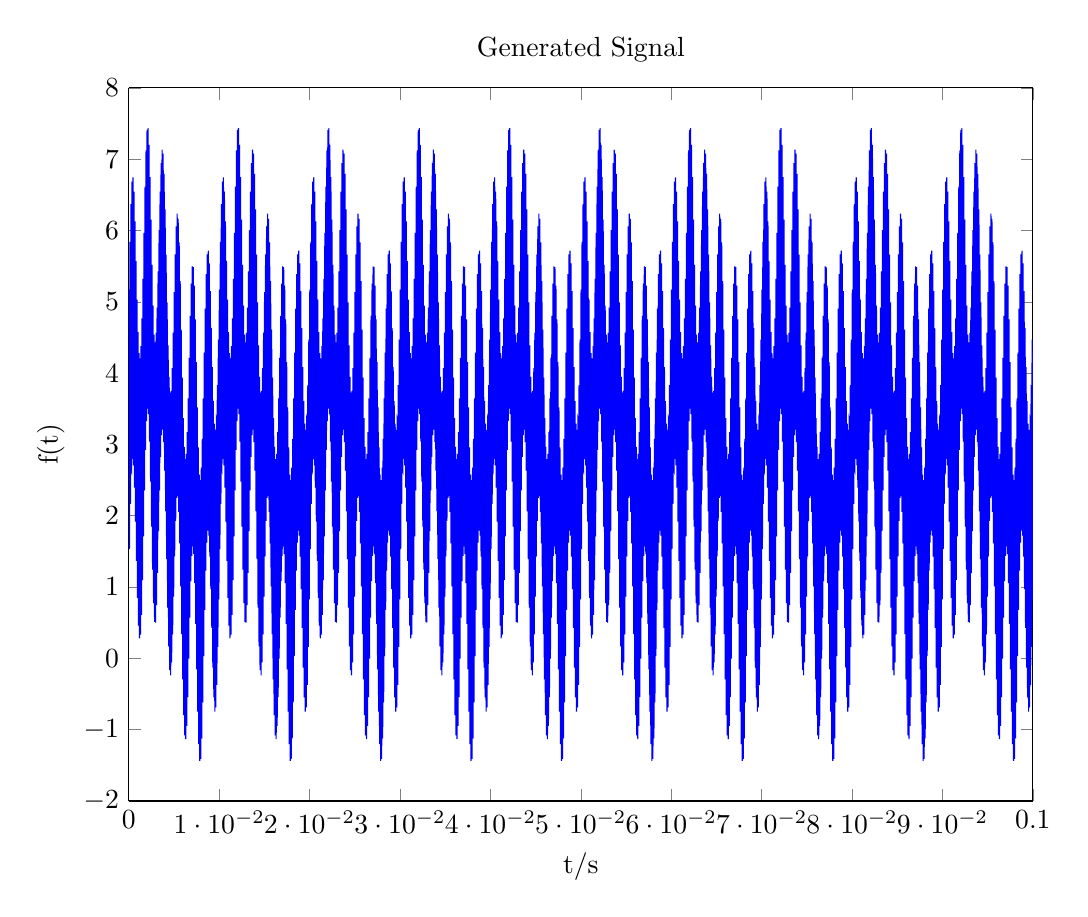
\begin{tikzpicture}

\begin{axis}[%
width=4.520833in,
height=3.565625in,
at={(0.758333in,0.48125in)},
scale only axis,
separate axis lines,
every outer x axis line/.append style={black},
every x tick label/.append style={font=\color{black}},
xmin=0,
xmax=0.1,
xlabel={t/s},
every outer y axis line/.append style={black},
every y tick label/.append style={font=\color{black}},
ymin=-2,
ymax=8,
ylabel={f(t)},
title={Generated Signal}
]
\addplot [color=blue,solid,forget plot]
  table[row sep=crcr]{%
0	3\\
1e-05	4.13447200792845\\
2e-05	4.93521035310729\\
3e-05	5.17236241965459\\
4e-05	4.79149496467605\\
5e-05	3.93051671970661\\
6e-05	2.8767165497643\\
7e-05	1.97729312290989\\
8e-05	1.53123218908794\\
9e-05	1.69619487949\\
0.0001	2.43940684397138\\
0.00011	3.54783864022627\\
0.00012	4.69450780370776\\
0.00013	5.54025986990388\\
0.00014	5.83933945586093\\
0.00015	5.5158824945369\\
0.00016	4.68751424391071\\
0.00017	3.62870599969009\\
0.00018	2.68529921495215\\
0.00019	2.16680947146704\\
0.0002	2.25004085986703\\
0.00021	2.92401989540883\\
0.00022	3.99339349959329\\
0.00023	5.13923313219957\\
0.00024	6.01831408832972\\
0.00025	6.36995995660265\\
0.00026	6.09718686499263\\
0.00027	5.29688375053492\\
0.00028	4.22963222385095\\
0.00029	3.23856245735008\\
0.0003	2.64250886069445\\
0.00031	2.6367309168424\\
0.00032	3.23210918234195\\
0.00033	4.25174743709056\\
0.00034	5.38603889881748\\
0.00035	6.28905197183938\\
0.00036	6.68622640315821\\
0.00037	6.45984928855812\\
0.00038	5.68569848377213\\
0.00039	4.60944471720873\\
0.0004	3.57015947522232\\
0.00041	2.89474403783183\\
0.00042	2.79614857113824\\
0.00043	3.30707016938658\\
0.00044	4.26977257490238\\
0.00045	5.38519714676085\\
0.00046	6.30607466433336\\
0.00047	6.7450481480336\\
0.00048	6.56414328588108\\
0.00049	5.81773036696989\\
0.0005	4.73560176881768\\
0.00051	3.65143371617812\\
0.00052	2.89890531512685\\
0.00053	2.70781758305348\\
0.00054	3.1325551951983\\
0.00055	4.03516395156119\\
0.00056	5.12831268179471\\
0.00057	6.0647636350973\\
0.00058	6.5454952562464\\
0.00059	6.4128139364528\\
0.0006	5.69946492143331\\
0.00061	4.61845196293269\\
0.00062	3.49673528465023\\
0.00063	2.67345059090888\\
0.00064	2.39433801113204\\
0.00065	2.73524988650792\\
0.00066	3.57855277688623\\
0.00067	4.6497707590412\\
0.00068	5.60306131295207\\
0.00069	6.12891135134133\\
0.0007	6.05052283530795\\
0.00071	5.37887884931338\\
0.00072	4.30934560526946\\
0.00073	3.16086829119145\\
0.00074	2.27669174984777\\
0.00075	1.91751599130197\\
0.00076	2.18035191289345\\
0.00077	2.96834099048291\\
0.00078	4.02093537006556\\
0.00079	4.99504193095764\\
0.0008	5.57186655703848\\
0.00081	5.55619324280871\\
0.00082	4.93718803067531\\
0.00083	3.89179679433597\\
0.00084	2.7296789531014\\
0.00085	1.79682164770651\\
0.00086	1.36784350464814\\
0.00087	1.56051854650603\\
0.00088	2.29913269329495\\
0.00089	3.33808155848227\\
0.0009	4.33836246881667\\
0.00091	4.97314533019842\\
0.00092	5.02955343348083\\
0.00093	4.47496530740137\\
0.00094	3.46719489056209\\
0.00095	2.30538045175462\\
0.00096	1.33687267264294\\
0.00097	0.849111710643196\\
0.00098	0.980156653548294\\
0.00099	1.6757234649783\\
0.001	2.70610737385376\\
0.00101	3.73772099048355\\
0.00102	4.4369751456354\\
0.00103	4.57415973213644\\
0.00104	4.0949818285479\\
0.00105	3.13748810127074\\
0.00106	1.98910276765646\\
0.00107	0.997157073294764\\
0.00108	0.460766382527009\\
0.00109	0.537718293693981\\
0.0011	1.19536159691072\\
0.00111	2.22078648832871\\
0.00112	3.28712647012046\\
0.00113	4.05533920803906\\
0.00114	4.27977745367812\\
0.00115	3.88468112524116\\
0.00116	2.98777516896432\\
0.00117	1.86362613024529\\
0.00118	0.858166138013741\\
0.00119	0.280996747285292\\
0.0012	0.309003197245347\\
0.00121	0.931288211783095\\
0.00122	1.95256987290421\\
0.00123	3.05398565173272\\
0.00124	3.89237161184199\\
0.00125	4.20710678118655\\
0.00126	3.90125731925243\\
0.00127	3.07175671576106\\
0.00128	1.97922559197929\\
0.00129	0.966827533582796\\
0.0013	0.353424718738071\\
0.00131	0.334298714785433\\
0.00132	0.920346447250909\\
0.00133	1.93468232644733\\
0.00134	3.06770444695425\\
0.00135	3.97348032954798\\
0.00136	4.37744307866127\\
0.00137	4.16186739802689\\
0.00138	3.40251301956244\\
0.00139	2.34502684196146\\
0.0014	1.32845084993781\\
0.00141	0.679651191979597\\
0.00142	0.611537322803333\\
0.00143	1.15676010338324\\
0.00144	2.15753158670276\\
0.00145	3.31473605999348\\
0.00146	4.28104192950115\\
0.00147	4.76902462998599\\
0.00148	4.64063714744874\\
0.00149	3.9501720560336\\
0.0015	2.92733911593625\\
0.00151	1.90572714974283\\
0.00152	1.2189232008432\\
0.00153	1.09663169437406\\
0.00154	1.59313632114463\\
0.00155	2.57037764817708\\
0.00156	3.74091517326974\\
0.00157	4.75739787038613\\
0.00158	5.3206871267887\\
0.00159	5.27296866036971\\
0.0016	4.64686359933969\\
0.00161	3.65524831026064\\
0.00162	2.62495254512833\\
0.00163	1.8949786355846\\
0.00164	1.71093062706029\\
0.00165	2.14852225896009\\
0.00166	3.08997916865847\\
0.00167	4.26068239016097\\
0.00168	5.31464444379656\\
0.00169	5.9422055718933\\
0.0017	5.96641956298063\\
0.00171	5.39812003748026\\
0.00172	4.43252266433514\\
0.00173	3.38842122373787\\
0.00174	2.6089085010855\\
0.00175	2.35453201575079\\
0.00176	2.72214995790901\\
0.00177	3.6147510969378\\
0.00178	4.77163509018488\\
0.00179	5.84955676300066\\
0.0018	6.52957059620891\\
0.00181	6.61631004747063\\
0.00182	6.09879170264375\\
0.00183	5.15381327170835\\
0.00184	4.09088751379346\\
0.00185	3.25585662155712\\
0.00186	2.92319619166071\\
0.00187	3.2105393385016\\
0.00188	4.0420333959629\\
0.00189	5.17193791052957\\
0.0019	6.26111685463689\\
0.00191	6.98260968220647\\
0.00192	7.12341231998976\\
0.00193	6.65077920165422\\
0.00194	5.72240361627405\\
0.00195	4.63730680027014\\
0.00196	3.74272618656815\\
0.00197	3.32599262857834\\
0.00198	3.52506001031439\\
0.00199	4.2855433415131\\
0.002	5.37764129073788\\
0.00201	6.46767443885433\\
0.00202	7.22196624905069\\
0.00203	7.41072403276416\\
0.00204	6.97957719088074\\
0.00205	6.06649972639853\\
0.00206	4.95884831097111\\
0.00207	4.0038918583562\\
0.00208	3.50068870368162\\
0.00209	3.60697479991089\\
0.0021	4.29005274918611\\
0.00211	5.33697208290346\\
0.00212	6.42083121966311\\
0.00213	7.20255837286366\\
0.00214	7.43648251499541\\
0.00215	7.04682549238159\\
0.00216	6.15129991246361\\
0.00217	5.02446573264614\\
0.00218	4.01225425421178\\
0.00219	3.42427196623488\\
0.0022	3.43741479683741\\
0.00221	4.04080189871827\\
0.00222	5.03917349940489\\
0.00223	6.11369490097119\\
0.00224	6.92123564400564\\
0.00225	7.20121383215756\\
0.00226	6.85674024394685\\
0.00227	5.98479846824993\\
0.00228	4.84606463460527\\
0.00229	3.78376316738602\\
0.0023	3.11682232761719\\
0.00231	3.04059491594198\\
0.00232	3.56605414059867\\
0.00233	4.51639563581181\\
0.00234	5.58210354604083\\
0.00235	6.41733614582149\\
0.00236	6.74762186845336\\
0.00237	6.45533518636976\\
0.00238	5.61633989844045\\
0.00239	4.4763911208731\\
0.0024	3.37464305287035\\
0.00241	2.63807789511695\\
0.00242	2.47972482751419\\
0.00243	2.93235793927014\\
0.00244	3.838315839735\\
0.00245	4.89861252099426\\
0.00246	5.76604905851605\\
0.00247	6.15333633231999\\
0.00248	5.92256535742776\\
0.00249	5.12816912481904\\
0.0025	4\\
0.00251	2.87179139689325\\
0.00252	2.07727673097988\\
0.00253	1.84630837244163\\
0.00254	2.23331932005059\\
0.00255	3.10040059973725\\
0.00256	4.16026310554623\\
0.00257	5.0657079300861\\
0.00258	5.51774908569784\\
0.00259	5.35872520510099\\
0.0026	4.6214104039862\\
0.00261	3.51883389184935\\
0.00262	2.37797790208078\\
0.00263	1.53799666969827\\
0.00264	1.24464534983299\\
0.00265	1.57378778338469\\
0.00266	2.40779848792182\\
0.00267	3.47220594498218\\
0.00268	4.42116848044134\\
0.00269	4.94517029319764\\
0.0027	4.86740707501175\\
0.00271	4.19885209475295\\
0.00272	3.13485821678799\\
0.00273	1.99435376895532\\
0.00274	1.12056324552895\\
0.00275	0.774162849032717\\
0.00276	1.05213624441013\\
0.00277	1.85759428932683\\
0.00278	2.92995516965354\\
0.00279	3.9260885112724\\
0.0028	4.52715970461997\\
0.00281	4.53790906865179\\
0.00282	3.94745585055674\\
0.00283	2.93269607600484\\
0.00284	1.80323633467276\\
0.00285	0.905008031495895\\
0.00286	0.512571230577743\\
0.00287	0.743638649100601\\
0.00288	1.52243224616628\\
0.00289	2.6032811100768\\
0.0029	3.64711357307119\\
0.00291	4.327028175614\\
0.00292	4.43007457398492\\
0.00293	3.92355549822379\\
0.00294	2.96520703220101\\
0.00295	1.85408764495531\\
0.00296	0.937466387153979\\
0.00297	0.502700070353502\\
0.00298	0.687762840442605\\
0.00299	1.43828424418007\\
0.003	2.5244717418524\\
0.00301	3.61264894846745\\
0.00302	4.36913659967509\\
0.00303	4.56413352178127\\
0.00304	4.14325488521753\\
0.00305	3.24445473763829\\
0.00306	2.15506409903365\\
0.00307	1.22232057184213\\
0.00308	0.745245564923453\\
0.00309	0.881532542709968\\
0.0031	1.59843611713965\\
0.00311	2.6829523961398\\
0.00312	3.80812101770606\\
0.00313	4.63480614123865\\
0.00314	4.91726750307104\\
0.00315	4.57965262981082\\
0.00316	3.73959483144838\\
0.00317	2.67156990309867\\
0.00318	1.72142023872623\\
0.00319	1.1986588016116\\
0.0032	1.28008350872314\\
0.00321	1.95471115573576\\
0.00322	3.02717541294783\\
0.00323	4.17853097663272\\
0.00324	5.06553289039354\\
0.00325	5.42748103262595\\
0.00326	5.16736439654156\\
0.00327	4.38204139892697\\
0.00328	3.33205978853469\\
0.00329	2.36051258290082\\
0.0033	1.78619379710709\\
0.00331	1.80431933772654\\
0.00332	2.42572306554249\\
0.00333	3.47345901216801\\
0.00334	4.63786766572719\\
0.00335	5.57296179504781\\
0.00336	6.00412268532702\\
0.00337	5.81357622781398\\
0.00338	5.07703641846104\\
0.00339	4.04010756190954\\
0.0034	3.04179225166435\\
0.00341	2.40892050422663\\
0.00342	2.35436895329558\\
0.00343	2.91075899684027\\
0.00344	3.92027662512196\\
0.00345	5.08378350037212\\
0.00346	6.05392887411228\\
0.00347	6.54327252427685\\
0.00348	6.41375530059117\\
0.00349	5.71966117912337\\
0.0035	4.69069487281365\\
0.00351	3.66044371538862\\
0.00352	2.962496822293\\
0.00353	2.82656424909115\\
0.00354	3.30693886779454\\
0.00355	4.26557396475792\\
0.00356	5.41504527757044\\
0.00357	6.40802151776995\\
0.00358	6.94538728033073\\
0.00359	6.86935492841787\\
0.0036	6.2125756356137\\
0.00361	5.18795917165722\\
0.00362	4.12237200246039\\
0.00363	3.35485643255055\\
0.00364	3.13105968281094\\
0.00365	3.52674180971295\\
0.00366	4.42417784389414\\
0.00367	5.54880121903017\\
0.00368	6.55467978746547\\
0.00369	7.13221197765969\\
0.0037	7.10451253610475\\
0.00371	6.48247872679133\\
0.00372	5.46139245779651\\
0.00373	4.36011625028264\\
0.00374	3.52181403516613\\
0.00375	3.20710678118655\\
0.00376	3.51292832775572\\
0.00377	4.34234518625422\\
0.00378	5.43473673872145\\
0.00379	6.44693940499166\\
0.0038	7.06009101461204\\
0.00381	7.07891001015953\\
0.00382	6.49249947822829\\
0.00383	5.47774502282805\\
0.00384	4.34424856590416\\
0.00385	3.43794260540615\\
0.00386	3.03339405782779\\
0.00387	3.2483282425627\\
0.00388	4.00698545301847\\
0.00389	5.0637188180245\\
0.0039	6.07948638258664\\
0.00391	6.72742203013228\\
0.00392	6.79461634005437\\
0.00393	6.24841848768145\\
0.00394	5.24661645852422\\
0.00395	4.08832600603516\\
0.00396	3.12087876684132\\
0.00397	2.6316993512416\\
0.00398	2.75883482047964\\
0.00399	3.4479926498386\\
0.004	4.46946313073117\\
0.00401	5.48965749435888\\
0.00402	6.17498875329625\\
0.00403	6.29575254054598\\
0.00404	5.79766522561058\\
0.00405	4.81878630394959\\
0.00406	3.6465563424143\\
0.00407	2.62832643385541\\
0.00408	2.0632352599877\\
0.00409	2.10909717405537\\
0.0041	2.73329112114137\\
0.00411	3.72294081013118\\
0.00412	4.75121656662768\\
0.00413	5.47911613873539\\
0.00414	5.66103556291487\\
0.00415	5.22126118379424\\
0.00416	4.27756745017007\\
0.00417	3.10457341634302\\
0.00418	2.04826665242122\\
0.00419	1.41830700864195\\
0.0042	1.39164079116496\\
0.00421	1.95743447637823\\
0.00422	2.92047249426516\\
0.00423	3.96196116567201\\
0.00424	4.73880780834956\\
0.00425	4.99046500817712\\
0.00426	4.62007468233228\\
0.00427	3.72464817088634\\
0.00428	2.56488592803245\\
0.00429	1.48403324204848\\
0.0043	0.801035747822192\\
0.00431	0.711260105482297\\
0.00432	1.22568984903451\\
0.00433	2.16752739043156\\
0.00434	3.22726009454111\\
0.00435	4.05904589476167\\
0.00436	4.38840932254237\\
0.00437	4.09771739364588\\
0.00438	3.26282290639337\\
0.00439	2.12946644854283\\
0.0044	1.03678418393604\\
0.00441	0.311736796956263\\
0.00442	0.167328501180099\\
0.00443	0.636305005285229\\
0.00444	1.56097316455434\\
0.00445	2.64231188892935\\
0.00446	3.53308389384768\\
0.00447	3.9459584762564\\
0.00448	3.74298190448753\\
0.00449	2.97853932313248\\
0.0045	1.88243221993214\\
0.00451	0.788340172295638\\
0.00452	0.0299398772729527\\
0.00453	-0.162975814377045\\
0.00454	0.263963860606643\\
0.00455	1.17278506531758\\
0.00456	2.27613129613235\\
0.00457	3.22673380925415\\
0.00458	3.72553444144156\\
0.00459	3.61479741353495\\
0.0046	2.92722029910733\\
0.00461	1.87575374438212\\
0.00462	0.787299510275346\\
0.00463	0.000929564795071336\\
0.00464	-0.237684881259455\\
0.00465	0.147234510953684\\
0.00466	1.03797532102661\\
0.00467	2.1599777804493\\
0.00468	3.16731077868693\\
0.00469	3.75036801925934\\
0.0047	3.73225376847698\\
0.00471	3.12384906990414\\
0.00472	2.12041389409962\\
0.00473	1.04078313889047\\
0.00474	0.228087465397148\\
0.00475	-0.0570910265221896\\
0.00476	0.282137089911788\\
0.00477	1.14878843290502\\
0.00478	2.28218708177596\\
0.00479	3.33910882277572\\
0.0048	4.00062560726157\\
0.00481	4.0713848487227\\
0.00482	3.54041355479483\\
0.00483	2.58451630886045\\
0.00484	1.51320918579174\\
0.00485	0.672334132100134\\
0.00486	0.33636293724056\\
0.00487	0.622921353232425\\
0.00488	1.45614580734819\\
0.00489	2.59028141120264\\
0.0049	3.68617419508732\\
0.00491	4.41684218947404\\
0.00492	4.56925644727158\\
0.00493	4.11064311372585\\
0.00494	3.19866381557548\\
0.00495	2.13230479844966\\
0.00496	1.25876522621063\\
0.00497	0.86533445977623\\
0.00498	1.08992172665941\\
0.00499	1.87809428000266\\
0.005	2.99999999999999\\
0.00501	4.12190571999733\\
0.00502	4.91007827334058\\
0.00503	5.13466554022377\\
0.00504	4.74123477378938\\
0.00505	3.86769520155036\\
0.00506	2.80133618442443\\
0.00507	1.88935688627408\\
0.00508	1.4307435527284\\
0.00509	1.58315781052599\\
0.0051	2.31382580491276\\
0.00511	3.40971858879758\\
0.00512	4.5438541926519\\
0.00513	5.37707864676756\\
0.00514	5.66363706275944\\
0.00515	5.32766586789987\\
0.00516	4.48679081420827\\
0.00517	3.41548369113956\\
0.00518	2.45958644520519\\
0.00519	1.9286151512773\\
0.0052	1.99937439273843\\
0.00521	2.66089117722427\\
0.00522	3.71781291822403\\
0.00523	4.85121156709507\\
0.00524	5.71786291008821\\
0.00525	6.05709102652219\\
0.00526	5.7719125346028\\
0.00527	4.95921686110944\\
0.00528	3.87958610590028\\
0.00529	2.87615093009579\\
0.0053	2.26774623152299\\
0.00531	2.24963198074069\\
0.00532	2.83268922131314\\
0.00533	3.8400222195508\\
0.00534	4.96202467897338\\
0.00535	5.85276548904631\\
0.00536	6.23768488125945\\
0.00537	5.99907043520494\\
0.00538	5.21270048972467\\
0.00539	4.1242462556179\\
0.0054	3.07277970089259\\
0.00541	2.38520258646506\\
0.00542	2.27446555855845\\
0.00543	2.77326619074584\\
0.00544	3.72386870386774\\
0.00545	4.8272149346824\\
0.00546	5.73603613939342\\
0.00547	6.16297581437704\\
0.00548	5.970060122727\\
0.00549	5.21165982770433\\
0.0055	4.11756778006776\\
0.00551	3.02146067686749\\
0.00552	2.25701809551243\\
0.00553	2.0540415237436\\
0.00554	2.46691610615235\\
0.00555	3.35768811107064\\
0.00556	4.4390268354457\\
0.00557	5.3636949947148\\
0.00558	5.83267149881991\\
0.00559	5.6882632030437\\
0.0056	4.96321581606392\\
0.00561	3.87053355145707\\
0.00562	2.7371770936066\\
0.00563	1.90228260635407\\
0.00564	1.61159067745763\\
0.00565	1.94095410523838\\
0.00566	2.77273990545882\\
0.00567	3.83247260956854\\
0.00568	4.77431015096552\\
0.00569	5.28873989451772\\
0.0057	5.1989642521778\\
0.00571	4.51596675795143\\
0.00572	3.43511407196757\\
0.00573	2.27535182911361\\
0.00574	1.37992531766769\\
0.00575	1.00953499182287\\
0.00576	1.26119219165049\\
0.00577	2.03803883432802\\
0.00578	3.07952750573493\\
0.00579	4.0425655236218\\
0.0058	4.60835920883506\\
0.00581	4.58169299135806\\
0.00582	3.9517333475787\\
0.00583	2.89542658365705\\
0.00584	1.72243254982983\\
0.00585	0.778738816205799\\
0.00586	0.338964437085119\\
0.00587	0.520883861264629\\
0.00588	1.2487834333724\\
0.00589	2.27705918986886\\
0.0059	3.26670887885871\\
0.00591	3.89090282594468\\
0.00592	3.93676474001228\\
0.00593	3.37167356614448\\
0.00594	2.35344365758566\\
0.00595	1.18121369605031\\
0.00596	0.202334774389395\\
0.00597	-0.295752540545995\\
0.00598	-0.174988753296274\\
0.00599	0.510342505641196\\
0.006	1.53053686926876\\
0.00601	2.55200735016148\\
0.00602	3.24116517952033\\
0.00603	3.36830064875838\\
0.00604	2.87912123315873\\
0.00605	1.91167399396474\\
0.00606	0.75338354147585\\
0.00607	-0.248418487681515\\
0.00608	-0.794616340054406\\
0.00609	-0.727422030132247\\
0.0061	-0.0794863825866061\\
0.00611	0.9362811819756\\
0.00612	1.99301454698162\\
0.00613	2.75167175743732\\
0.00614	2.9666059421722\\
0.00615	2.56205739459389\\
0.00616	1.65575143409574\\
0.00617	0.52225497717191\\
0.00618	-0.492499478228364\\
0.00619	-1.07891001015954\\
0.0062	-1.06009101461201\\
0.00621	-0.44693940499163\\
0.00622	0.565263261278646\\
0.00623	1.65765481374572\\
0.00624	2.48707167224434\\
0.00625	2.79289321881345\\
0.00626	2.47818596483382\\
0.00627	1.63988374971732\\
0.00628	0.538607542203395\\
0.00629	-0.482478726791357\\
0.0063	-1.10451253610478\\
0.00631	-1.13221197765967\\
0.00632	-0.554679787465485\\
0.00633	0.451198780969928\\
0.00634	1.57582215610585\\
0.00635	2.47325819028711\\
0.00636	2.86894031718906\\
0.00637	2.64514356744941\\
0.00638	1.87762799753958\\
0.00639	0.812040828342688\\
0.0064	-0.212575635613734\\
0.00641	-0.869354928417907\\
0.00642	-0.945387280330721\\
0.00643	-0.408021517769964\\
0.00644	0.584954722429494\\
0.00645	1.73442603524218\\
0.00646	2.69306113220553\\
0.00647	3.17343575090886\\
0.00648	3.03750317770696\\
0.00649	2.33955628461139\\
0.0065	1.30930512718625\\
0.00651	0.280338820876649\\
0.00652	-0.413755300591204\\
0.00653	-0.543272524276849\\
0.00654	-0.0539288741121768\\
0.00655	0.916216499627919\\
0.00656	2.07972337487819\\
0.00657	3.08924100315977\\
0.00658	3.64563104670444\\
0.00659	3.59107949577337\\
0.0066	2.95820774833557\\
0.00661	1.95989243809048\\
0.00662	0.922963581538979\\
0.00663	0.186423772186028\\
0.00664	-0.00412268532701621\\
0.00665	0.427038204952184\\
0.00666	1.36213233427279\\
0.00667	2.52654098783209\\
0.00668	3.5742769344575\\
0.00669	4.19568066227348\\
0.0067	4.21380620289291\\
0.00671	3.63948741709907\\
0.00672	2.66794021146527\\
0.00673	1.61795860107289\\
0.00674	0.832635603458421\\
0.00675	0.57251896737406\\
0.00676	0.934467109606477\\
0.00677	1.82146902336742\\
0.00678	2.97282458705216\\
0.00679	4.04528884426423\\
0.0068	4.71991649127686\\
0.00681	4.80134119838841\\
0.00682	4.27857976127379\\
0.00683	3.32843009690135\\
0.00684	2.26040516855163\\
0.00685	1.42034737018916\\
0.00686	1.08273249692896\\
0.00687	1.36519385876136\\
0.00688	2.19187898229407\\
0.00689	3.31704760386024\\
0.0069	4.40156388286048\\
0.00691	5.11846745729005\\
0.00692	5.25475443507652\\
0.00693	4.77767942815784\\
0.00694	3.8449359009662\\
0.00695	2.75554526236167\\
0.00696	1.85674511478245\\
0.00697	1.43586647821873\\
0.00698	1.63086340032491\\
0.00699	2.38735105153253\\
0.007	3.47552825814759\\
0.00701	4.56171575581991\\
0.00702	5.31223715955741\\
0.00703	5.49729992964649\\
0.00704	5.062533612846\\
0.00705	4.14591235504465\\
0.00706	3.03479296779895\\
0.00707	2.0764445017761\\
0.00708	1.56992542601507\\
0.00709	1.67297182438606\\
0.0071	2.35288642692884\\
0.00711	3.39671888992335\\
0.00712	4.47756775383365\\
0.00713	5.25636135089942\\
0.00714	5.48742876942225\\
0.00715	5.09499196850408\\
0.00716	4.1967636653271\\
0.00717	3.06730392399517\\
0.00718	2.05254414944327\\
0.00719	1.4620909313482\\
0.0072	1.47284029538008\\
0.00721	2.07391148872763\\
0.00722	3.0700448303465\\
0.00723	4.14240571067321\\
0.00724	4.94786375558996\\
0.00725	5.22583715096728\\
0.00726	4.87943675447102\\
0.00727	4.00564623104464\\
0.00728	2.86514178321186\\
0.00729	1.8011479052471\\
0.0073	1.13259292498823\\
0.00731	1.05482970680237\\
0.00732	1.57883151955869\\
0.00733	2.52779405501775\\
0.00734	3.59220151207823\\
0.00735	4.42621221661533\\
0.00736	4.75535465016701\\
0.00737	4.46200333030162\\
0.00738	3.62202209791919\\
0.00739	2.4811661081506\\
0.0074	1.37858959601377\\
0.00741	0.641274794898942\\
0.00742	0.482250914302144\\
0.00743	0.934292069913924\\
0.00744	1.83973689445381\\
0.00745	2.89959940026289\\
0.00746	3.76668067994937\\
0.00747	4.15369162755838\\
0.00748	3.9227232690201\\
0.00749	3.12820860310662\\
0.0075	2.00000000000007\\
0.00751	0.871830875180929\\
0.00752	0.0774346425722241\\
0.00753	-0.153336332319994\\
0.00754	0.233950941483944\\
0.00755	1.10138747900583\\
0.00756	2.16168416026509\\
0.00757	3.06764206072989\\
0.00758	3.52027517248584\\
0.00759	3.36192210488303\\
0.0076	2.62535694712962\\
0.00761	1.52360887912686\\
0.00762	0.383660101559402\\
0.00763	-0.455335186369727\\
0.00764	-0.747621868453356\\
0.00765	-0.417336145821441\\
0.00766	0.417896453959362\\
0.00767	1.48360436418811\\
0.00768	2.43394585940136\\
0.00769	2.95940508405802\\
0.0077	2.88317767238282\\
0.00771	2.21623683261399\\
0.00772	1.15393536539463\\
0.00773	0.0152015317499723\\
0.00774	-0.856740243946843\\
0.00775	-1.20121383215756\\
0.00776	-0.921235644005585\\
0.00777	-0.113694900971127\\
0.00778	0.960826500595177\\
0.00779	1.95919810128187\\
0.0078	2.56258520316257\\
0.00781	2.5757280337651\\
0.00782	1.98774574578816\\
0.00783	0.975534267353907\\
0.00784	-0.151299912463783\\
0.00785	-1.04682549238163\\
0.00786	-1.43648251499542\\
0.00787	-1.20255837286368\\
0.00788	-0.420831219663119\\
0.00789	0.663027917096641\\
0.0079	1.70994725081397\\
0.00791	2.3930252000891\\
0.00792	2.49931129631839\\
0.00793	1.99610814164374\\
0.00794	1.04115168902879\\
0.00795	-0.0664997263985172\\
0.00796	-0.979577190880732\\
0.00797	-1.41072403276418\\
0.00798	-1.22196624905066\\
0.00799	-0.467674438854274\\
0.008	0.62235870926208\\
0.00801	1.71445665848705\\
0.00802	2.47493998968564\\
0.00803	2.67400737142165\\
0.00804	2.25727381343184\\
0.00805	1.3626931997299\\
0.00806	0.277596383725858\\
0.00807	-0.650779201654282\\
0.00808	-1.12341231998976\\
0.00809	-0.982609682206478\\
0.0081	-0.261116854636805\\
0.00811	0.828062089470526\\
0.00812	1.95796660403709\\
0.00813	2.78946066149839\\
0.00814	3.07680380833929\\
0.00815	2.74414337844283\\
0.00816	1.90911248620645\\
0.00817	0.846186728291668\\
0.00818	-0.0987917026439171\\
0.00819	-0.616310047470656\\
0.0082	-0.529570596208865\\
0.00821	0.150443236999352\\
0.00822	1.22836490981507\\
0.00823	2.3852489030623\\
0.00824	3.27785004209105\\
0.00825	3.64546798424921\\
0.00826	3.39109149891451\\
0.00827	2.61157877626202\\
0.00828	1.56747733566474\\
0.00829	0.601879962519749\\
0.0083	0.0335804370193822\\
0.00831	0.057794428106706\\
0.00832	0.685355556203524\\
0.00833	1.73931760983902\\
0.00834	2.91002083134152\\
0.00835	3.85147774104005\\
0.00836	4.28906937293972\\
0.00837	4.10502136441534\\
0.00838	3.37504745487166\\
0.00839	2.34475168973938\\
0.0084	1.35313640066024\\
0.00841	0.727031339630257\\
0.00842	0.679312873211299\\
0.00843	1.24260212961387\\
0.00844	2.25908482673039\\
0.00845	3.42962235182304\\
0.00846	4.40686367885538\\
0.00847	4.90336830562594\\
0.00848	4.78107679915676\\
0.00849	4.09427285025708\\
0.0085	3.07266088406377\\
0.00851	2.04982794396639\\
0.00852	1.35936285255126\\
0.00853	1.23097537001403\\
0.00854	1.71895807049886\\
0.00855	2.68526394000653\\
0.00856	3.84246841329714\\
0.00857	4.84323989661685\\
0.00858	5.3884626771967\\
0.00859	5.3203488080204\\
0.0086	4.67154915006218\\
0.00861	3.65497315803841\\
0.00862	2.59748698043745\\
0.00863	1.8381326019731\\
0.00864	1.62255692133873\\
0.00865	2.0265196704521\\
0.00866	2.93229555304587\\
0.00867	4.06531767355268\\
0.00868	5.07965355274912\\
0.00869	5.66570128521457\\
0.0087	5.64657528126189\\
0.00871	5.0331724664172\\
0.00872	4.0207744080207\\
0.00873	2.92824328423904\\
0.00874	2.0987426807475\\
0.00875	1.79289321881345\\
0.00876	2.10762838815801\\
0.00877	2.94601434826732\\
0.00878	4.04743012709595\\
0.00879	5.068711788217\\
0.0088	5.69099680275466\\
0.00881	5.7190032527147\\
0.00882	5.14183386198616\\
0.00883	4.13637386975456\\
0.00884	3.01222483103567\\
0.00885	2.11531887475882\\
0.00886	1.72022254632187\\
0.00887	1.94466079196101\\
0.00888	2.71287352987958\\
0.00889	3.77921351167132\\
0.0089	4.80463840308921\\
0.00891	5.46228170630607\\
0.00892	5.53923361747298\\
0.00893	5.00284292670523\\
0.00894	4.01089723234362\\
0.00895	2.86251189872911\\
0.00896	1.905018171452\\
0.00897	1.42584026786355\\
0.00898	1.56302485436463\\
0.00899	2.26227900951656\\
0.009	3.29389262614638\\
0.00901	4.32427653502172\\
0.00902	5.01984334645173\\
0.00903	5.15088828935679\\
0.00904	4.66312732735696\\
0.00905	3.69461954824534\\
0.00906	2.53280510943776\\
0.00907	1.52503469259868\\
0.00908	0.970446566519139\\
0.00909	1.02685466980155\\
0.0091	1.66163753118328\\
0.00911	2.66191844151764\\
0.00912	3.70086730670518\\
0.00913	4.43948145349393\\
0.00914	4.63215649535186\\
0.00915	4.20317835229354\\
0.00916	3.27032104689845\\
0.00917	2.10820320566388\\
0.00918	1.06281196932473\\
0.00919	0.443806757191257\\
0.0092	0.428133442961558\\
0.00921	1.00495806904247\\
0.00922	1.97906462993439\\
0.00923	3.03165900951724\\
0.00924	3.81964808710652\\
0.00925	4.08248400869803\\
0.00926	3.72330825015226\\
0.00927	2.8391317088086\\
0.00928	1.6906543947306\\
0.00929	0.621121150686485\\
0.0093	-0.0505228353079419\\
0.00931	-0.12891135134134\\
0.00932	0.396938687047888\\
0.00933	1.35022924095896\\
0.00934	2.42144722311394\\
0.00935	3.26475011349204\\
0.00936	3.60566198886797\\
0.00937	3.32654940909104\\
0.00938	2.50326471534962\\
0.00939	1.38154803706736\\
0.0094	0.300535078566549\\
0.00941	-0.412813936452777\\
0.00942	-0.545495256246377\\
0.00943	-0.0647636350973348\\
0.00944	0.871687318205242\\
0.00945	1.96483604843876\\
0.00946	2.86744480480181\\
0.00947	3.29218241694651\\
0.00948	3.10109468487316\\
0.00949	2.34856628382192\\
0.0095	1.26439823118214\\
0.00951	0.182269633030145\\
0.00952	-0.564143285881066\\
0.00953	-0.745048148033602\\
0.00954	-0.306074664333242\\
0.00955	0.614802853239332\\
0.00956	1.73022742509758\\
0.00957	2.69292983061355\\
0.00958	3.20385142886175\\
0.00959	3.1052559621681\\
0.0096	2.42984052477772\\
0.00961	1.39055528279131\\
0.00962	0.314301516227904\\
0.00963	-0.459849288558215\\
0.00964	-0.686226403158215\\
0.00965	-0.289051971839409\\
0.00966	0.61396110118249\\
0.00967	1.74825256290964\\
0.00968	2.76789081765803\\
0.00969	3.36326908315759\\
0.0097	3.35749113930556\\
0.00971	2.76143754264979\\
0.00972	1.77036777614908\\
0.00973	0.703116249465112\\
0.00974	-0.0971868649926124\\
0.00975	-0.369959956602658\\
0.00976	-0.018314088329606\\
0.00977	0.860766867800399\\
0.00978	2.00660650040691\\
0.00979	3.07598010459114\\
0.0098	3.74995914013303\\
0.00981	3.83319052853297\\
0.00982	3.31470078504786\\
0.00983	2.37129400030993\\
0.00984	1.31248575608911\\
0.00985	0.484117505463118\\
0.00986	0.160660544139079\\
0.00987	0.459740130096105\\
0.00988	1.30549219629242\\
0.00989	2.45216135977371\\
0.0099	3.5605931560286\\
0.00991	4.30380512051\\
0.00992	4.46876781091205\\
0.00993	4.02270687708998\\
0.00994	3.12328345023572\\
0.00995	2.0694832802932\\
0.00996	1.20850503532396\\
0.00997	0.827637580345395\\
0.00998	1.06478964689271\\
0.00999	1.86552799207153\\
0.01	2.99999999999998\\
0.01001	4.13447200792864\\
0.01002	4.93521035310729\\
0.01003	5.1723624196546\\
0.01004	4.79149496467605\\
0.01005	3.93051671970642\\
0.01006	2.87671654976431\\
0.01007	1.9772931229099\\
0.01008	1.53123218908795\\
0.01009	1.69619487949\\
0.0101	2.43940684397138\\
0.01011	3.54783864022627\\
0.01012	4.69450780370775\\
0.01013	5.54025986990388\\
0.01014	5.83933945586092\\
0.01015	5.51588249453691\\
0.01016	4.68751424391071\\
0.01017	3.6287059996901\\
0.01018	2.68529921495199\\
0.01019	2.16680947146705\\
0.0102	2.25004085986703\\
0.01021	2.92401989540883\\
0.01022	3.99339349959352\\
0.01023	5.13923313219957\\
0.01024	6.01831408832972\\
0.01025	6.36995995660266\\
0.01026	6.09718686499263\\
0.01027	5.29688375053492\\
0.01028	4.22963222385095\\
0.01029	3.23856245735007\\
0.0103	2.64250886069444\\
0.01031	2.63673091684241\\
0.01032	3.23210918234195\\
0.01033	4.25174743709056\\
0.01034	5.38603889881748\\
0.01035	6.28905197183952\\
0.01036	6.68622640315822\\
0.01037	6.45984928855812\\
0.01038	5.68569848377212\\
0.01039	4.6094447172085\\
0.0104	3.57015947522231\\
0.01041	2.89474403783183\\
0.01042	2.79614857113825\\
0.01043	3.30707016938659\\
0.01044	4.26977257490239\\
0.01045	5.38519714676086\\
0.01046	6.30607466433337\\
0.01047	6.7450481480336\\
0.01048	6.56414328588107\\
0.01049	5.81773036696988\\
0.0105	4.73560176881766\\
0.01051	3.65143371617811\\
0.01052	2.89890531512675\\
0.01053	2.70781758305348\\
0.01054	3.13255519519832\\
0.01055	4.03516395156121\\
0.01056	5.12831268179494\\
0.01057	6.06476363509731\\
0.01058	6.5454952562464\\
0.01059	6.41281393645279\\
0.0106	5.69946492143329\\
0.01061	4.61845196293267\\
0.01062	3.49673528465021\\
0.01063	2.67345059090886\\
0.01064	2.39433801113204\\
0.01065	2.73524988650793\\
0.01066	3.57855277688624\\
0.01067	4.64977075904123\\
0.01068	5.60306131295208\\
0.01069	6.12891135134134\\
0.0107	6.05052283530794\\
0.01071	5.37887884931336\\
0.01072	4.30934560526944\\
0.01073	3.16086829119122\\
0.01074	2.27669174984776\\
0.01075	1.91751599130197\\
0.01076	2.18035191289347\\
0.01077	2.96834099048294\\
0.01078	4.02093537006558\\
0.01079	4.99504193095768\\
0.0108	5.57186655703849\\
0.01081	5.5561932428087\\
0.01082	4.93718803067529\\
0.01083	3.89179679433593\\
0.01084	2.72967895310136\\
0.01085	1.79682164770648\\
0.01086	1.36784350464813\\
0.01087	1.56051854650604\\
0.01088	2.29913269329499\\
0.01089	3.33808155848233\\
0.0109	4.33836246881669\\
0.01091	4.97314533019842\\
0.01092	5.02955343348082\\
0.01093	4.47496530740134\\
0.01094	3.46719489056227\\
0.01095	2.30538045175458\\
0.01096	1.33687267264292\\
0.01097	0.849111710643185\\
0.01098	0.980156653548312\\
0.01099	1.67572346497833\\
0.011	2.70610737385382\\
0.01101	3.73772099048359\\
0.01102	4.43697514563541\\
0.01103	4.57415973213643\\
0.01104	4.09498182854787\\
0.01105	3.1374881012707\\
0.01106	1.98910276765642\\
0.01107	0.997157073294714\\
0.01108	0.460766382526997\\
0.01109	0.537718293693996\\
0.0111	1.19536159691077\\
0.01111	2.22078648832853\\
0.01112	3.2871264701205\\
0.01113	4.05533920803908\\
0.01114	4.27977745367812\\
0.01115	3.88468112524113\\
0.01116	2.98777516896425\\
0.01117	1.86362613024525\\
0.01118	0.858166138013691\\
0.01119	0.280996747285274\\
0.0112	0.309003197245369\\
0.01121	0.931288211783148\\
0.01122	1.95256987290425\\
0.01123	3.05398565173276\\
0.01124	3.89237161184203\\
0.01125	4.20710678118655\\
0.01126	3.9012573192524\\
0.01127	3.07175671576099\\
0.01128	1.97922559197944\\
0.01129	0.966827533582743\\
0.0113	0.353424718738049\\
0.01131	0.334298714785451\\
0.01132	0.920346447250771\\
0.01133	1.9346823264474\\
0.01134	3.06770444695431\\
0.01135	3.97348032954802\\
0.01136	4.37744307866128\\
0.01137	4.16186739802686\\
0.01138	3.40251301956239\\
0.01139	2.34502684196139\\
0.0114	1.32845084993776\\
0.01141	0.679651191979564\\
0.01142	0.611537322803352\\
0.01143	1.15676010338329\\
0.01144	2.15753158670283\\
0.01145	3.31473605999333\\
0.01146	4.2810419295012\\
0.01147	4.769024629986\\
0.01148	4.64063714744872\\
0.01149	3.95017205603373\\
0.0115	2.92733911593616\\
0.01151	1.90572714974275\\
0.01152	1.21892320084317\\
0.01153	1.09663169437404\\
0.01154	1.59313632114468\\
0.01155	2.57037764817715\\
0.01156	3.74091517326981\\
0.01157	4.75739787038618\\
0.01158	5.32068712678873\\
0.01159	5.27296866036968\\
0.0116	4.64686359933962\\
0.01161	3.65524831026053\\
0.01162	2.62495254512847\\
0.01163	1.89497863558457\\
0.01164	1.7109306270603\\
0.01165	2.14852225896014\\
0.01166	3.08997916865835\\
0.01167	4.26068239016107\\
0.01168	5.31464444379663\\
0.01169	5.94220557189332\\
0.0117	5.96641956298067\\
0.01171	5.39812003748019\\
0.01172	4.43252266433509\\
0.01173	3.3884212237378\\
0.01174	2.60890850108545\\
0.01175	2.35453201575079\\
0.01176	2.72214995790907\\
0.01177	3.61475109693789\\
0.01178	4.77163509018501\\
0.01179	5.84955676300053\\
0.0118	6.52957059620894\\
0.01181	6.61631004747061\\
0.01182	6.09879170264371\\
0.01183	5.15381327170847\\
0.01184	4.09088751379338\\
0.01185	3.25585662155706\\
0.01186	2.9231961916607\\
0.01187	3.21053933850154\\
0.01188	4.04203339596299\\
0.01189	5.17193791052967\\
0.0119	6.26111685463697\\
0.01191	6.98260968220642\\
0.01192	7.12341231998975\\
0.01193	6.65077920165416\\
0.01194	5.72240361627396\\
0.01195	4.63730680027001\\
0.01196	3.74272618656825\\
0.01197	3.32599262857833\\
0.01198	3.52506001031444\\
0.01199	4.28554334151321\\
0.012	5.37764129073777\\
0.01201	6.46767443885444\\
0.01202	7.22196624905074\\
0.01203	7.41072403276414\\
0.01204	6.97957719088082\\
0.01205	6.06649972639844\\
0.01206	4.95884831097102\\
0.01207	4.00389185835613\\
0.01208	3.50068870368164\\
0.01209	3.60697479991093\\
0.0121	4.29005274918619\\
0.01211	5.33697208290355\\
0.01212	6.42083121966299\\
0.01213	7.20255837286361\\
0.01214	7.4364825149954\\
0.01215	7.04682549238151\\
0.01216	6.15129991246349\\
0.01217	5.02446573264624\\
0.01218	4.01225425421169\\
0.01219	3.42427196623484\\
0.0122	3.43741479683745\\
0.01221	4.04080189871819\\
0.01222	5.03917349940501\\
0.01223	6.1136949009713\\
0.01224	6.92123564400569\\
0.01225	7.20121383215756\\
0.01226	6.8567402439468\\
0.01227	5.98479846824984\\
0.01228	4.84606463460517\\
0.01229	3.78376316738612\\
0.0123	3.11682232761723\\
0.01231	3.04059491594202\\
0.01232	3.56605414059878\\
0.01233	4.51639563581197\\
0.01234	5.58210354604071\\
0.01235	6.41733614582155\\
0.01236	6.74762186845337\\
0.01237	6.45533518636968\\
0.01238	5.61633989844053\\
0.01239	4.47639112087294\\
0.0124	3.37464305287022\\
0.01241	2.6380778951169\\
0.01242	2.47972482751418\\
0.01243	2.93235793927024\\
0.01244	3.83831583973509\\
0.01245	4.89861252099436\\
0.01246	5.76604905851597\\
0.01247	6.15333633231997\\
0.01248	5.92256535742768\\
0.01249	5.1281691248189\\
0.0125	4.00000000000008\\
0.01251	2.87179139689331\\
0.01252	2.07727673097981\\
0.01253	1.84630837244165\\
0.01254	2.23331932005067\\
0.01255	3.10040059973718\\
0.01256	4.16026310554636\\
0.01257	5.06570793008621\\
0.01258	5.51774908569787\\
0.01259	5.35872520510102\\
0.0126	4.62141040398606\\
0.01261	3.51883389184919\\
0.01262	2.37797790208064\\
0.01263	1.53799666969834\\
0.01264	1.24464534983298\\
0.01265	1.57378778338478\\
0.01266	2.40779848792195\\
0.01267	3.47220594498211\\
0.01268	4.42116848044129\\
0.01269	4.94517029319763\\
0.0127	4.8674070750117\\
0.01271	4.198852094753\\
0.01272	3.13485821678806\\
0.01273	1.99435376895518\\
0.01274	1.12056324552886\\
0.01275	0.774162849032717\\
0.01276	1.05213624441008\\
0.01277	1.85759428932697\\
0.01278	2.92995516965369\\
0.01279	3.92608851127252\\
0.0128	4.52715970461995\\
0.01281	4.53790906865181\\
0.01282	3.94745585055658\\
0.01283	2.93269607600463\\
0.01284	1.80323633467282\\
0.01285	0.905008031495938\\
0.01286	0.512571230577746\\
0.01287	0.743638649100676\\
0.01288	1.52243224616622\\
0.01289	2.60328111007673\\
0.0129	3.64711357307131\\
0.01291	4.32702817561405\\
0.01292	4.43007457398489\\
0.01293	3.92355549822384\\
0.01294	2.96520703220086\\
0.01295	1.85408764495516\\
0.01296	0.93746638715388\\
0.01297	0.502700070353509\\
0.01298	0.687762840442575\\
0.01299	1.43828424418025\\
0.013	2.52447174185261\\
0.01301	3.61264894846744\\
0.01302	4.36913659967508\\
0.01303	4.56413352178128\\
0.01304	4.14325488521743\\
0.01305	3.24445473763836\\
0.01306	2.15506409903372\\
0.01307	1.22232057184219\\
0.01308	0.745245564923424\\
0.01309	0.881532542709946\\
0.0131	1.59843611713959\\
0.01311	2.68295239613996\\
0.01312	3.8081210177062\\
0.01313	4.63480614123873\\
0.01314	4.91726750307104\\
0.01315	4.57965262981086\\
0.01316	3.73959483144819\\
0.01317	2.67156990309847\\
0.01318	1.72142023872624\\
0.01319	1.19865880161161\\
0.0132	1.2800835087232\\
0.01321	1.95471115573594\\
0.01322	3.02717541294781\\
0.01323	4.17853097663266\\
0.01324	5.06553289039351\\
0.01325	5.42748103262595\\
0.01326	5.1673643965416\\
0.01327	4.38204139892703\\
0.01328	3.33205978853476\\
0.01329	2.36051258290071\\
0.0133	1.78619379710711\\
0.01331	1.80431933772654\\
0.01332	2.42572306554248\\
0.01333	3.47345901216822\\
0.01334	4.6378676657274\\
0.01335	5.57296179504779\\
0.01336	6.00412268532702\\
0.01337	5.81357622781387\\
0.01338	5.07703641846086\\
0.01339	4.04010756190955\\
0.0134	3.04179225166437\\
0.01341	2.40892050422665\\
0.01342	2.35436895329563\\
0.01343	2.91075899684021\\
0.01344	3.9202766251219\\
0.01345	5.08378350037205\\
0.01346	6.05392887411238\\
0.01347	6.54327252427685\\
0.01348	6.41375530059118\\
0.01349	5.71966117912337\\
0.0135	4.69069487281345\\
0.01351	3.66044371538844\\
0.01352	2.962496822293\\
0.01353	2.82656424909115\\
0.01354	3.30693886779467\\
0.01355	4.26557396475813\\
0.01356	5.41504527757048\\
0.01357	6.40802151776994\\
0.01358	6.94538728033072\\
0.01359	6.8693549284178\\
0.0136	6.21257563561376\\
0.01361	5.18795917165723\\
0.01362	4.12237200246045\\
0.01363	3.35485643255045\\
0.01364	3.13105968281094\\
0.01365	3.52674180971295\\
0.01366	4.42417784389412\\
0.01367	5.54880121903038\\
0.01368	6.55467978746546\\
0.01369	7.13221197765969\\
0.0137	7.10451253610475\\
0.01371	6.48247872679112\\
0.01372	5.4613924577963\\
0.01373	4.3601162502826\\
0.01374	3.52181403516613\\
0.01375	3.20710678118655\\
0.01376	3.51292832775583\\
0.01377	4.34234518625426\\
0.01378	5.43473673872143\\
0.01379	6.44693940499161\\
0.0138	7.0600910146121\\
0.01381	7.07891001015954\\
0.01382	6.49249947822831\\
0.01383	5.47774502282812\\
0.01384	4.34424856590397\\
0.01385	3.43794260540613\\
0.01386	3.03339405782779\\
0.01387	3.24832824256271\\
0.01388	4.00698545301865\\
0.01389	5.06371881802447\\
0.0139	6.07948638258667\\
0.01391	6.72742203013228\\
0.01392	6.79461634005439\\
0.01393	6.2484184876813\\
0.01394	5.24661645852418\\
0.01395	4.08832600603518\\
0.01396	3.12087876684128\\
0.01397	2.63169935124157\\
0.01398	2.75883482047966\\
0.01399	3.44799264983859\\
0.014	4.46946313073121\\
0.01401	5.48965749435906\\
0.01402	6.17498875329626\\
0.01403	6.29575254054597\\
0.01404	5.79766522561056\\
0.01405	4.81878630394938\\
0.01406	3.64655634241426\\
0.01407	2.62832643385547\\
0.01408	2.0632352599877\\
0.01409	2.10909717405542\\
0.0141	2.73329112114135\\
0.01411	3.72294081013121\\
0.01412	4.75121656662767\\
0.01413	5.47911613873539\\
0.01414	5.66103556291484\\
0.01415	5.22126118379422\\
0.01416	4.27756745017009\\
0.01417	3.10457341634298\\
0.01418	2.04826665242106\\
0.01419	1.41830700864194\\
0.0142	1.39164079116495\\
0.01421	1.95743447637827\\
0.01422	2.92047249426536\\
0.01423	3.96196116567226\\
0.01424	4.73880780834943\\
0.01425	4.99046500817712\\
0.01426	4.62007468233226\\
0.01427	3.7246481708863\\
0.01428	2.56488592803235\\
0.01429	1.48403324204851\\
0.0143	0.801035747822162\\
0.01431	0.711260105482357\\
0.01432	1.2256898490347\\
0.01433	2.16752739043131\\
0.01434	3.22726009454115\\
0.01435	4.05904589476166\\
0.01436	4.38840932254236\\
0.01437	4.0977173936459\\
0.01438	3.26282290639333\\
0.01439	2.12946644854262\\
0.0144	1.03678418393582\\
0.01441	0.311736796956354\\
0.01442	0.167328501180103\\
0.01443	0.636305005285256\\
0.01444	1.56097316455437\\
0.01445	2.64231188892944\\
0.01446	3.53308389384771\\
0.01447	3.94595847625641\\
0.01448	3.74298190448744\\
0.01449	2.97853932313263\\
0.0145	1.88243221993239\\
0.01451	0.788340172295607\\
0.01452	0.0299398772729553\\
0.01453	-0.162975814377045\\
0.01454	0.263963860606632\\
0.01455	1.17278506531767\\
0.01456	2.27613129613255\\
0.01457	3.22673380925437\\
0.01458	3.72553444144152\\
0.01459	3.61479741353491\\
0.0146	2.92722029910734\\
0.01461	1.87575374438202\\
0.01462	0.787299510275261\\
0.01463	0.000929564795023818\\
0.01464	-0.237684881259448\\
0.01465	0.147234510953874\\
0.01466	1.03797532102649\\
0.01467	2.15997778044906\\
0.01468	3.16731077868691\\
0.01469	3.75036801925934\\
0.0147	3.73225376847698\\
0.01471	3.12384906990415\\
0.01472	2.12041389409952\\
0.01473	1.04078313889028\\
0.01474	0.228087465396975\\
0.01475	-0.0570910265221851\\
0.01476	0.282137089911836\\
0.01477	1.14878843290501\\
0.01478	2.28218708177606\\
0.01479	3.3391088227758\\
0.0148	4.0006256072616\\
0.01481	4.07138484872263\\
0.01482	3.54041355479459\\
0.01483	2.58451630886059\\
0.01484	1.51320918579186\\
0.01485	0.672334132100074\\
0.01486	0.336362937240555\\
0.01487	0.622921353232472\\
0.01488	1.45614580734818\\
0.01489	2.5902814112024\\
0.0149	3.6861741950875\\
0.01491	4.41684218947417\\
0.01492	4.56925644727162\\
0.01493	4.11064311372578\\
0.01494	3.19866381557549\\
0.01495	2.13230479844957\\
0.01496	1.25876522621057\\
0.01497	0.865334459776225\\
0.01498	1.08992172665956\\
0.01499	1.87809428000294\\
0.015	2.99999999999986\\
0.01501	4.12190571999722\\
0.01502	4.91007827334063\\
0.01503	5.13466554022377\\
0.01504	4.74123477378932\\
0.01505	3.86769520155027\\
0.01506	2.80133618442455\\
0.01507	1.88935688627395\\
0.01508	1.43074355272843\\
0.01509	1.5831578105259\\
0.0151	2.31382580491284\\
0.01511	3.40971858879756\\
0.01512	4.54385419265199\\
0.01513	5.37707864676762\\
0.01514	5.66363706275943\\
0.01515	5.32766586789969\\
0.01516	4.48679081420796\\
0.01517	3.41548369113969\\
0.01518	2.45958644520512\\
0.01519	1.92861515127728\\
0.0152	1.99937439273845\\
0.01521	2.66089117722435\\
0.01522	3.71781291822411\\
0.01523	4.85121156709495\\
0.01524	5.71786291008839\\
0.01525	6.05709102652219\\
0.01526	5.77191253460293\\
0.01527	4.95921686110936\\
0.01528	3.8795861059003\\
0.01529	2.87615093009572\\
0.0153	2.26774623152297\\
0.01531	2.24963198074065\\
0.01532	2.83268922131338\\
0.01533	3.84002221955112\\
0.01534	4.96202467897326\\
0.01535	5.85276548904637\\
0.01536	6.23768488125946\\
0.01537	5.99907043520489\\
0.01538	5.21270048972458\\
0.01539	4.1242462556178\\
0.0154	3.0727797008927\\
0.01541	2.38520258646494\\
0.01542	2.27446555855843\\
0.01543	2.77326619074575\\
0.01544	3.72386870386784\\
0.01545	4.8272149346825\\
0.01546	5.73603613939348\\
0.01547	6.16297581437707\\
0.01548	5.97006012272706\\
0.01549	5.21165982770405\\
0.0155	4.11756778006743\\
0.01551	3.0214606768676\\
0.01552	2.25701809551238\\
0.01553	2.05404152374361\\
0.01554	2.46691610615241\\
0.01555	3.35768811107073\\
0.01556	4.43902683544579\\
0.01557	5.36369499471471\\
0.01558	5.83267149881996\\
0.01559	5.68826320304374\\
0.0156	4.96321581606403\\
0.01561	3.87053355145697\\
0.01562	2.7371770936065\\
0.01563	1.90228260635402\\
0.01564	1.61159067745764\\
0.01565	1.9409541052383\\
0.01566	2.7727399054588\\
0.01567	3.83247260956842\\
0.01568	4.77431015096575\\
0.01569	5.2887398945178\\
0.0157	5.19896425217775\\
0.01571	4.51596675795135\\
0.01572	3.43511407196747\\
0.01573	2.27535182911352\\
0.01574	1.37992531766776\\
0.01575	1.00953499182289\\
0.01576	1.26119219165043\\
0.01577	2.0380388343283\\
0.01578	3.07952750573502\\
0.01579	4.04256552362186\\
0.0158	4.60835920883509\\
0.01581	4.58169299135801\\
0.01582	3.95173334757879\\
0.01583	2.89542658365708\\
0.01584	1.72243254982996\\
0.01585	0.778738816205536\\
0.01586	0.338964437085104\\
0.01587	0.520883861264666\\
0.01588	1.24878343337249\\
0.01589	2.27705918986896\\
0.0159	3.2667088788586\\
0.01591	3.89090282594463\\
0.01592	3.93676474001231\\
0.01593	3.37167356614457\\
0.01594	2.35344365758533\\
0.01595	1.18121369605021\\
0.01596	0.202334774389336\\
0.01597	-0.29575254054601\\
0.01598	-0.174988753296187\\
0.01599	0.51034250564108\\
0.016	1.53053686926875\\
0.01601	2.55200735016138\\
0.01602	3.24116517952051\\
0.01603	3.36830064875836\\
0.01604	2.87912123315859\\
0.01605	1.91167399396465\\
0.01606	0.753383541475639\\
0.01607	-0.248418487681428\\
0.01608	-0.794616340054374\\
0.01609	-0.72742203013229\\
0.0161	-0.079486382586706\\
0.01611	0.936281181975915\\
0.01612	1.9930145469817\\
0.01613	2.75167175743737\\
0.01614	2.9666059421722\\
0.01615	2.56205739459376\\
0.01616	1.65575143409587\\
0.01617	0.522254977171924\\
0.01618	-0.492499478228269\\
0.01619	-1.07891001015965\\
0.0162	-1.06009101461198\\
0.01621	-0.446939404991469\\
0.01622	0.565263261278744\\
0.01623	1.65765481374591\\
0.01624	2.48707167224427\\
0.01625	2.79289321881345\\
0.01626	2.47818596483389\\
0.01627	1.63988374971744\\
0.01628	0.538607542203073\\
0.01629	-0.482478726791434\\
0.0163	-1.1045125361048\\
0.01631	-1.13221197765964\\
0.01632	-0.554679787465329\\
0.01633	0.4511987809698\\
0.01634	1.57582215610583\\
0.01635	2.47325819028703\\
0.01636	2.86894031718909\\
0.01637	2.64514356744936\\
0.01638	1.8776279975394\\
0.01639	0.812040828342592\\
0.0164	-0.212575635613898\\
0.01641	-0.86935492841786\\
0.01642	-0.945387280330726\\
0.01643	-0.408021517769972\\
0.01644	0.584954722429471\\
0.01645	1.73442603524205\\
0.01646	2.69306113220559\\
0.01647	3.17343575090888\\
0.01648	3.03750317770692\\
0.01649	2.3395562846114\\
0.0165	1.30930512718638\\
0.01651	0.28033882087666\\
0.01652	-0.413755300591146\\
0.01653	-0.543272524276793\\
0.01654	-0.0539288741121076\\
0.01655	0.916216499628122\\
0.01656	2.07972337487829\\
0.01657	3.08924100315991\\
0.01658	3.64563104670441\\
0.01659	3.59107949577338\\
0.0166	2.95820774833568\\
0.01661	1.95989243809049\\
0.01662	0.922963581539001\\
0.01663	0.186423772185933\\
0.01664	-0.00412268532698956\\
0.01665	0.427038204952311\\
0.01666	1.36213233427278\\
0.01667	2.52654098783197\\
0.01668	3.57427693445749\\
0.01669	4.19568066227344\\
0.0167	4.21380620289277\\
0.01671	3.639487417099\\
0.01672	2.66794021146507\\
0.01673	1.6179586010728\\
0.01674	0.832635603458304\\
0.01675	0.572518967374052\\
0.01676	0.934467109606477\\
0.01677	1.8214690233673\\
0.01678	2.97282458705214\\
0.01679	4.0452888442644\\
0.0168	4.71991649127694\\
0.01681	4.80134119838837\\
0.01682	4.27857976127364\\
0.01683	3.32843009690137\\
0.01684	2.26040516855166\\
0.01685	1.42034737018916\\
0.01686	1.08273249692896\\
0.01687	1.36519385876159\\
0.01688	2.19187898229417\\
0.01689	3.31704760386046\\
0.0169	4.40156388286055\\
0.01691	5.11846745729013\\
0.01692	5.25475443507654\\
0.01693	4.77767942815786\\
0.01694	3.84493590096632\\
0.01695	2.75554526236168\\
0.01696	1.85674511478232\\
0.01697	1.43586647821871\\
0.01698	1.630863400325\\
0.01699	2.38735105153271\\
0.017	3.47552825814757\\
0.01701	4.5617157558199\\
0.01702	5.31223715955741\\
0.01703	5.49729992964649\\
0.01704	5.06253361284601\\
0.01705	4.14591235504446\\
0.01706	3.03479296779874\\
0.01707	2.07644450177604\\
0.01708	1.56992542601507\\
0.01709	1.67297182438601\\
0.0171	2.35288642692883\\
0.01711	3.39671888992322\\
0.01712	4.47756775383354\\
0.01713	5.25636135089952\\
0.01714	5.48742876942224\\
0.01715	5.09499196850395\\
0.01716	4.196763665327\\
0.01717	3.06730392399519\\
0.01718	2.05254414944329\\
0.01719	1.46209093134821\\
0.0172	1.47284029538004\\
0.01721	2.07391148872761\\
0.01722	3.07004483034671\\
0.01723	4.1424057106734\\
0.01724	4.94786375559\\
0.01725	5.22583715096727\\
0.01726	4.87943675447104\\
0.01727	4.00564623104466\\
0.01728	2.86514178321199\\
0.01729	1.8011479052472\\
0.0173	1.13259292498815\\
0.01731	1.05482970680241\\
0.01732	1.57883151955884\\
0.01733	2.52779405501806\\
0.01734	3.59220151207821\\
0.01735	4.42621221661532\\
0.01736	4.75535465016701\\
0.01737	4.46200333030169\\
0.01738	3.62202209791918\\
0.01739	2.48116610815039\\
0.0174	1.37858959601358\\
0.01741	0.641274794898909\\
0.01742	0.482250914302154\\
0.01743	0.93429206991392\\
0.01744	1.8397368944538\\
0.01745	2.89959940026277\\
0.01746	3.76668067994929\\
0.01747	4.1536916275584\\
0.01748	3.92272326902\\
0.01749	3.12820860310653\\
0.0175	1.99999999999972\\
0.01751	0.871830875180934\\
0.01752	0.0774346425722383\\
0.01753	-0.153336332319985\\
0.01754	0.233950941483998\\
0.01755	1.1013874790058\\
0.01756	2.1616841602653\\
0.01757	3.06764206073002\\
0.01758	3.52027517248584\\
0.01759	3.36192210488303\\
0.0176	2.62535694712962\\
0.01761	1.52360887912688\\
0.01762	0.383660101559522\\
0.01763	-0.455335186369654\\
0.01764	-0.747621868453354\\
0.01765	-0.417336145821315\\
0.01766	0.41789645395945\\
0.01767	1.48360436418822\\
0.01768	2.43394585940135\\
0.01769	2.95940508405802\\
0.0177	2.88317767238279\\
0.01771	2.2162368326141\\
0.01772	1.15393536539465\\
0.01773	0.0152015317497751\\
0.01774	-0.856740243947033\\
0.01775	-1.20121383215756\\
0.01776	-0.92123564400559\\
0.01777	-0.113694900971139\\
0.01778	0.960826500595157\\
0.01779	1.95919810128177\\
0.0178	2.56258520316253\\
0.01781	2.57572803376505\\
0.01782	1.987745745788\\
0.01783	0.975534267353586\\
0.01784	-0.151299912463664\\
0.01785	-1.04682549238162\\
0.01786	-1.43648251499541\\
0.01787	-1.20255837286363\\
0.01788	-0.420831219663232\\
0.01789	0.663027917096626\\
0.0179	1.70994725081414\\
0.01791	2.39302520008922\\
0.01792	2.49931129631833\\
0.01793	1.99610814164375\\
0.01794	1.04115168902881\\
0.01795	-0.0664997263986136\\
0.01796	-0.979577190880797\\
0.01797	-1.41072403276414\\
0.01798	-1.22196624905056\\
0.01799	-0.467674438854094\\
0.018	0.622358709262405\\
0.01801	1.71445665848694\\
0.01802	2.47493998968564\\
0.01803	2.67400737142166\\
0.01804	2.25727381343178\\
0.01805	1.36269319973002\\
0.01806	0.277596383725883\\
0.01807	-0.650779201654415\\
0.01808	-1.12341231998981\\
0.01809	-0.982609682206359\\
0.0181	-0.261116854636823\\
0.01811	0.828062089470516\\
0.01812	1.95796660403737\\
0.01813	2.78946066149844\\
0.01814	3.0768038083393\\
0.01815	2.74414337844285\\
0.01816	1.90911248620625\\
0.01817	0.846186728291582\\
0.01818	-0.0987917026436502\\
0.01819	-0.616310047470654\\
0.0182	-0.529570596208955\\
0.01821	0.150443236999425\\
0.01822	1.22836490981495\\
0.01823	2.38524890306229\\
0.01824	3.27785004209115\\
0.01825	3.64546798424922\\
0.01826	3.39109149891459\\
0.01827	2.61157877626205\\
0.01828	1.56747733566498\\
0.01829	0.601879962519666\\
0.0183	0.033580437019415\\
0.01831	0.0577944281066145\\
0.01832	0.685355556203682\\
0.01833	1.73931760983911\\
0.01834	2.91002083134182\\
0.01835	3.85147774103998\\
0.01836	4.2890693729397\\
0.01837	4.10502136441535\\
0.01838	3.37504745487137\\
0.01839	2.34475168973973\\
0.0184	1.35313640066009\\
0.01841	0.727031339630271\\
0.01842	0.679312873211373\\
0.01843	1.24260212961395\\
0.01844	2.25908482673014\\
0.01845	3.42962235182303\\
0.01846	4.40686367885559\\
0.01847	4.90336830562591\\
0.01848	4.78107679915685\\
0.01849	4.0942728502571\\
0.0185	3.07266088406345\\
0.01851	2.04982794396632\\
0.01852	1.35936285255131\\
0.01853	1.23097537001402\\
0.01854	1.71895807049878\\
0.01855	2.68526394000663\\
0.01856	3.84246841329712\\
0.01857	4.84323989661684\\
0.01858	5.38846267719673\\
0.01859	5.32034880802038\\
0.0186	4.67154915006229\\
0.01861	3.65497315803843\\
0.01862	2.59748698043766\\
0.01863	1.83813260197306\\
0.01864	1.62255692133872\\
0.01865	2.02651967045181\\
0.01866	2.93229555304608\\
0.01867	4.06531767355278\\
0.01868	5.07965355274936\\
0.01869	5.6657012852146\\
0.0187	5.64657528126197\\
0.01871	5.03317246641712\\
0.01872	4.02077440802038\\
0.01873	2.92824328423925\\
0.01874	2.09874268074739\\
0.01875	1.79289321881345\\
0.01876	2.10762838815819\\
0.01877	2.94601434826741\\
0.01878	4.0474301270957\\
0.01879	5.06871178821699\\
0.0188	5.69099680275476\\
0.01881	5.71900325271479\\
0.01882	5.14183386198635\\
0.01883	4.13637386975457\\
0.01884	3.01222483103536\\
0.01885	2.11531887475876\\
0.01886	1.72022254632188\\
0.01887	1.94466079196101\\
0.01888	2.71287352987946\\
0.01889	3.77921351167097\\
0.0189	4.80463840308919\\
0.01891	5.46228170630606\\
0.01892	5.53923361747292\\
0.01893	5.00284292670516\\
0.01894	4.01089723234363\\
0.01895	2.86251189872912\\
0.01896	1.90501817145216\\
0.01897	1.42584026786355\\
0.01898	1.56302485436457\\
0.01899	2.26227900951617\\
0.019	3.29389262614659\\
0.01901	4.3242765350218\\
0.01902	5.01984334645167\\
0.01903	5.15088828935678\\
0.01904	4.6631273273571\\
0.01905	3.69461954824525\\
0.01906	2.53280510943801\\
0.01907	1.52503469259885\\
0.01908	0.970446566519081\\
0.01909	1.02685466980161\\
0.0191	1.66163753118362\\
0.01911	2.66191844151786\\
0.01912	3.70086730670496\\
0.01913	4.43948145349403\\
0.01914	4.63215649535184\\
0.01915	4.20317835229367\\
0.01916	3.27032104689869\\
0.01917	2.10820320566387\\
0.01918	1.0628119693244\\
0.01919	0.443806757191242\\
0.0192	0.428133442961496\\
0.01921	1.00495806904246\\
0.01922	1.97906462993437\\
0.01923	3.03165900951682\\
0.01924	3.8196480871065\\
0.01925	4.08248400869802\\
0.01926	3.72330825015202\\
0.01927	2.8391317088084\\
0.01928	1.6906543947306\\
0.01929	0.62112115068648\\
0.0193	-0.0505228353079161\\
0.01931	-0.128911351341285\\
0.01932	0.396938687047878\\
0.01933	1.3502292409585\\
0.01934	2.42144722311413\\
0.01935	3.26475011349217\\
0.01936	3.60566198886795\\
0.01937	3.32654940909104\\
0.01938	2.50326471534983\\
0.01939	1.38154803706714\\
0.0194	0.300535078566754\\
0.01941	-0.412813936452693\\
0.01942	-0.545495256246346\\
0.01943	-0.0647636350971941\\
0.01944	0.871687318205228\\
0.01945	1.96483604843896\\
0.01946	2.86744480480166\\
0.01947	3.29218241694654\\
0.01948	3.10109468487317\\
0.01949	2.34856628382213\\
0.0195	1.26439823118239\\
0.01951	0.182269633029964\\
0.01952	-0.564143285881254\\
0.01953	-0.74504814803358\\
0.01954	-0.306074664333393\\
0.01955	0.614802853239317\\
0.01956	1.73022742509801\\
0.01957	2.69292983061322\\
0.01958	3.20385142886175\\
0.01959	3.10525596216811\\
0.0196	2.42984052477736\\
0.01961	1.3905552827911\\
0.01962	0.314301516227921\\
0.01963	-0.459849288558207\\
0.01964	-0.686226403158218\\
0.01965	-0.289051971839549\\
0.01966	0.613961101182471\\
0.01967	1.74825256290917\\
0.01968	2.76789081765835\\
0.01969	3.36326908315764\\
0.0197	3.35749113930558\\
0.01971	2.76143754264979\\
0.01972	1.7703677761491\\
0.01973	0.703116249464919\\
0.01974	-0.0971868649926071\\
0.01975	-0.369959956602659\\
0.01976	-0.0183140883294857\\
0.01977	0.860766867800611\\
0.01978	2.00660650040667\\
0.01979	3.07598010459131\\
0.0198	3.74995914013296\\
0.01981	3.83319052853292\\
0.01982	3.31470078504789\\
0.01983	2.37129400031018\\
0.01984	1.31248575608932\\
0.01985	0.484117505463002\\
0.01986	0.160660544139068\\
0.01987	0.459740130096216\\
0.01988	1.3054921962922\\
0.01989	2.45216135977392\\
0.0199	3.56059315602896\\
0.01991	4.3038051205099\\
0.01992	4.46876781091206\\
0.01993	4.02270687708999\\
0.01994	3.12328345023531\\
0.01995	2.06948328029321\\
0.01996	1.20850503532398\\
0.01997	0.827637580345386\\
0.01998	1.0647896468927\\
0.01999	1.86552799207132\\
0.02	2.99999999999996\\
0.02001	4.13447200792824\\
0.02002	4.93521035310748\\
0.02003	5.17236241965458\\
0.02004	4.79149496467607\\
0.02005	3.93051671970643\\
0.02006	2.87671654976434\\
0.02007	1.97729312291006\\
0.02008	1.53123218908794\\
0.02009	1.6961948794899\\
0.0201	2.43940684397176\\
0.02011	3.54783864022649\\
0.02012	4.69450780370774\\
0.02013	5.54025986990399\\
0.02014	5.83933945586094\\
0.02015	5.51588249453678\\
0.02016	4.68751424391073\\
0.02017	3.62870599969032\\
0.02018	2.68529921495216\\
0.02019	2.16680947146701\\
0.0202	2.25004085986703\\
0.02021	2.92401989540901\\
0.02022	3.99339349959328\\
0.02023	5.13923313219977\\
0.02024	6.0183140883297\\
0.02025	6.36995995660265\\
0.02026	6.09718686499264\\
0.02027	5.29688375053473\\
0.02028	4.22963222385052\\
0.02029	3.23856245734992\\
0.0203	2.64250886069446\\
0.02031	2.63673091684246\\
0.02032	3.23210918234194\\
0.02033	4.25174743709031\\
0.02034	5.38603889881747\\
0.02035	6.28905197183925\\
0.02036	6.68622640315825\\
0.02037	6.45984928855802\\
0.02038	5.68569848377214\\
0.02039	4.60944471720851\\
0.0204	3.57015947522232\\
0.02041	2.89474403783191\\
0.02042	2.79614857113824\\
0.02043	3.30707016938642\\
0.02044	4.26977257490281\\
0.02045	5.38519714676105\\
0.02046	6.30607466433336\\
0.02047	6.74504814803363\\
0.02048	6.56414328588109\\
0.02049	5.8177303669697\\
0.0205	4.73560176881767\\
0.02051	3.65143371617831\\
0.02052	2.89890531512686\\
0.02053	2.70781758305351\\
0.02054	3.1325551951983\\
0.02055	4.03516395156141\\
0.02056	5.12831268179471\\
0.02057	6.06476363509745\\
0.02058	6.5454952562464\\
0.02059	6.41281393645288\\
0.0206	5.6994649214333\\
0.02061	4.61845196293246\\
0.02062	3.49673528465022\\
0.02063	2.67345059090875\\
0.02064	2.39433801113203\\
0.02065	2.73524988650807\\
0.02066	3.57855277688623\\
0.02067	4.64977075904098\\
0.02068	5.60306131295208\\
0.02069	6.12891135134128\\
0.0207	6.0505228353078\\
0.02071	5.37887884931319\\
0.02072	4.30934560526943\\
0.02073	3.16086829119123\\
0.02074	2.27669174984776\\
0.02075	1.91751599130197\\
0.02076	2.18035191289347\\
0.02077	2.96834099048272\\
0.02078	4.02093537006601\\
0.02079	4.99504193095783\\
0.0208	5.57186655703847\\
0.02081	5.55619324280865\\
0.02082	4.9371880306753\\
0.02083	3.89179679433616\\
0.02084	2.72967895310138\\
0.02085	1.79682164770664\\
0.02086	1.36784350464815\\
0.02087	1.56051854650613\\
0.02088	2.29913269329495\\
0.02089	3.33808155848254\\
0.0209	4.33836246881669\\
0.02091	4.9731453301985\\
0.02092	5.02955343348082\\
0.02093	4.47496530740151\\
0.02094	3.46719489056206\\
0.02095	2.30538045175437\\
0.02096	1.33687267264291\\
0.02097	0.849111710643162\\
0.02098	0.98015665354829\\
0.02099	1.67572346497852\\
0.021	2.70610737385379\\
0.02101	3.7377209904834\\
0.02102	4.43697514563541\\
0.02103	4.57415973213646\\
0.02104	4.09498182854759\\
0.02105	3.1374881012705\\
0.02106	1.98910276765643\\
0.02107	0.997157073294563\\
0.02108	0.460766382527001\\
0.02109	0.53771829369392\\
0.0211	1.19536159691076\\
0.02111	2.22078648832852\\
0.02112	3.28712647012087\\
0.02113	4.05533920803918\\
0.02114	4.27977745367812\\
0.02115	3.88468112524101\\
0.02116	2.98777516896426\\
0.02117	1.86362613024548\\
0.02118	0.8581661380137\\
0.02119	0.280996747285338\\
0.0212	0.309003197245364\\
0.02121	0.931288211783308\\
0.02122	1.95256987290423\\
0.02123	3.05398565173295\\
0.02124	3.89237161184202\\
0.02125	4.20710678118655\\
0.02126	3.9012573192524\\
0.02127	3.07175671576121\\
0.02128	1.97922559197923\\
0.02129	0.966827533582584\\
0.0213	0.353424718738057\\
0.02131	0.334298714785507\\
0.02132	0.920346447250926\\
0.02133	1.93468232644761\\
0.02134	3.06770444695429\\
0.02135	3.97348032954788\\
0.02136	4.37744307866128\\
0.02137	4.16186739802675\\
0.02138	3.4025130195624\\
0.02139	2.34502684196119\\
0.0214	1.32845084993778\\
0.02141	0.679651191979495\\
0.02142	0.611537322803348\\
0.02143	1.15676010338311\\
0.02144	2.15753158670282\\
0.02145	3.31473605999332\\
0.02146	4.28104192950148\\
0.02147	4.76902462998603\\
0.02148	4.64063714744873\\
0.02149	3.95017205603338\\
0.0215	2.92733911593617\\
0.02151	1.90572714974296\\
0.02152	1.21892320084317\\
0.02153	1.09663169437404\\
0.02154	1.59313632114465\\
0.02155	2.57037764817736\\
0.02156	3.74091517326981\\
0.02157	4.75739787038633\\
0.02158	5.32068712678871\\
0.02159	5.27296866036977\\
0.0216	4.64686359933963\\
0.02161	3.65524831026079\\
0.02162	2.62495254512828\\
0.02163	1.89497863558447\\
0.02164	1.71093062706031\\
0.02165	2.14852225896028\\
0.02166	3.08997916865856\\
0.02167	4.26068239016127\\
0.02168	5.31464444379662\\
0.02169	5.94220557189327\\
0.0217	5.9664195629806\\
0.02171	5.39812003748002\\
0.02172	4.4325226643351\\
0.02173	3.38842122373763\\
0.02174	2.60890850108548\\
0.02175	2.3545320157508\\
0.02176	2.72214995790905\\
0.02177	3.61475109693767\\
0.02178	4.77163509018498\\
0.02179	5.84955676300052\\
0.0218	6.52957059620895\\
0.02181	6.61631004747057\\
0.02182	6.09879170264372\\
0.02183	5.15381327170804\\
0.02184	4.09088751379339\\
0.02185	3.25585662155721\\
0.02186	2.9231961916607\\
0.02187	3.21053933850152\\
0.02188	4.04203339596257\\
0.02189	5.1719379105299\\
0.0219	6.26111685463697\\
0.02191	6.98260968220658\\
0.02192	7.12341231998975\\
0.02193	6.65077920165432\\
0.02194	5.72240361627398\\
0.02195	4.63730680027025\\
0.02196	3.74272618656811\\
0.02197	3.32599262857831\\
0.02198	3.52506001031444\\
0.02199	4.28554334151339\\
0.022	5.37764129073799\\
0.02201	6.46767443885424\\
0.02202	7.22196624905074\\
0.02203	7.41072403276417\\
0.02204	6.97957719088069\\
0.02205	6.06649972639867\\
0.02206	4.95884831097103\\
0.02207	4.00389185835598\\
0.02208	3.5006887036816\\
0.02209	3.60697479991101\\
0.0221	4.29005274918618\\
0.02211	5.33697208290331\\
0.02212	6.42083121966318\\
0.02213	7.2025583728636\\
0.02214	7.4364825149954\\
0.02215	7.04682549238139\\
0.02216	6.15129991246351\\
0.02217	5.0244657326458\\
0.02218	4.0122542542117\\
0.02219	3.4242719662349\\
0.0222	3.43741479683745\\
0.02221	4.04080189871818\\
0.02222	5.03917349940455\\
0.02223	6.11369490097148\\
0.02224	6.92123564400568\\
0.02225	7.20121383215756\\
0.02226	6.8567402439468\\
0.02227	5.98479846825007\\
0.02228	4.84606463460518\\
0.02229	3.78376316738613\\
0.0223	3.11682232761717\\
0.02231	3.04059491594206\\
0.02232	3.56605414059876\\
0.02233	4.51639563581216\\
0.02234	5.5821035460409\\
0.02235	6.4173361458214\\
0.02236	6.74762186845337\\
0.02237	6.4553351863698\\
0.02238	5.61633989844032\\
0.02239	4.47639112087319\\
0.0224	3.37464305287024\\
0.02241	2.63807789511681\\
0.02242	2.4797248275142\\
0.02243	2.93235793927008\\
0.02244	3.83831583973509\\
0.02245	4.89861252099413\\
0.02246	5.76604905851609\\
0.02247	6.15333633231996\\
0.02248	5.92256535742768\\
0.02249	5.12816912481872\\
0.0225	3.99999999999985\\
0.02251	2.87179139689292\\
0.02252	2.07727673097982\\
0.02253	1.84630837244161\\
0.02254	2.23331932005068\\
0.02255	3.10040059973716\\
0.02256	4.16026310554593\\
0.02257	5.06570793008634\\
0.02258	5.51774908569787\\
0.02259	5.35872520510085\\
0.0226	4.62141040398609\\
0.02261	3.51883389184944\\
0.02262	2.37797790208065\\
0.02263	1.53799666969835\\
0.02264	1.24464534983298\\
0.02265	1.5737877833849\\
0.02266	2.40779848792193\\
0.02267	3.47220594498253\\
0.02268	4.42116848044145\\
0.02269	4.94517029319762\\
0.0227	4.8674070750117\\
0.02271	4.19885209475301\\
0.02272	3.13485821678785\\
0.02273	1.9943537689554\\
0.02274	1.12056324552887\\
0.02275	0.774162849032705\\
0.02276	1.05213624441019\\
0.02277	1.85759428932674\\
0.02278	2.92995516965368\\
0.02279	3.92608851127233\\
0.0228	4.52715970462002\\
0.02281	4.53790906865181\\
0.02282	3.94745585055659\\
0.02283	2.93269607600442\\
0.02284	1.80323633467262\\
0.02285	0.905008031495678\\
0.02286	0.512571230577731\\
0.02287	0.743638649100559\\
0.02288	1.52243224616641\\
0.02289	2.60328111007672\\
0.0229	3.64711357307093\\
0.02291	4.32702817561413\\
0.02292	4.4300745739849\\
0.02293	3.92355549822354\\
0.02294	2.96520703220088\\
0.02295	1.85408764495539\\
0.02296	0.937466387153893\\
0.02297	0.502700070353513\\
0.02298	0.687762840442468\\
0.02299	1.43828424418044\\
0.023	2.5244717418526\\
0.02301	3.61264894846782\\
0.02302	4.36913659967517\\
0.02303	4.56413352178128\\
0.02304	4.14325488521744\\
0.02305	3.24445473763838\\
0.02306	2.15506409903396\\
0.02307	1.22232057184219\\
0.02308	0.745245564923437\\
0.02309	0.881532542710106\\
0.0231	1.59843611713977\\
0.02311	2.68295239613971\\
0.02312	3.80812101770619\\
0.02313	4.6348061412386\\
0.02314	4.91726750307102\\
0.02315	4.57965262981087\\
0.02316	3.73959483144821\\
0.02317	2.67156990309825\\
0.02318	1.72142023872609\\
0.02319	1.19865880161162\\
0.0232	1.28008350872321\\
0.02321	1.95471115573575\\
0.02322	3.02717541294801\\
0.02323	4.17853097663264\\
0.02324	5.06553289039338\\
0.02325	5.42748103262596\\
0.02326	5.16736439654149\\
0.02327	4.38204139892664\\
0.02328	3.33205978853456\\
0.02329	2.36051258290088\\
0.0233	1.78619379710705\\
0.02331	1.80431933772653\\
0.02332	2.4257230655423\\
0.02333	3.47345901216845\\
0.02334	4.63786766572739\\
0.02335	5.57296179504805\\
0.02336	6.00412268532704\\
0.02337	5.81357622781401\\
0.02338	5.07703641846087\\
0.02339	4.04010756190958\\
0.0234	3.04179225166458\\
0.02341	2.40892050422662\\
0.02342	2.35436895329562\\
0.02343	2.91075899684053\\
0.02344	3.92027662512212\\
0.02345	5.08378350037204\\
0.02346	6.05392887411236\\
0.02347	6.54327252427684\\
0.02348	6.41375530059109\\
0.02349	5.71966117912339\\
0.0235	4.69069487281345\\
0.02351	3.66044371538827\\
0.02352	2.96249682229293\\
0.02353	2.82656424909116\\
0.02354	3.30693886779467\\
0.02355	4.26557396475789\\
0.02356	5.41504527757068\\
0.02357	6.40802151776994\\
0.02358	6.94538728033067\\
0.02359	6.86935492841772\\
0.0236	6.21257563561359\\
0.02361	5.18795917165725\\
0.02362	4.12237200246026\\
0.02363	3.35485643255056\\
0.02364	3.13105968281096\\
0.02365	3.52674180971293\\
0.02366	4.42417784389389\\
0.02367	5.54880121903059\\
0.02368	6.55467978746562\\
0.02369	7.1322119776598\\
0.0237	7.10451253610468\\
0.02371	6.48247872679131\\
0.02372	5.46139245779631\\
0.02373	4.36011625028262\\
0.02374	3.52181403516627\\
0.02375	3.20710678118655\\
0.02376	3.51292832775582\\
0.02377	4.34234518625465\\
0.02378	5.43473673872164\\
0.02379	6.4469394049916\\
0.0238	7.0600910146121\\
0.02381	7.07891001015954\\
0.02382	6.49249947822848\\
0.02383	5.47774502282814\\
0.02384	4.34424856590398\\
0.02385	3.43794260540586\\
0.02386	3.03339405782777\\
0.02387	3.2483282425627\\
0.02388	4.00698545301863\\
0.02389	5.06371881802446\\
0.0239	6.07948638258685\\
0.02391	6.72742203013227\\
0.02392	6.79461634005443\\
0.02393	6.24841848768115\\
0.02394	5.24661645852397\\
0.02395	4.08832600603519\\
0.02396	3.12087876684115\\
0.02397	2.63169935124159\\
0.02398	2.75883482047974\\
0.02399	3.44799264983858\\
0.024	4.46946313073097\\
0.02401	5.48965749435922\\
0.02402	6.17498875329634\\
0.02403	6.29575254054593\\
0.02404	5.79766522561041\\
0.02405	4.81878630394962\\
0.02406	3.64655634241404\\
0.02407	2.62832643385547\\
0.02408	2.06323525998776\\
0.02409	2.10909717405535\\
0.0241	2.73329112114151\\
0.02411	3.72294081013165\\
0.02412	4.75121656662784\\
0.02413	5.4791161387354\\
0.02414	5.66103556291485\\
0.02415	5.22126118379423\\
0.02416	4.27756745017032\\
0.02417	3.10457341634298\\
0.02418	2.04826665242106\\
0.02419	1.41830700864183\\
0.0242	1.39164079116502\\
0.02421	1.95743447637823\\
0.02422	2.92047249426536\\
0.02423	3.96196116567205\\
0.02424	4.73880780834943\\
0.02425	4.99046500817712\\
0.02426	4.62007468233239\\
0.02427	3.72464817088591\\
0.02428	2.56488592803214\\
0.02429	1.4840332420485\\
0.0243	0.801035747822099\\
0.02431	0.711260105482289\\
0.02432	1.22568984903468\\
0.02433	2.16752739043153\\
0.02434	3.22726009454092\\
0.02435	4.0590458947619\\
0.02436	4.38840932254237\\
0.02437	4.0977173936459\\
0.02438	3.26282290639314\\
0.02439	2.12946644854287\\
0.0244	1.03678418393583\\
0.02441	0.31173679695627\\
0.02442	0.167328501180063\\
0.02443	0.636305005285258\\
0.02444	1.56097316455458\\
0.02445	2.64231188892985\\
0.02446	3.53308389384784\\
0.02447	3.94595847625641\\
0.02448	3.74298190448745\\
0.02449	2.97853932313245\\
0.0245	1.8824322199324\\
0.02451	0.788340172295618\\
0.02452	0.0299398772728674\\
0.02453	-0.162975814376995\\
0.02454	0.263963860606764\\
0.02455	1.17278506531766\\
0.02456	2.27613129613254\\
0.02457	3.2267338092542\\
0.02458	3.72553444144152\\
0.02459	3.61479741353492\\
0.0246	2.92722029910754\\
0.02461	1.87575374438158\\
0.02462	0.787299510275076\\
0.02463	0.000929564795034921\\
0.02464	-0.237684881259437\\
0.02465	0.147234510953733\\
0.02466	1.03797532102689\\
0.02467	2.15997778044927\\
0.02468	3.16731077868674\\
0.02469	3.75036801925945\\
0.0247	3.73225376847692\\
0.02471	3.12384906990416\\
0.02472	2.12041389409931\\
0.02473	1.0407831388905\\
0.02474	0.228087465396988\\
0.02475	-0.0570910265221798\\
0.02476	0.282137089911697\\
0.02477	1.14878843290498\\
0.02478	2.28218708177628\\
0.02479	3.3391088227758\\
0.0248	4.00062560726167\\
0.02481	4.07138484872268\\
0.02482	3.5404135547946\\
0.02483	2.58451630886038\\
0.02484	1.51320918579188\\
0.02485	0.672334132100092\\
0.02486	0.336362937240549\\
0.02487	0.6229213532327\\
0.02488	1.45614580734836\\
0.02489	2.59028141120261\\
0.0249	3.68617419508748\\
0.02491	4.41684218947408\\
0.02492	4.56925644727162\\
0.02493	4.11064311372579\\
0.02494	3.19866381557573\\
0.02495	2.13230479844916\\
0.02496	1.25876522621045\\
0.02497	0.865334459776224\\
0.02498	1.08992172665955\\
0.02499	1.87809428000275\\
0.025	2.99999999999983\\
0.02501	4.12190571999739\\
0.02502	4.91007827334052\\
0.02503	5.13466554022373\\
0.02504	4.74123477378919\\
0.02505	3.86769520155028\\
0.02506	2.80133618442414\\
0.02507	1.88935688627412\\
0.02508	1.43074355272837\\
0.02509	1.58315781052599\\
0.0251	2.31382580491263\\
0.02511	3.40971858879754\\
0.02512	4.54385419265219\\
0.02513	5.37707864676762\\
0.02514	5.66363706275942\\
0.02515	5.32766586789983\\
0.02516	4.486790814208\\
0.02517	3.41548369113948\\
0.02518	2.4595864452053\\
0.02519	1.92861515127727\\
0.0252	1.99937439273853\\
0.02521	2.66089117722469\\
0.02522	3.71781291822434\\
0.02523	4.85121156709516\\
0.02524	5.71786291008838\\
0.02525	6.05709102652218\\
0.02526	5.77191253460294\\
0.02527	4.95921686110937\\
0.02528	3.87958610590054\\
0.02529	2.87615093009537\\
0.0253	2.2677462315229\\
0.02531	2.24963198074071\\
0.02532	2.83268922131338\\
0.02533	3.84002221955088\\
0.02534	4.96202467897324\\
0.02535	5.85276548904636\\
0.02536	6.23768488125945\\
0.02537	5.99907043520468\\
0.02538	5.21270048972479\\
0.02539	4.12424625561782\\
0.0254	3.07277970089234\\
0.02541	2.38520258646503\\
0.02542	2.27446555855843\\
0.02543	2.7732661907459\\
0.02544	3.7238687038676\\
0.02545	4.82721493468248\\
0.02546	5.73603613939361\\
0.02547	6.16297581437706\\
0.02548	5.97006012272687\\
0.02549	5.21165982770426\\
0.0255	4.11756778006745\\
0.02551	3.02146067686742\\
0.02552	2.25701809551248\\
0.02553	2.05404152374361\\
0.02554	2.46691610615254\\
0.02555	3.35768811107071\\
0.02556	4.43902683544599\\
0.02557	5.36369499471485\\
0.02558	5.83267149881997\\
0.02559	5.68826320304367\\
0.0256	4.96321581606404\\
0.02561	3.87053355145699\\
0.02562	2.73717709360673\\
0.02563	1.9022826063538\\
0.02564	1.61159067745764\\
0.02565	1.94095410523841\\
0.02566	2.7727399054592\\
0.02567	3.83247260956861\\
0.02568	4.77431015096542\\
0.02569	5.28873989451774\\
0.0257	5.19896425217785\\
0.02571	4.515966757951\\
0.02572	3.4351140719677\\
0.02573	2.27535182911353\\
0.02574	1.37992531766752\\
0.02575	1.00953499182287\\
0.02576	1.2611921916504\\
0.02577	2.0380388343281\\
0.02578	3.0795275057348\\
0.02579	4.04256552362187\\
0.0258	4.60835920883513\\
0.02581	4.581692991358\\
0.02582	3.95173334757848\\
0.02583	2.89542658365686\\
0.02584	1.72243254982954\\
0.02585	0.778738816205673\\
0.02586	0.338964437085132\\
0.02587	0.520883861264683\\
0.02588	1.24878343337266\\
0.02589	2.27705918986892\\
0.0259	3.26670887885895\\
0.02591	3.8909028259447\\
0.02592	3.93676474001223\\
0.02593	3.37167356614442\\
0.02594	2.35344365758581\\
0.02595	1.18121369605023\\
0.02596	0.202334774389482\\
0.02597	-0.295752540546015\\
0.02598	-0.174988753296095\\
0.02599	0.51034250564126\\
0.026	1.53053686926917\\
0.02601	2.55200735016155\\
0.02602	3.24116517952033\\
0.02603	3.36830064875838\\
0.02604	2.87912123315875\\
0.02605	1.91167399396422\\
0.02606	0.753383541475869\\
0.02607	-0.248418487681572\\
0.02608	-0.794616340054468\\
0.02609	-0.727422030132223\\
0.0261	-0.079486382586726\\
0.02611	0.936281181975688\\
0.02612	1.99301454698149\\
0.02613	2.75167175743736\\
0.02614	2.9666059421722\\
0.02615	2.56205739459377\\
0.02616	1.65575143409545\\
0.02617	0.522254977171712\\
0.02618	-0.492499478228265\\
0.02619	-1.07891001015959\\
0.0262	-1.06009101461205\\
0.02621	-0.446939404991477\\
0.02622	0.56526326127895\\
0.02623	1.65765481374589\\
0.02624	2.4870716722445\\
0.02625	2.79289321881345\\
0.02626	2.47818596483365\\
0.02627	1.63988374971725\\
0.02628	0.53860754220354\\
0.02629	-0.482478726791419\\
0.0263	-1.10451253610473\\
0.02631	-1.13221197765965\\
0.02632	-0.554679787465176\\
0.02633	0.451198780970012\\
0.02634	1.57582215610625\\
0.02635	2.47325819028715\\
0.02636	2.86894031718906\\
0.02637	2.64514356744937\\
0.02638	1.87762799753961\\
0.02639	0.812040828342157\\
0.0264	-0.212575635614078\\
0.02641	-0.869354928417935\\
0.02642	-0.945387280330632\\
0.02643	-0.408021517769829\\
0.02644	0.584954722429468\\
0.02645	1.73442603524225\\
0.02646	2.69306113220544\\
0.02647	3.17343575090886\\
0.02648	3.03750317770703\\
0.02649	2.33955628461122\\
0.0265	1.30930512718595\\
0.02651	0.280338820876479\\
0.02652	-0.413755300591142\\
0.02653	-0.543272524276814\\
0.02654	-0.0539288741122732\\
0.02655	0.916216499628088\\
0.02656	2.07972337487805\\
0.02657	3.08924100315991\\
0.02658	3.64563104670452\\
0.02659	3.59107949577331\\
0.0266	2.95820774833568\\
0.02661	1.95989243809028\\
0.02662	0.922963581539013\\
0.02663	0.186423772185929\\
0.02664	-0.00412268532701621\\
0.02665	0.427038204952309\\
0.02666	1.3621323342732\\
0.02667	2.52654098783219\\
0.02668	3.57427693445782\\
0.02669	4.19568066227352\\
0.0267	4.21380620289289\\
0.02671	3.63948741709899\\
0.02672	2.6679402114653\\
0.02673	1.61795860107284\\
0.02674	0.832635603458178\\
0.02675	0.572518967374049\\
0.02676	0.934467109606709\\
0.02677	1.8214690233675\\
0.02678	2.97282458705213\\
0.02679	4.04528884426438\\
0.0268	4.71991649127686\\
0.02681	4.80134119838845\\
0.02682	4.27857976127383\\
0.02683	3.32843009690116\\
0.02684	2.26040516855125\\
0.02685	1.42034737018906\\
0.02686	1.08273249692896\\
0.02687	1.36519385876146\\
0.02688	2.19187898229395\\
0.02689	3.31704760386043\\
0.0269	4.40156388286035\\
0.02691	5.11846745729012\\
0.02692	5.25475443507647\\
0.02693	4.7776794281577\\
0.02694	3.84493590096634\\
0.02695	2.75554526236149\\
0.02696	1.85674511478248\\
0.02697	1.43586647821871\\
0.02698	1.63086340032489\\
0.02699	2.3873510515327\\
0.027	3.47552825814802\\
0.02701	4.56171575582009\\
0.02702	5.31223715955759\\
0.02703	5.49729992964647\\
0.02704	5.06253361284601\\
0.02705	4.14591235504447\\
0.02706	3.03479296779898\\
0.02707	2.07644450177605\\
0.02708	1.56992542601499\\
0.02709	1.67297182438609\\
0.0271	2.35288642692919\\
0.02711	3.39671888992343\\
0.02712	4.47756775383372\\
0.02713	5.25636135089951\\
0.02714	5.48742876942226\\
0.02715	5.09499196850424\\
0.02716	4.19676366532723\\
0.02717	3.06730392399497\\
0.02718	2.05254414944296\\
0.02719	1.46209093134827\\
0.0272	1.47284029538003\\
0.02721	2.07391148872778\\
0.02722	3.07004483034647\\
0.02723	4.14240571067298\\
0.02724	4.94786375558988\\
0.02725	5.22583715096728\\
0.02726	4.87943675447079\\
0.02727	4.00564623104446\\
0.02728	2.86514178321199\\
0.02729	1.80114790524685\\
0.0273	1.13259292498823\\
0.02731	1.05482970680242\\
0.02732	1.57883151955867\\
0.02733	2.52779405501803\\
0.02734	3.59220151207859\\
0.02735	4.42621221661545\\
0.02736	4.75535465016701\\
0.02737	4.46200333030159\\
0.02738	3.62202209791921\\
0.02739	2.4811661081504\\
0.0274	1.37858959601378\\
0.02741	0.641274794898917\\
0.02742	0.482250914302238\\
0.02743	0.934292069914047\\
0.02744	1.8397368944542\\
0.02745	2.89959940026297\\
0.02746	3.76668067994941\\
0.02747	4.15369162755842\\
0.02748	3.92272326902013\\
0.02749	3.12820860310695\\
0.0275	1.99999999999997\\
0.02751	0.871830875180757\\
0.02752	0.0774346425720536\\
0.02753	-0.153336332320013\\
0.02754	0.23395094148399\\
0.02755	1.10138747900601\\
0.02756	2.16168416026507\\
0.02757	3.0676420607297\\
0.02758	3.5202751724858\\
0.02759	3.36192210488294\\
0.0276	2.62535694712927\\
0.02761	1.52360887912665\\
0.02762	0.383660101559518\\
0.02763	-0.455335186369863\\
0.02764	-0.747621868453349\\
0.02765	-0.417336145821322\\
0.02766	0.417896453959243\\
0.02767	1.48360436418839\\
0.02768	2.43394585940167\\
0.02769	2.95940508405807\\
0.0277	2.88317767238279\\
0.02771	2.21623683261375\\
0.02772	1.15393536539466\\
0.02773	0.0152015317497902\\
0.02774	-0.856740243946902\\
0.02775	-1.20121383215756\\
0.02776	-0.921235644005365\\
0.02777	-0.113694900970958\\
0.02778	0.960826500595132\\
0.02779	1.95919810128193\\
0.0278	2.5625852031626\\
0.02781	2.57572803376506\\
0.02782	1.98774574578819\\
0.02783	0.975534267354049\\
0.02784	-0.151299912463648\\
0.02785	-1.04682549238174\\
0.02786	-1.43648251499544\\
0.02787	-1.20255837286375\\
0.02788	-0.420831219663049\\
0.02789	0.663027917096837\\
0.0279	1.70994725081394\\
0.02791	2.39302520008905\\
0.02792	2.49931129631837\\
0.02793	1.9961081416436\\
0.02794	1.04115168902838\\
0.02795	-0.0664997263983773\\
0.02796	-0.979577190880787\\
0.02797	-1.41072403276419\\
0.02798	-1.22196624905067\\
0.02799	-0.467674438854492\\
0.028	0.622358709262161\\
0.02801	1.71445665848712\\
0.02802	2.47493998968583\\
0.02803	2.67400737142163\\
0.02804	2.25727381343179\\
0.02805	1.36269319972961\\
0.02806	0.277596383725896\\
0.02807	-0.650779201654407\\
0.02808	-1.12341231998978\\
0.02809	-0.982609682206355\\
0.0281	-0.261116854636454\\
0.02811	0.828062089470741\\
0.02812	1.95796660403716\\
0.02813	2.78946066149854\\
0.02814	3.07680380833928\\
0.02815	2.74414337844271\\
0.02816	1.90911248620648\\
0.02817	0.84618672829182\\
0.02818	-0.0987917026441365\\
0.02819	-0.616310047470708\\
0.0282	-0.529570596208872\\
0.02821	0.150443236999607\\
0.02822	1.22836490981518\\
0.02823	2.38524890306248\\
0.02824	3.27785004209102\\
0.02825	3.64546798424919\\
0.02826	3.39109149891449\\
0.02827	2.61157877626186\\
0.02828	1.56747733566434\\
0.02829	0.601879962519852\\
0.0283	0.0335804370193458\\
0.02831	0.0577944281067788\\
0.02832	0.685355556203502\\
0.02833	1.73931760983887\\
0.02834	2.91002083134159\\
0.02835	3.85147774104011\\
0.02836	4.28906937293976\\
0.02837	4.10502136441547\\
0.02838	3.3750474548716\\
0.02839	2.34475168973909\\
0.0284	1.35313640066028\\
0.02841	0.727031339630338\\
0.02842	0.679312873211305\\
0.02843	1.24260212961411\\
0.02844	2.25908482673082\\
0.02845	3.42962235182279\\
0.02846	4.40686367885572\\
0.02847	4.90336830562599\\
0.02848	4.78107679915696\\
0.02849	4.09427285025692\\
0.0285	3.07266088406369\\
0.02851	2.04982794396614\\
0.02852	1.35936285255122\\
0.02853	1.23097537001406\\
0.02854	1.71895807049892\\
0.02855	2.68526394000685\\
0.02856	3.84246841329734\\
0.02857	4.84323989661667\\
0.02858	5.38846267719667\\
0.02859	5.32034880802045\\
0.0286	4.67154915006213\\
0.02861	3.65497315803867\\
0.02862	2.59748698043707\\
0.02863	1.83813260197317\\
0.02864	1.62255692133877\\
0.02865	2.02651967045222\\
0.02866	2.93229555304543\\
0.02867	4.06531767355299\\
0.02868	5.07965355274918\\
0.02869	5.66570128521465\\
0.0287	5.6465752812619\\
0.02871	5.03317246641696\\
0.02872	4.02077440802062\\
0.02873	2.92824328423906\\
0.02874	2.09874268074752\\
0.02875	1.79289321881345\\
0.02876	2.10762838815806\\
0.02877	2.94601434826718\\
0.02878	4.04743012709637\\
0.02879	5.0687117882168\\
0.0288	5.69099680275482\\
0.02881	5.71900325271463\\
0.02882	5.14183386198652\\
0.02883	4.13637386975437\\
0.02884	3.01222483103559\\
0.02885	2.11531887475864\\
0.02886	1.72022254632187\\
0.02887	1.9446607919611\\
0.02888	2.71287352987964\\
0.02889	3.77921351167161\\
0.0289	4.80463840308937\\
0.02891	5.46228170630597\\
0.02892	5.53923361747298\\
0.02893	5.00284292670533\\
0.02894	4.01089723234342\\
0.02895	2.86251189872935\\
0.02896	1.90501817145173\\
0.02897	1.42584026786357\\
0.02898	1.56302485436445\\
0.02899	2.26227900951672\\
0.029	3.29389262614589\\
0.02901	4.32427653502198\\
0.02902	5.01984334645178\\
0.02903	5.15088828935674\\
0.02904	4.66312732735695\\
0.02905	3.69461954824503\\
0.02906	2.53280510943781\\
0.02907	1.52503469259871\\
0.02908	0.970446566519151\\
0.02909	1.02685466980154\\
0.0291	1.66163753118342\\
0.02911	2.66191844151762\\
0.02912	3.70086730670555\\
0.02913	4.43948145349391\\
0.02914	4.6321564953518\\
0.02915	4.20317835229328\\
0.02916	3.2703210468989\\
0.02917	2.10820320566367\\
0.02918	1.0628119693246\\
0.02919	0.443806757191437\\
0.0292	0.428133442961543\\
0.02921	1.00495806904261\\
0.02922	1.97906462993459\\
0.02923	3.03165900951743\\
0.02924	3.81964808710662\\
0.02925	4.08248400869804\\
0.02926	3.72330825015215\\
0.02927	2.83913170880862\\
0.02928	1.69065439473039\\
0.02929	0.621121150686671\\
0.0293	-0.0505228353081373\\
0.02931	-0.128911351341364\\
0.02932	0.396938687047686\\
0.02933	1.35022924095914\\
0.02934	2.4214472231135\\
0.02935	3.26475011349229\\
0.02936	3.60566198886798\\
0.02937	3.32654940909092\\
0.02938	2.50326471534963\\
0.02939	1.38154803706693\\
0.0294	0.300535078566585\\
0.02941	-0.412813936452768\\
0.02942	-0.54549525624638\\
0.02943	-0.0647636350973597\\
0.02944	0.871687318205434\\
0.02945	1.96483604843873\\
0.02946	2.86744480480207\\
0.02947	3.2921824169465\\
0.02948	3.10109468487289\\
0.02949	2.34856628382156\\
0.0295	1.26439823118262\\
0.02951	0.182269633029792\\
0.02952	-0.564143285881146\\
0.02953	-0.745048148033664\\
0.02954	-0.306074664333266\\
0.02955	0.614802853239522\\
0.02956	1.73022742509777\\
0.02957	2.69292983061337\\
0.02958	3.20385142886179\\
0.02959	3.1052559621682\\
0.0296	2.42984052477756\\
0.02961	1.39055528279134\\
0.02962	0.314301516227336\\
0.02963	-0.459849288558087\\
0.02964	-0.68622640315817\\
0.02965	-0.289051971839418\\
0.02966	0.613961101182259\\
0.02967	1.74825256290983\\
0.02968	2.76789081765783\\
0.02969	3.36326908315769\\
0.0297	3.3574911393055\\
0.02971	2.76143754264963\\
0.02972	1.77036777614889\\
0.02973	0.703116249464729\\
0.02974	-0.0971868649927217\\
0.02975	-0.36995995660265\\
0.02976	-0.0183140883296211\\
0.02977	0.860766867800389\\
0.02978	2.00660650040643\\
0.02979	3.07598010459114\\
0.0298	3.74995914013318\\
0.02981	3.83319052853299\\
0.02982	3.3147007850474\\
0.02983	2.37129400030952\\
0.02984	1.31248575608955\\
0.02985	0.484117505462858\\
0.02986	0.160660544139063\\
0.02987	0.459740130095878\\
0.02988	1.30549219629238\\
0.02989	2.45216135977413\\
0.0299	3.56059315602876\\
0.02991	4.30380512050999\\
0.02992	4.46876781091202\\
0.02993	4.02270687709016\\
0.02994	3.12328345023555\\
0.02995	2.06948328029342\\
0.02996	1.20850503532357\\
0.02997	0.827637580345435\\
0.02998	1.064789646893\\
0.02999	1.86552799207192\\
0.03	2.99999999999972\\
0.03001	4.1344720079288\\
0.03002	4.93521035310718\\
0.03003	5.17236241965464\\
0.03004	4.79149496467593\\
0.03005	3.93051671970623\\
0.03006	2.87671654976413\\
0.03007	1.97729312290961\\
0.03008	1.53123218908792\\
0.03009	1.69619487949\\
0.0301	2.43940684397156\\
0.03011	3.54783864022624\\
0.03012	4.69450780370752\\
0.03013	5.54025986990389\\
0.03014	5.83933945586091\\
0.03015	5.51588249453694\\
0.03016	4.68751424391096\\
0.03017	3.62870599968967\\
0.03018	2.68529921495234\\
0.03019	2.16680947146694\\
0.0302	2.25004085986709\\
0.03021	2.92401989540846\\
0.03022	3.99339349959349\\
0.03023	5.13923313219996\\
0.03024	6.01831408832983\\
0.03025	6.36995995660267\\
0.03026	6.09718686499253\\
0.03027	5.29688375053495\\
0.03028	4.22963222385075\\
0.03029	3.23856245735009\\
0.0303	2.64250886069425\\
0.03031	2.63673091684241\\
0.03032	3.23210918234242\\
0.03033	4.25174743709097\\
0.03034	5.38603889881724\\
0.03035	6.28905197183964\\
0.03036	6.68622640315823\\
0.03037	6.45984928855836\\
0.03038	5.68569848377196\\
0.03039	4.6094447172083\\
0.0304	3.57015947522215\\
0.03041	2.89474403783167\\
0.03042	2.79614857113828\\
0.03043	3.30707016938657\\
0.03044	4.26977257490258\\
0.03045	5.38519714676082\\
0.03046	6.3060746643332\\
0.03047	6.74504814803359\\
0.03048	6.56414328588079\\
0.03049	5.81773036696991\\
0.0305	4.73560176881792\\
0.03051	3.65143371617775\\
0.03052	2.89890531512696\\
0.03053	2.70781758305353\\
0.03054	3.13255519519843\\
0.03055	4.03516395156075\\
0.03056	5.12831268179491\\
0.03057	6.06476363509759\\
0.03058	6.54549525624643\\
0.03059	6.4128139364528\\
0.0306	5.69946492143312\\
0.03061	4.61845196293272\\
0.03062	3.49673528465044\\
0.03063	2.67345059090888\\
0.03064	2.39433801113206\\
0.03065	2.73524988650793\\
0.03066	3.57855277688685\\
0.03067	4.64977075904164\\
0.03068	5.60306131295189\\
0.03069	6.12891135134143\\
0.0307	6.05052283530788\\
0.03071	5.37887884931373\\
0.03072	4.30934560526923\\
0.03073	3.16086829119102\\
0.03074	2.27669174984765\\
0.03075	1.91751599130195\\
0.03076	2.18035191289354\\
0.03077	2.96834099048292\\
0.03078	4.02093537006579\\
0.03079	4.99504193095765\\
0.0308	5.57186655703842\\
0.03081	5.55619324280867\\
0.03082	4.93718803067482\\
0.03083	3.89179679433595\\
0.03084	2.7296789531016\\
0.03085	1.79682164770623\\
0.03086	1.36784350464815\\
0.03087	1.56051854650623\\
0.03088	2.29913269329514\\
0.03089	3.33808155848274\\
0.0309	4.33836246881684\\
0.03091	4.97314533019856\\
0.03092	5.02955343348076\\
0.03093	4.47496530740137\\
0.03094	3.46719489056186\\
0.03095	2.30538045175462\\
0.03096	1.33687267264308\\
0.03097	0.849111710643193\\
0.03098	0.980156653548574\\
0.03099	1.67572346497832\\
0.031	2.70610737385446\\
0.03101	3.73772099048395\\
0.03102	4.43697514563529\\
0.03103	4.57415973213638\\
0.03104	4.09498182854774\\
0.03105	3.13748810127118\\
0.03106	1.98910276765621\\
0.03107	0.997157073294419\\
0.03108	0.460766382526952\\
0.03109	0.537718293693978\\
0.0311	1.19536159691093\\
0.03111	2.22078648832873\\
0.03112	3.28712647012066\\
0.03113	4.05533920803906\\
0.03114	4.27977745367813\\
0.03115	3.88468112524115\\
0.03116	2.98777516896365\\
0.03117	1.86362613024527\\
0.03118	0.85816613801388\\
0.03119	0.280996747285167\\
0.0312	0.309003197245284\\
0.03121	0.931288211782769\\
0.03122	1.95256987290445\\
0.03123	3.05398565173314\\
0.03124	3.89237161184214\\
0.03125	4.20710678118655\\
0.03126	3.90125731925229\\
0.03127	3.07175671576102\\
0.03128	1.97922559197902\\
0.03129	0.966827533582073\\
0.0313	0.353424718738132\\
0.03131	0.334298714785446\\
0.03132	0.92034644725075\\
0.03133	1.93468232644737\\
0.03134	3.06770444695406\\
0.03135	3.97348032954828\\
0.03136	4.37744307866133\\
0.03137	4.16186739802666\\
0.03138	3.40251301956182\\
0.03139	2.34502684196187\\
0.0314	1.32845084993762\\
0.03141	0.679651191979572\\
0.03142	0.611537322803399\\
0.03143	1.15676010338326\\
0.03144	2.15753158670302\\
0.03145	3.31473605999397\\
0.03146	4.28104192950133\\
0.03147	4.769024629986\\
0.03148	4.64063714744883\\
0.03149	3.95017205603358\\
0.0315	2.92733911593639\\
0.03151	1.90572714974278\\
0.03152	1.21892320084327\\
0.03153	1.09663169437414\\
0.03154	1.59313632114511\\
0.03155	2.57037764817667\\
0.03156	3.74091517327001\\
0.03157	4.75739787038583\\
0.03158	5.32068712678879\\
0.03159	5.27296866036968\\
0.0316	4.64686359933945\\
0.03161	3.65524831026058\\
0.03162	2.62495254512809\\
0.03163	1.89497863558415\\
0.03164	1.71093062706029\\
0.03165	2.14852225896014\\
0.03166	3.0899791686583\\
0.03167	4.26068239016105\\
0.03168	5.31464444379642\\
0.03169	5.94220557189345\\
0.0317	5.96641956298041\\
0.03171	5.39812003747986\\
0.03172	4.43252266433491\\
0.03173	3.38842122373824\\
0.03174	2.60890850108536\\
0.03175	2.35453201575079\\
0.03176	2.72214995790916\\
0.03177	3.61475109693786\\
0.03178	4.77163509018521\\
0.03179	5.84955676300107\\
0.0318	6.52957059620887\\
0.03181	6.61631004747063\\
0.03182	6.0987917026439\\
0.03183	5.1538132717083\\
0.03184	4.0908875137936\\
0.03185	3.25585662155709\\
0.03186	2.92319619166071\\
0.03187	3.21053933850184\\
0.03188	4.04203339596358\\
0.03189	5.17193791052919\\
0.0319	6.26111685463715\\
0.03191	6.98260968220633\\
0.03192	7.12341231998971\\
0.03193	6.65077920165418\\
0.03194	5.72240361627377\\
0.03195	4.63730680027004\\
0.03196	3.74272618656799\\
0.03197	3.32599262857823\\
0.03198	3.52506001031434\\
0.03199	4.28554334151319\\
0.032	5.37764129073774\\
0.03201	6.46767443885442\\
0.03202	7.22196624905063\\
0.03203	7.4107240327641\\
0.03204	6.97957719088027\\
0.03205	6.06649972639804\\
0.03206	4.95884831097083\\
0.03207	4.00389185835646\\
0.03208	3.50068870368156\\
0.03209	3.60697479991092\\
0.0321	4.29005274918635\\
0.03211	5.33697208290352\\
0.03212	6.42083121966336\\
0.03213	7.20255837286392\\
0.03214	7.43648251499542\\
0.03215	7.04682549238153\\
0.03216	6.15129991246374\\
0.03217	5.02446573264603\\
0.03218	4.01225425421188\\
0.03219	3.42427196623484\\
0.0322	3.43741479683738\\
0.03221	4.0408018987187\\
0.03222	5.03917349940564\\
0.03223	6.11369490097086\\
0.03224	6.9212356440058\\
0.03225	7.20121383215756\\
0.03226	6.85674024394669\\
0.03227	5.98479846824989\\
0.03228	4.84606463460496\\
0.03229	3.78376316738598\\
0.0323	3.11682232761709\\
0.03231	3.040594915942\\
0.03232	3.56605414059861\\
0.03233	4.51639563581192\\
0.03234	5.58210354604068\\
0.03235	6.41733614582151\\
0.03236	6.74762186845335\\
0.03237	6.45533518636948\\
0.03238	5.61633989843972\\
0.03239	4.47639112087344\\
0.0324	3.37464305287003\\
0.03241	2.63807789511707\\
0.03242	2.47972482751424\\
0.03243	2.93235793927022\\
0.03244	3.83831583973528\\
0.03245	4.89861252099435\\
0.03246	5.76604905851621\\
0.03247	6.15333633232009\\
0.03248	5.92256535742781\\
0.03249	5.12816912481891\\
0.0325	4.00000000000012\\
0.03251	2.8717913968931\\
0.03252	2.07727673097992\\
0.03253	1.84630837244164\\
0.03254	2.23331932005052\\
0.03255	3.1004005997378\\
0.03256	4.16026310554698\\
0.03257	5.06570793008586\\
0.03258	5.51774908569791\\
0.03259	5.35872520510111\\
0.0326	4.6214104039859\\
0.03261	3.51883389184925\\
0.03262	2.37797790208046\\
0.03263	1.53799666969825\\
0.03264	1.24464534983299\\
0.03265	1.57378778338474\\
0.03266	2.40779848792172\\
0.03267	3.47220594498228\\
0.03268	4.42116848044127\\
0.03269	4.94517029319768\\
0.0327	4.86740707501178\\
0.03271	4.1988520947525\\
0.03272	3.13485821678716\\
0.03273	1.99435376895562\\
0.03274	1.12056324552875\\
0.03275	0.774162849032706\\
0.03276	1.0521362444103\\
0.03277	1.85759428932695\\
0.03278	2.92995516965388\\
0.03279	3.92608851127251\\
0.0328	4.52715970462007\\
0.03281	4.53790906865152\\
0.03282	3.94745585055677\\
0.03283	2.93269607600466\\
0.03284	1.80323633467285\\
0.03285	0.905008031495821\\
0.03286	0.512571230577747\\
0.03287	0.743638649100661\\
0.03288	1.5224322461662\\
0.03289	2.60328111007738\\
0.0329	3.6471135730711\\
0.03291	4.32702817561387\\
0.03292	4.43007457398486\\
0.03293	3.92355549822402\\
0.03294	2.96520703220067\\
0.03295	1.85408764495519\\
0.03296	0.937466387153757\\
0.03297	0.502700070353487\\
0.03298	0.687762840442558\\
0.03299	1.43828424418023\\
0.033	2.52447174185235\\
0.03301	3.61264894846762\\
0.03302	4.36913659967506\\
0.03303	4.56413352178125\\
0.03304	4.1432548852176\\
0.03305	3.24445473763775\\
0.03306	2.15506409903287\\
0.03307	1.22232057184237\\
0.03308	0.745245564923396\\
0.03309	0.881532542709836\\
0.0331	1.59843611713994\\
0.03311	2.68295239613992\\
0.03312	3.80812101770639\\
0.03313	4.6348061412387\\
0.03314	4.91726750307101\\
0.03315	4.57965262981023\\
0.03316	3.73959483144842\\
0.03317	2.67156990309852\\
0.03318	1.72142023872626\\
0.03319	1.19865880161156\\
0.0332	1.28008350872314\\
0.03321	1.95471115573626\\
0.03322	3.02717541294777\\
0.03323	4.17853097663326\\
0.03324	5.06553289039351\\
0.03325	5.42748103262596\\
0.03326	5.16736439654139\\
0.03327	4.38204139892725\\
0.03328	3.33205978853437\\
0.03329	2.36051258290072\\
0.0333	1.78619379710698\\
0.03331	1.80431933772658\\
0.03332	2.42572306554245\\
0.03333	3.47345901216823\\
0.03334	4.63786766572716\\
0.03335	5.57296179504791\\
0.03336	6.00412268532702\\
0.03337	5.81357622781391\\
0.03338	5.07703641846106\\
0.03339	4.04010756190893\\
0.0334	3.04179225166366\\
0.03341	2.40892050422675\\
0.03342	2.35436895329568\\
0.03343	2.91075899684003\\
0.03344	3.92027662512232\\
0.03345	5.08378350037224\\
0.03346	6.05392887411249\\
0.03347	6.54327252427687\\
0.03348	6.41375530059099\\
0.03349	5.71966117912324\\
0.0335	4.6906948728137\\
0.03351	3.66044371538848\\
0.03352	2.96249682229303\\
0.03353	2.82656424909119\\
0.03354	3.3069388677945\\
0.03355	4.26557396475853\\
0.03356	5.41504527757043\\
0.03357	6.40802151776978\\
0.03358	6.94538728033081\\
0.03359	6.86935492841797\\
0.0336	6.21257563561343\\
0.03361	5.18795917165749\\
0.03362	4.12237200246009\\
0.03363	3.35485643255046\\
0.03364	3.13105968281097\\
0.03365	3.52674180971252\\
0.03366	4.4241778438941\\
0.03367	5.54880121903035\\
0.03368	6.55467978746545\\
0.03369	7.13221197765974\\
0.0337	7.10451253610476\\
0.03371	6.48247872679114\\
0.03372	5.46139245779655\\
0.03373	4.36011625028201\\
0.03374	3.52181403516566\\
0.03375	3.20710678118655\\
0.03376	3.51292832775593\\
0.03377	4.34234518625402\\
0.03378	5.43473673872185\\
0.03379	6.44693940499176\\
0.0338	7.06009101461216\\
0.03381	7.0789100101595\\
0.03382	6.49249947822799\\
0.03383	5.47774502282793\\
0.03384	4.34424856590421\\
0.03385	3.437942605406\\
0.03386	3.03339405782778\\
0.03387	3.2483282425628\\
0.03388	4.00698545301843\\
0.03389	5.06371881802512\\
0.0339	6.07948638258666\\
0.03391	6.72742203013218\\
0.03392	6.7946163400543\\
0.03393	6.24841848768163\\
0.03394	5.24661645852375\\
0.03395	4.088326006035\\
0.03396	3.12087876684103\\
0.03397	2.63169935124157\\
0.03398	2.75883482047984\\
0.03399	3.447992649838\\
0.034	4.46946313073116\\
0.03401	5.48965749435904\\
0.03402	6.17498875329622\\
0.03403	6.29575254054594\\
0.03404	5.79766522561057\\
0.03405	4.8187863039494\\
0.03406	3.64655634241431\\
0.03407	2.62832643385502\\
0.03408	2.06323525998768\\
0.03409	2.10909717405524\\
0.0341	2.73329112114166\\
0.03411	3.72294081013098\\
0.03412	4.75121656662802\\
0.03413	5.4791161387355\\
0.03414	5.66103556291481\\
0.03415	5.22126118379413\\
0.03416	4.27756745017012\\
0.03417	3.10457341634275\\
0.03418	2.04826665242124\\
0.03419	1.4183070086419\\
0.0342	1.39164079116497\\
0.03421	1.9574344763784\\
0.03422	2.92047249426512\\
0.03423	3.96196116567261\\
0.03424	4.73880780834928\\
0.03425	4.99046500817713\\
0.03426	4.62007468233201\\
0.03427	3.72464817088653\\
0.03428	2.56488592803193\\
0.03429	1.48403324204832\\
0.0343	0.801035747822034\\
0.03431	0.711260105482382\\
0.03432	1.22568984903482\\
0.03433	2.16752739043087\\
0.03434	3.22726009454112\\
0.03435	4.05904589476176\\
0.03436	4.38840932254239\\
0.03437	4.09771739364577\\
0.03438	3.26282290639337\\
0.03439	2.12946644854264\\
0.0344	1.03678418393603\\
0.03441	0.311736796956039\\
0.03442	0.167328501180088\\
0.03443	0.636305005285081\\
0.03444	1.56097316455479\\
0.03445	2.64231188892919\\
0.03446	3.53308389384797\\
0.03447	3.94595847625643\\
0.03448	3.74298190448735\\
0.03449	2.97853932313228\\
0.0345	1.88243221993218\\
0.03451	0.78834017229543\\
0.03452	0.0299398772729731\\
0.03453	-0.162975814377028\\
0.03454	0.263963860606618\\
0.03455	1.17278506531785\\
0.03456	2.27613129613231\\
0.03457	3.22673380925466\\
0.03458	3.72553444144147\\
0.03459	3.61479741353501\\
0.0346	2.927220299107\\
0.03461	1.87575374438228\\
0.03462	0.78729951027489\\
0.03463	0.00092956479493278\\
0.03464	-0.237684881259423\\
0.03465	0.147234510953854\\
0.03466	1.03797532102709\\
0.03467	2.15997778044858\\
0.03468	3.16731077868689\\
0.03469	3.75036801925939\\
0.0347	3.73225376847699\\
0.03471	3.12384906990401\\
0.03472	2.12041389409956\\
0.03473	1.04078313889031\\
0.03474	0.228087465397107\\
0.03475	-0.0570910265221825\\
0.03476	0.282137089911847\\
0.03477	1.14878843290479\\
0.03478	2.28218708177649\\
0.03479	3.33910882277559\\
0.0348	4.00062560726175\\
0.03481	4.07138484872261\\
0.03482	3.54041355479445\\
0.03483	2.58451630886105\\
0.03484	1.51320918579169\\
0.03485	0.672334132099995\\
0.03486	0.336362937240545\\
0.03487	0.622921353232575\\
0.03488	1.45614580734815\\
0.03489	2.59028141120281\\
0.0349	3.6861741950873\\
0.03491	4.41684218947432\\
0.03492	4.56925644727166\\
0.03493	4.11064311372598\\
0.03494	3.19866381557508\\
0.03495	2.13230479844984\\
0.03496	1.25876522621031\\
0.03497	0.8653344597762\\
0.03498	1.08992172665966\\
0.03499	1.87809428000288\\
0.035	3.00000000000056\\
0.03501	4.1219057199968\\
0.03502	4.91007827334063\\
0.03503	5.13466554022378\\
0.03504	4.74123477378933\\
0.03505	3.86769520155009\\
0.03506	2.80133618442437\\
0.03507	1.88935688627394\\
0.03508	1.43074355272841\\
0.03509	1.58315781052589\\
0.0351	2.31382580491284\\
0.03511	3.40971858879732\\
0.03512	4.54385419265236\\
0.03513	5.37707864676748\\
0.03514	5.66363706275942\\
0.03515	5.3276658678997\\
0.03516	4.48679081420781\\
0.03517	3.41548369114015\\
0.03518	2.45958644520514\\
0.03519	1.92861515127725\\
0.0352	1.99937439273846\\
0.03521	2.66089117722453\\
0.03522	3.71781291822408\\
0.03523	4.85121156709535\\
0.03524	5.71786291008824\\
0.03525	6.05709102652221\\
0.03526	5.77191253460306\\
0.03527	4.95921686110959\\
0.03528	3.87958610589989\\
0.03529	2.8761509300959\\
0.0353	2.26774623152283\\
0.03531	2.24963198074075\\
0.03532	2.83268922131353\\
0.03533	3.84002221955109\\
0.03534	4.96202467897344\\
0.03535	5.85276548904595\\
0.03536	6.23768488125946\\
0.03537	5.9990704352048\\
0.03538	5.21270048972461\\
0.03539	4.1242462556176\\
0.0354	3.07277970089254\\
0.03541	2.38520258646495\\
0.03542	2.27446555855838\\
0.03543	2.77326619074573\\
0.03544	3.7238687038678\\
0.03545	4.82721493468225\\
0.03546	5.73603613939374\\
0.03547	6.16297581437704\\
0.03548	5.97006012272677\\
0.03549	5.21165982770408\\
0.0355	4.11756778006723\\
0.03551	3.02146067686801\\
0.03552	2.2570180955124\\
0.03553	2.05404152374363\\
0.03554	2.46691610615239\\
0.03555	3.35768811107092\\
0.03556	4.43902683544576\\
0.03557	5.36369499471499\\
0.03558	5.83267149881993\\
0.03559	5.68826320304341\\
0.0356	4.96321581606424\\
0.03561	3.87053355145721\\
0.03562	2.73717709360613\\
0.03563	1.90228260635414\\
0.03564	1.61159067745764\\
0.03565	1.94095410523857\\
0.03566	2.7727399054594\\
0.03567	3.83247260956883\\
0.03568	4.77431015096556\\
0.03569	5.28873989451757\\
0.0357	5.19896425217778\\
0.03571	4.51596675795119\\
0.03572	3.43511407196749\\
0.03573	2.27535182911332\\
0.03574	1.37992531766767\\
0.03575	1.00953499182287\\
0.03576	1.2611921916503\\
0.03577	2.03803883432786\\
0.03578	3.07952750573499\\
0.03579	4.04256552362168\\
0.0358	4.6083592088352\\
0.03581	4.58169299135807\\
0.03582	3.95173334757829\\
0.03583	2.89542658365663\\
0.03584	1.72243254982934\\
0.03585	0.778738816206107\\
0.03586	0.3389644370851\\
0.03587	0.520883861264763\\
0.03588	1.24878343337243\\
0.03589	2.27705918986913\\
0.0359	3.2667088788588\\
0.03591	3.89090282594476\\
0.03592	3.93676474001229\\
0.03593	3.37167356614458\\
0.03594	2.35344365758605\\
0.03595	1.18121369605049\\
0.03596	0.202334774389021\\
0.03597	-0.295752540545964\\
0.03598	-0.174988753296021\\
0.03599	0.510342505641441\\
0.036	1.5305368692694\\
0.03601	2.55200735016095\\
0.03602	3.2411651795204\\
0.03603	3.36830064875847\\
0.03604	2.8791212331586\\
0.03605	1.91167399396446\\
0.03606	0.753383541475652\\
0.03607	-0.248418487681731\\
0.03608	-0.794616340054421\\
0.03609	-0.727422030132158\\
0.0361	-0.0794863825869072\\
0.03611	0.936281181975437\\
0.03612	1.99301454698166\\
0.03613	2.75167175743724\\
0.03614	2.96660594217215\\
0.03615	2.56205739459392\\
0.03616	1.65575143409525\\
0.03617	0.522254977171507\\
0.03618	-0.492499478228745\\
0.03619	-1.07891001015941\\
0.0362	-1.06009101461199\\
0.03621	-0.446939404991323\\
0.03622	0.56526326127871\\
0.03623	1.65765481374608\\
0.03624	2.48707167224462\\
0.03625	2.79289321881345\\
0.03626	2.47818596483378\\
0.03627	1.63988374971706\\
0.03628	0.538607542203779\\
0.03629	-0.482478726791234\\
0.0363	-1.10451253610479\\
0.03631	-1.13221197765959\\
0.03632	-0.554679787465024\\
0.03633	0.451198780969766\\
0.03634	1.57582215610602\\
0.03635	2.47325819028673\\
0.03636	2.86894031718906\\
0.03637	2.64514356744948\\
0.03638	1.87762799753942\\
0.03639	0.812040828342409\\
0.0364	-0.212575635613526\\
0.03641	-0.869354928418181\\
0.03642	-0.945387280330689\\
0.03643	-0.408021517769671\\
0.03644	0.58495472242923\\
0.03645	1.73442603524201\\
0.03646	2.69306113220558\\
0.03647	3.1734357509089\\
0.03648	3.03750317770673\\
0.03649	2.33955628461145\\
0.0365	1.30930512718619\\
0.03651	0.280338820876299\\
0.03652	-0.413755300591024\\
0.03653	-0.543272524276884\\
0.03654	-0.053928874112104\\
0.03655	0.916216499628324\\
0.03656	2.07972337487782\\
0.03657	3.08924100316039\\
0.03658	3.64563104670443\\
0.03659	3.59107949577327\\
0.0366	2.95820774833588\\
0.03661	1.95989243809054\\
0.03662	0.922963581539623\\
0.03663	0.186423772185825\\
0.03664	-0.00412268532695759\\
0.03665	0.427038204952166\\
0.03666	1.36213233427295\\
0.03667	2.5265409878324\\
0.03668	3.57427693445797\\
0.03669	4.19568066227344\\
0.0367	4.21380620289287\\
0.03671	3.63948741709955\\
0.03672	2.66794021146554\\
0.03673	1.61795860107223\\
0.03674	0.832635603458327\\
0.03675	0.572518967374086\\
0.03676	0.934467109606801\\
0.03677	1.82146902336811\\
0.03678	2.97282458705143\\
0.03679	4.04528884426456\\
0.0368	4.7199164912771\\
0.03681	4.80134119838841\\
0.03682	4.27857976127367\\
0.03683	3.32843009690095\\
0.03684	2.26040516855107\\
0.03685	1.42034737018917\\
0.03686	1.08273249692896\\
0.03687	1.36519385876112\\
0.03688	2.19187898229372\\
0.03689	3.31704760386111\\
0.0369	4.40156388286052\\
0.03691	5.11846745729021\\
0.03692	5.25475443507643\\
0.03693	4.77767942815724\\
0.03694	3.84493590096703\\
0.03695	2.75554526236128\\
0.03696	1.85674511478262\\
0.03697	1.43586647821875\\
0.03698	1.63086340032499\\
0.03699	2.38735105153288\\
0.037	3.47552825814823\\
0.03701	4.56171575581986\\
0.03702	5.3122371595575\\
0.03703	5.49729992964655\\
0.03704	5.06253361284617\\
0.03705	4.1459123550447\\
0.03706	3.03479296779877\\
0.03707	2.0764445017759\\
0.03708	1.56992542601512\\
0.03709	1.67297182438634\\
0.0371	2.35288642692899\\
0.03711	3.39671888992274\\
0.03712	4.47756775383351\\
0.03713	5.25636135089939\\
0.03714	5.48742876942224\\
0.03715	5.09499196850384\\
0.03716	4.19676366532661\\
0.03717	3.06730392399522\\
0.03718	2.05254414944314\\
0.03719	1.46209093134832\\
0.0372	1.47284029537994\\
0.03721	2.0739114887276\\
0.03722	3.07004483034667\\
0.03723	4.14240571067356\\
0.03724	4.94786375558976\\
0.03725	5.22583715096728\\
0.03726	4.87943675447093\\
0.03727	4.00564623104425\\
0.03728	2.86514178321224\\
0.03729	1.80114790524706\\
0.0373	1.13259292498848\\
0.03731	1.05482970680246\\
0.03732	1.57883151955912\\
0.03733	2.52779405501783\\
0.03734	3.59220151207838\\
0.03735	4.42621221661557\\
0.03736	4.75535465016703\\
0.03737	4.46200333030169\\
0.03738	3.62202209791903\\
0.03739	2.48116610815112\\
0.0374	1.37858959601398\\
0.03741	0.641274794898633\\
0.03742	0.482250914302175\\
0.03743	0.934292069914194\\
0.03744	1.83973689445443\\
0.03745	2.89959940026272\\
0.03746	3.76668067994901\\
0.03747	4.15369162755839\\
0.03748	3.92272326901981\\
0.03749	3.12820860310679\\
0.0375	1.99999999999973\\
0.03751	0.871830875180602\\
0.03752	0.0774346425719443\\
0.03753	-0.153336332319984\\
0.03754	0.233950941484149\\
0.03755	1.10138747900534\\
0.03756	2.16168416026483\\
0.03757	3.06764206073045\\
0.03758	3.52027517248584\\
0.03759	3.36192210488288\\
0.0376	2.62535694712908\\
0.03761	1.52360887912598\\
0.03762	0.383660101560151\\
0.03763	-0.455335186370001\\
0.03764	-0.747621868453344\\
0.03765	-0.417336145821499\\
0.03766	0.417896453959408\\
0.03767	1.48360436418862\\
0.03768	2.43394585940179\\
0.03769	2.95940508405803\\
0.0377	2.88317767238271\\
0.03771	2.21623683261429\\
0.03772	1.15393536539489\\
0.03773	0.0152015317500394\\
0.03774	-0.856740243947001\\
0.03775	-1.20121383215757\\
0.03776	-0.921235644005737\\
0.03777	-0.113694900970342\\
0.03778	0.960826500594463\\
0.03779	1.95919810128139\\
0.0378	2.56258520316253\\
0.03781	2.57572803376511\\
0.03782	1.98774574578803\\
0.03783	0.975534267353396\\
0.03784	-0.151299912464274\\
0.03785	-1.0468254923816\\
0.03786	-1.43648251499543\\
0.03787	-1.20255837286387\\
0.03788	-0.420831219663262\\
0.03789	0.663027917096595\\
0.0379	1.70994725081411\\
0.03791	2.3930252000893\\
0.03792	2.49931129631842\\
0.03793	1.99610814164315\\
0.03794	1.04115168902862\\
0.03795	-0.0664997263990088\\
0.03796	-0.979577190880633\\
0.03797	-1.41072403276416\\
0.03798	-1.22196624905097\\
0.03799	-0.467674438853934\\
0.038	0.622358709262835\\
0.03801	1.71445665848691\\
0.03802	2.47493998968573\\
0.03803	2.6740073714216\\
0.03804	2.25727381343194\\
0.03805	1.36269319972985\\
0.03806	0.277596383725692\\
0.03807	-0.650779201653942\\
0.03808	-1.12341231998971\\
0.03809	-0.982609682206109\\
0.0381	-0.261116854636668\\
0.03811	0.828062089470951\\
0.03812	1.95796660403693\\
0.03813	2.78946066149846\\
0.03814	3.07680380833932\\
0.03815	2.7441433784426\\
0.03816	1.90911248620589\\
0.03817	0.846186728291592\\
0.03818	-0.0987917026439256\\
0.03819	-0.616310047470764\\
0.0382	-0.52957059620865\\
0.03821	0.150443236999417\\
0.03822	1.22836490981537\\
0.03823	2.38524890306182\\
0.03824	3.27785004209091\\
0.03825	3.64546798424921\\
0.03826	3.39109149891438\\
0.03827	2.61157877626166\\
0.03828	1.5674773356641\\
0.03829	0.601879962519728\\
0.0383	0.0335804370195807\\
0.03831	0.0577944281068294\\
0.03832	0.6853555562033\\
0.03833	1.7393176098391\\
0.03834	2.91002083134183\\
0.03835	3.85147774104021\\
0.03836	4.28906937293977\\
0.03837	4.10502136441536\\
0.03838	3.37504745487143\\
0.03839	2.34475168973974\\
0.0384	1.35313640066046\\
0.03841	0.727031339630257\\
0.03842	0.679312873211363\\
0.03843	1.24260212961427\\
0.03844	2.25908482673011\\
0.03845	3.42962235182388\\
0.03846	4.40686367885499\\
0.03847	4.90336830562588\\
0.03848	4.78107679915688\\
0.03849	4.09427285025713\\
0.0385	3.07266088406349\\
0.03851	2.04982794396596\\
0.03852	1.35936285255093\\
0.03853	1.23097537001404\\
0.03854	1.71895807049906\\
0.03855	2.68526394000616\\
0.03856	3.84246841329711\\
0.03857	4.8432398966168\\
0.03858	5.38846267719675\\
0.03859	5.32034880802023\\
0.0386	4.67154915006229\\
0.03861	3.65497315803757\\
0.03862	2.59748698043728\\
0.03863	1.8381326019733\\
0.03864	1.62255692133872\\
0.03865	2.02651967045206\\
0.03866	2.9322955530452\\
0.03867	4.0653176735532\\
0.03868	5.07965355274968\\
0.03869	5.66570128521459\\
0.0387	5.64657528126184\\
0.03871	5.03317246641749\\
0.03872	4.02077440802086\\
0.03873	2.92824328423887\\
0.03874	2.09874268074741\\
0.03875	1.79289321881345\\
0.03876	2.10762838815793\\
0.03877	2.9460143482682\\
0.03878	4.04743012709612\\
0.03879	5.06871178821731\\
0.0388	5.69099680275461\\
0.03881	5.71900325271468\\
0.03882	5.1418338619867\\
0.03883	4.13637386975417\\
0.03884	3.01222483103496\\
0.03885	2.11531887475878\\
0.03886	1.72022254632185\\
0.03887	1.94466079196121\\
0.03888	2.71287352987943\\
0.03889	3.77921351167139\\
0.0389	4.80463840308953\\
0.03891	5.46228170630588\\
0.03892	5.53923361747303\\
0.03893	5.00284292670455\\
0.03894	4.01089723234322\\
0.03895	2.8625118987287\\
0.03896	1.90501817145216\\
0.03897	1.42584026786354\\
0.03898	1.56302485436437\\
0.03899	2.26227900951691\\
0.039	3.29389262614614\\
0.03901	4.32427653502176\\
0.03902	5.01984334645184\\
0.03903	5.15088828935673\\
0.03904	4.66312732735653\\
0.03905	3.6946195482453\\
0.03906	2.53280510943755\\
0.03907	1.52503469259887\\
0.03908	0.970446566519218\\
0.03909	1.02685466980162\\
0.0391	1.66163753118362\\
0.03911	2.66191844151827\\
0.03912	3.70086730670574\\
0.03913	4.43948145349448\\
0.03914	4.63215649535188\\
0.03915	4.20317835229316\\
0.03916	3.27032104689872\\
0.03917	2.10820320566391\\
0.03918	1.06281196932443\\
0.03919	0.443806757191121\\
0.0392	0.428133442961752\\
0.03921	1.00495806904244\\
0.03922	1.97906462993476\\
0.03923	3.03165900951682\\
0.03924	3.81964808710645\\
0.03925	4.08248400869804\\
0.03926	3.72330825015202\\
0.03927	2.83913170880799\\
0.03928	1.69065439473065\\
0.03929	0.621121150685808\\
0.0393	-0.0505228353077793\\
0.03931	-0.128911351341438\\
0.03932	0.396938687047875\\
0.03933	1.35022924095892\\
0.03934	2.42144722311327\\
0.03935	3.26475011349241\\
0.03936	3.60566198886801\\
0.03937	3.32654940909107\\
0.03938	2.50326471534945\\
0.03939	1.38154803706763\\
0.0394	0.300535078566756\\
0.03941	-0.412813936452861\\
0.03942	-0.54549525624634\\
0.03943	-0.0647636350975134\\
0.03944	0.871687318205192\\
0.03945	1.96483604843978\\
0.03946	2.86744480480193\\
0.03947	3.29218241694647\\
0.03948	3.10109468487318\\
0.03949	2.34856628382176\\
0.0395	1.26439823118288\\
0.03951	0.182269633029611\\
0.03952	-0.564143285881436\\
0.03953	-0.745048148033576\\
0.03954	-0.306074664333131\\
0.03955	0.614802853238855\\
0.03956	1.73022742509754\\
0.03957	2.69292983061352\\
0.03958	3.20385142886183\\
0.03959	3.10525596216829\\
0.0396	2.42984052477776\\
0.03961	1.39055528279023\\
0.03962	0.314301516227549\\
0.03963	-0.459849288558408\\
0.03964	-0.686226403158214\\
0.03965	-0.289051971839295\\
0.03966	0.613961101182026\\
0.03967	1.74825256291005\\
0.03968	2.76789081765798\\
0.03969	3.36326908315763\\
0.0397	3.35749113930546\\
0.03971	2.76143754264945\\
0.03972	1.77036777614825\\
0.03973	0.703116249464947\\
0.03974	-0.0971868649928211\\
0.03975	-0.369959956602651\\
0.03976	-0.0183140883297623\\
0.03977	0.860766867800548\\
0.03978	2.00660650040709\\
0.03979	3.07598010459166\\
0.0398	3.74995914013324\\
0.03981	3.83319052853292\\
0.03982	3.31470078504822\\
0.03983	2.37129400030933\\
0.03984	1.31248575608936\\
0.03985	0.484117505463034\\
0.03986	0.160660544139069\\
0.03987	0.459740130096415\\
0.03988	1.305492196293\\
0.03989	2.4521613597739\\
0.0399	3.56059315602894\\
0.03991	4.30380512050988\\
0.03992	4.46876781091209\\
0.03993	4.02270687708997\\
0.03994	3.12328345023532\\
0.03995	2.06948328029282\\
0.03996	1.208505035324\\
0.03997	0.827637580345316\\
0.03998	1.06478964689247\\
0.03999	1.86552799207131\\
0.04	2.99999999999993\\
};
\addplot [color=blue,solid,forget plot]
  table[row sep=crcr]{%
0.04	2.99999999999993\\
0.04001	4.13447200792862\\
0.04002	4.93521035310707\\
0.04003	5.1723624196545\\
0.04004	4.79149496467553\\
0.04005	3.93051671970645\\
0.04006	2.87671654976395\\
0.04007	1.97729312291011\\
0.04008	1.53123218908796\\
0.04009	1.69619487949006\\
0.0401	2.43940684397173\\
0.04011	3.54783864022596\\
0.04012	4.69450780370775\\
0.04013	5.54025986990443\\
0.04014	5.83933945586097\\
0.04015	5.5158824945371\\
0.04016	4.68751424391074\\
0.04017	3.62870599968995\\
0.04018	2.68529921495252\\
0.04019	2.16680947146687\\
0.0402	2.25004085986733\\
0.04021	2.92401989540896\\
0.04022	3.99339349959371\\
0.04023	5.13923313219933\\
0.04024	6.01831408832969\\
0.04025	6.36995995660266\\
0.04026	6.09718686499242\\
0.04027	5.29688375053516\\
0.04028	4.22963222385101\\
0.04029	3.23856245734924\\
0.0403	2.64250886069432\\
0.04031	2.63673091684257\\
0.04032	3.23210918234192\\
0.04033	4.25174743709074\\
0.04034	5.386038898817\\
0.04035	6.28905197183976\\
0.04036	6.68622640315821\\
0.04037	6.45984928855804\\
0.04038	5.68569848377178\\
0.04039	4.60944471720809\\
0.0404	3.57015947522235\\
0.04041	2.89474403783176\\
0.04042	2.79614857113833\\
0.04043	3.3070701693864\\
0.04044	4.26977257490234\\
0.04045	5.38519714676103\\
0.04046	6.30607466433363\\
0.04047	6.74504814803368\\
0.04048	6.5641432858811\\
0.04049	5.81773036696972\\
0.0405	4.73560176881816\\
0.04051	3.65143371617757\\
0.04052	2.89890531512686\\
0.04053	2.7078175830535\\
0.04054	3.13255519519856\\
0.04055	4.03516395156181\\
0.04056	5.12831268179556\\
0.04057	6.06476363509744\\
0.04058	6.54549525624648\\
0.04059	6.41281393645292\\
0.0406	5.6994649214333\\
0.04061	4.61845196293251\\
0.04062	3.49673528464985\\
0.04063	2.67345059090853\\
0.04064	2.39433801113205\\
0.04065	2.73524988650801\\
0.04066	3.57855277688578\\
0.04067	4.64977075904094\\
0.04068	5.60306131295205\\
0.04069	6.12891135134139\\
0.0407	6.05052283530808\\
0.04071	5.37887884931287\\
0.04072	4.30934560526859\\
0.04073	3.16086829119207\\
0.04074	2.27669174984754\\
0.04075	1.91751599130198\\
0.04076	2.18035191289342\\
0.04077	2.96834099048309\\
0.04078	4.02093537006596\\
0.04079	4.99504193095748\\
0.0408	5.57186655703847\\
0.04081	5.5561932428084\\
0.04082	4.93718803067568\\
0.04083	3.89179679433615\\
0.04084	2.72967895310141\\
0.04085	1.79682164770636\\
0.04086	1.36784350464816\\
0.04087	1.56051854650636\\
0.04088	2.29913269329573\\
0.04089	3.3380815584825\\
0.0409	4.33836246881699\\
0.04091	4.97314533019835\\
0.04092	5.02955343348083\\
0.04093	4.47496530740123\\
0.04094	3.46719489056163\\
0.04095	2.30538045175483\\
0.04096	1.33687267264295\\
0.04097	0.849111710643036\\
0.04098	0.980156653548472\\
0.04099	1.67572346497808\\
0.041	2.70610737385375\\
0.04101	3.73772099048374\\
0.04102	4.43697514563521\\
0.04103	4.57415973213634\\
0.04104	4.09498182854793\\
0.04105	3.13748810127053\\
0.04106	1.98910276765601\\
0.04107	0.997157073294898\\
0.04108	0.460766382526987\\
0.04109	0.537718293694078\\
0.0411	1.19536159691109\\
0.04111	2.22078648832849\\
0.04112	3.28712647012046\\
0.04113	4.05533920803958\\
0.04114	4.27977745367809\\
0.04115	3.88468112524075\\
0.04116	2.9877751689643\\
0.04117	1.86362613024507\\
0.04118	0.858166138014052\\
0.04119	0.280996747285117\\
0.0412	0.309003197245354\\
0.04121	0.931288211783285\\
0.04122	1.95256987290466\\
0.04123	3.05398565173333\\
0.04124	3.89237161184201\\
0.04125	4.20710678118655\\
0.04126	3.90125731925218\\
0.04127	3.07175671576124\\
0.04128	1.97922559197926\\
0.04129	0.966827533582603\\
0.0413	0.353424718737923\\
0.04131	0.33429871478562\\
0.04132	0.920346447250906\\
0.04133	1.93468232644758\\
0.04134	3.06770444695385\\
0.04135	3.97348032954786\\
0.04136	4.37744307866126\\
0.04137	4.16186739802678\\
0.04138	3.40251301956282\\
0.04139	2.34502684196077\\
0.0414	1.32845084993707\\
0.04141	0.679651191979827\\
0.04142	0.611537322803437\\
0.04143	1.1567601033831\\
0.04144	2.15753158670281\\
0.04145	3.31473605999371\\
0.04146	4.28104192950146\\
0.04147	4.76902462998611\\
0.04148	4.64063714744875\\
0.04149	3.95017205603263\\
0.0415	2.92733911593665\\
0.04151	1.905727149743\\
0.04152	1.21892320084316\\
0.04153	1.09663169437409\\
0.04154	1.59313632114434\\
0.04155	2.57037764817775\\
0.04156	3.74091517327068\\
0.04157	4.75739787038628\\
0.04158	5.32068712678881\\
0.04159	5.27296866036977\\
0.0416	4.64686359933967\\
0.04161	3.65524831026037\\
0.04162	2.62495254512791\\
0.04163	1.89497863558472\\
0.04164	1.7109306270603\\
0.04165	2.14852225896082\\
0.04166	3.08997916865812\\
0.04167	4.26068239016081\\
0.04168	5.31464444379659\\
0.04169	5.94220557189339\\
0.0417	5.96641956298072\\
0.04171	5.39812003747974\\
0.04172	4.4325226643351\\
0.04173	3.38842122373765\\
0.04174	2.60890850108527\\
0.04175	2.35453201575077\\
0.04176	2.72214995790909\\
0.04177	3.61475109693805\\
0.04178	4.7716350901854\\
0.04179	5.84955676300051\\
0.0418	6.52957059620892\\
0.04181	6.61631004747037\\
0.04182	6.09879170264341\\
0.04183	5.15381327170852\\
0.04184	4.09088751379343\\
0.04185	3.25585662155696\\
0.04186	2.92319619166073\\
0.04187	3.21053933850197\\
0.04188	4.04203339596295\\
0.04189	5.17193791052988\\
0.0419	6.26111685463732\\
0.04191	6.98260968220642\\
0.04192	7.12341231998978\\
0.04193	6.65077920165402\\
0.04194	5.72240361627357\\
0.04195	4.63730680027028\\
0.04196	3.74272618656815\\
0.04197	3.32599262857829\\
0.04198	3.52506001031461\\
0.04199	4.28554334151376\\
0.042	5.37764129073796\\
0.04201	6.4676744388546\\
0.04202	7.22196624905053\\
0.04203	7.41072403276406\\
0.04204	6.97957719088071\\
0.04205	6.06649972639827\\
0.04206	4.9588483109715\\
0.04207	4.0038918583557\\
0.04208	3.50068870368144\\
0.04209	3.60697479991066\\
0.0421	4.29005274918652\\
0.04211	5.33697208290328\\
0.04212	6.42083121966315\\
0.04213	7.20255837286381\\
0.04214	7.43648251499537\\
0.04215	7.04682549238114\\
0.04216	6.15129991246354\\
0.04217	5.02446573264583\\
0.04218	4.01225425421207\\
0.04219	3.4242719662349\\
0.0422	3.43741479683744\\
0.04221	4.0408018987185\\
0.04222	5.03917349940452\\
0.04223	6.11369490097188\\
0.04224	6.92123564400612\\
0.04225	7.20121383215756\\
0.04226	6.85674024394657\\
0.04227	5.98479846825009\\
0.04228	4.84606463460522\\
0.04229	3.78376316738579\\
0.0423	3.11682232761703\\
0.04231	3.04059491594195\\
0.04232	3.56605414059873\\
0.04233	4.51639563581303\\
0.04234	5.58210354604046\\
0.04235	6.41733614582137\\
0.04236	6.74762186845335\\
0.04237	6.45533518636956\\
0.04238	5.61633989844077\\
0.04239	4.4763911208723\\
0.0424	3.37464305287026\\
0.04241	2.63807789511685\\
0.04242	2.47972482751424\\
0.04243	2.93235793927006\\
0.04244	3.83831583973502\\
0.04245	4.89861252099451\\
0.04246	5.76604905851637\\
0.04247	6.15333633231999\\
0.04248	5.9225653574277\\
0.04249	5.12816912481794\\
0.0425	4.00000000000032\\
0.04251	2.87179139689333\\
0.04252	2.07727673097983\\
0.04253	1.84630837244164\\
0.04254	2.23331932005035\\
0.04255	3.100400599738\\
0.04256	4.16026310554635\\
0.04257	5.06570793008632\\
0.04258	5.51774908569791\\
0.04259	5.35872520510102\\
0.0426	4.6214104039861\\
0.04261	3.51883389184902\\
0.04262	2.37797790208026\\
0.04263	1.53799666969838\\
0.04264	1.244645349833\\
0.04265	1.5737877833849\\
0.04266	2.40779848792233\\
0.04267	3.47220594498292\\
0.04268	4.42116848044143\\
0.04269	4.94517029319772\\
0.0427	4.86740707501186\\
0.04271	4.19885209475235\\
0.04272	3.13485821678787\\
0.04273	1.99435376895502\\
0.04274	1.12056324552866\\
0.04275	0.774162849032708\\
0.04276	1.05213624441018\\
0.04277	1.85759428932712\\
0.04278	2.92995516965409\\
0.04279	3.92608851127231\\
0.0428	4.52715970461999\\
0.04281	4.53790906865171\\
0.04282	3.94745585055627\\
0.04283	2.932696076004\\
0.04284	1.80323633467265\\
0.04285	0.905008031495686\\
0.04286	0.512571230577767\\
0.04287	0.743638649100533\\
0.04288	1.52243224616638\\
0.04289	2.60328111007714\\
0.0429	3.64711357307091\\
0.04291	4.32702817561429\\
0.04292	4.43007457398473\\
0.04293	3.92355549822418\\
0.04294	2.96520703220047\\
0.04295	1.85408764495542\\
0.04296	0.937466387153912\\
0.04297	0.50270007035346\\
0.04298	0.687762840442852\\
0.04299	1.43828424418002\\
0.043	2.52447174185256\\
0.04301	3.61264894846779\\
0.04302	4.36913659967497\\
0.04303	4.56413352178129\\
0.04304	4.14325488521745\\
0.04305	3.24445473763798\\
0.04306	2.15506409903399\\
0.04307	1.22232057184161\\
0.04308	0.745245564923417\\
0.04309	0.881532542709758\\
0.0431	1.59843611714012\\
0.04311	2.68295239613969\\
0.04312	3.80812101770619\\
0.04313	4.6348061412388\\
0.04314	4.91726750307101\\
0.04315	4.57965262981089\\
0.04316	3.73959483144822\\
0.04317	2.6715699030974\\
0.04318	1.72142023872644\\
0.04319	1.19865880161164\\
0.0432	1.2800835087232\\
0.04321	1.95471115573607\\
0.04322	3.02717541294756\\
0.04323	4.17853097663345\\
0.04324	5.0655328903936\\
0.04325	5.42748103262598\\
0.04326	5.16736439654127\\
0.04327	4.38204139892708\\
0.04328	3.33205978853461\\
0.04329	2.36051258290053\\
0.0433	1.78619379710696\\
0.04331	1.80431933772651\\
0.04332	2.42572306554262\\
0.04333	3.47345901216839\\
0.04334	4.63786766572776\\
0.04335	5.57296179504783\\
0.04336	6.00412268532703\\
0.04337	5.81357622781378\\
0.04338	5.07703641846131\\
0.04339	4.0401075619087\\
0.0434	3.04179225166421\\
0.04341	2.4089205042265\\
0.04342	2.3543689532957\\
0.04343	2.91075899684021\\
0.04344	3.92027662512208\\
0.04345	5.08378350037244\\
0.04346	6.05392887411266\\
0.04347	6.54327252427685\\
0.04348	6.41375530059113\\
0.04349	5.71966117912302\\
0.0435	4.69069487281305\\
0.04351	3.66044371538794\\
0.04352	2.96249682229292\\
0.04353	2.82656424909121\\
0.04354	3.30693886779435\\
0.04355	4.26557396475788\\
0.04356	5.41504527757064\\
0.04357	6.40802151777022\\
0.04358	6.94538728033066\\
0.04359	6.86935492841757\\
0.0436	6.21257563561364\\
0.04361	5.18795917165773\\
0.04362	4.1223720024599\\
0.04363	3.35485643255057\\
0.04364	3.13105968281096\\
0.04365	3.52674180971319\\
0.04366	4.42417784389471\\
0.04367	5.54880121903011\\
0.04368	6.5546797874656\\
0.04369	7.1322119776598\\
0.0437	7.10451253610484\\
0.04371	6.48247872679133\\
0.04372	5.46139245779634\\
0.04373	4.36011625028224\\
0.04374	3.52181403516628\\
0.04375	3.20710678118655\\
0.04376	3.51292832775532\\
0.04377	4.3423451862538\\
0.04378	5.43473673872206\\
0.04379	6.44693940499157\\
0.0438	7.06009101461208\\
0.04381	7.07891001015944\\
0.04382	6.49249947822784\\
0.04383	5.47774502282816\\
0.04384	4.34424856590401\\
0.04385	3.43794260540534\\
0.04386	3.0333940578278\\
0.04387	3.24832824256269\\
0.04388	4.0069854530186\\
0.04389	5.06371881802488\\
0.0439	6.07948638258645\\
0.04391	6.72742203013257\\
0.04392	6.79461634005437\\
0.04393	6.24841848768117\\
0.04394	5.24661645852354\\
0.04395	4.08832600603521\\
0.04396	3.12087876684114\\
0.04397	2.63169935124156\\
0.04398	2.75883482047991\\
0.04399	3.44799264983854\\
0.044	4.46946313073139\\
0.04401	5.48965749435924\\
0.04402	6.17498875329614\\
0.04403	6.29575254054596\\
0.04404	5.79766522561042\\
0.04405	4.81878630394922\\
0.04406	3.64655634241453\\
0.04407	2.62832643385485\\
0.04408	2.06323525998766\\
0.04409	2.10909717405546\\
0.0441	2.73329112114112\\
0.04411	3.72294081013117\\
0.04412	4.75121656662779\\
0.04413	5.47911613873559\\
0.04414	5.66103556291482\\
0.04415	5.22126118379425\\
0.04416	4.2775674501699\\
0.04417	3.10457341634262\\
0.04418	2.04826665242074\\
0.04419	1.41830700864194\\
0.0442	1.39164079116502\\
0.04421	1.95743447637854\\
0.04422	2.9204724942649\\
0.04423	3.961961165672\\
0.04424	4.73880780834966\\
0.04425	4.9904650081771\\
0.04426	4.62007468233241\\
0.04427	3.72464817088636\\
0.04428	2.56488592803215\\
0.04429	1.48403324204888\\
0.0443	0.801035747821952\\
0.04431	0.711260105482269\\
0.04432	1.22568984903466\\
0.04433	2.16752739043192\\
0.04434	3.22726009454173\\
0.04435	4.0590458947611\\
0.04436	4.38840932254236\\
0.04437	4.09771739364568\\
0.04438	3.26282290639356\\
0.04439	2.12946644854287\\
0.0444	1.03678418393587\\
0.04441	0.311736796956088\\
0.04442	0.16732850118006\\
0.04443	0.636305005285835\\
0.04444	1.56097316455367\\
0.04445	2.64231188892897\\
0.04446	3.53308389384808\\
0.04447	3.94595847625641\\
0.04448	3.74298190448746\\
0.04449	2.97853932313209\\
0.0445	1.88243221993152\\
0.04451	0.788340172295642\\
0.04452	0.0299398772728789\\
0.04453	-0.162975814376996\\
0.04454	0.263963860606457\\
0.04455	1.17278506531762\\
0.04456	2.27613129613251\\
0.04457	3.22673380925449\\
0.04458	3.72553444144151\\
0.04459	3.61479741353459\\
0.0446	2.9272202991072\\
0.04461	1.87575374438252\\
0.04462	0.787299510274708\\
0.04463	0.000929564795046023\\
0.04464	-0.237684881259435\\
0.04465	0.147234510953983\\
0.04466	1.0379753210273\\
0.04467	2.15997778044923\\
0.04468	3.16731077868705\\
0.04469	3.75036801925921\\
0.0447	3.73225376847707\\
0.04471	3.1238490699042\\
0.04472	2.12041389409934\\
0.04473	1.04078313889013\\
0.04474	0.228087465397248\\
0.04475	-0.0570910265221958\\
0.04476	0.28213708991195\\
0.04477	1.14878843290538\\
0.04478	2.28218708177579\\
0.04479	3.33910882277577\\
0.0448	4.00062560726166\\
0.04481	4.0713848487226\\
0.04482	3.54041355479431\\
0.04483	2.5845163088604\\
0.04484	1.51320918579151\\
0.04485	0.672334132099819\\
0.04486	0.336362937240573\\
0.04487	0.622921353232476\\
0.04488	1.45614580734831\\
0.04489	2.59028141120307\\
0.0449	3.68617419508708\\
0.04491	4.41684218947408\\
0.04492	4.56925644727155\\
0.04493	4.1106431137255\\
0.04494	3.19866381557578\\
0.04495	2.13230479844962\\
0.04496	1.25876522621049\\
0.04497	0.865334459776307\\
0.04498	1.08992172665973\\
0.04499	1.87809428000269\\
0.045	3.00000000000029\\
0.04501	4.12190571999776\\
0.04502	4.91007827334093\\
0.04503	5.13466554022386\\
0.04504	4.74123477378921\\
0.04505	3.86769520154991\\
0.04506	2.80133618442462\\
0.04507	1.88935688627417\\
0.04508	1.43074355272835\\
0.04509	1.58315781052616\\
0.0451	2.31382580491262\\
0.04511	3.40971858879842\\
0.04512	4.54385419265132\\
0.04513	5.37707864676738\\
0.04514	5.66363706275943\\
0.04515	5.32766586789982\\
0.04516	4.48679081420802\\
0.04517	3.41548369113906\\
0.04518	2.45958644520467\\
0.04519	1.9286151512773\\
0.0452	1.9993743927385\\
0.04521	2.66089117722467\\
0.04522	3.71781291822385\\
0.04523	4.85121156709514\\
0.04524	5.71786291008837\\
0.04525	6.0570910265222\\
0.04526	5.77191253460295\\
0.04527	4.95921686110858\\
0.04528	3.879586105901\\
0.04529	2.87615093009611\\
0.0453	2.26774623152277\\
0.04531	2.2496319807407\\
0.04532	2.83268922131336\\
0.04533	3.84002221955129\\
0.04534	4.96202467897406\\
0.04535	5.85276548904634\\
0.04536	6.23768488125946\\
0.04537	5.99907043520513\\
0.04538	5.21270048972482\\
0.04539	4.12424625561785\\
0.0454	3.07277970089237\\
0.04541	2.38520258646487\\
0.04542	2.27446555855842\\
0.04543	2.7732661907465\\
0.04544	3.72386870386801\\
0.04545	4.82721493468201\\
0.04546	5.7360361393933\\
0.04547	6.16297581437705\\
0.04548	5.97006012272688\\
0.04549	5.2116598277039\\
0.0455	4.11756778006701\\
0.04551	3.02146067686745\\
0.04552	2.25701809551229\\
0.04553	2.05404152374355\\
0.04554	2.46691610615223\\
0.04555	3.35768811107066\\
0.04556	4.43902683544597\\
0.04557	5.36369499471513\\
0.04558	5.83267149881987\\
0.04559	5.68826320304335\\
0.0456	4.96321581606371\\
0.04561	3.87053355145655\\
0.04562	2.73717709360676\\
0.04563	1.90228260635402\\
0.04564	1.61159067745764\\
0.04565	1.94095410523814\\
0.04566	2.77273990545958\\
0.04567	3.83247260956858\\
0.04568	4.77431015096569\\
0.04569	5.28873989451783\\
0.0457	5.19896425217756\\
0.04571	4.51596675795211\\
0.04572	3.43511407196726\\
0.04573	2.27535182911315\\
0.04574	1.37992531766779\\
0.04575	1.00953499182285\\
0.04576	1.26119219165067\\
0.04577	2.03803883432844\\
0.04578	3.07952750573477\\
0.04579	4.04256552362183\\
0.0458	4.60835920883487\\
0.04581	4.58169299135815\\
0.04582	3.95173334757816\\
0.04583	2.8954265836569\\
0.04584	1.72243254982955\\
0.04585	0.778738816205429\\
0.04586	0.338964437085082\\
0.04587	0.520883861264195\\
0.04588	1.24878343337264\\
0.04589	2.27705918986933\\
0.0459	3.26670887885854\\
0.04591	3.89090282594469\\
0.04592	3.93676474001219\\
0.04593	3.37167356614411\\
0.04594	2.35344365758582\\
0.04595	1.18121369604936\\
0.04596	0.202334774389815\\
0.04597	-0.29575254054595\\
0.04598	-0.17498875329595\\
0.04599	0.510342505641256\\
0.046	1.53053686926911\\
0.04601	2.55200735016191\\
0.04602	3.24116517952067\\
0.04603	3.36830064875837\\
0.04604	2.87912123315848\\
0.04605	1.91167399396514\\
0.04606	0.7533835414759\\
0.04607	-0.248418487681553\\
0.04608	-0.794616340054474\\
0.04609	-0.72742203013207\\
0.0461	-0.0794863825867482\\
0.04611	0.936281181976546\\
0.04612	1.99301454698106\\
0.04613	2.75167175743711\\
0.04614	2.96660594217223\\
0.04615	2.56205739459379\\
0.04616	1.65575143409547\\
0.04617	0.522254977171293\\
0.04618	-0.492499478228903\\
0.04619	-1.07891001015958\\
0.0462	-1.06009101461192\\
0.04621	-0.44693940499185\\
0.04622	0.565263261278469\\
0.04623	1.65765481374586\\
0.04624	2.48707167224448\\
0.04625	2.79289321881345\\
0.04626	2.47818596483391\\
0.04627	1.63988374971645\\
0.04628	0.53860754220312\\
0.04629	-0.482478726791744\\
0.0463	-1.10451253610472\\
0.04631	-1.13221197765966\\
0.04632	-0.554679787465197\\
0.04633	0.451198780970427\\
0.04634	1.57582215610663\\
0.04635	2.47325819028715\\
0.04636	2.86894031718909\\
0.04637	2.64514356744916\\
0.04638	1.87762799753964\\
0.04639	0.812040828342619\\
0.0464	-0.212575635614031\\
0.04641	-0.869354928418083\\
0.04642	-0.945387280330725\\
0.04643	-0.408021517769828\\
0.04644	0.584954722429861\\
0.04645	1.73442603524266\\
0.04646	2.69306113220541\\
0.04647	3.17343575090885\\
0.04648	3.03750317770724\\
0.04649	2.33955628461163\\
0.0465	1.30930512718554\\
0.04651	0.280338820876518\\
0.04652	-0.41375530059133\\
0.04653	-0.543272524276748\\
0.04654	-0.0539288741116999\\
0.04655	0.916216499627208\\
0.04656	2.07972337487848\\
0.04657	3.0892410031602\\
0.04658	3.64563104670441\\
0.04659	3.59107949577334\\
0.0466	2.95820774833536\\
0.04661	1.9598924380899\\
0.04662	0.922963581539015\\
0.04663	0.186423772185961\\
0.04664	-0.00412268532705129\\
0.04665	0.427038204952042\\
0.04666	1.36213233427363\\
0.04667	2.52654098783214\\
0.04668	3.57427693445781\\
0.04669	4.19568066227362\\
0.0467	4.21380620289264\\
0.04671	3.63948741709971\\
0.04672	2.6679402114649\\
0.04673	1.61795860107325\\
0.04674	0.832635603458476\\
0.04675	0.572518967374064\\
0.04676	0.934467109606688\\
0.04677	1.8214690233679\\
0.04678	2.97282458705211\\
0.04679	4.04528884426505\\
0.0468	4.71991649127673\\
0.04681	4.80134119838849\\
0.04682	4.27857976127379\\
0.04683	3.32843009690121\\
0.04684	2.26040516855128\\
0.04685	1.42034737018879\\
0.04686	1.08273249692893\\
0.04687	1.36519385876143\\
0.04688	2.19187898229435\\
0.04689	3.31704760385994\\
0.0469	4.40156388286034\\
0.04691	5.11846745729013\\
0.04692	5.25475443507646\\
0.04693	4.77767942815742\\
0.04694	3.84493590096637\\
0.04695	2.75554526236064\\
0.04696	1.8567451147822\\
0.04697	1.43586647821877\\
0.04698	1.63086340032488\\
0.04699	2.38735105153268\\
0.047	3.47552825814798\\
0.04701	4.56171575582044\\
0.04702	5.31223715955777\\
0.04703	5.49729992964647\\
0.04704	5.06253361284575\\
0.04705	4.14591235504493\\
0.04706	3.03479296779901\\
0.04707	2.07644450177607\\
0.04708	1.569925426015\\
0.04709	1.67297182438625\\
0.0471	2.3528864269288\\
0.04711	3.39671888992339\\
0.04712	4.47756775383409\\
0.04713	5.25636135089971\\
0.04714	5.48742876942226\\
0.04715	5.09499196850398\\
0.04716	4.19676366532769\\
0.04717	3.06730392399545\\
0.04718	2.05254414944266\\
0.04719	1.46209093134817\\
0.0472	1.47284029538016\\
0.04721	2.0739114887281\\
0.04722	3.07004483034642\\
0.04723	4.14240571067253\\
0.04724	4.94786375559011\\
0.04725	5.22583715096727\\
0.04726	4.87943675447105\\
0.04727	4.00564623104446\\
0.04728	2.86514178321156\\
0.04729	1.80114790524653\\
0.0473	1.13259292498826\\
0.04731	1.05482970680238\\
0.04732	1.57883151955833\\
0.04733	2.52779405501758\\
0.04734	3.59220151207898\\
0.04735	4.42621221661541\\
0.04736	4.755354650167\\
0.04737	4.46200333030139\\
0.04738	3.62202209791843\\
0.04739	2.48116610815135\\
0.0474	1.37858959601346\\
0.04741	0.64127479489908\\
0.04742	0.482250914302152\\
0.04743	0.934292069914009\\
0.04744	1.83973689445418\\
0.04745	2.89959940026338\\
0.04746	3.76668067994937\\
0.04747	4.15369162755849\\
0.04748	3.92272326902032\\
0.04749	3.12820860310693\\
0.0475	2.00000000000004\\
0.04751	0.871830875180746\\
0.04752	0.0774346425720287\\
0.04753	-0.15333633231992\\
0.04754	0.233950941484512\\
0.04755	1.101387479006\\
0.04756	2.16168416026546\\
0.04757	3.06764206072969\\
0.04758	3.52027517248582\\
0.04759	3.36192210488291\\
0.0476	2.6253569471293\\
0.04761	1.52360887912621\\
0.04762	0.38366010155955\\
0.04763	-0.455335186370301\\
0.04764	-0.747621868453376\\
0.04765	-0.417336145821622\\
0.04766	0.4178964539592\\
0.04767	1.48360436418836\\
0.04768	2.43394585940163\\
0.04769	2.95940508405818\\
0.0477	2.88317767238249\\
0.04771	2.21623683261376\\
0.04772	1.15393536539422\\
0.04773	0.0152015317502476\\
0.04774	-0.856740243946881\\
0.04775	-1.20121383215756\\
0.04776	-0.92123564400539\\
0.04777	-0.113694900970572\\
0.04778	0.960826500595114\\
0.04779	1.9591981012819\\
0.0478	2.56258520316274\\
0.04781	2.57572803376518\\
0.04782	1.98774574578821\\
0.04783	0.975534267353628\\
0.04784	-0.151299912463197\\
0.04785	-1.04682549238146\\
0.04786	-1.43648251499547\\
0.04787	-1.20255837286355\\
0.04788	-0.420831219662681\\
0.04789	0.663027917096351\\
0.0479	1.70994725081392\\
0.04791	2.39302520008887\\
0.04792	2.49931129631829\\
0.04793	1.99610814164331\\
0.04794	1.04115168902886\\
0.04795	-0.0664997263987797\\
0.04796	-0.979577190881054\\
0.04797	-1.41072403276424\\
0.04798	-1.22196624905069\\
0.04799	-0.467674438854123\\
0.048	0.622358709261673\\
0.04801	1.71445665848671\\
0.04802	2.47493998968602\\
0.04803	2.67400737142162\\
0.04804	2.25727381343152\\
0.04805	1.36269319972921\\
0.04806	0.277596383725034\\
0.04807	-0.650779201653765\\
0.04808	-1.12341231998985\\
0.04809	-0.982609682206549\\
0.0481	-0.261116854636851\\
0.04811	0.828062089470693\\
0.04812	1.95796660403755\\
0.04813	2.78946066149876\\
0.04814	3.0768038083393\\
0.04815	2.74414337844276\\
0.04816	1.90911248620691\\
0.04817	0.846186728291846\\
0.04818	-0.0987917026438074\\
0.04819	-0.616310047470687\\
0.0482	-0.529570596208708\\
0.04821	0.15044323699991\\
0.04822	1.22836490981605\\
0.04823	2.38524890306162\\
0.04824	3.27785004209128\\
0.04825	3.64546798424919\\
0.04826	3.39109149891449\\
0.04827	2.6115787762619\\
0.04828	1.56747733566436\\
0.04829	0.601879962519192\\
0.0483	0.0335804370193511\\
0.04831	0.0577944281070142\\
0.04832	0.685355556203141\\
0.04833	1.73931760983888\\
0.04834	2.91002083134158\\
0.04835	3.85147774104008\\
0.04836	4.28906937293978\\
0.04837	4.10502136441506\\
0.04838	3.37504745487083\\
0.04839	2.34475168973914\\
0.0484	1.35313640065994\\
0.04841	0.727031339630324\\
0.04842	0.679312873211337\\
0.04843	1.24260212961405\\
0.04844	2.25908482673077\\
0.04845	3.42962235182367\\
0.04846	4.40686367885539\\
0.04847	4.90336830562613\\
0.04848	4.78107679915696\\
0.04849	4.09427285025735\\
0.0485	3.07266088406372\\
0.04851	2.04982794396615\\
0.04852	1.35936285255144\\
0.04853	1.23097537001399\\
0.04854	1.71895807049947\\
0.04855	2.68526394000681\\
0.04856	3.84246841329775\\
0.04857	4.84323989661667\\
0.04858	5.38846267719669\\
0.04859	5.32034880802064\\
0.0486	4.67154915006178\\
0.04861	3.65497315803781\\
0.04862	2.5974869804375\\
0.04863	1.83813260197299\\
0.04864	1.62255692133877\\
0.04865	2.02651967045248\\
0.04866	2.93229555304581\\
0.04867	4.06531767355297\\
0.04868	5.07965355274883\\
0.04869	5.66570128521453\\
0.0487	5.64657528126164\\
0.04871	5.03317246641698\\
0.04872	4.02077440802021\\
0.04873	2.92824328423827\\
0.04874	2.09874268074754\\
0.04875	1.79289321881345\\
0.04876	2.10762838815828\\
0.04877	2.94601434826716\\
0.04878	4.04743012709588\\
0.04879	5.06871178821713\\
0.0488	5.69099680275481\\
0.04881	5.71900325271451\\
0.04882	5.14183386198621\\
0.04883	4.1363738697544\\
0.04884	3.01222483103605\\
0.04885	2.11531887475892\\
0.04886	1.72022254632189\\
0.04887	1.94466079196108\\
0.04888	2.71287352988001\\
0.04889	3.77921351167205\\
0.0489	4.80463840309006\\
0.04891	5.46228170630581\\
0.04892	5.53923361747289\\
0.04893	5.00284292670535\\
0.04894	4.01089723234344\\
0.04895	2.86251189872892\\
0.04896	1.90501817145176\\
0.04897	1.42584026786345\\
0.04898	1.56302485436464\\
0.04899	2.26227900951672\\
0.049	3.29389262614585\\
0.04901	4.32427653502157\\
0.04902	5.01984334645176\\
0.04903	5.15088828935675\\
0.04904	4.66312732735671\\
0.04905	3.69461954824461\\
0.04906	2.53280510943692\\
0.04907	1.52503469259902\\
0.04908	0.970446566519035\\
0.04909	1.02685466980155\\
0.0491	1.66163753118336\\
0.04911	2.66191844151805\\
0.04912	3.70086730670551\\
0.04913	4.4394814534943\\
0.04914	4.63215649535186\\
0.04915	4.20317835229275\\
0.04916	3.27032104689893\\
0.04917	2.10820320566417\\
0.04918	1.06281196932459\\
0.04919	0.443806757191204\\
0.0492	0.428133442961415\\
0.04921	1.00495806904294\\
0.04922	1.97906462993544\\
0.04923	3.0316590095174\\
0.04924	3.81964808710683\\
0.04925	4.08248400869802\\
0.04926	3.72330825015213\\
0.04927	2.83913170880909\\
0.04928	1.69065439472998\\
0.04929	0.621121150685982\\
0.0493	-0.0505228353080027\\
0.04931	-0.128911351341285\\
0.04932	0.396938687048348\\
0.04933	1.35022924095866\\
0.04934	2.42144722311388\\
0.04935	3.26475011349225\\
0.04936	3.60566198886796\\
0.04937	3.32654940909118\\
0.04938	2.50326471534885\\
0.04939	1.38154803706698\\
0.0494	0.300535078566231\\
0.04941	-0.412813936452757\\
0.04942	-0.545495256246396\\
0.04943	-0.064763635097687\\
0.04944	0.871687318205849\\
0.04945	1.96483604843869\\
0.04946	2.86744480480177\\
0.04947	3.29218241694655\\
0.04948	3.10109468487289\\
0.04949	2.34856628382121\\
0.0495	1.2643982311822\\
0.04951	0.182269633029811\\
0.04952	-0.564143285880933\\
0.04953	-0.74504814803362\\
0.04954	-0.306074664333282\\
0.04955	0.614802853239486\\
0.04956	1.73022742509818\\
0.04957	2.69292983061398\\
0.04958	3.20385142886178\\
0.04959	3.10525596216838\\
0.0496	2.42984052477722\\
0.04961	1.39055528279137\\
0.04962	0.314301516227761\\
0.04963	-0.459849288558285\\
0.04964	-0.686226403158174\\
0.04965	-0.289051971838909\\
0.04966	0.613961101182651\\
0.04967	1.7482525629098\\
0.04968	2.76789081765781\\
0.04969	3.36326908315758\\
0.0497	3.35749113930551\\
0.04971	2.76143754264967\\
0.04972	1.77036777614848\\
0.04973	0.703116249464354\\
0.04974	-0.0971868649931711\\
0.04975	-0.369959956602637\\
0.04976	-0.0183140883293902\\
0.04977	0.860766867800344\\
0.04978	2.00660650040686\\
0.04979	3.07598010459146\\
0.0498	3.74995914013315\\
0.04981	3.83319052853278\\
0.04982	3.31470078504775\\
0.04983	2.37129400030869\\
0.04984	1.31248575608957\\
0.04985	0.484117505463157\\
0.04986	0.160660544139057\\
0.04987	0.459740130096315\\
0.04988	1.30549219629197\\
0.04989	2.45216135977455\\
0.0499	3.5605931560295\\
0.04991	4.30380512051015\\
0.04992	4.46876781091199\\
0.04993	4.02270687709019\\
0.04994	3.12328345023558\\
0.04995	2.06948328029303\\
0.04996	1.20850503532359\\
0.04997	0.827637580345323\\
0.04998	1.06478964689281\\
0.04999	1.86552799207189\\
0.05	2.99999999999966\\
0.05001	4.13447200792843\\
0.05002	4.93521035310734\\
0.05003	5.17236241965455\\
0.05004	4.79149496467624\\
0.05005	3.93051671970667\\
0.05006	2.87671654976333\\
0.05007	1.97729312290963\\
0.05008	1.53123218908786\\
0.05009	1.69619487948999\\
0.0501	2.43940684397151\\
0.05011	3.54783864022577\\
0.05012	4.69450780370831\\
0.05013	5.54025986990384\\
0.05014	5.83933945586094\\
0.05015	5.51588249453669\\
0.05016	4.68751424391017\\
0.05017	3.62870599969017\\
0.05018	2.68529921495205\\
0.05019	2.16680947146697\\
0.0502	2.25004085986693\\
0.05021	2.92401989540879\\
0.05022	3.99339349959345\\
0.05023	5.13923313219994\\
0.05024	6.01831408833008\\
0.05025	6.36995995660265\\
0.05026	6.09718686499256\\
0.05027	5.29688375053539\\
0.05028	4.22963222385034\\
0.05029	3.23856245735011\\
0.0503	2.6425088606944\\
0.05031	2.63673091684252\\
0.05032	3.23210918234241\\
0.05033	4.25174743709139\\
0.05034	5.38603889881764\\
0.05035	6.28905197183962\\
0.05036	6.6862264031582\\
0.05037	6.45984928855816\\
0.05038	5.68569848377198\\
0.05039	4.60944471720833\\
0.0504	3.57015947522181\\
0.05041	2.89474403783151\\
0.05042	2.79614857113845\\
0.05043	3.30707016938623\\
0.05044	4.26977257490299\\
0.05045	5.3851971467608\\
0.05046	6.30607466433347\\
0.05047	6.74504814803365\\
0.05048	6.56414328588081\\
0.05049	5.81773036696916\\
0.0505	4.7356017688175\\
0.05051	3.65143371617778\\
0.05052	2.89890531512698\\
0.05053	2.70781758305347\\
0.05054	3.13255519519842\\
0.05055	4.03516395156159\\
0.05056	5.12831268179443\\
0.05057	6.06476363509788\\
0.05058	6.54549525624661\\
0.05059	6.41281393645297\\
0.0506	5.69946492143278\\
0.05061	4.61845196293274\\
0.05062	3.49673528465005\\
0.05063	2.67345059090869\\
0.05064	2.39433801113205\\
0.05065	2.73524988650842\\
0.05066	3.57855277688639\\
0.05067	4.64977075904158\\
0.05068	5.60306131295189\\
0.05069	6.12891135134128\\
0.0507	6.05052283530789\\
0.05071	5.37887884931304\\
0.05072	4.30934560526971\\
0.05073	3.16086829119149\\
0.05074	2.27669174984716\\
0.05075	1.91751599130196\\
0.05076	2.18035191289331\\
0.05077	2.96834099048285\\
0.05078	4.02093537006574\\
0.05079	4.99504193095728\\
0.0508	5.57186655703865\\
0.05081	5.55619324280871\\
0.05082	4.93718803067518\\
0.05083	3.89179679433552\\
0.05084	2.72967895310162\\
0.05085	1.79682164770648\\
0.05086	1.36784350464814\\
0.05087	1.56051854650622\\
0.05088	2.29913269329474\\
0.05089	3.33808155848224\\
0.0509	4.33836246881686\\
0.05091	4.97314533019857\\
0.05092	5.02955343348068\\
0.05093	4.47496530740138\\
0.05094	3.46719489056185\\
0.05095	2.30538045175509\\
0.05096	1.33687267264251\\
0.05097	0.8491117106432\\
0.05098	0.980156653548391\\
0.05099	1.67572346497867\\
0.051	2.70610737385444\\
0.05101	3.73772099048429\\
0.05102	4.43697514563547\\
0.05103	4.57415973213639\\
0.05104	4.09498182854804\\
0.05105	3.13748810127076\\
0.05106	1.98910276765626\\
0.05107	0.997157073294432\\
0.05108	0.460766382526873\\
0.05109	0.537718293694286\\
0.0511	1.19536159691088\\
0.05111	2.22078648832826\\
0.05112	3.28712647012102\\
0.05113	4.05533920803905\\
0.05114	4.27977745367811\\
0.05115	3.8846811252409\\
0.05116	2.98777516896368\\
0.05117	1.8636261302444\\
0.05118	0.858166138013572\\
0.05119	0.280996747285176\\
0.0512	0.309003197245277\\
0.05121	0.931288211783103\\
0.05122	1.95256987290441\\
0.05123	3.05398565173311\\
0.05124	3.89237161184188\\
0.05125	4.20710678118654\\
0.05126	3.90125731925182\\
0.05127	3.07175671576146\\
0.05128	1.97922559197861\\
0.05129	0.966827533582794\\
0.0513	0.35342471873801\\
0.05131	0.334298714785545\\
0.05132	0.920346447251397\\
0.05133	1.93468232644825\\
0.05134	3.06770444695447\\
0.05135	3.97348032954826\\
0.05136	4.37744307866126\\
0.05137	4.1618673980269\\
0.05138	3.40251301956225\\
0.05139	2.345026841961\\
0.0514	1.32845084993799\\
0.05141	0.679651191979591\\
0.05142	0.611537322803573\\
0.05143	1.15676010338292\\
0.05144	2.15753158670256\\
0.05145	3.31473605999349\\
0.05146	4.28104192950132\\
0.05147	4.76902462998595\\
0.05148	4.64063714744845\\
0.05149	3.95017205603359\\
0.0515	2.927339115936\\
0.05151	1.90572714974245\\
0.05152	1.21892320084331\\
0.05153	1.09663169437408\\
0.05154	1.59313632114478\\
0.05155	2.57037764817754\\
0.05156	3.7409151732695\\
0.05157	4.75739787038618\\
0.05158	5.32068712678874\\
0.05159	5.27296866036955\\
0.0516	4.64686359933915\\
0.05161	3.65524831026059\\
0.05162	2.62495254512814\\
0.05163	1.89497863558482\\
0.05164	1.71093062706032\\
0.05165	2.14852225896011\\
0.05166	3.08997916865872\\
0.05167	4.26068239016148\\
0.05168	5.31464444379709\\
0.05169	5.94220557189331\\
0.0517	5.96641956298057\\
0.05171	5.3981200374799\\
0.05172	4.43252266433537\\
0.05173	3.3884212237379\\
0.05174	2.60890850108534\\
0.05175	2.35453201575083\\
0.05176	2.72214995790943\\
0.05177	3.61475109693784\\
0.05178	4.77163509018522\\
0.05179	5.8495567630003\\
0.0518	6.52957059620914\\
0.05181	6.61631004747063\\
0.05182	6.0987917026436\\
0.05183	5.15381327170784\\
0.05184	4.0908875137928\\
0.05185	3.25585662155658\\
0.05186	2.9231961916607\\
0.05187	3.21053933850184\\
0.05188	4.04203339596272\\
0.05189	5.17193791052962\\
0.0519	6.26111685463711\\
0.05191	6.98260968220667\\
0.05192	7.12341231998981\\
0.05193	6.65077920165357\\
0.05194	5.72240361627381\\
0.05195	4.63730680027052\\
0.05196	3.74272618656771\\
0.05197	3.32599262857833\\
0.05198	3.52506001031452\\
0.05199	4.28554334151354\\
0.052	5.37764129073863\\
0.05201	6.46767443885516\\
0.05202	7.22196624905081\\
0.05203	7.4107240327641\\
0.05204	6.97957719088086\\
0.05205	6.06649972639851\\
0.05206	4.95884831097086\\
0.05207	4.00389185835586\\
0.05208	3.50068870368165\\
0.05209	3.6069747999109\\
0.0521	4.29005274918706\\
0.05211	5.33697208290304\\
0.05212	6.42083121966293\\
0.05213	7.20255837286369\\
0.05214	7.43648251499539\\
0.05215	7.04682549238181\\
0.05216	6.15129991246291\\
0.05217	5.02446573264607\\
0.05218	4.01225425421156\\
0.05219	3.42427196623474\\
0.0522	3.43741479683736\\
0.05221	4.04080189871831\\
0.05222	5.03917349940519\\
0.05223	6.11369490097163\\
0.05224	6.92123564400554\\
0.05225	7.20121383215755\\
0.05226	6.85674024394671\\
0.05227	5.9847984682495\\
0.05228	4.84606463460542\\
0.05229	3.783763167386\\
0.0523	3.11682232761709\\
0.05231	3.04059491594188\\
0.05232	3.56605414059923\\
0.05233	4.51639563581191\\
0.05234	5.58210354604106\\
0.05235	6.41733614582178\\
0.05236	6.74762186845332\\
0.05237	6.4553351863697\\
0.05238	5.61633989844017\\
0.05239	4.47639112087253\\
0.0524	3.37464305287044\\
0.05241	2.63807789511692\\
0.05242	2.47972482751426\\
0.05243	2.9323579392705\\
0.05244	3.83831583973565\\
0.05245	4.8986125209943\\
0.05246	5.7660490585162\\
0.05247	6.15333633231994\\
0.05248	5.92256535742739\\
0.05249	5.12816912481898\\
0.0525	3.99999999999968\\
0.05251	2.87179139689279\\
0.05252	2.07727673097953\\
0.05253	1.8463083724416\\
0.05254	2.2333193200508\\
0.05255	3.10040059973775\\
0.05256	4.16026310554609\\
0.05257	5.06570793008617\\
0.05258	5.51774908569788\\
0.05259	5.35872520510079\\
0.0526	4.62141040398632\\
0.05261	3.51883389184925\\
0.05262	2.3779779020805\\
0.05263	1.53799666969845\\
0.05264	1.24464534983302\\
0.05265	1.57378778338474\\
0.05266	2.40779848792209\\
0.05267	3.47220594498273\\
0.05268	4.42116848044187\\
0.05269	4.94517029319787\\
0.0527	4.86740707501167\\
0.05271	4.19885209475249\\
0.05272	3.13485821678813\\
0.05273	1.99435376895523\\
0.05274	1.12056324552877\\
0.05275	0.774162849032722\\
0.05276	1.05213624441004\\
0.05277	1.85759428932773\\
0.05278	2.92995516965474\\
0.05279	3.92608851127212\\
0.0528	4.52715970462021\\
0.05281	4.53790906865177\\
0.05282	3.94745585055645\\
0.05283	2.93269607600514\\
0.05284	1.80323633467203\\
0.05285	0.905008031495847\\
0.05286	0.512571230577721\\
0.05287	0.743638649100858\\
0.05288	1.52243224616616\\
0.05289	2.60328111007689\\
0.0529	3.64711357307145\\
0.05291	4.3270281756142\\
0.05292	4.43007457398495\\
0.05293	3.92355549822373\\
0.05294	2.9652070322007\\
0.05295	1.85408764495565\\
0.05296	0.937466387154069\\
0.05297	0.502700070353494\\
0.05298	0.687762840442741\\
0.05299	1.43828424417981\\
0.053	2.52447174185323\\
0.05301	3.61264894846758\\
0.05302	4.36913659967524\\
0.05303	4.5641335217812\\
0.05304	4.14325488521762\\
0.05305	3.24445473763822\\
0.05306	2.15506409903335\\
0.05307	1.22232057184176\\
0.05308	0.745245564923473\\
0.05309	0.881532542710014\\
0.0531	1.59843611713989\\
0.05311	2.68295239614037\\
0.05312	3.80812101770595\\
0.05313	4.6348061412387\\
0.05314	4.91726750307104\\
0.05315	4.57965262981101\\
0.05316	3.73959483144765\\
0.05317	2.67156990309852\\
0.05318	1.72142023872597\\
0.05319	1.19865880161146\\
0.0532	1.2800835087231\\
0.05321	1.9547111557359\\
0.05322	3.0271754129482\\
0.05323	4.17853097663321\\
0.05324	5.06553289039349\\
0.05325	5.42748103262595\\
0.05326	5.16736439654138\\
0.05327	4.3820413989265\\
0.05328	3.33205978853483\\
0.05329	2.36051258290078\\
0.0533	1.786193797107\\
0.05331	1.80431933772647\\
0.05332	2.42572306554313\\
0.05333	3.47345901216813\\
0.05334	4.63786766572759\\
0.05335	5.57296179504811\\
0.05336	6.00412268532709\\
0.05337	5.81357622781352\\
0.05338	5.07703641846074\\
0.05339	4.040107561909\\
0.0534	3.04179225166438\\
0.05341	2.40892050422661\\
0.05342	2.35436895329563\\
0.05343	2.91075899684064\\
0.05344	3.92027662512183\\
0.05345	5.08378350037305\\
0.05346	6.05392887411252\\
0.05347	6.5432725242768\\
0.05348	6.41375530059079\\
0.05349	5.71966117912324\\
0.0535	4.69069487281327\\
0.05351	3.66044371538813\\
0.05352	2.96249682229265\\
0.05353	2.82656424909117\\
0.05354	3.30693886779479\\
0.05355	4.2655739647585\\
0.05356	5.41504527757041\\
0.05357	6.40802151777007\\
0.05358	6.94538728033079\\
0.05359	6.86935492841767\\
0.0536	6.21257563561382\\
0.05361	5.18795917165707\\
0.05362	4.12237200246088\\
0.05363	3.3548564325507\\
0.05364	3.13105968281095\\
0.05365	3.52674180971305\\
0.05366	4.42417784389449\\
0.05367	5.54880121902986\\
0.05368	6.55467978746609\\
0.05369	7.13221197765973\\
0.0537	7.10451253610464\\
0.05371	6.48247872679082\\
0.05372	5.46139245779658\\
0.05373	4.36011625028245\\
0.05374	3.52181403516592\\
0.05375	3.20710678118654\\
0.05376	3.51292832775567\\
0.05377	4.3423451862544\\
0.05378	5.43473673872183\\
0.05379	6.44693940499138\\
0.0538	7.06009101461201\\
0.05381	7.07891001015951\\
0.05382	6.49249947822801\\
0.05383	5.47774502282841\\
0.05384	4.34424856590339\\
0.05385	3.43794260540603\\
0.05386	3.03339405782777\\
0.05387	3.24832824256257\\
0.05388	4.0069854530184\\
0.05389	5.06371881802462\\
0.0539	6.07948638258697\\
0.05391	6.72742203013249\\
0.05392	6.79461634005438\\
0.05393	6.24841848768133\\
0.05394	5.24661645852379\\
0.05395	4.08832600603456\\
0.05396	3.12087876684134\\
0.05397	2.63169935124154\\
0.05398	2.75883482047979\\
0.05399	3.44799264983833\\
0.054	4.46946313073201\\
0.05401	5.48965749435902\\
0.05402	6.17498875329637\\
0.05403	6.29575254054593\\
0.05404	5.79766522561001\\
0.05405	4.81878630394939\\
0.05406	3.6465563424139\\
0.05407	2.628326433855\\
0.05408	2.06323525998773\\
0.05409	2.10909717405539\\
0.0541	2.73329112114168\\
0.05411	3.72294081013185\\
0.05412	4.7512165666276\\
0.05413	5.4791161387355\\
0.05414	5.66103556291482\\
0.05415	5.22126118379438\\
0.05416	4.27756745016931\\
0.05417	3.10457341634279\\
0.05418	2.04826665242093\\
0.05419	1.41830700864179\\
0.0542	1.3916407911652\\
0.05421	1.95743447637768\\
0.05422	2.9204724942655\\
0.05423	3.96196116567258\\
0.05424	4.73880780834951\\
0.05425	4.99046500817708\\
0.05426	4.62007468233203\\
0.05427	3.7246481708857\\
0.05428	2.56488592803247\\
0.05429	1.48403324204835\\
0.0543	0.801035747822373\\
0.05431	0.711260105482193\\
0.05432	1.22568984903447\\
0.05433	2.16752739043173\\
0.05434	3.22726009454148\\
0.05435	4.05904589476151\\
0.05436	4.38840932254238\\
0.05437	4.09771739364581\\
0.05438	3.26282290639379\\
0.05439	2.1294664485422\\
0.0544	1.03678418393606\\
0.05441	0.311736796956221\\
0.05442	0.167328501180178\\
0.05443	0.636305005285686\\
0.05444	1.56097316455433\\
0.05445	2.64231188892959\\
0.05446	3.53308389384738\\
0.05447	3.94595847625637\\
0.05448	3.74298190448756\\
0.05449	2.9785393231323\\
0.0545	1.88243221993175\\
0.05451	0.788340172295841\\
0.05452	0.0299398772725841\\
0.05453	-0.162975814377034\\
0.05454	0.263963860606876\\
0.05455	1.17278506531739\\
0.05456	2.27613129613227\\
0.05457	3.22673380925433\\
0.05458	3.72553444144164\\
0.05459	3.61479741353468\\
0.0546	2.9272202991074\\
0.05461	1.87575374438186\\
0.05462	0.787299510274919\\
0.05463	0.000929564794735604\\
0.05464	-0.237684881259455\\
0.05465	0.147234510953828\\
0.05466	1.03797532102707\\
0.05467	2.15997778044899\\
0.05468	3.16731077868755\\
0.05469	3.75036801925936\\
0.0547	3.73225376847686\\
0.05471	3.12384906990367\\
0.05472	2.12041389409959\\
0.05473	1.04078313889038\\
0.05474	0.228087465396878\\
0.05475	-0.0570910265221842\\
0.05476	0.282137089911806\\
0.05477	1.14878843290517\\
0.05478	2.28218708177645\\
0.05479	3.33910882277626\\
0.0548	4.0006256072616\\
0.05481	4.07138484872264\\
0.05482	3.54041355479446\\
0.05483	2.58451630886065\\
0.05484	1.51320918579087\\
0.05485	0.672334132100017\\
0.05486	0.336362937240551\\
0.05487	0.622921353232783\\
0.05488	1.45614580734895\\
0.05489	2.59028141120187\\
0.0549	3.68617419508764\\
0.05491	4.41684218947434\\
0.05492	4.56925644727162\\
0.05493	4.11064311372572\\
0.05494	3.19866381557506\\
0.05495	2.13230479844899\\
0.05496	1.25876522621057\\
0.05497	0.865334459776232\\
0.05498	1.08992172665921\\
0.05499	1.87809428000247\\
0.055	3.00000000000007\\
0.05501	4.12190571999754\\
0.05502	4.9100782733408\\
0.05503	5.1346655402238\\
0.05504	4.74123477378876\\
0.05505	3.86769520155099\\
0.05506	2.80133618442484\\
0.05507	1.88935688627365\\
0.05508	1.43074355272841\\
0.05509	1.58315781052605\\
0.0551	2.31382580491317\\
0.05511	3.40971858879819\\
0.05512	4.54385419265192\\
0.05513	5.37707864676772\\
0.05514	5.66363706275948\\
0.05515	5.32766586789999\\
0.05516	4.48679081420826\\
0.05517	3.41548369113932\\
0.05518	2.45958644520486\\
0.05519	1.92861515127737\\
0.0552	1.99937439273872\\
0.05521	2.6608911772245\\
0.05522	3.71781291822453\\
0.05523	4.85121156709488\\
0.05524	5.71786291008825\\
0.05525	6.0570910265222\\
0.05526	5.77191253460258\\
0.05527	4.95921686110881\\
0.05528	3.87958610590035\\
0.05529	2.87615093009561\\
0.0553	2.26774623152284\\
0.05531	2.24963198074063\\
0.05532	2.83268922131316\\
0.05533	3.84002221955106\\
0.05534	4.96202467897385\\
0.05535	5.8527654890462\\
0.05536	6.23768488125951\\
0.05537	5.99907043520481\\
0.05538	5.21270048972424\\
0.05539	4.12424625561808\\
0.0554	3.07277970089255\\
0.05541	2.38520258646496\\
0.05542	2.27446555855855\\
0.05543	2.77326619074633\\
0.05544	3.72386870386778\\
0.05545	4.82721493468265\\
0.05546	5.73603613939373\\
0.05547	6.16297581437714\\
0.05548	5.97006012272698\\
0.05549	5.2116598277041\\
0.0555	4.11756778006726\\
0.05551	3.02146067686764\\
0.05552	2.25701809551201\\
0.05553	2.05404152374363\\
0.05554	2.46691610615264\\
0.05555	3.35768811107132\\
0.05556	4.4390268354457\\
0.05557	5.36369499471438\\
0.05558	5.83267149881998\\
0.05559	5.6882632030434\\
0.0556	4.9632158160639\\
0.05561	3.87053355145675\\
0.05562	2.73717709360619\\
0.05563	1.90228260635372\\
0.05564	1.61159067745765\\
0.05565	1.94095410523855\\
0.05566	2.77273990545853\\
0.05567	3.83247260956836\\
0.05568	4.77431015096553\\
0.05569	5.28873989451779\\
0.0557	5.19896425217765\\
0.05571	4.51596675795157\\
0.05572	3.43511407196662\\
0.05573	2.27535182911418\\
0.05574	1.3799253176679\\
0.05575	1.00953499182287\\
0.05576	1.26119219165048\\
0.05577	2.03803883432824\\
0.05578	3.07952750573542\\
0.05579	4.04256552362232\\
0.0558	4.60835920883506\\
0.05581	4.58169299135792\\
0.05582	3.95173334757898\\
0.05583	2.89542658365711\\
0.05584	1.72243254982975\\
0.05585	0.77873881620555\\
0.05586	0.338964437085039\\
0.05587	0.520883861264578\\
0.05588	1.2487834333732\\
0.05589	2.27705918986915\\
0.0559	3.26670887885833\\
0.05591	3.89090282594462\\
0.05592	3.9367647400123\\
0.05593	3.37167356614425\\
0.05594	2.3534436575852\\
0.05595	1.18121369604957\\
0.05596	0.202334774389374\\
0.05597	-0.295752540546016\\
0.05598	-0.174988753296417\\
0.05599	0.510342505641032\\
0.056	1.53053686926892\\
0.05601	2.55200735016169\\
0.05602	3.24116517952059\\
0.05603	3.36830064875842\\
0.05604	2.87912123315804\\
0.05605	1.91167399396449\\
0.05606	0.753383541475242\\
0.05607	-0.248418487681392\\
0.05608	-0.794616340054414\\
0.05609	-0.727422030132169\\
0.0561	-0.0794863825862193\\
0.05611	0.936281181976292\\
0.05612	1.99301454698163\\
0.05613	2.75167175743744\\
0.05614	2.96660594217216\\
0.05615	2.56205739459392\\
0.05616	1.65575143409572\\
0.05617	0.522254977171524\\
0.05618	-0.492499478228728\\
0.05619	-1.07891001015953\\
0.0562	-1.06009101461173\\
0.05621	-0.44693940499134\\
0.05622	0.565263261279123\\
0.05623	1.65765481374565\\
0.05624	2.48707167224435\\
0.05625	2.79289321881345\\
0.05626	2.47818596483356\\
0.05627	1.63988374971668\\
0.05628	0.538607542203356\\
0.05629	-0.482478726791558\\
0.0563	-1.10451253610493\\
0.05631	-1.13221197765948\\
0.05632	-0.554679787465377\\
0.05633	0.451198780970179\\
0.05634	1.57582215610557\\
0.05635	2.47325819028699\\
0.05636	2.86894031718914\\
0.05637	2.64514356744929\\
0.05638	1.87762799753905\\
0.05639	0.812040828341985\\
0.0564	-0.212575635613849\\
0.05641	-0.86935492841767\\
0.05642	-0.945387280330591\\
0.05643	-0.408021517769384\\
0.05644	0.584954722429664\\
0.05645	1.73442603524244\\
0.05646	2.69306113220585\\
0.05647	3.17343575090898\\
0.05648	3.03750317770693\\
0.05649	2.33955628461108\\
0.0565	1.30930512718664\\
0.05651	0.280338820876739\\
0.05652	-0.413755300591174\\
0.05653	-0.543272524276836\\
0.05654	-0.0539288741118398\\
0.05655	0.916216499627819\\
0.05656	2.07972337487914\\
0.05657	3.08924100315939\\
0.05658	3.64563104670434\\
0.05659	3.59107949577341\\
0.0566	2.95820774833553\\
0.05661	1.95989243809012\\
0.05662	0.922963581538449\\
0.05663	0.186423772185617\\
0.05664	-0.00412268532699223\\
0.05665	0.427038204952408\\
0.05666	1.3621323342725\\
0.05667	2.52654098783192\\
0.05668	3.57427693445761\\
0.05669	4.19568066227358\\
0.0567	4.21380620289273\\
0.05671	3.63948741709922\\
0.05672	2.66794021146425\\
0.05673	1.61795860107267\\
0.05674	0.832635603458585\\
0.05675	0.572518967374087\\
0.05676	0.934467109606578\\
0.05677	1.8214690233677\\
0.05678	2.97282458705279\\
0.05679	4.04528884426488\\
0.0568	4.71991649127695\\
0.05681	4.80134119838834\\
0.05682	4.27857976127399\\
0.05683	3.32843009690146\\
0.05684	2.26040516855149\\
0.05685	1.42034737018892\\
0.05686	1.08273249692896\\
0.05687	1.36519385876132\\
0.05688	2.19187898229495\\
0.05689	3.31704760385972\\
0.0569	4.40156388286013\\
0.05691	5.11846745729034\\
0.05692	5.25475443507634\\
0.05693	4.7776794281582\\
0.05694	3.84493590096573\\
0.05695	2.75554526236088\\
0.05696	1.85674511478293\\
0.05697	1.43586647821869\\
0.05698	1.63086340032517\\
0.05699	2.38735105153323\\
0.057	3.47552825814774\\
0.05701	4.56171575582023\\
0.05702	5.31223715955768\\
0.05703	5.49729992964639\\
0.05704	5.0625336128459\\
0.05705	4.1459123550443\\
0.05706	3.03479296779836\\
0.05707	2.07644450177624\\
0.05708	1.56992542601504\\
0.05709	1.67297182438616\\
0.0571	2.35288642692933\\
0.05711	3.39671888992406\\
0.05712	4.47756775383388\\
0.05713	5.25636135089959\\
0.05714	5.48742876942227\\
0.05715	5.09499196850411\\
0.05716	4.19676366532708\\
0.05717	3.06730392399479\\
0.05718	2.05254414944351\\
0.05719	1.46209093134822\\
0.0572	1.47284029538005\\
0.05721	2.07391148872723\\
0.05722	3.07004483034619\\
0.05723	4.14240571067314\\
0.05724	4.94786375559048\\
0.05725	5.22583715096728\\
0.05726	4.8794367544712\\
0.05727	4.00564623104387\\
0.05728	2.86514178321092\\
0.05729	1.80114790524743\\
0.0573	1.13259292498804\\
0.05731	1.05482970680257\\
0.05732	1.57883151955811\\
0.05733	2.52779405501822\\
0.05734	3.59220151207878\\
0.05735	4.42621221661579\\
0.05736	4.75535465016701\\
0.05737	4.46200333030149\\
0.05738	3.62202209791862\\
0.05739	2.48116610815066\\
0.0574	1.3785895960136\\
0.05741	0.641274794898816\\
0.05742	0.482250914302258\\
0.05743	0.934292069913906\\
0.05744	1.83973689445392\\
0.05745	2.89959940026309\\
0.05746	3.76668067994928\\
0.05747	4.15369162755833\\
0.05748	3.92272326902006\\
0.05749	3.12820860310635\\
0.0575	2.00000000000027\\
0.05751	0.871830875181017\\
0.05752	0.0774346425721557\\
0.05753	-0.153336332319813\\
0.05754	0.233950941483759\\
0.05755	1.10138747900575\\
0.05756	2.16168416026613\\
0.05757	3.0676420607295\\
0.05758	3.52027517248575\\
0.05759	3.36192210488273\\
0.0576	2.62535694712874\\
0.05761	1.52360887912738\\
0.05762	0.383660101558987\\
0.05763	-0.455335186370201\\
0.05764	-0.747621868453408\\
0.05765	-0.417336145821246\\
0.05766	0.417896453959804\\
0.05767	1.48360436418904\\
0.05768	2.43394585940144\\
0.05769	2.95940508405811\\
0.0577	2.88317767238262\\
0.05771	2.21623683261394\\
0.05772	1.15393536539448\\
0.05773	0.015201531749605\\
0.05774	-0.856740243947251\\
0.05775	-1.20121383215755\\
0.05776	-0.921235644005532\\
0.05777	-0.11369490097078\\
0.05778	0.960826500595745\\
0.05779	1.9591981012824\\
0.0578	2.56258520316266\\
0.05781	2.57572803376499\\
0.05782	1.98774574578838\\
0.05783	0.975534267353874\\
0.05784	-0.151299912463808\\
0.05785	-1.04682549238185\\
0.05786	-1.43648251499539\\
0.05787	-1.20255837286366\\
0.05788	-0.420831219662889\\
0.05789	0.66302791709611\\
0.0579	1.70994725081372\\
0.05791	2.39302520008911\\
0.05792	2.49931129631817\\
0.05793	1.9961081416441\\
0.05794	1.04115168902909\\
0.05795	-0.0664997263994129\\
0.05796	-0.979577190880316\\
0.05797	-1.4107240327641\\
0.05798	-1.22196624905039\\
0.05799	-0.467674438853567\\
0.058	0.622358709261438\\
0.05801	1.71445665848729\\
0.05802	2.47493998968591\\
0.05803	2.67400737142156\\
0.05804	2.25727381343165\\
0.05805	1.36269319972945\\
0.05806	0.277596383725301\\
0.05807	-0.650779201654234\\
0.05808	-1.12341231998977\\
0.05809	-0.982609682206318\\
0.0581	-0.2611168546363\\
0.05811	0.828062089470432\\
0.05812	1.9579666040373\\
0.05813	2.78946066149866\\
0.05814	3.07680380833929\\
0.05815	2.74414337844291\\
0.05816	1.90911248620631\\
0.05817	0.846186728291174\\
0.05818	-0.0987917026436129\\
0.05819	-0.616310047470646\\
0.0582	-0.529570596208806\\
0.05821	0.150443236999038\\
0.05822	1.22836490981488\\
0.05823	2.38524890306224\\
0.05824	3.27785004209162\\
0.05825	3.64546798424921\\
0.05826	3.39109149891463\\
0.05827	2.61157877626127\\
0.05828	1.56747733566372\\
0.05829	0.601879962520097\\
0.0583	0.0335804370191655\\
0.05831	0.0577944281069742\\
0.05832	0.685355556202985\\
0.05833	1.73931760983955\\
0.05834	2.91002083134222\\
0.05835	3.85147774104049\\
0.05836	4.2890693729397\\
0.05837	4.1050213644152\\
0.05838	3.37504745487261\\
0.05839	2.3447516897394\\
0.0584	1.35313640066015\\
0.05841	0.727031339630097\\
0.05842	0.67931287321148\\
0.05843	1.2426021296139\\
0.05844	2.25908482673051\\
0.05845	3.42962235182342\\
0.05846	4.40686367885584\\
0.05847	4.903368305626\\
0.05848	4.7810767991567\\
0.05849	4.09427285025677\\
0.0585	3.07266088406394\\
0.05851	2.04982794396637\\
0.05852	1.35936285255114\\
0.05853	1.23097537001409\\
0.05854	1.71895807049874\\
0.05855	2.68526394000657\\
0.05856	3.84246841329752\\
0.05857	4.84323989661649\\
0.05858	5.38846267719666\\
0.05859	5.32034880802041\\
0.0586	4.67154915006124\\
0.05861	3.65497315803896\\
0.05862	2.59748698043772\\
0.05863	1.83813260197353\\
0.05864	1.62255692133871\\
0.05865	2.02651967045179\\
0.05866	2.93229555304645\\
0.05867	4.06531767355363\\
0.05868	5.07965355274865\\
0.05869	5.66570128521471\\
0.0587	5.6465752812617\\
0.05871	5.03317246641647\\
0.05872	4.02077440802044\\
0.05873	2.92824328423849\\
0.05874	2.09874268074718\\
0.05875	1.79289321881345\\
0.05876	2.10762838815815\\
0.05877	2.94601434826776\\
0.05878	4.04743012709655\\
0.05879	5.06871178821694\\
0.0588	5.69099680275474\\
0.05881	5.71900325271458\\
0.05882	5.14183386198639\\
0.05883	4.13637386975465\\
0.05884	3.01222483103542\\
0.05885	2.11531887475853\\
0.05886	1.72022254632188\\
0.05887	1.94466079196098\\
0.05888	2.71287352987981\\
0.05889	3.77921351167089\\
0.0589	4.80463840308914\\
0.05891	5.46228170630602\\
0.05892	5.53923361747275\\
0.05893	5.00284292670551\\
0.05894	4.01089723234367\\
0.05895	2.8625118987283\\
0.05896	1.90501817145132\\
0.05897	1.42584026786364\\
0.05898	1.56302485436491\\
0.05899	2.26227900951723\\
0.059	3.29389262614559\\
0.05901	4.32427653502212\\
0.05902	5.01984334645206\\
0.05903	5.15088828935665\\
0.05904	4.66312732735688\\
0.05905	3.6946195482449\\
0.05906	2.53280510943894\\
0.05907	1.52503469259859\\
0.05908	0.970446566519059\\
0.05909	1.02685466980178\\
0.0591	1.66163753118397\\
0.05911	2.66191844151778\\
0.05912	3.70086730670532\\
0.05913	4.43948145349425\\
0.05914	4.63215649535186\\
0.05915	4.20317835229346\\
0.05916	3.27032104689829\\
0.05917	2.1082032056635\\
0.05918	1.06281196932479\\
0.05919	0.443806757191243\\
0.0592	0.428133442961605\\
0.05921	1.00495806904347\\
0.05922	1.97906462993428\\
0.05923	3.03165900951716\\
0.05924	3.81964808710717\\
0.05925	4.08248400869801\\
0.05926	3.72330825015229\\
0.05927	2.83913170880843\\
0.05928	1.6906543947293\\
0.05929	0.621121150686925\\
0.0593	-0.0505228353079414\\
0.05931	-0.128911351341519\\
0.05932	0.396938687047459\\
0.05933	1.35022924095841\\
0.05934	2.42144722311452\\
0.05935	3.26475011349262\\
0.05936	3.60566198886792\\
0.05937	3.32654940909081\\
0.05938	2.50326471534911\\
0.05939	1.38154803706812\\
0.0594	0.300535078566443\\
0.05941	-0.412813936453008\\
0.05942	-0.545495256246252\\
0.05943	-0.0647636350972185\\
0.05944	0.871687318205607\\
0.05945	1.96483604843934\\
0.05946	2.8674448048022\\
0.05947	3.29218241694653\\
0.05948	3.101094684873\\
0.05949	2.3485662838214\\
0.0595	1.26439823118244\\
0.05951	0.182269633030019\\
0.05952	-0.564143285881235\\
0.05953	-0.745048148033531\\
0.05954	-0.306074664333441\\
0.05955	0.614802853239259\\
0.05956	1.73022742509707\\
0.05957	2.69292983061318\\
0.05958	3.20385142886174\\
0.05959	3.10525596216814\\
0.0596	2.42984052477669\\
0.05961	1.39055528279162\\
0.05962	0.314301516227979\\
0.05963	-0.459849288558622\\
0.05964	-0.686226403158132\\
0.05965	-0.289051971839599\\
0.05966	0.613961101183261\\
0.05967	1.74825256291048\\
0.05968	2.76789081765762\\
0.05969	3.36326908315775\\
0.0597	3.3574911393053\\
0.05971	2.76143754264913\\
0.05972	1.77036777614871\\
0.05973	0.703116249464565\\
0.05974	-0.097186864992076\\
0.05975	-0.369959956602647\\
0.05976	-0.0183140883295385\\
0.05977	0.860766867800962\\
0.05978	2.0066065004075\\
0.05979	3.07598010459128\\
0.0598	3.74995914013309\\
0.05981	3.83319052853304\\
0.05982	3.31470078504794\\
0.05983	2.3712940003098\\
0.05984	1.31248575608897\\
0.05985	0.484117505462781\\
0.05986	0.160660544139096\\
0.05987	0.459740130096222\\
0.05988	1.30549219629258\\
0.05989	2.45216135977523\\
0.0599	3.5605931560285\\
0.05991	4.30380512051007\\
0.05992	4.46876781091188\\
0.05993	4.02270687709038\\
0.05994	3.12328345023583\\
0.05995	2.06948328029237\\
0.05996	1.20850503532318\\
0.05997	0.827637580345437\\
0.05998	1.06478964689311\\
0.05999	1.86552799207089\\
0.06	2.99999999999944\\
0.06001	4.13447200792902\\
0.06002	4.93521035310764\\
0.06003	5.17236241965445\\
0.06004	4.79149496467642\\
0.06005	3.93051671970605\\
0.06006	2.87671654976526\\
0.06007	1.97729312291043\\
0.06008	1.53123218908787\\
0.06009	1.69619487949021\\
0.0601	2.43940684397207\\
0.06011	3.54783864022641\\
0.06012	4.69450780370811\\
0.06013	5.54025986990418\\
0.06014	5.83933945586088\\
0.06015	5.51588249453685\\
0.06016	4.68751424391038\\
0.06017	3.62870599968955\\
0.06018	2.68529921495224\\
0.06019	2.16680947146702\\
0.0602	2.25004085986718\\
0.06021	2.92401989540932\\
0.06022	3.99339349959322\\
0.06023	5.13923313219973\\
0.06024	6.01831408832942\\
0.06025	6.36995995660269\\
0.06026	6.0971868649927\\
0.06027	5.29688375053477\\
0.06028	4.22963222384971\\
0.06029	3.23856245735031\\
0.0603	2.64250886069448\\
0.06031	2.63673091684266\\
0.06032	3.23210918234157\\
0.06033	4.25174743709025\\
0.06034	5.38603889881825\\
0.06035	6.28905197184002\\
0.06036	6.68622640315818\\
0.06037	6.45984928855784\\
0.06038	5.68569848377139\\
0.06039	4.60944471720766\\
0.0604	3.570159475222\\
0.06041	2.8947440378316\\
0.06042	2.79614857113806\\
0.06043	3.30707016938669\\
0.06044	4.26977257490275\\
0.06045	5.38519714676142\\
0.06046	6.3060746643339\\
0.06047	6.74504814803362\\
0.06048	6.56414328588091\\
0.06049	5.81773036697014\\
0.0605	4.73560176881773\\
0.06051	3.65143371617797\\
0.06052	2.89890531512668\\
0.06053	2.70781758305354\\
0.06054	3.13255519519825\\
0.06055	4.03516395156135\\
0.06056	5.12831268179511\\
0.06057	6.06476363509708\\
0.06058	6.54549525624641\\
0.06059	6.41281393645271\\
0.0606	5.69946492143223\\
0.06061	4.618451962933\\
0.06062	3.49673528465025\\
0.06063	2.67345059090837\\
0.06064	2.39433801113214\\
0.06065	2.73524988650775\\
0.06066	3.57855277688702\\
0.06067	4.64977075904046\\
0.06068	5.6030613129517\\
0.06069	6.1289113513415\\
0.0607	6.05052283530767\\
0.06071	5.37887884931255\\
0.06072	4.30934560526907\\
0.06073	3.16086829119087\\
0.06074	2.27669174984828\\
0.06075	1.91751599130194\\
0.06076	2.18035191289365\\
0.06077	2.96834099048348\\
0.06078	4.02093537006638\\
0.06079	4.99504193095777\\
0.0608	5.57186655703861\\
0.06081	5.55619324280852\\
0.06082	4.93718803067467\\
0.06083	3.89179679433574\\
0.06084	2.72967895310098\\
0.06085	1.79682164770611\\
0.06086	1.3678435046481\\
0.06087	1.56051854650609\\
0.06088	2.29913269329534\\
0.06089	3.33808155848288\\
0.0609	4.33836246881664\\
0.06091	4.97314533019843\\
0.06092	5.02955343348092\\
0.06093	4.47496530740156\\
0.06094	3.46719489056207\\
0.06095	2.30538045175444\\
0.06096	1.33687267264203\\
0.06097	0.849111710643251\\
0.06098	0.980156653548272\\
0.06099	1.67572346497771\\
0.061	2.70610737385327\\
0.06101	3.73772099048333\\
0.06102	4.43697514563578\\
0.06103	4.57415973213629\\
0.06104	4.09498182854821\\
0.06105	3.13748810127014\\
0.06106	1.9891027676556\\
0.06107	0.997157073293991\\
0.06108	0.460766382526907\\
0.06109	0.537718293694215\\
0.0611	1.19536159690996\\
0.06111	2.2207864883289\\
0.06112	3.28712647012082\\
0.06113	4.05533920803935\\
0.06114	4.27977745367806\\
0.06115	3.88468112524104\\
0.06116	2.98777516896389\\
0.06117	1.86362613024555\\
0.06118	0.858166138013744\\
0.06119	0.280996747285232\\
0.0612	0.309003197245479\\
0.06121	0.931288211783607\\
0.06122	1.95256987290418\\
0.06123	3.05398565173289\\
0.06124	3.89237161184175\\
0.06125	4.20710678118655\\
0.06126	3.90125731925244\\
0.06127	3.07175671576086\\
0.06128	1.97922559197795\\
0.06129	0.966827533582977\\
0.0613	0.353424718738072\\
0.06131	0.334298714785715\\
0.06132	0.920346447251876\\
0.06133	1.9346823264471\\
0.06134	3.06770444695509\\
0.06135	3.97348032954757\\
0.06136	4.37744307866125\\
0.06137	4.16186739802657\\
0.06138	3.40251301956167\\
0.06139	2.34502684196035\\
0.0614	1.32845084993746\\
0.06141	0.679651191979361\\
0.06142	0.611537322803173\\
0.06143	1.15676010338339\\
0.06144	2.15753158670322\\
0.06145	3.31473605999413\\
0.06146	4.28104192950176\\
0.06147	4.76902462998605\\
0.06148	4.64063714744857\\
0.06149	3.95017205603301\\
0.0615	2.92733911593626\\
0.06151	1.9057271497426\\
0.06152	1.21892320084304\\
0.06153	1.09663169437418\\
0.06154	1.5931363211446\\
0.06155	2.57037764817733\\
0.06156	3.74091517327016\\
0.06157	4.75739787038665\\
0.06158	5.32068712678871\\
0.06159	5.27296866036961\\
0.0616	4.64686359934002\\
0.06161	3.65524831026085\\
0.06162	2.62495254512841\\
0.06163	1.89497863558452\\
0.06164	1.71093062706038\\
0.06165	2.14852225895995\\
0.06166	3.08997916865851\\
0.06167	4.26068239016032\\
0.06168	5.31464444379623\\
0.06169	5.94220557189327\\
0.0617	5.96641956298035\\
0.06171	5.39812003747941\\
0.06172	4.43252266433563\\
0.06173	3.38842122373727\\
0.06174	2.60890850108504\\
0.06175	2.35453201575081\\
0.06176	2.72214995790931\\
0.06177	3.61475109693847\\
0.06178	4.77163509018586\\
0.06179	5.84955676300087\\
0.0618	6.52957059620908\\
0.06181	6.61631004747048\\
0.06182	6.09879170264314\\
0.06183	5.1538132717081\\
0.06184	4.09088751379307\\
0.06185	3.25585662155721\\
0.06186	2.9231961916607\\
0.06187	3.21053933850177\\
0.06188	4.04203339596332\\
0.06189	5.1719379105303\\
0.0619	6.26111685463689\\
0.06191	6.98260968220657\\
0.06192	7.12341231998984\\
0.06193	6.65077920165435\\
0.06194	5.72240361627403\\
0.06195	4.63730680026987\\
0.06196	3.7427261865673\\
0.06197	3.32599262857837\\
0.06198	3.52506001031441\\
0.06199	4.28554334151411\\
0.062	5.37764129073929\\
0.06201	6.46767443885419\\
0.06202	7.2219662490511\\
0.06203	7.41072403276424\\
0.06204	6.97957719088103\\
0.06205	6.06649972639787\\
0.06206	4.95884831097021\\
0.06207	4.00389185835541\\
0.06208	3.50068870368153\\
0.06209	3.60697479991115\\
0.0621	4.2900527491854\\
0.06211	5.3369720829037\\
0.06212	6.42083121966351\\
0.06213	7.20255837286401\\
0.06214	7.43648251499535\\
0.06215	7.04682549238144\\
0.06216	6.15129991246314\\
0.06217	5.02446573264632\\
0.06218	4.01225425421173\\
0.06219	3.42427196623481\\
0.0622	3.43741479683758\\
0.06221	4.04080189871881\\
0.06222	5.03917349940494\\
0.06223	6.1136949009714\\
0.06224	6.92123564400589\\
0.06225	7.20121383215756\\
0.06226	6.85674024394683\\
0.06227	5.98479846824971\\
0.06228	4.8460646346057\\
0.06229	3.78376316738617\\
0.0623	3.11682232761718\\
0.06231	3.04059491594206\\
0.06232	3.5660541405997\\
0.06233	4.51639563581166\\
0.06234	5.58210354604082\\
0.06235	6.41733614582109\\
0.06236	6.74762186845332\\
0.06237	6.4553351863698\\
0.06238	5.61633989843957\\
0.06239	4.47639112087188\\
0.0624	3.37464305287062\\
0.06241	2.63807789511665\\
0.06242	2.47972482751399\\
0.06243	2.93235793926969\\
0.06244	3.83831583973548\\
0.06245	4.89861252099488\\
0.06246	5.7660490585166\\
0.06247	6.15333633232004\\
0.06248	5.92256535742748\\
0.06249	5.1281691248184\\
0.0625	3.99999999999995\\
0.06251	2.87179139689217\\
0.06252	2.07727673097966\\
0.06253	1.84630837244163\\
0.06254	2.23331932005062\\
0.06255	3.10040059973746\\
0.06256	4.16026310554676\\
0.06257	5.06570793008599\\
0.06258	5.51774908569812\\
0.06259	5.35872520510086\\
0.0626	4.62141040398649\\
0.06261	3.51883389184951\\
0.06262	2.37797790208069\\
0.06263	1.53799666969815\\
0.06264	1.24464534983297\\
0.06265	1.57378778338565\\
0.06266	2.40779848792188\\
0.06267	3.47220594498334\\
0.06268	4.42116848044111\\
0.06269	4.9451702931976\\
0.0627	4.86740707501142\\
0.06271	4.19885209475343\\
0.06272	3.13485821678652\\
0.06273	1.99435376895461\\
0.06274	1.12056324552841\\
0.06275	0.774162849032735\\
0.06276	1.05213624441088\\
0.06277	1.8575942893275\\
0.06278	2.92995516965273\\
0.06279	3.92608851127264\\
0.0628	4.52715970462011\\
0.06281	4.53790906865161\\
0.06282	3.94745585055664\\
0.06283	2.93269607600357\\
0.06284	1.80323633467225\\
0.06285	0.905008031495985\\
0.06286	0.512571230577743\\
0.06287	0.743638649100737\\
0.06288	1.52243224616675\\
0.06289	2.60328111007666\\
0.0629	3.64711357307198\\
0.06291	4.32702817561411\\
0.06292	4.43007457398482\\
0.06293	3.92355549822389\\
0.06294	2.96520703220094\\
0.06295	1.85408764495502\\
0.06296	0.93746638715422\\
0.06297	0.502700070353306\\
0.06298	0.687762840442643\\
0.06299	1.43828424418038\\
0.063	2.52447174185206\\
0.06301	3.61264894846892\\
0.06302	4.36913659967515\\
0.06303	4.56413352178136\\
0.06304	4.14325488521776\\
0.06305	3.24445473763846\\
0.06306	2.15506409903272\\
0.06307	1.22232057184254\\
0.06308	0.745245564923211\\
0.06309	0.88153254271027\\
0.0631	1.59843611713897\\
0.06311	2.68295239613917\\
0.06312	3.80812101770655\\
0.06313	4.63480614123901\\
0.06314	4.91726750307106\\
0.06315	4.57965262981013\\
0.06316	3.73959483144789\\
0.06317	2.67156990309788\\
0.06318	1.72142023872613\\
0.06319	1.19865880161157\\
0.0632	1.28008350872333\\
0.06321	1.95471115573569\\
0.06322	3.02717541294798\\
0.06323	4.178530976633\\
0.06324	5.06553289039383\\
0.06325	5.42748103262597\\
0.06326	5.16736439654055\\
0.06327	4.38204139892669\\
0.06328	3.33205978853509\\
0.06329	2.3605125829009\\
0.0633	1.7861937971071\\
0.06331	1.80431933772666\\
0.06332	2.42572306554223\\
0.06333	3.47345901216974\\
0.06334	4.63786766572734\\
0.06335	5.57296179504754\\
0.06336	6.00412268532695\\
0.06337	5.81357622781405\\
0.06338	5.07703641846018\\
0.06339	4.04010756191004\\
0.0634	3.04179225166316\\
0.06341	2.40892050422638\\
0.06342	2.35436895329577\\
0.06343	2.91075899683984\\
0.06344	3.92027662512253\\
0.06345	5.08378350037288\\
0.06346	6.05392887411173\\
0.06347	6.5432725242769\\
0.06348	6.41375530059095\\
0.06349	5.71966117912266\\
0.0635	4.69069487281353\\
0.06351	3.66044371538761\\
0.06352	2.96249682229274\\
0.06353	2.82656424909115\\
0.06354	3.30693886779462\\
0.06355	4.26557396475828\\
0.06356	5.41504527757107\\
0.06357	6.40802151776989\\
0.06358	6.94538728033095\\
0.06359	6.86935492841775\\
0.0636	6.21257563561403\\
0.06361	5.18795917165728\\
0.06362	4.12237200246032\\
0.06363	3.35485643255039\\
0.06364	3.13105968281093\\
0.06365	3.52674180971396\\
0.06366	4.42417784389427\\
0.06367	5.54880121903053\\
0.06368	6.55467978746523\\
0.06369	7.13221197766013\\
0.0637	7.10451253610471\\
0.06371	6.4824787267917\\
0.06372	5.46139245779683\\
0.06373	4.36011625028267\\
0.06374	3.52181403516557\\
0.06375	3.20710678118655\\
0.06376	3.51292832775651\\
0.06377	4.342345186255\\
0.06378	5.43473673872068\\
0.06379	6.4469394049912\\
0.0638	7.0600910146122\\
0.06381	7.07891001015934\\
0.06382	6.49249947822886\\
0.06383	5.47774502282684\\
0.06384	4.34424856590362\\
0.06385	3.43794260540563\\
0.06386	3.03339405782778\\
0.06387	3.24832824256289\\
0.06388	4.00698545301897\\
0.06389	5.0637188180244\\
0.0639	6.07948638258682\\
0.06391	6.72742203013239\\
0.06392	6.79461634005427\\
0.06393	6.24841848768154\\
0.06394	5.24661645852225\\
0.06395	4.08832600603481\\
0.06396	3.12087876684145\\
0.06397	2.63169935124162\\
0.06398	2.75883482047971\\
0.06399	3.44799264983887\\
0.064	4.46946313073091\\
0.06401	5.48965749436029\\
0.06402	6.17498875329628\\
0.06403	6.29575254054606\\
0.06404	5.79766522561077\\
0.06405	4.81878630394964\\
0.06406	3.64655634241316\\
0.06407	2.62832643385586\\
0.06408	2.06323525998737\\
0.06409	2.10909717405558\\
0.0641	2.7332911211422\\
0.06411	3.72294081013069\\
0.06412	4.75121656662813\\
0.06413	5.4791161387358\\
0.06414	5.66103556291492\\
0.06415	5.22126118379401\\
0.06416	4.27756745016951\\
0.06417	3.10457341634216\\
0.06418	2.0482666524211\\
0.06419	1.41830700864152\\
0.0642	1.39164079116514\\
0.06421	1.95743447637817\\
0.06422	2.92047249426533\\
0.06423	3.96196116567239\\
0.06424	4.73880780834984\\
0.06425	4.99046500817711\\
0.06426	4.62007468233166\\
0.06427	3.72464817088594\\
0.06428	2.56488592803264\\
0.06429	1.4840332420486\\
0.0643	0.801035747822107\\
0.06431	0.711260105482336\\
0.06432	1.22568984903435\\
0.06433	2.16752739043322\\
0.06434	3.22726009454124\\
0.06435	4.05904589476189\\
0.06436	4.38840932254236\\
0.06437	4.09771739364588\\
0.06438	3.26282290639316\\
0.06439	2.12946644854339\\
0.0644	1.03678418393627\\
0.06441	0.311736796956273\\
0.06442	0.167328501180316\\
0.06443	0.636305005284886\\
0.06444	1.5609731645558\\
0.06445	2.64231188893024\\
0.06446	3.53308389384721\\
0.06447	3.94595847625635\\
0.06448	3.74298190448728\\
0.06449	2.97853932313173\\
0.0645	1.88243221993292\\
0.06451	0.788340172294488\\
0.06452	0.0299398772726933\\
0.06453	-0.162975814377173\\
0.06454	0.263963860606739\\
0.06455	1.17278506531803\\
0.06456	2.27613129613292\\
0.06457	3.22673380925416\\
0.06458	3.72553444144159\\
0.06459	3.61479741353477\\
0.0646	2.92722029910685\\
0.06461	1.8757537443821\\
0.06462	0.787299510275127\\
0.06463	0.000929564794842186\\
0.06464	-0.237684881259475\\
0.06465	0.147234510953686\\
0.06466	1.03797532102684\\
0.06467	2.15997778044967\\
0.06468	3.16731077868669\\
0.06469	3.75036801925979\\
0.0647	3.73225376847696\\
0.06471	3.12384906990456\\
0.06472	2.12041389409982\\
0.06473	1.04078313889059\\
0.06474	0.228087465396532\\
0.06475	-0.0570910265221984\\
0.06476	0.282137089912682\\
0.06477	1.14878843290575\\
0.06478	2.28218708177529\\
0.06479	3.33910882277539\\
0.0648	4.00062560726184\\
0.06481	4.07138484872249\\
0.06482	3.54041355479532\\
0.06483	2.58451630885995\\
0.06484	1.51320918579111\\
0.06485	0.672334132099606\\
0.06486	0.336362937240547\\
0.06487	0.622921353233115\\
0.06488	1.45614580734872\\
0.06489	2.59028141120258\\
0.0649	3.68617419508738\\
0.06491	4.41684218947423\\
0.06492	4.5692564472715\\
0.06493	4.11064311372583\\
0.06494	3.19866381557363\\
0.06495	2.13230479844924\\
0.06496	1.25876522621075\\
0.06497	0.865334459776204\\
0.06498	1.08992172665956\\
0.06499	1.87809428000309\\
0.065	2.99999999999976\\
0.06501	4.12190571999892\\
0.06502	4.91007827334076\\
0.06503	5.13466554022369\\
0.06504	4.74123477378952\\
0.06505	3.86769520155041\\
0.06506	2.80133618442421\\
0.06507	1.88935688627446\\
0.06508	1.43074355272844\\
0.06509	1.58315781052597\\
0.0651	2.31382580491369\\
0.06511	3.40971858879702\\
0.06512	4.54385419265336\\
0.06513	5.37707864676802\\
0.06514	5.66363706275951\\
0.06515	5.32766586790007\\
0.06516	4.48679081420762\\
0.06517	3.41548369113868\\
0.06518	2.45958644520569\\
0.06519	1.92861515127699\\
0.0652	1.99937439273866\\
0.06521	2.66089117722359\\
0.06522	3.71781291822424\\
0.06523	4.85121156709551\\
0.06524	5.71786291008859\\
0.06525	6.05709102652216\\
0.06526	5.77191253460272\\
0.06527	4.95921686110904\\
0.06528	3.87958610589972\\
0.06529	2.87615093009577\\
0.0653	2.26774623152294\\
0.06531	2.24963198074082\\
0.06532	2.83268922131299\\
0.06533	3.84002221955082\\
0.06534	4.96202467897362\\
0.06535	5.85276548904659\\
0.06536	6.23768488125943\\
0.06537	5.99907043520405\\
0.06538	5.21270048972444\\
0.06539	4.12424625561833\\
0.0654	3.07277970089276\\
0.06541	2.38520258646505\\
0.06542	2.27446555855867\\
0.06543	2.77326619074555\\
0.06544	3.72386870386929\\
0.06545	4.82721493468328\\
0.06546	5.736036139393\\
0.06547	6.162975814377\\
0.06548	5.9700601227267\\
0.06549	5.21165982770354\\
0.0655	4.11756778006841\\
0.06551	3.0214606768671\\
0.06552	2.25701809551211\\
0.06553	2.0540415237437\\
0.06554	2.46691610615251\\
0.06555	3.35768811107106\\
0.06556	4.43902683544636\\
0.06557	5.36369499471483\\
0.06558	5.83267149881998\\
0.06559	5.6882632030435\\
0.0656	4.96321581606332\\
0.06561	3.87053355145708\\
0.06562	2.73717709360476\\
0.06563	1.90228260635379\\
0.06564	1.61159067745762\\
0.06565	1.9409541052384\\
0.06566	2.7727399054591\\
0.06567	3.832472609569\\
0.06568	4.77431015096538\\
0.06569	5.28873989451812\\
0.0657	5.19896425217771\\
0.06571	4.51596675795178\\
0.06572	3.43511407196775\\
0.06573	2.27535182911351\\
0.06574	1.37992531766757\\
0.06575	1.00953499182286\\
0.06576	1.26119219165042\\
0.06577	2.038038834328\\
0.06578	3.07952750573606\\
0.06579	4.04256552362146\\
0.0658	4.60835920883496\\
0.06581	4.58169299135778\\
0.06582	3.95173334757918\\
0.06583	2.89542658365742\\
0.06584	1.72243254982916\\
0.06585	0.77873881620514\\
0.06586	0.338964437085219\\
0.06587	0.520883861265271\\
0.06588	1.24878343337297\\
0.06589	2.27705918986794\\
0.0659	3.26670887885893\\
0.06591	3.89090282594481\\
0.06592	3.93676474001212\\
0.06593	3.37167356614449\\
0.06594	2.35344365758542\\
0.06595	1.18121369604983\\
0.06596	0.202334774389549\\
0.06597	-0.295752540546002\\
0.06598	-0.174988753296192\\
0.06599	0.510342505641614\\
0.066	1.53053686926866\\
0.06601	2.5520073501615\\
0.06602	3.24116517952043\\
0.06603	3.36830064875832\\
0.06604	2.8791212331588\\
0.06605	1.91167399396294\\
0.06606	0.753383541475493\\
0.06607	-0.248418487681211\\
0.06608	-0.794616340054375\\
0.06609	-0.727422030132246\\
0.0661	-0.0794863825856904\\
0.06611	0.936281181975153\\
0.06612	1.99301454698302\\
0.06613	2.75167175743775\\
0.06614	2.96660594217224\\
0.06615	2.56205739459409\\
0.06616	1.65575143409507\\
0.06617	0.522254977170876\\
0.06618	-0.492499478227871\\
0.06619	-1.07891001015968\\
0.0662	-1.0600910146118\\
0.06621	-0.446939404990835\\
0.06622	0.565263261278895\\
0.06623	1.65765481374624\\
0.06624	2.48707167224471\\
0.06625	2.79289321881345\\
0.06626	2.47818596483369\\
0.06627	1.63988374971689\\
0.06628	0.538607542202697\\
0.06629	-0.482478726791374\\
0.0663	-1.10451253610541\\
0.06631	-1.13221197765955\\
0.06632	-0.55467978746556\\
0.06633	0.451198780969951\\
0.06634	1.5758221561062\\
0.06635	2.47325819028739\\
0.06636	2.86894031718906\\
0.06637	2.64514356744855\\
0.06638	1.87762799753927\\
0.06639	0.812040828343124\\
0.0664	-0.212575635613637\\
0.06641	-0.869354928417909\\
0.06642	-0.94538728033048\\
0.06643	-0.408021517770161\\
0.06644	0.584954722429385\\
0.06645	1.73442603524306\\
0.06646	2.69306113220629\\
0.06647	3.17343575090879\\
0.06648	3.03750317770708\\
0.06649	2.33955628461053\\
0.0665	1.30930512718693\\
0.06651	0.280338820876894\\
0.06652	-0.413755300591478\\
0.06653	-0.543272524276662\\
0.06654	-0.0539288741126289\\
0.06655	0.91621649962937\\
0.06656	2.07972337487892\\
0.06657	3.0892410031592\\
0.06658	3.64563104670448\\
0.06659	3.59107949577322\\
0.0666	2.95820774833501\\
0.06661	1.95989243809034\\
0.06662	0.922963581538642\\
0.06663	0.186423772185791\\
0.06664	-0.00412268532703042\\
0.06665	0.427038204952287\\
0.06666	1.36213233427322\\
0.06667	2.52654098783255\\
0.06668	3.57427693445745\\
0.06669	4.1956806622735\\
0.0667	4.21380620289278\\
0.06671	3.63948741709872\\
0.06672	2.66794021146538\\
0.06673	1.61795860107291\\
0.06674	0.832635603458246\\
0.06675	0.572518967374061\\
0.06676	0.934467109606386\\
0.06677	1.82146902336746\\
0.06678	2.97282458705347\\
0.06679	4.04528884426393\\
0.0668	4.71991649127741\\
0.06681	4.80134119838819\\
0.06682	4.27857976127422\\
0.06683	3.32843009690165\\
0.06684	2.26040516855091\\
0.06685	1.42034737018857\\
0.06686	1.08273249692898\\
0.06687	1.36519385876163\\
0.06688	2.19187898229472\\
0.06689	3.31704760385946\\
0.0669	4.40156388286068\\
0.06691	5.11846745729031\\
0.06692	5.25475443507638\\
0.06693	4.77767942815775\\
0.06694	3.84493590096596\\
0.06695	2.75554526236114\\
0.06696	1.85674511478193\\
0.06697	1.43586647821871\\
0.06698	1.63086340032508\\
0.06699	2.38735105153303\\
0.067	3.47552825814749\\
0.06701	4.56171575582003\\
0.06702	5.31223715955757\\
0.06703	5.49729992964643\\
0.06704	5.06253361284606\\
0.06705	4.1459123550428\\
0.06706	3.0347929677986\\
0.06707	2.0764445017764\\
0.06708	1.56992542601509\\
0.06709	1.67297182438606\\
0.0671	2.35288642692987\\
0.06711	3.39671888992291\\
0.06712	4.47756775383368\\
0.06713	5.25636135089992\\
0.06714	5.48742876942228\\
0.06715	5.09499196850427\\
0.06716	4.19676366532643\\
0.06717	3.06730392399413\\
0.06718	2.05254414944368\\
0.06719	1.46209093134806\\
0.0672	1.47284029538027\\
0.06721	2.07391148872843\\
0.06722	3.07004483034597\\
0.06723	4.14240571067454\\
0.06724	4.94786375559029\\
0.06725	5.22583715096729\\
0.06726	4.87943675447083\\
0.06727	4.00564623104405\\
0.06728	2.86514178321114\\
0.06729	1.80114790524691\\
0.0673	1.13259292498869\\
0.06731	1.05482970680249\\
0.06732	1.57883151955861\\
0.06733	2.527794055018\\
0.06734	3.59220151207854\\
0.06735	4.42621221661567\\
0.06736	4.75535465016697\\
0.06737	4.46200333030167\\
0.06738	3.62202209791886\\
0.06739	2.48116610814998\\
0.0674	1.37858959601386\\
0.06741	0.641274794898887\\
0.06742	0.482250914302194\\
0.06743	0.93429206991368\\
0.06744	1.83973689445375\\
0.06745	2.89959940026288\\
0.06746	3.76668067995023\\
0.06747	4.15369162755837\\
0.06748	3.92272326901933\\
0.06749	3.12820860310577\\
0.0675	2.00000000000053\\
0.06751	0.871830875181203\\
0.06752	0.0774346425718102\\
0.06753	-0.153336332319862\\
0.06754	0.233950941483669\\
0.06755	1.10138747900641\\
0.06756	2.16168416026583\\
0.06757	3.06764206072936\\
0.06758	3.5202751724859\\
0.06759	3.36192210488276\\
0.0676	2.62535694712896\\
0.06761	1.5236088791267\\
0.06762	0.383660101559182\\
0.06763	-0.455335186370063\\
0.06764	-0.747621868453325\\
0.06765	-0.417336145821369\\
0.06766	0.417896453959599\\
0.06767	1.48360436418878\\
0.06768	2.43394585940128\\
0.06769	2.9594050840581\\
0.0677	2.88317767238265\\
0.06771	2.21623683261344\\
0.06772	1.1539353653947\\
0.06773	0.0152015317481942\\
0.06774	-0.856740243947133\\
0.06775	-1.20121383215758\\
0.06776	-0.921235644005625\\
0.06777	-0.113694900971032\\
0.06778	0.960826500596418\\
0.06779	1.95919810128154\\
0.0678	2.56258520316259\\
0.06781	2.57572803376483\\
0.06782	1.98774574578857\\
0.06783	0.975534267354121\\
0.06784	-0.151299912464445\\
0.06785	-1.04682549238226\\
0.06786	-1.43648251499538\\
0.06787	-1.20255837286335\\
0.06788	-0.420831219662314\\
0.06789	0.663027917097681\\
0.0679	1.70994725081426\\
0.06791	2.39302520008936\\
0.06792	2.49931129631821\\
0.06793	1.99610814164364\\
0.06794	1.04115168902845\\
0.06795	-0.0664997263991776\\
0.06796	-0.979577190881325\\
0.06797	-1.41072403276418\\
0.06798	-1.22196624905129\\
0.06799	-0.467674438853776\\
0.068	0.622358709262111\\
0.06801	1.71445665848706\\
0.06802	2.4749399896858\\
0.06803	2.67400737142159\\
0.06804	2.25727381343185\\
0.06805	1.36269319972967\\
0.06806	0.277596383725524\\
0.06807	-0.650779201654034\\
0.06808	-1.12341231998977\\
0.06809	-0.982609682206367\\
0.0681	-0.261116854636485\\
0.06811	0.828062089470202\\
0.06812	1.95796660403707\\
0.06813	2.78946066149855\\
0.06814	3.07680380833921\\
0.06815	2.74414337844304\\
0.06816	1.90911248620658\\
0.06817	0.846186728290605\\
0.06818	-0.0987917026434193\\
0.06819	-0.616310047470605\\
0.0682	-0.529570596208543\\
0.06821	0.15044323700027\\
0.06822	1.22836490981461\\
0.06823	2.38524890306118\\
0.06824	3.27785004209151\\
0.06825	3.64546798424918\\
0.06826	3.39109149891425\\
0.06827	2.61157877626151\\
0.06828	1.56747733566398\\
0.06829	0.601879962519563\\
0.0683	0.0335804370191752\\
0.06831	0.0577944281069325\\
0.06832	0.685355556203447\\
0.06833	1.73931760983929\\
0.06834	2.91002083134202\\
0.06835	3.85147774104033\\
0.06836	4.28906937293974\\
0.06837	4.10502136441524\\
0.06838	3.37504745487125\\
0.06839	2.34475168973871\\
0.0684	1.35313640066028\\
0.06841	0.727031339629621\\
0.06842	0.679312873211412\\
0.06843	1.24260212961371\\
0.06844	2.2590848267303\\
0.06845	3.4296223518232\\
0.06846	4.40686367885631\\
0.06847	4.90336830562591\\
0.06848	4.7810767991572\\
0.06849	4.09427285025626\\
0.0685	3.0726608840642\\
0.06851	2.04982794396658\\
0.06852	1.3593628525509\\
0.06853	1.23097537001416\\
0.06854	1.7189580704986\\
0.06855	2.68526394000718\\
0.06856	3.84246841329815\\
0.06857	4.84323989661758\\
0.06858	5.3884626771968\\
0.06859	5.3203488080202\\
0.0686	4.67154915006144\\
0.06861	3.65497315803831\\
0.06862	2.59748698043709\\
0.06863	1.83813260197278\\
0.06864	1.62255692133881\\
0.06865	2.02651967045217\\
0.06866	2.93229555304449\\
0.06867	4.06531767355339\\
0.06868	5.07965355274914\\
0.06869	5.66570128521462\\
0.0687	5.64657528126179\\
0.06871	5.03317246641666\\
0.06872	4.02077440802067\\
0.06873	2.92824328423871\\
0.06874	2.09874268074731\\
0.06875	1.79289321881345\\
0.06876	2.10762838815802\\
0.06877	2.94601434826754\\
0.06878	4.0474301270963\\
0.06879	5.06871178821676\\
0.0688	5.69099680275466\\
0.06881	5.71900325271464\\
0.06882	5.14183386198525\\
0.06883	4.13637386975488\\
0.06884	3.01222483103565\\
0.06885	2.11531887475815\\
0.06886	1.7202225463219\\
0.06887	1.94466079196085\\
0.06888	2.71287352988041\\
0.06889	3.77921351167247\\
0.0689	4.80463840308893\\
0.06891	5.46228170630563\\
0.06892	5.53923361747282\\
0.06893	5.00284292670566\\
0.06894	4.010897232343\\
0.06895	2.86251189872856\\
0.06896	1.90501817145146\\
0.06897	1.42584026786348\\
0.06898	1.56302485436482\\
0.06899	2.26227900951705\\
0.069	3.29389262614624\\
0.06901	4.32427653502193\\
0.06902	5.01984334645191\\
0.06903	5.15088828935666\\
0.06904	4.66312732735702\\
0.06905	3.69461954824515\\
0.06906	2.53280510943736\\
0.06907	1.52503469259804\\
0.06908	0.970446566519207\\
0.06909	1.02685466980164\\
0.0691	1.66163753118367\\
0.06911	2.66191844151752\\
0.06912	3.70086730670512\\
0.06913	4.43948145349403\\
0.06914	4.63215649535174\\
0.06915	4.20317835229362\\
0.06916	3.27032104689939\\
0.06917	2.10820320566283\\
0.06918	1.06281196932499\\
0.06919	0.443806757191326\\
0.0692	0.428133442961707\\
0.06921	1.00495806904331\\
0.06922	1.97906462993406\\
0.06923	3.03165900951783\\
0.06924	3.81964808710703\\
0.06925	4.08248400869803\\
0.06926	3.72330825015191\\
0.06927	2.83913170880781\\
0.06928	1.69065439472956\\
0.06929	0.621121150686356\\
0.0693	-0.0505228353080955\\
0.06931	-0.128911351341137\\
0.06932	0.396938687048627\\
0.06933	1.35022924095912\\
0.06934	2.42144722311258\\
0.06935	3.2647501134925\\
0.06936	3.60566198886799\\
0.06937	3.32654940909097\\
0.06938	2.50326471534929\\
0.06939	1.38154803706651\\
0.0694	0.300535078566627\\
0.06941	-0.412813936452602\\
0.06942	-0.545495256246333\\
0.06943	-0.0647636350973952\\
0.06944	0.871687318205355\\
0.06945	1.96483604843908\\
0.06946	2.86744480480204\\
0.06947	3.29218241694649\\
0.06948	3.10109468487311\\
0.06949	2.34856628382161\\
0.0695	1.26439823118269\\
0.06951	0.182269633030231\\
0.06952	-0.56414328588114\\
0.06953	-0.745048148033445\\
0.06954	-0.306074664333599\\
0.06955	0.614802853239024\\
0.06956	1.7302274250986\\
0.06957	2.69292983061426\\
0.06958	3.20385142886169\\
0.06959	3.10525596216855\\
0.0696	2.42984052477689\\
0.06961	1.39055528279186\\
0.06962	0.31430151622738\\
0.06963	-0.459849288558487\\
0.06964	-0.686226403158153\\
0.06965	-0.289051971839206\\
0.06966	0.613961101181336\\
0.06967	1.74825256291025\\
0.06968	2.76789081765814\\
0.06969	3.36326908315767\\
0.0697	3.35749113930543\\
0.06971	2.76143754264934\\
0.06972	1.77036777614894\\
0.06973	0.703116249464788\\
0.06974	-0.0971868649929033\\
0.06975	-0.369959956602662\\
0.06976	-0.0183140883296575\\
0.06977	0.860766867800754\\
0.06978	2.00660650040725\\
0.06979	3.07598010459107\\
0.0698	3.74995914013303\\
0.06981	3.83319052853292\\
0.06982	3.31470078504678\\
0.06983	2.37129400031006\\
0.06984	1.31248575609002\\
0.06985	0.484117505462377\\
0.06986	0.160660544139127\\
0.06987	0.459740130096114\\
0.06988	1.30549219629315\\
0.06989	2.45216135977501\\
0.0699	3.5605931560284\\
0.06991	4.30380512051029\\
0.06992	4.4687678109119\\
0.06993	4.02270687709056\\
0.06994	3.12328345023515\\
0.06995	2.06948328029267\\
0.06996	1.20850503532336\\
0.06997	0.827637580345379\\
0.06998	1.0647896468929\\
0.06999	1.86552799207229\\
0.07	3.00000000000112\\
0.07001	4.1344720079287\\
0.07002	4.93521035310674\\
0.07003	5.17236241965458\\
0.07004	4.79149496467601\\
0.07005	3.93051671970626\\
0.07006	2.87671654976383\\
0.07007	1.97729312290937\\
0.07008	1.5312321890879\\
0.07009	1.6961948794898\\
0.0701	2.43940684397189\\
0.07011	3.54783864022616\\
0.07012	4.69450780370788\\
0.07013	5.54025986990416\\
0.07014	5.83933945586088\\
0.07015	5.51588249453697\\
0.07016	4.68751424391061\\
0.07017	3.6287059996898\\
0.07018	2.6852992149524\\
0.07019	2.16680947146709\\
0.0702	2.25004085986712\\
0.07021	2.92401989540981\\
0.07022	3.99339349959299\\
0.07023	5.13923313219946\\
0.07024	6.01831408833028\\
0.07025	6.36995995660267\\
0.07026	6.09718686499279\\
0.07027	5.29688375053582\\
0.07028	4.22963222384994\\
0.07029	3.23856245735053\\
0.0703	2.64250886069427\\
0.07031	2.63673091684263\\
0.07032	3.23210918234274\\
0.07033	4.25174743709091\\
0.07034	5.38603889881632\\
0.07035	6.28905197183989\\
0.07036	6.68622640315822\\
0.07037	6.45984928855795\\
0.07038	5.68569848377162\\
0.07039	4.60944471720791\\
0.0704	3.5701594752222\\
0.07041	2.89474403783169\\
0.07042	2.79614857113836\\
0.07043	3.30707016938653\\
0.07044	4.26977257490252\\
0.07045	5.38519714676119\\
0.07046	6.30607466433374\\
0.07047	6.7450481480336\\
0.07048	6.56414328588102\\
0.07049	5.81773036696957\\
0.0705	4.73560176881614\\
0.07051	3.65143371617818\\
0.07052	2.8989053151272\\
0.07053	2.70781758305362\\
0.07054	3.13255519519811\\
0.07055	4.03516395156114\\
0.07056	5.12831268179571\\
0.07057	6.06476363509818\\
0.07058	6.54549525624638\\
0.07059	6.41281393645317\\
0.0706	5.69946492143245\\
0.07061	4.6184519629332\\
0.07062	3.49673528464971\\
0.07063	2.67345059090841\\
0.07064	2.39433801113208\\
0.07065	2.73524988650816\\
0.07066	3.57855277688678\\
0.07067	4.649770759042\\
0.07068	5.6030613129522\\
0.07069	6.12891135134142\\
0.0707	6.05052283530829\\
0.07071	5.37887884931275\\
0.07072	4.3093456052693\\
0.07073	3.16086829119107\\
0.07074	2.27669174984739\\
0.07075	1.91751599130197\\
0.07076	2.1803519128935\\
0.07077	2.96834099048246\\
0.07078	4.02093537006617\\
0.07079	4.99504193095756\\
0.0708	5.57186655703855\\
0.07081	5.55619324280861\\
0.07082	4.93718803067483\\
0.07083	3.89179679433596\\
0.07084	2.72967895310215\\
0.07085	1.79682164770624\\
0.07086	1.36784350464809\\
0.07087	1.56051854650599\\
0.07088	2.29913269329507\\
0.07089	3.33808155848353\\
0.0709	4.33836246881643\\
0.07091	4.97314533019844\\
0.07092	5.02955343348057\\
0.07093	4.47496530740047\\
0.07094	3.4671948905624\\
0.07095	2.30538045175555\\
0.07096	1.33687267264217\\
0.07097	0.849111710643302\\
0.07098	0.980156653548569\\
0.07099	1.67572346497896\\
0.071	2.70610737385483\\
0.07101	3.73772099048391\\
0.07102	4.43697514563488\\
0.07103	4.57415973213631\\
0.07104	4.09498182854781\\
0.07105	3.13748810127036\\
0.07106	1.98910276765583\\
0.07107	0.997157073294172\\
0.07108	0.460766382526966\\
0.07109	0.537718293694109\\
0.0711	1.19536159691126\\
0.07111	2.22078648832867\\
0.07112	3.28712647012059\\
0.07113	4.05533920803923\\
0.07114	4.27977745367808\\
0.07115	3.88468112524117\\
0.07116	2.98777516896413\\
0.07117	1.86362613024489\\
0.07118	0.85816613801259\\
0.07119	0.280996747285307\\
0.0712	0.309003197245127\\
0.07121	0.931288211784124\\
0.07122	1.95256987290392\\
0.07123	3.05398565173267\\
0.07124	3.89237161184259\\
0.07125	4.20710678118655\\
0.07126	3.90125731925257\\
0.07127	3.07175671576189\\
0.07128	1.97922559197819\\
0.07129	0.966827533583167\\
0.0713	0.353424718737857\\
0.07131	0.334298714785673\\
0.07132	0.920346447251704\\
0.07133	1.93468232644777\\
0.07134	3.06770444695485\\
0.07135	3.97348032954854\\
0.07136	4.3774430786613\\
0.07137	4.16186739802667\\
0.07138	3.40251301956347\\
0.07139	2.3450268419606\\
0.0714	1.32845084993764\\
0.07141	0.679651191979432\\
0.07142	0.611537322803484\\
0.07143	1.15676010338383\\
0.07144	2.15753158670297\\
0.07145	3.31473605999299\\
0.07146	4.28104192950162\\
0.07147	4.769024629986\\
0.07148	4.64063714744862\\
0.07149	3.95017205603329\\
0.0715	2.92733911593558\\
0.07151	1.90572714974286\\
0.07152	1.21892320084348\\
0.07153	1.09663169437413\\
0.07154	1.5931363211445\\
0.07155	2.57037764817704\\
0.07156	3.74091517326995\\
0.07157	4.75739787038709\\
0.07158	5.32068712678864\\
0.07159	5.27296866036972\\
0.0716	4.6468635993388\\
0.07161	3.65524831026107\\
0.07162	2.62495254512856\\
0.07163	1.89497863558509\\
0.07164	1.71093062706043\\
0.07165	2.14852225895982\\
0.07166	3.08997916865915\\
0.07167	4.26068239016194\\
0.07168	5.3146444437974\\
0.07169	5.94220557189345\\
0.0717	5.96641956298096\\
0.07171	5.39812003747957\\
0.07172	4.43252266433498\\
0.07173	3.38842122373746\\
0.07174	2.60890850108515\\
0.07175	2.35453201575083\\
0.07176	2.7221499579092\\
0.07177	3.6147510969365\\
0.07178	4.77163509018563\\
0.07179	5.8495567630007\\
0.0718	6.52957059620891\\
0.07181	6.61631004747056\\
0.07182	6.09879170264333\\
0.07183	5.15381327170835\\
0.07184	4.09088751379321\\
0.07185	3.2558566215569\\
0.07186	2.92319619166073\\
0.07187	3.21053933850157\\
0.07188	4.04203339596229\\
0.07189	5.17193791053095\\
0.0719	6.26111685463668\\
0.07191	6.98260968220646\\
0.07192	7.12341231998961\\
0.07193	6.65077920165326\\
0.07194	5.72240361627425\\
0.07195	4.63730680027098\\
0.07196	3.74272618656746\\
0.07197	3.32599262857839\\
0.07198	3.5250600103147\\
0.07199	4.28554334151392\\
0.072	5.37764129073904\\
0.07201	6.46767443885475\\
0.07202	7.22196624905023\\
0.07203	7.41072403276404\\
0.07204	6.9795771908806\\
0.07205	6.0664997263981\\
0.07206	4.95884831097221\\
0.07207	4.00389185835557\\
0.07208	3.50068870368157\\
0.07209	3.60697479991106\\
0.0721	4.29005274918667\\
0.07211	5.33697208290436\\
0.07212	6.4208312196633\\
0.07213	7.20255837286346\\
0.07214	7.43648251499536\\
0.07215	7.04682549238155\\
0.07216	6.15129991246337\\
0.07217	5.02446573264565\\
0.07218	4.01225425421124\\
0.07219	3.42427196623486\\
0.0722	3.43741479683723\\
0.07221	4.04080189871862\\
0.07222	5.03917349940469\\
0.07223	6.11369490097124\\
0.07224	6.92123564400572\\
0.07225	7.2012138321575\\
0.07226	6.85674024394695\\
0.07227	5.98479846824994\\
0.07228	4.84606463460407\\
0.07229	3.78376316738634\\
0.0723	3.11682232761727\\
0.07231	3.04059491594176\\
0.07232	3.56605414059951\\
0.07233	4.51639563581144\\
0.07234	5.58210354604146\\
0.07235	6.417336145822\\
0.07236	6.74762186845344\\
0.07237	6.4553351863695\\
0.07238	5.61633989844144\\
0.07239	4.47639112087215\\
0.0724	3.3746430528701\\
0.07241	2.63807789511681\\
0.07242	2.47972482751426\\
0.07243	2.93235793927079\\
0.07244	3.83831583973518\\
0.07245	4.89861252099385\\
0.07246	5.76604905851647\\
0.07247	6.15333633231995\\
0.07248	5.92256535742726\\
0.07249	5.12816912481859\\
0.0725	3.99999999999831\\
0.07251	2.87179139689244\\
0.07252	2.07727673097974\\
0.07253	1.84630837244177\\
0.07254	2.23331932005107\\
0.07255	3.10040059973729\\
0.07256	4.16026310554567\\
0.07257	5.06570793008639\\
0.07258	5.5177490856978\\
0.07259	5.3587252051006\\
0.0726	4.6214104039859\\
0.07261	3.51883389184792\\
0.07262	2.37797790208009\\
0.07263	1.53799666969828\\
0.07264	1.24464534983305\\
0.07265	1.57378778338496\\
0.07266	2.40779848792167\\
0.07267	3.47220594498312\\
0.07268	4.42116848044152\\
0.07269	4.94517029319756\\
0.0727	4.86740707501213\\
0.07271	4.19885209475287\\
0.07272	3.13485821678856\\
0.07273	1.99435376895485\\
0.07274	1.12056324552906\\
0.07275	0.774162849032673\\
0.07276	1.05213624441027\\
0.07277	1.85759428932649\\
0.07278	2.92995516965424\\
0.07279	3.92608851127244\\
0.0728	4.5271597046198\\
0.07281	4.53790906865212\\
0.07282	3.94745585055548\\
0.07283	2.93269607600563\\
0.07284	1.80323633467249\\
0.07285	0.905008031495031\\
0.07286	0.512571230577687\\
0.07287	0.743638649100632\\
0.07288	1.52243224616574\\
0.07289	2.60328111007731\\
0.0729	3.64711357307105\\
0.07291	4.32702817561435\\
0.07292	4.43007457398487\\
0.07293	3.92355549822281\\
0.07294	2.96520703220029\\
0.07295	1.85408764495698\\
0.07296	0.937466387153212\\
0.07297	0.50270007035344\\
0.07298	0.687762840442546\\
0.07299	1.4382842441794\\
0.073	2.52447174185275\\
0.07301	3.61264894846719\\
0.07302	4.36913659967542\\
0.07303	4.56413352178126\\
0.07304	4.14325488521794\\
0.07305	3.24445473763784\\
0.07306	2.15506409903378\\
0.07307	1.22232057184149\\
0.07308	0.745245564923438\\
0.07309	0.881532542709832\\
0.0731	1.59843611714028\\
0.07311	2.68295239614172\\
0.07312	3.80812101770553\\
0.07313	4.634806141238\\
0.07314	4.91726750307098\\
0.07315	4.57965262981133\\
0.07316	3.73959483144803\\
0.07317	2.67156990309727\\
0.07318	1.72142023872573\\
0.07319	1.19865880161153\\
0.0732	1.28008350872295\\
0.07321	1.9547111557363\\
0.07322	3.02717541294775\\
0.07323	4.17853097663359\\
0.07324	5.06553289039274\\
0.07325	5.42748103262599\\
0.07326	5.16736439654115\\
0.07327	4.38204139892693\\
0.07328	3.33205978853354\\
0.07329	2.3605125829004\\
0.0733	1.78619379710715\\
0.07331	1.8043193377263\\
0.07332	2.42572306554273\\
0.07333	3.47345901216769\\
0.07334	4.63786766572798\\
0.07335	5.57296179504795\\
0.07336	6.00412268532711\\
0.07337	5.81357622781375\\
0.07338	5.07703641846112\\
0.07339	4.04010756190853\\
0.0734	3.04179225166412\\
0.07341	2.40892050422675\\
0.07342	2.35436895329541\\
0.07343	2.91075899684159\\
0.07344	3.92027662512135\\
0.07345	5.08378350037263\\
0.07346	6.05392887411337\\
0.07347	6.54327252427681\\
0.07348	6.41375530059103\\
0.07349	5.71966117912362\\
0.0735	4.69069487281291\\
0.07351	3.66044371538854\\
0.07352	2.96249682229243\\
0.07353	2.82656424909128\\
0.07354	3.30693886779564\\
0.07355	4.26557396475893\\
0.07356	5.41504527756906\\
0.07357	6.40802151777098\\
0.07358	6.94538728033089\\
0.07359	6.86935492841783\\
0.0736	6.21257563561278\\
0.07361	5.18795917165667\\
0.07362	4.12237200246053\\
0.07363	3.35485643255089\\
0.07364	3.13105968281098\\
0.07365	3.52674180971274\\
0.07366	4.42417784389488\\
0.07367	5.54880121903027\\
0.07368	6.55467978746641\\
0.07369	7.13221197765984\\
0.0737	7.10451253610478\\
0.07371	6.4824787267905\\
0.07372	5.46139245779617\\
0.07373	4.36011625028289\\
0.07374	3.52181403516668\\
0.07375	3.20710678118654\\
0.07376	3.51292832775541\\
0.07377	4.34234518625479\\
0.07378	5.43473673872314\\
0.07379	6.4469394049924\\
0.0738	7.06009101461214\\
0.07381	7.07891001015962\\
0.07382	6.49249947822769\\
0.07383	5.47774502282799\\
0.07384	4.344248565903\\
0.07385	3.43794260540576\\
0.07386	3.03339405782768\\
0.07387	3.24832824256321\\
0.07388	4.00698545301716\\
0.07389	5.06371881802598\\
0.0739	6.07948638258732\\
0.07391	6.7274220301323\\
0.07392	6.7946163400545\\
0.07393	6.24841848768104\\
0.07394	5.24661645852424\\
0.07395	4.08832600603419\\
0.07396	3.12087876684104\\
0.07397	2.63169935124161\\
0.07398	2.75883482048001\\
0.07399	3.44799264983876\\
0.074	4.46946313073243\\
0.07401	5.4896574943593\\
0.07402	6.17498875329628\\
0.07403	6.2957525405458\\
0.07404	5.79766522561025\\
0.07405	4.8187863039499\\
0.07406	3.64655634241527\\
0.07407	2.6283264338553\\
0.07408	2.06323525998778\\
0.07409	2.1090971740556\\
0.0741	2.73329112114129\\
0.07411	3.72294081013224\\
0.07412	4.75121656662802\\
0.07413	5.47911613873527\\
0.07414	5.66103556291471\\
0.07415	5.22126118379417\\
0.07416	4.27756745017061\\
0.07417	3.10457341634417\\
0.07418	2.04826665241992\\
0.07419	1.41830700864215\\
0.0742	1.39164079116506\\
0.07421	1.95743447637936\\
0.07422	2.92047249426416\\
0.07423	3.96196116567215\\
0.07424	4.73880780834929\\
0.07425	4.99046500817713\\
0.07426	4.62007468233229\\
0.07427	3.72464817088532\\
0.07428	2.564885928032\\
0.07429	1.48403324204732\\
0.0743	0.801035747821884\\
0.07431	0.711260105481886\\
0.07432	1.22568984903544\\
0.07433	2.16752739043208\\
0.07434	3.22726009454107\\
0.07435	4.0590458947612\\
0.07436	4.38840932254235\\
0.07437	4.09771739364605\\
0.07438	3.26282290639419\\
0.07439	2.12946644854268\\
0.0744	1.0367841839364\\
0.07441	0.311736796956042\\
0.07442	0.167328501180114\\
0.07443	0.636305005285925\\
0.07444	1.56097316455472\\
0.07445	2.64231188892916\\
0.07446	3.53308389384818\\
0.07447	3.94595847625664\\
0.07448	3.74298190448778\\
0.07449	2.97853932313348\\
0.0745	1.88243221993042\\
0.07451	0.788340172296242\\
0.07452	0.0299398772728092\\
0.07453	-0.162975814376882\\
0.07454	0.26396386060714\\
0.07455	1.1727850653178\\
0.07456	2.2761312961318\\
0.07457	3.22673380925461\\
0.07458	3.72553444144154\\
0.07459	3.61479741353453\\
0.0746	2.92722029910852\\
0.07461	1.87575374438052\\
0.07462	0.787299510274546\\
0.07463	0.000929564794954985\\
0.07464	-0.23768488125936\\
0.07465	0.147234510954087\\
0.07466	1.0379753210266\\
0.07467	2.15997778044852\\
0.07468	3.16731077868718\\
0.07469	3.75036801925927\\
0.0747	3.73225376847673\\
0.07471	3.12384906990405\\
0.07472	2.12041389409828\\
0.07473	1.04078313888995\\
0.07474	0.22808746539716\\
0.07475	-0.0570910265221687\\
0.07476	0.282137089912023\\
0.07477	1.14878843290473\\
0.07478	2.28218708177504\\
0.07479	3.33910882277729\\
0.0748	4.00062560726145\\
0.07481	4.07138484872302\\
0.07482	3.54041355479355\\
0.07483	2.58451630886113\\
0.07484	1.51320918579136\\
0.07485	0.672334132100264\\
0.07486	0.336362937240521\\
0.07487	0.622921353232576\\
0.07488	1.45614580734928\\
0.07489	2.59028141120323\\
0.0749	3.68617419508728\\
0.07491	4.41684218947445\\
0.07492	4.56925644727179\\
0.07493	4.1106431137248\\
0.07494	3.19866381557477\\
0.07495	2.13230479844938\\
0.07496	1.2587652262098\\
0.07497	0.865334459776218\\
0.07498	1.08992172665935\\
0.07499	1.87809428000205\\
0.075	3.00000000000053\\
0.07501	4.12190571999717\\
0.07502	4.91007827334094\\
0.07503	5.13466554022374\\
0.07504	4.74123477378852\\
0.07505	3.86769520154967\\
0.07506	2.80133618442442\\
0.07507	1.88935688627347\\
0.07508	1.43074355272828\\
0.07509	1.58315781052586\\
0.0751	2.31382580491205\\
0.07511	3.40971858879948\\
0.07512	4.54385419265149\\
0.07513	5.37707864676792\\
0.07514	5.66363706275937\\
0.07515	5.32766586790027\\
0.07516	4.48679081420787\\
0.07517	3.41548369113983\\
0.07518	2.45958644520452\\
0.07519	1.92861515127726\\
0.0752	1.99937439273888\\
0.07521	2.66089117722478\\
0.07522	3.71781291822584\\
0.07523	4.85121156709613\\
0.07524	5.71786291008747\\
0.07525	6.0570910265222\\
0.07526	5.77191253460239\\
0.07527	4.95921686110923\\
0.07528	3.87958610590081\\
0.07529	2.87615093009529\\
0.0753	2.26774623152303\\
0.07531	2.24963198074053\\
0.07532	2.83268922131349\\
0.07533	3.8400222195506\\
0.07534	4.96202467897423\\
0.07535	5.85276548904644\\
0.07536	6.23768488125955\\
0.07537	5.99907043520461\\
0.07538	5.21270048972466\\
0.07539	4.12424625561676\\
0.0754	3.07277970089221\\
0.07541	2.38520258646514\\
0.07542	2.27446555855828\\
0.07543	2.77326619074599\\
0.07544	3.7238687038673\\
0.07545	4.82721493468306\\
0.07546	5.73603613939343\\
0.07547	6.16297581437719\\
0.07548	5.97006012272681\\
0.07549	5.21165982770451\\
0.0755	4.11756778006682\\
0.07551	3.02146067686729\\
0.07552	2.25701809551261\\
0.07553	2.05404152374347\\
0.07554	2.46691610615351\\
0.07555	3.35768811106998\\
0.07556	4.4390268354444\\
0.07557	5.36369499471589\\
0.07558	5.83267149881972\\
0.07559	5.68826320304364\\
0.0756	4.96321581606429\\
0.07561	3.87053355145636\\
0.07562	2.73717709360656\\
0.07563	1.90228260635352\\
0.07564	1.61159067745764\\
0.07565	1.94095410523927\\
0.07566	2.77273990545977\\
0.07567	3.83247260956696\\
0.07568	4.77431015096647\\
0.07569	5.28873989451789\\
0.0757	5.19896425217777\\
0.07571	4.51596675795199\\
0.07572	3.43511407196711\\
0.07573	2.2753518291138\\
0.07574	1.37992531766821\\
0.07575	1.00953499182279\\
0.07576	1.26119219165023\\
0.07577	2.03803883432859\\
0.07578	3.07952750573494\\
0.07579	4.04256552362265\\
0.0758	4.60835920883515\\
0.07581	4.58169299135809\\
0.07582	3.95173334757801\\
0.07583	2.89542658365665\\
0.07584	1.72243254983025\\
0.07585	0.77873881620646\\
0.07586	0.338964437084954\\
0.07587	0.520883861264307\\
0.07588	1.24878343337287\\
0.07589	2.2770591898704\\
0.0759	3.26670887885937\\
0.07591	3.89090282594474\\
0.07592	3.9367647400124\\
0.07593	3.37167356614393\\
0.07594	2.35344365758563\\
0.07595	1.18121369604925\\
0.07596	0.202334774390267\\
0.07597	-0.295752540546216\\
0.07598	-0.174988753295815\\
0.07599	0.510342505639858\\
0.076	1.53053686927022\\
0.07601	2.55200735016209\\
0.07602	3.24116517952038\\
0.07603	3.36830064875846\\
0.07604	2.87912123315833\\
0.07605	1.91167399396496\\
0.07606	0.753383541474841\\
0.07607	-0.248418487681711\\
0.07608	-0.79461634005432\\
0.07609	-0.727422030132011\\
0.0761	-0.0794863825866328\\
0.07611	0.936281181976738\\
0.07612	1.993014546982\\
0.07613	2.75167175743719\\
0.07614	2.96660594217226\\
0.07615	2.56205739459261\\
0.07616	1.65575143409614\\
0.07617	0.522254977172914\\
0.07618	-0.492499478229704\\
0.07619	-1.07891001015941\\
0.0762	-1.06009101461186\\
0.07621	-0.446939404991707\\
0.07622	0.565263261279544\\
0.07623	1.65765481374602\\
0.07624	2.4870716722441\\
0.07625	2.79289321881345\\
0.07626	2.47818596483381\\
0.07627	1.63988374971629\\
0.07628	0.538607542204741\\
0.07629	-0.482478726792578\\
0.0763	-1.10451253610505\\
0.07631	-1.13221197765962\\
0.07632	-0.554679787464389\\
0.07633	0.451198780970607\\
0.07634	1.57582215610595\\
0.07635	2.47325819028671\\
0.07636	2.86894031718914\\
0.07637	2.6451435674495\\
0.07638	1.87762799753868\\
0.07639	0.812040828342468\\
0.0764	-0.212575635614907\\
0.07641	-0.869354928418168\\
0.07642	-0.945387280330684\\
0.07643	-0.408021517769074\\
0.07644	0.584954722430044\\
0.07645	1.73442603524198\\
0.07646	2.69306113220493\\
0.07647	3.17343575090911\\
0.07648	3.03750317770717\\
0.07649	2.33955628461223\\
0.0765	1.30930512718442\\
0.07651	0.280338820877146\\
0.07652	-0.413755300591354\\
0.07653	-0.543272524276864\\
0.07654	-0.0539288741115733\\
0.07655	0.916216499628291\\
0.07656	2.07972337487951\\
0.07657	3.08924100316034\\
0.07658	3.64563104670449\\
0.07659	3.59107949577291\\
0.0766	2.9582077483367\\
0.07661	1.95989243808882\\
0.07662	0.922963581538074\\
0.07663	0.186423772185889\\
0.07664	-0.0041226853270655\\
0.07665	0.427038204952737\\
0.07666	1.36213233427293\\
0.07667	2.5265409878314\\
0.07668	3.574276934458\\
0.07669	4.19568066227345\\
0.0767	4.21380620289255\\
0.07671	3.63948741709889\\
0.07672	2.66794021146383\\
0.07673	1.61795860107232\\
0.07674	0.832635603458354\\
0.07675	0.572518967374076\\
0.07676	0.934467109606838\\
0.07677	1.82146902336722\\
0.07678	2.97282458705133\\
0.07679	4.04528884426594\\
0.0768	4.71991649127675\\
0.07681	4.80134119838816\\
0.07682	4.27857976127368\\
0.07683	3.32843009690011\\
0.07684	2.26040516855112\\
0.07685	1.4203473701892\\
0.07686	1.08273249692896\\
0.07687	1.36519385876155\\
0.07688	2.19187898229366\\
0.07689	3.31704760385923\\
0.0769	4.40156388286197\\
0.07691	5.11846745728982\\
0.07692	5.25475443507677\\
0.07693	4.77767942815668\\
0.07694	3.84493590096706\\
0.07695	2.75554526236134\\
0.07696	1.85674511478268\\
0.07697	1.43586647821865\\
0.07698	1.63086340032496\\
0.07699	2.3873510515336\\
0.077	3.47552825814818\\
0.07701	4.56171575581982\\
0.07702	5.31223715955786\\
0.07703	5.49729992964669\\
0.07704	5.06253361284505\\
0.07705	4.1459123550439\\
0.07706	3.03479296779884\\
0.07707	2.07644450177657\\
0.07708	1.56992542601496\\
0.07709	1.67297182438598\\
0.0771	2.3528864269282\\
0.07711	3.39671888992358\\
0.07712	4.47756775383345\\
0.07713	5.2563613508998\\
0.07714	5.48742876942226\\
0.07715	5.09499196850333\\
0.07716	4.19676366532665\\
0.07717	3.0673039239953\\
0.07718	2.05254414944251\\
0.07719	1.46209093134808\\
0.0772	1.47284029537996\\
0.07721	2.07391148872686\\
0.07722	3.07004483034838\\
0.07723	4.14240571067268\\
0.07724	4.94786375559022\\
0.07725	5.22583715096723\\
0.07726	4.87943675447143\\
0.07727	4.00564623104434\\
0.07728	2.8651417832123\\
0.07729	1.80114790524638\\
0.0773	1.13259292498822\\
0.07731	1.05482970680268\\
0.07732	1.57883151955776\\
0.07733	2.52779405501956\\
0.07734	3.59220151207918\\
0.07735	4.42621221661444\\
0.07736	4.75535465016705\\
0.07737	4.46200333030129\\
0.07738	3.62202209791905\\
0.07739	2.48116610815119\\
0.0774	1.3785895960133\\
0.07741	0.641274794898999\\
0.07742	0.482250914302042\\
0.07743	0.934292069914159\\
0.07744	1.83973689445346\\
0.07745	2.89959940026349\\
0.07746	3.76668067994951\\
0.07747	4.1536916275585\\
0.07748	3.9227232690198\\
0.07749	3.12820860310681\\
0.0775	2.0000000000008\\
0.07751	0.871830875180579\\
0.07752	0.0774346425723671\\
0.07753	-0.15333633232014\\
0.07754	0.233950941485192\\
0.07755	1.10138747900529\\
0.07756	2.16168416026562\\
0.07757	3.06764206072984\\
0.07758	3.52027517248593\\
0.07759	3.36192210488287\\
0.0776	2.62535694712991\\
0.07761	1.52360887912598\\
0.07762	0.383660101559378\\
0.07763	-0.455335186370363\\
0.07764	-0.747621868453434\\
0.07765	-0.417336145820459\\
0.07766	0.417896453960237\\
0.07767	1.48360436418678\\
0.07768	2.43394585940235\\
0.07769	2.95940508405818\\
0.0777	2.88317767238274\\
0.07771	2.21623683261437\\
0.07772	1.15393536539403\\
0.07773	0.0152015317500749\\
0.07774	-0.856740243947475\\
0.07775	-1.20121383215754\\
0.07776	-0.921235644005766\\
0.07777	-0.113694900970417\\
0.07778	0.960826500595307\\
0.07779	1.95919810128275\\
0.0778	2.56258520316277\\
0.07781	2.57572803376514\\
0.07782	1.98774574578874\\
0.07783	0.97553426735166\\
0.07784	-0.151299912463355\\
0.07785	-1.04682549238103\\
0.07786	-1.43648251499554\\
0.07787	-1.20255837286391\\
0.07788	-0.420831219662518\\
0.07789	0.663027917096529\\
0.0779	1.70994725081479\\
0.07791	2.39302520008927\\
0.07792	2.49931129631843\\
0.07793	1.99610814164319\\
0.07794	1.04115168902868\\
0.07795	-0.0664997263998144\\
0.07796	-0.979577190880014\\
0.07797	-1.41072403276438\\
0.07798	-1.22196624905021\\
0.07799	-0.467674438853967\\
0.078	0.622358709261832\\
0.07801	1.71445665848764\\
0.07802	2.47493998968572\\
0.07803	2.67400737142172\\
0.07804	2.25727381343142\\
0.07805	1.36269319972993\\
0.07806	0.277596383724864\\
0.07807	-0.65077920165455\\
0.07808	-1.12341231999002\\
0.07809	-0.982609682206137\\
0.0781	-0.26111685463675\\
0.07811	0.828062089471822\\
0.07812	1.95796660403775\\
0.07813	2.78946066149836\\
0.07814	3.07680380833932\\
0.07815	2.74414337844163\\
0.07816	1.90911248620672\\
0.07817	0.846186728290754\\
0.07818	-0.0987917026439256\\
0.07819	-0.616310047470492\\
0.0782	-0.529570596208716\\
0.07821	0.150443236999358\\
0.07822	1.22836490981624\\
0.07823	2.38524890306258\\
0.07824	3.27785004209184\\
0.07825	3.64546798424924\\
0.07826	3.39109149891339\\
0.07827	2.61157877626089\\
0.07828	1.567477335666\\
0.07829	0.60187996251841\\
0.0783	0.0335804370190305\\
0.07831	0.0577944281068485\\
0.07832	0.685355556203247\\
0.07833	1.73931760983992\\
0.07834	2.91002083134176\\
0.07835	3.85147774103971\\
0.07836	4.28906937293976\\
0.07837	4.10502136441543\\
0.07838	3.37504745487073\\
0.07839	2.34475168973893\\
0.0784	1.35313640065907\\
0.07841	0.727031339630023\\
0.07842	0.679312873211344\\
0.07843	1.24260212961352\\
0.07844	2.259084826731\\
0.07845	3.42962235182295\\
0.07846	4.4068636788549\\
0.07847	4.90336830562605\\
0.07848	4.78107679915697\\
0.07849	4.09427285025644\\
0.0785	3.07266088406351\\
0.07851	2.04982794396531\\
0.07852	1.35936285255098\\
0.07853	1.230975370014\\
0.07854	1.71895807049966\\
0.07855	2.68526394000699\\
0.07856	3.84246841329702\\
0.07857	4.84323989661616\\
0.07858	5.38846267719708\\
0.07859	5.32034880802057\\
0.0786	4.6715491500631\\
0.07861	3.65497315803677\\
0.07862	2.59748698043817\\
0.07863	1.83813260197289\\
0.07864	1.62255692133869\\
0.07865	2.02651967045259\\
0.07866	2.93229555304598\\
0.07867	4.06531767355404\\
0.07868	5.07965355274829\\
0.07869	5.66570128521457\\
0.0787	5.64657528126158\\
0.07871	5.03317246641824\\
0.07872	4.02077440801912\\
0.07873	2.92824328423811\\
0.07874	2.09874268074744\\
0.07875	1.79289321881345\\
0.07876	2.10762838815838\\
0.07877	2.94601434826732\\
0.07878	4.04743012709516\\
0.07879	5.06871178821727\\
0.0788	5.69099680275458\\
0.07881	5.71900325271447\\
0.07882	5.14183386198607\\
0.07883	4.13637386975331\\
0.07884	3.01222483103503\\
0.07885	2.11531887475881\\
0.07886	1.72022254632193\\
0.07887	1.94466079196118\\
0.07888	2.71287352987937\\
0.07889	3.77921351167043\\
0.0789	4.80463840309091\\
0.07891	5.46228170630584\\
0.07892	5.53923361747287\\
0.07893	5.00284292670527\\
0.07894	4.01089723234414\\
0.07895	2.86251189872874\\
0.07896	1.90501817145221\\
0.07897	1.42584026786342\\
0.07898	1.56302485436467\\
0.07899	2.26227900951763\\
0.079	3.29389262614518\\
0.07901	4.32427653502322\\
0.07902	5.01984334645221\\
0.07903	5.15088828935701\\
0.07904	4.66312732735596\\
0.07905	3.69461954824447\\
0.07906	2.53280510943769\\
0.07907	1.52503469259892\\
0.07908	0.970446566518949\\
0.07909	1.02685466980157\\
0.0791	1.66163753118284\\
0.07911	2.6619184415182\\
0.07912	3.70086730670486\\
0.07913	4.43948145349446\\
0.07914	4.63215649535184\\
0.07915	4.20317835229263\\
0.07916	3.27032104689795\\
0.07917	2.10820320566398\\
0.07918	1.0628119693251\\
0.07919	0.443806757190738\\
0.0792	0.428133442961459\\
0.07921	1.00495806904165\\
0.07922	1.97906462993647\\
0.07923	3.03165900951673\\
0.07924	3.81964808710691\\
0.07925	4.08248400869805\\
0.07926	3.72330825015158\\
0.07927	2.83913170880805\\
0.07928	1.69065439473064\\
0.07929	0.62112115068587\\
0.0793	-0.0505228353080689\\
0.07931	-0.128911351341024\\
0.07932	0.396938687047143\\
0.07933	1.35022924096062\\
0.07934	2.42144722311485\\
0.07935	3.26475011349237\\
0.07936	3.60566198886798\\
0.07937	3.32654940909061\\
0.07938	2.50326471534951\\
0.07939	1.38154803706772\\
0.0794	0.300535078566055\\
0.07941	-0.412813936452879\\
0.07942	-0.545495256246152\\
0.07943	-0.0647636350969325\\
0.07944	0.871687318206856\\
0.07945	1.96483604843972\\
0.07946	2.8674448048019\\
0.07947	3.29218241694666\\
0.07948	3.10109468487281\\
0.07949	2.34856628382183\\
0.0795	1.26439823118293\\
0.07951	0.182269633028122\\
0.07952	-0.564143285881011\\
0.07953	-0.745048148033706\\
0.07954	-0.306074664333163\\
0.07955	0.614802853238802\\
0.07956	1.73022742509836\\
0.07957	2.69292983061347\\
0.07958	3.20385142886199\\
0.07959	3.10525596216798\\
0.0796	2.42984052477634\\
0.07961	1.3905552827921\\
0.07962	0.314301516227602\\
0.07963	-0.459849288558812\\
0.07964	-0.686226403158287\\
0.07965	-0.289051971838258\\
0.07966	0.613961101183671\\
0.07967	1.74825256290997\\
0.07968	2.76789081765795\\
0.07969	3.36326908315786\\
0.0797	3.35749113930549\\
0.07971	2.76143754265022\\
0.07972	1.77036777614831\\
0.07973	0.703116249465047\\
0.07974	-0.0971868649932808\\
0.07975	-0.369959956602625\\
0.07976	-0.0183140883287751\\
0.07977	0.860766867801342\\
0.07978	2.00660650040705\\
0.07979	3.07598010459087\\
0.0798	3.74995914013322\\
0.07981	3.83319052853297\\
0.07982	3.31470078504826\\
0.07983	2.37129400030946\\
0.07984	1.31248575608946\\
0.07985	0.484117505462492\\
0.07986	0.160660544138984\\
0.07987	0.459740130095983\\
0.07988	1.3054921962929\\
0.07989	2.45216135977383\\
0.0799	3.56059315602965\\
0.07991	4.30380512051026\\
0.07992	4.46876781091209\\
0.07993	4.02270687709062\\
0.07994	3.1232834502337\\
0.07995	2.06948328029374\\
0.07996	1.20850503532456\\
0.07997	0.82763758034525\\
0.07998	1.06478964689248\\
0.07999	1.86552799207197\\
0.08	2.99999999999986\\
};
\addplot [color=blue,solid,forget plot]
  table[row sep=crcr]{%
0.08	2.99999999999986\\
0.08001	4.13447200792933\\
0.08002	4.93521035310748\\
0.08003	5.17236241965461\\
0.08004	4.79149496467672\\
0.08005	3.93051671970655\\
0.08006	2.87671654976308\\
0.08007	1.97729312291076\\
0.08008	1.53123218908767\\
0.08009	1.69619487949036\\
0.0801	2.43940684397166\\
0.08011	3.54783864022596\\
0.08012	4.69450780370852\\
0.08013	5.54025986990394\\
0.08014	5.839339455861\\
0.08015	5.51588249453663\\
0.08016	4.68751424391083\\
0.08017	3.62870599968913\\
0.08018	2.6852992149519\\
0.08019	2.16680947146669\\
0.0802	2.25004085986731\\
0.08021	2.92401989540897\\
0.08022	3.99339349959268\\
0.08023	5.13923313220012\\
0.08024	6.0183140883297\\
0.08025	6.36995995660261\\
0.08026	6.0971868649915\\
0.08027	5.29688375053526\\
0.08028	4.22963222385197\\
0.08029	3.23856245734996\\
0.0803	2.64250886069466\\
0.08031	2.63673091684256\\
0.08032	3.23210918234186\\
0.08033	4.25174743709159\\
0.08034	5.38603889881783\\
0.08035	6.28905197184025\\
0.08036	6.68622640315815\\
0.08037	6.45984928855721\\
0.08038	5.68569848377102\\
0.08039	4.60944471720996\\
0.0804	3.57015947522093\\
0.08041	2.89474403783145\\
0.08042	2.79614857113831\\
0.08043	3.30707016938635\\
0.08044	4.26977257490316\\
0.08045	5.38519714676097\\
0.08046	6.30607466433301\\
0.08047	6.74504814803368\\
0.08048	6.56414328588114\\
0.08049	5.81773036696901\\
0.0805	4.7356017688173\\
0.08051	3.65143371617687\\
0.08052	2.89890531512651\\
0.08053	2.70781758305348\\
0.08054	3.13255519519796\\
0.08055	4.03516395156176\\
0.08056	5.1283126817946\\
0.08057	6.06476363509678\\
0.08058	6.54549525624682\\
0.08059	6.4128139364529\\
0.0806	5.69946492143265\\
0.08061	4.61845196293255\\
0.08062	3.49673528464908\\
0.08063	2.67345059090854\\
0.08064	2.39433801113202\\
0.08065	2.73524988650851\\
0.08066	3.57855277688651\\
0.08067	4.64977075904267\\
0.08068	5.60306131295137\\
0.08069	6.12891135134176\\
0.0807	6.05052283530754\\
0.08071	5.37887884931428\\
0.08072	4.30934560526955\\
0.08073	3.16086829119041\\
0.08074	2.27669174984753\\
0.08075	1.91751599130199\\
0.08076	2.1803519128938\\
0.08077	2.968340990483\\
0.08078	4.02093537006685\\
0.08079	4.9950419309581\\
0.0808	5.57186655703842\\
0.08081	5.55619324280846\\
0.08082	4.93718803067503\\
0.08083	3.89179679433444\\
0.08084	2.72967895310055\\
0.08085	1.7968216477064\\
0.08086	1.36784350464822\\
0.08087	1.56051854650714\\
0.08088	2.29913269329488\\
0.08089	3.33808155848158\\
0.0809	4.33836246881699\\
0.08091	4.9731453301983\\
0.08092	5.02955343348064\\
0.08093	4.47496530740128\\
0.08094	3.46719489056082\\
0.08095	2.305380451754\\
0.08096	1.33687267264299\\
0.08097	0.849111710643272\\
0.08098	0.980156653548419\\
0.08099	1.67572346497961\\
0.081	2.70610737385278\\
0.08101	3.7377209904852\\
0.08102	4.43697514563596\\
0.08103	4.57415973213635\\
0.08104	4.09498182854791\\
0.08105	3.13748810126968\\
0.08106	1.98910276765607\\
0.08107	0.997157073294922\\
0.08108	0.460766382526804\\
0.08109	0.537718293694043\\
0.0811	1.19536159691176\\
0.08111	2.22078648832934\\
0.08112	3.287126470122\\
0.08113	4.05533920803956\\
0.08114	4.27977745367811\\
0.08115	3.88468112524136\\
0.08116	2.9877751689635\\
0.08117	1.86362613024511\\
0.08118	0.858166138014122\\
0.08119	0.280996747285127\\
0.0812	0.309003197245322\\
0.08121	0.931288211782539\\
0.08122	1.9525698729046\\
0.08123	3.05398565173245\\
0.08124	3.89237161184246\\
0.08125	4.20710678118654\\
0.08126	3.90125731925173\\
0.08127	3.07175671576048\\
0.08128	1.97922559197932\\
0.08129	0.966827533583346\\
0.0813	0.353424718737965\\
0.08131	0.334298714785357\\
0.08132	0.920346447250189\\
0.08133	1.93468232644933\\
0.08134	3.0677044469538\\
0.08135	3.97348032954835\\
0.08136	4.37744307866128\\
0.08137	4.16186739802638\\
0.08138	3.40251301956208\\
0.08139	2.34502684196174\\
0.0814	1.32845084993861\\
0.08141	0.679651191979517\\
0.08142	0.611537322803594\\
0.08143	1.15676010338246\\
0.08144	2.15753158670449\\
0.08145	3.31473605999454\\
0.08146	4.28104192950029\\
0.08147	4.76902462998595\\
0.08148	4.64063714744839\\
0.08149	3.95017205603348\\
0.0815	2.92733911593671\\
0.08151	1.90572714974228\\
0.08152	1.21892320084325\\
0.08153	1.09663169437426\\
0.08154	1.5931363211449\\
0.08155	2.57037764817686\\
0.08156	3.74091517327065\\
0.08157	4.75739787038627\\
0.08158	5.32068712678857\\
0.08159	5.27296866036954\\
0.0816	4.64686359933971\\
0.08161	3.65524831026128\\
0.08162	2.62495254512644\\
0.08163	1.89497863558475\\
0.08164	1.71093062706019\\
0.08165	2.14852225896019\\
0.08166	3.08997916865814\\
0.08167	4.26068239016167\\
0.08168	5.31464444379654\\
0.08169	5.94220557189368\\
0.0817	5.96641956298054\\
0.08171	5.39812003747903\\
0.08172	4.4325226643361\\
0.08173	3.38842122373775\\
0.08174	2.60890850108477\\
0.08175	2.35453201575081\\
0.08176	2.72214995791003\\
0.08177	3.6147510969388\\
0.08178	4.77163509018537\\
0.08179	5.84955676300042\\
0.0818	6.52957059620925\\
0.08181	6.6163100474706\\
0.08182	6.09879170264408\\
0.08183	5.15381327170767\\
0.08184	4.09088751379349\\
0.08185	3.25585662155649\\
0.08186	2.92319619166067\\
0.08187	3.21053933850238\\
0.08188	4.04203339596372\\
0.08189	5.17193791052978\\
0.0819	6.26111685463652\\
0.08191	6.98260968220675\\
0.08192	7.12341231998976\\
0.08193	6.6507792016547\\
0.08194	5.72240361627188\\
0.08195	4.63730680027037\\
0.08196	3.74272618656761\\
0.08197	3.3259926285783\\
0.08198	3.52506001031423\\
0.08199	4.2855433415137\\
0.082	5.37764129073791\\
0.08201	6.46767443885533\\
0.08202	7.2219662490509\\
0.08203	7.41072403276397\\
0.08204	6.97957719088133\\
0.08205	6.0664997263966\\
0.08206	4.95884831096981\\
0.08207	4.00389185835698\\
0.08208	3.50068870368162\\
0.08209	3.60697479991131\\
0.0821	4.29005274918647\\
0.08211	5.33697208290322\\
0.08212	6.42083121966389\\
0.08213	7.20255837286377\\
0.08214	7.43648251499543\\
0.08215	7.04682549238119\\
0.08216	6.15129991246358\\
0.08217	5.024465732645\\
0.08218	4.01225425421146\\
0.08219	3.42427196623445\\
0.0822	3.43741479683769\\
0.08221	4.04080189871848\\
0.08222	5.03917349940446\\
0.08223	6.11369490097181\\
0.08224	6.92123564400565\\
0.08225	7.20121383215757\\
0.08226	6.85674024394558\\
0.08227	5.98479846825012\\
0.08228	4.84606463460438\\
0.08229	3.78376316738585\\
0.0823	3.11682232761674\\
0.08231	3.04059491594217\\
0.08232	3.56605414059869\\
0.08233	4.51639563581115\\
0.08234	5.58210354604125\\
0.08235	6.41733614582241\\
0.08236	6.74762186845326\\
0.08237	6.45533518636876\\
0.08238	5.6163398984392\\
0.08239	4.47639112087415\\
0.0824	3.37464305287032\\
0.08241	2.6380778951165\\
0.08242	2.47972482751424\\
0.08243	2.93235793927003\\
0.08244	3.83831583973585\\
0.08245	4.89861252099442\\
0.08246	5.76604905851683\\
0.08247	6.15333633232014\\
0.08248	5.92256535742769\\
0.08249	5.12816912481796\\
0.0825	3.99999999999948\\
0.08251	2.87179139689344\\
0.08252	2.0772767309794\\
0.08253	1.84630837244165\\
0.08254	2.23331932005036\\
0.08255	3.10040059973787\\
0.08256	4.16026310554625\\
0.08257	5.0657079300857\\
0.08258	5.51774908569795\\
0.08259	5.35872520510097\\
0.0826	4.62141040398546\\
0.08261	3.51883389184909\\
0.08262	2.37797790207945\\
0.08263	1.53799666969791\\
0.08264	1.244645349833\\
0.08265	1.5737877833843\\
0.08266	2.40779848792224\\
0.08267	3.472205944982\\
0.08268	4.4211684804407\\
0.08269	4.94517029319813\\
0.0827	4.86740707501188\\
0.08271	4.19885209475238\\
0.08272	3.13485821678797\\
0.08273	1.9943537689559\\
0.08274	1.12056324552867\\
0.08275	0.774162849032688\\
0.08276	1.05213624440967\\
0.08277	1.85759428932706\\
0.08278	2.92995516965491\\
0.08279	3.92608851127157\\
0.0828	4.52715970462054\\
0.08281	4.53790906865147\\
0.08282	3.94745585055766\\
0.08283	2.93269607600496\\
0.08284	1.80323633467185\\
0.08285	0.905008031495737\\
0.08286	0.512571230577765\\
0.08287	0.743638649100943\\
0.08288	1.52243224616631\\
0.08289	2.60328111007798\\
0.0829	3.64711357307159\\
0.08291	4.32702817561393\\
0.08292	4.43007457398474\\
0.08293	3.9235554982236\\
0.08294	2.96520703219965\\
0.08295	1.85408764495462\\
0.08296	0.937466387153957\\
0.08297	0.50270007035358\\
0.08298	0.687762840443594\\
0.08299	1.43828424417998\\
0.083	2.52447174185159\\
0.08301	3.61264894846771\\
0.08302	4.36913659967495\\
0.08303	4.56413352178117\\
0.08304	4.14325488521747\\
0.08305	3.24445473763719\\
0.08306	2.15506409903316\\
0.08307	1.22232057184227\\
0.08308	0.745245564923594\\
0.08309	0.881532542710115\\
0.0831	1.59843611714081\\
0.08311	2.68295239613868\\
0.08312	3.80812101770775\\
0.08313	4.63480614123924\\
0.08314	4.91726750307098\\
0.08315	4.57965262981092\\
0.08316	3.73959483144746\\
0.08317	2.67156990309839\\
0.08318	1.72142023872648\\
0.08319	1.19865880161142\\
0.0832	1.28008350872321\\
0.08321	1.95471115573671\\
0.08322	3.02717541294839\\
0.08323	4.17853097663425\\
0.08324	5.06553289039404\\
0.08325	5.42748103262597\\
0.08326	5.16736439654183\\
0.08327	4.3820413989263\\
0.08328	3.33205978853466\\
0.08329	2.36051258290135\\
0.0833	1.78619379710644\\
0.08331	1.80431933772653\\
0.08332	2.42572306554195\\
0.08333	3.47345901216832\\
0.08334	4.63786766572688\\
0.08335	5.57296179504831\\
0.08336	6.00412268532702\\
0.08337	5.8135762278134\\
0.08338	5.0770364184606\\
0.08339	4.04010756190792\\
0.0834	3.04179225166494\\
0.08341	2.40892050422656\\
0.08342	2.35436895329593\\
0.08343	2.91075899683954\\
0.08344	3.92027662512198\\
0.08345	5.08378350037332\\
0.08346	6.05392887411262\\
0.08347	6.5432725242768\\
0.08348	6.4137553005908\\
0.08349	5.71966117912311\\
0.0835	4.69069487281398\\
0.08351	3.66044371538795\\
0.08352	2.96249682229304\\
0.08353	2.82656424909128\\
0.08354	3.30693886779489\\
0.08355	4.26557396475961\\
0.08356	5.41504527757145\\
0.08357	6.40802151777017\\
0.08358	6.94538728033067\\
0.08359	6.86935492841761\\
0.0836	6.21257563561366\\
0.08361	5.18795917165781\\
0.08362	4.12237200245837\\
0.08363	3.3548564325506\\
0.08364	3.13105968281101\\
0.08365	3.52674180971313\\
0.08366	4.42417784389381\\
0.08367	5.54880121903095\\
0.08368	6.55467978746556\\
0.08369	7.13221197765955\\
0.0837	7.10451253610458\\
0.08371	6.48247872678999\\
0.08372	5.46139245779731\\
0.08373	4.36011625028064\\
0.08374	3.52181403516534\\
0.08375	3.20710678118655\\
0.08376	3.51292832775577\\
0.08377	4.34234518625538\\
0.08378	5.43473673872199\\
0.08379	6.44693940499152\\
0.0838	7.06009101461234\\
0.08381	7.07891001015944\\
0.08382	6.49249947822854\\
0.08383	5.47774502282735\\
0.08384	4.34424856590405\\
0.08385	3.43794260540537\\
0.08386	3.03339405782776\\
0.08387	3.24832824256266\\
0.08388	4.00698545301934\\
0.08389	5.06371881802479\\
0.0839	6.0794863825864\\
0.08391	6.7274220301325\\
0.08392	6.79461634005433\\
0.08393	6.24841848768184\\
0.08394	5.24661645852367\\
0.08395	4.08832600603525\\
0.08396	3.12087876684064\\
0.08397	2.63169935124154\\
0.08398	2.75883482048024\\
0.08399	3.44799264983926\\
0.084	4.46946313073131\\
0.08401	5.48965749435843\\
0.08402	6.17498875329643\\
0.08403	6.29575254054575\\
0.08404	5.79766522561109\\
0.08405	4.81878630394747\\
0.08406	3.6465563424128\\
0.08407	2.62832643385495\\
0.08408	2.06323525998769\\
0.08409	2.10909717405511\\
0.0841	2.73329112114177\\
0.08411	3.72294081013112\\
0.08412	4.75121656662695\\
0.08413	5.47911613873553\\
0.08414	5.66103556291478\\
0.08415	5.22126118379479\\
0.08416	4.27756745016824\\
0.08417	3.10457341634174\\
0.08418	2.04826665242211\\
0.08419	1.418307008642\\
0.0842	1.39164079116527\\
0.08421	1.9574344763785\\
0.08422	2.92047249426476\\
0.08423	3.96196116567269\\
0.08424	4.73880780834959\\
0.08425	4.99046500817707\\
0.08426	4.62007468233196\\
0.08427	3.72464817088638\\
0.08428	2.56488592803129\\
0.08429	1.48403324204824\\
0.0843	0.801035747821692\\
0.08431	0.711260105482445\\
0.08432	1.22568984903462\\
0.08433	2.16752739043104\\
0.08434	3.22726009454164\\
0.08435	4.05904589476154\\
0.08436	4.38840932254237\\
0.08437	4.09771739364576\\
0.08438	3.26282290639356\\
0.08439	2.12946644854204\\
0.0844	1.03678418393594\\
0.08441	0.311736796955759\\
0.08442	0.167328501180203\\
0.08443	0.636305005285196\\
0.08444	1.56097316455361\\
0.08445	2.64231188892976\\
0.08446	3.53308389384866\\
0.08447	3.94595847625628\\
0.08448	3.74298190448666\\
0.08449	2.97853932313138\\
0.0845	1.8824322199334\\
0.08451	0.788340172295686\\
0.08452	0.0299398772725041\\
0.08453	-0.162975814377005\\
0.08454	0.26396386060641\\
0.08455	1.17278506531844\\
0.08456	2.27613129613245\\
0.08457	3.22673380925507\\
0.08458	3.72553444144167\\
0.08459	3.61479741353495\\
0.0846	2.92722029910651\\
0.08461	1.87575374438168\\
0.08462	0.78729951027556\\
0.08463	0.000929564794637905\\
0.08464	-0.237684881259431\\
0.08465	0.14723451095341\\
0.08466	1.03797532102892\\
0.08467	2.15997778044919\\
0.08468	3.16731077868634\\
0.08469	3.7503680192594\\
0.0847	3.73225376847711\\
0.08471	3.12384906990357\\
0.08472	2.12041389409942\\
0.08473	1.04078313888938\\
0.08474	0.228087465396838\\
0.08475	-0.0570910265221825\\
0.08476	0.282137089911392\\
0.08477	1.14878843290537\\
0.08478	2.28218708177754\\
0.08479	3.33910882277498\\
0.0848	4.00062560726164\\
0.08481	4.07138484872238\\
0.08482	3.54041355479431\\
0.08483	2.58451630886046\\
0.08484	1.51320918579078\\
0.08485	0.672334132099917\\
0.08486	0.336362937240573\\
0.08487	0.622921353232809\\
0.08488	1.45614580734832\\
0.08489	2.59028141120387\\
0.0849	3.6861741950878\\
0.08491	4.41684218947475\\
0.08492	4.56925644727138\\
0.08493	4.11064311372557\\
0.08494	3.19866381557579\\
0.08495	2.1323047984488\\
0.08496	1.25876522621052\\
0.08497	0.865334459776261\\
0.08498	1.08992172666055\\
0.08499	1.87809428000268\\
0.085	2.99999999999935\\
0.08501	4.12190571999771\\
0.08502	4.91007827334051\\
0.08503	5.13466554022372\\
0.08504	4.74123477378923\\
0.08505	3.86769520155083\\
0.08506	2.80133618442384\\
0.08507	1.88935688627291\\
0.08508	1.43074355272856\\
0.08509	1.58315781052616\\
0.0851	2.31382580491403\\
0.08511	3.40971858879657\\
0.08512	4.54385419265206\\
0.08513	5.37707864676829\\
0.08514	5.66363706275942\\
0.08515	5.32766586789986\\
0.08516	4.48679081420729\\
0.08517	3.41548369113915\\
0.08518	2.45958644520541\\
0.08519	1.92861515127708\\
0.0852	1.9993743927385\\
0.08521	2.66089117722535\\
0.08522	3.71781291822469\\
0.08523	4.85121156709503\\
0.08524	5.71786291008884\\
0.08525	6.05709102652219\\
0.08526	5.77191253460296\\
0.08527	4.95921686110866\\
0.08528	3.87958610590018\\
0.08529	2.87615093009612\\
0.0853	2.26774623152278\\
0.08531	2.24963198074072\\
0.08532	2.83268922131398\\
0.08533	3.84002221955123\\
0.08534	4.96202467897487\\
0.08535	5.85276548904684\\
0.08536	6.23768488125945\\
0.08537	5.99907043520516\\
0.08538	5.21270048972408\\
0.08539	4.12424625561609\\
0.0854	3.07277970089315\\
0.08541	2.38520258646422\\
0.08542	2.27446555855874\\
0.08543	2.77326619074521\\
0.08544	3.72386870386795\\
0.08545	4.82721493468367\\
0.08546	5.73603613939384\\
0.08547	6.16297581437705\\
0.08548	5.97006012272653\\
0.08549	5.21165982770395\\
0.0855	4.11756778006617\\
0.08551	3.02146067686671\\
0.08552	2.25701809551233\\
0.08553	2.05404152374375\\
0.08554	2.46691610615275\\
0.08555	3.35768811107063\\
0.08556	4.43902683544677\\
0.08557	5.36369499471507\\
0.08558	5.83267149881986\\
0.08559	5.68826320304335\\
0.0856	4.96321581606372\\
0.08561	3.87053355145748\\
0.08562	2.73717709360606\\
0.08563	1.90228260635403\\
0.08564	1.61159067745764\\
0.08565	1.94095410523868\\
0.08566	2.77273990546034\\
0.08567	3.83247260956935\\
0.08568	4.77431015096565\\
0.08569	5.28873989451763\\
0.0857	5.1989642521775\\
0.08571	4.51596675795142\\
0.08572	3.43511407196827\\
0.08573	2.27535182911322\\
0.08574	1.3799253176677\\
0.08575	1.0095349918229\\
0.08576	1.26119219165061\\
0.08577	2.03803883432748\\
0.08578	3.07952750573562\\
0.08579	4.04256552362179\\
0.0858	4.60835920883482\\
0.08581	4.58169299135786\\
0.08582	3.95173334757755\\
0.08583	2.89542658365781\\
0.08584	1.72243254982788\\
0.08585	0.778738816204938\\
0.08586	0.338964437085171\\
0.08587	0.520883861264651\\
0.08588	1.24878343337339\\
0.08589	2.27705918986928\\
0.0859	3.26670887885855\\
0.08591	3.89090282594502\\
0.08592	3.93676474001221\\
0.08593	3.37167356614475\\
0.08594	2.35344365758502\\
0.08595	1.18121369605029\\
0.08596	0.202334774388628\\
0.08597	-0.295752540546051\\
0.08598	-0.174988753296359\\
0.08599	0.510342505641905\\
0.086	1.53053686926909\\
0.08601	2.55200735016106\\
0.08602	3.24116517952061\\
0.08603	3.36830064875838\\
0.08604	2.87912123315908\\
0.08605	1.91167399396434\\
0.08606	0.753383541475906\\
0.08607	-0.248418487682153\\
0.08608	-0.794616340054431\\
0.08609	-0.727422030131806\\
0.0861	-0.0794863825860861\\
0.08611	0.936281181975557\\
0.08612	1.99301454698101\\
0.08613	2.75167175743752\\
0.08614	2.96660594217208\\
0.08615	2.56205739459436\\
0.08616	1.65575143409556\\
0.08617	0.52225497717045\\
0.08618	-0.492499478227526\\
0.08619	-1.07891001015955\\
0.0862	-1.06009101461167\\
0.08621	-0.446939404991202\\
0.08622	0.565263261278409\\
0.08623	1.65765481374664\\
0.08624	2.48707167224445\\
0.08625	2.79289321881345\\
0.08626	2.47818596483345\\
0.08627	1.63988374971734\\
0.08628	0.538607542202282\\
0.08629	-0.482478726791705\\
0.0863	-1.1045125361047\\
0.08631	-1.13221197765944\\
0.08632	-0.554679787465258\\
0.08633	0.451198780969468\\
0.08634	1.57582215610827\\
0.08635	2.47325819028712\\
0.08636	2.86894031718902\\
0.08637	2.64514356744921\\
0.08638	1.87762799753971\\
0.08639	0.812040828341787\\
0.0864	-0.212575635613987\\
0.08641	-0.869354928417752\\
0.08642	-0.945387280330574\\
0.08643	-0.408021517768628\\
0.08644	0.584954722428968\\
0.08645	1.73442603524259\\
0.08646	2.69306113220656\\
0.08647	3.17343575090879\\
0.08648	3.03750317770687\\
0.08649	2.33955628461017\\
0.0865	1.30930512718563\\
0.08651	0.280338820876568\\
0.08652	-0.413755300591661\\
0.08653	-0.543272524276726\\
0.08654	-0.0539288741123247\\
0.08655	0.916216499628835\\
0.08656	2.07972337487845\\
0.08657	3.08924100316085\\
0.08658	3.64563104670451\\
0.08659	3.59107949577331\\
0.0866	2.95820774833475\\
0.08661	1.95989243808995\\
0.08662	0.922963581539061\\
0.08663	0.186423772185622\\
0.08664	-0.00412268532696913\\
0.08665	0.427038204951951\\
0.08666	1.36213233427353\\
0.08667	2.52654098783211\\
0.08668	3.57427693445837\\
0.08669	4.1956806622736\\
0.0867	4.21380620289306\\
0.08671	3.63948741709835\\
0.08672	2.66794021146495\\
0.08673	1.61795860107334\\
0.08674	0.832635603457971\\
0.08675	0.572518967374058\\
0.08676	0.934467109606201\\
0.08677	1.82146902336952\\
0.08678	2.97282458705384\\
0.08679	4.04528884426363\\
0.0868	4.71991649127694\\
0.08681	4.80134119838804\\
0.08682	4.27857976127324\\
0.08683	3.3284300969013\\
0.08684	2.26040516855049\\
0.08685	1.42034737018885\\
0.08686	1.08273249692902\\
0.08687	1.36519385876186\\
0.08688	2.19187898229429\\
0.08689	3.31704760386175\\
0.0869	4.40156388286102\\
0.08691	5.11846745729005\\
0.08692	5.25475443507634\\
0.08693	4.77767942815746\\
0.08694	3.84493590096644\\
0.08695	2.75554526236073\\
0.08696	1.85674511478227\\
0.08697	1.43586647821879\\
0.08698	1.63086340032523\\
0.08699	2.38735105153265\\
0.087	3.47552825814884\\
0.08701	4.56171575582038\\
0.08702	5.31223715955815\\
0.08703	5.49729992964637\\
0.08704	5.06253361284578\\
0.08705	4.14591235504499\\
0.08706	3.03479296779819\\
0.08707	2.07644450177612\\
0.08708	1.56992542601518\\
0.08709	1.67297182438623\\
0.0871	2.35288642692874\\
0.08711	3.39671888992243\\
0.08712	4.47756775383405\\
0.08713	5.25636135089924\\
0.08714	5.4874287694222\\
0.08715	5.09499196850401\\
0.08716	4.19676366532775\\
0.08717	3.06730392399462\\
0.08718	2.05254414944203\\
0.08719	1.46209093134841\\
0.0872	1.4728402953801\\
0.08721	2.07391148872874\\
0.08722	3.07004483034548\\
0.08723	4.1424057106733\\
0.08724	4.94786375559054\\
0.08725	5.2258371509673\\
0.08726	4.87943675447109\\
0.08727	4.00564623104535\\
0.08728	2.8651417832116\\
0.08729	1.80114790524729\\
0.0873	1.13259292498797\\
0.08731	1.05482970680234\\
0.08732	1.57883151955959\\
0.08733	2.52779405501838\\
0.08734	3.59220151207812\\
0.08735	4.42621221661592\\
0.08736	4.755354650167\\
0.08737	4.46200333030187\\
0.08738	3.62202209791841\\
0.08739	2.48116610815047\\
0.0874	1.37858959601418\\
0.08741	0.641274794898857\\
0.08742	0.482250914302107\\
0.08743	0.934292069914556\\
0.08744	1.83973689445412\\
0.08745	2.89959940026242\\
0.08746	3.76668067994988\\
0.08747	4.15369162755838\\
0.08748	3.9227232690204\\
0.08749	3.12820860310619\\
0.0875	1.99999999999825\\
0.08751	0.871830875181661\\
0.08752	0.0774346425728814\\
0.08753	-0.153336332319889\\
0.08754	0.233950941483406\\
0.08755	1.10138747900595\\
0.08756	2.16168416026621\\
0.08757	3.06764206073023\\
0.08758	3.52027517248581\\
0.08759	3.36192210488265\\
0.0876	2.62535694712932\\
0.08761	1.52360887912723\\
0.08762	0.383660101558815\\
0.08763	-0.455335186369862\\
0.08764	-0.747621868453257\\
0.08765	-0.417336145821117\\
0.08766	0.417896453959114\\
0.08767	1.48360436418924\\
0.08768	2.43394585940159\\
0.08769	2.95940508405791\\
0.0877	2.88317767238193\\
0.08771	2.21623683261382\\
0.08772	1.15393536539519\\
0.08773	0.0152015317494865\\
0.08774	-0.856740243946843\\
0.08775	-1.20121383215758\\
0.08776	-0.921235644005443\\
0.08777	-0.113694900971448\\
0.08778	0.960826500595938\\
0.08779	1.95919810128183\\
0.0878	2.56258520316243\\
0.08781	2.57572803376495\\
0.08782	1.98774574578691\\
0.08783	0.975534267354587\\
0.08784	-0.151299912463968\\
0.08785	-1.04682549238251\\
0.08786	-1.43648251499546\\
0.08787	-1.20255837286357\\
0.08788	-0.420831219661941\\
0.08789	0.663027917097189\\
0.0879	1.70994725081386\\
0.08791	2.39302520008952\\
0.08792	2.49931129631831\\
0.08793	1.99610814164274\\
0.08794	1.04115168902803\\
0.08795	-0.0664997263969931\\
0.08796	-0.979577190881587\\
0.08797	-1.41072403276424\\
0.08798	-1.22196624905071\\
0.08799	-0.467674438853385\\
0.088	0.622358709262519\\
0.08801	1.71445665848666\\
0.08802	2.47493998968596\\
0.08803	2.67400737142166\\
0.08804	2.25727381343214\\
0.08805	1.36269319972928\\
0.08806	0.277596383726014\\
0.08807	-0.650779201654973\\
0.08808	-1.12341231998982\\
0.08809	-0.982609682206575\\
0.0881	-0.261116854636172\\
0.08811	0.828062089472466\\
0.08812	1.95796660403667\\
0.08813	2.78946066149872\\
0.08814	3.07680380833921\\
0.08815	2.74414337844329\\
0.08816	1.90911248620615\\
0.08817	0.846186728290153\\
0.08818	-0.0987917026443563\\
0.08819	-0.616310047470678\\
0.0882	-0.529570596209019\\
0.08821	0.150443236999932\\
0.08822	1.22836490981507\\
0.08823	2.38524890306324\\
0.08824	3.27785004209129\\
0.08825	3.64546798424922\\
0.08826	3.39109149891406\\
0.08827	2.6115787762619\\
0.08828	1.56747733566352\\
0.08829	0.601879962519274\\
0.0883	0.0335804370193631\\
0.08831	0.0577944281070755\\
0.08832	0.685355556203794\\
0.08833	1.73931760983885\\
0.08834	2.91002083134227\\
0.08835	3.85147774104008\\
0.08836	4.28906937293986\\
0.08837	4.10502136441508\\
0.08838	3.37504745487171\\
0.08839	2.34475168973832\\
0.0884	1.35313640065998\\
0.08841	0.727031339630342\\
0.08842	0.679312873211527\\
0.08843	1.24260212961403\\
0.08844	2.25908482672978\\
0.08845	3.42962235182183\\
0.08846	4.40686367885539\\
0.08847	4.90336830562582\\
0.08848	4.7810767991566\\
0.08849	4.09427285025747\\
0.0885	3.0726608840629\\
0.08851	2.04982794396619\\
0.08852	1.35936285255146\\
0.08853	1.23097537001413\\
0.08854	1.71895807049884\\
0.08855	2.68526394000588\\
0.08856	3.84246841329771\\
0.08857	4.84323989661785\\
0.08858	5.38846267719651\\
0.08859	5.32034880802035\\
0.0886	4.67154915006112\\
0.08861	3.65497315803786\\
0.08862	2.59748698043757\\
0.08863	1.83813260197343\\
0.08864	1.62255692133876\\
0.08865	2.0265196704519\\
0.08866	2.93229555304662\\
0.08867	4.0653176735529\\
0.08868	5.07965355275012\\
0.08869	5.66570128521475\\
0.0887	5.6465752812625\\
0.08871	5.03317246641634\\
0.08872	4.02077440802027\\
0.08873	2.92824328423915\\
0.08874	2.09874268074708\\
0.08875	1.79289321881346\\
0.08876	2.10762838815777\\
0.08877	2.94601434826793\\
0.08878	4.04743012709582\\
0.08879	5.06871178821637\\
0.0888	5.6909968027548\\
0.08881	5.71900325271476\\
0.08882	5.14183386198558\\
0.08883	4.13637386975448\\
0.08884	3.01222483103611\\
0.08885	2.1153188747584\\
0.08886	1.72022254632175\\
0.08887	1.94466079196064\\
0.08888	2.71287352987836\\
0.08889	3.77921351167288\\
0.0889	4.80463840308856\\
0.08891	5.4622817063061\\
0.08892	5.53923361747266\\
0.08893	5.00284292670478\\
0.08894	4.01089723234351\\
0.08895	2.86251189872817\\
0.08896	1.9050181714518\\
0.08897	1.42584026786357\\
0.08898	1.56302485436497\\
0.08899	2.26227900951661\\
0.089	3.29389262614761\\
0.08901	4.32427653502226\\
0.08902	5.01984334645174\\
0.08903	5.15088828935665\\
0.08904	4.66312732735671\\
0.08905	3.69461954824558\\
0.08906	2.53280510943699\\
0.08907	1.52503469259842\\
0.08908	0.970446566519268\\
0.08909	1.02685466980184\\
0.0891	1.66163753118333\\
0.08911	2.66191844151882\\
0.08912	3.70086730670546\\
0.08913	4.43948145349392\\
0.08914	4.63215649535174\\
0.08915	4.20317835229334\\
0.08916	3.27032104689896\\
0.08917	2.10820320566327\\
0.08918	1.06281196932332\\
0.08919	0.443806757191409\\
0.0892	0.428133442961688\\
0.08921	1.00495806904351\\
0.08922	1.97906462993354\\
0.08923	3.03165900951735\\
0.08924	3.81964808710722\\
0.08925	4.08248400869799\\
0.08926	3.72330825015222\\
0.08927	2.83913170880746\\
0.08928	1.69065439473001\\
0.08929	0.621121150685295\\
0.0893	-0.0505228353082607\\
0.08931	-0.12891135134167\\
0.08932	0.396938687048903\\
0.08933	1.3502292409595\\
0.08934	2.42144722311386\\
0.08935	3.26475011349272\\
0.08936	3.60566198886799\\
0.08937	3.32654940909125\\
0.08938	2.50326471535054\\
0.08939	1.38154803706703\\
0.0894	0.300535078567002\\
0.08941	-0.412813936453058\\
0.08942	-0.54549525624644\\
0.08943	-0.0647636350964977\\
0.08944	0.871687318205796\\
0.08945	1.96483604843863\\
0.08946	2.86744480480229\\
0.08947	3.29218241694656\\
0.08948	3.10109468487331\\
0.08949	2.34856628382125\\
0.0895	1.26439823118046\\
0.08951	0.18226963303063\\
0.08952	-0.564143285881316\\
0.08953	-0.7450481480334\\
0.08954	-0.306074664332742\\
0.08955	0.614802853239421\\
0.08956	1.73022742509724\\
0.08957	2.69292983061393\\
0.08958	3.20385142886177\\
0.08959	3.10525596216773\\
0.0896	2.42984052477727\\
0.08961	1.39055528278963\\
0.08962	0.314301516227026\\
0.08963	-0.459849288557399\\
0.08964	-0.686226403158118\\
0.08965	-0.289051971838934\\
0.08966	0.613961101182593\\
0.08967	1.74825256291065\\
0.08968	2.76789081765847\\
0.08969	3.36326908315757\\
0.0897	3.35749113930524\\
0.08971	2.76143754264974\\
0.08972	1.77036777614944\\
0.08973	0.703116249464387\\
0.08974	-0.0971868649926222\\
0.08975	-0.369959956602589\\
0.08976	-0.0183140883294599\\
0.08977	0.860766867800284\\
0.08978	2.00660650040776\\
0.08979	3.07598010459143\\
0.0898	3.74995914013284\\
0.08981	3.83319052853323\\
0.08982	3.31470078504783\\
0.08983	2.3712940003105\\
0.08984	1.31248575608881\\
0.08985	0.484117505463229\\
0.08986	0.160660544139002\\
0.08987	0.459740130096276\\
0.08988	1.30549219629194\\
0.08989	2.45216135977448\\
0.0899	3.5605931560287\\
0.08991	4.30380512050982\\
0.08992	4.46876781091203\\
0.08993	4.02270687708898\\
0.08994	3.12328345023654\\
0.08995	2.06948328029309\\
0.08996	1.20850503532304\\
0.08997	0.827637580345599\\
0.08998	1.06478964689274\\
0.08999	1.86552799207106\\
0.09	3.0000000000006\\
0.09001	4.13447200792842\\
0.09002	4.93521035310773\\
0.09003	5.1723624196546\\
0.09004	4.7914949646752\\
0.09005	3.93051671970589\\
0.09006	2.87671654976593\\
0.09007	1.97729312290912\\
0.09008	1.53123218908786\\
0.09009	1.69619487948991\\
0.0901	2.43940684397227\\
0.09011	3.54783864022661\\
0.09012	4.69450780370749\\
0.09013	5.54025986990424\\
0.09014	5.83933945586102\\
0.09015	5.51588249453729\\
0.09016	4.68751424391018\\
0.09017	3.62870599969031\\
0.09018	2.68529921495146\\
0.09019	2.16680947146695\\
0.0902	2.25004085986693\\
0.09021	2.92401989540947\\
0.09022	3.99339349959518\\
0.09023	5.13923313219905\\
0.09024	6.01831408832902\\
0.09025	6.36995995660269\\
0.09026	6.09718686499307\\
0.09027	5.2968837505346\\
0.09028	4.22963222384954\\
0.09029	3.23856245734949\\
0.0903	2.6425088606944\\
0.09031	2.63673091684226\\
0.09032	3.23210918234237\\
0.09033	4.25174743709045\\
0.09034	5.38603889881842\\
0.09035	6.2890519718396\\
0.09036	6.68622640315832\\
0.09037	6.45984928855774\\
0.09038	5.68569848377203\\
0.09039	4.6094447172075\\
0.0904	3.57015947522186\\
0.09041	2.89474403783187\\
0.09042	2.79614857113844\\
0.09043	3.30707016938682\\
0.09044	4.26977257490205\\
0.09045	5.38519714676159\\
0.09046	6.30607466433343\\
0.09047	6.74504814803376\\
0.09048	6.56414328588083\\
0.09049	5.81773036696999\\
0.0905	4.73560176881664\\
0.09051	3.65143371617781\\
0.09052	2.898905315127\\
0.09053	2.70781758305358\\
0.09054	3.13255519519952\\
0.09055	4.03516395156066\\
0.09056	5.12831268179354\\
0.09057	6.06476363509844\\
0.09058	6.54549525624622\\
0.09059	6.41281393645272\\
0.0906	5.69946492143208\\
0.09061	4.61845196293185\\
0.09062	3.49673528465011\\
0.09063	2.6734505909083\\
0.09064	2.39433801113203\\
0.09065	2.73524988650785\\
0.09066	3.57855277688721\\
0.09067	4.64977075903977\\
0.09068	5.60306131295315\\
0.09069	6.12891135134157\\
0.0907	6.05052283530792\\
0.09071	5.37887884931232\\
0.09072	4.30934560526892\\
0.09073	3.16086829119155\\
0.09074	2.27669174984817\\
0.09075	1.91751599130193\\
0.09076	2.18035191289329\\
0.09077	2.96834099048362\\
0.09078	4.02093537006565\\
0.09079	4.99504193095864\\
0.0908	5.57186655703864\\
0.09081	5.55619324280868\\
0.09082	4.93718803067457\\
0.09083	3.89179679433559\\
0.09084	2.72967895310164\\
0.09085	1.79682164770603\\
0.09086	1.367843504648\\
0.09087	1.56051854650572\\
0.09088	2.29913269329549\\
0.09089	3.338081558484\\
0.0909	4.338362468816\\
0.09091	4.97314533019856\\
0.09092	5.02955343348088\\
0.09093	4.47496530740077\\
0.09094	3.46719489056188\\
0.09095	2.30538045175339\\
0.09096	1.33687267264253\\
0.09097	0.849111710642918\\
0.09098	0.980156653548722\\
0.09099	1.67572346497712\\
0.091	2.70610737385523\\
0.09101	3.73772099048425\\
0.09102	4.43697514563549\\
0.09103	4.57415973213623\\
0.09104	4.09498182854745\\
0.09105	3.13748810127085\\
0.09106	1.9891027676572\\
0.09107	0.997157073294427\\
0.09108	0.460766382527034\\
0.09109	0.537718293694291\\
0.0911	1.1953615969108\\
0.09111	2.22078648832998\\
0.09112	3.28712647012099\\
0.09113	4.055339208039\\
0.09114	4.27977745367804\\
0.09115	3.88468112524094\\
0.09116	2.98777516896457\\
0.09117	1.86362613024628\\
0.09118	0.858166138012293\\
0.09119	0.280996747285418\\
0.0912	0.309003197245548\\
0.09121	0.931288211784449\\
0.09122	1.95256987290526\\
0.09123	3.05398565173305\\
0.09124	3.89237161184184\\
0.09125	4.20710678118655\\
0.09126	3.90125731925235\\
0.09127	3.07175671576152\\
0.09128	1.97922559197867\\
0.09129	0.96682753358145\\
0.0913	0.3534247187383\\
0.09131	0.334298714785084\\
0.09132	0.920346447252027\\
0.09133	1.93468232644638\\
0.09134	3.06770444695441\\
0.09135	3.97348032954767\\
0.09136	4.37744307866134\\
0.09137	4.16186739802692\\
0.09138	3.40251301956152\\
0.09139	2.34502684196111\\
0.0914	1.32845084993658\\
0.09141	0.679651191979298\\
0.09142	0.611537322803014\\
0.09143	1.15676010338415\\
0.09144	2.1575315867034\\
0.09145	3.31473605999342\\
0.09146	4.28104192950185\\
0.09147	4.76902462998608\\
0.09148	4.64063714744886\\
0.09149	3.95017205603437\\
0.0915	2.92733911593609\\
0.09151	1.9057271497433\\
0.09152	1.21892320084287\\
0.09153	1.0966316943741\\
0.09154	1.59313632114539\\
0.09155	2.57037764817748\\
0.09156	3.74091517326943\\
0.09157	4.75739787038679\\
0.09158	5.32068712678876\\
0.09159	5.27296866036986\\
0.0916	4.64686359934062\\
0.09161	3.65524831025887\\
0.09162	2.62495254512894\\
0.09163	1.8949786355844\\
0.09164	1.71093062706041\\
0.09165	2.14852225896065\\
0.09166	3.08997916865865\\
0.09167	4.26068239016051\\
0.09168	5.31464444379708\\
0.09169	5.94220557189328\\
0.0917	5.9664195629803\\
0.09171	5.39812003747998\\
0.09172	4.43252266433361\\
0.09173	3.38842122373712\\
0.09174	2.60890850108641\\
0.09175	2.35453201575078\\
0.09176	2.72214995790938\\
0.09177	3.61475109693782\\
0.09178	4.77163509018609\\
0.09179	5.84955676300098\\
0.0918	6.52957059620887\\
0.09181	6.61631004747041\\
0.09182	6.09879170264365\\
0.09183	5.15381327170886\\
0.09184	4.09088751379292\\
0.09185	3.25585662155708\\
0.09186	2.92319619166068\\
0.09187	3.21053933850187\\
0.09188	4.04203339596269\\
0.09189	5.17193791053049\\
0.0919	6.26111685463858\\
0.09191	6.98260968220631\\
0.09192	7.12341231998996\\
0.09193	6.65077920165304\\
0.09194	5.72240361627474\\
0.09195	4.63730680026969\\
0.09196	3.74272618656721\\
0.09197	3.32599262857828\\
0.09198	3.52506001031447\\
0.09199	4.28554334151272\\
0.092	5.37764129073859\\
0.09201	6.46767443885435\\
0.09202	7.22196624905117\\
0.09203	7.41072403276433\\
0.09204	6.97957719087975\\
0.09205	6.06649972639769\\
0.09206	4.95884831097092\\
0.09207	4.00389185835528\\
0.09208	3.50068870368149\\
0.09209	3.60697479991088\\
0.0921	4.29005274918554\\
0.09211	5.33697208290388\\
0.09212	6.42083121966288\\
0.09213	7.20255837286411\\
0.09214	7.4364825149954\\
0.09215	7.04682549238078\\
0.09216	6.15129991246296\\
0.09217	5.02446573264614\\
0.09218	4.01225425421095\\
0.09219	3.42427196623474\\
0.0922	3.43741479683735\\
0.09221	4.04080189871896\\
0.09222	5.0391734994069\\
0.09223	6.11369490097078\\
0.09224	6.921235644005\\
0.09225	7.20121383215753\\
0.09226	6.85674024394718\\
0.09227	5.98479846824953\\
0.09228	4.84606463460554\\
0.09229	3.78376316738529\\
0.0923	3.11682232761711\\
0.09231	3.04059491594235\\
0.09232	3.56605414059913\\
0.09233	4.51639563581182\\
0.09234	5.58210354604182\\
0.09235	6.41733614582068\\
0.09236	6.74762186845344\\
0.09237	6.45533518636926\\
0.09238	5.61633989844023\\
0.09239	4.47639112087161\\
0.0924	3.37464305286973\\
0.09241	2.63807789511695\\
0.09242	2.47972482751413\\
0.09243	2.93235793927042\\
0.09244	3.83831583973476\\
0.09245	4.89861252099508\\
0.09246	5.76604905851612\\
0.09247	6.15333633232008\\
0.09248	5.92256535742743\\
0.09249	5.12816912481904\\
0.0925	3.99999999999876\\
0.09251	2.87179139689281\\
0.09252	2.07727673098\\
0.09253	1.84630837244152\\
0.09254	2.23331932005188\\
0.09255	3.10040059973688\\
0.09256	4.16026310554692\\
0.09257	5.06570793008734\\
0.09258	5.51774908569801\\
0.09259	5.35872520510082\\
0.0926	4.62141040398634\\
0.09261	3.51883389184837\\
0.09262	2.37797790208056\\
0.09263	1.53799666969761\\
0.09264	1.24464534983299\\
0.09265	1.57378778338578\\
0.09266	2.40779848792288\\
0.09267	3.47220594498082\\
0.09268	4.42116848044253\\
0.09269	4.94517029319786\\
0.0927	4.86740707501163\\
0.09271	4.19885209475328\\
0.09272	3.13485821678727\\
0.09273	1.99435376895526\\
0.09274	1.12056324552833\\
0.09275	0.7741628490327\\
0.09276	1.05213624440999\\
0.09277	1.85759428932768\\
0.09278	2.92995516965382\\
0.09279	3.92608851127345\\
0.0928	4.52715970462016\\
0.09281	4.5379090686518\\
0.09282	3.94745585055582\\
0.09283	2.93269607600428\\
0.09284	1.80323633467293\\
0.09285	0.90500803149642\\
0.09286	0.512571230577707\\
0.09287	0.743638649100391\\
0.09288	1.52243224616691\\
0.09289	2.60328111007682\\
0.0929	3.64711357307213\\
0.09291	4.32702817561418\\
0.09292	4.43007457398496\\
0.09293	3.92355549822315\\
0.09294	2.96520703220076\\
0.09295	1.85408764495571\\
0.09296	0.937466387154689\\
0.09297	0.50270007035328\\
0.09298	0.687762840442328\\
0.09299	1.43828424418054\\
0.093	2.52447174185409\\
0.09301	3.61264894846676\\
0.09302	4.36913659967523\\
0.09303	4.5641335217813\\
0.09304	4.14325488521707\\
0.09305	3.24445473763828\\
0.09306	2.15506409903255\\
0.09307	1.2223205718418\\
0.09308	0.745245564923161\\
0.09309	0.881532542710346\\
0.0931	1.59843611713839\\
0.09311	2.6829523961412\\
0.09312	3.80812101770672\\
0.09313	4.63480614123867\\
0.09314	4.91726750307098\\
0.09315	4.57965262981057\\
0.09316	3.73959483144851\\
0.09317	2.6715699030995\\
0.09318	1.72142023872604\\
0.09319	1.19865880161176\\
0.0932	1.2800835087234\\
0.09321	1.95471115573581\\
0.09322	3.02717541294911\\
0.09323	4.17853097663318\\
0.09324	5.06553289039341\\
0.09325	5.42748103262602\\
0.09326	5.16736439654145\\
0.09327	4.38204139892733\\
0.09328	3.33205978853578\\
0.09329	2.36051258289942\\
0.0933	1.78619379710734\\
0.09331	1.80431933772668\\
0.09332	2.42572306554382\\
0.09333	3.47345901216904\\
0.09334	4.63786766572748\\
0.09335	5.57296179504753\\
0.09336	6.00412268532712\\
0.09337	5.81357622781394\\
0.09338	5.07703641845999\\
0.09339	4.04010756191078\\
0.0934	3.04179225166299\\
0.09341	2.40892050422629\\
0.09342	2.35436895329527\\
0.09343	2.91075899684129\\
0.09344	3.92027662512267\\
0.09345	5.08378350037212\\
0.09346	6.05392887411186\\
0.09347	6.54327252427693\\
0.09348	6.41375530059127\\
0.09349	5.71966117912252\\
0.0935	4.69069487281335\\
0.09351	3.66044371538898\\
0.09352	2.96249682229267\\
0.09353	2.82656424909119\\
0.09354	3.30693886779535\\
0.09355	4.26557396475844\\
0.09356	5.41504527757038\\
0.09357	6.40802151777067\\
0.09358	6.94538728033112\\
0.09359	6.86935492841803\\
0.0936	6.21257563561463\\
0.09361	5.18795917165536\\
0.09362	4.12237200246097\\
0.09363	3.3548564325503\\
0.09364	3.13105968281089\\
0.09365	3.52674180971354\\
0.09366	4.42417784389445\\
0.09367	5.54880121902981\\
0.09368	6.55467978746604\\
0.09369	7.13221197765972\\
0.0937	7.10451253610437\\
0.09371	6.48247872679226\\
0.09372	5.46139245779484\\
0.09373	4.36011625028168\\
0.09374	3.52181403516596\\
0.09375	3.20710678118654\\
0.09376	3.51292832775612\\
0.09377	4.34234518625435\\
0.09378	5.43473673872086\\
0.09379	6.44693940499202\\
0.0938	7.06009101461198\\
0.09381	7.0789100101593\\
0.09382	6.49249947822804\\
0.09383	5.47774502282667\\
0.09384	4.34424856590346\\
0.09385	3.43794260540607\\
0.09386	3.0333940578277\\
0.09387	3.248328242563\\
0.09388	4.00698545301835\\
0.09389	5.06371881802367\\
0.0939	6.07948638258842\\
0.09391	6.72742203013215\\
0.09392	6.79461634005423\\
0.09393	6.2484184876801\\
0.09394	5.24661645852474\\
0.09395	4.08832600603463\\
0.09396	3.12087876684139\\
0.09397	2.63169935124147\\
0.09398	2.75883482047977\\
0.09399	3.44799264983978\\
0.094	4.46946313073198\\
0.09401	5.48965749436046\\
0.09402	6.17498875329674\\
0.09403	6.29575254054614\\
0.09404	5.79766522560944\\
0.09405	4.81878630394859\\
0.09406	3.64655634241393\\
0.09407	2.62832643385576\\
0.09408	2.06323525998749\\
0.09409	2.1090971740553\\
0.0941	2.73329112114086\\
0.09411	3.72294081013172\\
0.09412	4.75121656662747\\
0.09413	5.47911613873587\\
0.09414	5.66103556291488\\
0.09415	5.22126118379327\\
0.09416	4.27756745016933\\
0.09417	3.10457341634291\\
0.09418	2.04826665242024\\
0.09419	1.41830700864178\\
0.0942	1.39164079116495\\
0.09421	1.95743447637765\\
0.09422	2.92047249426536\\
0.09423	3.96196116567176\\
0.09424	4.73880780834997\\
0.09425	4.99046500817701\\
0.09426	4.62007468233154\\
0.09427	3.7246481708858\\
0.09428	2.56488592803245\\
0.09429	1.48403324204766\\
0.0943	0.801035747822069\\
0.09431	0.711260105482179\\
0.09432	1.2256898490338\\
0.09433	2.16752739043342\\
0.09434	3.22726009454058\\
0.09435	4.05904589476095\\
0.09436	4.38840932254247\\
0.09437	4.09771739364625\\
0.09438	3.26282290639305\\
0.09439	2.1294664485432\\
0.0944	1.03678418393535\\
0.09441	0.311736796956199\\
0.09442	0.167328501180342\\
0.09443	0.636305005285618\\
0.09444	1.56097316455423\\
0.09445	2.6423118889304\\
0.09446	3.53308389384675\\
0.09447	3.94595847625657\\
0.09448	3.7429819044872\\
0.09449	2.97853932313235\\
0.0945	1.8824322199309\\
0.09451	0.78834017229513\\
0.09452	0.0299398772730077\\
0.09453	-0.162975814377138\\
0.09454	0.263963860606824\\
0.09455	1.17278506531733\\
0.09456	2.27613129613309\\
0.09457	3.22673380925429\\
0.09458	3.72553444144178\\
0.09459	3.6147974135347\\
0.0946	2.92722029910744\\
0.09461	1.875753744381\\
0.09462	0.787299510274971\\
0.09463	0.00092956479518902\\
0.09464	-0.237684881259526\\
0.09465	0.147234510954873\\
0.09466	1.03797532102615\\
0.09467	2.15997778044981\\
0.09468	3.16731077868817\\
0.09469	3.75036801925917\\
0.0947	3.73225376847689\\
0.09471	3.12384906990441\\
0.09472	2.12041389409879\\
0.09473	1.04078313889041\\
0.09474	0.22808746539642\\
0.09475	-0.0570910265221816\\
0.09476	0.282137089912762\\
0.09477	1.1487884329059\\
0.09478	2.28218708177459\\
0.09479	3.33910882277694\\
0.0948	4.00062560726182\\
0.09481	4.07138484872266\\
0.09482	3.5404135547952\\
0.09483	2.58451630885985\\
0.09484	1.51320918579177\\
0.09485	0.672334132100575\\
0.09486	0.336362937240586\\
0.09487	0.622921353232294\\
0.09488	1.45614580734888\\
0.09489	2.59028141120278\\
0.0949	3.6861741950883\\
0.09491	4.41684218947431\\
0.09492	4.56925644727166\\
0.09493	4.11064311372509\\
0.09494	3.19866381557343\\
0.09495	2.13230479844995\\
0.09496	1.25876522621123\\
0.09497	0.865334459776004\\
0.09498	1.08992172665926\\
0.09499	1.87809428000322\\
0.095	2.99999999999992\\
0.09501	4.12190571999832\\
0.09502	4.91007827334085\\
0.09503	5.13466554022375\\
0.09504	4.74123477378887\\
0.09505	3.86769520155025\\
0.09506	2.80133618442317\\
0.09507	1.88935688627494\\
0.09508	1.43074355272815\\
0.09509	1.58315781052639\\
0.0951	2.31382580491308\\
0.09511	3.4097185887991\\
0.09512	4.5438541926527\\
0.09513	5.37707864676764\\
0.09514	5.66363706275948\\
0.09515	5.32766586789959\\
0.09516	4.48679081420828\\
0.09517	3.41548369113847\\
0.09518	2.45958644520497\\
0.09519	1.92861515127695\\
0.0952	1.99937439273869\\
0.09521	2.66089117722444\\
0.09522	3.71781291822538\\
0.09523	4.85121156709566\\
0.09524	5.71786291008821\\
0.09525	6.05709102652217\\
0.09526	5.77191253460165\\
0.09527	4.95921686110969\\
0.09528	3.87958610590131\\
0.09529	2.87615093009423\\
0.0953	2.26774623152315\\
0.09531	2.24963198074087\\
0.09532	2.83268922131313\\
0.09533	3.84002221955189\\
0.09534	4.96202467897379\\
0.09535	5.85276548904723\\
0.09536	6.23768488125951\\
0.09537	5.99907043520485\\
0.09538	5.2127004897235\\
0.09539	4.12424625561907\\
0.0954	3.07277970089114\\
0.09541	2.38520258646465\\
0.09542	2.27446555855853\\
0.09543	2.77326619074567\\
0.09544	3.72386870386859\\
0.09545	4.8272149346826\\
0.09546	5.73603613939311\\
0.09547	6.16297581437712\\
0.09548	5.970060122727\\
0.09549	5.21165982770339\\
0.0955	4.11756778006733\\
0.09551	3.02146067686615\\
0.09552	2.25701809551202\\
0.09553	2.05404152374362\\
0.09554	2.46691610615318\\
0.09555	3.35768811107122\\
0.09556	4.43902683544567\\
0.09557	5.36369499471434\\
0.09558	5.83267149881995\\
0.09559	5.68826320304379\\
0.0956	4.96321581606325\\
0.09561	3.87053355145682\\
0.09562	2.73717709360701\\
0.09563	1.90228260635373\\
0.09564	1.61159067745765\\
0.09565	1.94095410523895\\
0.09566	2.77273990545929\\
0.09567	3.83247260956831\\
0.09568	4.77431015096484\\
0.09569	5.28873989451819\\
0.0957	5.19896425217796\\
0.09571	4.51596675795233\\
0.09572	3.43511407196575\\
0.09573	2.27535182911428\\
0.09574	1.37992531766746\\
0.09575	1.00953499182285\\
0.09576	1.2611921916509\\
0.09577	2.0380388343282\\
0.09578	3.07952750573441\\
0.09579	4.04256552362224\\
0.0958	4.60835920883504\\
0.09581	4.58169299135771\\
0.09582	3.95173334757974\\
0.09583	2.89542658365539\\
0.09584	1.72243254982897\\
0.09585	0.778738816205554\\
0.09586	0.338964437085026\\
0.09587	0.520883861264905\\
0.09588	1.24878343337232\\
0.09589	2.27705918986815\\
0.0959	3.26670887885901\\
0.09591	3.89090282594452\\
0.09592	3.93676474001211\\
0.09593	3.37167356614439\\
0.09594	2.35344365758431\\
0.09595	1.18121369604968\\
0.09596	0.20233477438946\\
0.09597	-0.295752540546188\\
0.09598	-0.174988753296127\\
0.09599	0.510342505641023\\
0.096	1.53053686926796\\
0.09601	2.55200735016311\\
0.09602	3.24116517952015\\
0.09603	3.36830064875855\\
0.09604	2.87912123315745\\
0.09605	1.91167399396539\\
0.09606	0.753383541475343\\
0.09607	-0.248418487681349\\
0.09608	-0.794616340054593\\
0.09609	-0.727422030132168\\
0.0961	-0.0794863825855341\\
0.09611	0.936281181974419\\
0.09612	1.99301454698319\\
0.09613	2.75167175743785\\
0.09614	2.96660594217228\\
0.09615	2.56205739459288\\
0.09616	1.65575143409492\\
0.09617	0.522254977171589\\
0.09618	-0.492499478228006\\
0.09619	-1.07891001015973\\
0.0962	-1.06009101461202\\
0.09621	-0.446939404992087\\
0.09622	0.565263261279063\\
0.09623	1.65765481374558\\
0.09624	2.48707167224481\\
0.09625	2.79289321881345\\
0.09626	2.4781859648331\\
0.09627	1.63988374971673\\
0.09628	0.538607542203422\\
0.09629	-0.482478726792209\\
0.0963	-1.1045125361049\\
0.09631	-1.13221197765973\\
0.09632	-0.554679787466094\\
0.09633	0.451198780971928\\
0.09634	1.57582215610551\\
0.09635	2.47325819028751\\
0.09636	2.86894031718906\\
0.09637	2.64514356744891\\
0.09638	1.87762799753912\\
0.09639	0.812040828342925\\
0.0964	-0.212575635614493\\
0.09641	-0.869354928417966\\
0.09642	-0.945387280330462\\
0.09643	-0.408021517770677\\
0.09644	0.584954722431355\\
0.09645	1.73442603524321\\
0.09646	2.69306113220464\\
0.09647	3.17343575090908\\
0.09648	3.03750317770663\\
0.09649	2.33955628461113\\
0.0965	1.30930512718669\\
0.09651	0.280338820876048\\
0.09652	-0.41375530059119\\
0.09653	-0.543272524276663\\
0.09654	-0.0539288741118491\\
0.09655	0.916216499627787\\
0.09656	2.07972337487907\\
0.09657	3.08924100315996\\
0.09658	3.6456310467047\\
0.09659	3.59107949577313\\
0.0966	2.95820774833557\\
0.09661	1.95989243809108\\
0.09662	0.922963581536943\\
0.09663	0.186423772186077\\
0.09664	-0.00412268532705751\\
0.09665	0.427038204953474\\
0.09666	1.36213233427252\\
0.09667	2.52654098783274\\
0.09668	3.5742769344576\\
0.09669	4.19568066227382\\
0.0967	4.21380620289274\\
0.09671	3.6394874170993\\
0.09672	2.66794021146435\\
0.09673	1.61795860107271\\
0.09674	0.832635603457674\\
0.09675	0.572518967374035\\
0.09676	0.934467109607505\\
0.09677	1.82146902336846\\
0.09678	2.97282458705276\\
0.09679	4.04528884426405\\
0.0968	4.7199164912772\\
0.09681	4.80134119838838\\
0.09682	4.27857976127399\\
0.09683	3.32843009690062\\
0.09684	2.2604051685516\\
0.09685	1.42034737018844\\
0.09686	1.08273249692889\\
0.09687	1.36519385876222\\
0.09688	2.19187898229486\\
0.09689	3.31704760386053\\
0.0969	4.4015638828616\\
0.09691	5.11846745729039\\
0.09692	5.2547544350765\\
0.09693	4.77767942815824\\
0.09694	3.84493590096407\\
0.09695	2.75554526236178\\
0.09696	1.85674511478297\\
0.09697	1.43586647821873\\
0.09698	1.63086340032477\\
0.09699	2.38735105153318\\
0.097	3.47552825814768\\
0.09701	4.56171575582096\\
0.09702	5.31223715955764\\
0.09703	5.49729992964651\\
0.09704	5.06253361284653\\
0.09705	4.14591235504435\\
0.09706	3.0347929677993\\
0.09707	2.0764445017769\\
0.09708	1.56992542601471\\
0.09709	1.6729718243858\\
0.0971	2.35288642692928\\
0.09711	3.3967188899231\\
0.09712	4.47756775383462\\
0.09713	5.25636135089956\\
0.09714	5.48742876942226\\
0.09715	5.09499196850363\\
0.09716	4.19676366532711\\
0.09717	3.06730392399395\\
0.09718	2.05254414944421\\
0.09719	1.46209093134777\\
0.0972	1.47284029538032\\
0.09721	2.07391148872646\\
0.09722	3.07004483034792\\
0.09723	4.14240571067387\\
0.09724	4.94786375558994\\
0.09725	5.22583715096731\\
0.09726	4.8794367544707\\
0.09727	4.0056462310447\\
0.09728	2.86514178321096\\
0.09729	1.80114790524679\\
0.0973	1.13259292498772\\
0.09731	1.05482970680253\\
0.09732	1.57883151955876\\
0.09733	2.52779405501899\\
0.09734	3.59220151207869\\
0.09735	4.42621221661526\\
0.09736	4.75535465016695\\
0.09737	4.46200333030061\\
0.09738	3.62202209791952\\
0.09739	2.48116610815164\\
0.0974	1.37858959601211\\
0.09741	0.641274794899141\\
0.09742	0.482250914302255\\
0.09743	0.934292069913872\\
0.09744	1.83973689445471\\
0.09745	2.89959940026308\\
0.09746	3.76668067995033\\
0.09747	4.15369162755826\\
0.09748	3.92272326902005\\
0.09749	3.12820860310565\\
0.0975	2.00000000000125\\
0.09751	0.871830875179501\\
0.09752	0.0774346425717614\\
0.09753	-0.153336332319926\\
0.09754	0.233950941483769\\
0.09755	1.10138747900652\\
0.09756	2.1616841602652\\
0.09757	3.06764206072947\\
0.09758	3.52027517248588\\
0.09759	3.36192210488302\\
0.0976	2.6253569471288\\
0.09761	1.5236088791265\\
0.09762	0.383660101558176\\
0.09763	-0.455335186370163\\
0.09764	-0.747621868453383\\
0.09765	-0.417336145820777\\
0.09766	0.417896453959755\\
0.09767	1.48360436418806\\
0.09768	2.43394585940077\\
0.09769	2.95940508405855\\
0.0977	2.88317767238286\\
0.09771	2.21623683261332\\
0.09772	1.1539353653946\\
0.09773	0.0152015317504901\\
0.09774	-0.856740243947239\\
0.09775	-1.20121383215757\\
0.09776	-0.921235644005072\\
0.09777	-0.113694900970876\\
0.09778	0.96082650059661\\
0.09779	1.95919810128099\\
0.0978	2.56258520316317\\
0.09781	2.5757280337648\\
0.09782	1.98774574578911\\
0.09783	0.975534267352125\\
0.09784	-0.151299912464605\\
0.09785	-1.0468254923818\\
0.09786	-1.43648251499539\\
0.09787	-1.20255837286327\\
0.09788	-0.420831219662949\\
0.09789	0.663027917096048\\
0.0979	1.7099472508144\\
0.09791	2.39302520008909\\
0.09792	2.49931129631818\\
0.09793	1.99610814164352\\
0.09794	1.04115168902739\\
0.09795	-0.0664997263993561\\
0.09796	-0.979577190880856\\
0.09797	-1.41072403276408\\
0.09798	-1.22196624905043\\
0.09799	-0.467674438854388\\
0.098	0.622358709261386\\
0.09801	1.71445665848878\\
0.09802	2.47493998968549\\
0.09803	2.67400737142157\\
0.09804	2.2572738134317\\
0.09805	1.36269319972864\\
0.09806	0.277596383725357\\
0.09807	-0.65077920165415\\
0.09808	-1.12341231998996\\
0.09809	-0.982609682206292\\
0.0981	-0.261116854635594\\
0.09811	0.828062089469484\\
0.09812	1.95796660403889\\
0.09813	2.78946066149909\\
0.09814	3.07680380833938\\
0.09815	2.74414337844288\\
0.09816	1.90911248620558\\
0.09817	0.846186728291262\\
0.09818	-0.0987917026436103\\
0.09819	-0.616310047470791\\
0.0982	-0.529570596208758\\
0.09821	0.150443237000342\\
0.09822	1.22836490981571\\
0.09823	2.38524890306226\\
0.09824	3.27785004209162\\
0.09825	3.6454679842492\\
0.09826	3.39109149891377\\
0.09827	2.61157877626137\\
0.09828	1.56747733566464\\
0.09829	0.601879962520139\\
0.0983	0.0335804370186596\\
0.09831	0.0577944281066807\\
0.09832	0.68535555620293\\
0.09833	1.73931760984136\\
0.09834	2.91002083134127\\
0.09835	3.85147774104045\\
0.09836	4.28906937293977\\
0.09837	4.10502136441483\\
0.09838	3.3750474548711\\
0.09839	2.34475168973945\\
0.0984	1.35313640066089\\
0.09841	0.727031339630156\\
0.09842	0.67931287321163\\
0.09843	1.24260212961322\\
0.09844	2.25908482673225\\
0.09845	3.42962235182425\\
0.09846	4.40686367885579\\
0.09847	4.90336830562595\\
0.09848	4.78107679915636\\
0.09849	4.09427285025688\\
0.0985	3.07266088406403\\
0.09851	2.04982794396568\\
0.09852	1.35936285255122\\
0.09853	1.23097537001419\\
0.09854	1.71895807049809\\
0.09855	2.68526394000829\\
0.09856	3.84246841329834\\
0.09857	4.84323989661585\\
0.09858	5.38846267719701\\
0.09859	5.3203488080201\\
0.0986	4.67154915006204\\
0.09861	3.654973158039\\
0.09862	2.59748698043703\\
0.09863	1.83813260197314\\
0.09864	1.6225569213388\\
0.09865	2.02651967045225\\
0.09866	2.93229555304555\\
0.09867	4.06531767355355\\
0.09868	5.07965355274927\\
0.09869	5.66570128521492\\
0.0987	5.64657528126174\\
0.09871	5.03317246641722\\
0.09872	4.0207744080214\\
0.09873	2.92824328423691\\
0.09874	2.0987426807477\\
0.09875	1.79289321881345\\
0.09876	2.10762838815909\\
0.09877	2.94601434826688\\
0.09878	4.04743012709648\\
0.09879	5.06871178821689\\
0.0988	5.690996802755\\
0.09881	5.71900325271459\\
0.09882	5.14183386198643\\
0.09883	4.13637386975559\\
0.09884	3.01222483103547\\
0.09885	2.11531887475804\\
0.09886	1.72022254632195\\
0.09887	1.94466079196181\\
0.09888	2.71287352988056\\
0.09889	3.77921351167174\\
0.0989	4.80463840308907\\
0.09891	5.46228170630637\\
0.09892	5.53923361747294\\
0.09893	5.00284292670553\\
0.09894	4.01089723234283\\
0.09895	2.86251189872924\\
0.09896	1.90501817145133\\
0.09897	1.42584026786351\\
0.09898	1.56302485436528\\
0.09899	2.26227900951719\\
0.099	3.29389262614641\\
0.09901	4.32427653502284\\
0.09902	5.01984334645197\\
0.09903	5.15088828935674\\
0.09904	4.66312732735754\\
0.09905	3.69461954824316\\
0.09906	2.53280510943805\\
0.09907	1.52503469259922\\
0.09908	0.970446566519153\\
0.09909	1.02685466980135\\
0.0991	1.66163753118388\\
0.09911	2.66191844151777\\
0.09912	3.70086730670599\\
0.09913	4.43948145349418\\
0.09914	4.63215649535181\\
0.09915	4.20317835229404\\
0.09916	3.27032104689827\\
0.09917	2.10820320566272\\
0.09918	1.06281196932551\\
0.09919	0.443806757190742\\
0.0992	0.428133442961839\\
0.09921	1.00495806904273\\
0.09922	1.97906462993422\\
0.09923	3.0316590095179\\
0.09924	3.8196480871067\\
0.09925	4.08248400869802\\
0.09926	3.72330825015181\\
0.09927	2.83913170880854\\
0.09928	1.69065439472937\\
0.09929	0.621121150686204\\
0.0993	-0.0505228353084397\\
0.09931	-0.128911351341105\\
0.09932	0.396938687048082\\
0.09933	1.35022924095839\\
0.09934	2.42144722311443\\
0.09935	3.26475011349206\\
0.09936	3.60566198886792\\
0.09937	3.32654940909\\
0.09938	2.50326471534991\\
0.09939	1.38154803706637\\
0.0994	0.300535078566464\\
0.09941	-0.412813936452672\\
0.09942	-0.545495256246315\\
0.09943	-0.0647636350972869\\
0.09944	0.871687318206409\\
0.09945	1.96483604843924\\
0.09946	2.86744480480273\\
0.09947	3.29218241694643\\
0.09948	3.10109468487222\\
0.09949	2.34856628382069\\
0.0995	1.26439823118341\\
0.09951	0.182269633030073\\
0.09952	-0.564143285881581\\
0.09953	-0.745048148033541\\
0.09954	-0.306074664333473\\
0.09955	0.614802853240061\\
0.09956	1.73022742509789\\
0.09957	2.69292983061314\\
0.09958	3.20385142886189\\
0.09959	3.10525596216816\\
0.0996	2.42984052477673\\
0.09961	1.39055528279077\\
0.09962	0.314301516226445\\
0.09963	-0.459849288558587\\
0.09964	-0.686226403158196\\
0.09965	-0.289051971839639\\
0.09966	0.613961101184921\\
0.09967	1.74825256290951\\
0.09968	2.76789081765757\\
0.09969	3.36326908315821\\
0.0997	3.35749113930562\\
0.09971	2.76143754264921\\
0.09972	1.77036777614876\\
0.09973	0.703116249463816\\
0.09974	-0.0971868649929997\\
0.09975	-0.369959956602653\\
0.09976	-0.0183140883300394\\
0.09977	0.860766867800927\\
0.09978	2.00660650040834\\
0.09979	3.07598010459053\\
0.0998	3.74995914013367\\
0.09981	3.83319052853261\\
0.09982	3.31470078504733\\
0.09983	2.37129400030989\\
0.09984	1.31248575608826\\
0.09985	0.484117505462817\\
0.09986	0.160660544139128\\
0.09987	0.459740130096659\\
0.09988	1.30549219629252\\
0.09989	2.4521613597752\\
0.0999	3.56059315602921\\
0.09991	4.30380512051071\\
0.09992	4.46876781091188\\
0.09993	4.02270687708975\\
0.09994	3.12328345023412\\
0.09995	2.06948328029251\\
0.09996	1.20850503532384\\
0.09997	0.827637580345393\\
0.09998	1.06478964689308\\
0.09999	1.86552799207168\\
};
\end{axis}
\end{tikzpicture}%}
    \caption{Generiertes Signal f(t)}
    \label{fig:sig}
\end{figure}
\end{enumerate}

\section{Calculate the Spectrum}
In den Abbildungen \ref{fig:fft1} \ref{fig:fft2} \ref{fig:fft3} sind die Spektren des genierten Signals mit verschiedenen Abtastraten zu sehen. Dargestellt sind nur die positiven Frequenzen. Es ist nicht das ganze Spektrum zu sehen, sondern nur der Bereich in dem interessante Werte $\neq 0$ vorkommen.

In Abb. \ref{fig:fft3} wurde das Nyquist-Kriterium zur Abtastung verletzt. Die höchste im Signal vorhandene Frequenz beträgt 9kHz, daher müsste die Abtastrate $\ge 18$kHz sein. Durch die Abtastung mit 10kHz treten Aliasing-Effekte auf und ein verfälschtes Spektrum ist zu sehen (es dürfte kein Peak bei 1kHz vorhanden sein).

\begin{figure}[h!]
  	\centering
    \scalebox{.5}{% This file was created by matlab2tikz.
% Minimal pgfplots version: 1.3
%
%The latest updates can be retrieved from
%  http://www.mathworks.com/matlabcentral/fileexchange/22022-matlab2tikz
%where you can also make suggestions and rate matlab2tikz.
%
\begin{tikzpicture}

\begin{axis}[%
width=4.520833in,
height=3.565625in,
at={(0.758333in,0.48125in)},
scale only axis,
separate axis lines,
every outer x axis line/.append style={black},
every x tick label/.append style={font=\color{black}},
xmin=0,
xmax=10,
xlabel={Frequenz in kHz},
every outer y axis line/.append style={black},
every y tick label/.append style={font=\color{black}},
ymin=0,
ymax=3,
ylabel={Amplitude}
]
\addplot [color=blue,solid,forget plot]
  table[row sep=crcr]{%
0.001	3\\
0.002	2.5433384676118e-07\\
0.003	5.08788593471647e-07\\
0.004	7.63485347538712e-07\\
0.005	1.01854572256862e-06\\
0.006	1.27409206361577e-06\\
0.007	1.53024768438772e-06\\
0.008	1.78713709518376e-06\\
0.009	2.04488633364768e-06\\
0.01	2.30362311234969e-06\\
0.011	2.56347720447635e-06\\
0.012	2.82458066007314e-06\\
0.013	3.08706811890439e-06\\
0.014	3.35107703355324e-06\\
0.015	3.61674811680246e-06\\
0.016	3.88422558812246e-06\\
0.017	4.15365748759001e-06\\
0.018	4.42519606772062e-06\\
0.019	4.69899828151409e-06\\
0.02	4.97522593961932e-06\\
0.021	5.25404638686995e-06\\
0.022	5.5356328402543e-06\\
0.023	5.8201648240784e-06\\
0.024	6.10782880067221e-06\\
0.025	6.39881863537957e-06\\
0.026	6.69333622881315e-06\\
0.027	6.99159212268518e-06\\
0.028	7.2938062122706e-06\\
0.029	7.60020846406983e-06\\
0.03	7.91103967515507e-06\\
0.031	8.22655239542476e-06\\
0.032	8.54701181040456e-06\\
0.033	8.87269674250562e-06\\
0.034	9.20390074721857e-06\\
0.035	9.54093334414585e-06\\
0.036	9.88412121946775e-06\\
0.037	1.02338097306868e-05\\
0.038	1.05903643906372e-05\\
0.039	1.09541725829148e-05\\
0.04	1.13256453917229e-05\\
0.041	1.17052196876981e-05\\
0.042	1.20933602888214e-05\\
0.043	1.24905625105267e-05\\
0.044	1.28973548121846e-05\\
0.045	1.3314301893529e-05\\
0.046	1.37420080081772e-05\\
0.047	1.41811206274441e-05\\
0.048	1.46323346415657e-05\\
0.049	1.50963969091561e-05\\
0.05	1.55741114606902e-05\\
0.051	1.60663451972157e-05\\
0.052	1.65740344039798e-05\\
0.053	1.70981919825314e-05\\
0.054	1.76399156640407e-05\\
0.055	1.82003972964179e-05\\
0.056	1.87809332787655e-05\\
0.057	1.93829365486419e-05\\
0.058	2.000795014254e-05\\
0.059	2.0657662715574e-05\\
0.06	2.13339263707518e-05\\
0.061	2.20387770905393e-05\\
0.062	2.27744583827123e-05\\
0.063	2.35434486002659e-05\\
0.064	2.43484927446711e-05\\
0.065	2.51926394755287e-05\\
0.066	2.60792845959729e-05\\
0.067	2.70122220988786e-05\\
0.068	2.79957045446916e-05\\
0.069	2.90345147373146e-05\\
0.07	3.01340512907375e-05\\
0.071	3.13004313017003e-05\\
0.072	3.2540614215489e-05\\
0.073	3.3862552311855e-05\\
0.074	3.52753746887884e-05\\
0.075	3.67896133501854e-05\\
0.076	3.84174840212198e-05\\
0.077	4.01732369124715e-05\\
0.078	4.20735989660804e-05\\
0.079	4.41383367844622e-05\\
0.08	4.6390980345606e-05\\
0.081	4.88597638950355e-05\\
0.082	5.15788637879536e-05\\
0.083	5.45900491141664e-05\\
0.084	5.79449147041337e-05\\
0.085	6.17079515312781e-05\\
0.086	6.59608452073542e-05\\
0.087	7.08086165505662e-05\\
0.088	7.63885959385068e-05\\
0.089	8.28838845697167e-05\\
0.09	9.0544157633223e-05\\
0.091	9.97189479235617e-05\\
0.092	0.000110913116214259\\
0.093	0.000124883919215551\\
0.094	0.000142821266642061\\
0.095	0.000166708205380307\\
0.096	0.000200113898214309\\
0.097	0.00025017577324262\\
0.098	0.000333544651078399\\
0.099	0.000500156340761962\\
0.1	0.000999490323225249\\
0.101	0.999998929800593\\
0.102	0.00100034101271602\\
0.103	0.000499507506289393\\
0.104	0.00033261883180206\\
0.105	0.000249153842046943\\
0.106	0.000199048395298634\\
0.107	0.000165620004891469\\
0.108	0.00014172039320488\\
0.109	0.000123775866063471\\
0.11	0.000109801212374875\\
0.111	9.86053832506415e-05\\
0.112	8.94304763040896e-05\\
0.113	8.1771243004867e-05\\
0.114	7.52779065906279e-05\\
0.115	6.97006325390492e-05\\
0.116	6.48562122583533e-05\\
0.117	6.06072411823017e-05\\
0.118	5.68486462689297e-05\\
0.119	5.34987044516266e-05\\
0.12	5.04928976855461e-05\\
0.121	4.77796114428679e-05\\
0.122	4.53170622503938e-05\\
0.123	4.30710634119938e-05\\
0.124	4.10133733297447e-05\\
0.125	3.91204569655923e-05\\
0.126	3.73725444870571e-05\\
0.127	3.57529071657232e-05\\
0.128	3.42472941920242e-05\\
0.129	3.28434901593763e-05\\
0.13	3.15309641994251e-05\\
0.131	3.03005890949861e-05\\
0.132	2.9144415019747e-05\\
0.133	2.80554854649543e-05\\
0.134	2.70276867785876e-05\\
0.135	2.60556242278027e-05\\
0.136	2.51345192457321e-05\\
0.137	2.42601239312719e-05\\
0.138	2.34286492508386e-05\\
0.139	2.26367047282511e-05\\
0.14	2.18812473094499e-05\\
0.141	2.11595379668273e-05\\
0.142	2.04691046150261e-05\\
0.143	1.98077102852993e-05\\
0.144	1.91733258742288e-05\\
0.145	1.85641064454235e-05\\
0.146	1.79783708175731e-05\\
0.147	1.74145837523995e-05\\
0.148	1.68713403860557e-05\\
0.149	1.63473527575801e-05\\
0.15	1.58414377386652e-05\\
0.151	1.5352506674822e-05\\
0.152	1.48795560563496e-05\\
0.153	1.44216593225587e-05\\
0.154	1.39779596942252e-05\\
0.155	1.35476635780471e-05\\
0.156	1.3130034928411e-05\\
0.157	1.27243900719236e-05\\
0.158	1.23300931223481e-05\\
0.159	1.19465518242998e-05\\
0.16	1.15732138994868e-05\\
0.161	1.12095637429524e-05\\
0.162	1.08551192973021e-05\\
0.163	1.05094295044847e-05\\
0.164	1.01720717116857e-05\\
0.165	9.84264954094938e-06\\
0.166	9.52079084909787e-06\\
0.167	9.20614578211887e-06\\
0.168	8.89838535693222e-06\\
0.169	8.59719963441289e-06\\
0.17	8.30229659603244e-06\\
0.171	8.01340067030252e-06\\
0.172	7.73025163897407e-06\\
0.173	7.45260373740653e-06\\
0.174	7.18022429205499e-06\\
0.175	6.91289325884602e-06\\
0.176	6.65040196895301e-06\\
0.177	6.39255279004404e-06\\
0.178	6.13915820628899e-06\\
0.179	5.89003967331353e-06\\
0.18	5.64502849302038e-06\\
0.181	5.4039636610906e-06\\
0.182	5.16669152781829e-06\\
0.183	4.93306677485952e-06\\
0.184	4.70295041226001e-06\\
0.185	4.47620981900678e-06\\
0.186	4.25271889152825e-06\\
0.187	4.0323568484346e-06\\
0.188	3.81500862005086e-06\\
0.189	3.6005640433171e-06\\
0.19	3.38891782897027e-06\\
0.191	3.17996929674116e-06\\
0.192	2.97362194629615e-06\\
0.193	2.76978343609448e-06\\
0.194	2.56836518410724e-06\\
0.195	2.36928246272737e-06\\
0.196	2.17245365729316e-06\\
0.197	1.97780053737761e-06\\
0.198	1.78524810554873e-06\\
0.199	1.59472415716221e-06\\
0.2	1.4061593781569e-06\\
0.201	1.21948699314118e-06\\
0.202	1.03464280377465e-06\\
0.203	8.51564986496901e-07\\
0.204	6.70194001905379e-07\\
0.205	4.90472489567899e-07\\
0.206	3.12345070948696e-07\\
0.207	1.35758433256424e-07\\
0.208	3.93389116578951e-08\\
0.209	2.12996719765095e-07\\
0.21	3.85262970852147e-07\\
0.211	5.56184056397901e-07\\
0.212	7.25804803778923e-07\\
0.213	8.94168653241578e-07\\
0.214	1.06131750347425e-06\\
0.215	1.22729199801269e-06\\
0.216	1.3921314521776e-06\\
0.217	1.55587396265704e-06\\
0.218	1.71855644925769e-06\\
0.219	1.8802147178939e-06\\
0.22	2.04088346972318e-06\\
0.221	2.20059641402982e-06\\
0.222	2.35938623625353e-06\\
0.223	2.5172847057121e-06\\
0.224	2.67432263989501e-06\\
0.225	2.8305300573531e-06\\
0.226	2.98593608816397e-06\\
0.227	3.14056908814555e-06\\
0.228	3.29445664100857e-06\\
0.229	3.44762560373289e-06\\
0.23	3.60010213931281e-06\\
0.231	3.75191169943983e-06\\
0.232	3.90307912158562e-06\\
0.233	4.05362861145283e-06\\
0.234	4.20358377577317e-06\\
0.235	4.35296765090743e-06\\
0.236	4.50180270677104e-06\\
0.237	4.65011091578728e-06\\
0.238	4.79791370653276e-06\\
0.239	4.94523205301987e-06\\
0.24	5.09208641976889e-06\\
0.241	5.23849686546157e-06\\
0.242	5.38448299283179e-06\\
0.243	5.530063971454e-06\\
0.244	5.67525860322842e-06\\
0.245	5.8200852859996e-06\\
0.246	5.96456204808283e-06\\
0.247	6.10870657691238e-06\\
0.248	6.25253619322435e-06\\
0.249	6.39606792260485e-06\\
0.25	6.53931843610747e-06\\
0.251	6.68230413980756e-06\\
0.252	6.82504111804989e-06\\
0.253	6.96754519258614e-06\\
0.254	7.10983191439805e-06\\
0.255	7.25191656078036e-06\\
0.256	7.39381417919632e-06\\
0.257	7.53553957642931e-06\\
0.258	7.67710732502551e-06\\
0.259	7.81853177613623e-06\\
0.26	7.95982706075733e-06\\
0.261	8.10100714820478e-06\\
0.262	8.2420857522036e-06\\
0.263	8.38307646077748e-06\\
0.264	8.52399264773769e-06\\
0.265	8.66484753685764e-06\\
0.266	8.80565413102722e-06\\
0.267	8.94642538574768e-06\\
0.268	9.08717400646598e-06\\
0.269	9.2279126120159e-06\\
0.27	9.36865366131948e-06\\
0.271	9.50940949374343e-06\\
0.272	9.65019230609776e-06\\
0.273	9.79101420545631e-06\\
0.274	9.93188718934178e-06\\
0.275	1.00728230950985e-05\\
0.276	1.02138337251619e-05\\
0.277	1.03549307546041e-05\\
0.278	1.04961257819823e-05\\
0.279	1.0637430286821e-05\\
0.28	1.07788557137953e-05\\
0.281	1.09204133904868e-05\\
0.282	1.10621146090297e-05\\
0.283	1.12039705827525e-05\\
0.284	1.13459924465884e-05\\
0.285	1.14881913131117e-05\\
0.286	1.16305781971685e-05\\
0.287	1.17731641173275e-05\\
0.288	1.19159599929419e-05\\
0.289	1.20589767503586e-05\\
0.29	1.22022252605772e-05\\
0.291	1.23457163447264e-05\\
0.292	1.24894608215681e-05\\
0.293	1.26334694787276e-05\\
0.294	1.2777753079646e-05\\
0.295	1.29223223651741e-05\\
0.296	1.3067188068053e-05\\
0.297	1.32123609253335e-05\\
0.298	1.33578516391633e-05\\
0.299	1.35036709343092e-05\\
0.3	1.364982952455e-05\\
0.301	1.37963381303771e-05\\
0.302	1.39432074818435e-05\\
0.303	1.40904483150927e-05\\
0.304	1.42380713845872e-05\\
0.305	1.43860874639033e-05\\
0.306	1.45345073450373e-05\\
0.307	1.46833418443631e-05\\
0.308	1.48326018079341e-05\\
0.309	1.4982298113044e-05\\
0.31	1.51324416655167e-05\\
0.311	1.52830434159373e-05\\
0.312	1.54341143488412e-05\\
0.313	1.55856655061553e-05\\
0.314	1.57377079684898e-05\\
0.315	1.58902528651482e-05\\
0.316	1.60433113737088e-05\\
0.317	1.61968947444053e-05\\
0.318	1.63510142775037e-05\\
0.319	1.65056813389096e-05\\
0.32	1.66609073637789e-05\\
0.321	1.68167038580728e-05\\
0.322	1.69730823790537e-05\\
0.323	1.71300546113376e-05\\
0.324	1.72876322547485e-05\\
0.325	1.74458271593497e-05\\
0.326	1.76046511952417e-05\\
0.327	1.77641163736175e-05\\
0.328	1.79242347904183e-05\\
0.329	1.80850186063715e-05\\
0.33	1.82464801391e-05\\
0.331	1.84086317470256e-05\\
0.332	1.85714859384328e-05\\
0.333	1.87350553294158e-05\\
0.334	1.88993526287352e-05\\
0.335	1.90643906912795e-05\\
0.336	1.92301824714556e-05\\
0.337	1.93967410694984e-05\\
0.338	1.95640796920924e-05\\
0.339	1.97322117052222e-05\\
0.34	1.99011505928608e-05\\
0.341	2.00709099990265e-05\\
0.342	2.02415036862931e-05\\
0.343	2.04129455975324e-05\\
0.344	2.05852498162987e-05\\
0.345	2.07584305654866e-05\\
0.346	2.09325022690956e-05\\
0.347	2.11074794932572e-05\\
0.348	2.12833769679487e-05\\
0.349	2.1460209634309e-05\\
0.35	2.16379925700346e-05\\
0.351	2.18167410748493e-05\\
0.352	2.19964706178433e-05\\
0.353	2.21771968728392e-05\\
0.354	2.23589356892019e-05\\
0.355	2.25417031759132e-05\\
0.356	2.27255155952667e-05\\
0.357	2.2910389430955e-05\\
0.358	2.30963414357613e-05\\
0.359	2.32833885463812e-05\\
0.36	2.34715479490312e-05\\
0.361	2.36608370492069e-05\\
0.362	2.38512735070901e-05\\
0.363	2.40428752530688e-05\\
0.364	2.42356604269218e-05\\
0.365	2.44296474791808e-05\\
0.366	2.46248551047369e-05\\
0.367	2.48213022453912e-05\\
0.368	2.50190081871084e-05\\
0.369	2.52179924747433e-05\\
0.37	2.54182748951482e-05\\
0.371	2.56198756675738e-05\\
0.372	2.58228151809645e-05\\
0.373	2.60271142118704e-05\\
0.374	2.62327938860805e-05\\
0.375	2.64398755879682e-05\\
0.376	2.66483811221868e-05\\
0.377	2.68583325316921e-05\\
0.378	2.70697524186702e-05\\
0.379	2.7282663522419e-05\\
0.38	2.74970890769066e-05\\
0.381	2.77130527029584e-05\\
0.382	2.79305784011951e-05\\
0.383	2.81496905540857e-05\\
0.384	2.83704139744524e-05\\
0.385	2.859277391976e-05\\
0.386	2.88167960594457e-05\\
0.387	2.90425064838878e-05\\
0.388	2.92699317962439e-05\\
0.389	2.9499099029674e-05\\
0.39	2.97300357044484e-05\\
0.391	2.99627698365226e-05\\
0.392	3.01973299348853e-05\\
0.393	3.04337450368526e-05\\
0.394	3.06720446976502e-05\\
0.395	3.09122590280783e-05\\
0.396	3.11544186664771e-05\\
0.397	3.13985548759996e-05\\
0.398	3.16446994503918e-05\\
0.399	3.18928847874054e-05\\
0.4	3.21431439719259e-05\\
0.401	3.23955105771474e-05\\
0.402	3.26500189778631e-05\\
0.403	3.29067041496868e-05\\
0.404	3.31656017083945e-05\\
0.405	3.342674801385e-05\\
0.406	3.36901801610455e-05\\
0.407	3.39559359144723e-05\\
0.408	3.42240538696754e-05\\
0.409	3.44945733478801e-05\\
0.41	3.47675344964485e-05\\
0.411	3.50429782602806e-05\\
0.412	3.53209464277961e-05\\
0.413	3.56014816717983e-05\\
0.414	3.58846275087633e-05\\
0.415	3.61704284298056e-05\\
0.416	3.64589297784846e-05\\
0.417	3.67501779453897e-05\\
0.418	3.70442202540383e-05\\
0.419	3.73411050564573e-05\\
0.42	3.76408817465213e-05\\
0.421	3.79436008114028e-05\\
0.422	3.8249313802236e-05\\
0.423	3.85580734527662e-05\\
0.424	3.88699336265556e-05\\
0.425	3.91849494150838e-05\\
0.426	3.95031771240379e-05\\
0.427	3.98246743368873e-05\\
0.428	4.01494999581538e-05\\
0.429	4.04777142173718e-05\\
0.43	4.08093787530057e-05\\
0.431	4.11445566153707e-05\\
0.432	4.14833123320262e-05\\
0.433	4.18257119313446e-05\\
0.434	4.21718230409393e-05\\
0.435	4.25217148288759e-05\\
0.436	4.2875458188285e-05\\
0.437	4.32331256937685e-05\\
0.438	4.35947916541625e-05\\
0.439	4.39605322166915e-05\\
0.44	4.43304254114238e-05\\
0.441	4.4704551180012e-05\\
0.442	4.50829914442697e-05\\
0.443	4.54658302015681e-05\\
0.444	4.58531535684455e-05\\
0.445	4.62450498252595e-05\\
0.446	4.66416095390965e-05\\
0.447	4.70429255984215e-05\\
0.448	4.74490932915304e-05\\
0.449	4.78602104056608e-05\\
0.45	4.82763773005753e-05\\
0.451	4.86976969775545e-05\\
0.452	4.91242751974259e-05\\
0.453	4.95562205633334e-05\\
0.454	4.99936446103384e-05\\
0.455	5.04366618840812e-05\\
0.456	5.08853901224044e-05\\
0.457	5.13399502860161e-05\\
0.458	5.18004666810871e-05\\
0.459	5.22670671296956e-05\\
0.46	5.27398830566749e-05\\
0.461	5.32190496119478e-05\\
0.462	5.37047058186025e-05\\
0.463	5.41969947130197e-05\\
0.464	5.46960634892587e-05\\
0.465	5.52020636659906e-05\\
0.466	5.5715151213716e-05\\
0.467	5.62354867370674e-05\\
0.468	5.67632356661089e-05\\
0.469	5.72985684459324e-05\\
0.47	5.78416606662655e-05\\
0.471	5.83926933232377e-05\\
0.472	5.89518530008812e-05\\
0.473	5.95193321445148e-05\\
0.474	6.00953291737959e-05\\
0.475	6.06800487993826e-05\\
0.476	6.12737023107142e-05\\
0.477	6.18765077348187e-05\\
0.478	6.24886902637382e-05\\
0.479	6.31104823610246e-05\\
0.48	6.37421242011982e-05\\
0.481	6.43838639237831e-05\\
0.482	6.50359580380032e-05\\
0.483	6.56986716963588e-05\\
0.484	6.6372279090371e-05\\
0.485	6.70570638797408e-05\\
0.486	6.77533195612117e-05\\
0.487	6.84613499096062e-05\\
0.488	6.91814694341305e-05\\
0.489	6.99140038619261e-05\\
0.49	7.06592906434194e-05\\
0.491	7.14176794966703e-05\\
0.492	7.2189532917817e-05\\
0.493	7.29752268404541e-05\\
0.494	7.37751512414505e-05\\
0.495	7.4589710784278e-05\\
0.496	7.54193255321079e-05\\
0.497	7.62644316857615e-05\\
0.498	7.71254823749589e-05\\
0.499	7.80029484757152e-05\\
0.5	7.88973195015277e-05\\
0.501	7.98091045304554e-05\\
0.502	8.07388331904017e-05\\
0.503	8.16870567016137e-05\\
0.504	8.26543489985533e-05\\
0.505	8.36413079240148e-05\\
0.506	8.46485564755418e-05\\
0.507	8.56767441378412e-05\\
0.508	8.67265483007195e-05\\
0.509	8.77986758167512e-05\\
0.51	8.88938645576969e-05\\
0.511	9.00128852018112e-05\\
0.512	9.1156543023138e-05\\
0.513	9.2325679896e-05\\
0.514	9.35211763804278e-05\\
0.515	9.47439539776088e-05\\
0.516	9.59949775164765e-05\\
0.517	9.72752577682211e-05\\
0.518	9.85858541993982e-05\\
0.519	9.9927877911861e-05\\
0.52	0.000101302494879401\\
0.521	0.000102710929353739\\
0.522	0.000104154467581719\\
0.523	0.000105634461667883\\
0.524	0.000107152333993392\\
0.525	0.000108709581777139\\
0.526	0.000110307782095334\\
0.527	0.000111948597171715\\
0.528	0.000113633780344898\\
0.529	0.000115365182314659\\
0.53	0.000117144758036027\\
0.531	0.000118974574139312\\
0.532	0.000120856817039956\\
0.533	0.000122793801707143\\
0.534	0.000124787981334856\\
0.535	0.000126841957738897\\
0.536	0.000128958492813507\\
0.537	0.000131140521057096\\
0.538	0.000133391163219438\\
0.539	0.00013571374140554\\
0.54	0.000138111795441762\\
0.541	0.000140589101190044\\
0.542	0.000143149690410135\\
0.543	0.000145797872852455\\
0.544	0.000148538260723246\\
0.545	0.000151375795552276\\
0.546	0.000154315778230976\\
0.547	0.000157363902212748\\
0.548	0.000160526290602686\\
0.549	0.000163809537548334\\
0.55	0.000167220754040933\\
0.551	0.000170767620111851\\
0.552	0.00017445844254059\\
0.553	0.000178302220229072\\
0.554	0.000182308717816855\\
0.555	0.000186488548990609\\
0.556	0.000190853270606793\\
0.557	0.000195415490100252\\
0.558	0.000200188987424671\\
0.559	0.000205188854729238\\
0.56	0.000210431656344774\\
0.561	0.000215935612744015\\
0.562	0.000221720812864829\\
0.563	0.000227809459927358\\
0.564	0.000234226157052983\\
0.565	0.000240998240632768\\
0.566	0.000248156170557331\\
0.567	0.000255733989677429\\
0.568	0.000263769866409084\\
0.569	0.000272306739328443\\
0.57	0.000281393086364057\\
0.571	0.000291083847878887\\
0.572	0.000301441540568497\\
0.573	0.000312537610184613\\
0.574	0.000324454084674133\\
0.575	0.000337285608661134\\
0.576	0.000351141966304322\\
0.577	0.000366151234505212\\
0.578	0.000382463758522417\\
0.579	0.000400257211730468\\
0.58	0.000419743100241685\\
0.581	0.000441175218746233\\
0.582	0.000464860775429422\\
0.583	0.000491175224241905\\
0.584	0.000520582329952548\\
0.585	0.000553661755087602\\
0.586	0.000591147676961369\\
0.587	0.000633983947953714\\
0.588	0.000683404702458419\\
0.589	0.000741055247476\\
0.59	0.000809178857120011\\
0.591	0.00089091557712543\\
0.592	0.000990800099170218\\
0.593	0.00111563276157451\\
0.594	0.00127609648211224\\
0.595	0.00148998900896606\\
0.596	0.0017893292231863\\
0.597	0.00223810693059753\\
0.598	0.00298546137864768\\
0.599	0.00447791815097638\\
0.6	0.0089374524661089\\
0.601	1.4999028519949\\
0.602	0.00906209627768178\\
0.603	0.00452156321031298\\
0.604	0.00301410729150487\\
0.605	0.002261503345885\\
0.606	0.0018102960618734\\
0.607	0.00150963627519888\\
0.608	0.00129494829244511\\
0.609	0.00113396850107232\\
0.61	0.00100878223766273\\
0.611	0.000908645006299302\\
0.612	0.000826721532674001\\
0.613	0.000758456107048523\\
0.614	0.00070069542367496\\
0.615	0.000651187507639808\\
0.616	0.000608281150867487\\
0.617	0.000570738102183607\\
0.618	0.000537611566412029\\
0.619	0.000508165217495217\\
0.62	0.000481817794273928\\
0.621	0.000458104322721579\\
0.622	0.000436648420535116\\
0.623	0.000417142157271531\\
0.624	0.000399331169490031\\
0.625	0.000383003498286153\\
0.626	0.000367981106269058\\
0.627	0.000354113352749709\\
0.628	0.000341271919095619\\
0.629	0.000329346821837342\\
0.63	0.000318243250727027\\
0.631	0.000307879039456204\\
0.632	0.000298182625817404\\
0.633	0.000289091394547948\\
0.634	0.000280550321439243\\
0.635	0.000272510856980712\\
0.636	0.000264930000956345\\
0.637	0.000257769531842078\\
0.638	0.000250995360792468\\
0.639	0.000244576987763409\\
0.64	0.000238487041499005\\
0.641	0.000232700888196998\\
0.642	0.000227196297721782\\
0.643	0.000221953157357692\\
0.644	0.00021695322561552\\
0.645	0.000212179919527902\\
0.646	0.000207618130376808\\
0.647	0.000203254063359276\\
0.648	0.000199075097906758\\
0.649	0.000195069665257934\\
0.65	0.000191227141072095\\
0.651	0.000187537751237412\\
0.652	0.000183992488086182\\
0.653	0.000180583037121526\\
0.654	0.000177301711299574\\
0.655	0.00017414139307881\\
0.656	0.000171095482618236\\
0.657	0.000168157851518869\\
0.658	0.000165322801522465\\
0.659	0.000162585027329824\\
0.66	0.000159939583344263\\
0.661	0.000157381853802223\\
0.662	0.000154907525576129\\
0.663	0.000152512563783639\\
0.664	0.000150193189804491\\
0.665	0.000147945861160098\\
0.666	0.000145767253423123\\
0.667	0.000143654243632492\\
0.668	0.000141603895278381\\
0.669	0.000139613444638352\\
0.67	0.000137680288160231\\
0.671	0.000135801971109037\\
0.672	0.000133976177039835\\
0.673	0.000132200718208594\\
0.674	0.000130473526762199\\
0.675	0.000128792646603726\\
0.676	0.000127156225979095\\
0.677	0.000125562510602986\\
0.678	0.000124009837323971\\
0.679	0.000122496628267927\\
0.68	0.000121021385469889\\
0.681	0.000119582685867072\\
0.682	0.000118179176662196\\
0.683	0.000116809571046506\\
0.684	0.000115472644241895\\
0.685	0.000114167229786876\\
0.686	0.000112892216104815\\
0.687	0.000111646543326277\\
0.688	0.000110429200311051\\
0.689	0.000109239221874562\\
0.69	0.000108075686225335\\
0.691	0.000106937712523622\\
0.692	0.000105824458665235\\
0.693	0.000104735119127104\\
0.694	0.000103668923068775\\
0.695	0.000102625132426865\\
0.696	0.000101603040214516\\
0.697	0.000100601968915366\\
0.698	9.96212689364012e-05\\
0.699	9.86603172077399e-05\\
0.7	9.77185158154759e-05\\
0.701	9.67952907872034e-05\\
0.702	9.5890090856842e-05\\
0.703	9.5002386380738e-05\\
0.704	9.41316683045693e-05\\
0.705	9.32774471101532e-05\\
0.706	9.24392519809558e-05\\
0.707	9.16166297870362e-05\\
0.708	9.08091444250141e-05\\
0.709	9.00163758902879e-05\\
0.71	8.92379195817116e-05\\
0.711	8.847338564833e-05\\
0.712	8.77223982420867e-05\\
0.713	8.6984595017659e-05\\
0.714	8.62596263275e-05\\
0.715	8.55471549132952e-05\\
0.716	8.48468550682531e-05\\
0.717	8.41584126425386e-05\\
0.718	8.34815238508527e-05\\
0.719	8.28158954725938e-05\\
0.72	8.21612439794395e-05\\
0.721	8.1517295412119e-05\\
0.722	8.08837847865858e-05\\
0.723	8.02604558048726e-05\\
0.724	7.96470605771669e-05\\
0.725	7.90433591249908e-05\\
0.726	7.84491191882368e-05\\
0.727	7.78641158759202e-05\\
0.728	7.72881313729689e-05\\
0.729	7.67209546687548e-05\\
0.73	7.61623813025437e-05\\
0.731	7.56122130867488e-05\\
0.732	7.50702578974297e-05\\
0.733	7.45363294374996e-05\\
0.734	7.40102469987639e-05\\
0.735	7.34918352475786e-05\\
0.736	7.29809240987725e-05\\
0.737	7.24773484123084e-05\\
0.738	7.19809479123308e-05\\
0.739	7.14915669030631e-05\\
0.74	7.10090542295629e-05\\
0.741	7.05332631015683e-05\\
0.742	7.00640507196848e-05\\
0.743	6.96012784767177e-05\\
0.744	6.9144811542511e-05\\
0.745	6.86945188957479e-05\\
0.746	6.82502730724554e-05\\
0.747	6.781195012769e-05\\
0.748	6.73794294918537e-05\\
0.749	6.69525938495355e-05\\
0.75	6.65313290230069e-05\\
0.751	6.6115523872131e-05\\
0.752	6.57050702313692e-05\\
0.753	6.52998627433166e-05\\
0.754	6.48997988327337e-05\\
0.755	6.45047785718239e-05\\
0.756	6.41147046114129e-05\\
0.757	6.37294821029146e-05\\
0.758	6.33490186035152e-05\\
0.759	6.29732240339221e-05\\
0.76	6.26020105467595e-05\\
0.761	6.2235292504922e-05\\
0.762	6.18729864183246e-05\\
0.763	6.1515010816103e-05\\
0.764	6.11612862520171e-05\\
0.765	6.08117352182234e-05\\
0.766	6.04662820603399e-05\\
0.767	6.01248529696233e-05\\
0.768	5.97873759248197e-05\\
0.769	5.94537805600543e-05\\
0.77	5.91239982119663e-05\\
0.771	5.87979618561853e-05\\
0.772	5.84756059343223e-05\\
0.773	5.81568665477263e-05\\
0.774	5.78416811863739e-05\\
0.775	5.75299887864217e-05\\
0.776	5.72217297146139e-05\\
0.777	5.69168456455702e-05\\
0.778	5.66152796006969e-05\\
0.779	5.63169758715891e-05\\
0.78	5.60218800025757e-05\\
0.781	5.57299387323579e-05\\
0.782	5.54410999838808e-05\\
0.783	5.51553128393656e-05\\
0.784	5.48725274569592e-05\\
0.785	5.45926951157725e-05\\
0.786	5.43157681115737e-05\\
0.787	5.40416997952145e-05\\
0.788	5.37704445041217e-05\\
0.789	5.35019575287385e-05\\
0.79	5.32361951331015e-05\\
0.791	5.29731144910764e-05\\
0.792	5.2712673664436e-05\\
0.793	5.24548316082555e-05\\
0.794	5.21995480940016e-05\\
0.795	5.1946783749913e-05\\
0.796	5.16965000080177e-05\\
0.797	5.14486590801971e-05\\
0.798	5.12032239262845e-05\\
0.799	5.09601582980374e-05\\
0.8	5.07194266388234e-05\\
0.801	5.04809941076705e-05\\
0.802	5.02448265753656e-05\\
0.803	5.00108905585435e-05\\
0.804	4.97791532729352e-05\\
0.805	4.95495825242353e-05\\
0.806	4.93221467912603e-05\\
0.807	4.90968151442742e-05\\
0.808	4.88735572564404e-05\\
0.809	4.86523433779525e-05\\
0.81	4.84331443235274e-05\\
0.811	4.82159314772673e-05\\
0.812	4.80006767609074e-05\\
0.813	4.77873526016281e-05\\
0.814	4.75759319874577e-05\\
0.815	4.7366388361874e-05\\
0.816	4.71586957144831e-05\\
0.817	4.69528284718607e-05\\
0.818	4.67487615410162e-05\\
0.819	4.65464703180344e-05\\
0.82	4.63459306056396e-05\\
0.821	4.61471186726244e-05\\
0.822	4.59500112082765e-05\\
0.823	4.57545853246504e-05\\
0.824	4.5560818541896e-05\\
0.825	4.53686887797481e-05\\
0.826	4.51781743625317e-05\\
0.827	4.49892539651273e-05\\
0.828	4.48019066840507e-05\\
0.829	4.46161119316575e-05\\
0.83	4.44318495122915e-05\\
0.831	4.4249099575378e-05\\
0.832	4.4067842619901e-05\\
0.833	4.38880594587361e-05\\
0.834	4.37097312501343e-05\\
0.835	4.3532839479933e-05\\
0.836	4.33573659125944e-05\\
0.837	4.31832926816409e-05\\
0.838	4.30106021638149e-05\\
0.839	4.28392770652534e-05\\
0.84	4.26693003808462e-05\\
0.841	4.25006553589374e-05\\
0.842	4.23333255626493e-05\\
0.843	4.2167294785827e-05\\
0.844	4.20025471335775e-05\\
0.845	4.18390669424119e-05\\
0.846	4.16768387814931e-05\\
0.847	4.15158475773083e-05\\
0.848	4.13560783540522e-05\\
0.849	4.11975164491064e-05\\
0.85	4.10401474572567e-05\\
0.851	4.08839571836336e-05\\
0.852	4.07289316013271e-05\\
0.853	4.05750570289059e-05\\
0.854	4.04223198667259e-05\\
0.855	4.02707068246044e-05\\
0.856	4.01202047621781e-05\\
0.857	3.99708008016698e-05\\
0.858	3.98224822223096e-05\\
0.859	3.96752364853097e-05\\
0.86	3.95290513001105e-05\\
0.861	3.93839145169466e-05\\
0.862	3.92398142011405e-05\\
0.863	3.90967385663434e-05\\
0.864	3.89546760583986e-05\\
0.865	3.88136152329547e-05\\
0.866	3.86735448908001e-05\\
0.867	3.85344539244165e-05\\
0.868	3.83963314626351e-05\\
0.869	3.82591667219689e-05\\
0.87	3.81229491619748e-05\\
0.871	3.79876683142431e-05\\
0.872	3.78533139490608e-05\\
0.873	3.77198759051872e-05\\
0.874	3.75873442398275e-05\\
0.875	3.74557090991003e-05\\
0.876	3.73249608294623e-05\\
0.877	3.71950898267941e-05\\
0.878	3.70660867340113e-05\\
0.879	3.69379422410533e-05\\
0.88	3.68106472462234e-05\\
0.881	3.66841927146697e-05\\
0.882	3.65585697556131e-05\\
0.883	3.64337696320424e-05\\
0.884	3.6309783693522e-05\\
0.885	3.61866034372788e-05\\
0.886	3.60642204562502e-05\\
0.887	3.59426264733403e-05\\
0.888	3.58218133497015e-05\\
0.889	3.57017730055284e-05\\
0.89	3.55824975528276e-05\\
0.891	3.54639790808297e-05\\
0.892	3.53462099746744e-05\\
0.893	3.52291825170583e-05\\
0.894	3.5112889269131e-05\\
0.895	3.49973227543605e-05\\
0.896	3.48824757410029e-05\\
0.897	3.47683409495442e-05\\
0.898	3.46549113078381e-05\\
0.899	3.45421797566403e-05\\
0.9	3.44301394444605e-05\\
0.901	3.43187834226608e-05\\
0.902	3.42081050907604e-05\\
0.903	3.40980975975179e-05\\
0.904	3.39887546654535e-05\\
0.905	3.38800695083143e-05\\
0.906	3.37720358153986e-05\\
0.907	3.36646473993359e-05\\
0.908	3.35578980659906e-05\\
0.909	3.34517814261343e-05\\
0.91	3.33462915696205e-05\\
0.911	3.32414223880758e-05\\
0.912	3.31371681758369e-05\\
0.913	3.30335229723602e-05\\
0.914	3.29304808309661e-05\\
0.915	3.28280364713363e-05\\
0.916	3.27261837614114e-05\\
0.917	3.26249176046414e-05\\
0.918	3.25242323322637e-05\\
0.919	3.24241225511873e-05\\
0.92	3.23245828271311e-05\\
0.921	3.22256079907483e-05\\
0.922	3.21271928403347e-05\\
0.923	3.20293321226627e-05\\
0.924	3.19320208653602e-05\\
0.925	3.18352540064633e-05\\
0.926	3.17390266290919e-05\\
0.927	3.16433336507868e-05\\
0.928	3.15481705806266e-05\\
0.929	3.14535322529823e-05\\
0.93	3.1359414107025e-05\\
0.931	3.12658116634928e-05\\
0.932	3.11727199597348e-05\\
0.933	3.10801346882874e-05\\
0.934	3.09880512777861e-05\\
0.935	3.08964653262928e-05\\
0.936	3.08053723498732e-05\\
0.937	3.07147680706361e-05\\
0.938	3.06246481925246e-05\\
0.939	3.05350084966686e-05\\
0.94	3.04458446954534e-05\\
0.941	3.03571528080448e-05\\
0.942	3.02689285807194e-05\\
0.943	3.01811681113175e-05\\
0.944	3.00938672732069e-05\\
0.945	3.00070221899894e-05\\
0.946	2.99206289443927e-05\\
0.947	2.98346836876242e-05\\
0.948	2.9749182561973e-05\\
0.949	2.96641218282168e-05\\
0.95	2.9579497765467e-05\\
0.951	2.94953066909065e-05\\
0.952	2.94115449088955e-05\\
0.953	2.93282088053163e-05\\
0.954	2.9245294957497e-05\\
0.955	2.91627996458067e-05\\
0.956	2.90807195049648e-05\\
0.957	2.89990511128533e-05\\
0.958	2.89177909588125e-05\\
0.959	2.88369357671181e-05\\
0.96	2.87564821474211e-05\\
0.961	2.8676426864233e-05\\
0.962	2.8596766590041e-05\\
0.963	2.85174981654753e-05\\
0.964	2.84386183350005e-05\\
0.965	2.83601240166206e-05\\
0.966	2.82820120406502e-05\\
0.967	2.82042793630253e-05\\
0.968	2.812692290146e-05\\
0.969	2.80499396469752e-05\\
0.97	2.79733266092211e-05\\
0.971	2.78970808551817e-05\\
0.972	2.78211994552962e-05\\
0.973	2.7745679524314e-05\\
0.974	2.76705181917522e-05\\
0.975	2.75957126383222e-05\\
0.976	2.75212600422225e-05\\
0.977	2.74471576623802e-05\\
0.978	2.73734027244096e-05\\
0.979	2.72999925579598e-05\\
0.98	2.72269244371978e-05\\
0.981	2.71541957619588e-05\\
0.982	2.7081803855327e-05\\
0.983	2.70097461654925e-05\\
0.984	2.69380200914809e-05\\
0.985	2.68666230925921e-05\\
0.986	2.67955526307416e-05\\
0.987	2.67248062330477e-05\\
0.988	2.66543814015754e-05\\
0.989	2.65842757255679e-05\\
0.99	2.65144867643425e-05\\
0.991	2.64450121456459e-05\\
0.992	2.63758494825491e-05\\
0.993	2.63069964619434e-05\\
0.994	2.62384507409392e-05\\
0.995	2.61702100454231e-05\\
0.996	2.61022720805157e-05\\
0.997	2.60346346070391e-05\\
0.998	2.59672953837128e-05\\
0.999	2.59002521972856e-05\\
1	2.5833502857565e-05\\
1.001	2.57670451939914e-05\\
1.002	2.57008770459319e-05\\
1.003	2.56349963274387e-05\\
1.004	2.55694009153486e-05\\
1.005	2.55040887613731e-05\\
1.006	2.54390577748438e-05\\
1.007	2.53743059734749e-05\\
1.008	2.53098312935672e-05\\
1.009	2.52456317698869e-05\\
1.01	2.51817054152669e-05\\
1.011	2.51180502560495e-05\\
1.012	2.50546643419093e-05\\
1.013	2.49915457677927e-05\\
1.014	2.49286926110765e-05\\
1.015	2.48661030018058e-05\\
1.016	2.4803775048015e-05\\
1.017	2.47417069336626e-05\\
1.018	2.46798968056768e-05\\
1.019	2.46183428574949e-05\\
1.02	2.45570432877165e-05\\
1.021	2.44959963143458e-05\\
1.022	2.44352001790157e-05\\
1.023	2.43746531408677e-05\\
1.024	2.4314353428737e-05\\
1.025	2.4254299357906e-05\\
1.026	2.41944892113528e-05\\
1.027	2.41349213279863e-05\\
1.028	2.40755940254257e-05\\
1.029	2.40165056628842e-05\\
1.03	2.39576545946541e-05\\
1.031	2.38990392196492e-05\\
1.032	2.3840657902764e-05\\
1.033	2.37825090910377e-05\\
1.034	2.37245911663143e-05\\
1.035	2.36669025916647e-05\\
1.036	2.36094417972856e-05\\
1.037	2.35522072581938e-05\\
1.038	2.3495197449129e-05\\
1.039	2.34384108787706e-05\\
1.04	2.33818460313148e-05\\
1.041	2.33255014477294e-05\\
1.042	2.3269375643656e-05\\
1.043	2.32134671955796e-05\\
1.044	2.31577746327785e-05\\
1.045	2.31022965469608e-05\\
1.046	2.30470315127997e-05\\
1.047	2.29919781384606e-05\\
1.048	2.29371350070811e-05\\
1.049	2.28825007719432e-05\\
1.05	2.28280740463721e-05\\
1.051	2.27738534981259e-05\\
1.052	2.271983776421e-05\\
1.053	2.26660255384468e-05\\
1.054	2.26124154789102e-05\\
1.055	2.25590063026575e-05\\
1.056	2.25057967070255e-05\\
1.057	2.24527854024504e-05\\
1.058	2.23999711128904e-05\\
1.059	2.23473525852845e-05\\
1.06	2.22949285627357e-05\\
1.061	2.22426978104044e-05\\
1.062	2.21906590990446e-05\\
1.063	2.21388111916207e-05\\
1.064	2.20871529216944e-05\\
1.065	2.20356830593765e-05\\
1.066	2.19844004200231e-05\\
1.067	2.19333038420937e-05\\
1.068	2.18823921288236e-05\\
1.069	2.18316641532829e-05\\
1.07	2.17811187456341e-05\\
1.071	2.17307547971501e-05\\
1.072	2.16805711264418e-05\\
1.073	2.16305666610531e-05\\
1.074	2.15807402690077e-05\\
1.075	2.15310908697826e-05\\
1.076	2.14816173254507e-05\\
1.077	2.1432318632238e-05\\
1.078	2.13831936457873e-05\\
1.079	2.1334241336459e-05\\
1.08	2.12854606441245e-05\\
1.081	2.12368505200149e-05\\
1.082	2.11884099064389e-05\\
1.083	2.11401378000548e-05\\
1.084	2.10920331717034e-05\\
1.085	2.10440949966877e-05\\
1.086	2.09963222864152e-05\\
1.087	2.09487140379449e-05\\
1.088	2.0901269280064e-05\\
1.089	2.0853986982453e-05\\
1.09	2.08068662325114e-05\\
1.091	2.07599060401755e-05\\
1.092	2.07131054431822e-05\\
1.093	2.06664634736382e-05\\
1.094	2.06199792385252e-05\\
1.095	2.05736518007674e-05\\
1.096	2.05274801286396e-05\\
1.097	2.04814635115608e-05\\
1.098	2.04356007860327e-05\\
1.099	2.03898912279268e-05\\
1.1	2.03443339294486e-05\\
1.101	2.02989278831333e-05\\
1.102	2.02536723159981e-05\\
1.103	2.0208566320977e-05\\
1.104	2.01636090076041e-05\\
1.105	2.01187995337011e-05\\
1.106	2.00741370414781e-05\\
1.107	2.00296206690238e-05\\
1.108	1.99852495771617e-05\\
1.109	1.99410229662572e-05\\
1.11	1.98969399410251e-05\\
1.111	1.98529997324488e-05\\
1.112	1.98092015449015e-05\\
1.113	1.97655444392254e-05\\
1.114	1.97220278018226e-05\\
1.115	1.96786506634199e-05\\
1.116	1.96354123142731e-05\\
1.117	1.95923119733939e-05\\
1.118	1.95493488372495e-05\\
1.119	1.95065221345684e-05\\
1.12	1.94638311077916e-05\\
1.121	1.94212750007672e-05\\
1.122	1.93788530343041e-05\\
1.123	1.93365644773874e-05\\
1.124	1.92944085793397e-05\\
1.125	1.92523845925818e-05\\
1.126	1.92104917936164e-05\\
1.127	1.91687294542972e-05\\
1.128	1.91270968474559e-05\\
1.129	1.90855932369022e-05\\
1.13	1.90442179506402e-05\\
1.131	1.90029702682096e-05\\
1.132	1.89618494742719e-05\\
1.133	1.89208548787964e-05\\
1.134	1.88799858045251e-05\\
1.135	1.88392415491414e-05\\
1.136	1.87986214343402e-05\\
1.137	1.87581247846945e-05\\
1.138	1.87177509383517e-05\\
1.139	1.86774992135787e-05\\
1.14	1.86373689548727e-05\\
1.141	1.85973595220326e-05\\
1.142	1.85574702404376e-05\\
1.143	1.85177004854233e-05\\
1.144	1.84780495938475e-05\\
1.145	1.84385169530179e-05\\
1.146	1.83991019005936e-05\\
1.147	1.83598038372059e-05\\
1.148	1.83206221116319e-05\\
1.149	1.82815561319049e-05\\
1.15	1.82426052553571e-05\\
1.151	1.82037689051437e-05\\
1.152	1.81650464420037e-05\\
1.153	1.81264372861013e-05\\
1.154	1.80879408346257e-05\\
1.155	1.80495564873981e-05\\
1.156	1.80112836685738e-05\\
1.157	1.79731217906117e-05\\
1.158	1.79350702786667e-05\\
1.159	1.78971285092581e-05\\
1.16	1.78592959740164e-05\\
1.161	1.78215720642145e-05\\
1.162	1.77839562554151e-05\\
1.163	1.77464479565638e-05\\
1.164	1.77090466239907e-05\\
1.165	1.76717516696717e-05\\
1.166	1.76345625996574e-05\\
1.167	1.75974788285101e-05\\
1.168	1.75604998448839e-05\\
1.169	1.75236250793667e-05\\
1.17	1.74868540328966e-05\\
1.171	1.74501861461678e-05\\
1.172	1.74136209154652e-05\\
1.173	1.7377157792604e-05\\
1.174	1.7340796281444e-05\\
1.175	1.73045358587548e-05\\
1.176	1.72683760187293e-05\\
1.177	1.72323162470481e-05\\
1.178	1.7196356034387e-05\\
1.179	1.71604948963245e-05\\
1.18	1.71247323124097e-05\\
1.181	1.70890678022058e-05\\
1.182	1.70535008698015e-05\\
1.183	1.70180310343852e-05\\
1.184	1.69826577972298e-05\\
1.185	1.69473806838084e-05\\
1.186	1.69121992336047e-05\\
1.187	1.6877112943224e-05\\
1.188	1.68421213506264e-05\\
1.189	1.68072239902822e-05\\
1.19	1.67724203915913e-05\\
1.191	1.67377101198142e-05\\
1.192	1.6703092673263e-05\\
1.193	1.66685676251077e-05\\
1.194	1.66341345098372e-05\\
1.195	1.65997928677323e-05\\
1.196	1.65655422859356e-05\\
1.197	1.65313822817743e-05\\
1.198	1.64973124364512e-05\\
1.199	1.6463332303142e-05\\
1.2	1.64294414485526e-05\\
1.201	1.63956394457438e-05\\
1.202	1.63619258583138e-05\\
1.203	1.63283002528522e-05\\
1.204	1.62947622237815e-05\\
1.205	1.62613113331496e-05\\
1.206	1.62279471638071e-05\\
1.207	1.61946693183798e-05\\
1.208	1.61614773485742e-05\\
1.209	1.61283708690742e-05\\
1.21	1.60953494787785e-05\\
1.211	1.60624127544217e-05\\
1.212	1.60295602971554e-05\\
1.213	1.59967917195119e-05\\
1.214	1.59641065905925e-05\\
1.215	1.59315045582954e-05\\
1.216	1.5898985193433e-05\\
1.217	1.58665481433394e-05\\
1.218	1.58341929924331e-05\\
1.219	1.58019193723746e-05\\
1.22	1.57697268605896e-05\\
1.221	1.57376151413489e-05\\
1.222	1.57055837812348e-05\\
1.223	1.56736324392122e-05\\
1.224	1.5641760727182e-05\\
1.225	1.56099682756337e-05\\
1.226	1.55782547228827e-05\\
1.227	1.55466196932983e-05\\
1.228	1.55150628316568e-05\\
1.229	1.54835837736122e-05\\
1.23	1.54521821473707e-05\\
1.231	1.54208576245865e-05\\
1.232	1.5389609821177e-05\\
1.233	1.53584384033313e-05\\
1.234	1.53273430114003e-05\\
1.235	1.52963233084797e-05\\
1.236	1.52653789380195e-05\\
1.237	1.52345095503658e-05\\
1.238	1.52037148228662e-05\\
1.239	1.51729944065779e-05\\
1.24	1.51423479537292e-05\\
1.241	1.51117751479677e-05\\
1.242	1.50812756361566e-05\\
1.243	1.50508491020446e-05\\
1.244	1.50204952066795e-05\\
1.245	1.49902136268485e-05\\
1.246	1.49600040424537e-05\\
1.247	1.49298661307876e-05\\
1.248	1.48997995516095e-05\\
1.249	1.48698040023476e-05\\
1.25	1.48398791684877e-05\\
1.251	1.48100247303526e-05\\
1.252	1.4780240354497e-05\\
1.253	1.47505257551252e-05\\
1.254	1.47208806167401e-05\\
1.255	1.46913046258125e-05\\
1.256	1.46617974813086e-05\\
1.257	1.46323588746313e-05\\
1.258	1.46029884975604e-05\\
1.259	1.45736860633471e-05\\
1.26	1.45444512660367e-05\\
1.261	1.45152838010835e-05\\
1.262	1.44861833846676e-05\\
1.263	1.44571497229367e-05\\
1.264	1.44281825172218e-05\\
1.265	1.43992814754359e-05\\
1.266	1.43704463116247e-05\\
1.267	1.43416767562282e-05\\
1.268	1.43129724878113e-05\\
1.269	1.4284333255637e-05\\
1.27	1.4255758752832e-05\\
1.271	1.42272487298878e-05\\
1.272	1.41988028790503e-05\\
1.273	1.41704209733543e-05\\
1.274	1.41421026336938e-05\\
1.275	1.41138476895155e-05\\
1.276	1.40856558327449e-05\\
1.277	1.40575267952047e-05\\
1.278	1.4029460292623e-05\\
1.279	1.40014560736976e-05\\
1.28	1.39735138600698e-05\\
1.281	1.39456334061194e-05\\
1.282	1.39178144343418e-05\\
1.283	1.38900566885728e-05\\
1.284	1.38623598985745e-05\\
1.285	1.38347238282015e-05\\
1.286	1.38071482019178e-05\\
1.287	1.37796327620619e-05\\
1.288	1.3752177281592e-05\\
1.289	1.3724781486013e-05\\
1.29	1.36974451236327e-05\\
1.291	1.36701679545488e-05\\
1.292	1.36429497135964e-05\\
1.293	1.361579017894e-05\\
1.294	1.358868908515e-05\\
1.295	1.35616461982602e-05\\
1.296	1.35346612736123e-05\\
1.297	1.35077340600768e-05\\
1.298	1.34808643352205e-05\\
1.299	1.34540518422459e-05\\
1.3	1.34272963551568e-05\\
1.301	1.3400597652896e-05\\
1.302	1.33739554714765e-05\\
1.303	1.33473695874947e-05\\
1.304	1.33208397739829e-05\\
1.305	1.32943658032995e-05\\
1.306	1.3267947439298e-05\\
1.307	1.32415844580547e-05\\
1.308	1.32152766299225e-05\\
1.309	1.31890237264734e-05\\
1.31	1.31628255239195e-05\\
1.311	1.31366818037733e-05\\
1.312	1.3110592350129e-05\\
1.313	1.30845569327059e-05\\
1.314	1.30585753334926e-05\\
1.315	1.30326473345213e-05\\
1.316	1.30067727069222e-05\\
1.317	1.29809512724525e-05\\
1.318	1.29551827656061e-05\\
1.319	1.2929467017424e-05\\
1.32	1.29038037780351e-05\\
1.321	1.28781928687466e-05\\
1.322	1.28526340600752e-05\\
1.323	1.28271271436323e-05\\
1.324	1.28016719297533e-05\\
1.325	1.27762681683151e-05\\
1.326	1.27509157124566e-05\\
1.327	1.27256143440869e-05\\
1.328	1.27003638200307e-05\\
1.329	1.26751639436847e-05\\
1.33	1.26500145668261e-05\\
1.331	1.2624915429899e-05\\
1.332	1.25998663734671e-05\\
1.333	1.25748671813379e-05\\
1.334	1.25499176646987e-05\\
1.335	1.25250176231879e-05\\
1.336	1.25001668557202e-05\\
1.337	1.24753651952133e-05\\
1.338	1.24506124011705e-05\\
1.339	1.24259083289043e-05\\
1.34	1.24012527607342e-05\\
1.341	1.23766455149717e-05\\
1.342	1.23520864018214e-05\\
1.343	1.23275752349842e-05\\
1.344	1.23031118308402e-05\\
1.345	1.22786959919899e-05\\
1.346	1.22543275503893e-05\\
1.347	1.22300063181277e-05\\
1.348	1.22057320938268e-05\\
1.349	1.21815047147666e-05\\
1.35	1.21573239949366e-05\\
1.351	1.21331897530897e-05\\
1.352	1.2109101804126e-05\\
1.353	1.20850599943495e-05\\
1.354	1.2061064104139e-05\\
1.355	1.20371139992525e-05\\
1.356	1.20132094862438e-05\\
1.357	1.19893503811003e-05\\
1.358	1.19655365595294e-05\\
1.359	1.19417677787669e-05\\
1.36	1.19180438713267e-05\\
1.361	1.18943647326789e-05\\
1.362	1.18707301337479e-05\\
1.363	1.18471399315536e-05\\
1.364	1.1823593949578e-05\\
1.365	1.18000920193643e-05\\
1.366	1.17766339852295e-05\\
1.367	1.17532196537896e-05\\
1.368	1.17298488994835e-05\\
1.369	1.17065215288324e-05\\
1.37	1.1683237383163e-05\\
1.371	1.16599963163111e-05\\
1.372	1.16367981414803e-05\\
1.373	1.16136427189593e-05\\
1.374	1.1590529890365e-05\\
1.375	1.1567459480687e-05\\
1.376	1.15444313344594e-05\\
1.377	1.15214452988375e-05\\
1.378	1.14985012207717e-05\\
1.379	1.14755989339718e-05\\
1.38	1.14527382845936e-05\\
1.381	1.14299191198908e-05\\
1.382	1.14071412976601e-05\\
1.383	1.13844046529879e-05\\
1.384	1.1361709039908e-05\\
1.385	1.13390542963593e-05\\
1.386	1.13164402731146e-05\\
1.387	1.1293866843674e-05\\
1.388	1.12713338324683e-05\\
1.389	1.12488411093903e-05\\
1.39	1.12263885130012e-05\\
1.391	1.1203975895002e-05\\
1.392	1.11816031249067e-05\\
1.393	1.11592700305719e-05\\
1.394	1.11369764962171e-05\\
1.395	1.11147223609284e-05\\
1.396	1.10925074815702e-05\\
1.397	1.10703317317752e-05\\
1.398	1.10481949473464e-05\\
1.399	1.10260970079434e-05\\
1.4	1.10040377529131e-05\\
1.401	1.09820170579857e-05\\
1.402	1.09600347756521e-05\\
1.403	1.09380907620307e-05\\
1.404	1.09161848875355e-05\\
1.405	1.08943170197165e-05\\
1.406	1.08724870141802e-05\\
1.407	1.08506947348516e-05\\
1.408	1.08289400608268e-05\\
1.409	1.08072228297646e-05\\
1.41	1.0785542918276e-05\\
1.411	1.07639002276765e-05\\
1.412	1.07422945609087e-05\\
1.413	1.07207258379953e-05\\
1.414	1.06991939166733e-05\\
1.415	1.06776986481381e-05\\
1.416	1.06562399119724e-05\\
1.417	1.06348175891768e-05\\
1.418	1.06134315442023e-05\\
1.419	1.05920816290844e-05\\
1.42	1.05707677518506e-05\\
1.421	1.05494897568635e-05\\
1.422	1.05282475262499e-05\\
1.423	1.05070409512937e-05\\
1.424	1.0485869874761e-05\\
1.425	1.04647342036567e-05\\
1.426	1.04436337856059e-05\\
1.427	1.04225685176544e-05\\
1.428	1.04015382590901e-05\\
1.429	1.03805429101707e-05\\
1.43	1.03595823222971e-05\\
1.431	1.03386564059931e-05\\
1.432	1.03177649953062e-05\\
1.433	1.02969080406477e-05\\
1.434	1.02760853623159e-05\\
1.435	1.0255296821419e-05\\
1.436	1.02345423869343e-05\\
1.437	1.02138218652179e-05\\
1.438	1.01931351804404e-05\\
1.439	1.01724821980841e-05\\
1.44	1.01518627961138e-05\\
1.441	1.01312768513057e-05\\
1.442	1.01107242918534e-05\\
1.443	1.0090204954518e-05\\
1.444	1.00697187581878e-05\\
1.445	1.00492655748141e-05\\
1.446	1.0028845289443e-05\\
1.447	1.00084577919644e-05\\
1.448	9.98810297576748e-06\\
1.449	9.96778073595926e-06\\
1.45	9.94749092753302e-06\\
1.451	9.92723348148578e-06\\
1.452	9.90700825907363e-06\\
1.453	9.88681516653983e-06\\
1.454	9.86665408877089e-06\\
1.455	9.84652492083698e-06\\
1.456	9.82642754242012e-06\\
1.457	9.80636185511768e-06\\
1.458	9.78632776888408e-06\\
1.459	9.76632514503646e-06\\
1.46	9.74635389587631e-06\\
1.461	9.72641391766512e-06\\
1.462	9.70650509766635e-06\\
1.463	9.68662732503267e-06\\
1.464	9.66678052572766e-06\\
1.465	9.64696456756518e-06\\
1.466	9.62717934027069e-06\\
1.467	9.60742476368372e-06\\
1.468	9.587700737214e-06\\
1.469	9.56800711095043e-06\\
1.47	9.54834384563032e-06\\
1.471	9.52871085162685e-06\\
1.472	9.50910795407129e-06\\
1.473	9.4895351026286e-06\\
1.474	9.46999217795126e-06\\
1.475	9.45047909351679e-06\\
1.476	9.430995747653e-06\\
1.477	9.41154204429539e-06\\
1.478	9.3921178711703e-06\\
1.479	9.37272314777711e-06\\
1.48	9.35335777591712e-06\\
1.481	9.33402165011016e-06\\
1.482	9.31471467397301e-06\\
1.483	9.2954367630209e-06\\
1.484	9.27618782047989e-06\\
1.485	9.25696773977533e-06\\
1.486	9.2377764299149e-06\\
1.487	9.21861380099499e-06\\
1.488	9.19947975764005e-06\\
1.489	9.18037421321868e-06\\
1.49	9.16129706126572e-06\\
1.491	9.14224821057565e-06\\
1.492	9.12322757574878e-06\\
1.493	9.1042350776081e-06\\
1.494	9.08527060003219e-06\\
1.495	9.06633406220658e-06\\
1.496	9.04742538366109e-06\\
1.497	9.02854447183047e-06\\
1.498	9.00969121539492e-06\\
1.499	8.99086555174699e-06\\
1.5	8.97206737571775e-06\\
1.501	8.95329660447604e-06\\
1.502	8.93455314939443e-06\\
1.503	8.91583691823766e-06\\
1.504	8.89714783260788e-06\\
1.505	8.87848580200891e-06\\
1.506	8.85985073408949e-06\\
1.507	8.84124255216555e-06\\
1.508	8.82266115683563e-06\\
1.509	8.80410647861235e-06\\
1.51	8.78557842063571e-06\\
1.511	8.76707690113105e-06\\
1.512	8.74860183947645e-06\\
1.513	8.73015315439624e-06\\
1.514	8.71173075541455e-06\\
1.515	8.6933345470296e-06\\
1.516	8.67496446535012e-06\\
1.517	8.65662042136483e-06\\
1.518	8.63830232924111e-06\\
1.519	8.62001011793057e-06\\
1.52	8.60174369142913e-06\\
1.521	8.58350297999058e-06\\
1.522	8.56528789257428e-06\\
1.523	8.547098364179e-06\\
1.524	8.52893429077956e-06\\
1.525	8.51079560812218e-06\\
1.526	8.49268224665793e-06\\
1.527	8.47459410207165e-06\\
1.528	8.45653111172091e-06\\
1.529	8.43849320020076e-06\\
1.53	8.42048027616573e-06\\
1.531	8.4024922544969e-06\\
1.532	8.38452909199259e-06\\
1.533	8.36659068072455e-06\\
1.534	8.34867693711113e-06\\
1.535	8.33078782700409e-06\\
1.536	8.31292322754182e-06\\
1.537	8.29508310204501e-06\\
1.538	8.27726733146152e-06\\
1.539	8.25947587589723e-06\\
1.54	8.24170864706553e-06\\
1.541	8.2239655813436e-06\\
1.542	8.20624658223307e-06\\
1.543	8.18855158355816e-06\\
1.544	8.17088052772743e-06\\
1.545	8.15323330647148e-06\\
1.546	8.13560988620093e-06\\
1.547	8.11801017522492e-06\\
1.548	8.10043409806423e-06\\
1.549	8.08288157956623e-06\\
1.55	8.06535256380948e-06\\
1.551	8.04784696942478e-06\\
1.552	8.0303647138005e-06\\
1.553	8.01290574440076e-06\\
1.554	7.9954699837325e-06\\
1.555	7.97805735229522e-06\\
1.556	7.96066778771575e-06\\
1.557	7.94330122890726e-06\\
1.558	7.92595758058535e-06\\
1.559	7.90863680335167e-06\\
1.56	7.89133880879007e-06\\
1.561	7.87406352701383e-06\\
1.562	7.85681089025914e-06\\
1.563	7.83958085139612e-06\\
1.564	7.8223733154157e-06\\
1.565	7.80518821939435e-06\\
1.566	7.78802550620763e-06\\
1.567	7.77088511061664e-06\\
1.568	7.7537669455035e-06\\
1.569	7.73667095753086e-06\\
1.57	7.71959708054456e-06\\
1.571	7.70254524963091e-06\\
1.572	7.68551538952636e-06\\
1.573	7.66850744493652e-06\\
1.574	7.65152134634418e-06\\
1.575	7.63455702424105e-06\\
1.576	7.61761442609581e-06\\
1.577	7.60069346583801e-06\\
1.578	7.58379408698069e-06\\
1.579	7.56691624547105e-06\\
1.58	7.55005986684448e-06\\
1.581	7.53322486724063e-06\\
1.582	7.51641120237265e-06\\
1.583	7.49961880874537e-06\\
1.584	7.48284761465205e-06\\
1.585	7.46609756420827e-06\\
1.586	7.44936858800024e-06\\
1.587	7.43266063840588e-06\\
1.588	7.4159736280011e-06\\
1.589	7.3993075262251e-06\\
1.59	7.38266224327163e-06\\
1.591	7.36603774315678e-06\\
1.592	7.34943394182916e-06\\
1.593	7.33285079643411e-06\\
1.594	7.31628822558353e-06\\
1.595	7.29974619368422e-06\\
1.596	7.28322462330764e-06\\
1.597	7.266723460637e-06\\
1.598	7.25024264381351e-06\\
1.599	7.2337821220064e-06\\
1.6	7.21734182472386e-06\\
1.601	7.20092169815449e-06\\
1.602	7.18452168127679e-06\\
1.603	7.1681417228362e-06\\
1.604	7.15178174605577e-06\\
1.605	7.13544171387195e-06\\
1.606	7.11912156122231e-06\\
1.607	7.10282122660907e-06\\
1.608	7.08654065218949e-06\\
1.609	7.07027978625072e-06\\
1.61	7.05403856755469e-06\\
1.611	7.03781694659102e-06\\
1.612	7.0216148533641e-06\\
1.613	7.00543224544502e-06\\
1.614	6.98926905902469e-06\\
1.615	6.97312524788349e-06\\
1.616	6.95700073790399e-06\\
1.617	6.94089548526936e-06\\
1.618	6.92480943326667e-06\\
1.619	6.90874252931216e-06\\
1.62	6.89269471364275e-06\\
1.621	6.8766659347055e-06\\
1.622	6.86065614069789e-06\\
1.623	6.84466527431295e-06\\
1.624	6.82869328075272e-06\\
1.625	6.8127401087116e-06\\
1.626	6.79680569300711e-06\\
1.627	6.78088999398754e-06\\
1.628	6.76499295045159e-06\\
1.629	6.7491145158058e-06\\
1.63	6.73325463345642e-06\\
1.631	6.71741325318227e-06\\
1.632	6.7015903268507e-06\\
1.633	6.68578579447041e-06\\
1.634	6.66999959849145e-06\\
1.635	6.6542317050933e-06\\
1.636	6.63848203873383e-06\\
1.637	6.62275056900094e-06\\
1.638	6.60703722894234e-06\\
1.639	6.59134198949366e-06\\
1.64	6.57566477630229e-06\\
1.641	6.56000554332928e-06\\
1.642	6.54436425499502e-06\\
1.643	6.52874084580451e-06\\
1.644	6.51313527052544e-06\\
1.645	6.49754747223244e-06\\
1.646	6.48197741971457e-06\\
1.647	6.46642503512049e-06\\
1.648	6.45089029868202e-06\\
1.649	6.43537314634074e-06\\
1.65	6.4198735233913e-06\\
1.651	6.40439137570277e-06\\
1.652	6.38892669826236e-06\\
1.653	6.37347938683164e-06\\
1.654	6.35804942495311e-06\\
1.655	6.34263674702122e-06\\
1.656	6.32724133184477e-06\\
1.657	6.31186310409128e-06\\
1.658	6.29650201321303e-06\\
1.659	6.28115805439011e-06\\
1.66	6.26583112018051e-06\\
1.661	6.25052121882267e-06\\
1.662	6.23522827393923e-06\\
1.663	6.21995221285316e-06\\
1.664	6.20469304275744e-06\\
1.665	6.18945068626162e-06\\
1.666	6.174225106793e-06\\
1.667	6.15901625036892e-06\\
1.668	6.14382409042015e-06\\
1.669	6.12864856274711e-06\\
1.67	6.11348963099941e-06\\
1.671	6.0983472220523e-06\\
1.672	6.08322132666658e-06\\
1.673	6.06811188474401e-06\\
1.674	6.05301885030351e-06\\
1.675	6.03794218934792e-06\\
1.676	6.02288184470728e-06\\
1.677	6.00783775748006e-06\\
1.678	5.99280991501877e-06\\
1.679	5.97779825357302e-06\\
1.68	5.96280275217816e-06\\
1.681	5.94782332066762e-06\\
1.682	5.93285996737152e-06\\
1.683	5.91791262090875e-06\\
1.684	5.90298122100357e-06\\
1.685	5.88806577787807e-06\\
1.686	5.87316618963435e-06\\
1.687	5.85828244989484e-06\\
1.688	5.84341451436025e-06\\
1.689	5.82856230782026e-06\\
1.69	5.81372583859611e-06\\
1.691	5.79890502684285e-06\\
1.692	5.78409983264791e-06\\
1.693	5.76931022044399e-06\\
1.694	5.75453616264275e-06\\
1.695	5.73977760311406e-06\\
1.696	5.72503449848022e-06\\
1.697	5.71030679844264e-06\\
1.698	5.69559447636487e-06\\
1.699	5.68089749407783e-06\\
1.7	5.66621581164363e-06\\
1.701	5.65154936838084e-06\\
1.702	5.63689814535483e-06\\
1.703	5.62226207955195e-06\\
1.704	5.60764114223856e-06\\
1.705	5.59303530296361e-06\\
1.706	5.57844452242705e-06\\
1.707	5.56386873681055e-06\\
1.708	5.54930791866842e-06\\
1.709	5.53476202797822e-06\\
1.71	5.52023103440393e-06\\
1.711	5.50571488207831e-06\\
1.712	5.49121354987297e-06\\
1.713	5.47672698226696e-06\\
1.714	5.46225514075175e-06\\
1.715	5.44779804195857e-06\\
1.716	5.4333555283054e-06\\
1.717	5.41892761016274e-06\\
1.718	5.40451432771396e-06\\
1.719	5.39011557061915e-06\\
1.72	5.37573130892883e-06\\
1.721	5.36136150156968e-06\\
1.722	5.34700612267842e-06\\
1.723	5.33266514998317e-06\\
1.724	5.31833848887706e-06\\
1.725	5.30402615188117e-06\\
1.726	5.28972808708219e-06\\
1.727	5.27544425161016e-06\\
1.728	5.26117462433211e-06\\
1.729	5.24691914321233e-06\\
1.73	5.23267779634118e-06\\
1.731	5.21845051943652e-06\\
1.732	5.20423730560184e-06\\
1.733	5.1900381013689e-06\\
1.734	5.17585286332695e-06\\
1.735	5.16168157378026e-06\\
1.736	5.14752418328273e-06\\
1.737	5.13338065797234e-06\\
1.738	5.11925096574069e-06\\
1.739	5.10513506864972e-06\\
1.74	5.09103293265743e-06\\
1.741	5.07694448766431e-06\\
1.742	5.06286977558321e-06\\
1.743	5.04880869934261e-06\\
1.744	5.03476121949834e-06\\
1.745	5.02072732991981e-06\\
1.746	5.00670698570577e-06\\
1.747	4.9927001580362e-06\\
1.748	4.97870681397138e-06\\
1.749	4.96472690964471e-06\\
1.75	4.95076038266124e-06\\
1.751	4.93680724742018e-06\\
1.752	4.92286745243568e-06\\
1.753	4.90894095751118e-06\\
1.754	4.89502771227153e-06\\
1.755	4.88112772729818e-06\\
1.756	4.86724093684709e-06\\
1.757	4.85336728744856e-06\\
1.758	4.83950679808692e-06\\
1.759	4.82565940318702e-06\\
1.76	4.81182505873899e-06\\
1.761	4.79800375896354e-06\\
1.762	4.78419544296374e-06\\
1.763	4.77040011115648e-06\\
1.764	4.75661770288927e-06\\
1.765	4.74284819711329e-06\\
1.766	4.7290915456267e-06\\
1.767	4.7153477297813e-06\\
1.768	4.7016167171778e-06\\
1.769	4.68789847086694e-06\\
1.77	4.67419295644463e-06\\
1.771	4.66050014940455e-06\\
1.772	4.64682000887883e-06\\
1.773	4.63315251065304e-06\\
1.774	4.61949761095362e-06\\
1.775	4.6058552997308e-06\\
1.776	4.59222551676901e-06\\
1.777	4.57860824530197e-06\\
1.778	4.5650034533993e-06\\
1.779	4.551411107994e-06\\
1.78	4.5378311768871e-06\\
1.781	4.52426363253297e-06\\
1.782	4.51070844313025e-06\\
1.783	4.49716556977675e-06\\
1.784	4.48363498729817e-06\\
1.785	4.47011667223622e-06\\
1.786	4.45661057078245e-06\\
1.787	4.44311667977633e-06\\
1.788	4.42963494617719e-06\\
1.789	4.41616535711604e-06\\
1.79	4.40270786569498e-06\\
1.791	4.38926245973464e-06\\
1.792	4.37582909377151e-06\\
1.793	4.3624077428625e-06\\
1.794	4.34899837413636e-06\\
1.795	4.33560097218764e-06\\
1.796	4.3222154787386e-06\\
1.797	4.30884189826474e-06\\
1.798	4.29548016730048e-06\\
1.799	4.28213029027892e-06\\
1.8	4.26879218862e-06\\
1.801	4.25546586921536e-06\\
1.802	4.24215133721815e-06\\
1.803	4.22884849000431e-06\\
1.804	4.21555733866346e-06\\
1.805	4.20227782935597e-06\\
1.806	4.18900997753297e-06\\
1.807	4.17575370678763e-06\\
1.808	4.16250901653411e-06\\
1.809	4.14927587785335e-06\\
1.81	4.13605424213849e-06\\
1.811	4.12284410844806e-06\\
1.812	4.10964542159569e-06\\
1.813	4.09645817184148e-06\\
1.814	4.08328232055748e-06\\
1.815	4.07011784298587e-06\\
1.816	4.05696472459631e-06\\
1.817	4.04382289746948e-06\\
1.818	4.03069238260489e-06\\
1.819	4.0175731108044e-06\\
1.82	4.00446508962956e-06\\
1.821	3.99136825543424e-06\\
1.822	3.97828259228553e-06\\
1.823	3.96520815318391e-06\\
1.824	3.95214477850224e-06\\
1.825	3.93909246776183e-06\\
1.826	3.9260512931016e-06\\
1.827	3.91302111834103e-06\\
1.828	3.90000197885635e-06\\
1.829	3.88699383042353e-06\\
1.83	3.87399663509191e-06\\
1.831	3.86101036919219e-06\\
1.832	3.84803500865675e-06\\
1.833	3.83507054061733e-06\\
1.834	3.82211691604187e-06\\
1.835	3.80917412417869e-06\\
1.836	3.7962421194654e-06\\
1.837	3.78332091663206e-06\\
1.838	3.77041047088555e-06\\
1.839	3.75751069217042e-06\\
1.84	3.74462164882684e-06\\
1.841	3.73174327370854e-06\\
1.842	3.71887553462763e-06\\
1.843	3.70601842215591e-06\\
1.844	3.69317189558615e-06\\
1.845	3.68033594297757e-06\\
1.846	3.66751052732889e-06\\
1.847	3.65469562538988e-06\\
1.848	3.64189120878356e-06\\
1.849	3.62909726988796e-06\\
1.85	3.61631375695107e-06\\
1.851	3.60354066198416e-06\\
1.852	3.5907779555889e-06\\
1.853	3.57802561500922e-06\\
1.854	3.56528361921358e-06\\
1.855	3.55255192807712e-06\\
1.856	3.53983053010705e-06\\
1.857	3.52711938789548e-06\\
1.858	3.51441849940662e-06\\
1.859	3.50172781319232e-06\\
1.86	3.48904732283043e-06\\
1.861	3.4763769892896e-06\\
1.862	3.46371681438156e-06\\
1.863	3.4510667368237e-06\\
1.864	3.43842676376977e-06\\
1.865	3.42579685908014e-06\\
1.866	3.41317699014194e-06\\
1.867	3.4005671476008e-06\\
1.868	3.38796729745412e-06\\
1.869	3.37537742214247e-06\\
1.87	3.36279749337759e-06\\
1.871	3.35022749020957e-06\\
1.872	3.33766738415887e-06\\
1.873	3.32511715322263e-06\\
1.874	3.31257678116386e-06\\
1.875	3.30004623442866e-06\\
1.876	3.28752549826003e-06\\
1.877	3.27501453729052e-06\\
1.878	3.26251334017994e-06\\
1.879	3.25002187733287e-06\\
1.88	3.23754013405428e-06\\
1.881	3.22506807594993e-06\\
1.882	3.21260568257322e-06\\
1.883	3.20015293481589e-06\\
1.884	3.18770980419771e-06\\
1.885	3.17527627599199e-06\\
1.886	3.16285231780339e-06\\
1.887	3.15043792400821e-06\\
1.888	3.1380330496584e-06\\
1.889	3.12563768359468e-06\\
1.89	3.11325180667435e-06\\
1.891	3.10087538971256e-06\\
1.892	3.0885084123811e-06\\
1.893	3.07615085593399e-06\\
1.894	3.06380269077122e-06\\
1.895	3.05146389571068e-06\\
1.896	3.03913445809677e-06\\
1.897	3.02681434049557e-06\\
1.898	3.01450353714066e-06\\
1.899	3.00220201646299e-06\\
1.9	2.98990976214557e-06\\
1.901	2.9776267437855e-06\\
1.902	2.96535295194062e-06\\
1.903	2.95308835245648e-06\\
1.904	2.94083293005175e-06\\
1.905	2.92858665746414e-06\\
1.906	2.91634952780337e-06\\
1.907	2.90412149902379e-06\\
1.908	2.89190256719644e-06\\
1.909	2.87969269764388e-06\\
1.91	2.86749188420447e-06\\
1.911	2.85530009085201e-06\\
1.912	2.8431173099143e-06\\
1.913	2.83094360005674e-06\\
1.914	2.81877866528838e-06\\
1.915	2.80662276922756e-06\\
1.916	2.79447579448312e-06\\
1.917	2.78233771236504e-06\\
1.918	2.77020852795568e-06\\
1.919	2.75808819245407e-06\\
1.92	2.74597667902515e-06\\
1.921	2.73387400231094e-06\\
1.922	2.72178011814084e-06\\
1.923	2.70969502275615e-06\\
1.924	2.69761866616743e-06\\
1.925	2.68555105514055e-06\\
1.926	2.67349215361723e-06\\
1.927	2.66144194712056e-06\\
1.928	2.64940041611653e-06\\
1.929	2.63736753905122e-06\\
1.93	2.6253432941147e-06\\
1.931	2.61332766352094e-06\\
1.932	2.60132064295211e-06\\
1.933	2.58932217311715e-06\\
1.934	2.57733227274736e-06\\
1.935	2.56535090156054e-06\\
1.936	2.55337804256406e-06\\
1.937	2.54141369284913e-06\\
1.938	2.52945780764838e-06\\
1.939	2.51751038708634e-06\\
1.94	2.50557138695308e-06\\
1.941	2.49364081761329e-06\\
1.942	2.48171864051213e-06\\
1.943	2.4698048446429e-06\\
1.944	2.45789943720983e-06\\
1.945	2.44600231988218e-06\\
1.946	2.43411350521107e-06\\
1.947	2.42223305016445e-06\\
1.948	2.41036085503321e-06\\
1.949	2.39849693102304e-06\\
1.95	2.38664124766368e-06\\
1.951	2.37479378359544e-06\\
1.952	2.36295452840654e-06\\
1.953	2.35112345457859e-06\\
1.954	2.33930055085563e-06\\
1.955	2.32748579874542e-06\\
1.956	2.31567917170442e-06\\
1.957	2.30388066796327e-06\\
1.958	2.29209024545504e-06\\
1.959	2.28030790758874e-06\\
1.96	2.26853362417121e-06\\
1.961	2.25676738283269e-06\\
1.962	2.24500915083481e-06\\
1.963	2.23325893071507e-06\\
1.964	2.22151668788312e-06\\
1.965	2.20978241299941e-06\\
1.966	2.19805608233157e-06\\
1.967	2.18633767676605e-06\\
1.968	2.17462718850088e-06\\
1.969	2.16292459430535e-06\\
1.97	2.1512298619578e-06\\
1.971	2.13954299703994e-06\\
1.972	2.1278639620698e-06\\
1.973	2.11619275825761e-06\\
1.974	2.10452935449047e-06\\
1.975	2.09287372305458e-06\\
1.976	2.08122586721361e-06\\
1.977	2.06958575717702e-06\\
1.978	2.05795338833281e-06\\
1.979	2.04632872318518e-06\\
1.98	2.03471176779148e-06\\
1.981	2.02310248277935e-06\\
1.982	2.01150085923986e-06\\
1.983	1.99990688397665e-06\\
1.984	1.98832053401493e-06\\
1.985	1.97674179746927e-06\\
1.986	1.9651706461196e-06\\
1.987	1.9536070696232e-06\\
1.988	1.94205105074291e-06\\
1.989	1.93050258226898e-06\\
1.99	1.91896162985807e-06\\
1.991	1.90742818337604e-06\\
1.992	1.89590222993063e-06\\
1.993	1.88438375491443e-06\\
1.994	1.87287273254564e-06\\
1.995	1.86136912900196e-06\\
1.996	1.84987297996485e-06\\
1.997	1.83838421677207e-06\\
1.998	1.82690284779033e-06\\
1.999	1.81542886688765e-06\\
2	1.80396221952934e-06\\
2.001	1.79250291142654e-06\\
2.002	1.78105093433617e-06\\
2.003	1.76960627161606e-06\\
2.004	1.75816886903858e-06\\
2.005	1.74673876616096e-06\\
2.006	1.73531591140656e-06\\
2.007	1.72390029505789e-06\\
2.008	1.7124918987527e-06\\
2.009	1.70109073258304e-06\\
2.01	1.6896967293569e-06\\
2.011	1.67830990168856e-06\\
2.012	1.66693027375919e-06\\
2.013	1.6555577470588e-06\\
2.014	1.64419236767946e-06\\
2.015	1.63283409208054e-06\\
2.016	1.62148292891815e-06\\
2.017	1.61013881866701e-06\\
2.018	1.59880178594389e-06\\
2.019	1.58747179705917e-06\\
2.02	1.57614884352345e-06\\
2.021	1.56483290608871e-06\\
2.022	1.55352395005767e-06\\
2.023	1.54222201293481e-06\\
2.024	1.5309270135107e-06\\
2.025	1.51963898423446e-06\\
2.026	1.50835789299847e-06\\
2.027	1.49708372930963e-06\\
2.028	1.48581647198328e-06\\
2.029	1.47455608015964e-06\\
2.03	1.46330260131906e-06\\
2.031	1.45205595270507e-06\\
2.032	1.44081615945166e-06\\
2.033	1.42958320533477e-06\\
2.034	1.4183570579955e-06\\
2.035	1.40713770929604e-06\\
2.036	1.39592516027836e-06\\
2.037	1.38471936909906e-06\\
2.038	1.37352032902016e-06\\
2.039	1.36232804497565e-06\\
2.04	1.35114246675634e-06\\
2.041	1.33996360423734e-06\\
2.042	1.32879143590093e-06\\
2.043	1.31762595669887e-06\\
2.044	1.30646713033839e-06\\
2.045	1.29531494251155e-06\\
2.046	1.28416941227042e-06\\
2.047	1.27303050139194e-06\\
2.048	1.26189818651464e-06\\
2.049	1.25077246493411e-06\\
2.05	1.23965331731702e-06\\
2.051	1.22854073961134e-06\\
2.052	1.21743471028898e-06\\
2.053	1.20633520658115e-06\\
2.054	1.19524222043092e-06\\
2.055	1.18415574466324e-06\\
2.056	1.17307575643249e-06\\
2.057	1.16200223808983e-06\\
2.058	1.15093518145223e-06\\
2.059	1.13987458076088e-06\\
2.06	1.12882040283586e-06\\
2.061	1.11777264512096e-06\\
2.062	1.10673129806835e-06\\
2.063	1.09569634131866e-06\\
2.064	1.08466775231232e-06\\
2.065	1.07364552749666e-06\\
2.066	1.06262964802723e-06\\
2.067	1.05162010835234e-06\\
2.068	1.04061688494314e-06\\
2.069	1.02961996467677e-06\\
2.07	1.0186293383419e-06\\
2.071	1.00764498952475e-06\\
2.072	9.96666906912248e-07\\
2.073	9.8569506335315e-07\\
2.074	9.74729461743198e-07\\
2.075	9.63770092563918e-07\\
2.076	9.5281692037249e-07\\
2.077	9.41869940888377e-07\\
2.078	9.30929147261283e-07\\
2.079	9.19994530063975e-07\\
2.08	9.09066060224993e-07\\
2.081	8.98143726956677e-07\\
2.082	8.87227527448281e-07\\
2.083	8.76317446072923e-07\\
2.084	8.65413459657313e-07\\
2.085	8.54515557751117e-07\\
2.086	8.43623726902585e-07\\
2.087	8.32737964346121e-07\\
2.088	8.2185824352482e-07\\
2.089	8.1098455029459e-07\\
2.09	8.00116888490891e-07\\
2.091	7.89255231590093e-07\\
2.092	7.78399570166096e-07\\
2.093	7.67549882250051e-07\\
2.094	7.56706165109772e-07\\
2.095	7.45868417843506e-07\\
2.096	7.35036595584261e-07\\
2.097	7.24210705267806e-07\\
2.098	7.13390727202267e-07\\
2.099	7.02576667027903e-07\\
2.1	6.91768481490688e-07\\
2.101	6.80966160147577e-07\\
2.102	6.7016972301518e-07\\
2.103	6.59379131960166e-07\\
2.104	6.48594378187922e-07\\
2.105	6.3781544391368e-07\\
2.106	6.27042338264851e-07\\
2.107	6.16275011240457e-07\\
2.108	6.05513499140415e-07\\
2.109	5.94757746015528e-07\\
2.11	5.84007747656347e-07\\
2.111	5.73263514227331e-07\\
2.112	5.62525002583343e-07\\
2.113	5.51792236078506e-07\\
2.114	5.41065141232258e-07\\
2.115	5.30343799013075e-07\\
2.116	5.19628116424333e-07\\
2.117	5.08918093818297e-07\\
2.118	4.98213758522061e-07\\
2.119	4.87515063989986e-07\\
2.12	4.76821990908754e-07\\
2.121	4.66134580537814e-07\\
2.122	4.55452761641796e-07\\
2.123	4.44776525256638e-07\\
2.124	4.34105905139404e-07\\
2.125	4.23440842487652e-07\\
2.126	4.12781356594515e-07\\
2.127	4.02127410626511e-07\\
2.128	3.91479010308715e-07\\
2.129	3.80836142408157e-07\\
2.13	3.70198787413285e-07\\
2.131	3.59566940956737e-07\\
2.132	3.48940577279952e-07\\
2.133	3.38319704681208e-07\\
2.134	3.27704297128904e-07\\
2.135	3.17094337316324e-07\\
2.136	3.06489821129233e-07\\
2.137	2.95890741201844e-07\\
2.138	2.85297092112094e-07\\
2.139	2.74708831771941e-07\\
2.14	2.6412598254692e-07\\
2.141	2.53548507856577e-07\\
2.142	2.42976411864341e-07\\
2.143	2.324096777991e-07\\
2.144	2.21848294160746e-07\\
2.145	2.11292248861858e-07\\
2.146	2.00741533948919e-07\\
2.147	1.90196127750194e-07\\
2.148	1.79656032255626e-07\\
2.149	1.69121228549636e-07\\
2.15	1.58591705093844e-07\\
2.151	1.4806745159749e-07\\
2.152	1.37548450891044e-07\\
2.153	1.27034698252248e-07\\
2.154	1.16526183010395e-07\\
2.155	1.06022884040948e-07\\
2.156	9.55248047420452e-08\\
2.157	8.50319223394587e-08\\
2.158	7.45442303949614e-08\\
2.159	6.40617225514948e-08\\
2.16	5.35843750503411e-08\\
2.161	4.31121879887952e-08\\
2.162	3.26451407979923e-08\\
2.163	2.21832308302694e-08\\
2.164	1.17264540512811e-08\\
2.165	1.27477970448648e-09\\
2.166	9.17179874078457e-09\\
2.167	1.96132861767088e-08\\
2.168	3.00496905490531e-08\\
2.169	4.04810346871225e-08\\
2.17	5.09073143189947e-08\\
2.171	6.1328554703133e-08\\
2.172	7.17447549638074e-08\\
2.173	8.21559347338554e-08\\
2.174	9.25621017796202e-08\\
2.175	1.02963267033084e-07\\
2.176	1.13359441367122e-07\\
2.177	1.23750635980137e-07\\
2.178	1.34136861308941e-07\\
2.179	1.44518130171278e-07\\
2.18	1.54894445974166e-07\\
2.181	1.6526582846839e-07\\
2.182	1.7563227657516e-07\\
2.183	1.8599382002886e-07\\
2.184	1.96350445782533e-07\\
2.185	2.06702183868324e-07\\
2.186	2.17049045767895e-07\\
2.187	2.27391017978519e-07\\
2.188	2.37728137122839e-07\\
2.189	2.48060408414668e-07\\
2.19	2.58387834240516e-07\\
2.191	2.68710421564503e-07\\
2.192	2.79028185992084e-07\\
2.193	2.89341170537707e-07\\
2.194	2.99649313264726e-07\\
2.195	3.09952667188345e-07\\
2.196	3.20251286413857e-07\\
2.197	3.30545093254359e-07\\
2.198	3.40834142162107e-07\\
2.199	3.51118477091854e-07\\
2.2	3.61398041554674e-07\\
2.201	3.7167288842118e-07\\
2.202	3.81943023497646e-07\\
2.203	3.92208442400212e-07\\
2.204	4.02469174152149e-07\\
2.205	4.12725205475714e-07\\
2.206	4.22976566388162e-07\\
2.207	4.33223258742922e-07\\
2.208	4.43465296192061e-07\\
2.209	4.5370268808699e-07\\
2.21	4.63935437759917e-07\\
2.211	4.74163563732397e-07\\
2.212	4.84387077157085e-07\\
2.213	4.94605977769206e-07\\
2.214	5.04820290619136e-07\\
2.215	5.15030003266982e-07\\
2.216	5.25235148438931e-07\\
2.217	5.35435699024838e-07\\
2.218	5.45631721720022e-07\\
2.219	5.55823206132293e-07\\
2.22	5.66010133806847e-07\\
2.221	5.76192540705655e-07\\
2.222	5.86370411713238e-07\\
2.223	5.96543789993515e-07\\
2.224	6.0671267256273e-07\\
2.225	6.16877052748252e-07\\
2.226	6.27036972101724e-07\\
2.227	6.37192406672794e-07\\
2.228	6.47343383165997e-07\\
2.229	6.57489924307223e-07\\
2.23	6.67632009655011e-07\\
2.231	6.77769670339752e-07\\
2.232	6.8790290041414e-07\\
2.233	6.9803173325017e-07\\
2.234	7.08156146922254e-07\\
2.235	7.18276178530554e-07\\
2.236	7.28391823189888e-07\\
2.237	7.38503100437214e-07\\
2.238	7.48610002151922e-07\\
2.239	7.58712562462626e-07\\
2.24	7.68810765155756e-07\\
2.241	7.78904638769928e-07\\
2.242	7.88994185050251e-07\\
2.243	7.99079409807643e-07\\
2.244	8.09160327928715e-07\\
2.245	8.19236949614423e-07\\
2.246	8.2930927235799e-07\\
2.247	8.39377326829182e-07\\
2.248	8.49441104117072e-07\\
2.249	8.59500620362311e-07\\
2.25	8.69555884038456e-07\\
2.251	8.79606908882713e-07\\
2.252	8.89653692365452e-07\\
2.253	8.99696255126872e-07\\
2.254	9.0973459902607e-07\\
2.255	9.1976874090389e-07\\
2.256	9.29798675899373e-07\\
2.257	9.39824432035255e-07\\
2.258	9.49845999620197e-07\\
2.259	9.59863403359599e-07\\
2.26	9.69876639687855e-07\\
2.261	9.79885731082008e-07\\
2.262	9.89890672172535e-07\\
2.263	9.9989147977102e-07\\
2.264	1.00988816215573e-06\\
2.265	1.01988072987174e-06\\
2.266	1.02986918557968e-06\\
2.267	1.0398535502314e-06\\
2.268	1.049833824893e-06\\
2.269	1.05981000244561e-06\\
2.27	1.06978212417917e-06\\
2.271	1.07975017551517e-06\\
2.272	1.08971415637801e-06\\
2.273	1.09967412733775e-06\\
2.274	1.10963003147431e-06\\
2.275	1.11958191557222e-06\\
2.276	1.12952979002035e-06\\
2.277	1.13947362774003e-06\\
2.278	1.14941348929282e-06\\
2.279	1.15934933602051e-06\\
2.28	1.16928122473769e-06\\
2.281	1.17920911303715e-06\\
2.282	1.18913302915541e-06\\
2.283	1.19905300946799e-06\\
2.284	1.20896902587728e-06\\
2.285	1.21888110489682e-06\\
2.286	1.22878924752966e-06\\
2.287	1.23869345780052e-06\\
2.288	1.24859376501639e-06\\
2.289	1.25849014632708e-06\\
2.29	1.2683826449512e-06\\
2.291	1.27827123829437e-06\\
2.292	1.28815595774142e-06\\
2.293	1.2980368037945e-06\\
2.294	1.30791378336619e-06\\
2.295	1.31778690866908e-06\\
2.296	1.32765616718612e-06\\
2.297	1.33752160990706e-06\\
2.298	1.34738318234862e-06\\
2.299	1.35724097080059e-06\\
2.3	1.36709494338877e-06\\
2.301	1.37694504023462e-06\\
2.302	1.38679146764023e-06\\
2.303	1.39663408739953e-06\\
2.304	1.40647277293433e-06\\
2.305	1.41630777444177e-06\\
2.306	1.42613901692987e-06\\
2.307	1.43596647792123e-06\\
2.308	1.44579022297505e-06\\
2.309	1.45561019492361e-06\\
2.31	1.46542645751013e-06\\
2.311	1.47523898305005e-06\\
2.312	1.48504778811281e-06\\
2.313	1.49485288415407e-06\\
2.314	1.50465428782105e-06\\
2.315	1.51445199344722e-06\\
2.316	1.52424600665541e-06\\
2.317	1.53403634939614e-06\\
2.318	1.54382302440714e-06\\
2.319	1.55360602885493e-06\\
2.32	1.56338538940496e-06\\
2.321	1.57316109880158e-06\\
2.322	1.58293317747107e-06\\
2.323	1.59270161973181e-06\\
2.324	1.60246644986224e-06\\
2.325	1.61222766366518e-06\\
2.326	1.62198526335375e-06\\
2.327	1.63173927414416e-06\\
2.328	1.64148967384866e-06\\
2.329	1.65123651719145e-06\\
2.33	1.6609797824329e-06\\
2.331	1.67071947162332e-06\\
2.332	1.68045561678968e-06\\
2.333	1.69018818353684e-06\\
2.334	1.69991723437926e-06\\
2.335	1.709642726401e-06\\
2.336	1.71936470406053e-06\\
2.337	1.72908316655895e-06\\
2.338	1.73879810128963e-06\\
2.339	1.74850954518966e-06\\
2.34	1.75821749266879e-06\\
2.341	1.76792194326174e-06\\
2.342	1.7776229098147e-06\\
2.343	1.78732040837672e-06\\
2.344	1.79701443932755e-06\\
2.345	1.80670500618017e-06\\
2.346	1.81639212675766e-06\\
2.347	1.82607580474209e-06\\
2.348	1.83575603727499e-06\\
2.349	1.8454328498439e-06\\
2.35	1.85510624152474e-06\\
2.351	1.86477621790513e-06\\
2.352	1.87444278456238e-06\\
2.353	1.8841059583041e-06\\
2.354	1.89376573669882e-06\\
2.355	1.90342212715783e-06\\
2.356	1.91307514137338e-06\\
2.357	1.92272479727397e-06\\
2.358	1.93237108869296e-06\\
2.359	1.94201401067856e-06\\
2.36	1.95165360377558e-06\\
2.361	1.96128984402183e-06\\
2.362	1.97092276055267e-06\\
2.363	1.98055234979106e-06\\
2.364	1.99017862095324e-06\\
2.365	1.99980159146649e-06\\
2.366	2.00942124574633e-06\\
2.367	2.01903760879115e-06\\
2.368	2.02865068384432e-06\\
2.369	2.03826047046825e-06\\
2.37	2.04786699324858e-06\\
2.371	2.05747024743052e-06\\
2.372	2.06707023854032e-06\\
2.373	2.07666697910758e-06\\
2.374	2.08626047733784e-06\\
2.375	2.0958507352434e-06\\
2.376	2.10543775918102e-06\\
2.377	2.11502155917209e-06\\
2.378	2.12460213749093e-06\\
2.379	2.13417952777435e-06\\
2.38	2.14375369864962e-06\\
2.381	2.15332468232181e-06\\
2.382	2.16289247037857e-06\\
2.383	2.1724570647852e-06\\
2.384	2.18201851082038e-06\\
2.385	2.19157677718151e-06\\
2.386	2.20113189682055e-06\\
2.387	2.21068385142537e-06\\
2.388	2.22023266103297e-06\\
2.389	2.22977831986484e-06\\
2.39	2.23932087148336e-06\\
2.391	2.24886027556263e-06\\
2.392	2.25839656268123e-06\\
2.393	2.26792974139232e-06\\
2.394	2.27745983609698e-06\\
2.395	2.28698681008771e-06\\
2.396	2.29651070167859e-06\\
2.397	2.30603150110147e-06\\
2.398	2.3155492448318e-06\\
2.399	2.32506389347481e-06\\
2.4	2.33457549366098e-06\\
2.401	2.34408402982547e-06\\
2.402	2.3535895193602e-06\\
2.403	2.36309196814489e-06\\
2.404	2.37259137907403e-06\\
2.405	2.38208776207172e-06\\
2.406	2.39158111913001e-06\\
2.407	2.40107146065126e-06\\
2.408	2.41055879774438e-06\\
2.409	2.42004312617171e-06\\
2.41	2.42952447200385e-06\\
2.411	2.43900281565067e-06\\
2.412	2.44847818763639e-06\\
2.413	2.45795056531267e-06\\
2.414	2.46741998979488e-06\\
2.415	2.4768864591313e-06\\
2.416	2.48634996061637e-06\\
2.417	2.49581050552252e-06\\
2.418	2.50526812827418e-06\\
2.419	2.51472279505394e-06\\
2.42	2.52417454918268e-06\\
2.421	2.53362336603811e-06\\
2.422	2.54306927501721e-06\\
2.423	2.55251227248588e-06\\
2.424	2.56195236977284e-06\\
2.425	2.57138957639028e-06\\
2.426	2.58082389040066e-06\\
2.427	2.59025530985268e-06\\
2.428	2.59968385790648e-06\\
2.429	2.60910953458369e-06\\
2.43	2.6185323524001e-06\\
2.431	2.62795231003399e-06\\
2.432	2.63736941853991e-06\\
2.433	2.64678367583193e-06\\
2.434	2.65619510490893e-06\\
2.435	2.66560369464847e-06\\
2.436	2.67500946344492e-06\\
2.437	2.68441240412662e-06\\
2.438	2.69381253992857e-06\\
2.439	2.70320986347999e-06\\
2.44	2.71260439374698e-06\\
2.441	2.72199610983117e-06\\
2.442	2.73138509915088e-06\\
2.443	2.7407712482859e-06\\
2.444	2.75015464497919e-06\\
2.445	2.75953526644298e-06\\
2.446	2.76891313596131e-06\\
2.447	2.7782882337058e-06\\
2.448	2.78766059240988e-06\\
2.449	2.79703020502344e-06\\
2.45	2.80639709294429e-06\\
2.451	2.81576122926348e-06\\
2.452	2.8251226481735e-06\\
2.453	2.83448134277065e-06\\
2.454	2.84383734575565e-06\\
2.455	2.85319061717772e-06\\
2.456	2.86254120838201e-06\\
2.457	2.87188909914794e-06\\
2.458	2.88123432507524e-06\\
2.459	2.89057683171241e-06\\
2.46	2.89991668129393e-06\\
2.461	2.90925384696054e-06\\
2.462	2.91858838623967e-06\\
2.463	2.92792022409532e-06\\
2.464	2.93724944720084e-06\\
2.465	2.94657599410637e-06\\
2.466	2.95589994564831e-06\\
2.467	2.96522122292128e-06\\
2.468	2.97453988473812e-06\\
2.469	2.98385589407635e-06\\
2.47	2.99316936969839e-06\\
2.471	3.00248016043e-06\\
2.472	3.01178838376903e-06\\
2.473	3.02109397253942e-06\\
2.474	3.03039715121048e-06\\
2.475	3.03969755168728e-06\\
2.476	3.04899540347898e-06\\
2.477	3.05829079035065e-06\\
2.478	3.06758335618321e-06\\
2.479	3.07687354524809e-06\\
2.48	3.08616116770548e-06\\
2.481	3.09544625147676e-06\\
2.482	3.10472874978193e-06\\
2.483	3.11400874255605e-06\\
2.484	3.12328622609953e-06\\
2.485	3.13256116244981e-06\\
2.486	3.14183354619208e-06\\
2.487	3.1511033872811e-06\\
2.488	3.16037080305428e-06\\
2.489	3.16963566372549e-06\\
2.49	3.17889855246814e-06\\
2.491	3.18815802471968e-06\\
2.492	3.19741533627751e-06\\
2.493	3.20667033366151e-06\\
2.494	3.21592279555828e-06\\
2.495	3.22517286022654e-06\\
2.496	3.23442035884533e-06\\
2.497	3.24366545790536e-06\\
2.498	3.25290806066901e-06\\
2.499	3.26214827233515e-06\\
2.5	3.27138600638935e-06\\
2.501	3.28062134505611e-06\\
2.502	3.28985421556041e-06\\
2.503	3.29908470064218e-06\\
2.504	3.30831274507204e-06\\
2.505	3.31753838513756e-06\\
2.506	3.32676160509893e-06\\
2.507	3.33598244592274e-06\\
2.508	3.34520088543321e-06\\
2.509	3.35441695012323e-06\\
2.51	3.36363061937103e-06\\
2.511	3.37284192884084e-06\\
2.512	3.3820508570868e-06\\
2.513	3.39125742701527e-06\\
2.514	3.40046162024859e-06\\
2.515	3.40966347990792e-06\\
2.516	3.41886297307694e-06\\
2.517	3.42806014913e-06\\
2.518	3.43725496185458e-06\\
2.519	3.4464474631145e-06\\
2.52	3.45563762291801e-06\\
2.521	3.46482546807679e-06\\
2.522	3.47401098627822e-06\\
2.523	3.48319421400698e-06\\
2.524	3.49237512527003e-06\\
2.525	3.50155375086379e-06\\
2.526	3.51073006166278e-06\\
2.527	3.51990410984325e-06\\
2.528	3.52907586563867e-06\\
2.529	3.53824534777513e-06\\
2.53	3.54741254859856e-06\\
2.531	3.55657749379239e-06\\
2.532	3.56574017529933e-06\\
2.533	3.57490060665284e-06\\
2.534	3.58405878062504e-06\\
2.535	3.5932147162412e-06\\
2.536	3.60236840278088e-06\\
2.537	3.61151986512127e-06\\
2.538	3.62066909036123e-06\\
2.539	3.62981610236198e-06\\
2.54	3.63896090236344e-06\\
2.541	3.64810348217816e-06\\
2.542	3.65724385391591e-06\\
2.543	3.66638203364186e-06\\
2.544	3.67551800922642e-06\\
2.545	3.68465180033669e-06\\
2.546	3.69378339230727e-06\\
2.547	3.70291282010769e-06\\
2.548	3.7120400643369e-06\\
2.549	3.72116514251731e-06\\
2.55	3.73028805401768e-06\\
2.551	3.73940881647573e-06\\
2.552	3.74852740972418e-06\\
2.553	3.75764388101935e-06\\
2.554	3.76675816413692e-06\\
2.555	3.77587033358812e-06\\
2.556	3.78498037277138e-06\\
2.557	3.79408828859325e-06\\
2.558	3.80319406775236e-06\\
2.559	3.81229774584852e-06\\
2.56	3.82139930418044e-06\\
2.561	3.83049876792397e-06\\
2.562	3.83959610384509e-06\\
2.563	3.8486913553345e-06\\
2.564	3.85778452704994e-06\\
2.565	3.86687561924916e-06\\
2.566	3.87596460511074e-06\\
2.567	3.88505151184691e-06\\
2.568	3.89413636160932e-06\\
2.569	3.90321913878116e-06\\
2.57	3.91229988225161e-06\\
2.571	3.92137855378033e-06\\
2.572	3.93045516009116e-06\\
2.573	3.93952973071196e-06\\
2.574	3.94860226272967e-06\\
2.575	3.95767276744844e-06\\
2.576	3.96674122080938e-06\\
2.577	3.97580767400961e-06\\
2.578	3.98487208819413e-06\\
2.579	3.99393449422907e-06\\
2.58	4.00299488025254e-06\\
2.581	4.01205328272639e-06\\
2.582	4.0211096640629e-06\\
2.583	4.03016406170839e-06\\
2.584	4.03921647862773e-06\\
2.585	4.04826689452388e-06\\
2.586	4.05731533292529e-06\\
2.587	4.06636180675834e-06\\
2.588	4.07540630336457e-06\\
2.589	4.08444883199874e-06\\
2.59	4.09348940768758e-06\\
2.591	4.1025280200982e-06\\
2.592	4.11156468492021e-06\\
2.593	4.12059940126112e-06\\
2.594	4.12963217594511e-06\\
2.595	4.13866302410388e-06\\
2.596	4.14769192870597e-06\\
2.597	4.1567189193526e-06\\
2.598	4.16574398662461e-06\\
2.599	4.17476713376405e-06\\
2.6	4.18378837577503e-06\\
2.601	4.19280771125996e-06\\
2.602	4.20182513283194e-06\\
2.603	4.21084067682331e-06\\
2.604	4.21985431414278e-06\\
2.605	4.22886607840057e-06\\
2.606	4.2378759404225e-06\\
2.607	4.24688394431838e-06\\
2.608	4.25589006340608e-06\\
2.609	4.26489431656161e-06\\
2.61	4.27389671284932e-06\\
2.611	4.28289725004705e-06\\
2.612	4.29189592707722e-06\\
2.613	4.30089276534943e-06\\
2.614	4.30988775327131e-06\\
2.615	4.31888090397238e-06\\
2.616	4.32787222213413e-06\\
2.617	4.33686170097496e-06\\
2.618	4.34584936833011e-06\\
2.619	4.35483520685141e-06\\
2.62	4.36381923250253e-06\\
2.621	4.37280145150869e-06\\
2.622	4.38178185247158e-06\\
2.623	4.39076046597096e-06\\
2.624	4.39973727843536e-06\\
2.625	4.40871229667758e-06\\
2.626	4.41768552882263e-06\\
2.627	4.4266569804583e-06\\
2.628	4.43562664977654e-06\\
2.629	4.44459455518684e-06\\
2.63	4.45356068434109e-06\\
2.631	4.46252505386632e-06\\
2.632	4.47148766172706e-06\\
2.633	4.48044851389018e-06\\
2.634	4.48940761717805e-06\\
2.635	4.49836497651448e-06\\
2.636	4.5073205957508e-06\\
2.637	4.51627447660911e-06\\
2.638	4.52522662741234e-06\\
2.639	4.53417705288852e-06\\
2.64	4.54312574725389e-06\\
2.641	4.55207272807782e-06\\
2.642	4.56101800247687e-06\\
2.643	4.5699615616464e-06\\
2.644	4.57890341991451e-06\\
2.645	4.58784357666907e-06\\
2.646	4.59678203944716e-06\\
2.647	4.60571881381631e-06\\
2.648	4.61465389335589e-06\\
2.649	4.62358729600434e-06\\
2.65	4.63251903470932e-06\\
2.651	4.6414490826143e-06\\
2.652	4.65037747196084e-06\\
2.653	4.65930418938833e-06\\
2.654	4.66822926208803e-06\\
2.655	4.67715267009719e-06\\
2.656	4.68607443027415e-06\\
2.657	4.69499454734858e-06\\
2.658	4.70391301883432e-06\\
2.659	4.71282986504462e-06\\
2.66	4.721745065909e-06\\
2.661	4.73065864140787e-06\\
2.662	4.73957060186238e-06\\
2.663	4.74848093664737e-06\\
2.664	4.75738965776139e-06\\
2.665	4.76629677370706e-06\\
2.666	4.7752022749441e-06\\
2.667	4.78410618428656e-06\\
2.668	4.79300849445511e-06\\
2.669	4.80190920808344e-06\\
2.67	4.81080833708232e-06\\
2.671	4.81970588821596e-06\\
2.672	4.82860184967903e-06\\
2.673	4.83749623706869e-06\\
2.674	4.84638906177129e-06\\
2.675	4.85528032141448e-06\\
2.676	4.86417001013618e-06\\
2.677	4.87305815129562e-06\\
2.678	4.88194473194116e-06\\
2.679	4.89082976394403e-06\\
2.68	4.89971326383588e-06\\
2.681	4.90859520473429e-06\\
2.682	4.91747562271844e-06\\
2.683	4.92635450433766e-06\\
2.684	4.93523186428756e-06\\
2.685	4.94410770023524e-06\\
2.686	4.95298200781206e-06\\
2.687	4.96185481423287e-06\\
2.688	4.9707261054736e-06\\
2.689	4.97959588928925e-06\\
2.69	4.98846417065895e-06\\
2.691	4.99733095478875e-06\\
2.692	5.00619624807146e-06\\
2.693	5.01506006135013e-06\\
2.694	5.0239223824228e-06\\
2.695	5.03278321856964e-06\\
2.696	5.0416425839088e-06\\
2.697	5.0505004863437e-06\\
2.698	5.05935689861235e-06\\
2.699	5.06821186150232e-06\\
2.7	5.07706536916084e-06\\
2.701	5.08591741912325e-06\\
2.702	5.09476801611106e-06\\
2.703	5.1036171696672e-06\\
2.704	5.11246487804492e-06\\
2.705	5.12131114999121e-06\\
2.706	5.13015598882546e-06\\
2.707	5.1389993920566e-06\\
2.708	5.1478413769668e-06\\
2.709	5.15668193803108e-06\\
2.71	5.1655210819003e-06\\
2.711	5.17435881221313e-06\\
2.712	5.18319513810601e-06\\
2.713	5.19203005238807e-06\\
2.714	5.20086356749403e-06\\
2.715	5.2096956818451e-06\\
2.716	5.21852641182198e-06\\
2.717	5.22735575230304e-06\\
2.718	5.23618370381624e-06\\
2.719	5.24501027837252e-06\\
2.72	5.25383546819604e-06\\
2.721	5.26265930153765e-06\\
2.722	5.27148175355315e-06\\
2.723	5.28030285177009e-06\\
2.724	5.28912259228867e-06\\
2.725	5.29794096881896e-06\\
2.726	5.3067579948417e-06\\
2.727	5.31557367486846e-06\\
2.728	5.3243880108824e-06\\
2.729	5.33320100544955e-06\\
2.73	5.34201267412067e-06\\
2.731	5.35082299679779e-06\\
2.732	5.35963199980731e-06\\
2.733	5.36843968496365e-06\\
2.734	5.37724603988278e-06\\
2.735	5.38605109008924e-06\\
2.736	5.39485481776956e-06\\
2.737	5.40365724590153e-06\\
2.738	5.41245836785217e-06\\
2.739	5.42125819152168e-06\\
2.74	5.43005672413199e-06\\
2.741	5.43885395919028e-06\\
2.742	5.44764990983091e-06\\
2.743	5.45644457725269e-06\\
2.744	5.46523795819283e-06\\
2.745	5.47403007432146e-06\\
2.746	5.48282091110785e-06\\
2.747	5.49161047911958e-06\\
2.748	5.50039879390351e-06\\
2.749	5.50918584535484e-06\\
2.75	5.51797163561281e-06\\
2.751	5.52675617825877e-06\\
2.752	5.53553947223575e-06\\
2.753	5.54432154441253e-06\\
2.754	5.55310230718204e-06\\
2.755	5.56188191510252e-06\\
2.756	5.57066025054926e-06\\
2.757	5.57943734869526e-06\\
2.758	5.5882132466191e-06\\
2.759	5.59698791431015e-06\\
2.76	5.60576137068477e-06\\
2.761	5.61453360221024e-06\\
2.762	5.62330463606311e-06\\
2.763	5.63207445479542e-06\\
2.764	5.64084308665025e-06\\
2.765	5.64961049985373e-06\\
2.766	5.65837675319024e-06\\
2.767	5.66714177379751e-06\\
2.768	5.67590567898763e-06\\
2.769	5.68466836035054e-06\\
2.77	5.69342980123422e-06\\
2.771	5.70219015786877e-06\\
2.772	5.71094929980843e-06\\
2.773	5.71970728794526e-06\\
2.774	5.72846410188899e-06\\
2.775	5.73721978335995e-06\\
2.776	5.74597428218474e-06\\
2.777	5.75472763841745e-06\\
2.778	5.76347985192737e-06\\
2.779	5.77223092574177e-06\\
2.78	5.78098085273943e-06\\
2.781	5.78972964041764e-06\\
2.782	5.79847730346524e-06\\
2.783	5.80722383847114e-06\\
2.784	5.81596923448186e-06\\
2.785	5.82471352827257e-06\\
2.786	5.83345668468744e-06\\
2.787	5.8421987456379e-06\\
2.788	5.85093968297205e-06\\
2.789	5.85967951991737e-06\\
2.79	5.86841826007049e-06\\
2.791	5.87715589218667e-06\\
2.792	5.88589243653008e-06\\
2.793	5.89462787698047e-06\\
2.794	5.90336224683796e-06\\
2.795	5.9120955253776e-06\\
2.796	5.92082772122288e-06\\
2.797	5.92955885367254e-06\\
2.798	5.93828889658602e-06\\
2.799	5.94701788304975e-06\\
2.8	5.95574579088647e-06\\
2.801	5.96447265234649e-06\\
2.802	5.97319844246413e-06\\
2.803	5.98192317602519e-06\\
2.804	5.99064688327335e-06\\
2.805	5.99936952540168e-06\\
2.806	6.00809112404207e-06\\
2.807	6.01681169495573e-06\\
2.808	6.02553121459314e-06\\
2.809	6.03424970339505e-06\\
2.81	6.04296717280308e-06\\
2.811	6.051683612973e-06\\
2.812	6.0603990340128e-06\\
2.813	6.06911344002255e-06\\
2.814	6.07782682734107e-06\\
2.815	6.08653920357196e-06\\
2.816	6.09525058354934e-06\\
2.817	6.10396094474132e-06\\
2.818	6.11267031669154e-06\\
2.819	6.1213786814844e-06\\
2.82	6.13008606922452e-06\\
2.821	6.13879245746598e-06\\
2.822	6.14749786152006e-06\\
2.823	6.15620229020226e-06\\
2.824	6.16490573236711e-06\\
2.825	6.17360821503539e-06\\
2.826	6.18230971729731e-06\\
2.827	6.19101024866539e-06\\
2.828	6.19970982411958e-06\\
2.829	6.20840843078087e-06\\
2.83	6.21710609397834e-06\\
2.831	6.22580278103312e-06\\
2.832	6.2344985424097e-06\\
2.833	6.24319336199039e-06\\
2.834	6.25188721335822e-06\\
2.835	6.26058014584664e-06\\
2.836	6.26927212892936e-06\\
2.837	6.27796320074613e-06\\
2.838	6.2866533312712e-06\\
2.839	6.29534253634253e-06\\
2.84	6.30403083126003e-06\\
2.841	6.31271817773967e-06\\
2.842	6.32140465133995e-06\\
2.843	6.33009017208132e-06\\
2.844	6.33877481118541e-06\\
2.845	6.34745854895275e-06\\
2.846	6.35614140014644e-06\\
2.847	6.36482333775585e-06\\
2.848	6.37350435640366e-06\\
2.849	6.38218451225674e-06\\
2.85	6.3908637881262e-06\\
2.851	6.39954218322558e-06\\
2.852	6.40821971015913e-06\\
2.853	6.41689630988704e-06\\
2.854	6.42557210374318e-06\\
2.855	6.43424693885632e-06\\
2.856	6.44292102888874e-06\\
2.857	6.45159407762882e-06\\
2.858	6.4602664373891e-06\\
2.859	6.46893793444389e-06\\
2.86	6.4776084353936e-06\\
2.861	6.48627832719472e-06\\
2.862	6.49494717613716e-06\\
2.863	6.50361517381393e-06\\
2.864	6.51228241760087e-06\\
2.865	6.52094890135409e-06\\
2.866	6.52961436397834e-06\\
2.867	6.538279189141e-06\\
2.868	6.54694303567276e-06\\
2.869	6.55560616847674e-06\\
2.87	6.56426840869017e-06\\
2.871	6.57292986841677e-06\\
2.872	6.58159050668963e-06\\
2.873	6.59025036406672e-06\\
2.874	6.59890940988027e-06\\
2.875	6.60756765068008e-06\\
2.876	6.61622507930316e-06\\
2.877	6.62488173434342e-06\\
2.878	6.63353756404665e-06\\
2.879	6.64219266371333e-06\\
2.88	6.65084692512315e-06\\
2.881	6.65950044913269e-06\\
2.882	6.66815316104425e-06\\
2.883	6.6768051288435e-06\\
2.884	6.68545631382509e-06\\
2.885	6.69410673201983e-06\\
2.886	6.70275638861135e-06\\
2.887	6.71140529012196e-06\\
2.888	6.72005341935502e-06\\
2.889	6.72870080811113e-06\\
2.89	6.73734744596953e-06\\
2.891	6.7459933510553e-06\\
2.892	6.754638481181e-06\\
2.893	6.76328289888531e-06\\
2.894	6.77192654574843e-06\\
2.895	6.78056949973762e-06\\
2.896	6.78921170047656e-06\\
2.897	6.79785318529862e-06\\
2.898	6.80649393741823e-06\\
2.899	6.81513397163657e-06\\
2.9	6.82377328751716e-06\\
2.901	6.8324118978493e-06\\
2.902	6.84104977863877e-06\\
2.903	6.84968697705527e-06\\
2.904	6.85832345239406e-06\\
2.905	6.86695925058373e-06\\
2.906	6.87559431776964e-06\\
2.907	6.88422872749411e-06\\
2.908	6.89286242142889e-06\\
2.909	6.9014954371356e-06\\
2.91	6.91012776450395e-06\\
2.911	6.91875941786487e-06\\
2.912	6.92739039109665e-06\\
2.913	6.93602068108471e-06\\
2.914	6.94465030457209e-06\\
2.915	6.95327927688144e-06\\
2.916	6.96190755197224e-06\\
2.917	6.97053519292358e-06\\
2.918	6.97916217133177e-06\\
2.919	6.9877884933758e-06\\
2.92	6.99641414098656e-06\\
2.921	7.00503920051185e-06\\
2.922	7.01366351330638e-06\\
2.923	7.02228728387383e-06\\
2.924	7.03091037611086e-06\\
2.925	7.03953281379432e-06\\
2.926	7.04815464631981e-06\\
2.927	7.05677584468822e-06\\
2.928	7.06539640975883e-06\\
2.929	7.07401635252545e-06\\
2.93	7.08263568182498e-06\\
2.931	7.09125438913839e-06\\
2.932	7.09987247528692e-06\\
2.933	7.1084899730776e-06\\
2.934	7.11710684432604e-06\\
2.935	7.12572312047554e-06\\
2.936	7.13433879059209e-06\\
2.937	7.14295388400119e-06\\
2.938	7.15156834808745e-06\\
2.939	7.16018225519086e-06\\
2.94	7.16879554360477e-06\\
2.941	7.1774082756262e-06\\
2.942	7.18602039219271e-06\\
2.943	7.19463196882127e-06\\
2.944	7.20324293993451e-06\\
2.945	7.21185335866494e-06\\
2.946	7.22046319469802e-06\\
2.947	7.22907247803577e-06\\
2.948	7.23768118526056e-06\\
2.949	7.24628933606879e-06\\
2.95	7.25489692923254e-06\\
2.951	7.2635039779784e-06\\
2.952	7.27211046532254e-06\\
2.953	7.28071642315652e-06\\
2.954	7.28932180075311e-06\\
2.955	7.29792666447696e-06\\
2.956	7.30653098022543e-06\\
2.957	7.31513479259291e-06\\
2.958	7.32373802228439e-06\\
2.959	7.33234077810945e-06\\
2.96	7.3409429573741e-06\\
2.961	7.34954466903185e-06\\
2.962	7.35814579489851e-06\\
2.963	7.3667464663747e-06\\
2.964	7.37534656745751e-06\\
2.965	7.38394620927525e-06\\
2.966	7.39254527820177e-06\\
2.967	7.40114390396826e-06\\
2.968	7.4097419947536e-06\\
2.969	7.41833965639646e-06\\
2.97	7.42693676947607e-06\\
2.971	7.43553333979655e-06\\
2.972	7.44412949850479e-06\\
2.973	7.45272513308341e-06\\
2.974	7.46132034569043e-06\\
2.975	7.46991500819184e-06\\
2.976	7.47850925594975e-06\\
2.977	7.48710296312188e-06\\
2.978	7.49569626175165e-06\\
2.979	7.5042890298361e-06\\
2.98	7.51288138905548e-06\\
2.981	7.52147323789482e-06\\
2.982	7.53006467119881e-06\\
2.983	7.53865561924944e-06\\
2.984	7.54724614726457e-06\\
2.985	7.5558361985947e-06\\
2.986	7.56442582856993e-06\\
2.987	7.57301499350851e-06\\
2.988	7.58160373161059e-06\\
2.989	7.59019201677722e-06\\
2.99	7.59877987993485e-06\\
2.991	7.60736730230205e-06\\
2.992	7.61595430795794e-06\\
2.993	7.62454087887661e-06\\
2.994	7.63312703447561e-06\\
2.995	7.64171277268579e-06\\
2.996	7.65029809897885e-06\\
2.997	7.65888300935554e-06\\
2.998	7.66746750645289e-06\\
2.999	7.67605159238124e-06\\
3	7.68463527321211e-06\\
3.001	7.69321854129565e-06\\
3.002	7.70180144098382e-06\\
3.003	7.71038392535894e-06\\
3.004	7.71896602527818e-06\\
3.005	7.72754773400536e-06\\
3.006	7.73612906378336e-06\\
3.007	7.74471000981581e-06\\
3.008	7.75329057719591e-06\\
3.009	7.76187075820044e-06\\
3.01	7.77045056391108e-06\\
3.011	7.7790299846845e-06\\
3.012	7.78760904003515e-06\\
3.013	7.79618771620598e-06\\
3.014	7.80476603800375e-06\\
3.015	7.81334399503114e-06\\
3.016	7.82192161160666e-06\\
3.017	7.83049888104842e-06\\
3.018	7.83907580646829e-06\\
3.019	7.84765238730699e-06\\
3.02	7.8562286385883e-06\\
3.021	7.8648045442117e-06\\
3.022	7.87338010822632e-06\\
3.023	7.88195532579012e-06\\
3.024	7.89053020665344e-06\\
3.025	7.89910473916491e-06\\
3.026	7.90767895296166e-06\\
3.027	7.91625283302224e-06\\
3.028	7.92482640153035e-06\\
3.029	7.93339962848195e-06\\
3.03	7.94197256233946e-06\\
3.031	7.95054518775013e-06\\
3.032	7.95911749669217e-06\\
3.033	7.96768950586569e-06\\
3.034	7.97626121914771e-06\\
3.035	7.98483261814279e-06\\
3.036	7.99340372586524e-06\\
3.037	8.00197452290363e-06\\
3.038	8.01054502891174e-06\\
3.039	8.01911524231608e-06\\
3.04	8.02768518128367e-06\\
3.041	8.03625481993206e-06\\
3.042	8.04482419449607e-06\\
3.043	8.0533932813403e-06\\
3.044	8.06196209765529e-06\\
3.045	8.07053063856841e-06\\
3.046	8.07909890898457e-06\\
3.047	8.08766692783554e-06\\
3.048	8.09623465962705e-06\\
3.049	8.10480213022468e-06\\
3.05	8.1133693414399e-06\\
3.051	8.12193631103508e-06\\
3.052	8.13050301791336e-06\\
3.053	8.13906947175399e-06\\
3.054	8.1476356918237e-06\\
3.055	8.1562016672171e-06\\
3.056	8.16476739499669e-06\\
3.057	8.1733328883286e-06\\
3.058	8.18189813506597e-06\\
3.059	8.1904631556953e-06\\
3.06	8.19902794831866e-06\\
3.061	8.20759251138825e-06\\
3.062	8.21615684452833e-06\\
3.063	8.22472096161265e-06\\
3.064	8.23328486293895e-06\\
3.065	8.24184853776646e-06\\
3.066	8.25041200336289e-06\\
3.067	8.25897527652308e-06\\
3.068	8.26753831750625e-06\\
3.069	8.27610116791476e-06\\
3.07	8.28466381416281e-06\\
3.071	8.29322625471329e-06\\
3.072	8.30178850078265e-06\\
3.073	8.31035055513662e-06\\
3.074	8.3189124161058e-06\\
3.075	8.32747408816804e-06\\
3.076	8.33603557989808e-06\\
3.077	8.34459688541776e-06\\
3.078	8.35315802320181e-06\\
3.079	8.36171897601019e-06\\
3.08	8.37027974065991e-06\\
3.081	8.37884036049262e-06\\
3.082	8.38740078956908e-06\\
3.083	8.39596105592184e-06\\
3.084	8.40452114745866e-06\\
3.085	8.41308111757195e-06\\
3.086	8.42164091080786e-06\\
3.087	8.43020053915198e-06\\
3.088	8.43876003212653e-06\\
3.089	8.44731936648337e-06\\
3.09	8.45587855739707e-06\\
3.091	8.46443759771521e-06\\
3.092	8.47299650386696e-06\\
3.093	8.48155526327411e-06\\
3.094	8.49011390051685e-06\\
3.095	8.49867239617915e-06\\
3.096	8.5072307551611e-06\\
3.097	8.5157890002728e-06\\
3.098	8.5243471145918e-06\\
3.099	8.53290511441746e-06\\
3.1	8.54146298344029e-06\\
3.101	8.55002074743622e-06\\
3.102	8.55857839066222e-06\\
3.103	8.56713592829137e-06\\
3.104	8.57569335319149e-06\\
3.105	8.58425067879993e-06\\
3.106	8.59280788690849e-06\\
3.107	8.60136501137639e-06\\
3.108	8.60992201925117e-06\\
3.109	8.61847896068893e-06\\
3.11	8.62703579578081e-06\\
3.111	8.63559254506108e-06\\
3.112	8.64414921238252e-06\\
3.113	8.65270576889716e-06\\
3.114	8.66126226364427e-06\\
3.115	8.66981868832053e-06\\
3.116	8.6783750171214e-06\\
3.117	8.68693129161096e-06\\
3.118	8.69548749051243e-06\\
3.119	8.70404362626454e-06\\
3.12	8.71259969155875e-06\\
3.121	8.721155694492e-06\\
3.122	8.72971164149596e-06\\
3.123	8.73826753667664e-06\\
3.124	8.74682335960866e-06\\
3.125	8.75537915047069e-06\\
3.126	8.76393487576827e-06\\
3.127	8.772490566895e-06\\
3.128	8.78104620586318e-06\\
3.129	8.78960180949121e-06\\
3.13	8.7981573728945e-06\\
3.131	8.8067129172576e-06\\
3.132	8.81526841163029e-06\\
3.133	8.82382388949105e-06\\
3.134	8.83237933768043e-06\\
3.135	8.84093474981348e-06\\
3.136	8.84949015676781e-06\\
3.137	8.85804552566391e-06\\
3.138	8.86660089307575e-06\\
3.139	8.8751562373288e-06\\
3.14	8.88371156395582e-06\\
3.141	8.89226689385024e-06\\
3.142	8.90082221530113e-06\\
3.143	8.9093775313928e-06\\
3.144	8.91793285394416e-06\\
3.145	8.92648816337787e-06\\
3.146	8.93504349417238e-06\\
3.147	8.94359883338402e-06\\
3.148	8.95215416206366e-06\\
3.149	8.96070952058934e-06\\
3.15	8.96926488516927e-06\\
3.151	8.9778202724204e-06\\
3.152	8.98637567489843e-06\\
3.153	8.99493110859197e-06\\
3.154	9.00348656216951e-06\\
3.155	9.01204205109692e-06\\
3.156	9.02059756011329e-06\\
3.157	9.02915311797044e-06\\
3.158	9.03770870496739e-06\\
3.159	9.04626432765595e-06\\
3.16	9.0548199895416e-06\\
3.161	9.0633756865444e-06\\
3.162	9.07193144978662e-06\\
3.163	9.08048726115723e-06\\
3.164	9.08904311927876e-06\\
3.165	9.09759903013363e-06\\
3.166	9.10615499219065e-06\\
3.167	9.11471102790899e-06\\
3.168	9.1232671169512e-06\\
3.169	9.13182328085669e-06\\
3.17	9.14037949626372e-06\\
3.171	9.14893579207926e-06\\
3.172	9.15749215707083e-06\\
3.173	9.16604860528946e-06\\
3.174	9.17460511878789e-06\\
3.175	9.18316172023718e-06\\
3.176	9.19171840462114e-06\\
3.177	9.20027518007491e-06\\
3.178	9.20883203451826e-06\\
3.179	9.21738898513677e-06\\
3.18	9.22594602347366e-06\\
3.181	9.23450316444391e-06\\
3.182	9.24306039953056e-06\\
3.183	9.25161773818322e-06\\
3.184	9.26017518057795e-06\\
3.185	9.26873272537054e-06\\
3.186	9.2772903830887e-06\\
3.187	9.28584815016411e-06\\
3.188	9.29440603387146e-06\\
3.189	9.30296403723652e-06\\
3.19	9.31152215787591e-06\\
3.191	9.32008039683772e-06\\
3.192	9.32863875764573e-06\\
3.193	9.33719724494913e-06\\
3.194	9.34575587284711e-06\\
3.195	9.35431462656131e-06\\
3.196	9.36287351234063e-06\\
3.197	9.37143253978711e-06\\
3.198	9.3799917085858e-06\\
3.199	9.38855101340574e-06\\
3.2	9.39711046064292e-06\\
3.201	9.40567006315384e-06\\
3.202	9.41422981449662e-06\\
3.203	9.42278971834922e-06\\
3.204	9.43134977275931e-06\\
3.205	9.43990997944053e-06\\
3.206	9.44847035695919e-06\\
3.207	9.4570308937881e-06\\
3.208	9.46559159006953e-06\\
3.209	9.47415246187714e-06\\
3.21	9.48271350878001e-06\\
3.211	9.49127472267131e-06\\
3.212	9.49983610109296e-06\\
3.213	9.50839767110472e-06\\
3.214	9.51695942203532e-06\\
3.215	9.52552134312941e-06\\
3.216	9.53408345943996e-06\\
3.217	9.54264576376014e-06\\
3.218	9.55120824611369e-06\\
3.219	9.55977092856541e-06\\
3.22	9.56833381666557e-06\\
3.221	9.57689689109086e-06\\
3.222	9.58546017484727e-06\\
3.223	9.59402365826852e-06\\
3.224	9.60258734521247e-06\\
3.225	9.61115124128945e-06\\
3.226	9.6197153520937e-06\\
3.227	9.62827966570733e-06\\
3.228	9.63684419827631e-06\\
3.229	9.64540894703107e-06\\
3.23	9.65397392493549e-06\\
3.231	9.66253911715841e-06\\
3.232	9.6711045377972e-06\\
3.233	9.67967018965255e-06\\
3.234	9.68823607505429e-06\\
3.235	9.69680218996638e-06\\
3.236	9.7053685355253e-06\\
3.237	9.71393512290863e-06\\
3.238	9.72250194985838e-06\\
3.239	9.731069021957e-06\\
3.24	9.73963633748546e-06\\
3.241	9.74820390073809e-06\\
3.242	9.75677171575974e-06\\
3.243	9.76533978464096e-06\\
3.244	9.77390810840356e-06\\
3.245	9.78247668470578e-06\\
3.246	9.79104552456e-06\\
3.247	9.79961463897396e-06\\
3.248	9.80818400555607e-06\\
3.249	9.81675363665615e-06\\
3.25	9.82532355040801e-06\\
3.251	9.83389371926312e-06\\
3.252	9.84246418461323e-06\\
3.253	9.85103491937606e-06\\
3.254	9.85960593134496e-06\\
3.255	9.8681772278247e-06\\
3.256	9.87674881070076e-06\\
3.257	9.8853206877178e-06\\
3.258	9.89389284079197e-06\\
3.259	9.90246529173832e-06\\
3.26	9.91103803771095e-06\\
3.261	9.91961107986058e-06\\
3.262	9.92818442517584e-06\\
3.263	9.93675806936085e-06\\
3.264	9.94533202000544e-06\\
3.265	9.95390627796121e-06\\
3.266	9.96248084826778e-06\\
3.267	9.9710557342067e-06\\
3.268	9.97963092887091e-06\\
3.269	9.98820643959514e-06\\
3.27	9.9967822715804e-06\\
3.271	1.00053584290166e-05\\
3.272	1.00139349006698e-05\\
3.273	1.00225117061971e-05\\
3.274	1.00310888455385e-05\\
3.275	1.00396662995917e-05\\
3.276	1.00482441176575e-05\\
3.277	1.00568222476637e-05\\
3.278	1.00654007194029e-05\\
3.279	1.00739795405437e-05\\
3.28	1.00825587035941e-05\\
3.281	1.00911382091551e-05\\
3.282	1.00997180684409e-05\\
3.283	1.01082982731758e-05\\
3.284	1.01168788384455e-05\\
3.285	1.01254597453107e-05\\
3.286	1.01340410283462e-05\\
3.287	1.01426226547086e-05\\
3.288	1.01512046851828e-05\\
3.289	1.01597870417844e-05\\
3.29	1.01683697588061e-05\\
3.291	1.01769528711317e-05\\
3.292	1.01855363503099e-05\\
3.293	1.01941202089347e-05\\
3.294	1.02027044372505e-05\\
3.295	1.0211289053172e-05\\
3.296	1.02198740421636e-05\\
3.297	1.02284594227623e-05\\
3.298	1.02370451910268e-05\\
3.299	1.0245631343337e-05\\
3.3	1.02542178944241e-05\\
3.301	1.02628048470333e-05\\
3.302	1.02713921818422e-05\\
3.303	1.02799799189331e-05\\
3.304	1.02885680791296e-05\\
3.305	1.02971566175878e-05\\
3.306	1.03057455678871e-05\\
3.307	1.03143349376036e-05\\
3.308	1.03229247092893e-05\\
3.309	1.03315148952486e-05\\
3.31	1.03401055006792e-05\\
3.311	1.03486965297891e-05\\
3.312	1.03572879710938e-05\\
3.313	1.03658798471214e-05\\
3.314	1.0374472145305e-05\\
3.315	1.03830648553434e-05\\
3.316	1.03916580164758e-05\\
3.317	1.04002516137739e-05\\
3.318	1.04088456300089e-05\\
3.319	1.04174400877854e-05\\
3.32	1.04260350014998e-05\\
3.321	1.04346303438307e-05\\
3.322	1.04432261263403e-05\\
3.323	1.04518223625379e-05\\
3.324	1.04604190566759e-05\\
3.325	1.04690161939631e-05\\
3.326	1.04776137916116e-05\\
3.327	1.04862118384814e-05\\
3.328	1.04948103465346e-05\\
3.329	1.05034093176938e-05\\
3.33	1.05120087592384e-05\\
3.331	1.05206086621818e-05\\
3.332	1.05292090363036e-05\\
3.333	1.0537809876915e-05\\
3.334	1.0546411195665e-05\\
3.335	1.05550129828234e-05\\
3.336	1.05636152574526e-05\\
3.337	1.05722180191546e-05\\
3.338	1.05808212398449e-05\\
3.339	1.05894249630137e-05\\
3.34	1.05980291702236e-05\\
3.341	1.06066338691223e-05\\
3.342	1.06152390628888e-05\\
3.343	1.06238447539682e-05\\
3.344	1.06324509327628e-05\\
3.345	1.0641057616205e-05\\
3.346	1.06496647987041e-05\\
3.347	1.06582724912986e-05\\
3.348	1.06668806881872e-05\\
3.349	1.06754893928801e-05\\
3.35	1.06840986126131e-05\\
3.351	1.06927083396939e-05\\
3.352	1.07013185925137e-05\\
3.353	1.07099293583467e-05\\
3.354	1.07185406461095e-05\\
3.355	1.07271524533572e-05\\
3.356	1.07357647841815e-05\\
3.357	1.07443776513558e-05\\
3.358	1.0752991038559e-05\\
3.359	1.07616049716612e-05\\
3.36	1.07702194321105e-05\\
3.361	1.0778834422577e-05\\
3.362	1.07874499647766e-05\\
3.363	1.07960660418651e-05\\
3.364	1.08046826754407e-05\\
3.365	1.0813299840383e-05\\
3.366	1.08219175601211e-05\\
3.367	1.08305358415442e-05\\
3.368	1.08391546643422e-05\\
3.369	1.08477740487569e-05\\
3.37	1.08563939869411e-05\\
3.371	1.08650144809908e-05\\
3.372	1.08736355452186e-05\\
3.373	1.08822571761138e-05\\
3.374	1.08908793716916e-05\\
3.375	1.08995021359355e-05\\
3.376	1.09081254808956e-05\\
3.377	1.09167493958059e-05\\
3.378	1.09253738846782e-05\\
3.379	1.09339989538472e-05\\
3.38	1.09426246160227e-05\\
3.381	1.09512508418235e-05\\
3.382	1.09598776604424e-05\\
3.383	1.09685050826859e-05\\
3.384	1.09771330731071e-05\\
3.385	1.09857616709613e-05\\
3.386	1.09943908645574e-05\\
3.387	1.10030206529778e-05\\
3.388	1.101165104078e-05\\
3.389	1.10202820365414e-05\\
3.39	1.10289136362325e-05\\
3.391	1.10375458388119e-05\\
3.392	1.10461786557223e-05\\
3.393	1.10548120781893e-05\\
3.394	1.10634461211326e-05\\
3.395	1.10720807726089e-05\\
3.396	1.10807160272499e-05\\
3.397	1.10893519378338e-05\\
3.398	1.10979884779278e-05\\
3.399	1.11066256188596e-05\\
3.4	1.11152633929394e-05\\
3.401	1.11239017906464e-05\\
3.402	1.11325408334544e-05\\
3.403	1.11411805018519e-05\\
3.404	1.11498208087386e-05\\
3.405	1.11584617563777e-05\\
3.406	1.11671033481759e-05\\
3.407	1.11757455837071e-05\\
3.408	1.11843884651084e-05\\
3.409	1.11930319966579e-05\\
3.41	1.12016761812439e-05\\
3.411	1.1210321021239e-05\\
3.412	1.12189664965526e-05\\
3.413	1.12276126553469e-05\\
3.414	1.12362594606367e-05\\
3.415	1.12449069334506e-05\\
3.416	1.12535550672719e-05\\
3.417	1.12622038755428e-05\\
3.418	1.12708533428459e-05\\
3.419	1.12795034926913e-05\\
3.42	1.12881543079745e-05\\
3.421	1.12968058086992e-05\\
3.422	1.13054579798908e-05\\
3.423	1.13141108415489e-05\\
3.424	1.13227643846686e-05\\
3.425	1.13314186136772e-05\\
3.426	1.13400735097743e-05\\
3.427	1.13487291128242e-05\\
3.428	1.13573854166752e-05\\
3.429	1.13660424000411e-05\\
3.43	1.13747000854685e-05\\
3.431	1.13833584773968e-05\\
3.432	1.13920175650474e-05\\
3.433	1.14006773554791e-05\\
3.434	1.14093378446945e-05\\
3.435	1.14179990529468e-05\\
3.436	1.14266609786853e-05\\
3.437	1.14353236139856e-05\\
3.438	1.14439869540824e-05\\
3.439	1.14526510188054e-05\\
3.44	1.1461315796479e-05\\
3.441	1.14699813032306e-05\\
3.442	1.14786475349385e-05\\
3.443	1.14873144913132e-05\\
3.444	1.14959821799553e-05\\
3.445	1.15046505974363e-05\\
3.446	1.1513319735176e-05\\
3.447	1.15219896373911e-05\\
3.448	1.15306602580103e-05\\
3.449	1.1539331562062e-05\\
3.45	1.1548003748601e-05\\
3.451	1.1556676574375e-05\\
3.452	1.1565350175853e-05\\
3.453	1.15740245226213e-05\\
3.454	1.15826996273631e-05\\
3.455	1.15913754781435e-05\\
3.456	1.160005208525e-05\\
3.457	1.16087294592679e-05\\
3.458	1.16174075868862e-05\\
3.459	1.16260864777497e-05\\
3.46	1.16347661364778e-05\\
3.461	1.16434465573294e-05\\
3.462	1.16521277592544e-05\\
3.463	1.16608097206037e-05\\
3.464	1.16694924711551e-05\\
3.465	1.16781759900089e-05\\
3.466	1.16868602881214e-05\\
3.467	1.16955453671175e-05\\
3.468	1.17042312290124e-05\\
3.469	1.17129178747914e-05\\
3.47	1.1721605307353e-05\\
3.471	1.17302935332106e-05\\
3.472	1.17389825538728e-05\\
3.473	1.17476723706179e-05\\
3.474	1.17563629831294e-05\\
3.475	1.1765054387167e-05\\
3.476	1.17737466061425e-05\\
3.477	1.17824396173197e-05\\
3.478	1.17911334480636e-05\\
3.479	1.1799828054615e-05\\
3.48	1.18085235090228e-05\\
3.481	1.18172197616606e-05\\
3.482	1.18259168167247e-05\\
3.483	1.18346147179502e-05\\
3.484	1.18433134181715e-05\\
3.485	1.18520129492334e-05\\
3.486	1.18607132999641e-05\\
3.487	1.18694144876661e-05\\
3.488	1.18781164938028e-05\\
3.489	1.1886819329305e-05\\
3.49	1.18955230020819e-05\\
3.491	1.19042274944234e-05\\
3.492	1.19129328176531e-05\\
3.493	1.19216390077126e-05\\
3.494	1.19303460312009e-05\\
3.495	1.19390538839935e-05\\
3.496	1.19477626010451e-05\\
3.497	1.19564721670766e-05\\
3.498	1.19651825786946e-05\\
3.499	1.19738938511594e-05\\
3.5	1.19826059913507e-05\\
3.501	1.1991318968564e-05\\
3.502	1.20000328184329e-05\\
3.503	1.20087475283551e-05\\
3.504	1.20174630953706e-05\\
3.505	1.20261795196101e-05\\
3.506	1.20348968296317e-05\\
3.507	1.20436149928534e-05\\
3.508	1.20523340382672e-05\\
3.509	1.20610539694259e-05\\
3.51	1.20697747657712e-05\\
3.511	1.20784964506831e-05\\
3.512	1.20872190219227e-05\\
3.513	1.2095942476875e-05\\
3.514	1.21046668082057e-05\\
3.515	1.21133920413778e-05\\
3.516	1.21221181586447e-05\\
3.517	1.21308451685047e-05\\
3.518	1.21395730787784e-05\\
3.519	1.21483018844481e-05\\
3.52	1.21570315829109e-05\\
3.521	1.2165762188058e-05\\
3.522	1.21744937055857e-05\\
3.523	1.21832261228524e-05\\
3.524	1.21919594506456e-05\\
3.525	1.22006936906408e-05\\
3.526	1.22094288511147e-05\\
3.527	1.22181649179768e-05\\
3.528	1.222690191073e-05\\
3.529	1.22356398101461e-05\\
3.53	1.22443786451607e-05\\
3.531	1.22531184062761e-05\\
3.532	1.22618590854519e-05\\
3.533	1.22706007024747e-05\\
3.534	1.2279343245585e-05\\
3.535	1.22880867266859e-05\\
3.536	1.22968311369242e-05\\
3.537	1.23055764870329e-05\\
3.538	1.23143227785363e-05\\
3.539	1.23230700132489e-05\\
3.54	1.23318181951582e-05\\
3.541	1.23405673202382e-05\\
3.542	1.23493174008996e-05\\
3.543	1.23580684310406e-05\\
3.544	1.23668204161209e-05\\
3.545	1.23755733542255e-05\\
3.546	1.23843272487584e-05\\
3.547	1.2393082106961e-05\\
3.548	1.24018379261292e-05\\
3.549	1.24105947185573e-05\\
3.55	1.24193524723104e-05\\
3.551	1.24281111827325e-05\\
3.552	1.24368708809185e-05\\
3.553	1.24456315437106e-05\\
3.554	1.24543931979526e-05\\
3.555	1.24631558188541e-05\\
3.556	1.24719194205557e-05\\
3.557	1.24806839990525e-05\\
3.558	1.2489449570341e-05\\
3.559	1.24982161409739e-05\\
3.56	1.25069836775129e-05\\
3.561	1.25157522114093e-05\\
3.562	1.25245217488525e-05\\
3.563	1.25332922749452e-05\\
3.564	1.25420637990827e-05\\
3.565	1.25508363220853e-05\\
3.566	1.25596098567185e-05\\
3.567	1.25683843898015e-05\\
3.568	1.25771599282086e-05\\
3.569	1.25859364802288e-05\\
3.57	1.25947140367615e-05\\
3.571	1.26034926268988e-05\\
3.572	1.26122722133186e-05\\
3.573	1.26210528332471e-05\\
3.574	1.26298344552579e-05\\
3.575	1.2638617111582e-05\\
3.576	1.26474007907082e-05\\
3.577	1.26561854833646e-05\\
3.578	1.26649712409419e-05\\
3.579	1.26737579918577e-05\\
3.58	1.26825457943075e-05\\
3.581	1.26913346307344e-05\\
3.582	1.2700124498637e-05\\
3.583	1.27089154291939e-05\\
3.584	1.27177073501257e-05\\
3.585	1.27265003921076e-05\\
3.586	1.27352943864222e-05\\
3.587	1.27440895069831e-05\\
3.588	1.27528858401658e-05\\
3.589	1.2761682967779e-05\\
3.59	1.27704811195431e-05\\
3.591	1.27792804860501e-05\\
3.592	1.27880808321336e-05\\
3.593	1.27968822748718e-05\\
3.594	1.28056847927535e-05\\
3.595	1.2814488351987e-05\\
3.596	1.28232930042323e-05\\
3.597	1.28320986913012e-05\\
3.598	1.28409054991136e-05\\
3.599	1.28497133386682e-05\\
3.6	1.28585222899462e-05\\
3.601	1.28673323095612e-05\\
3.602	1.28761433997395e-05\\
3.603	1.28849555988503e-05\\
3.604	1.28937688609075e-05\\
3.605	1.29025832279818e-05\\
3.606	1.2911398673081e-05\\
3.607	1.29202152174173e-05\\
3.608	1.29290328710583e-05\\
3.609	1.29378515991429e-05\\
3.61	1.29466714416596e-05\\
3.611	1.29554923841003e-05\\
3.612	1.29643144349845e-05\\
3.613	1.29731375891905e-05\\
3.614	1.29819618458932e-05\\
3.615	1.29907872202621e-05\\
3.616	1.29996137012048e-05\\
3.617	1.30084413077742e-05\\
3.618	1.30172700214587e-05\\
3.619	1.30260998637458e-05\\
3.62	1.30349308231049e-05\\
3.621	1.30437629034731e-05\\
3.622	1.30525961218464e-05\\
3.623	1.30614304578536e-05\\
3.624	1.30702659329635e-05\\
3.625	1.3079102530807e-05\\
3.626	1.30879402744207e-05\\
3.627	1.30967791536055e-05\\
3.628	1.31056191639078e-05\\
3.629	1.31144603241419e-05\\
3.63	1.31233026234235e-05\\
3.631	1.3132146077312e-05\\
3.632	1.31409906745455e-05\\
3.633	1.31498364212173e-05\\
3.634	1.31586833267927e-05\\
3.635	1.31675313795919e-05\\
3.636	1.31763805945428e-05\\
3.637	1.31852309645061e-05\\
3.638	1.31940824895855e-05\\
3.639	1.32029351938762e-05\\
3.64	1.32117890519484e-05\\
3.641	1.32206440831481e-05\\
3.642	1.32295002938947e-05\\
3.643	1.32383576672593e-05\\
3.644	1.32472162255356e-05\\
3.645	1.32560759428046e-05\\
3.646	1.32649368611514e-05\\
3.647	1.32737989482158e-05\\
3.648	1.32826622225586e-05\\
3.649	1.32915266665524e-05\\
3.65	1.33003923182132e-05\\
3.651	1.33092591504126e-05\\
3.652	1.3318127180842e-05\\
3.653	1.3326996407278e-05\\
3.654	1.33358668239364e-05\\
3.655	1.33447384600576e-05\\
3.656	1.33536112792245e-05\\
3.657	1.33624853040568e-05\\
3.658	1.3371360538984e-05\\
3.659	1.33802369663433e-05\\
3.66	1.33891146220199e-05\\
3.661	1.33979934655841e-05\\
3.662	1.340687354058e-05\\
3.663	1.34157548406322e-05\\
3.664	1.34246373744704e-05\\
3.665	1.34335210593206e-05\\
3.666	1.34424060553843e-05\\
3.667	1.3451292230765e-05\\
3.668	1.34601796366646e-05\\
3.669	1.34690683090346e-05\\
3.67	1.34779581463149e-05\\
3.671	1.34868492477363e-05\\
3.672	1.34957415671086e-05\\
3.673	1.35046351535746e-05\\
3.674	1.35135299611979e-05\\
3.675	1.35224260250239e-05\\
3.676	1.35313233488784e-05\\
3.677	1.35402219316897e-05\\
3.678	1.35491217419857e-05\\
3.679	1.35580228289153e-05\\
3.68	1.35669251588284e-05\\
3.681	1.35758287126603e-05\\
3.682	1.35847335696853e-05\\
3.683	1.35936396344526e-05\\
3.684	1.36025469661839e-05\\
3.685	1.3611455562911e-05\\
3.686	1.36203654148132e-05\\
3.687	1.3629276537205e-05\\
3.688	1.36381889447664e-05\\
3.689	1.36471026326099e-05\\
3.69	1.36560176043727e-05\\
3.691	1.36649338614992e-05\\
3.692	1.36738514018044e-05\\
3.693	1.36827702378736e-05\\
3.694	1.36916903472221e-05\\
3.695	1.3700611736789e-05\\
3.696	1.37095344139702e-05\\
3.697	1.37184583832476e-05\\
3.698	1.37273836345866e-05\\
3.699	1.37363101933357e-05\\
3.7	1.37452380434783e-05\\
3.701	1.37541671881748e-05\\
3.702	1.37630976514038e-05\\
3.703	1.37720294119933e-05\\
3.704	1.37809624875127e-05\\
3.705	1.37898968910359e-05\\
3.706	1.37988325561882e-05\\
3.707	1.38077695665585e-05\\
3.708	1.38167078813407e-05\\
3.709	1.38256475188379e-05\\
3.71	1.3834588469932e-05\\
3.711	1.38435307448437e-05\\
3.712	1.38524743446505e-05\\
3.713	1.38614192773309e-05\\
3.714	1.38703655400101e-05\\
3.715	1.38793131319166e-05\\
3.716	1.38882620562313e-05\\
3.717	1.38972123207335e-05\\
3.718	1.39061639151794e-05\\
3.719	1.39151168442055e-05\\
3.72	1.39240711249831e-05\\
3.721	1.39330267385876e-05\\
3.722	1.39419837047724e-05\\
3.723	1.39509420222567e-05\\
3.724	1.39599016884108e-05\\
3.725	1.39688627136526e-05\\
3.726	1.39778250890147e-05\\
3.727	1.39867888191784e-05\\
3.728	1.39957539194981e-05\\
3.729	1.4004720371089e-05\\
3.73	1.40136881987234e-05\\
3.731	1.4022657381207e-05\\
3.732	1.4031627922229e-05\\
3.733	1.40405998496516e-05\\
3.734	1.40495731442403e-05\\
3.735	1.40585478148083e-05\\
3.736	1.40675238703907e-05\\
3.737	1.40765012993637e-05\\
3.738	1.40854801097122e-05\\
3.739	1.40944603006802e-05\\
3.74	1.41034418841183e-05\\
3.741	1.41124248502112e-05\\
3.742	1.41214092082938e-05\\
3.743	1.41303949569229e-05\\
3.744	1.41393821045257e-05\\
3.745	1.41483706406737e-05\\
3.746	1.41573605862517e-05\\
3.747	1.41663519340863e-05\\
3.748	1.41753446779278e-05\\
3.749	1.41843388392714e-05\\
3.75	1.41933343978411e-05\\
3.751	1.42023313710848e-05\\
3.752	1.4211329756617e-05\\
3.753	1.4220329534889e-05\\
3.754	1.42293307651678e-05\\
3.755	1.42383334066658e-05\\
3.756	1.42473374517295e-05\\
3.757	1.42563429273589e-05\\
3.758	1.42653498215208e-05\\
3.759	1.42743581660004e-05\\
3.76	1.42833679179314e-05\\
3.761	1.42923791283001e-05\\
3.762	1.43013917623286e-05\\
3.763	1.43104058271986e-05\\
3.764	1.43194213353946e-05\\
3.765	1.43284382829782e-05\\
3.766	1.43374566690353e-05\\
3.767	1.43464765056648e-05\\
3.768	1.43554977852604e-05\\
3.769	1.43645205223387e-05\\
3.77	1.43735447021649e-05\\
3.771	1.43825703317411e-05\\
3.772	1.43915974447667e-05\\
3.773	1.44006259881228e-05\\
3.774	1.44096560099334e-05\\
3.775	1.44186874936923e-05\\
3.776	1.44277204156676e-05\\
3.777	1.44367548377801e-05\\
3.778	1.44457907115777e-05\\
3.779	1.44548280656898e-05\\
3.78	1.44638669258876e-05\\
3.781	1.44729072277258e-05\\
3.782	1.44819489886293e-05\\
3.783	1.4490992256426e-05\\
3.784	1.45000369922442e-05\\
3.785	1.45090832343281e-05\\
3.786	1.45181309539608e-05\\
3.787	1.45271801621116e-05\\
3.788	1.45362308599089e-05\\
3.789	1.45452830554972e-05\\
3.79	1.45543367502319e-05\\
3.791	1.45633919420394e-05\\
3.792	1.45724486272164e-05\\
3.793	1.45815068231941e-05\\
3.794	1.4590566525033e-05\\
3.795	1.4599627734574e-05\\
3.796	1.46086904451531e-05\\
3.797	1.46177546726364e-05\\
3.798	1.46268204200372e-05\\
3.799	1.46358876712339e-05\\
3.8	1.46449564484301e-05\\
3.801	1.46540267406543e-05\\
3.802	1.46630985682607e-05\\
3.803	1.46721719121577e-05\\
3.804	1.46812467822118e-05\\
3.805	1.46903231878716e-05\\
3.806	1.46994011256194e-05\\
3.807	1.4708480587293e-05\\
3.808	1.4717561586837e-05\\
3.809	1.47266441299625e-05\\
3.81	1.47357282126652e-05\\
3.811	1.47448138454355e-05\\
3.812	1.4753901010705e-05\\
3.813	1.47629897225669e-05\\
3.814	1.47720799991704e-05\\
3.815	1.47811718108371e-05\\
3.816	1.47902651824605e-05\\
3.817	1.47993601145847e-05\\
3.818	1.48084566029564e-05\\
3.819	1.48175546493975e-05\\
3.82	1.48266542601924e-05\\
3.821	1.48357554393381e-05\\
3.822	1.48448581717024e-05\\
3.823	1.48539624859247e-05\\
3.824	1.48630683725494e-05\\
3.825	1.48721758314133e-05\\
3.826	1.48812848602771e-05\\
3.827	1.48903954767985e-05\\
3.828	1.48995076662964e-05\\
3.829	1.49086214446032e-05\\
3.83	1.49177368029566e-05\\
3.831	1.49268537463762e-05\\
3.832	1.49359722822919e-05\\
3.833	1.49450924158676e-05\\
3.834	1.49542141348806e-05\\
3.835	1.49633374467276e-05\\
3.836	1.49724623662539e-05\\
3.837	1.49815889072416e-05\\
3.838	1.49907169982686e-05\\
3.839	1.49998467057132e-05\\
3.84	1.5008978070667e-05\\
3.841	1.50181110110026e-05\\
3.842	1.50272455542439e-05\\
3.843	1.5036381726012e-05\\
3.844	1.50455195036146e-05\\
3.845	1.5054658917466e-05\\
3.846	1.50637999256338e-05\\
3.847	1.50729425777707e-05\\
3.848	1.50820868451023e-05\\
3.849	1.50912327412541e-05\\
3.85	1.51003802799759e-05\\
3.851	1.51095294303074e-05\\
3.852	1.51186802313262e-05\\
3.853	1.51278326492901e-05\\
3.854	1.51369867076276e-05\\
3.855	1.51461424201459e-05\\
3.856	1.51552997755992e-05\\
3.857	1.51644587737696e-05\\
3.858	1.51736194088274e-05\\
3.859	1.51827817073333e-05\\
3.86	1.51919456481144e-05\\
3.861	1.52011112482911e-05\\
3.862	1.52102785048731e-05\\
3.863	1.52194474151545e-05\\
3.864	1.52286179892473e-05\\
3.865	1.5237790231369e-05\\
3.866	1.52469641293527e-05\\
3.867	1.52561396916923e-05\\
3.868	1.52653169403102e-05\\
3.869	1.52744958514378e-05\\
3.87	1.528367643382e-05\\
3.871	1.52928587008925e-05\\
3.872	1.5302042635517e-05\\
3.873	1.53112282580731e-05\\
3.874	1.53204155636865e-05\\
3.875	1.53296045534779e-05\\
3.876	1.53387952319948e-05\\
3.877	1.53479875973918e-05\\
3.878	1.53571816563603e-05\\
3.879	1.53663774151298e-05\\
3.88	1.53755748540737e-05\\
3.881	1.53847740179365e-05\\
3.882	1.53939748513922e-05\\
3.883	1.54031774085902e-05\\
3.884	1.54123816760702e-05\\
3.885	1.54215876348689e-05\\
3.886	1.54307953143483e-05\\
3.887	1.54400047032622e-05\\
3.888	1.54492158070527e-05\\
3.889	1.54584286229285e-05\\
3.89	1.54676431728656e-05\\
3.891	1.54768594173424e-05\\
3.892	1.54860774110824e-05\\
3.893	1.54952971211667e-05\\
3.894	1.55045185559442e-05\\
3.895	1.551374172892e-05\\
3.896	1.55229666322548e-05\\
3.897	1.55321932677104e-05\\
3.898	1.55414216341829e-05\\
3.899	1.55506517500086e-05\\
3.9	1.5559883593839e-05\\
3.901	1.55691171879128e-05\\
3.902	1.55783525378334e-05\\
3.903	1.5587589623212e-05\\
3.904	1.55968284741382e-05\\
3.905	1.56060690652172e-05\\
3.906	1.56153114128754e-05\\
3.907	1.56245555253859e-05\\
3.908	1.56338013873756e-05\\
3.909	1.56430490207189e-05\\
3.91	1.56522984115506e-05\\
3.911	1.56615495720968e-05\\
3.912	1.56708024950065e-05\\
3.913	1.56800571870387e-05\\
3.914	1.56893136678219e-05\\
3.915	1.56985718985551e-05\\
3.916	1.5707831941248e-05\\
3.917	1.57170937408415e-05\\
3.918	1.57263573202357e-05\\
3.919	1.57356226991006e-05\\
3.92	1.57448898503264e-05\\
3.921	1.57541587940658e-05\\
3.922	1.5763429529088e-05\\
3.923	1.57727020610184e-05\\
3.924	1.57819763858957e-05\\
3.925	1.57912525070833e-05\\
3.926	1.5800530434687e-05\\
3.927	1.58098101613114e-05\\
3.928	1.58190917026396e-05\\
3.929	1.58283750307168e-05\\
3.93	1.58376601803197e-05\\
3.931	1.58469471482372e-05\\
3.932	1.58562359135597e-05\\
3.933	1.58655265064973e-05\\
3.934	1.58748189061946e-05\\
3.935	1.58841131485421e-05\\
3.936	1.58934091972663e-05\\
3.937	1.59027070734198e-05\\
3.938	1.59120067729285e-05\\
3.939	1.59213083020115e-05\\
3.94	1.59306116800718e-05\\
3.941	1.59399168682798e-05\\
3.942	1.59492239117658e-05\\
3.943	1.59585327905876e-05\\
3.944	1.59678435264048e-05\\
3.945	1.59771561482293e-05\\
3.946	1.59864704715366e-05\\
3.947	1.5995786665394e-05\\
3.948	1.60051048107348e-05\\
3.949	1.60144247641135e-05\\
3.95	1.60237465877161e-05\\
3.951	1.6033070258389e-05\\
3.952	1.60423957814572e-05\\
3.953	1.60517231824439e-05\\
3.954	1.60610524312533e-05\\
3.955	1.60703835496281e-05\\
3.956	1.60797165371015e-05\\
3.957	1.6089051393902e-05\\
3.958	1.60983881107408e-05\\
3.959	1.61077267180522e-05\\
3.96	1.61170672119662e-05\\
3.961	1.61264095678416e-05\\
3.962	1.61357538429162e-05\\
3.963	1.6145099971772e-05\\
3.964	1.61544479692575e-05\\
3.965	1.61637978799301e-05\\
3.966	1.61731496816553e-05\\
3.967	1.61825033741952e-05\\
3.968	1.61918589528447e-05\\
3.969	1.62012164427371e-05\\
3.97	1.62105758290587e-05\\
3.971	1.62199371167295e-05\\
3.972	1.62293003032384e-05\\
3.973	1.62386654014501e-05\\
3.974	1.62480324137335e-05\\
3.975	1.62574013248055e-05\\
3.976	1.62667721558469e-05\\
3.977	1.6276144913164e-05\\
3.978	1.62855195953239e-05\\
3.979	1.62948961863639e-05\\
3.98	1.63042747040763e-05\\
3.981	1.63136551462739e-05\\
3.982	1.63230375250847e-05\\
3.983	1.63324218245726e-05\\
3.984	1.63418080547973e-05\\
3.985	1.63511962221607e-05\\
3.986	1.63605863334081e-05\\
3.987	1.63699783766984e-05\\
3.988	1.63793723549238e-05\\
3.989	1.63887682864657e-05\\
3.99	1.63981661641733e-05\\
3.991	1.64075659923018e-05\\
3.992	1.64169677674159e-05\\
3.993	1.64263714951087e-05\\
3.994	1.64357771871982e-05\\
3.995	1.64451848332069e-05\\
3.996	1.64545944387013e-05\\
3.997	1.64640060001565e-05\\
3.998	1.64734195407471e-05\\
3.999	1.64828350380282e-05\\
4	1.64922525028695e-05\\
4.001	1.65016719386562e-05\\
};
\addplot [color=blue,solid,forget plot]
  table[row sep=crcr]{%
4.001	1.65016719386562e-05\\
4.002	1.65110933598331e-05\\
4.003	1.65205167506521e-05\\
4.004	1.65299421224447e-05\\
4.005	1.65393694677923e-05\\
4.006	1.65487988101307e-05\\
4.007	1.65582301266074e-05\\
4.008	1.6567663428626e-05\\
4.009	1.65770987126771e-05\\
4.01	1.65865360211673e-05\\
4.011	1.65959753109974e-05\\
4.012	1.66054165890984e-05\\
4.013	1.66148598788432e-05\\
4.014	1.6624305162697e-05\\
4.015	1.66337524557287e-05\\
4.016	1.66432017476054e-05\\
4.017	1.66526530581385e-05\\
4.018	1.66621063784756e-05\\
4.019	1.66715617119411e-05\\
4.02	1.66810190483379e-05\\
4.021	1.66904784129224e-05\\
4.022	1.66999398007647e-05\\
4.023	1.67094032053985e-05\\
4.024	1.67188686248485e-05\\
4.025	1.67283360719205e-05\\
4.026	1.67378055803252e-05\\
4.027	1.67472770931576e-05\\
4.028	1.6756750665325e-05\\
4.029	1.67662262742459e-05\\
4.03	1.67757039132668e-05\\
4.031	1.67851835949152e-05\\
4.032	1.67946652998878e-05\\
4.033	1.68041490794896e-05\\
4.034	1.68136349140267e-05\\
4.035	1.68231227825867e-05\\
4.036	1.68326126686265e-05\\
4.037	1.68421046157484e-05\\
4.038	1.68515986517485e-05\\
4.039	1.68610947862905e-05\\
4.04	1.6870592952221e-05\\
4.041	1.68800931420003e-05\\
4.042	1.68895954058002e-05\\
4.043	1.68990997712657e-05\\
4.044	1.69086062088319e-05\\
4.045	1.69181147140978e-05\\
4.046	1.69276252994729e-05\\
4.047	1.69371379650392e-05\\
4.048	1.69466526932689e-05\\
4.049	1.69561694915577e-05\\
4.05	1.6965688399934e-05\\
4.051	1.69752094238554e-05\\
4.052	1.69847325246294e-05\\
4.053	1.69942576963554e-05\\
4.054	1.70037849560428e-05\\
4.055	1.70133143496183e-05\\
4.056	1.70228458491809e-05\\
4.057	1.70323794353241e-05\\
4.058	1.7041915108268e-05\\
4.059	1.7051452885663e-05\\
4.06	1.70609927913401e-05\\
4.061	1.70705347887655e-05\\
4.062	1.70800789031716e-05\\
4.063	1.70896251536109e-05\\
4.064	1.70991735351132e-05\\
4.065	1.71087240202978e-05\\
4.066	1.71182766249343e-05\\
4.067	1.71278313516132e-05\\
4.068	1.71373882133014e-05\\
4.069	1.71469472086045e-05\\
4.07	1.71565083295529e-05\\
4.071	1.71660715940937e-05\\
4.072	1.71756369977545e-05\\
4.073	1.71852045420801e-05\\
4.074	1.71947742233182e-05\\
4.075	1.72043460500678e-05\\
4.076	1.72139200307749e-05\\
4.077	1.72234961571046e-05\\
4.078	1.72330744349128e-05\\
4.079	1.72426548705526e-05\\
4.08	1.72522374741675e-05\\
4.081	1.72618222273946e-05\\
4.082	1.72714091374816e-05\\
4.083	1.72809982172013e-05\\
4.084	1.72905894592523e-05\\
4.085	1.73001828706385e-05\\
4.086	1.73097784530043e-05\\
4.087	1.73193762084815e-05\\
4.088	1.73289761479497e-05\\
4.089	1.73385782644616e-05\\
4.09	1.73481825433309e-05\\
4.091	1.73577890161105e-05\\
4.092	1.73673976912071e-05\\
4.093	1.737700854553e-05\\
4.094	1.73866215679642e-05\\
4.095	1.73962368039123e-05\\
4.096	1.74058542345635e-05\\
4.097	1.74154738631862e-05\\
4.098	1.74250956863801e-05\\
4.099	1.74347197133946e-05\\
4.1	1.7444345946534e-05\\
4.101	1.74539743868004e-05\\
4.102	1.74636050333915e-05\\
4.103	1.74732378996804e-05\\
4.104	1.7482872976272e-05\\
4.105	1.74925102684201e-05\\
4.106	1.75021497770723e-05\\
4.107	1.75117915095619e-05\\
4.108	1.75214354713977e-05\\
4.109	1.75310816487291e-05\\
4.11	1.75407300588399e-05\\
4.111	1.75503806978699e-05\\
4.112	1.75600335818215e-05\\
4.113	1.75696886936617e-05\\
4.114	1.7579346046618e-05\\
4.115	1.7589005639956e-05\\
4.116	1.75986674778329e-05\\
4.117	1.7608331563797e-05\\
4.118	1.76179978884448e-05\\
4.119	1.76276664727596e-05\\
4.12	1.76373373043271e-05\\
4.121	1.76470103949562e-05\\
4.122	1.76566857379969e-05\\
4.123	1.76663633410498e-05\\
4.124	1.7676043203138e-05\\
4.125	1.76857253378964e-05\\
4.126	1.76954097412149e-05\\
4.127	1.77050964102578e-05\\
4.128	1.77147853548747e-05\\
4.129	1.77244765781024e-05\\
4.13	1.77341700732939e-05\\
4.131	1.77438658396061e-05\\
4.132	1.77535638975873e-05\\
4.133	1.77632642334761e-05\\
4.134	1.77729668697227e-05\\
4.135	1.77826717921793e-05\\
4.136	1.77923789861418e-05\\
4.137	1.78020884819457e-05\\
4.138	1.78118002886434e-05\\
4.139	1.7821514390927e-05\\
4.14	1.78312307942202e-05\\
4.141	1.78409494899797e-05\\
4.142	1.78506704995967e-05\\
4.143	1.78603938221131e-05\\
4.144	1.78701194519701e-05\\
4.145	1.78798473957994e-05\\
4.146	1.78895776456583e-05\\
4.147	1.78993102292832e-05\\
4.148	1.79090451268727e-05\\
4.149	1.79187823480505e-05\\
4.15	1.792852189126e-05\\
4.151	1.79382637749945e-05\\
4.152	1.79480079814848e-05\\
4.153	1.7957754513993e-05\\
4.154	1.79675033874152e-05\\
4.155	1.79772546014191e-05\\
4.156	1.79870081542316e-05\\
4.157	1.79967640535471e-05\\
4.158	1.80065222933961e-05\\
4.159	1.8016282882239e-05\\
4.16	1.80260458233057e-05\\
4.161	1.80358111142984e-05\\
4.162	1.80455787635062e-05\\
4.163	1.80553487704063e-05\\
4.164	1.8065121135468e-05\\
4.165	1.8074895864732e-05\\
4.166	1.80846729544205e-05\\
4.167	1.80944524216897e-05\\
4.168	1.81042342461323e-05\\
4.169	1.8114018451687e-05\\
4.17	1.81238050310402e-05\\
4.171	1.81335939876209e-05\\
4.172	1.81433853198909e-05\\
4.173	1.81531790401464e-05\\
4.174	1.81629751489998e-05\\
4.175	1.81727736322861e-05\\
4.176	1.81825745118774e-05\\
4.177	1.81923777882562e-05\\
4.178	1.82021834524212e-05\\
4.179	1.82119915200491e-05\\
4.18	1.82218019827838e-05\\
4.181	1.82316148451971e-05\\
4.182	1.82414301138451e-05\\
4.183	1.82512477963365e-05\\
4.184	1.82610678826673e-05\\
4.185	1.8270890379555e-05\\
4.186	1.82807152882858e-05\\
4.187	1.82905426224106e-05\\
4.188	1.83003723714168e-05\\
4.189	1.83102045490759e-05\\
4.19	1.83200391425353e-05\\
4.191	1.83298761692827e-05\\
4.192	1.83397156251113e-05\\
4.193	1.83495575123199e-05\\
4.194	1.83594018302859e-05\\
4.195	1.83692485900193e-05\\
4.196	1.83790977792826e-05\\
4.197	1.83889494268824e-05\\
4.198	1.83988035133612e-05\\
4.199	1.84086600366213e-05\\
4.2	1.8418519013021e-05\\
4.201	1.84283804510925e-05\\
4.202	1.84382443298527e-05\\
4.203	1.84481106734273e-05\\
4.204	1.84579794752281e-05\\
4.205	1.8467850733607e-05\\
4.206	1.84777244660303e-05\\
4.207	1.8487600673215e-05\\
4.208	1.84974793244282e-05\\
4.209	1.85073604679688e-05\\
4.21	1.85172440760941e-05\\
4.211	1.85271301675839e-05\\
4.212	1.85370187352307e-05\\
4.213	1.85469097840319e-05\\
4.214	1.85568033215357e-05\\
4.215	1.85666993501848e-05\\
4.216	1.85765978619812e-05\\
4.217	1.85864988621541e-05\\
4.218	1.85964023662347e-05\\
4.219	1.8606308360268e-05\\
4.22	1.86162168606879e-05\\
4.221	1.86261278420662e-05\\
4.222	1.86360413546494e-05\\
4.223	1.86459573636838e-05\\
4.224	1.86558758853094e-05\\
4.225	1.86657969261106e-05\\
4.226	1.86757204525642e-05\\
4.227	1.86856465360795e-05\\
4.228	1.86955751184842e-05\\
4.229	1.87055062168604e-05\\
4.23	1.87154398555554e-05\\
4.231	1.87253760211768e-05\\
4.232	1.87353147171273e-05\\
4.233	1.87452559463159e-05\\
4.234	1.87551996856286e-05\\
4.235	1.87651459849985e-05\\
4.236	1.87750948202881e-05\\
4.237	1.87850462029001e-05\\
4.238	1.87950001328047e-05\\
4.239	1.88049565874601e-05\\
4.24	1.88149156220584e-05\\
4.241	1.8824877210206e-05\\
4.242	1.88348413171471e-05\\
4.243	1.88448080225285e-05\\
4.244	1.88547772636428e-05\\
4.245	1.88647490862046e-05\\
4.246	1.88747234693878e-05\\
4.247	1.88847004132656e-05\\
4.248	1.88946799342825e-05\\
4.249	1.89046620380289e-05\\
4.25	1.8914646704304e-05\\
4.251	1.89246339465927e-05\\
4.252	1.89346237780825e-05\\
4.253	1.89446161906846e-05\\
4.254	1.89546111949056e-05\\
4.255	1.89646087711142e-05\\
4.256	1.89746089498921e-05\\
4.257	1.89846117337208e-05\\
4.258	1.89946170937279e-05\\
4.259	1.900462506878e-05\\
4.26	1.90146356410093e-05\\
4.261	1.90246488246681e-05\\
4.262	1.90346646032376e-05\\
4.263	1.90446829968209e-05\\
4.264	1.90547039996735e-05\\
4.265	1.90647276242566e-05\\
4.266	1.90747538506497e-05\\
4.267	1.90847827088369e-05\\
4.268	1.90948141820361e-05\\
4.269	1.91048482904803e-05\\
4.27	1.91148850240124e-05\\
4.271	1.91249243822549e-05\\
4.272	1.91349663716171e-05\\
4.273	1.91450110088213e-05\\
4.274	1.91550582759503e-05\\
4.275	1.91651081841211e-05\\
4.276	1.91751607356516e-05\\
4.277	1.91852159373351e-05\\
4.278	1.91952737835248e-05\\
4.279	1.92053342854581e-05\\
4.28	1.92153974230274e-05\\
4.281	1.92254632495019e-05\\
4.282	1.92355317013881e-05\\
4.283	1.92456028335389e-05\\
4.284	1.92556766211766e-05\\
4.285	1.92657530755955e-05\\
4.286	1.92758322092387e-05\\
4.287	1.92859140111888e-05\\
4.288	1.92959984800772e-05\\
4.289	1.93060856257127e-05\\
4.29	1.93161754658739e-05\\
4.291	1.93262679730489e-05\\
4.292	1.93363631677621e-05\\
4.293	1.93464610531024e-05\\
4.294	1.93565616343436e-05\\
4.295	1.93666649035909e-05\\
4.296	1.93767708662928e-05\\
4.297	1.93868795322088e-05\\
4.298	1.93969908892783e-05\\
4.299	1.94071049613739e-05\\
4.3	1.94172217270799e-05\\
4.301	1.94273412110562e-05\\
4.302	1.94374634015161e-05\\
4.303	1.94475883137165e-05\\
4.304	1.94577159309795e-05\\
4.305	1.94678462749105e-05\\
4.306	1.94779793350156e-05\\
4.307	1.94881151225123e-05\\
4.308	1.94982536298583e-05\\
4.309	1.95083948848141e-05\\
4.31	1.9518538854809e-05\\
4.311	1.95286855712449e-05\\
4.312	1.95388350107477e-05\\
4.313	1.9548987212559e-05\\
4.314	1.95591421337363e-05\\
4.315	1.95692998144606e-05\\
4.316	1.95794602782957e-05\\
4.317	1.95896234151584e-05\\
4.318	1.95997893464846e-05\\
4.319	1.96099580434153e-05\\
4.32	1.96201295082082e-05\\
4.321	1.96303037192286e-05\\
4.322	1.96404806820103e-05\\
4.323	1.96506604128916e-05\\
4.324	1.96608429165714e-05\\
4.325	1.96710281992384e-05\\
4.326	1.96812162485744e-05\\
4.327	1.96914070861706e-05\\
4.328	1.97016007005641e-05\\
4.329	1.97117971092294e-05\\
4.33	1.97219962589064e-05\\
4.331	1.97321982470899e-05\\
4.332	1.97424030196104e-05\\
4.333	1.97526105637861e-05\\
4.334	1.97628209140024e-05\\
4.335	1.97730340564715e-05\\
4.336	1.97832500126809e-05\\
4.337	1.97934687761732e-05\\
4.338	1.98036903397447e-05\\
4.339	1.98139147091524e-05\\
4.34	1.98241418963334e-05\\
4.341	1.98343719015983e-05\\
4.342	1.98446047275318e-05\\
4.343	1.98548403494645e-05\\
4.344	1.98650788047131e-05\\
4.345	1.98753200890501e-05\\
4.346	1.98855642237511e-05\\
4.347	1.98958111678248e-05\\
4.348	1.9906060949029e-05\\
4.349	1.99163135593187e-05\\
4.35	1.9926569020042e-05\\
4.351	1.99368273127807e-05\\
4.352	1.99470884601655e-05\\
4.353	1.99573524518286e-05\\
4.354	1.99676192953813e-05\\
4.355	1.99778889919614e-05\\
4.356	1.99881615421205e-05\\
4.357	1.99984369543404e-05\\
4.358	2.00087152253609e-05\\
4.359	2.00189963576403e-05\\
4.36	2.00292803635603e-05\\
4.361	2.00395672265383e-05\\
4.362	2.00498569691485e-05\\
4.363	2.00601495846901e-05\\
4.364	2.00704450767019e-05\\
4.365	2.00807434560895e-05\\
4.366	2.00910447063064e-05\\
4.367	2.01013488546068e-05\\
4.368	2.01116558850468e-05\\
4.369	2.01219658136155e-05\\
4.37	2.01322786274749e-05\\
4.371	2.01425943404803e-05\\
4.372	2.01529129551665e-05\\
4.373	2.01632344647012e-05\\
4.374	2.01735588886219e-05\\
4.375	2.01838862107856e-05\\
4.376	2.01942164463485e-05\\
4.377	2.02045495998363e-05\\
4.378	2.0214885663141e-05\\
4.379	2.02252246481061e-05\\
4.38	2.02355665493207e-05\\
4.381	2.02459113853503e-05\\
4.382	2.02562591377144e-05\\
4.383	2.02666098232487e-05\\
4.384	2.02769634434137e-05\\
4.385	2.02873199961429e-05\\
4.386	2.02976794902502e-05\\
4.387	2.03080419162579e-05\\
4.388	2.03184072969889e-05\\
4.389	2.03287756258498e-05\\
4.39	2.03391468776214e-05\\
4.391	2.03495211163712e-05\\
4.392	2.03598982932369e-05\\
4.393	2.03702784191216e-05\\
4.394	2.03806615051269e-05\\
4.395	2.03910475711638e-05\\
4.396	2.04014366000791e-05\\
4.397	2.04118285251277e-05\\
4.398	2.04222235502271e-05\\
4.399	2.04326214843893e-05\\
4.4	2.04430223940394e-05\\
4.401	2.04534262810588e-05\\
4.402	2.04638331571101e-05\\
4.403	2.0474243014647e-05\\
4.404	2.04846558687496e-05\\
4.405	2.04950716945439e-05\\
4.406	2.05054905260558e-05\\
4.407	2.05159123727832e-05\\
4.408	2.05263371653189e-05\\
4.409	2.05367650205622e-05\\
4.41	2.05471958447394e-05\\
4.411	2.05576296796943e-05\\
4.412	2.05680665345941e-05\\
4.413	2.05785063964321e-05\\
4.414	2.05889492752532e-05\\
4.415	2.0599395171382e-05\\
4.416	2.06098441016394e-05\\
4.417	2.0620296028954e-05\\
4.418	2.06307510180641e-05\\
4.419	2.06412090084122e-05\\
4.42	2.06516700459907e-05\\
4.421	2.06621341118782e-05\\
4.422	2.06726012177882e-05\\
4.423	2.06830713882562e-05\\
4.424	2.06935445451326e-05\\
4.425	2.07040208092763e-05\\
4.426	2.07145001061125e-05\\
4.427	2.0724982444329e-05\\
4.428	2.07354678453574e-05\\
4.429	2.07459563071558e-05\\
4.43	2.07564478058625e-05\\
4.431	2.07669423944465e-05\\
4.432	2.07774400443019e-05\\
4.433	2.07879407618093e-05\\
4.434	2.07984445458625e-05\\
4.435	2.08089514143278e-05\\
4.436	2.08194613554013e-05\\
4.437	2.08299743825806e-05\\
4.438	2.0840490487731e-05\\
4.439	2.08510096869639e-05\\
4.44	2.0861531970945e-05\\
4.441	2.08720573538554e-05\\
4.442	2.08825858287244e-05\\
4.443	2.08931173967844e-05\\
4.444	2.09036520670357e-05\\
4.445	2.0914189842208e-05\\
4.446	2.09247307273992e-05\\
4.447	2.09352747098628e-05\\
4.448	2.09458218177852e-05\\
4.449	2.09563720452437e-05\\
4.45	2.0966925381558e-05\\
4.451	2.09774818343144e-05\\
4.452	2.09880414168714e-05\\
4.453	2.09986041264393e-05\\
4.454	2.10091699707061e-05\\
4.455	2.10197389357126e-05\\
4.456	2.10303110417054e-05\\
4.457	2.10408862969344e-05\\
4.458	2.10514646828937e-05\\
4.459	2.10620462128083e-05\\
4.46	2.10726308913469e-05\\
4.461	2.10832187195647e-05\\
4.462	2.10938096995292e-05\\
4.463	2.11044038398495e-05\\
4.464	2.1115001131559e-05\\
4.465	2.11256015907731e-05\\
4.466	2.11362052173897e-05\\
4.467	2.11468120013635e-05\\
4.468	2.11574219549088e-05\\
4.469	2.11680350937894e-05\\
4.47	2.1178651408159e-05\\
4.471	2.11892708869867e-05\\
4.472	2.11998935586814e-05\\
4.473	2.12105194134178e-05\\
4.474	2.12211484596416e-05\\
4.475	2.12317806902635e-05\\
4.476	2.12424161130022e-05\\
4.477	2.12530547448691e-05\\
4.478	2.12636965515896e-05\\
4.479	2.12743415902914e-05\\
4.48	2.12849898181452e-05\\
4.481	2.12956412529461e-05\\
4.482	2.13062959010569e-05\\
4.483	2.13169537717431e-05\\
4.484	2.13276148374153e-05\\
4.485	2.13382791587718e-05\\
4.486	2.1348946673022e-05\\
4.487	2.13596174232768e-05\\
4.488	2.1370291383816e-05\\
4.489	2.13809686047795e-05\\
4.49	2.13916490618179e-05\\
4.491	2.14023327269674e-05\\
4.492	2.14130196600513e-05\\
4.493	2.14237098181234e-05\\
4.494	2.14344032272374e-05\\
4.495	2.14450999007847e-05\\
4.496	2.14557998138797e-05\\
4.497	2.1466502991441e-05\\
4.498	2.14772094175714e-05\\
4.499	2.14879191208699e-05\\
4.5	2.14986320468286e-05\\
4.501	2.15093482850296e-05\\
4.502	2.15200677521905e-05\\
4.503	2.15307905390316e-05\\
4.504	2.1541516526448e-05\\
4.505	2.15522459343557e-05\\
4.506	2.15629785275039e-05\\
4.507	2.15737143402663e-05\\
4.508	2.15844535899108e-05\\
4.509	2.15951960346928e-05\\
4.51	2.1605941757668e-05\\
4.511	2.16166908205585e-05\\
4.512	2.16274432160657e-05\\
4.513	2.16381988554816e-05\\
4.514	2.16489578426625e-05\\
4.515	2.16597200965484e-05\\
4.516	2.1670485694203e-05\\
4.517	2.16812545888944e-05\\
4.518	2.1692026811213e-05\\
4.519	2.17028023564463e-05\\
4.52	2.17135812222444e-05\\
4.521	2.17243634164574e-05\\
4.522	2.17351489410186e-05\\
4.523	2.17459377927165e-05\\
4.524	2.17567299970894e-05\\
4.525	2.17675255261062e-05\\
4.526	2.1778324399936e-05\\
4.527	2.17891266135283e-05\\
4.528	2.17999321888177e-05\\
4.529	2.18107410963654e-05\\
4.53	2.18215533741304e-05\\
4.531	2.18323689996864e-05\\
4.532	2.18431879943064e-05\\
4.533	2.1854010346189e-05\\
4.534	2.18648360648852e-05\\
4.535	2.18756651605133e-05\\
4.536	2.18864976252616e-05\\
4.537	2.189733345593e-05\\
4.538	2.19081726807513e-05\\
4.539	2.19190152661288e-05\\
4.54	2.19298612583501e-05\\
4.541	2.1940710627091e-05\\
4.542	2.19515633861666e-05\\
4.543	2.19624195378683e-05\\
4.544	2.19732790948788e-05\\
4.545	2.19841420425937e-05\\
4.546	2.19950083979214e-05\\
4.547	2.20058781620718e-05\\
4.548	2.20167513308758e-05\\
4.549	2.20276279168223e-05\\
4.55	2.20385079060773e-05\\
4.551	2.20493913238706e-05\\
4.552	2.20602781601819e-05\\
4.553	2.20711684287307e-05\\
4.554	2.20820621184396e-05\\
4.555	2.20929592256563e-05\\
4.556	2.21038597883901e-05\\
4.557	2.21147637849377e-05\\
4.558	2.21256712094525e-05\\
4.559	2.21365820828041e-05\\
4.56	2.2147496402121e-05\\
4.561	2.21584141705538e-05\\
4.562	2.21693353934948e-05\\
4.563	2.21802600685833e-05\\
4.564	2.219118818985e-05\\
4.565	2.2202119802857e-05\\
4.566	2.22130548580286e-05\\
4.567	2.22239933831982e-05\\
4.568	2.22349353862701e-05\\
4.569	2.22458808614774e-05\\
4.57	2.22568298085417e-05\\
4.571	2.22677822490154e-05\\
4.572	2.22787381595552e-05\\
4.573	2.22896975626954e-05\\
4.574	2.23006604474187e-05\\
4.575	2.23116268382039e-05\\
4.576	2.23225967177204e-05\\
4.577	2.2333570090269e-05\\
4.578	2.23445469756359e-05\\
4.579	2.23555273554979e-05\\
4.58	2.236651125601e-05\\
4.581	2.23774986524434e-05\\
4.582	2.23884895717696e-05\\
4.583	2.23994840136862e-05\\
4.584	2.24104819761526e-05\\
4.585	2.24214834510686e-05\\
4.586	2.24324884663491e-05\\
4.587	2.24434970116383e-05\\
4.588	2.24545090868096e-05\\
4.589	2.24655246969875e-05\\
4.59	2.24765438526555e-05\\
4.591	2.24875665322273e-05\\
4.592	2.24985927713094e-05\\
4.593	2.25096225513931e-05\\
4.594	2.25206559311493e-05\\
4.595	2.25316928010944e-05\\
4.596	2.25427332495292e-05\\
4.597	2.25537772853684e-05\\
4.598	2.2564824860728e-05\\
4.599	2.25758760286263e-05\\
4.6	2.25869307476688e-05\\
4.601	2.25979890483819e-05\\
4.602	2.2609050914298e-05\\
4.603	2.26201163794165e-05\\
4.604	2.26311854162259e-05\\
4.605	2.26422580468802e-05\\
4.606	2.26533342649638e-05\\
4.607	2.26644140875463e-05\\
4.608	2.26754974932037e-05\\
4.609	2.2686584485605e-05\\
4.61	2.2697675130211e-05\\
4.611	2.27087693268695e-05\\
4.612	2.27198671605225e-05\\
4.613	2.27309686035489e-05\\
4.614	2.27420736663588e-05\\
4.615	2.27531823394944e-05\\
4.616	2.27642946545936e-05\\
4.617	2.27754105827266e-05\\
4.618	2.278653013951e-05\\
4.619	2.27976533248644e-05\\
4.62	2.28087801557328e-05\\
4.621	2.28199106206661e-05\\
4.622	2.2831044726606e-05\\
4.623	2.28421824762707e-05\\
4.624	2.28533238756157e-05\\
4.625	2.28644689313729e-05\\
4.626	2.2875617635269e-05\\
4.627	2.28867700048958e-05\\
4.628	2.28979260342144e-05\\
4.629	2.29090857253582e-05\\
4.63	2.2920249088416e-05\\
4.631	2.29314161221108e-05\\
4.632	2.29425868261795e-05\\
4.633	2.29537612167417e-05\\
4.634	2.29649392742217e-05\\
4.635	2.29761210229905e-05\\
4.636	2.29873064596425e-05\\
4.637	2.29984955894914e-05\\
4.638	2.30096884120335e-05\\
4.639	2.30208849293796e-05\\
4.64	2.3032085152878e-05\\
4.641	2.30432890719026e-05\\
4.642	2.30544967089912e-05\\
4.643	2.30657080498737e-05\\
4.644	2.30769231002905e-05\\
4.645	2.30881418770346e-05\\
4.646	2.30993643700233e-05\\
4.647	2.31105905883408e-05\\
4.648	2.31218205256945e-05\\
4.649	2.31330542094128e-05\\
4.65	2.31442916127594e-05\\
4.651	2.31555327514971e-05\\
4.652	2.31667776387549e-05\\
4.653	2.31780262624714e-05\\
4.654	2.3189278638721e-05\\
4.655	2.3200534757022e-05\\
4.656	2.32117946364187e-05\\
4.657	2.32230582760571e-05\\
4.658	2.32343256682734e-05\\
4.659	2.324559683311e-05\\
4.66	2.32568717509086e-05\\
4.661	2.32681504488987e-05\\
4.662	2.32794329172754e-05\\
4.663	2.32907191628293e-05\\
4.664	2.33020091931946e-05\\
4.665	2.33133029871547e-05\\
4.666	2.33246005977813e-05\\
4.667	2.33359019658033e-05\\
4.668	2.33472071513816e-05\\
4.669	2.33585161232988e-05\\
4.67	2.33698288884665e-05\\
4.671	2.3381145473068e-05\\
4.672	2.33924658717253e-05\\
4.673	2.34037900569894e-05\\
4.674	2.34151180571064e-05\\
4.675	2.34264498934095e-05\\
4.676	2.34377855255014e-05\\
4.677	2.3449125005253e-05\\
4.678	2.34604682940136e-05\\
4.679	2.34718154234088e-05\\
4.68	2.34831663768378e-05\\
4.681	2.34945211786862e-05\\
4.682	2.35058798150699e-05\\
4.683	2.35172422987733e-05\\
4.684	2.35286086184909e-05\\
4.685	2.35399787995786e-05\\
4.686	2.35513528366927e-05\\
4.687	2.3562730730169e-05\\
4.688	2.3574112457897e-05\\
4.689	2.35854980886121e-05\\
4.69	2.35968875745053e-05\\
4.691	2.36082809054177e-05\\
4.692	2.3619678151254e-05\\
4.693	2.36310792418446e-05\\
4.694	2.36424842360851e-05\\
4.695	2.36538931031555e-05\\
4.696	2.36653058603437e-05\\
4.697	2.3676722513387e-05\\
4.698	2.3688143048027e-05\\
4.699	2.36995675087691e-05\\
4.7	2.37109958180337e-05\\
4.701	2.37224280672057e-05\\
4.702	2.37338642738552e-05\\
4.703	2.37453043399363e-05\\
4.704	2.3756748303607e-05\\
4.705	2.37681962208197e-05\\
4.706	2.37796480299184e-05\\
4.707	2.37911037871317e-05\\
4.708	2.38025634703955e-05\\
4.709	2.38140270834934e-05\\
4.71	2.38254946351293e-05\\
4.711	2.38369661206088e-05\\
4.712	2.38484415632735e-05\\
4.713	2.38599209321177e-05\\
4.714	2.38714042583152e-05\\
4.715	2.38828915373636e-05\\
4.716	2.38943827779654e-05\\
4.717	2.39058779754644e-05\\
4.718	2.39173771381494e-05\\
4.719	2.39288802674346e-05\\
4.72	2.39403873716716e-05\\
4.721	2.39518984427046e-05\\
4.722	2.39634134892681e-05\\
4.723	2.3974932521042e-05\\
4.724	2.3986455537163e-05\\
4.725	2.3997982551026e-05\\
4.726	2.4009513542219e-05\\
4.727	2.40210485356803e-05\\
4.728	2.4032587533073e-05\\
4.729	2.40441305203114e-05\\
4.73	2.40556775190765e-05\\
4.731	2.40672285279249e-05\\
4.732	2.40787835490781e-05\\
4.733	2.40903425777657e-05\\
4.734	2.41019056431528e-05\\
4.735	2.41134727210336e-05\\
4.736	2.4125043831762e-05\\
4.737	2.41366189622683e-05\\
4.738	2.41481981342251e-05\\
4.739	2.41597813376432e-05\\
4.74	2.41713685890568e-05\\
4.741	2.41829598795545e-05\\
4.742	2.4194555219005e-05\\
4.743	2.42061546144943e-05\\
4.744	2.42177580598016e-05\\
4.745	2.42293655670068e-05\\
4.746	2.42409771316466e-05\\
4.747	2.42525927692411e-05\\
4.748	2.4264212467784e-05\\
4.749	2.42758362451518e-05\\
4.75	2.42874640921443e-05\\
4.751	2.42990960260242e-05\\
4.752	2.4310732035131e-05\\
4.753	2.4322372138098e-05\\
4.754	2.43340163293207e-05\\
4.755	2.43456646119987e-05\\
4.756	2.43573170073625e-05\\
4.757	2.43689734810383e-05\\
4.758	2.43806340792423e-05\\
4.759	2.43922987742225e-05\\
4.76	2.44039675940225e-05\\
4.761	2.44156405124052e-05\\
4.762	2.44273175543419e-05\\
4.763	2.44389987311681e-05\\
4.764	2.44506840226219e-05\\
4.765	2.4462373440242e-05\\
4.766	2.44740669976394e-05\\
4.767	2.44857646943411e-05\\
4.768	2.44974665333581e-05\\
4.769	2.45091725173539e-05\\
4.77	2.45208826577185e-05\\
4.771	2.45325969238119e-05\\
4.772	2.45443153408972e-05\\
4.773	2.45560379661995e-05\\
4.774	2.45677647199858e-05\\
4.775	2.45794956463116e-05\\
4.776	2.45912307371187e-05\\
4.777	2.46029699986152e-05\\
4.778	2.46147134439109e-05\\
4.779	2.46264610588029e-05\\
4.78	2.46382128725037e-05\\
4.781	2.46499688668743e-05\\
4.782	2.46617290528936e-05\\
4.783	2.46734934559517e-05\\
4.784	2.46852620339911e-05\\
4.785	2.46970348134417e-05\\
4.786	2.47088118274795e-05\\
4.787	2.47205930003307e-05\\
4.788	2.47323784293853e-05\\
4.789	2.4744168090955e-05\\
4.79	2.47559619288348e-05\\
4.791	2.47677599929475e-05\\
4.792	2.47795623014063e-05\\
4.793	2.47913688491611e-05\\
4.794	2.48031796281379e-05\\
4.795	2.48149946337209e-05\\
4.796	2.48268138956646e-05\\
4.797	2.48386374087473e-05\\
4.798	2.48504651634235e-05\\
4.799	2.48622971683747e-05\\
4.8	2.48741334289261e-05\\
4.801	2.48859739698673e-05\\
4.802	2.48978187631315e-05\\
4.803	2.4909667822691e-05\\
4.804	2.49215211654593e-05\\
4.805	2.49333787787095e-05\\
4.806	2.49452406767168e-05\\
4.807	2.49571068419454e-05\\
4.808	2.49689773173055e-05\\
4.809	2.49808520797495e-05\\
4.81	2.49927311216216e-05\\
4.811	2.50046144869767e-05\\
4.812	2.50165021263861e-05\\
4.813	2.50283941007917e-05\\
4.814	2.50402903655153e-05\\
4.815	2.50521909503696e-05\\
4.816	2.50640958490995e-05\\
4.817	2.5076005077191e-05\\
4.818	2.50879186311249e-05\\
4.819	2.50998365021796e-05\\
4.82	2.51117587116614e-05\\
4.821	2.51236852686282e-05\\
4.822	2.51356161501955e-05\\
4.823	2.51475513829589e-05\\
4.824	2.51594909509761e-05\\
4.825	2.51714348951239e-05\\
4.826	2.51833831834216e-05\\
4.827	2.51953358271267e-05\\
4.828	2.52072928356016e-05\\
4.829	2.52192542073577e-05\\
4.83	2.52312199617788e-05\\
4.831	2.52431900686566e-05\\
4.832	2.52551645719301e-05\\
4.833	2.52671434538482e-05\\
4.834	2.52791267194659e-05\\
4.835	2.52911143760405e-05\\
4.836	2.5303106421633e-05\\
4.837	2.53151028782189e-05\\
4.838	2.53271037189742e-05\\
4.839	2.5339108969909e-05\\
4.84	2.53511186360156e-05\\
4.841	2.53631327105622e-05\\
4.842	2.53751512078885e-05\\
4.843	2.53871741075829e-05\\
4.844	2.53992014450666e-05\\
4.845	2.54112332065188e-05\\
4.846	2.54232694003234e-05\\
4.847	2.54353100240311e-05\\
4.848	2.5447355103771e-05\\
4.849	2.54594046230475e-05\\
4.85	2.54714585696816e-05\\
4.851	2.54835169862169e-05\\
4.852	2.54955798499043e-05\\
4.853	2.5507647178666e-05\\
4.854	2.55197189700436e-05\\
4.855	2.55317952047351e-05\\
4.856	2.55438759516314e-05\\
4.857	2.5555961129293e-05\\
4.858	2.5568050832831e-05\\
4.859	2.55801449694726e-05\\
4.86	2.55922436208477e-05\\
4.861	2.56043467718092e-05\\
4.862	2.56164543548975e-05\\
4.863	2.56285665162668e-05\\
4.864	2.56406831776888e-05\\
4.865	2.56528042808588e-05\\
4.866	2.56649299186224e-05\\
4.867	2.56770600788505e-05\\
4.868	2.56891947384533e-05\\
4.869	2.57013339350844e-05\\
4.87	2.57134776499736e-05\\
4.871	2.57256259061915e-05\\
4.872	2.57377786871207e-05\\
4.873	2.57499360548694e-05\\
4.874	2.57620978335624e-05\\
4.875	2.5774264303909e-05\\
4.876	2.57864351900127e-05\\
4.877	2.57986107206953e-05\\
4.878	2.58107908180553e-05\\
4.879	2.58229754793308e-05\\
4.88	2.58351645759235e-05\\
4.881	2.58473583973167e-05\\
4.882	2.58595566842465e-05\\
4.883	2.58717596061196e-05\\
4.884	2.58839670874411e-05\\
4.885	2.58961791553307e-05\\
4.886	2.59083958366491e-05\\
4.887	2.59206170605994e-05\\
4.888	2.59328429248697e-05\\
4.889	2.59450733688175e-05\\
4.89	2.59573084240742e-05\\
4.891	2.59695480883102e-05\\
4.892	2.59817923557188e-05\\
4.893	2.599404126687e-05\\
4.894	2.60062947521279e-05\\
4.895	2.60185528864342e-05\\
4.896	2.60308156471342e-05\\
4.897	2.60430830524852e-05\\
4.898	2.60553550792559e-05\\
4.899	2.60676317549241e-05\\
4.9	2.60799130688759e-05\\
4.901	2.60921990413906e-05\\
4.902	2.61044896522518e-05\\
4.903	2.61167849366531e-05\\
4.904	2.61290848514219e-05\\
4.905	2.61413894798511e-05\\
4.906	2.61536987241822e-05\\
4.907	2.61660126811242e-05\\
4.908	2.61783312866814e-05\\
4.909	2.61906545948244e-05\\
4.91	2.62029825778777e-05\\
4.911	2.62153152437534e-05\\
4.912	2.62276526125197e-05\\
4.913	2.62399946773498e-05\\
4.914	2.62523414447749e-05\\
4.915	2.62646929068652e-05\\
4.916	2.62770490866555e-05\\
4.917	2.62894099902412e-05\\
4.918	2.63017755970828e-05\\
4.919	2.631414592933e-05\\
4.92	2.63265209765252e-05\\
4.921	2.6338900781204e-05\\
4.922	2.63512852964525e-05\\
4.923	2.63636745611413e-05\\
4.924	2.63760685489961e-05\\
4.925	2.63884673197655e-05\\
4.926	2.64008708032284e-05\\
4.927	2.64132790623406e-05\\
4.928	2.64256920589351e-05\\
4.929	2.64381098592702e-05\\
4.93	2.64505323854828e-05\\
4.931	2.64629597049332e-05\\
4.932	2.64753917824957e-05\\
4.933	2.64878286738884e-05\\
4.934	2.65002703115325e-05\\
4.935	2.65127167458453e-05\\
4.936	2.65251679808034e-05\\
4.937	2.65376240171173e-05\\
4.938	2.65500848491761e-05\\
4.939	2.65625504688266e-05\\
4.94	2.65750209064107e-05\\
4.941	2.65874961752707e-05\\
4.942	2.65999762375567e-05\\
4.943	2.6612461126294e-05\\
4.944	2.66249508270883e-05\\
4.945	2.66374454027194e-05\\
4.946	2.664994476516e-05\\
4.947	2.66624489833063e-05\\
4.948	2.66749580167106e-05\\
4.949	2.66874719693897e-05\\
4.95	2.66999907066291e-05\\
4.951	2.67125143159725e-05\\
4.952	2.67250427724895e-05\\
4.953	2.6737576134549e-05\\
4.954	2.67501143284029e-05\\
4.955	2.67626573882903e-05\\
4.956	2.67752053174262e-05\\
4.957	2.6787758170553e-05\\
4.958	2.68003158920908e-05\\
4.959	2.6812878473037e-05\\
4.96	2.68254459517598e-05\\
4.961	2.68380183643131e-05\\
4.962	2.68505956600848e-05\\
4.963	2.68631778523423e-05\\
4.964	2.68757649194608e-05\\
4.965	2.68883569899415e-05\\
4.966	2.69009539060268e-05\\
4.967	2.69135557957458e-05\\
4.968	2.69261625125701e-05\\
4.969	2.69387743151275e-05\\
4.97	2.69513909320002e-05\\
4.971	2.69640125665166e-05\\
4.972	2.69766390138091e-05\\
4.973	2.69892705725151e-05\\
4.974	2.70019069845896e-05\\
4.975	2.70145483986377e-05\\
4.976	2.70271947052112e-05\\
4.977	2.70398460530886e-05\\
4.978	2.70525023905972e-05\\
4.979	2.70651635902559e-05\\
4.98	2.70778298584854e-05\\
4.981	2.70905010415383e-05\\
4.982	2.7103177396676e-05\\
4.983	2.71158584176689e-05\\
4.984	2.71285446011592e-05\\
4.985	2.71412356350885e-05\\
4.986	2.71539320793082e-05\\
4.987	2.71666332892341e-05\\
4.988	2.71793396881494e-05\\
4.989	2.71920507075994e-05\\
4.99	2.72047671121657e-05\\
4.991	2.72174883122304e-05\\
4.992	2.72302147632278e-05\\
4.993	2.72429459795787e-05\\
4.994	2.72556824651176e-05\\
4.995	2.72684238629463e-05\\
4.996	2.72811704058197e-05\\
4.997	2.7293921889958e-05\\
4.998	2.73066785036558e-05\\
4.999	2.7319440178345e-05\\
5	2.73322069011504e-05\\
5.001	2.73449786827216e-05\\
5.002	2.73577555367013e-05\\
5.003	2.73705375170844e-05\\
5.004	2.73833245438701e-05\\
5.005	2.73961166593953e-05\\
5.006	2.74089138563782e-05\\
5.007	2.74217161902751e-05\\
5.008	2.74345236037733e-05\\
5.009	2.74473360939884e-05\\
5.01	2.74601537240171e-05\\
5.011	2.74729764568623e-05\\
5.012	2.74858043323479e-05\\
5.013	2.74986372724836e-05\\
5.014	2.75114754249899e-05\\
5.015	2.75243186478245e-05\\
5.016	2.75371670459316e-05\\
5.017	2.7550020536432e-05\\
5.018	2.75628792096851e-05\\
5.019	2.75757430181748e-05\\
5.02	2.75886120017272e-05\\
5.021	2.76014861130859e-05\\
5.022	2.76143654030084e-05\\
5.023	2.76272498655704e-05\\
5.024	2.76401394939552e-05\\
5.025	2.76530342997691e-05\\
5.026	2.76659342801237e-05\\
5.027	2.76788394702842e-05\\
5.028	2.76917498307039e-05\\
5.029	2.77046653923286e-05\\
5.03	2.77175861517084e-05\\
5.031	2.77305121208658e-05\\
5.032	2.77434432978019e-05\\
5.033	2.77563796728358e-05\\
5.034	2.77693212727214e-05\\
5.035	2.77822680925451e-05\\
5.036	2.77952201604436e-05\\
5.037	2.78081774150833e-05\\
5.038	2.78211399404156e-05\\
5.039	2.78341076949749e-05\\
5.04	2.78470807104608e-05\\
5.041	2.78600589517504e-05\\
5.042	2.78730424444485e-05\\
5.043	2.78860312529025e-05\\
5.044	2.78990252557681e-05\\
5.045	2.79120245355801e-05\\
5.046	2.79250291219248e-05\\
5.047	2.79380389684218e-05\\
5.048	2.79510541007349e-05\\
5.049	2.79640745007056e-05\\
5.05	2.79771002001746e-05\\
5.051	2.79901311996363e-05\\
5.052	2.80031675061867e-05\\
5.053	2.80162090974189e-05\\
5.054	2.80292560209713e-05\\
5.055	2.80423082301304e-05\\
5.056	2.80553657956057e-05\\
5.057	2.80684286543954e-05\\
5.058	2.80814968436999e-05\\
5.059	2.80945703813317e-05\\
5.06	2.81076492399853e-05\\
5.061	2.81207334373524e-05\\
5.062	2.81338229965058e-05\\
5.063	2.81469179038069e-05\\
5.064	2.81600181662079e-05\\
5.065	2.81731237701859e-05\\
5.066	2.81862347637372e-05\\
5.067	2.81993511247857e-05\\
5.068	2.82124728489867e-05\\
5.069	2.82255999495784e-05\\
5.07	2.82387324405022e-05\\
5.071	2.82518703227878e-05\\
5.072	2.82650135919495e-05\\
5.073	2.82781622603189e-05\\
5.074	2.8291316339468e-05\\
5.075	2.83044758150245e-05\\
5.076	2.83176407127535e-05\\
5.077	2.83308110113473e-05\\
5.078	2.83439867471668e-05\\
5.079	2.8357167899493e-05\\
5.08	2.83703544933677e-05\\
5.081	2.83835464975818e-05\\
5.082	2.83967439691384e-05\\
5.083	2.84099468712631e-05\\
5.084	2.84231552334012e-05\\
5.085	2.84363690342642e-05\\
5.086	2.84495883124134e-05\\
5.087	2.84628130473435e-05\\
5.088	2.84760432554177e-05\\
5.089	2.84892789323842e-05\\
5.09	2.85025200789233e-05\\
5.091	2.85157667231135e-05\\
5.092	2.85290188499715e-05\\
5.093	2.85422764699351e-05\\
5.094	2.85555395842836e-05\\
5.095	2.85688082066324e-05\\
5.096	2.85820823273879e-05\\
5.097	2.85953619638489e-05\\
5.098	2.86086471207687e-05\\
5.099	2.86219377972383e-05\\
5.1	2.86352340028848e-05\\
5.101	2.86485357341396e-05\\
5.102	2.86618430090516e-05\\
5.103	2.86751558139334e-05\\
5.104	2.86884741787762e-05\\
5.105	2.87017980777311e-05\\
5.106	2.8715127543391e-05\\
5.107	2.87284625538707e-05\\
5.108	2.87418031497764e-05\\
5.109	2.87551493005555e-05\\
5.11	2.87685010353576e-05\\
5.111	2.8781858353167e-05\\
5.112	2.87952212453454e-05\\
5.113	2.88085897343371e-05\\
5.114	2.88219638133735e-05\\
5.115	2.88353434982297e-05\\
5.116	2.884872877641e-05\\
5.117	2.88621196740861e-05\\
5.118	2.88755161870007e-05\\
5.119	2.88889183179471e-05\\
5.12	2.89023260564304e-05\\
5.121	2.89157394391093e-05\\
5.122	2.8929158447886e-05\\
5.123	2.89425831009874e-05\\
5.124	2.89560133891765e-05\\
5.125	2.89694493372895e-05\\
5.126	2.89828909343321e-05\\
5.127	2.89963381860194e-05\\
5.128	2.90097911114332e-05\\
5.129	2.90232496872916e-05\\
5.13	2.90367139517535e-05\\
5.131	2.90501838966049e-05\\
5.132	2.90636595007437e-05\\
5.133	2.90771408157358e-05\\
5.134	2.90906278168785e-05\\
5.135	2.91041205230638e-05\\
5.136	2.91176189172929e-05\\
5.137	2.91311230410879e-05\\
5.138	2.91446328558253e-05\\
5.139	2.91581484029642e-05\\
5.14	2.91716696425807e-05\\
5.141	2.91851966505417e-05\\
5.142	2.91987293876068e-05\\
5.143	2.92122678391832e-05\\
5.144	2.9225812058221e-05\\
5.145	2.92393620080927e-05\\
5.146	2.92529177078745e-05\\
5.147	2.92664791926102e-05\\
5.148	2.92800464239491e-05\\
5.149	2.92936194102641e-05\\
5.15	2.93071981957799e-05\\
5.151	2.93207827323645e-05\\
5.152	2.93343730744486e-05\\
5.153	2.93479691872351e-05\\
5.154	2.93615711074901e-05\\
5.155	2.93751788403829e-05\\
5.156	2.93887923209339e-05\\
5.157	2.94024116623501e-05\\
5.158	2.94160368095034e-05\\
5.159	2.9429667760041e-05\\
5.16	2.9443304568651e-05\\
5.161	2.94569471948576e-05\\
5.162	2.94705956155634e-05\\
5.163	2.94842499197097e-05\\
5.164	2.94979100482677e-05\\
5.165	2.95115760333091e-05\\
5.166	2.95252478630408e-05\\
5.167	2.95389255596466e-05\\
5.168	2.95526091336295e-05\\
5.169	2.95662985628052e-05\\
5.17	2.95799938718504e-05\\
5.171	2.95936950659626e-05\\
5.172	2.96074021434759e-05\\
5.173	2.96211151062127e-05\\
5.174	2.9634833959636e-05\\
5.175	2.96485587276389e-05\\
5.176	2.96622894109812e-05\\
5.177	2.96760259966706e-05\\
5.178	2.96897684905614e-05\\
5.179	2.97035169138475e-05\\
5.18	2.97172712645307e-05\\
5.181	2.97310315413767e-05\\
5.182	2.97447977621679e-05\\
5.183	2.97585699299998e-05\\
5.184	2.9772348042383e-05\\
5.185	2.97861321022488e-05\\
5.186	2.97999221245026e-05\\
5.187	2.98137181203868e-05\\
5.188	2.98275200878779e-05\\
5.189	2.98413280101396e-05\\
5.19	2.98551419168325e-05\\
5.191	2.98689618099457e-05\\
5.192	2.98827877009467e-05\\
5.193	2.98966195807521e-05\\
5.194	2.99104574717925e-05\\
5.195	2.99243013626182e-05\\
5.196	2.99381512613232e-05\\
5.197	2.99520071719564e-05\\
5.198	2.99658691090684e-05\\
5.199	2.99797370817657e-05\\
5.2	2.99936110827853e-05\\
5.201	3.00074911142906e-05\\
5.202	3.0021377197062e-05\\
5.203	3.00352693246844e-05\\
5.204	3.00491675234865e-05\\
5.205	3.00630717725081e-05\\
5.206	3.00769820483524e-05\\
5.207	3.00908984231556e-05\\
5.208	3.01048208870111e-05\\
5.209	3.01187494128298e-05\\
5.21	3.01326840310069e-05\\
5.211	3.01466247425379e-05\\
5.212	3.01605715520466e-05\\
5.213	3.01745244541642e-05\\
5.214	3.01884834717639e-05\\
5.215	3.02024485975339e-05\\
5.216	3.02164198503574e-05\\
5.217	3.0230397216966e-05\\
5.218	3.02443807194392e-05\\
5.219	3.0258370352157e-05\\
5.22	3.02723661255975e-05\\
5.221	3.02863680429847e-05\\
5.222	3.03003761160829e-05\\
5.223	3.03143903359469e-05\\
5.224	3.03284107284079e-05\\
5.225	3.0342437281208e-05\\
5.226	3.03564700042487e-05\\
5.227	3.03705089171082e-05\\
5.228	3.0384554004107e-05\\
5.229	3.03986052779751e-05\\
5.23	3.04126627656561e-05\\
5.231	3.04267264250467e-05\\
5.232	3.04407963030689e-05\\
5.233	3.04548723727329e-05\\
5.234	3.04689547093396e-05\\
5.235	3.04830431773045e-05\\
5.236	3.049713795855e-05\\
5.237	3.05112389587154e-05\\
5.238	3.0525346166065e-05\\
5.239	3.05394596352765e-05\\
5.24	3.05535793513052e-05\\
5.241	3.05677053201581e-05\\
5.242	3.05818375498163e-05\\
5.243	3.05959760596472e-05\\
5.244	3.06101208213372e-05\\
5.245	3.06242718647939e-05\\
5.246	3.06384291933905e-05\\
5.247	3.06525928230194e-05\\
5.248	3.06667627174351e-05\\
5.249	3.06809389219134e-05\\
5.25	3.0695121431418e-05\\
5.251	3.07093102586228e-05\\
5.252	3.07235054086214e-05\\
5.253	3.07377068693939e-05\\
5.254	3.07519146539058e-05\\
5.255	3.07661287763748e-05\\
5.256	3.07803492403329e-05\\
5.257	3.07945760383724e-05\\
5.258	3.08088091875704e-05\\
5.259	3.0823048700523e-05\\
5.26	3.08372945733033e-05\\
5.261	3.08515468042077e-05\\
5.262	3.08658054154574e-05\\
5.263	3.08800704055639e-05\\
5.264	3.08943417750423e-05\\
5.265	3.0908619534174e-05\\
5.266	3.0922903673852e-05\\
5.267	3.09371942330826e-05\\
5.268	3.09514912048735e-05\\
5.269	3.09657945678196e-05\\
5.27	3.09801043561854e-05\\
5.271	3.09944205700219e-05\\
5.272	3.10087432134455e-05\\
5.273	3.10230722911641e-05\\
5.274	3.10374078030757e-05\\
5.275	3.10517497675895e-05\\
5.276	3.1066098182465e-05\\
5.277	3.10804530548307e-05\\
5.278	3.10948143873863e-05\\
5.279	3.11091821894879e-05\\
5.28	3.11235564736642e-05\\
5.281	3.11379372275181e-05\\
5.282	3.11523244709915e-05\\
5.283	3.11667182088218e-05\\
5.284	3.11811184566954e-05\\
5.285	3.11955251872679e-05\\
5.286	3.12099384437906e-05\\
5.287	3.12243582029025e-05\\
5.288	3.12387844990896e-05\\
5.289	3.12532172818842e-05\\
5.29	3.12676566425806e-05\\
5.291	3.12821025289536e-05\\
5.292	3.12965549521454e-05\\
5.293	3.13110139279698e-05\\
5.294	3.13254794548426e-05\\
5.295	3.13399515489746e-05\\
5.296	3.13544302109886e-05\\
5.297	3.13689154438829e-05\\
5.298	3.13834072553485e-05\\
5.299	3.13979056638528e-05\\
5.3	3.14124106497873e-05\\
5.301	3.14269222378547e-05\\
5.302	3.14414404196727e-05\\
5.303	3.14559652278119e-05\\
5.304	3.14704966361809e-05\\
5.305	3.14850346739028e-05\\
5.306	3.14995793237564e-05\\
5.307	3.15141306224622e-05\\
5.308	3.15286885525747e-05\\
5.309	3.15432531258831e-05\\
5.31	3.15578243413116e-05\\
5.311	3.15724022302398e-05\\
5.312	3.15869867698952e-05\\
5.313	3.16015779795936e-05\\
5.314	3.16161758529704e-05\\
5.315	3.16307804339074e-05\\
5.316	3.16453916780425e-05\\
5.317	3.16600096136326e-05\\
5.318	3.16746342282748e-05\\
5.319	3.16892655993418e-05\\
5.32	3.1703903643302e-05\\
5.321	3.17185484036838e-05\\
5.322	3.17331999072493e-05\\
5.323	3.17478580875239e-05\\
5.324	3.17625230534375e-05\\
5.325	3.17771947523791e-05\\
5.326	3.17918731842153e-05\\
5.327	3.18065583617869e-05\\
5.328	3.18212503099273e-05\\
5.329	3.18359490210095e-05\\
5.33	3.18506544963138e-05\\
5.331	3.18653667413152e-05\\
5.332	3.18800857819911e-05\\
5.333	3.18948115999282e-05\\
5.334	3.19095442059071e-05\\
5.335	3.19242836444517e-05\\
5.336	3.19390298402826e-05\\
5.337	3.19537828857883e-05\\
5.338	3.19685427381334e-05\\
5.339	3.19833094289288e-05\\
5.34	3.19980829205534e-05\\
5.341	3.2012863307048e-05\\
5.342	3.20276504860061e-05\\
5.343	3.20424444791088e-05\\
5.344	3.20572453653088e-05\\
5.345	3.20720531509411e-05\\
5.346	3.2086867756911e-05\\
5.347	3.21016892630346e-05\\
5.348	3.21165176313106e-05\\
5.349	3.21313528937985e-05\\
5.35	3.21461950498814e-05\\
5.351	3.21610440839658e-05\\
5.352	3.21759000585572e-05\\
5.353	3.21907629127934e-05\\
5.354	3.2205632702206e-05\\
5.355	3.22205094030815e-05\\
5.356	3.22353930386446e-05\\
5.357	3.2250283616858e-05\\
5.358	3.22651811238631e-05\\
5.359	3.22800855905338e-05\\
5.36	3.22949969954786e-05\\
5.361	3.23099153706743e-05\\
5.362	3.23248407083282e-05\\
5.363	3.23397730228082e-05\\
5.364	3.23547123186462e-05\\
5.365	3.23696585946738e-05\\
5.366	3.23846118742512e-05\\
5.367	3.23995721329685e-05\\
5.368	3.24145394161534e-05\\
5.369	3.24295136916766e-05\\
5.37	3.24444949899135e-05\\
5.371	3.2459483326858e-05\\
5.372	3.24744786790737e-05\\
5.373	3.24894810754724e-05\\
5.374	3.25044904799663e-05\\
5.375	3.2519506953383e-05\\
5.376	3.25345305167491e-05\\
5.377	3.25495611027204e-05\\
5.378	3.25645987708575e-05\\
5.379	3.2579643510418e-05\\
5.38	3.25946953312644e-05\\
5.381	3.2609754237161e-05\\
5.382	3.26248202326603e-05\\
5.383	3.2639893336567e-05\\
5.384	3.26549735395029e-05\\
5.385	3.26700608550857e-05\\
5.386	3.26851552942039e-05\\
5.387	3.27002568522159e-05\\
5.388	3.27153655485283e-05\\
5.389	3.27304813780856e-05\\
5.39	3.27456043510384e-05\\
5.391	3.27607344772453e-05\\
5.392	3.2775871760506e-05\\
5.393	3.27910162094365e-05\\
5.394	3.28061678215665e-05\\
5.395	3.28213266210512e-05\\
5.396	3.28364925967031e-05\\
5.397	3.28516657637168e-05\\
5.398	3.28668461255266e-05\\
5.399	3.28820336989239e-05\\
5.4	3.28972284831444e-05\\
5.401	3.29124304709828e-05\\
5.402	3.29276396849619e-05\\
5.403	3.2942856125681e-05\\
5.404	3.29580798002934e-05\\
5.405	3.2973310720901e-05\\
5.406	3.29885488872847e-05\\
5.407	3.30037943101271e-05\\
5.408	3.30190469960035e-05\\
5.409	3.30343069454397e-05\\
5.41	3.30495741787044e-05\\
5.411	3.30648486872279e-05\\
5.412	3.30801304961826e-05\\
5.413	3.30954195777813e-05\\
5.414	3.31107159731358e-05\\
5.415	3.31260196732239e-05\\
5.416	3.31413306944891e-05\\
5.417	3.31566490200946e-05\\
5.418	3.31719746910008e-05\\
5.419	3.31873076852786e-05\\
5.42	3.32026480329399e-05\\
5.421	3.32179957247789e-05\\
5.422	3.32333507601543e-05\\
5.423	3.32487131671367e-05\\
5.424	3.32640829258593e-05\\
5.425	3.32794600811775e-05\\
5.426	3.3294844594294e-05\\
5.427	3.3310236517249e-05\\
5.428	3.33256358223565e-05\\
5.429	3.33410425261416e-05\\
5.43	3.33564566436659e-05\\
5.431	3.33718781775838e-05\\
5.432	3.33873071257022e-05\\
5.433	3.34027435025164e-05\\
5.434	3.34181873236646e-05\\
5.435	3.34336385710375e-05\\
5.436	3.34490972877396e-05\\
5.437	3.34645634361102e-05\\
5.438	3.34800370707622e-05\\
5.439	3.34955181557126e-05\\
5.44	3.35110067184433e-05\\
5.441	3.35265027678773e-05\\
5.442	3.35420063069435e-05\\
5.443	3.35575173342079e-05\\
5.444	3.35730358749239e-05\\
5.445	3.35885619151228e-05\\
5.446	3.36040954785788e-05\\
5.447	3.36196365621207e-05\\
5.448	3.36351851886575e-05\\
5.449	3.36507413235584e-05\\
5.45	3.36663049878681e-05\\
5.451	3.36818762969532e-05\\
5.452	3.36974550717707e-05\\
5.453	3.37130414467985e-05\\
5.454	3.372863537575e-05\\
5.455	3.37442368972992e-05\\
5.456	3.37598459786166e-05\\
5.457	3.3775462691429e-05\\
5.458	3.37910869825686e-05\\
5.459	3.38067188879319e-05\\
5.46	3.3822358391833e-05\\
5.461	3.38380055319739e-05\\
5.462	3.38536602862829e-05\\
5.463	3.38693227003135e-05\\
5.464	3.38849926795864e-05\\
5.465	3.39006703940682e-05\\
5.466	3.39163557432405e-05\\
5.467	3.39320487229575e-05\\
5.468	3.39477493922596e-05\\
5.469	3.39634577226605e-05\\
5.47	3.39791737491245e-05\\
5.471	3.3994897461302e-05\\
5.472	3.40106288726565e-05\\
5.473	3.40263679856409e-05\\
5.474	3.40421148163445e-05\\
5.475	3.40578693580423e-05\\
5.476	3.40736316267676e-05\\
5.477	3.40894016233965e-05\\
5.478	3.41051793634865e-05\\
5.479	3.41209648462103e-05\\
5.48	3.41367580816804e-05\\
5.481	3.415255908008e-05\\
5.482	3.41683678426289e-05\\
5.483	3.41841843860252e-05\\
5.484	3.42000087086965e-05\\
5.485	3.42158408106687e-05\\
5.486	3.42316807304462e-05\\
5.487	3.42475284414872e-05\\
5.488	3.42633839530249e-05\\
5.489	3.42792472916316e-05\\
5.49	3.42951184494967e-05\\
5.491	3.43109974438047e-05\\
5.492	3.43268842792314e-05\\
5.493	3.43427789544888e-05\\
5.494	3.43586814919277e-05\\
5.495	3.43745918828122e-05\\
5.496	3.43905101498782e-05\\
5.497	3.44064362878967e-05\\
5.498	3.44223703054754e-05\\
5.499	3.44383122121399e-05\\
5.5	3.44542620150931e-05\\
5.501	3.4470219717332e-05\\
5.502	3.44861853373995e-05\\
5.503	3.45021588640474e-05\\
5.504	3.45181403368264e-05\\
5.505	3.45341297297166e-05\\
5.506	3.45501270735565e-05\\
5.507	3.45661323606147e-05\\
5.508	3.4582145603624e-05\\
5.509	3.45981668205245e-05\\
5.51	3.46141959932214e-05\\
5.511	3.46302331561243e-05\\
5.512	3.46462782735066e-05\\
5.513	3.46623313970908e-05\\
5.514	3.46783925209101e-05\\
5.515	3.46944616386316e-05\\
5.516	3.47105387828298e-05\\
5.517	3.47266239322456e-05\\
5.518	3.47427171273473e-05\\
5.519	3.47588183672829e-05\\
5.52	3.47749276474976e-05\\
5.521	3.47910449731834e-05\\
5.522	3.48071703712601e-05\\
5.523	3.48233038264605e-05\\
5.524	3.4839445354285e-05\\
5.525	3.48555949603375e-05\\
5.526	3.48717526528831e-05\\
5.527	3.48879184376955e-05\\
5.528	3.49040923217763e-05\\
5.529	3.49202743222387e-05\\
5.53	3.49364644177761e-05\\
5.531	3.49526626559552e-05\\
5.532	3.49688690391828e-05\\
5.533	3.49850835604359e-05\\
5.534	3.50013062313589e-05\\
5.535	3.50175370504206e-05\\
5.536	3.50337760423707e-05\\
5.537	3.50500231985877e-05\\
5.538	3.50662785355533e-05\\
5.539	3.50825420628676e-05\\
5.54	3.50988137701572e-05\\
5.541	3.51150936741311e-05\\
5.542	3.51313818019098e-05\\
5.543	3.51476781365523e-05\\
5.544	3.51639826991625e-05\\
5.545	3.51802954946123e-05\\
5.546	3.51966165224977e-05\\
5.547	3.52129458088227e-05\\
5.548	3.52292833407381e-05\\
5.549	3.52456291362563e-05\\
5.55	3.52619832143655e-05\\
5.551	3.52783455508633e-05\\
5.552	3.52947161840988e-05\\
5.553	3.53110951000867e-05\\
5.554	3.53274823263255e-05\\
5.555	3.53438778556928e-05\\
5.556	3.53602817014779e-05\\
5.557	3.53766938699479e-05\\
5.558	3.53931143718595e-05\\
5.559	3.5409543206093e-05\\
5.56	3.54259803972737e-05\\
5.561	3.5442425939669e-05\\
5.562	3.54588798270015e-05\\
5.563	3.54753421102248e-05\\
5.564	3.54918127691179e-05\\
5.565	3.5508291804419e-05\\
5.566	3.55247792357642e-05\\
5.567	3.55412750674883e-05\\
5.568	3.55577793126437e-05\\
5.569	3.55742919681994e-05\\
5.57	3.55908130545294e-05\\
5.571	3.56073425628603e-05\\
5.572	3.56238805349698e-05\\
5.573	3.56404269457684e-05\\
5.574	3.56569817857151e-05\\
5.575	3.56735451223756e-05\\
5.576	3.569011690154e-05\\
5.577	3.57066971941119e-05\\
5.578	3.57232859599489e-05\\
5.579	3.57398832235554e-05\\
5.58	3.5756488979975e-05\\
5.581	3.57731032580544e-05\\
5.582	3.57897260579826e-05\\
5.583	3.58063573790727e-05\\
5.584	3.58229972301087e-05\\
5.585	3.58396456381125e-05\\
5.586	3.58563025913981e-05\\
5.587	3.58729681085095e-05\\
5.588	3.58896421869943e-05\\
5.589	3.59063248354866e-05\\
5.59	3.5923016087859e-05\\
5.591	3.59397159072251e-05\\
5.592	3.59564243332313e-05\\
5.593	3.59731413728306e-05\\
5.594	3.59898670347732e-05\\
5.595	3.60066013024731e-05\\
5.596	3.60233441963003e-05\\
5.597	3.6040095751805e-05\\
5.598	3.60568559851964e-05\\
5.599	3.60736248105591e-05\\
5.6	3.60904023550741e-05\\
5.601	3.61071885093408e-05\\
5.602	3.6123983364195e-05\\
5.603	3.61407869457682e-05\\
5.604	3.61575992031842e-05\\
5.605	3.61744201621136e-05\\
5.606	3.61912498205251e-05\\
5.607	3.62080882225661e-05\\
5.608	3.62249353565161e-05\\
5.609	3.62417912109207e-05\\
5.61	3.62586558077556e-05\\
5.611	3.62755291809985e-05\\
5.612	3.6292411283046e-05\\
5.613	3.6309302202642e-05\\
5.614	3.63262018779759e-05\\
5.615	3.63431102990848e-05\\
5.616	3.63600275767091e-05\\
5.617	3.637695362165e-05\\
5.618	3.63938884948593e-05\\
5.619	3.64108321786685e-05\\
5.62	3.64277847017294e-05\\
5.621	3.64447460509727e-05\\
5.622	3.64617162435831e-05\\
5.623	3.64786952914681e-05\\
5.624	3.64956832196503e-05\\
5.625	3.65126800095705e-05\\
5.626	3.65296856537167e-05\\
5.627	3.65467002075585e-05\\
5.628	3.65637236502234e-05\\
5.629	3.65807559979662e-05\\
5.63	3.65977972480986e-05\\
5.631	3.66148474313011e-05\\
5.632	3.66319065401517e-05\\
5.633	3.6648974585298e-05\\
5.634	3.66660515708136e-05\\
5.635	3.66831375073877e-05\\
5.636	3.67002324146621e-05\\
5.637	3.67173362992419e-05\\
5.638	3.67344491454004e-05\\
5.639	3.67515709869875e-05\\
5.64	3.67687018282391e-05\\
5.641	3.67858416722556e-05\\
5.642	3.68029905301419e-05\\
5.643	3.68201484110329e-05\\
5.644	3.68373153161147e-05\\
5.645	3.68544912609868e-05\\
5.646	3.68716762523456e-05\\
5.647	3.68888703081295e-05\\
5.648	3.69060734270674e-05\\
5.649	3.69232856108754e-05\\
5.65	3.69405068830555e-05\\
5.651	3.69577372478846e-05\\
5.652	3.69749767052674e-05\\
5.653	3.69922252652969e-05\\
5.654	3.70094829493863e-05\\
5.655	3.70267497591711e-05\\
5.656	3.7044025703988e-05\\
5.657	3.70613107826731e-05\\
5.658	3.70786050138083e-05\\
5.659	3.70959084143715e-05\\
5.66	3.71132209731145e-05\\
5.661	3.71305427091538e-05\\
5.662	3.71478736331182e-05\\
5.663	3.71652137522538e-05\\
5.664	3.71825630727995e-05\\
5.665	3.71999216018851e-05\\
5.666	3.72172893557978e-05\\
5.667	3.72346663372403e-05\\
5.668	3.72520525559814e-05\\
5.669	3.72694480285811e-05\\
5.67	3.72868527481797e-05\\
5.671	3.73042667360002e-05\\
5.672	3.73216900014734e-05\\
5.673	3.73391225406134e-05\\
5.674	3.73565643657916e-05\\
5.675	3.73740155103493e-05\\
5.676	3.73914759452774e-05\\
5.677	3.74089457039529e-05\\
5.678	3.74264247933439e-05\\
5.679	3.74439132101126e-05\\
5.68	3.74614109711318e-05\\
5.681	3.74789180816672e-05\\
5.682	3.74964345654289e-05\\
5.683	3.75139604160215e-05\\
5.684	3.75314956438491e-05\\
5.685	3.7549040269933e-05\\
5.686	3.75665942774325e-05\\
5.687	3.75841577020445e-05\\
5.688	3.76017305351355e-05\\
5.689	3.76193127978421e-05\\
5.69	3.76369045027542e-05\\
5.691	3.76545056440278e-05\\
5.692	3.76721162333281e-05\\
5.693	3.76897362876606e-05\\
5.694	3.77073658045165e-05\\
5.695	3.77250048082498e-05\\
5.696	3.77426532935767e-05\\
5.697	3.77603112723167e-05\\
5.698	3.77779787632802e-05\\
5.699	3.77956557653544e-05\\
5.7	3.78133422998527e-05\\
5.701	3.78310383506438e-05\\
5.702	3.78487439452729e-05\\
5.703	3.78664591067128e-05\\
5.704	3.78841838235062e-05\\
5.705	3.79019180964205e-05\\
5.706	3.79196619707853e-05\\
5.707	3.79374154302336e-05\\
5.708	3.79551784733528e-05\\
5.709	3.7972951144697e-05\\
5.71	3.79907334205021e-05\\
5.711	3.80085253082087e-05\\
5.712	3.80263268296137e-05\\
5.713	3.80441380294045e-05\\
5.714	3.80619588385595e-05\\
5.715	3.80797893295331e-05\\
5.716	3.80976295078099e-05\\
5.717	3.81154793371501e-05\\
5.718	3.8133338867254e-05\\
5.719	3.81512081025339e-05\\
5.72	3.81690870378852e-05\\
5.721	3.81869756952304e-05\\
5.722	3.82048740884555e-05\\
5.723	3.82227822176933e-05\\
5.724	3.82407000721673e-05\\
5.725	3.82586277046898e-05\\
5.726	3.82765650925146e-05\\
5.727	3.8294512249351e-05\\
5.728	3.83124691906608e-05\\
5.729	3.83304359420608e-05\\
5.73	3.83484124764708e-05\\
5.731	3.83663988257737e-05\\
5.732	3.83843950098744e-05\\
5.733	3.84024010103218e-05\\
5.734	3.84204168545727e-05\\
5.735	3.84384425500164e-05\\
5.736	3.84564781034928e-05\\
5.737	3.84745235337208e-05\\
5.738	3.84925788253029e-05\\
5.739	3.85106440185308e-05\\
5.74	3.85287191077584e-05\\
5.741	3.85468040936315e-05\\
5.742	3.85648990117146e-05\\
5.743	3.85830038445478e-05\\
5.744	3.86011186134403e-05\\
5.745	3.86192433383209e-05\\
5.746	3.86373780071207e-05\\
5.747	3.86555226464556e-05\\
5.748	3.86736772558969e-05\\
5.749	3.86918418478761e-05\\
5.75	3.87100164373975e-05\\
5.751	3.87282010295315e-05\\
5.752	3.87463956337031e-05\\
5.753	3.87646002592701e-05\\
5.754	3.87828149161567e-05\\
5.755	3.88010396212196e-05\\
5.756	3.88192743760203e-05\\
5.757	3.8837519188763e-05\\
5.758	3.88557740764059e-05\\
5.759	3.88740390407106e-05\\
5.76	3.88923141001592e-05\\
5.761	3.8910599257757e-05\\
5.762	3.89288945258262e-05\\
5.763	3.89471999164216e-05\\
5.764	3.89655154371914e-05\\
5.765	3.89838410968737e-05\\
5.766	3.90021768985655e-05\\
5.767	3.90205228707361e-05\\
5.768	3.90388790027498e-05\\
5.769	3.90572453241366e-05\\
5.77	3.90756218417371e-05\\
5.771	3.90940085439468e-05\\
5.772	3.91124054593952e-05\\
5.773	3.91308125893127e-05\\
5.774	3.91492299494581e-05\\
5.775	3.91676575518385e-05\\
5.776	3.91860954032614e-05\\
5.777	3.9204543511494e-05\\
5.778	3.9223001888772e-05\\
5.779	3.9241470550501e-05\\
5.78	3.92599495001316e-05\\
5.781	3.92784387452256e-05\\
5.782	3.92969383002005e-05\\
5.783	3.93154481755924e-05\\
5.784	3.93339683764082e-05\\
5.785	3.93524989194242e-05\\
5.786	3.93710398086271e-05\\
5.787	3.93895910605881e-05\\
5.788	3.94081526840359e-05\\
5.789	3.94267246851725e-05\\
5.79	3.94453070706764e-05\\
5.791	3.94638998587325e-05\\
5.792	3.94825030617428e-05\\
5.793	3.95011166799005e-05\\
5.794	3.95197407474312e-05\\
5.795	3.95383752192417e-05\\
5.796	3.95570201548364e-05\\
5.797	3.95756755792837e-05\\
5.798	3.95943414480463e-05\\
5.799	3.96130178073697e-05\\
5.8	3.96317046630985e-05\\
5.801	3.96504020139155e-05\\
5.802	3.96691098790255e-05\\
5.803	3.96878282654137e-05\\
5.804	3.97065571824586e-05\\
5.805	3.97252966421551e-05\\
5.806	3.97440466589091e-05\\
5.807	3.97628072453356e-05\\
5.808	3.97815784022184e-05\\
5.809	3.98003601431582e-05\\
5.81	3.98191524831659e-05\\
5.811	3.98379554240898e-05\\
5.812	3.98567689845617e-05\\
5.813	3.98755931668421e-05\\
5.814	3.98944279948331e-05\\
5.815	3.99132734624671e-05\\
5.816	3.99321295916062e-05\\
5.817	3.9950996388581e-05\\
5.818	3.99698738546705e-05\\
5.819	3.9988762026511e-05\\
5.82	4.00076608943084e-05\\
5.821	4.00265704685261e-05\\
5.822	4.0045490769618e-05\\
5.823	4.00644217983874e-05\\
5.824	4.00833635656031e-05\\
5.825	4.01023160912134e-05\\
5.826	4.01212793794515e-05\\
5.827	4.01402534400021e-05\\
5.828	4.01592382859176e-05\\
5.829	4.0178233928809e-05\\
5.83	4.01972403762187e-05\\
5.831	4.02162576376419e-05\\
5.832	4.0235285730078e-05\\
5.833	4.02543246622569e-05\\
5.834	4.02733744347142e-05\\
5.835	4.02924350800336e-05\\
5.836	4.03115065823815e-05\\
5.837	4.03305889735199e-05\\
5.838	4.0349682255551e-05\\
5.839	4.03687864375475e-05\\
5.84	4.03879015333081e-05\\
5.841	4.04070275531899e-05\\
5.842	4.04261645087388e-05\\
5.843	4.04453124141855e-05\\
5.844	4.04644712698536e-05\\
5.845	4.04836410911159e-05\\
5.846	4.05028218907745e-05\\
5.847	4.05220136916503e-05\\
5.848	4.05412164794199e-05\\
5.849	4.05604302875071e-05\\
5.85	4.05796551115231e-05\\
5.851	4.05988909629681e-05\\
5.852	4.06181378772418e-05\\
5.853	4.06373958323075e-05\\
5.854	4.06566648434992e-05\\
5.855	4.06759449589622e-05\\
5.856	4.06952361487735e-05\\
5.857	4.07145384255585e-05\\
5.858	4.07338518275537e-05\\
5.859	4.07531763391047e-05\\
5.86	4.07725119849978e-05\\
5.861	4.07918587749677e-05\\
5.862	4.08112167185908e-05\\
5.863	4.08305858262101e-05\\
5.864	4.08499661094782e-05\\
5.865	4.08693575805234e-05\\
5.866	4.08887602597259e-05\\
5.867	4.09081741402421e-05\\
5.868	4.09275992473665e-05\\
5.869	4.09470355886252e-05\\
5.87	4.09664831687682e-05\\
5.871	4.09859420093956e-05\\
5.872	4.10054121025333e-05\\
5.873	4.10248934790383e-05\\
5.874	4.10443861432349e-05\\
5.875	4.10638901083277e-05\\
5.876	4.10834053705917e-05\\
5.877	4.11029319577247e-05\\
5.878	4.1122469883152e-05\\
5.879	4.11420191707029e-05\\
5.88	4.11615798153111e-05\\
5.881	4.11811517975645e-05\\
5.882	4.12007351735739e-05\\
5.883	4.12203299373021e-05\\
5.884	4.12399361110851e-05\\
5.885	4.12595536941681e-05\\
5.886	4.12791826965675e-05\\
5.887	4.12988231298604e-05\\
5.888	4.13184750239116e-05\\
5.889	4.13381383853163e-05\\
5.89	4.13578132003321e-05\\
5.891	4.13774994794086e-05\\
5.892	4.13971972714744e-05\\
5.893	4.14169065793523e-05\\
5.894	4.14366274059705e-05\\
5.895	4.14563597472721e-05\\
5.896	4.14761036261401e-05\\
5.897	4.14958590452152e-05\\
5.898	4.15156260447504e-05\\
5.899	4.15354046117092e-05\\
5.9	4.15551947632079e-05\\
5.901	4.157499650744e-05\\
5.902	4.15948098772462e-05\\
5.903	4.16146348522919e-05\\
5.904	4.16344714661562e-05\\
5.905	4.16543197322127e-05\\
5.906	4.16741796461643e-05\\
5.907	4.16940512316129e-05\\
5.908	4.17139344948959e-05\\
5.909	4.17338294417418e-05\\
5.91	4.17537361030775e-05\\
5.911	4.17736544745746e-05\\
5.912	4.17935845721964e-05\\
5.913	4.18135264091244e-05\\
5.914	4.18334799942502e-05\\
5.915	4.18534453481993e-05\\
5.916	4.18734224690055e-05\\
5.917	4.18934113682296e-05\\
5.918	4.19134120782808e-05\\
5.919	4.19334245857153e-05\\
5.92	4.19534489303898e-05\\
5.921	4.1973485091631e-05\\
5.922	4.19935331098584e-05\\
5.923	4.20135929824292e-05\\
5.924	4.20336647382761e-05\\
5.925	4.20537483508415e-05\\
5.926	4.20738438826526e-05\\
5.927	4.20939512959689e-05\\
5.928	4.21140706475661e-05\\
5.929	4.21342018269229e-05\\
5.93	4.2154345117381e-05\\
5.931	4.21745003068679e-05\\
5.932	4.21946674268928e-05\\
5.933	4.2214846538472e-05\\
5.934	4.22350376326207e-05\\
5.935	4.22552407416175e-05\\
5.936	4.22754558556906e-05\\
5.937	4.22956830028737e-05\\
5.938	4.23159221900049e-05\\
5.939	4.23361734270523e-05\\
5.94	4.2356436729245e-05\\
5.941	4.23767121029633e-05\\
5.942	4.2396999567647e-05\\
5.943	4.24172991321945e-05\\
5.944	4.24376107979951e-05\\
5.945	4.24579346077367e-05\\
5.946	4.24782705379821e-05\\
5.947	4.24986186267016e-05\\
5.948	4.25189788749403e-05\\
5.949	4.25393512963326e-05\\
5.95	4.25597359052255e-05\\
5.951	4.25801327173951e-05\\
5.952	4.26005417323436e-05\\
5.953	4.26209629812976e-05\\
5.954	4.26413964493423e-05\\
5.955	4.26618421893297e-05\\
5.956	4.26823001732776e-05\\
5.957	4.27027704391434e-05\\
5.958	4.2723253002547e-05\\
5.959	4.27437478445623e-05\\
5.96	4.27642550905167e-05\\
5.961	4.27847745448552e-05\\
5.962	4.28053062673334e-05\\
5.963	4.28258504973243e-05\\
5.964	4.28464070498335e-05\\
5.965	4.28669759566932e-05\\
5.966	4.2887557276015e-05\\
5.967	4.29081509604312e-05\\
5.968	4.29287570754367e-05\\
5.969	4.29493756054664e-05\\
5.97	4.29700065753345e-05\\
5.971	4.29906500007376e-05\\
5.972	4.3011305878958e-05\\
5.973	4.30319742554076e-05\\
5.974	4.30526551024794e-05\\
5.975	4.30733484547553e-05\\
5.976	4.30940543458592e-05\\
5.977	4.31147727468489e-05\\
5.978	4.31355036830181e-05\\
5.979	4.31562471798498e-05\\
5.98	4.31770032423334e-05\\
5.981	4.31977718689538e-05\\
5.982	4.32185530970808e-05\\
5.983	4.32393469349418e-05\\
5.984	4.32601533774165e-05\\
5.985	4.32809724604486e-05\\
5.986	4.33018041827125e-05\\
5.987	4.3322648568277e-05\\
5.988	4.33435056279587e-05\\
5.989	4.33643753580599e-05\\
5.99	4.33852577994488e-05\\
5.991	4.34061529464686e-05\\
5.992	4.3427060807292e-05\\
5.993	4.34479814143016e-05\\
5.994	4.34689147621765e-05\\
5.995	4.34898608712578e-05\\
5.996	4.35108197583678e-05\\
5.997	4.35317914314401e-05\\
5.998	4.35527759030084e-05\\
5.999	4.35737731993076e-05\\
6	4.35947833155845e-05\\
6.001	4.36158062811751e-05\\
6.002	4.36368420905294e-05\\
6.003	4.36578907680799e-05\\
6.004	4.36789523334639e-05\\
6.005	4.37000267844237e-05\\
6.006	4.37211141503264e-05\\
6.007	4.37422144302419e-05\\
6.008	4.37633276485369e-05\\
6.009	4.37844538132414e-05\\
6.01	4.3805592942624e-05\\
6.011	4.38267450427455e-05\\
6.012	4.38479101362512e-05\\
6.013	4.38690882303078e-05\\
6.014	4.3890279332363e-05\\
6.015	4.39114834622076e-05\\
6.016	4.39327006382945e-05\\
6.017	4.39539308681811e-05\\
6.018	4.39751741659805e-05\\
6.019	4.39964305447956e-05\\
6.02	4.4017700027059e-05\\
6.021	4.40389826053596e-05\\
6.022	4.40602783244555e-05\\
6.023	4.40815871726214e-05\\
6.024	4.41029091768022e-05\\
6.025	4.41242443398246e-05\\
6.026	4.41455926787273e-05\\
6.027	4.41669542262806e-05\\
6.028	4.41883289463751e-05\\
6.029	4.42097169080278e-05\\
6.03	4.42311180933267e-05\\
6.031	4.42525325247271e-05\\
6.032	4.42739602207268e-05\\
6.033	4.42954011872403e-05\\
6.034	4.43168554538799e-05\\
6.035	4.43383230125347e-05\\
6.036	4.43598039011618e-05\\
6.037	4.43812981136155e-05\\
6.038	4.44028056830669e-05\\
6.039	4.44243265820361e-05\\
6.04	4.44458608904994e-05\\
6.041	4.4467408469117e-05\\
6.042	4.44889695719475e-05\\
6.043	4.45105441093586e-05\\
6.044	4.45321319798884e-05\\
6.045	4.45537333383254e-05\\
6.046	4.45753481133525e-05\\
6.047	4.45969763823175e-05\\
6.048	4.46186181343746e-05\\
6.049	4.46402733956758e-05\\
6.05	4.46619421496398e-05\\
6.051	4.46836244583429e-05\\
6.052	4.47053202941952e-05\\
6.053	4.47270296858862e-05\\
6.054	4.47487526542504e-05\\
6.055	4.47704891940111e-05\\
6.056	4.47922393369266e-05\\
6.057	4.48140030960872e-05\\
6.058	4.48357804646044e-05\\
6.059	4.48575714882227e-05\\
6.06	4.48793761465125e-05\\
6.061	4.49011944959439e-05\\
6.062	4.49230265143425e-05\\
6.063	4.49448722392016e-05\\
6.064	4.49667316606002e-05\\
6.065	4.4988604839226e-05\\
6.066	4.50104917354207e-05\\
6.067	4.50323923982531e-05\\
6.068	4.50543068221389e-05\\
6.069	4.50762350315234e-05\\
6.07	4.50981770382841e-05\\
6.071	4.51201328612966e-05\\
6.072	4.51421025199736e-05\\
6.073	4.51640860160068e-05\\
6.074	4.51860833625319e-05\\
6.075	4.52080945901664e-05\\
6.076	4.52301197024315e-05\\
6.077	4.52521587240825e-05\\
6.078	4.52742116408489e-05\\
6.079	4.52962785047378e-05\\
6.08	4.53183593142842e-05\\
6.081	4.53404540750119e-05\\
6.082	4.53625628193859e-05\\
6.083	4.53846855409057e-05\\
6.084	4.54068222690621e-05\\
6.085	4.54289730219512e-05\\
6.086	4.54511378005234e-05\\
6.087	4.54733166415217e-05\\
6.088	4.54955095394966e-05\\
6.089	4.55177165221673e-05\\
6.09	4.55399375952661e-05\\
6.091	4.55621727721568e-05\\
6.092	4.55844220864478e-05\\
6.093	4.56066855312491e-05\\
6.094	4.5628963116868e-05\\
6.095	4.56512548900475e-05\\
6.096	4.56735608437157e-05\\
6.097	4.56958809855046e-05\\
6.098	4.5718215345718e-05\\
6.099	4.57405639350782e-05\\
6.1	4.57629267723967e-05\\
6.101	4.57853038645272e-05\\
6.102	4.5807695230466e-05\\
6.103	4.58301008847729e-05\\
6.104	4.58525208572888e-05\\
6.105	4.58749551360048e-05\\
6.106	4.58974037519655e-05\\
6.107	4.59198667204414e-05\\
6.108	4.59423440560387e-05\\
6.109	4.59648357767401e-05\\
6.11	4.59873418832415e-05\\
6.111	4.60098624100853e-05\\
6.112	4.60323973578041e-05\\
6.113	4.60549467506969e-05\\
6.114	4.60775106024112e-05\\
6.115	4.61000889265109e-05\\
6.116	4.61226817433477e-05\\
6.117	4.6145289057236e-05\\
6.118	4.61679108905727e-05\\
6.119	4.6190547268402e-05\\
6.12	4.62131981925609e-05\\
6.121	4.62358636876026e-05\\
6.122	4.62585437554874e-05\\
6.123	4.62812384313695e-05\\
6.124	4.630394771834e-05\\
6.125	4.63266716271819e-05\\
6.126	4.63494101863376e-05\\
6.127	4.63721634117287e-05\\
6.128	4.63949312990473e-05\\
6.129	4.64177138858705e-05\\
6.13	4.64405111822343e-05\\
6.131	4.64633231976669e-05\\
6.132	4.64861499589509e-05\\
6.133	4.65089914710811e-05\\
6.134	4.65318477553068e-05\\
6.135	4.65547188267477e-05\\
6.136	4.65776047005673e-05\\
6.137	4.66005053922945e-05\\
6.138	4.66234209124442e-05\\
6.139	4.66463512933563e-05\\
6.14	4.66692965399285e-05\\
6.141	4.66922566584371e-05\\
6.142	4.67152316847578e-05\\
6.143	4.67382216230794e-05\\
6.144	4.67612264992209e-05\\
6.145	4.67842463047102e-05\\
6.146	4.68072810907351e-05\\
6.147	4.68303308413351e-05\\
6.148	4.68533956026301e-05\\
6.149	4.68764753642822e-05\\
6.15	4.68995701586285e-05\\
6.151	4.69226799865788e-05\\
6.152	4.69458048861508e-05\\
6.153	4.69689448526339e-05\\
6.154	4.69920999251389e-05\\
6.155	4.70152701022161e-05\\
6.156	4.70384553877174e-05\\
6.157	4.70616558457213e-05\\
6.158	4.70848714278238e-05\\
6.159	4.71081022151899e-05\\
6.16	4.71313481729031e-05\\
6.161	4.71546093313517e-05\\
6.162	4.71778857383128e-05\\
6.163	4.72011773740219e-05\\
6.164	4.72244842698121e-05\\
6.165	4.72478064295717e-05\\
6.166	4.72711438830492e-05\\
6.167	4.72944966528215e-05\\
6.168	4.73178647388727e-05\\
6.169	4.73412481549872e-05\\
6.17	4.73646469360549e-05\\
6.171	4.73880610930763e-05\\
6.172	4.74114906370704e-05\\
6.173	4.74349356029544e-05\\
6.174	4.7458395963425e-05\\
6.175	4.74818717823962e-05\\
6.176	4.75053630538877e-05\\
6.177	4.75288698024003e-05\\
6.178	4.75523920308017e-05\\
6.179	4.7575929772867e-05\\
6.18	4.7599483040784e-05\\
6.181	4.76230518608271e-05\\
6.182	4.76466362145029e-05\\
6.183	4.7670236162774e-05\\
6.184	4.7693851694691e-05\\
6.185	4.77174828414185e-05\\
6.186	4.77411296072616e-05\\
6.187	4.77647920223339e-05\\
6.188	4.77884700934183e-05\\
6.189	4.78121638525126e-05\\
6.19	4.78358732955952e-05\\
6.191	4.78595984557067e-05\\
6.192	4.78833393401296e-05\\
6.193	4.79070959781628e-05\\
6.194	4.79308683689665e-05\\
6.195	4.79546565428628e-05\\
6.196	4.79784605225318e-05\\
6.197	4.80022803112416e-05\\
6.198	4.80261159291084e-05\\
6.199	4.80499674083768e-05\\
6.2	4.8073834748628e-05\\
6.201	4.80977179709303e-05\\
6.202	4.81216170975369e-05\\
6.203	4.81455321502541e-05\\
6.204	4.81694631402988e-05\\
6.205	4.81934100823994e-05\\
6.206	4.82173729875401e-05\\
6.207	4.82413518874532e-05\\
6.208	4.82653467974018e-05\\
6.209	4.82893577369359e-05\\
6.21	4.8313384709129e-05\\
6.211	4.83374277464918e-05\\
6.212	4.83614868614574e-05\\
6.213	4.8385562071799e-05\\
6.214	4.84096533954185e-05\\
6.215	4.84337608483353e-05\\
6.216	4.84578844535738e-05\\
6.217	4.84820242261634e-05\\
6.218	4.85061801788661e-05\\
6.219	4.85303523362139e-05\\
6.22	4.85545407144584e-05\\
6.221	4.85787453287615e-05\\
6.222	4.86029661987337e-05\\
6.223	4.86272033413364e-05\\
6.224	4.86514567864954e-05\\
6.225	4.8675726536059e-05\\
6.226	4.87000126056474e-05\\
6.227	4.87243150316104e-05\\
6.228	4.87486338125139e-05\\
6.229	4.87729689835875e-05\\
6.23	4.87973205523287e-05\\
6.231	4.88216885409472e-05\\
6.232	4.88460729677676e-05\\
6.233	4.88704738513778e-05\\
6.234	4.88948912021497e-05\\
6.235	4.89193250465401e-05\\
6.236	4.89437754010196e-05\\
6.237	4.89682422909692e-05\\
6.238	4.89927257108511e-05\\
6.239	4.9017225706829e-05\\
6.24	4.90417422886783e-05\\
6.241	4.90662754674188e-05\\
6.242	4.9090825264339e-05\\
6.243	4.91153917004592e-05\\
6.244	4.91399747936298e-05\\
6.245	4.91645745715505e-05\\
6.246	4.91891910316881e-05\\
6.247	4.92138242179508e-05\\
6.248	4.92384741161061e-05\\
6.249	4.92631407928035e-05\\
6.25	4.92878242256411e-05\\
6.251	4.93125244337466e-05\\
6.252	4.93372414617294e-05\\
6.253	4.93619753138917e-05\\
6.254	4.93867259849061e-05\\
6.255	4.94114935565634e-05\\
6.256	4.94362779970731e-05\\
6.257	4.94610793175108e-05\\
6.258	4.9485897584477e-05\\
6.259	4.95107327700508e-05\\
6.26	4.95355849260349e-05\\
6.261	4.95604540504661e-05\\
6.262	4.95853401601516e-05\\
6.263	4.9610243319009e-05\\
6.264	4.96351634681349e-05\\
6.265	4.96601006879331e-05\\
6.266	4.9685054998671e-05\\
6.267	4.97100263645615e-05\\
6.268	4.97350148658634e-05\\
6.269	4.97600204870139e-05\\
6.27	4.97850432548223e-05\\
6.271	4.98100831843174e-05\\
6.272	4.98351403082782e-05\\
6.273	4.98602146304636e-05\\
6.274	4.9885306183756e-05\\
6.275	4.99104149910772e-05\\
6.276	4.99355410477455e-05\\
6.277	4.99606843870464e-05\\
6.278	4.99858450388522e-05\\
6.279	5.00110230052928e-05\\
6.28	5.00362183166772e-05\\
6.281	5.00614309870275e-05\\
6.282	5.00866610381547e-05\\
6.283	5.01119084914719e-05\\
6.284	5.01371733624443e-05\\
6.285	5.01624556779319e-05\\
6.286	5.01877554487268e-05\\
6.287	5.02130726908904e-05\\
6.288	5.02384074432845e-05\\
6.289	5.02637597205319e-05\\
6.29	5.02891295138533e-05\\
6.291	5.03145168796446e-05\\
6.292	5.03399218277065e-05\\
6.293	5.03653443638828e-05\\
6.294	5.03907845244722e-05\\
6.295	5.04162423091119e-05\\
6.296	5.04417177676889e-05\\
6.297	5.04672108983028e-05\\
6.298	5.04927217235698e-05\\
6.299	5.05182502619759e-05\\
6.3	5.0543796559844e-05\\
6.301	5.05693605887453e-05\\
6.302	5.05949424077507e-05\\
6.303	5.06205420243216e-05\\
6.304	5.06461594537446e-05\\
6.305	5.06717947292137e-05\\
6.306	5.06974478599459e-05\\
6.307	5.07231188680045e-05\\
6.308	5.07488077791711e-05\\
6.309	5.07745146097824e-05\\
6.31	5.08002393806551e-05\\
6.311	5.08259821038527e-05\\
6.312	5.08517428216764e-05\\
6.313	5.08775215332088e-05\\
6.314	5.09033182674915e-05\\
6.315	5.09291330407069e-05\\
6.316	5.09549658854245e-05\\
6.317	5.09808168039421e-05\\
6.318	5.10066858272718e-05\\
6.319	5.1032572975164e-05\\
6.32	5.10584782800182e-05\\
6.321	5.10844017390051e-05\\
6.322	5.11103433930092e-05\\
6.323	5.11363032431854e-05\\
6.324	5.11622813466668e-05\\
6.325	5.11882776756144e-05\\
6.326	5.12142922688292e-05\\
6.327	5.12403251758615e-05\\
6.328	5.12663763791422e-05\\
6.329	5.1292445950243e-05\\
6.33	5.13185338000773e-05\\
6.331	5.13446400883941e-05\\
6.332	5.13707648134873e-05\\
6.333	5.13969078523729e-05\\
6.334	5.14230693911976e-05\\
6.335	5.14492494064882e-05\\
6.336	5.14754478075473e-05\\
6.337	5.15016647866747e-05\\
6.338	5.1527900277815e-05\\
6.339	5.15541542924461e-05\\
6.34	5.15804269024607e-05\\
6.341	5.16067180677705e-05\\
6.342	5.16330278816167e-05\\
6.343	5.16593562926621e-05\\
6.344	5.16857033735058e-05\\
6.345	5.17120691487316e-05\\
6.346	5.17384535602507e-05\\
6.347	5.17648567094253e-05\\
6.348	5.17912786088169e-05\\
6.349	5.18177192384458e-05\\
6.35	5.1844178699229e-05\\
6.351	5.18706569482071e-05\\
6.352	5.18971539787002e-05\\
6.353	5.19236698761508e-05\\
6.354	5.19502046463484e-05\\
6.355	5.19767583121362e-05\\
6.356	5.20033308787303e-05\\
6.357	5.20299223738339e-05\\
6.358	5.20565328396152e-05\\
6.359	5.20831622786559e-05\\
6.36	5.21098107030152e-05\\
6.361	5.21364781457524e-05\\
6.362	5.21631646454529e-05\\
6.363	5.21898702119239e-05\\
6.364	5.2216594853063e-05\\
6.365	5.22433386117135e-05\\
6.366	5.22701014982653e-05\\
6.367	5.22968835376869e-05\\
6.368	5.23236847506432e-05\\
6.369	5.23505051582019e-05\\
6.37	5.2377344793238e-05\\
6.371	5.24042036628331e-05\\
6.372	5.24310817961204e-05\\
6.373	5.24579792201377e-05\\
6.374	5.24848959550375e-05\\
6.375	5.2511832028753e-05\\
6.376	5.25387874376864e-05\\
6.377	5.25657622284943e-05\\
6.378	5.25927564333128e-05\\
6.379	5.26197700429835e-05\\
6.38	5.26468031068175e-05\\
6.381	5.26738556329709e-05\\
6.382	5.27009276585686e-05\\
6.383	5.27280191877122e-05\\
6.384	5.27551302556613e-05\\
6.385	5.27822608753197e-05\\
6.386	5.28094110793181e-05\\
6.387	5.28365808860969e-05\\
6.388	5.28637703253629e-05\\
6.389	5.2890979407987e-05\\
6.39	5.29182081687683e-05\\
6.391	5.29454566189352e-05\\
6.392	5.29727247927596e-05\\
6.393	5.3000012705673e-05\\
6.394	5.3027320384674e-05\\
6.395	5.3054647848577e-05\\
6.396	5.30819951277749e-05\\
6.397	5.31093622390687e-05\\
6.398	5.31367492117548e-05\\
6.399	5.31641560624985e-05\\
6.4	5.31915828189697e-05\\
6.401	5.32190294988831e-05\\
6.402	5.32464961341018e-05\\
6.403	5.32739827356324e-05\\
6.404	5.33014893466011e-05\\
6.405	5.33290159704816e-05\\
6.406	5.33565626493166e-05\\
6.407	5.33841293834904e-05\\
6.408	5.3411716217329e-05\\
6.409	5.34393231545766e-05\\
6.41	5.34669502596648e-05\\
6.411	5.34945975023009e-05\\
6.412	5.35222649442557e-05\\
6.413	5.35499525932517e-05\\
6.414	5.35776604774046e-05\\
6.415	5.36053886176155e-05\\
6.416	5.36331370448811e-05\\
6.417	5.36609057727416e-05\\
6.418	5.36886948276276e-05\\
6.419	5.37165042445016e-05\\
6.42	5.37443340340872e-05\\
6.421	5.3772184238414e-05\\
6.422	5.38000548560574e-05\\
6.423	5.38279459337545e-05\\
6.424	5.38558574675915e-05\\
6.425	5.38837895280309e-05\\
6.426	5.39117421061735e-05\\
6.427	5.39397152145821e-05\\
6.428	5.39677088885362e-05\\
6.429	5.39957231843131e-05\\
6.43	5.40237580923001e-05\\
6.431	5.40518136588252e-05\\
6.432	5.40798898566654e-05\\
6.433	5.41079867948389e-05\\
6.434	5.41361044090471e-05\\
6.435	5.41642427921637e-05\\
6.436	5.41924019594441e-05\\
6.437	5.4220581876942e-05\\
6.438	5.42487826530868e-05\\
6.439	5.42770042489402e-05\\
6.44	5.43052467062468e-05\\
6.441	5.4333510077254e-05\\
6.442	5.4361794355832e-05\\
6.443	5.43900995557043e-05\\
6.444	5.44184257476115e-05\\
6.445	5.44467729147397e-05\\
6.446	5.44751411318599e-05\\
6.447	5.45035303561296e-05\\
6.448	5.45319406371705e-05\\
6.449	5.45603720766284e-05\\
6.45	5.45888245488836e-05\\
6.451	5.46172982321061e-05\\
6.452	5.4645793052045e-05\\
6.453	5.46743090608957e-05\\
6.454	5.47028462849003e-05\\
6.455	5.47314047680402e-05\\
6.456	5.47599845188435e-05\\
6.457	5.47885855601698e-05\\
6.458	5.48172079205501e-05\\
6.459	5.48458516321313e-05\\
6.46	5.48745167111013e-05\\
6.461	5.4903203187852e-05\\
6.462	5.49319110831174e-05\\
6.463	5.49606404372323e-05\\
6.464	5.49893912661867e-05\\
6.465	5.50181635918924e-05\\
6.466	5.50469574366248e-05\\
6.467	5.50757728348226e-05\\
6.468	5.51046098193199e-05\\
6.469	5.51334683988637e-05\\
6.47	5.51623486083636e-05\\
6.471	5.51912504728151e-05\\
6.472	5.52201740294589e-05\\
6.473	5.52491192862314e-05\\
6.474	5.52780862766439e-05\\
6.475	5.53070750299299e-05\\
6.476	5.53360855693725e-05\\
6.477	5.53651179192973e-05\\
6.478	5.53941721070771e-05\\
6.479	5.54232481679641e-05\\
6.48	5.54523461119438e-05\\
6.481	5.54814659771855e-05\\
6.482	5.55106077913867e-05\\
6.483	5.55397715675969e-05\\
6.484	5.55689573550164e-05\\
6.485	5.55981651557944e-05\\
6.486	5.56273950061116e-05\\
6.487	5.5656646943352e-05\\
6.488	5.56859209793359e-05\\
6.489	5.57152171497843e-05\\
6.49	5.57445354769917e-05\\
6.491	5.57738759934199e-05\\
6.492	5.58032387143701e-05\\
6.493	5.58326236833083e-05\\
6.494	5.58620309158719e-05\\
6.495	5.58914604334627e-05\\
6.496	5.59209122827914e-05\\
6.497	5.59503864686832e-05\\
6.498	5.59798830380652e-05\\
6.499	5.60094020022052e-05\\
6.5	5.60389433934169e-05\\
6.501	5.60685072487795e-05\\
6.502	5.60980935824421e-05\\
6.503	5.61277024223755e-05\\
6.504	5.61573338115304e-05\\
6.505	5.61869877643814e-05\\
6.506	5.62166643410472e-05\\
6.507	5.62463634831102e-05\\
6.508	5.62760852810225e-05\\
6.509	5.63058297734433e-05\\
6.51	5.63355969716973e-05\\
6.511	5.63653869001229e-05\\
6.512	5.63951995868992e-05\\
6.513	5.64250350605794e-05\\
6.514	5.64548933455199e-05\\
6.515	5.64847744716725e-05\\
6.516	5.65146784822506e-05\\
6.517	5.65446053825036e-05\\
6.518	5.65745552159113e-05\\
6.519	5.66045279620818e-05\\
6.52	5.66345237618117e-05\\
6.521	5.66645426009543e-05\\
6.522	5.66945842968696e-05\\
6.523	5.67246492377865e-05\\
6.524	5.6754737216699e-05\\
6.525	5.6784848326436e-05\\
6.526	5.68149825749854e-05\\
6.527	5.68451400421164e-05\\
6.528	5.68753206873288e-05\\
6.529	5.69055245802205e-05\\
6.53	5.69357517300182e-05\\
6.531	5.69660021921196e-05\\
6.532	5.69962759558876e-05\\
6.533	5.70265731002663e-05\\
6.534	5.70568936094354e-05\\
6.535	5.70872375336515e-05\\
6.536	5.71176048970346e-05\\
6.537	5.71479957295998e-05\\
6.538	5.71784100535878e-05\\
6.539	5.72088479211382e-05\\
6.54	5.72393093340594e-05\\
6.541	5.72697943387258e-05\\
6.542	5.73003029423659e-05\\
6.543	5.73308352046219e-05\\
6.544	5.73613911376128e-05\\
6.545	5.73919707575342e-05\\
6.546	5.74225741299044e-05\\
6.547	5.74532012523345e-05\\
6.548	5.74838521638676e-05\\
6.549	5.75145268980462e-05\\
6.55	5.75452254790089e-05\\
6.551	5.75759479396178e-05\\
6.552	5.76066943061008e-05\\
6.553	5.76374646166437e-05\\
6.554	5.76682588878832e-05\\
6.555	5.76990771626246e-05\\
6.556	5.77299194580077e-05\\
6.557	5.77607858168052e-05\\
6.558	5.77916762579463e-05\\
6.559	5.78225908263971e-05\\
6.56	5.78535295332936e-05\\
6.561	5.78844924204127e-05\\
6.562	5.79154795074606e-05\\
6.563	5.79464908436861e-05\\
6.564	5.79775264326431e-05\\
6.565	5.80085863375356e-05\\
6.566	5.80396705501102e-05\\
6.567	5.80707791435845e-05\\
6.568	5.81019121042223e-05\\
6.569	5.81330695254398e-05\\
6.57	5.81642513483951e-05\\
6.571	5.81954576665988e-05\\
6.572	5.82266885123189e-05\\
6.573	5.82579438812065e-05\\
6.574	5.82892238292132e-05\\
6.575	5.83205283944836e-05\\
6.576	5.83518575743751e-05\\
6.577	5.83832114359239e-05\\
6.578	5.84145899775925e-05\\
6.579	5.84459932568699e-05\\
6.58	5.84774212942596e-05\\
6.581	5.85088741104735e-05\\
6.582	5.85403517609847e-05\\
6.583	5.85718542508458e-05\\
6.584	5.86033816382969e-05\\
6.585	5.86349339186993e-05\\
6.586	5.86665111584163e-05\\
6.587	5.86981133689598e-05\\
6.588	5.87297405929866e-05\\
6.589	5.87613928554216e-05\\
6.59	5.87930701872624e-05\\
6.591	5.88247726294856e-05\\
6.592	5.88565002037053e-05\\
6.593	5.88882529394367e-05\\
6.594	5.89200308710303e-05\\
6.595	5.89518340336835e-05\\
6.596	5.89836624610981e-05\\
6.597	5.90155161684654e-05\\
6.598	5.9047395223307e-05\\
6.599	5.90792996228074e-05\\
6.6	5.91112294140412e-05\\
6.601	5.9143184633567e-05\\
6.602	5.9175165293101e-05\\
6.603	5.92071714505796e-05\\
6.604	5.92392031245863e-05\\
6.605	5.92712603399859e-05\\
6.606	5.93033431635995e-05\\
6.607	5.93354515674759e-05\\
6.608	5.93675856460922e-05\\
6.609	5.93997453840834e-05\\
6.61	5.94319308526942e-05\\
6.611	5.946414205694e-05\\
6.612	5.94963790402455e-05\\
6.613	5.95286418342161e-05\\
6.614	5.95609304910145e-05\\
6.615	5.95932450256442e-05\\
6.616	5.96255854286906e-05\\
6.617	5.96579518239477e-05\\
6.618	5.96903441573439e-05\\
6.619	5.97227625085273e-05\\
6.62	5.97552069304001e-05\\
6.621	5.97876773599085e-05\\
6.622	5.98201740010288e-05\\
6.623	5.98526966440811e-05\\
6.624	5.98852456130021e-05\\
6.625	5.99178206939412e-05\\
6.626	5.99504220841256e-05\\
6.627	5.99830497998167e-05\\
6.628	6.00157036130547e-05\\
6.629	6.00483837980576e-05\\
6.63	6.00810905682977e-05\\
6.631	6.01138236770516e-05\\
6.632	6.01465831520021e-05\\
6.633	6.01793691941978e-05\\
6.634	6.02121816263222e-05\\
6.635	6.02450207324328e-05\\
6.636	6.02778863070318e-05\\
6.637	6.03107785730725e-05\\
6.638	6.03436974437018e-05\\
6.639	6.03766430251888e-05\\
6.64	6.04096153252352e-05\\
6.641	6.04426143659422e-05\\
6.642	6.04756402022682e-05\\
6.643	6.05086928583413e-05\\
6.644	6.05417723612016e-05\\
6.645	6.05748787706174e-05\\
6.646	6.06080120680907e-05\\
6.647	6.06411723694403e-05\\
6.648	6.06743596180899e-05\\
6.649	6.07075739269765e-05\\
6.65	6.07408152811841e-05\\
6.651	6.07740837462866e-05\\
6.652	6.08073793464204e-05\\
6.653	6.0840702101036e-05\\
6.654	6.08740520717644e-05\\
6.655	6.09074292737005e-05\\
6.656	6.09408337540398e-05\\
6.657	6.09742655456343e-05\\
6.658	6.10077246637971e-05\\
6.659	6.10412111873604e-05\\
6.66	6.10747251018535e-05\\
6.661	6.11082664848934e-05\\
6.662	6.11418353420839e-05\\
6.663	6.11754317364261e-05\\
6.664	6.12090556724632e-05\\
6.665	6.12427072057434e-05\\
6.666	6.12763863770928e-05\\
6.667	6.13100932146886e-05\\
6.668	6.1343827737545e-05\\
6.669	6.13775900087218e-05\\
6.67	6.14113800424473e-05\\
6.671	6.14451979042857e-05\\
6.672	6.14790435942178e-05\\
6.673	6.15129171803402e-05\\
6.674	6.15468186690017e-05\\
6.675	6.15807481322779e-05\\
6.676	6.16147055782339e-05\\
6.677	6.16486910386775e-05\\
6.678	6.16827045733758e-05\\
6.679	6.17167462086237e-05\\
6.68	6.17508159990032e-05\\
6.681	6.17849139163011e-05\\
6.682	6.18190400851954e-05\\
6.683	6.18531945083779e-05\\
6.684	6.18873771781965e-05\\
6.685	6.1921588199598e-05\\
6.686	6.19558275636826e-05\\
6.687	6.19900953536721e-05\\
6.688	6.20243915433622e-05\\
6.689	6.20587162147892e-05\\
6.69	6.20930693967782e-05\\
6.691	6.21274511253251e-05\\
6.692	6.21618614315046e-05\\
6.693	6.21963003537713e-05\\
6.694	6.22307679378964e-05\\
6.695	6.22652642294371e-05\\
6.696	6.22997892442786e-05\\
6.697	6.23343430354181e-05\\
6.698	6.23689256207193e-05\\
6.699	6.24035370790008e-05\\
6.7	6.24381774074498e-05\\
6.701	6.24728466471827e-05\\
6.702	6.25075448442752e-05\\
6.703	6.25422720772579e-05\\
6.704	6.25770283359074e-05\\
6.705	6.26118136539961e-05\\
6.706	6.26466280869501e-05\\
6.707	6.2681471670851e-05\\
6.708	6.27163444535358e-05\\
6.709	6.27512465001738e-05\\
6.71	6.27861777671455e-05\\
6.711	6.28211383635993e-05\\
6.712	6.28561282863387e-05\\
6.713	6.28911476045868e-05\\
6.714	6.29261963676662e-05\\
6.715	6.29612745600247e-05\\
6.716	6.29963822697206e-05\\
6.717	6.303151952166e-05\\
6.718	6.30666863575773e-05\\
6.719	6.31018828139445e-05\\
6.72	6.31371089100543e-05\\
6.721	6.31723647086615e-05\\
6.722	6.32076502530821e-05\\
6.723	6.32429655804613e-05\\
6.724	6.32783107172623e-05\\
6.725	6.33136857237006e-05\\
6.726	6.33490906113233e-05\\
6.727	6.33845254463717e-05\\
6.728	6.34199902487982e-05\\
6.729	6.34554850690196e-05\\
6.73	6.34910099485902e-05\\
6.731	6.352656492401e-05\\
6.732	6.35621500273802e-05\\
6.733	6.35977653115261e-05\\
6.734	6.36334108116603e-05\\
6.735	6.36690865787556e-05\\
6.736	6.37047926236522e-05\\
6.737	6.3740529021914e-05\\
6.738	6.37762957900742e-05\\
6.739	6.38120929919187e-05\\
6.74	6.384792065017e-05\\
6.741	6.38837788059033e-05\\
6.742	6.39196674991399e-05\\
6.743	6.39555867791458e-05\\
6.744	6.39915366793813e-05\\
6.745	6.40275172502655e-05\\
6.746	6.40635285241855e-05\\
6.747	6.40995705413072e-05\\
6.748	6.41356433549145e-05\\
6.749	6.41717469970162e-05\\
6.75	6.42078815066858e-05\\
6.751	6.42440469368594e-05\\
6.752	6.42802433180195e-05\\
6.753	6.43164706965422e-05\\
6.754	6.43527291105431e-05\\
6.755	6.4389018609599e-05\\
6.756	6.44253392233404e-05\\
6.757	6.44616910081757e-05\\
6.758	6.44980739891206e-05\\
6.759	6.45344882292312e-05\\
6.76	6.45709337511541e-05\\
6.761	6.46074106138567e-05\\
6.762	6.46439188447227e-05\\
6.763	6.46804584952437e-05\\
6.764	6.47170296064803e-05\\
6.765	6.47536322250416e-05\\
6.766	6.47902663875168e-05\\
6.767	6.48269321296002e-05\\
6.768	6.48636295181653e-05\\
6.769	6.49003585658059e-05\\
6.77	6.49371193307742e-05\\
6.771	6.49739118522593e-05\\
6.772	6.50107361879991e-05\\
6.773	6.5047592369889e-05\\
6.774	6.50844804370149e-05\\
6.775	6.51214004367505e-05\\
6.776	6.51583524118322e-05\\
6.777	6.51953364144302e-05\\
6.778	6.52323524667193e-05\\
6.779	6.52694006348435e-05\\
6.78	6.53064809483472e-05\\
6.781	6.53435934628152e-05\\
6.782	6.53807382074102e-05\\
6.783	6.54179152433486e-05\\
6.784	6.54551245956748e-05\\
6.785	6.54923663293488e-05\\
6.786	6.55296404696446e-05\\
6.787	6.55669470705739e-05\\
6.788	6.56042861758914e-05\\
6.789	6.56416578321002e-05\\
6.79	6.56790620975242e-05\\
6.791	6.57164989591948e-05\\
6.792	6.57539685227996e-05\\
6.793	6.57914708174332e-05\\
6.794	6.58290058749392e-05\\
6.795	6.58665737842726e-05\\
6.796	6.59041745069714e-05\\
6.797	6.5941808154227e-05\\
6.798	6.59794747669918e-05\\
6.799	6.6017174347519e-05\\
6.8	6.60549069894411e-05\\
6.801	6.60926727200856e-05\\
6.802	6.61304715836876e-05\\
6.803	6.61683036250179e-05\\
6.804	6.6206168888169e-05\\
6.805	6.62440674126086e-05\\
6.806	6.6281999259549e-05\\
6.807	6.63199644884489e-05\\
6.808	6.63579631080071e-05\\
6.809	6.63959951917828e-05\\
6.81	6.64340607460969e-05\\
6.811	6.64721598664555e-05\\
6.812	6.65102925891887e-05\\
6.813	6.65484589538909e-05\\
6.814	6.65866589959429e-05\\
6.815	6.66248927651351e-05\\
6.816	6.66631603119099e-05\\
6.817	6.6701461695179e-05\\
6.818	6.67397969505942e-05\\
6.819	6.67781661404381e-05\\
6.82	6.68165692663549e-05\\
6.821	6.68550064125743e-05\\
6.822	6.68934776322434e-05\\
6.823	6.69319829549376e-05\\
6.824	6.6970522441125e-05\\
6.825	6.70090961127228e-05\\
6.826	6.70477040506548e-05\\
6.827	6.70863462913606e-05\\
6.828	6.71250228653381e-05\\
6.829	6.71637338412911e-05\\
6.83	6.72024792565669e-05\\
6.831	6.72412591617162e-05\\
6.832	6.72800736117964e-05\\
6.833	6.73189226454414e-05\\
6.834	6.7357806301356e-05\\
6.835	6.7396724665458e-05\\
6.836	6.74356777389599e-05\\
6.837	6.74746656072109e-05\\
6.838	6.75136882926471e-05\\
6.839	6.75527458607929e-05\\
6.84	6.7591838352704e-05\\
6.841	6.76309658280849e-05\\
6.842	6.76701283133312e-05\\
6.843	6.77093258782825e-05\\
6.844	6.7748558556982e-05\\
6.845	6.77878264156346e-05\\
6.846	6.78271294890844e-05\\
6.847	6.78664678408585e-05\\
6.848	6.79058415080635e-05\\
6.849	6.79452505515721e-05\\
6.85	6.79846950071693e-05\\
6.851	6.80241749273176e-05\\
6.852	6.80636903841037e-05\\
6.853	6.81032413968866e-05\\
6.854	6.81428280292796e-05\\
6.855	6.81824503325184e-05\\
6.856	6.82221083510424e-05\\
6.857	6.8261802145675e-05\\
6.858	6.8301531749357e-05\\
6.859	6.8341297227175e-05\\
6.86	6.83810986289746e-05\\
6.861	6.84209360135729e-05\\
6.862	6.84608094011233e-05\\
6.863	6.85007188812595e-05\\
6.864	6.85406644767376e-05\\
6.865	6.85806462514145e-05\\
6.866	6.86206642506265e-05\\
6.867	6.86607185299475e-05\\
6.868	6.87008091335491e-05\\
6.869	6.87409361242308e-05\\
6.87	6.8781099540437e-05\\
6.871	6.88212994534002e-05\\
6.872	6.88615358907734e-05\\
6.873	6.89018089234641e-05\\
6.874	6.89421186022161e-05\\
6.875	6.89824649486604e-05\\
6.876	6.90228480781523e-05\\
6.877	6.90632679673122e-05\\
6.878	6.91037247138737e-05\\
6.879	6.91442183952767e-05\\
6.88	6.91847490149611e-05\\
6.881	6.92253165953516e-05\\
6.882	6.92659213055828e-05\\
6.883	6.93065630751688e-05\\
6.884	6.93472420327031e-05\\
6.885	6.93879582178807e-05\\
6.886	6.94287116502847e-05\\
6.887	6.94695024365261e-05\\
6.888	6.95103305841102e-05\\
6.889	6.95511961651551e-05\\
6.89	6.95920992229576e-05\\
6.891	6.96330398337112e-05\\
6.892	6.96740180190025e-05\\
6.893	6.97150338794132e-05\\
6.894	6.9756087430715e-05\\
6.895	6.97971787259359e-05\\
6.896	6.98383078332043e-05\\
6.897	6.9879474800689e-05\\
6.898	6.99206797025708e-05\\
6.899	6.99619225682615e-05\\
6.9	7.00032034553746e-05\\
6.901	7.00445224294925e-05\\
6.902	7.00858795300048e-05\\
6.903	7.01272748327646e-05\\
6.904	7.01687083830481e-05\\
6.905	7.02101802297429e-05\\
6.906	7.02516904319752e-05\\
6.907	7.02932390526585e-05\\
6.908	7.03348261269117e-05\\
6.909	7.03764517541648e-05\\
6.91	7.04181159241224e-05\\
6.911	7.04598187481364e-05\\
6.912	7.05015602552782e-05\\
6.913	7.05433405183256e-05\\
6.914	7.05851595619266e-05\\
6.915	7.06270174843475e-05\\
6.916	7.06689143117294e-05\\
6.917	7.07108501211523e-05\\
6.918	7.07528249478949e-05\\
6.919	7.07948388616087e-05\\
6.92	7.0836891921214e-05\\
6.921	7.08789841722994e-05\\
6.922	7.09211156802243e-05\\
6.923	7.09632865025317e-05\\
6.924	7.10054966848093e-05\\
6.925	7.10477463048708e-05\\
6.926	7.10900353978437e-05\\
6.927	7.11323640453574e-05\\
6.928	7.11747322769164e-05\\
6.929	7.12171401772216e-05\\
6.93	7.12595877827022e-05\\
6.931	7.13020751699459e-05\\
6.932	7.13446023766211e-05\\
6.933	7.13871694825927e-05\\
6.934	7.142977651725e-05\\
6.935	7.14724235808585e-05\\
6.936	7.15151106868555e-05\\
6.937	7.15578379306858e-05\\
6.938	7.16006053441223e-05\\
6.939	7.16434129997515e-05\\
6.94	7.16862609602945e-05\\
6.941	7.17291492777265e-05\\
6.942	7.17720780049139e-05\\
6.943	7.18150472121316e-05\\
6.944	7.18580569617573e-05\\
6.945	7.19011072986614e-05\\
6.946	7.19441982877996e-05\\
6.947	7.19873299955315e-05\\
6.948	7.20305024763651e-05\\
6.949	7.20737158013359e-05\\
6.95	7.21169699907846e-05\\
6.951	7.2160265177227e-05\\
6.952	7.22036013442966e-05\\
6.953	7.22469786174986e-05\\
6.954	7.2290396996429e-05\\
6.955	7.23338565977697e-05\\
6.956	7.23773574291405e-05\\
6.957	7.2420899610582e-05\\
6.958	7.24644831424782e-05\\
6.959	7.25081081350239e-05\\
6.96	7.25517746141821e-05\\
6.961	7.25954826771246e-05\\
6.962	7.26392323445729e-05\\
6.963	7.26830237146969e-05\\
6.964	7.27268568271477e-05\\
6.965	7.27707317542162e-05\\
6.966	7.2814648538536e-05\\
6.967	7.28586072722285e-05\\
6.968	7.29026079933009e-05\\
6.969	7.29466507871614e-05\\
6.97	7.29907356713821e-05\\
6.971	7.30348627853471e-05\\
6.972	7.30790320934981e-05\\
6.973	7.31232437796322e-05\\
6.974	7.31674977590867e-05\\
6.975	7.32117942678294e-05\\
6.976	7.32561331755555e-05\\
6.977	7.33005147488839e-05\\
6.978	7.33449388372108e-05\\
6.979	7.33894057183833e-05\\
6.98	7.34339152637478e-05\\
6.981	7.34784677024374e-05\\
6.982	7.35230629467994e-05\\
6.983	7.35677011782196e-05\\
6.984	7.36123824490123e-05\\
6.985	7.36571067610857e-05\\
6.986	7.37018742751804e-05\\
6.987	7.37466848228922e-05\\
6.988	7.37915388307724e-05\\
6.989	7.38364359891631e-05\\
6.99	7.38813767818411e-05\\
6.991	7.39263607641539e-05\\
6.992	7.39713885709633e-05\\
6.993	7.40164596573035e-05\\
6.994	7.40615747348227e-05\\
6.995	7.41067331890016e-05\\
6.996	7.41519357737157e-05\\
6.997	7.41971818961566e-05\\
6.998	7.4242472237226e-05\\
6.999	7.42878062781842e-05\\
7	7.43331846345195e-05\\
7.001	7.43786068996137e-05\\
7.002	7.44240735539283e-05\\
7.003	7.44695843040656e-05\\
7.004	7.45151394629645e-05\\
7.005	7.45607389411483e-05\\
7.006	7.46063829330891e-05\\
7.007	7.46520714260035e-05\\
7.008	7.46978045045357e-05\\
7.009	7.47435822611256e-05\\
7.01	7.47894047211341e-05\\
7.011	7.48352720141231e-05\\
7.012	7.48811841202073e-05\\
7.013	7.49271412064845e-05\\
7.014	7.49731432401408e-05\\
7.015	7.50191903890428e-05\\
7.016	7.50652826238073e-05\\
7.017	7.51114200885926e-05\\
7.018	7.51576028248507e-05\\
7.019	7.52038309013197e-05\\
7.02	7.52501043896826e-05\\
7.021	7.52964233410837e-05\\
7.022	7.53427878662417e-05\\
7.023	7.5389197991522e-05\\
7.024	7.54356538234645e-05\\
7.025	7.54821553854802e-05\\
7.026	7.55287028037869e-05\\
7.027	7.55752960987775e-05\\
7.028	7.56219353746152e-05\\
7.029	7.56686206782867e-05\\
7.03	7.57153520923312e-05\\
7.031	7.57621296887827e-05\\
7.032	7.58089535308884e-05\\
7.033	7.58558237005105e-05\\
7.034	7.59027402560039e-05\\
7.035	7.59497032797579e-05\\
7.036	7.5996712831631e-05\\
7.037	7.60437689965835e-05\\
7.038	7.60908718291566e-05\\
7.039	7.61380214150431e-05\\
7.04	7.61852178197137e-05\\
7.041	7.62324611156751e-05\\
7.042	7.62797513865984e-05\\
7.043	7.63270886791377e-05\\
7.044	7.6374473103959e-05\\
7.045	7.64219046903555e-05\\
7.046	7.64693835470274e-05\\
7.047	7.65169097206981e-05\\
7.048	7.65644833049693e-05\\
7.049	7.66121043552076e-05\\
7.05	7.66597729592401e-05\\
7.051	7.67074891874181e-05\\
7.052	7.67552530980205e-05\\
7.053	7.68030647903451e-05\\
7.054	7.68509243150514e-05\\
7.055	7.68988317701082e-05\\
7.056	7.6946787209265e-05\\
7.057	7.6994790714984e-05\\
7.058	7.70428423550006e-05\\
7.059	7.70909422218839e-05\\
7.06	7.71390903734575e-05\\
7.061	7.71872868906396e-05\\
7.062	7.7235531842503e-05\\
7.063	7.72838253155707e-05\\
7.064	7.73321673821246e-05\\
7.065	7.73805581078956e-05\\
7.066	7.7428997589285e-05\\
7.067	7.74774858721497e-05\\
7.068	7.75260230656482e-05\\
7.069	7.75746092209049e-05\\
7.07	7.76232444258968e-05\\
7.071	7.76719287581374e-05\\
7.072	7.77206622784173e-05\\
7.073	7.77694450902062e-05\\
7.074	7.78182772522236e-05\\
7.075	7.78671588505669e-05\\
7.076	7.79160899599134e-05\\
7.077	7.79650706601639e-05\\
7.078	7.80141010213795e-05\\
7.079	7.80631811262655e-05\\
7.08	7.81123110410886e-05\\
7.081	7.81614908604354e-05\\
7.082	7.8210720670868e-05\\
7.083	7.82600005043897e-05\\
7.084	7.8309330501688e-05\\
7.085	7.8358710710534e-05\\
7.086	7.84081412009637e-05\\
7.087	7.84576220691926e-05\\
7.088	7.85071533918588e-05\\
7.089	7.85567352470665e-05\\
7.09	7.86063677133502e-05\\
7.091	7.86560508576548e-05\\
7.092	7.87057847764084e-05\\
7.093	7.87555695593135e-05\\
7.094	7.88054052727854e-05\\
7.095	7.88552920012603e-05\\
7.096	7.89052297880305e-05\\
7.097	7.89552187572834e-05\\
7.098	7.90052590153499e-05\\
7.099	7.90553505620889e-05\\
7.1	7.91054935890007e-05\\
7.101	7.91556880802688e-05\\
7.102	7.9205934135948e-05\\
7.103	7.92562318576164e-05\\
7.104	7.93065813315589e-05\\
7.105	7.9356982643231e-05\\
7.106	7.94074358544781e-05\\
7.107	7.94579410480033e-05\\
7.108	7.95084983249588e-05\\
7.109	7.95591077686459e-05\\
7.11	7.96097694401055e-05\\
7.111	7.966048343463e-05\\
7.112	7.97112498459411e-05\\
7.113	7.97620687399227e-05\\
7.114	7.98129402188581e-05\\
7.115	7.9863864345977e-05\\
7.116	7.99148412202613e-05\\
7.117	7.99658709173928e-05\\
7.118	8.00169535270165e-05\\
7.119	8.00680891366253e-05\\
7.12	8.01192778245608e-05\\
7.121	8.01705196777059e-05\\
7.122	8.02218147879513e-05\\
7.123	8.02731632311051e-05\\
7.124	8.03245650996917e-05\\
7.125	8.03760204829833e-05\\
7.126	8.04275294528659e-05\\
7.127	8.04790921060225e-05\\
7.128	8.05307085242274e-05\\
7.129	8.05823787942112e-05\\
7.13	8.06341030132078e-05\\
7.131	8.06858812555122e-05\\
7.132	8.07377136159047e-05\\
7.133	8.07896001641879e-05\\
7.134	8.08415410144979e-05\\
7.135	8.0893536245925e-05\\
7.136	8.09455859247615e-05\\
7.137	8.09976901732087e-05\\
7.138	8.10498490520011e-05\\
7.139	8.1102062660664e-05\\
7.14	8.11543310935339e-05\\
7.141	8.12066544332385e-05\\
7.142	8.12590327581711e-05\\
7.143	8.13114661750989e-05\\
7.144	8.13639547665357e-05\\
7.145	8.14164986198021e-05\\
7.146	8.14690978421101e-05\\
7.147	8.15217524960745e-05\\
7.148	8.15744626927261e-05\\
7.149	8.16272285020917e-05\\
7.15	8.1680050032581e-05\\
7.151	8.17329273621749e-05\\
7.152	8.1785860586045e-05\\
7.153	8.18388497972721e-05\\
7.154	8.18918951033923e-05\\
7.155	8.19449965588595e-05\\
7.156	8.19981542923721e-05\\
7.157	8.20513683669859e-05\\
7.158	8.21046389230891e-05\\
7.159	8.21579659575248e-05\\
7.16	8.22113496556371e-05\\
7.161	8.22647901293974e-05\\
7.162	8.23182872935452e-05\\
7.163	8.23718414824613e-05\\
7.164	8.24254526296126e-05\\
7.165	8.2479120885519e-05\\
7.166	8.2532846293027e-05\\
7.167	8.25866290286551e-05\\
7.168	8.26404691293649e-05\\
7.169	8.26943666884076e-05\\
7.17	8.27483218094764e-05\\
7.171	8.28023346294074e-05\\
7.172	8.28564052158832e-05\\
7.173	8.29105336076658e-05\\
7.174	8.29647199902223e-05\\
7.175	8.30189643251496e-05\\
7.176	8.30732668914156e-05\\
7.177	8.31276277206737e-05\\
7.178	8.31820467810837e-05\\
7.179	8.32365243199696e-05\\
7.18	8.3291060362956e-05\\
7.181	8.33456550362692e-05\\
7.182	8.34003084389506e-05\\
7.183	8.34550206629679e-05\\
7.184	8.35097917740878e-05\\
7.185	8.35646219237421e-05\\
7.186	8.36195111700656e-05\\
7.187	8.36744596199131e-05\\
7.188	8.37294673432102e-05\\
7.189	8.37845345384485e-05\\
7.19	8.38396611880417e-05\\
7.191	8.38948474392859e-05\\
7.192	8.3950093409251e-05\\
7.193	8.4005399157277e-05\\
7.194	8.40607648531695e-05\\
7.195	8.41161904957995e-05\\
7.196	8.41716762380861e-05\\
7.197	8.42272222162118e-05\\
7.198	8.42828284860887e-05\\
7.199	8.43384951366679e-05\\
7.2	8.43942222987321e-05\\
7.201	8.44500100788979e-05\\
7.202	8.45058585538627e-05\\
7.203	8.45617678278628e-05\\
7.204	8.46177380157392e-05\\
7.205	8.46737692185061e-05\\
7.206	8.47298615298215e-05\\
7.207	8.47860150552722e-05\\
7.208	8.48422299069254e-05\\
7.209	8.48985061609255e-05\\
7.21	8.49548439587604e-05\\
7.211	8.5011243393395e-05\\
7.212	8.50677045336087e-05\\
7.213	8.51242275238837e-05\\
7.214	8.5180812451491e-05\\
7.215	8.52374594400049e-05\\
7.216	8.52941685471771e-05\\
7.217	8.53509399264587e-05\\
7.218	8.54077736566605e-05\\
7.219	8.5464669867736e-05\\
7.22	8.55216286262126e-05\\
7.221	8.5578650068026e-05\\
7.222	8.56357343039057e-05\\
7.223	8.56928814225003e-05\\
7.224	8.5750091532091e-05\\
7.225	8.58073647452182e-05\\
7.226	8.58647011628395e-05\\
7.227	8.5922100901901e-05\\
7.228	8.59795640631989e-05\\
7.229	8.60370907576913e-05\\
7.23	8.60946810837701e-05\\
7.231	8.61523351639201e-05\\
7.232	8.62100531025232e-05\\
7.233	8.62678350037312e-05\\
7.234	8.63256809694559e-05\\
7.235	8.63835911356209e-05\\
7.236	8.64415655843071e-05\\
7.237	8.64996044372194e-05\\
7.238	8.65577077927581e-05\\
7.239	8.66158757879694e-05\\
7.24	8.66741084993902e-05\\
7.241	8.67324060621833e-05\\
7.242	8.67907685878892e-05\\
7.243	8.68491961633282e-05\\
7.244	8.69076889226626e-05\\
7.245	8.69662469716881e-05\\
7.246	8.70248704139658e-05\\
7.247	8.70835593998743e-05\\
7.248	8.71423139884841e-05\\
7.249	8.72011343128578e-05\\
7.25	8.72600204917167e-05\\
7.251	8.73189726278524e-05\\
7.252	8.73779908568131e-05\\
7.253	8.74370752652306e-05\\
7.254	8.74962259799026e-05\\
7.255	8.75554431230784e-05\\
7.256	8.76147267972052e-05\\
7.257	8.76740771294625e-05\\
7.258	8.77334942142151e-05\\
7.259	8.77929781926318e-05\\
7.26	8.78525291612572e-05\\
7.261	8.79121472428629e-05\\
7.262	8.79718325460511e-05\\
7.263	8.80315852133308e-05\\
7.264	8.80914053200237e-05\\
7.265	8.81512930137311e-05\\
7.266	8.82112483961546e-05\\
7.267	8.82712715956357e-05\\
7.268	8.83313627289784e-05\\
7.269	8.83915219059231e-05\\
7.27	8.8451749253146e-05\\
7.271	8.85120448791782e-05\\
7.272	8.85724089197754e-05\\
7.273	8.86328414880566e-05\\
7.274	8.8693342681587e-05\\
7.275	8.87539126491346e-05\\
7.276	8.88145514953331e-05\\
7.277	8.88752593519448e-05\\
7.278	8.89360363258419e-05\\
7.279	8.89968825474981e-05\\
7.28	8.9057798131134e-05\\
7.281	8.91187832035581e-05\\
7.282	8.91798378767872e-05\\
7.283	8.92409622976427e-05\\
7.284	8.9302156557787e-05\\
7.285	8.93634207985527e-05\\
7.286	8.94247551356704e-05\\
7.287	8.9486159688174e-05\\
7.288	8.9547634593043e-05\\
7.289	8.9609179960271e-05\\
7.29	8.96707959183059e-05\\
7.291	8.97324825969806e-05\\
7.292	8.97942401142693e-05\\
7.293	8.98560685957909e-05\\
7.294	8.99179681769394e-05\\
7.295	8.99799389620374e-05\\
7.296	9.00419810987967e-05\\
7.297	9.010409469467e-05\\
7.298	9.01662798904632e-05\\
7.299	9.02285368029686e-05\\
7.3	9.02908655679257e-05\\
7.301	9.03532663075719e-05\\
7.302	9.0415739135318e-05\\
7.303	9.04782842182207e-05\\
7.304	9.05409016367947e-05\\
7.305	9.06035915530275e-05\\
7.306	9.06663540806887e-05\\
7.307	9.07291893419565e-05\\
7.308	9.07920974935509e-05\\
7.309	9.08550786453229e-05\\
7.31	9.09181329194986e-05\\
7.311	9.09812604685827e-05\\
7.312	9.10444614030829e-05\\
7.313	9.11077358688321e-05\\
7.314	9.11710839799589e-05\\
7.315	9.12345058897364e-05\\
7.316	9.12980017078935e-05\\
7.317	9.13615715880104e-05\\
7.318	9.14252156372653e-05\\
7.319	9.14889340145705e-05\\
7.32	9.15527268279984e-05\\
7.321	9.16165942450753e-05\\
7.322	9.1680536359109e-05\\
7.323	9.17445533140674e-05\\
7.324	9.18086452751264e-05\\
7.325	9.18728123518526e-05\\
7.326	9.1937054674806e-05\\
7.327	9.20013723922923e-05\\
7.328	9.20657656246471e-05\\
7.329	9.21302345346494e-05\\
7.33	9.21947792217767e-05\\
7.331	9.22593998493581e-05\\
7.332	9.23240965469609e-05\\
7.333	9.23888694551376e-05\\
7.334	9.24537187001909e-05\\
7.335	9.25186444405784e-05\\
7.336	9.25836467933401e-05\\
7.337	9.26487259125837e-05\\
7.338	9.27138819189809e-05\\
7.339	9.2779114977992e-05\\
7.34	9.28444251993053e-05\\
7.341	9.29098127519881e-05\\
7.342	9.29752777527223e-05\\
7.343	9.30408203558202e-05\\
7.344	9.31064406802644e-05\\
7.345	9.31721389032051e-05\\
7.346	9.32379151315405e-05\\
7.347	9.33037695233062e-05\\
7.348	9.33697022344627e-05\\
7.349	9.34357133885294e-05\\
7.35	9.35018031309287e-05\\
7.351	9.35679716095687e-05\\
7.352	9.36342189611326e-05\\
7.353	9.37005453555195e-05\\
7.354	9.37669508655775e-05\\
7.355	9.38334357490739e-05\\
7.356	9.39000000326315e-05\\
7.357	9.39666439354525e-05\\
7.358	9.40333676215443e-05\\
7.359	9.41001712020679e-05\\
7.36	9.41670547472786e-05\\
7.361	9.4234018521662e-05\\
7.362	9.4301062638635e-05\\
7.363	9.43681872240028e-05\\
7.364	9.44353924539666e-05\\
7.365	9.45026784459261e-05\\
7.366	9.45700453784278e-05\\
7.367	9.46374933742593e-05\\
7.368	9.47050225970449e-05\\
7.369	9.47726331863109e-05\\
7.37	9.48403252922433e-05\\
7.371	9.4908099096446e-05\\
7.372	9.49759547048801e-05\\
7.373	9.5043892304816e-05\\
7.374	9.5111912018375e-05\\
7.375	9.51800140292624e-05\\
7.376	9.52481984573182e-05\\
7.377	9.53164654740717e-05\\
7.378	9.53848152280636e-05\\
7.379	9.54532478773924e-05\\
7.38	9.55217635662259e-05\\
7.381	9.55903624518817e-05\\
7.382	9.56590446994356e-05\\
7.383	9.57278104297562e-05\\
7.384	9.57966599024114e-05\\
7.385	9.58655931040302e-05\\
7.386	9.59346103080923e-05\\
7.387	9.60037116469304e-05\\
7.388	9.60728972842056e-05\\
7.389	9.61421673592567e-05\\
7.39	9.62115220466792e-05\\
7.391	9.62809614883079e-05\\
7.392	9.63504858586731e-05\\
7.393	9.64200952953223e-05\\
7.394	9.64897899762193e-05\\
7.395	9.65595700512767e-05\\
7.396	9.66294356892725e-05\\
7.397	9.66993870455911e-05\\
7.398	9.67694242819917e-05\\
7.399	9.68395475567024e-05\\
7.4	9.69097570341695e-05\\
7.401	9.698005287309e-05\\
7.402	9.70504352372543e-05\\
7.403	9.71209042972618e-05\\
7.404	9.71914602054677e-05\\
7.405	9.72621031355898e-05\\
7.406	9.7332833236803e-05\\
7.407	9.74036506906318e-05\\
7.408	9.74745556493199e-05\\
7.409	9.75455482875411e-05\\
7.41	9.76166287613365e-05\\
7.411	9.76877972468568e-05\\
7.412	9.77590539137242e-05\\
7.413	9.7830398910996e-05\\
7.414	9.79018324036944e-05\\
7.415	9.79733545815511e-05\\
7.416	9.80449656036869e-05\\
7.417	9.81166656271072e-05\\
7.418	9.81884548568564e-05\\
7.419	9.82603334156092e-05\\
7.42	9.83323015122257e-05\\
7.421	9.8404359287709e-05\\
7.422	9.84765069390282e-05\\
7.423	9.85487446109034e-05\\
7.424	9.86210724999564e-05\\
7.425	9.86934907512994e-05\\
7.426	9.87659995619492e-05\\
7.427	9.88385990838876e-05\\
7.428	9.89112895210062e-05\\
7.429	9.89840710074207e-05\\
7.43	9.90569437441021e-05\\
7.431	9.91299078988669e-05\\
7.432	9.92029636515537e-05\\
7.433	9.92761111621136e-05\\
7.434	9.93493506389512e-05\\
7.435	9.94226822215865e-05\\
7.436	9.94961061142885e-05\\
7.437	9.95696224813446e-05\\
7.438	9.96432315329462e-05\\
7.439	9.97169333297243e-05\\
7.44	9.9790728241183e-05\\
7.441	9.9864616313858e-05\\
7.442	9.99385977061211e-05\\
7.443	0.000100012672693971\\
7.444	0.00010008684139116\\
7.445	0.000100161104032438\\
7.446	0.000100235460744999\\
7.447	0.000100309911760693\\
7.448	0.000100384457210428\\
7.449	0.000100459097308723\\
7.45	0.000100533832196468\\
7.451	0.000100608662126704\\
7.452	0.00010068358721913\\
7.453	0.000100758607763419\\
7.454	0.000100833723882275\\
7.455	0.000100908935587693\\
7.456	0.000100984243378402\\
7.457	0.000101059647253327\\
7.458	0.000101135147466096\\
7.459	0.000101210744149736\\
7.46	0.000101286437524544\\
7.461	0.000101362227751806\\
7.462	0.000101438115056754\\
7.463	0.000101514099614871\\
7.464	0.000101590181643872\\
7.465	0.000101666361196205\\
7.466	0.000101742638752983\\
7.467	0.000101819014232557\\
7.468	0.000101895487909274\\
7.469	0.000101972060001752\\
7.47	0.000102048730693947\\
7.471	0.000102125500180906\\
7.472	0.00010220236863651\\
7.473	0.000102279336277956\\
7.474	0.000102356403297549\\
7.475	0.00010243356988353\\
7.476	0.000102510836240547\\
7.477	0.00010258820255224\\
7.478	0.000102665669028122\\
7.479	0.000102743235851687\\
7.48	0.000102820903236024\\
7.481	0.000102898671398186\\
7.482	0.000102976540503935\\
7.483	0.000103054510761075\\
7.484	0.000103132582356864\\
7.485	0.000103210755516372\\
7.486	0.000103289030439499\\
7.487	0.000103367407318347\\
7.488	0.000103445886353667\\
7.489	0.000103524467764947\\
7.49	0.000103603151733358\\
7.491	0.000103681938484346\\
7.492	0.00010376082820417\\
7.493	0.000103839821118018\\
7.494	0.00010391891741179\\
7.495	0.000103998117298808\\
7.496	0.000104077420989726\\
7.497	0.000104156828691796\\
7.498	0.000104236340610138\\
7.499	0.000104315956952689\\
7.5	0.000104395677933575\\
7.501	0.000104475503757192\\
7.502	0.000104555434623348\\
7.503	0.000104635470776564\\
7.504	0.000104715612383252\\
7.505	0.000104795859693849\\
7.506	0.000104876212897395\\
7.507	0.000104956672221376\\
7.508	0.000105037237877758\\
7.509	0.000105117910067926\\
7.51	0.000105198689019456\\
7.511	0.000105279574945584\\
7.512	0.000105360568062373\\
7.513	0.000105441668574988\\
7.514	0.000105522876712384\\
7.515	0.000105604192683342\\
7.516	0.00010568561671562\\
7.517	0.000105767149025583\\
7.518	0.000105848789822013\\
7.519	0.000105930539342829\\
7.52	0.000106012397789489\\
7.521	0.000106094365412664\\
7.522	0.0001061764424217\\
7.523	0.000106258629030195\\
7.524	0.000106340925450927\\
7.525	0.000106423331923997\\
7.526	0.000106505848677001\\
7.527	0.000106588475912723\\
7.528	0.000106671213864283\\
7.529	0.000106754062780803\\
7.53	0.000106837022878229\\
7.531	0.000106920094357073\\
7.532	0.000107003277467559\\
7.533	0.000107086572450008\\
7.534	0.000107169979503369\\
7.535	0.000107253498902539\\
7.536	0.000107337130858957\\
7.537	0.000107420875573201\\
7.538	0.000107504733317242\\
7.539	0.000107588704297529\\
7.54	0.000107672788760698\\
7.541	0.000107756986916111\\
7.542	0.000107841299010531\\
7.543	0.000107925725305889\\
7.544	0.000108010265955389\\
7.545	0.000108094921332864\\
7.546	0.000108179691630259\\
7.547	0.000108264576928902\\
7.548	0.000108349577656424\\
7.549	0.00010843469400576\\
7.55	0.000108519926155527\\
7.551	0.000108605274429524\\
7.552	0.000108690739008827\\
7.553	0.000108776320155603\\
7.554	0.000108862018096468\\
7.555	0.000108947833081784\\
7.556	0.000109033765376954\\
7.557	0.000109119815189615\\
7.558	0.00010920598279215\\
7.559	0.000109292268425845\\
7.56	0.000109378672323714\\
7.561	0.000109465194746763\\
7.562	0.000109551835943163\\
7.563	0.000109638596137207\\
7.564	0.000109725475611557\\
7.565	0.000109812474591001\\
7.566	0.000109899593335649\\
7.567	0.000109986832086319\\
7.568	0.000110074191113996\\
7.569	0.000110161670656411\\
7.57	0.000110249270967684\\
7.571	0.00011033699230464\\
7.572	0.000110424834930641\\
7.573	0.000110512799098383\\
7.574	0.000110600885024976\\
7.575	0.000110689093034968\\
7.576	0.000110777423310359\\
7.577	0.000110865876165265\\
7.578	0.000110954451875466\\
7.579	0.000111043150628194\\
7.58	0.000111131972726018\\
7.581	0.000111220918443295\\
7.582	0.000111309988014518\\
7.583	0.000111399181708124\\
7.584	0.000111488499798495\\
7.585	0.000111577942544919\\
7.586	0.000111667510198491\\
7.587	0.000111757203050363\\
7.588	0.000111847021345823\\
7.589	0.000111936965361099\\
7.59	0.000112027035347766\\
7.591	0.000112117231600127\\
7.592	0.00011220755437176\\
7.593	0.000112298003939715\\
7.594	0.000112388580564555\\
7.595	0.000112479284530739\\
7.596	0.000112570116100266\\
7.597	0.000112661075551927\\
7.598	0.000112752163152039\\
7.599	0.000112843379184887\\
7.6	0.000112934723921869\\
7.601	0.000113026197640272\\
7.602	0.000113117800611356\\
7.603	0.000113209533117474\\
7.604	0.000113301395443865\\
7.605	0.000113393387857999\\
7.606	0.000113485510636951\\
7.607	0.000113577764080388\\
7.608	0.000113670148462691\\
7.609	0.000113762664063309\\
7.61	0.000113855311155214\\
7.611	0.000113948090035509\\
7.612	0.000114041000985672\\
7.613	0.000114134044305998\\
7.614	0.000114227220260555\\
7.615	0.000114320529148311\\
7.616	0.00011441397124758\\
7.617	0.000114507546863798\\
7.618	0.000114601256277794\\
7.619	0.000114695099781397\\
7.62	0.000114789077662751\\
7.621	0.000114883190218491\\
7.622	0.0001149774377427\\
7.623	0.000115071820529111\\
7.624	0.000115166338870713\\
7.625	0.000115260993063312\\
7.626	0.000115355783406013\\
7.627	0.000115450710202761\\
7.628	0.000115545773737041\\
7.629	0.000115640974317131\\
7.63	0.00011573631223665\\
7.631	0.000115831787815493\\
7.632	0.00011592740133008\\
7.633	0.000116023153105761\\
7.634	0.000116119043428838\\
7.635	0.00011621507261248\\
7.636	0.000116311240970344\\
7.637	0.000116407548792799\\
7.638	0.000116503996386536\\
7.639	0.000116600584084609\\
7.64	0.000116697312167264\\
7.641	0.000116794180957691\\
7.642	0.000116891190773022\\
7.643	0.000116988341919037\\
7.644	0.00011708563470198\\
7.645	0.000117183069443239\\
7.646	0.000117280646447062\\
7.647	0.000117378366049782\\
7.648	0.000117476228546528\\
7.649	0.000117574234272785\\
7.65	0.000117672383531238\\
7.651	0.000117770676647006\\
7.652	0.000117869113950417\\
7.653	0.00011796769575086\\
7.654	0.000118066422362459\\
7.655	0.000118165294135188\\
7.656	0.000118264311376355\\
7.657	0.000118363474396173\\
7.658	0.000118462783555758\\
7.659	0.000118562239160625\\
7.66	0.0001186618415346\\
7.661	0.000118761591011212\\
7.662	0.000118861487925505\\
7.663	0.000118961532615809\\
7.664	0.000119061725388435\\
7.665	0.000119162066603355\\
7.666	0.000119262556578125\\
7.667	0.000119363195657969\\
7.668	0.000119463984168129\\
7.669	0.000119564922454369\\
7.67	0.000119666010849789\\
7.671	0.000119767249691204\\
7.672	0.000119868639328757\\
7.673	0.000119970180097116\\
7.674	0.000120071872334034\\
7.675	0.000120173716391124\\
7.676	0.000120275712606904\\
7.677	0.000120377861330415\\
7.678	0.000120480162896124\\
7.679	0.000120582617669538\\
7.68	0.000120685225985581\\
7.681	0.000120787988209928\\
7.682	0.000120890904665708\\
7.683	0.000120993975733936\\
7.684	0.000121097201743088\\
7.685	0.00012120058305878\\
7.686	0.000121304120040854\\
7.687	0.000121407813025156\\
7.688	0.000121511662387466\\
7.689	0.000121615668488633\\
7.69	0.000121719831667278\\
7.691	0.000121824152303107\\
7.692	0.00012192863074272\\
7.693	0.000122033267361157\\
7.694	0.000122138062507179\\
7.695	0.000122243016567928\\
7.696	0.000122348129887211\\
7.697	0.000122453402852291\\
7.698	0.000122558835795485\\
7.699	0.000122664429131641\\
7.7	0.000122770183185864\\
7.701	0.000122876098371549\\
7.702	0.000122982175022906\\
7.703	0.000123088413552955\\
7.704	0.000123194814295007\\
7.705	0.000123301377666985\\
7.706	0.000123408104013067\\
7.707	0.000123514993724856\\
7.708	0.000123622047192706\\
7.709	0.000123729264756812\\
7.71	0.000123836646858533\\
7.711	0.000123944193846591\\
7.712	0.000124051906067797\\
7.713	0.000124159783989096\\
7.714	0.000124267827953627\\
7.715	0.00012437603834335\\
7.716	0.000124484415554325\\
7.717	0.000124592959983369\\
7.718	0.000124701671996116\\
7.719	0.000124810552031792\\
7.72	0.000124919600441768\\
7.721	0.000125028817643549\\
7.722	0.000125138204012227\\
7.723	0.000125247759971115\\
7.724	0.000125357485899128\\
7.725	0.000125467382236538\\
7.726	0.000125577449316092\\
7.727	0.000125687687578796\\
7.728	0.000125798097451744\\
7.729	0.000125908679301562\\
7.73	0.000126019433543827\\
7.731	0.000126130360608458\\
7.732	0.000126241460871456\\
7.733	0.000126352734768105\\
7.734	0.000126464182680102\\
7.735	0.000126575805054228\\
7.736	0.000126687602295418\\
7.737	0.000126799574803136\\
7.738	0.00012691172301912\\
7.739	0.000127024047331376\\
7.74	0.000127136548194181\\
7.741	0.000127249226011674\\
7.742	0.000127362081176054\\
7.743	0.000127475114151069\\
7.744	0.000127588325355648\\
7.745	0.000127701715204321\\
7.746	0.000127815284132298\\
7.747	0.000127929032568336\\
7.748	0.000128042960936915\\
7.749	0.000128157069673222\\
7.75	0.000128271359201327\\
7.751	0.00012838582997121\\
7.752	0.000128500482413259\\
7.753	0.000128615316956461\\
7.754	0.000128730334045671\\
7.755	0.00012884553412384\\
7.756	0.000128960917626811\\
7.757	0.000129076485006116\\
7.758	0.000129192236688193\\
7.759	0.000129308173144508\\
7.76	0.000129424294791393\\
7.761	0.000129540602105327\\
7.762	0.000129657095517464\\
7.763	0.000129773775495226\\
7.764	0.000129890642469688\\
7.765	0.00013000769691012\\
7.766	0.000130124939266519\\
7.767	0.000130242370013201\\
7.768	0.000130359989584818\\
7.769	0.000130477798466152\\
7.77	0.000130595797084015\\
7.771	0.000130713985940269\\
7.772	0.000130832365469688\\
7.773	0.000130950936158954\\
7.774	0.00013106969845869\\
7.775	0.000131188652853455\\
7.776	0.000131307799803956\\
7.777	0.000131427139791562\\
7.778	0.000131546673279671\\
7.779	0.00013166640075862\\
7.78	0.000131786322687115\\
7.781	0.000131906439557148\\
7.782	0.000132026751837072\\
7.783	0.000132147260028832\\
7.784	0.000132267964594248\\
7.785	0.000132388866028717\\
7.786	0.000132509964806935\\
7.787	0.000132631261435274\\
7.788	0.000132752756390327\\
7.789	0.000132874450169319\\
7.79	0.000132996343259984\\
7.791	0.000133118436170984\\
7.792	0.000133240729379809\\
7.793	0.000133363223406158\\
7.794	0.000133485918720982\\
7.795	0.000133608815860099\\
7.796	0.000133731915293318\\
7.797	0.000133855217544659\\
7.798	0.000133978723105007\\
7.799	0.000134102432495369\\
7.8	0.00013422634622112\\
7.801	0.000134350464794145\\
7.802	0.000134474788727571\\
7.803	0.000134599318540624\\
7.804	0.000134724054747169\\
7.805	0.000134848997854357\\
7.806	0.000134974148397789\\
7.807	0.000135099506892801\\
7.808	0.000135225073861969\\
7.809	0.000135350849825\\
7.81	0.000135476835319405\\
7.811	0.000135603030864429\\
7.812	0.000135729436981234\\
7.813	0.000135856054224488\\
7.814	0.00013598288312557\\
7.815	0.000136109924204538\\
7.816	0.000136237178023362\\
7.817	0.000136364645100228\\
7.818	0.00013649232597261\\
7.819	0.000136620221214826\\
7.82	0.000136748331336091\\
7.821	0.000136876656905507\\
7.822	0.000137005198438545\\
7.823	0.000137133956549548\\
7.824	0.000137262931739273\\
7.825	0.000137392124548312\\
7.826	0.000137521535581704\\
7.827	0.000137651165364944\\
7.828	0.000137781014462718\\
7.829	0.000137911083466729\\
7.83	0.000138041372905274\\
7.831	0.000138171883343166\\
7.832	0.000138302615374788\\
7.833	0.000138433569533697\\
7.834	0.000138564746436518\\
7.835	0.000138696146631067\\
7.836	0.00013882777068516\\
7.837	0.000138959619181907\\
7.838	0.00013909169271107\\
7.839	0.000139223991841463\\
7.84	0.000139356517155982\\
7.841	0.000139489269256501\\
7.842	0.000139622248712921\\
7.843	0.000139755456131108\\
7.844	0.000139888892083856\\
7.845	0.000140022557182843\\
7.846	0.000140156452006959\\
7.847	0.000140290577163994\\
7.848	0.000140424933250805\\
7.849	0.000140559520877591\\
7.85	0.000140694340618443\\
7.851	0.000140829393119035\\
7.852	0.000140964678970136\\
7.853	0.00014110019877812\\
7.854	0.000141235953153497\\
7.855	0.000141371942719151\\
7.856	0.000141508168086181\\
7.857	0.000141644629887576\\
7.858	0.000141781328723731\\
7.859	0.000141918265214532\\
7.86	0.000142055440015067\\
7.861	0.00014219285373485\\
7.862	0.000142330506991353\\
7.863	0.000142468400434851\\
7.864	0.000142606534690206\\
7.865	0.000142744910402442\\
7.866	0.000142883528205164\\
7.867	0.00014302238873687\\
7.868	0.000143161492637959\\
7.869	0.00014330084056433\\
7.87	0.00014344043315651\\
7.871	0.000143580271065904\\
7.872	0.000143720354940514\\
7.873	0.000143860685439236\\
7.874	0.000144001263217549\\
7.875	0.000144142088943317\\
7.876	0.000144283163269996\\
7.877	0.000144424486863192\\
7.878	0.000144566060381088\\
7.879	0.000144707884510645\\
7.88	0.00014484995991046\\
7.881	0.000144992287242483\\
7.882	0.000145134867190267\\
7.883	0.0001452777004713\\
7.884	0.00014542078771355\\
7.885	0.000145564129607018\\
7.886	0.000145707726850542\\
7.887	0.00014585158018647\\
7.888	0.00014599569013238\\
7.889	0.000146140057589358\\
7.89	0.000146284683128479\\
7.891	0.000146429567513107\\
7.892	0.000146574711402908\\
7.893	0.000146720115495426\\
7.894	0.000146865780518662\\
7.895	0.000147011707177838\\
7.896	0.000147157896173367\\
7.897	0.000147304348223857\\
7.898	0.000147451064052523\\
7.899	0.000147598044357943\\
7.9	0.000147745289879842\\
7.901	0.00014789280133288\\
7.902	0.000148040579454082\\
7.903	0.000148188624974774\\
7.904	0.000148336938572459\\
7.905	0.000148485521077213\\
7.906	0.000148634373151019\\
7.907	0.00014878349557002\\
7.908	0.000148932889053907\\
7.909	0.000149082554361339\\
7.91	0.000149232492242534\\
7.911	0.000149382703433168\\
7.912	0.000149533188699655\\
7.913	0.000149683948791035\\
7.914	0.000149834984479134\\
7.915	0.000149986296506611\\
7.916	0.000150137885641297\\
7.917	0.000150289752685607\\
7.918	0.00015044189835005\\
7.919	0.000150594323432267\\
7.92	0.000150747028742763\\
7.921	0.000150900015027693\\
7.922	0.000151053283057929\\
7.923	0.000151206833646539\\
7.924	0.000151360667548971\\
7.925	0.000151514785590578\\
7.926	0.000151669188543741\\
7.927	0.000151823877206864\\
7.928	0.000151978852376979\\
7.929	0.000152134114865042\\
7.93	0.000152289665479831\\
7.931	0.000152445505013092\\
7.932	0.000152601634281509\\
7.933	0.000152758054116741\\
7.934	0.000152914765306463\\
7.935	0.000153071768697492\\
7.936	0.00015322906509501\\
7.937	0.000153386655331212\\
7.938	0.000153544540238854\\
7.939	0.000153702720650203\\
7.94	0.000153861197395696\\
7.941	0.000154019971313284\\
7.942	0.00015417904326121\\
7.943	0.000154338414075736\\
7.944	0.000154498084623334\\
7.945	0.000154658055715299\\
7.946	0.000154818328207353\\
7.947	0.000154978903016466\\
7.948	0.000155139780946506\\
7.949	0.000155300962900735\\
7.95	0.000155462449722425\\
7.951	0.00015562424228632\\
7.952	0.000155786341463156\\
7.953	0.000155948748153522\\
7.954	0.000156111463208366\\
7.955	0.000156274487532728\\
7.956	0.000156437822008177\\
7.957	0.000156601467533992\\
7.958	0.000156765424995491\\
7.959	0.000156929695300856\\
7.96	0.000157094279341964\\
7.961	0.0001572591780389\\
7.962	0.00015742439228573\\
7.963	0.000157589922990264\\
7.964	0.000157755771089674\\
7.965	0.00015792193749106\\
7.966	0.000158088423112344\\
7.967	0.000158255228892278\\
7.968	0.00015842235575006\\
7.969	0.000158589804625874\\
7.97	0.000158757576448956\\
7.971	0.000158925672180738\\
7.972	0.000159094092733936\\
7.973	0.000159262839085682\\
7.974	0.00015943191217636\\
7.975	0.000159601312968138\\
7.976	0.000159771042404391\\
7.977	0.000159941101465268\\
7.978	0.000160111491105916\\
7.979	0.000160282212310691\\
7.98	0.000160453266049087\\
7.981	0.000160624653294269\\
7.982	0.000160796375026661\\
7.983	0.000160968432242992\\
7.984	0.000161140825922865\\
7.985	0.000161313557064962\\
7.986	0.000161486626669115\\
7.987	0.000161660035732524\\
7.988	0.000161833785258615\\
7.989	0.000162007876265537\\
7.99	0.000162182309756318\\
7.991	0.00016235708675762\\
7.992	0.000162532208299789\\
7.993	0.000162707675401701\\
7.994	0.000162883489063162\\
7.995	0.000163059650361969\\
7.996	0.000163236160322014\\
7.997	0.000163413019974437\\
7.998	0.000163590230373661\\
7.999	0.000163767792585658\\
8	0.000163945707634077\\
8.001	0.000164123976589698\\
};
\addplot [color=blue,solid,forget plot]
  table[row sep=crcr]{%
8.001	0.000164123976589698\\
8.002	0.000164302600520876\\
8.003	0.000164481580494784\\
8.004	0.000164660917579331\\
8.005	0.000164840612867813\\
8.006	0.000165020667415802\\
8.007	0.000165201082323032\\
8.008	0.000165381858673436\\
8.009	0.000165562997526427\\
8.01	0.000165744500070419\\
8.011	0.000165926367323012\\
8.012	0.000166108600407169\\
8.013	0.000166291200444066\\
8.014	0.000166474168561443\\
8.015	0.000166657505881704\\
8.016	0.000166841213510794\\
8.017	0.000167025292585783\\
8.018	0.000167209744234632\\
8.019	0.000167394569611815\\
8.02	0.00016757976983563\\
8.021	0.000167765346084836\\
8.022	0.000167951299484966\\
8.023	0.000168137631218425\\
8.024	0.000168324342425514\\
8.025	0.000168511434246459\\
8.026	0.000168698907919186\\
8.027	0.000168886764610247\\
8.028	0.000169075005446042\\
8.029	0.000169263631657381\\
8.03	0.000169452644420348\\
8.031	0.000169642044933063\\
8.032	0.000169831834395231\\
8.033	0.000170022014012637\\
8.034	0.000170212585000031\\
8.035	0.000170403548578012\\
8.036	0.000170594905954312\\
8.037	0.000170786658363488\\
8.038	0.000170978807032899\\
8.039	0.000171171353202988\\
8.04	0.000171364298104784\\
8.041	0.000171557642987479\\
8.042	0.00017175138913005\\
8.043	0.000171945537741104\\
8.044	0.000172140090128593\\
8.045	0.000172335047540265\\
8.046	0.000172530411236626\\
8.047	0.000172726182509809\\
8.048	0.000172922362644031\\
8.049	0.00017311895292295\\
8.05	0.000173315954642241\\
8.051	0.000173513369097389\\
8.052	0.000173711197611879\\
8.053	0.000173909441471699\\
8.054	0.000174108102010852\\
8.055	0.000174307180522994\\
8.056	0.000174506678423844\\
8.057	0.000174706596971771\\
8.058	0.000174906937362896\\
8.059	0.000175107701230588\\
8.06	0.000175308889734396\\
8.061	0.000175510504323327\\
8.062	0.000175712546279869\\
8.063	0.000175915017040316\\
8.064	0.000176117917924517\\
8.065	0.000176321250346526\\
8.066	0.000176525015661176\\
8.067	0.000176729215298189\\
8.068	0.000176933850613085\\
8.069	0.000177138923038073\\
8.07	0.000177344433964217\\
8.071	0.000177550384822687\\
8.072	0.000177756777025867\\
8.073	0.000177963612001866\\
8.074	0.000178170891180673\\
8.075	0.000178378616003768\\
8.076	0.000178586787922862\\
8.077	0.000178795408377382\\
8.078	0.000179004478830896\\
8.079	0.000179214000740182\\
8.08	0.000179423975619951\\
8.081	0.000179634404908705\\
8.082	0.000179845290066081\\
8.083	0.000180056632631868\\
8.084	0.000180268434062017\\
8.085	0.000180480695911577\\
8.086	0.000180693419628901\\
8.087	0.00018090660678533\\
8.088	0.000181120258855882\\
8.089	0.000181334377420111\\
8.09	0.000181548963960106\\
8.091	0.000181764020069493\\
8.092	0.000181979547252162\\
8.093	0.000182195547117253\\
8.094	0.000182412021176977\\
8.095	0.000182628971040987\\
8.096	0.000182846398251995\\
8.097	0.000183064304434696\\
8.098	0.000183282691142456\\
8.099	0.000183501560008818\\
8.1	0.000183720912599119\\
8.101	0.000183940750565269\\
8.102	0.000184161075502166\\
8.103	0.000184381889053141\\
8.104	0.000184603192834589\\
8.105	0.000184824988515493\\
8.106	0.000185047277703644\\
8.107	0.000185270062099238\\
8.108	0.00018549334332709\\
8.109	0.000185717123115565\\
8.11	0.000185941403070614\\
8.111	0.000186166184923661\\
8.112	0.000186391470370642\\
8.113	0.000186617261099352\\
8.114	0.000186843558814757\\
8.115	0.000187070365249858\\
8.116	0.000187297682117528\\
8.117	0.000187525511153703\\
8.118	0.000187753854094192\\
8.119	0.000187982712703952\\
8.12	0.000188212088718245\\
8.121	0.000188441983914349\\
8.122	0.000188672400051931\\
8.123	0.000188903338930967\\
8.124	0.000189134802317026\\
8.125	0.00018936679203578\\
8.126	0.000189599309850564\\
8.127	0.000189832357634412\\
8.128	0.000190065937121708\\
8.129	0.000190300050240789\\
8.13	0.000190534698795839\\
8.131	0.000190769884583761\\
8.132	0.000191005609510303\\
8.133	0.000191241875422722\\
8.134	0.000191478684183934\\
8.135	0.000191716037714972\\
8.136	0.000191953937852693\\
8.137	0.000192192386537216\\
8.138	0.00019243138563925\\
8.139	0.000192670937120055\\
8.14	0.000192911042863316\\
8.141	0.000193151704817697\\
8.142	0.000193392924925209\\
8.143	0.000193634705148675\\
8.144	0.000193877047431608\\
8.145	0.000194119953763404\\
8.146	0.000194363426101222\\
8.147	0.000194607466458227\\
8.148	0.000194852076806209\\
8.149	0.000195097259175373\\
8.15	0.000195343015567644\\
8.151	0.000195589348016258\\
8.152	0.000195836258548869\\
8.153	0.000196083749230683\\
8.154	0.000196331822093955\\
8.155	0.000196580479224101\\
8.156	0.000196829722673294\\
8.157	0.000197079554551892\\
8.158	0.000197329976920317\\
8.159	0.00019758099191871\\
8.16	0.00019783260163378\\
8.161	0.000198084808222436\\
8.162	0.000198337613771603\\
8.163	0.000198591020468703\\
8.164	0.000198845030448355\\
8.165	0.000199099645883134\\
8.166	0.000199354868932478\\
8.167	0.000199610701806422\\
8.168	0.000199867146691218\\
8.169	0.00020012420578897\\
8.17	0.00020038188132582\\
8.171	0.000200640175522424\\
8.172	0.000200899090626027\\
8.173	0.000201158628877264\\
8.174	0.000201418792536303\\
8.175	0.000201679583900097\\
8.176	0.000201941005214128\\
8.177	0.000202203058793951\\
8.178	0.000202465746935692\\
8.179	0.000202729071974609\\
8.18	0.000202993036209252\\
8.181	0.000203257642015053\\
8.182	0.000203522891699727\\
8.183	0.000203788787656639\\
8.184	0.000204055332238374\\
8.185	0.00020432252785454\\
8.186	0.00020459037687471\\
8.187	0.000204858881719399\\
8.188	0.000205128044817529\\
8.189	0.000205397868591409\\
8.19	0.00020566835548198\\
8.191	0.000205939507959169\\
8.192	0.000206211328468245\\
8.193	0.000206483819530911\\
8.194	0.000206756983595861\\
8.195	0.000207030823194517\\
8.196	0.000207305340827736\\
8.197	0.000207580539037257\\
8.198	0.000207856420362377\\
8.199	0.000208132987366707\\
8.2	0.00020841024260427\\
8.201	0.000208688188684347\\
8.202	0.000208966828140168\\
8.203	0.000209246163653684\\
8.204	0.000209526197800574\\
8.205	0.000209806933229117\\
8.206	0.000210088372565301\\
8.207	0.000210370518500662\\
8.208	0.000210653373688095\\
8.209	0.000210936940818657\\
8.21	0.000211221222586768\\
8.211	0.000211506221724295\\
8.212	0.000211791940940697\\
8.213	0.000212078382989182\\
8.214	0.00021236555060809\\
8.215	0.000212653446601555\\
8.216	0.000212942073714172\\
8.217	0.000213231434767977\\
8.218	0.00021352153256891\\
8.219	0.000213812369947175\\
8.22	0.00021410394972982\\
8.221	0.000214396274793709\\
8.222	0.000214689347989151\\
8.223	0.000214983172223606\\
8.224	0.000215277750368015\\
8.225	0.00021557308537221\\
8.226	0.000215869180131101\\
8.227	0.000216166037613203\\
8.228	0.000216463660761069\\
8.229	0.000216762052581832\\
8.23	0.000217061216034455\\
8.231	0.000217361154139625\\
8.232	0.000217661869912533\\
8.233	0.00021796336639704\\
8.234	0.000218265646634351\\
8.235	0.000218568713720644\\
8.236	0.000218872570726229\\
8.237	0.000219177220756717\\
8.238	0.00021948266690512\\
8.239	0.000219788912355573\\
8.24	0.000220095960212759\\
8.241	0.000220403813673317\\
8.242	0.000220712475902517\\
8.243	0.000221021950135905\\
8.244	0.000221332239536934\\
8.245	0.0002216433473768\\
8.246	0.000221955276899714\\
8.247	0.000222268031404179\\
8.248	0.000222581614107681\\
8.249	0.000222896028373109\\
8.25	0.000223211277525317\\
8.251	0.000223527364861407\\
8.252	0.000223844293776563\\
8.253	0.000224162067617163\\
8.254	0.000224480689806899\\
8.255	0.000224800163707824\\
8.256	0.000225120492820905\\
8.257	0.000225441680563412\\
8.258	0.000225763730352926\\
8.259	0.000226086645779563\\
8.26	0.000226410430237442\\
8.261	0.000226735087309004\\
8.262	0.000227060620521957\\
8.263	0.000227387033472507\\
8.264	0.000227714329681319\\
8.265	0.000228042512807542\\
8.266	0.000228371586450326\\
8.267	0.00022870155423031\\
8.268	0.000229032419758656\\
8.269	0.00022936418680223\\
8.27	0.000229696859184363\\
8.271	0.000230030440327809\\
8.272	0.000230364934177526\\
8.273	0.000230700344352874\\
8.274	0.000231036674708447\\
8.275	0.000231373929260903\\
8.276	0.000231712111511443\\
8.277	0.000232051225387534\\
8.278	0.000232391274813439\\
8.279	0.000232732263687296\\
8.28	0.000233074195843734\\
8.281	0.000233417075304922\\
8.282	0.000233760905962667\\
8.283	0.000234105691806131\\
8.284	0.000234451436808145\\
8.285	0.000234798145024751\\
8.286	0.000235145820478339\\
8.287	0.000235494467230329\\
8.288	0.000235844089395527\\
8.289	0.000236194691056754\\
8.29	0.000236546276361203\\
8.291	0.000236898849446238\\
8.292	0.000237252414486263\\
8.293	0.00023760697573494\\
8.294	0.000237962537350864\\
8.295	0.00023831910365694\\
8.296	0.00023867667886953\\
8.297	0.000239035267327197\\
8.298	0.000239394873309115\\
8.299	0.000239755501222204\\
8.3	0.000240117155389863\\
8.301	0.000240479840234483\\
8.302	0.000240843560163926\\
8.303	0.000241208319662355\\
8.304	0.000241574123149961\\
8.305	0.00024194097519565\\
8.306	0.000242308880249424\\
8.307	0.000242677842913789\\
8.308	0.000243047867756158\\
8.309	0.000243418959388306\\
8.31	0.000243791122425852\\
8.311	0.000244164361530434\\
8.312	0.000244538681384649\\
8.313	0.000244914086721421\\
8.314	0.000245290582253936\\
8.315	0.000245668172776686\\
8.316	0.000246046863066772\\
8.317	0.000246426657961761\\
8.318	0.00024680756228232\\
8.319	0.000247189580947816\\
8.32	0.000247572718834875\\
8.321	0.000247956980917938\\
8.322	0.000248342372112023\\
8.323	0.000248728897476847\\
8.324	0.000249116561984828\\
8.325	0.000249505370719863\\
8.326	0.000249895328750708\\
8.327	0.000250286441208243\\
8.328	0.000250678713224739\\
8.329	0.000251072149996608\\
8.33	0.000251466756709031\\
8.331	0.000251862538613987\\
8.332	0.000252259500964075\\
8.333	0.000252657649094863\\
8.334	0.000253056988298384\\
8.335	0.000253457523971814\\
8.336	0.000253859261494404\\
8.337	0.000254262206318035\\
8.338	0.000254666363871381\\
8.339	0.000255071739679588\\
8.34	0.000255478339247523\\
8.341	0.000255886168162882\\
8.342	0.000256295231998666\\
8.343	0.000256705536410655\\
8.344	0.000257117087038126\\
8.345	0.000257529889606773\\
8.346	0.000257943949814676\\
8.347	0.000258359273471088\\
8.348	0.00025877586634639\\
8.349	0.000259193734294432\\
8.35	0.000259612883198052\\
8.351	0.000260033318967073\\
8.352	0.000260455047532462\\
8.353	0.000260878074895223\\
8.354	0.000261302407073068\\
8.355	0.000261728050137925\\
8.356	0.000262155010160206\\
8.357	0.000262583293301608\\
8.358	0.000263012905718995\\
8.359	0.000263443853635046\\
8.36	0.000263876143269928\\
8.361	0.000264309780941311\\
8.362	0.000264744772994852\\
8.363	0.000265181125763336\\
8.364	0.000265618845662647\\
8.365	0.00026605793915144\\
8.366	0.000266498412703584\\
8.367	0.000266940272874626\\
8.368	0.00026738352620376\\
8.369	0.000267828179340448\\
8.37	0.000268274238901152\\
8.371	0.000268721711621052\\
8.372	0.000269170604208199\\
8.373	0.000269620923466242\\
8.374	0.000270072676205587\\
8.375	0.000270525869305191\\
8.376	0.000270980509673216\\
8.377	0.000271436604273075\\
8.378	0.000271894160087984\\
8.379	0.000272353184198872\\
8.38	0.000272813683672266\\
8.381	0.000273275665667294\\
8.382	0.00027373913734394\\
8.383	0.000274204105959062\\
8.384	0.000274670578757734\\
8.385	0.000275138563112487\\
8.386	0.000275608066340797\\
8.387	0.000276079095918191\\
8.388	0.000276551659268666\\
8.389	0.000277025763947072\\
8.39	0.000277501417483546\\
8.391	0.000277978627539032\\
8.392	0.00027845740172752\\
8.393	0.000278937747816767\\
8.394	0.000279419673537288\\
8.395	0.000279903186744404\\
8.396	0.000280388295270823\\
8.397	0.000280875007081254\\
8.398	0.00028136333010412\\
8.399	0.000281853272418589\\
8.4	0.000282344842068162\\
8.401	0.000282838047207612\\
8.402	0.000283332896018611\\
8.403	0.000283829396757562\\
8.404	0.000284327557709808\\
8.405	0.000284827387251711\\
8.406	0.000285328893780212\\
8.407	0.000285832085772972\\
8.408	0.000286336971736868\\
8.409	0.000286843560285113\\
8.41	0.00028735186004703\\
8.411	0.000287861879704599\\
8.412	0.00028837362804276\\
8.413	0.00028888711387891\\
8.414	0.000289402346062936\\
8.415	0.000289919333611044\\
8.416	0.000290438085432431\\
8.417	0.000290958610595644\\
8.418	0.000291480918310445\\
8.419	0.000292005017684378\\
8.42	0.000292530918001603\\
8.421	0.000293058628580978\\
8.422	0.000293588158769646\\
8.423	0.00029411951805233\\
8.424	0.000294652715893172\\
8.425	0.000295187761919109\\
8.426	0.000295724665714847\\
8.427	0.000296263437052622\\
8.428	0.000296804085646212\\
8.429	0.000297346621391632\\
8.43	0.000297891054162008\\
8.431	0.000298437393979486\\
8.432	0.000298985650864413\\
8.433	0.000299535834973961\\
8.434	0.000300087956469416\\
8.435	0.000300642025647552\\
8.436	0.000301198052827346\\
8.437	0.000301756048445178\\
8.438	0.000302316022958441\\
8.439	0.000302877986958691\\
8.44	0.000303441951069615\\
8.441	0.000304007926022202\\
8.442	0.000304575922576731\\
8.443	0.000305145951618987\\
8.444	0.000305718024097968\\
8.445	0.000306292151044623\\
8.446	0.000306868343525296\\
8.447	0.000307446612784417\\
8.448	0.000308026970031075\\
8.449	0.000308609426649332\\
8.45	0.000309193994039257\\
8.451	0.000309780683754128\\
8.452	0.000310369507330253\\
8.453	0.000310960476514042\\
8.454	0.000311553603016419\\
8.455	0.000312148898725974\\
8.456	0.000312746375560876\\
8.457	0.000313346045585952\\
8.458	0.000313947920858302\\
8.459	0.000314552013624647\\
8.46	0.000315158336152632\\
8.461	0.00031576690086008\\
8.462	0.000316377720192418\\
8.463	0.000316990806752777\\
8.464	0.000317606173178425\\
8.465	0.000318223832245394\\
8.466	0.00031884379680954\\
8.467	0.000319466079810993\\
8.468	0.000320090694295547\\
8.469	0.000320717653439803\\
8.47	0.000321346970443714\\
8.471	0.000321978658693701\\
8.472	0.000322612731597198\\
8.473	0.000323249202747958\\
8.474	0.000323888085721018\\
8.475	0.000324529394351362\\
8.476	0.00032517314245115\\
8.477	0.000325819344010711\\
8.478	0.00032646801307556\\
8.479	0.00032711916385884\\
8.48	0.000327772810617568\\
8.481	0.000328428967777221\\
8.482	0.000329087649815859\\
8.483	0.000329748871389674\\
8.484	0.000330412647204381\\
8.485	0.000331078992127746\\
8.486	0.000331747921097413\\
8.487	0.000332419449229836\\
8.488	0.000333093591688524\\
8.489	0.000333770363817516\\
8.49	0.000334449781028653\\
8.491	0.000335131858912664\\
8.492	0.000335816613102688\\
8.493	0.000336504059454484\\
8.494	0.000337194213842595\\
8.495	0.00033788709237416\\
8.496	0.000338582711183537\\
8.497	0.000339281086629483\\
8.498	0.000339982235050022\\
8.499	0.000340686173157446\\
8.5	0.000341392917544767\\
8.501	0.000342102485120974\\
8.502	0.000342814892776291\\
8.503	0.000343530157701855\\
8.504	0.000344248297070748\\
8.505	0.000344969328321616\\
8.506	0.000345693268937114\\
8.507	0.000346420136618086\\
8.508	0.000347149949142541\\
8.509	0.000347882724501817\\
8.51	0.000348618480740083\\
8.511	0.000349357236175534\\
8.512	0.000350099009135375\\
8.513	0.000350843818235008\\
8.514	0.000351591682109967\\
8.515	0.00035234261966723\\
8.516	0.000353096649874098\\
8.517	0.00035385379194316\\
8.518	0.000354614065135568\\
8.519	0.000355377489025177\\
8.52	0.000356144083135031\\
8.521	0.000356913867467288\\
8.522	0.000357686861813859\\
8.523	0.000358463086331504\\
8.524	0.000359242561488715\\
8.525	0.000360025307630112\\
8.526	0.000360811345460222\\
8.527	0.000361600695785604\\
8.528	0.000362393379654304\\
8.529	0.000363189418214356\\
8.53	0.000363988832834911\\
8.531	0.000364791645062328\\
8.532	0.000365597876638282\\
8.533	0.00036640754946631\\
8.534	0.000367220685659173\\
8.535	0.000368037307499281\\
8.536	0.000368857437545674\\
8.537	0.000369681098301213\\
8.538	0.00037050831278478\\
8.539	0.000371339104059282\\
8.54	0.000372173495350778\\
8.541	0.000373011510168019\\
8.542	0.000373853172158011\\
8.543	0.000374698505233751\\
8.544	0.000375547533473164\\
8.545	0.000376400281195449\\
8.546	0.000377256772909515\\
8.547	0.000378117033373421\\
8.548	0.000378981087503081\\
8.549	0.000379848960525864\\
8.55	0.000380720677782264\\
8.551	0.000381596264949201\\
8.552	0.000382475747835226\\
8.553	0.000383359152558342\\
8.554	0.000384246505399295\\
8.555	0.000385137832953614\\
8.556	0.00038603316197396\\
8.557	0.000386932519519161\\
8.558	0.000387835932850339\\
8.559	0.000388743429508889\\
8.56	0.000389655037228525\\
8.561	0.000390570784084773\\
8.562	0.00039149069831915\\
8.563	0.00039241480849948\\
8.564	0.000393343143404972\\
8.565	0.000394275732117608\\
8.566	0.000395212603941815\\
8.567	0.000396153788509713\\
8.568	0.000397099315669133\\
8.569	0.000398049215604296\\
8.57	0.000399003518694979\\
8.571	0.000399962255718734\\
8.572	0.000400925457626617\\
8.573	0.00040189315574832\\
8.574	0.000402865381621122\\
8.575	0.00040384216718132\\
8.576	0.000404823544551254\\
8.577	0.000405809546258626\\
8.578	0.00040680020505976\\
8.579	0.000407795554087034\\
8.58	0.000408795626735027\\
8.581	0.000409800456754232\\
8.582	0.000410810078179046\\
8.583	0.000411824525422783\\
8.584	0.000412843833137178\\
8.585	0.00041386803646033\\
8.586	0.000414897170687324\\
8.587	0.000415931271605705\\
8.588	0.000416970375231273\\
8.589	0.00041801451802678\\
8.59	0.000419063736738764\\
8.591	0.000420118068530327\\
8.592	0.000421177550873194\\
8.593	0.000422242221649628\\
8.594	0.000423312119075316\\
8.595	0.00042438728179294\\
8.596	0.00042546774876148\\
8.597	0.000426553559402149\\
8.598	0.000427644753429772\\
8.599	0.000428741371084695\\
8.6	0.00042984345285845\\
8.601	0.000430951039790333\\
8.602	0.000432064173202995\\
8.603	0.000433182894947638\\
8.604	0.00043430724721624\\
8.605	0.000435437272668451\\
8.606	0.000436573014367898\\
8.607	0.000437714515856783\\
8.608	0.000438861821059797\\
8.609	0.000440014974429905\\
8.61	0.000441174020749344\\
8.611	0.000442339005459269\\
8.612	0.000443509974208511\\
8.613	0.000444686973354079\\
8.614	0.000445870049593276\\
8.615	0.000447059250175936\\
8.616	0.000448254622811252\\
8.617	0.000449456215657479\\
8.618	0.000450664077473425\\
8.619	0.000451878257494965\\
8.62	0.000453098805401413\\
8.621	0.000454325771531924\\
8.622	0.000455559206580383\\
8.623	0.000456799161989302\\
8.624	0.000458045689521354\\
8.625	0.000459298841731286\\
8.626	0.00046055867144301\\
8.627	0.000461825232358951\\
8.628	0.000463098578544638\\
8.629	0.000464378764699384\\
8.63	0.00046566584611717\\
8.631	0.000466959878732598\\
8.632	0.000468260918963638\\
8.633	0.000469569024003838\\
8.634	0.000470884251535026\\
8.635	0.00047220666002709\\
8.636	0.000473536308331654\\
8.637	0.000474873256260955\\
8.638	0.000476217564006009\\
8.639	0.000477569292628974\\
8.64	0.000478928503768659\\
8.641	0.000480295259703593\\
8.642	0.00048166962362685\\
8.643	0.000483051658989087\\
8.644	0.000484441430361605\\
8.645	0.000485839003138556\\
8.646	0.000487244443127813\\
8.647	0.000488657816775122\\
8.648	0.000490079191750755\\
8.649	0.000491508636005702\\
8.65	0.000492946218678444\\
8.651	0.000494392009405028\\
8.652	0.000495846078748908\\
8.653	0.00049730849810125\\
8.654	0.000498779339552277\\
8.655	0.000500258676217244\\
8.656	0.000501746581833343\\
8.657	0.000503243131200601\\
8.658	0.00050474839985984\\
8.659	0.000506262464273965\\
8.66	0.000507785401825622\\
8.661	0.000509317290774036\\
8.662	0.000510858210321113\\
8.663	0.000512408240600065\\
8.664	0.000513967462690002\\
8.665	0.000515535958654221\\
8.666	0.000517113811493787\\
8.667	0.000518701105277265\\
8.668	0.000520297924968631\\
8.669	0.000521904356687975\\
8.67	0.000523520487490274\\
8.671	0.000525146405550366\\
8.672	0.000526782200076458\\
8.673	0.000528427961379009\\
8.674	0.000530083780873166\\
8.675	0.000531749751098696\\
8.676	0.000533425965735174\\
8.677	0.000535112519609795\\
8.678	0.000536809508700513\\
8.679	0.000538517030261664\\
8.68	0.00054023518263522\\
8.681	0.000541964065509368\\
8.682	0.000543703779741075\\
8.683	0.00054545442750504\\
8.684	0.000547216112225814\\
8.685	0.000548988938666836\\
8.686	0.000550773012909892\\
8.687	0.000552568442389814\\
8.688	0.000554375335902889\\
8.689	0.000556193803668395\\
8.69	0.000558023957278289\\
8.691	0.000559865909827803\\
8.692	0.000561719775794532\\
8.693	0.000563585671223184\\
8.694	0.000565463713589235\\
8.695	0.000567354021998631\\
8.696	0.00056925671702386\\
8.697	0.000571171920901916\\
8.698	0.000573099757386597\\
8.699	0.000575040352023732\\
8.7	0.000576993831848173\\
8.701	0.00057896032573544\\
8.702	0.000580939964169268\\
8.703	0.0005829328795015\\
8.704	0.000584939205724308\\
8.705	0.000586959078816107\\
8.706	0.000588992636390697\\
8.707	0.000591040018145487\\
8.708	0.000593101365507502\\
8.709	0.000595176821972406\\
8.71	0.000597266532907966\\
8.711	0.000599370645760212\\
8.712	0.000601489309964645\\
8.713	0.000603622677078385\\
8.714	0.000605770900694913\\
8.715	0.000607934136665575\\
8.716	0.000610112542901672\\
8.717	0.000612306279673409\\
8.718	0.000614515509370104\\
8.719	0.000616740396831886\\
8.72	0.000618981109105298\\
8.721	0.000621237815751163\\
8.722	0.000623510688617225\\
8.723	0.000625799902203029\\
8.724	0.000628105633369921\\
8.725	0.000630428061601608\\
8.726	0.00063276736898969\\
8.727	0.000635123740300782\\
8.728	0.000637497362961877\\
8.729	0.000639888427222435\\
8.73	0.000642297126054783\\
8.731	0.000644723655385248\\
8.732	0.000647168213945262\\
8.733	0.000649631003544168\\
8.734	0.000652112228913136\\
8.735	0.000654612097942587\\
8.736	0.000657130821586838\\
8.737	0.000659668614083018\\
8.738	0.000662225692782146\\
8.739	0.000664802278544645\\
8.74	0.000667398595442581\\
8.741	0.000670014871122335\\
8.742	0.000672651336617355\\
8.743	0.000675308226693051\\
8.744	0.000677985779630104\\
8.745	0.000680684237510638\\
8.746	0.00068340384617287\\
8.747	0.000686144855380833\\
8.748	0.000688907518755498\\
8.749	0.000691692094031209\\
8.75	0.000694498842986272\\
8.751	0.00069732803164796\\
8.752	0.000700179930219059\\
8.753	0.000703054813387351\\
8.754	0.000705952960148403\\
8.755	0.000708874654167189\\
8.756	0.000711820183611588\\
8.757	0.000714789841499549\\
8.758	0.00071778392553379\\
8.759	0.000720802738475728\\
8.76	0.000723846587983293\\
8.761	0.00072691578693968\\
8.762	0.00073001065338232\\
8.763	0.000733131510777806\\
8.764	0.00073627868794555\\
8.765	0.000739452519390386\\
8.766	0.000742653345186478\\
8.767	0.000745881511362967\\
8.768	0.000749137369731581\\
8.769	0.000752421278306357\\
8.77	0.000755733601176504\\
8.771	0.000759074708882002\\
8.772	0.000762444978310544\\
8.773	0.000765844793070593\\
8.774	0.000769274543431978\\
8.775	0.000772734626653086\\
8.776	0.000776225446972498\\
8.777	0.000779747415927576\\
8.778	0.000783300952340909\\
8.779	0.000786886482690133\\
8.78	0.000790504441030641\\
8.781	0.000794155269465032\\
8.782	0.000797839418014639\\
8.783	0.000801557345084294\\
8.784	0.000805309517413262\\
8.785	0.000809096410479239\\
8.786	0.000812918508512713\\
8.787	0.000816776304889287\\
8.788	0.000820670302132074\\
8.789	0.000824601012362844\\
8.79	0.00082856895727635\\
8.791	0.000832574668651014\\
8.792	0.000836618688284293\\
8.793	0.000840701568524637\\
8.794	0.000844823872254091\\
8.795	0.000848986173435052\\
8.796	0.000853189057069736\\
8.797	0.000857433119749617\\
8.798	0.000861718969718032\\
8.799	0.000866047227356702\\
8.8	0.00087041852528312\\
8.801	0.000874833508848782\\
8.802	0.000879292836307071\\
8.803	0.000883797179265442\\
8.804	0.00088834722288887\\
8.805	0.000892943666404677\\
8.806	0.00089758722327686\\
8.807	0.000902278621773213\\
8.808	0.000907018605177172\\
8.809	0.000911807932316229\\
8.81	0.000916647377728251\\
8.811	0.000921537732545208\\
8.812	0.000926479804387554\\
8.813	0.000931474418162122\\
8.814	0.000936522416337237\\
8.815	0.000941624659607339\\
8.816	0.000946782027126676\\
8.817	0.000951995417281948\\
8.818	0.000957265747965164\\
8.819	0.000962593957376933\\
8.82	0.000967981004256485\\
8.821	0.000973427868852148\\
8.822	0.00097893555309124\\
8.823	0.000984505081595071\\
8.824	0.000990137501955208\\
8.825	0.000995833885750646\\
8.826	0.00100159532880973\\
8.827	0.00100742295238531\\
8.828	0.00101331790342102\\
8.829	0.00101928135572638\\
8.83	0.0010253145103299\\
8.831	0.00103141859672791\\
8.832	0.00103759487333317\\
8.833	0.00104384462860382\\
8.834	0.00105016918177686\\
8.835	0.00105656988393096\\
8.836	0.00106304811876711\\
8.837	0.00106960530389326\\
8.838	0.00107624289149821\\
8.839	0.0010829623697482\\
8.84	0.00108976526364014\\
8.841	0.00109665313641645\\
8.842	0.00110362759048701\\
8.843	0.00111069026891622\\
8.844	0.00111784285649397\\
8.845	0.0011250870813334\\
8.846	0.00113242471592755\\
8.847	0.00113985757900297\\
8.848	0.00114738753657982\\
8.849	0.00115501650396378\\
8.85	0.00116274644696669\\
8.851	0.00117057938399678\\
8.852	0.00117851738741069\\
8.853	0.00118656258573372\\
8.854	0.00119471716517755\\
8.855	0.00120298337204188\\
8.856	0.00121136351430381\\
8.857	0.00121985996424778\\
8.858	0.00122847516026876\\
8.859	0.00123721160957731\\
8.86	0.00124607189032099\\
8.861	0.0012550586544032\\
8.862	0.00126417462981498\\
8.863	0.0012734226237911\\
8.864	0.00128280552524431\\
8.865	0.00129232630819631\\
8.866	0.00130198803455461\\
8.867	0.00131179385775659\\
8.868	0.00132174702580332\\
8.869	0.00133185088527682\\
8.87	0.00134210888463251\\
8.871	0.00135252457861282\\
8.872	0.00136310163187158\\
8.873	0.00137384382370121\\
8.874	0.00138475505217126\\
8.875	0.00139583933918107\\
8.876	0.00140710083505727\\
8.877	0.00141854382410394\\
8.878	0.00143017272963906\\
8.879	0.00144199212013688\\
8.88	0.00145400671473177\\
8.881	0.00146622138999557\\
8.882	0.00147864118604025\\
8.883	0.00149127131396035\\
8.884	0.0015041171626161\\
8.885	0.00151718430678865\\
8.886	0.00153047851476595\\
8.887	0.0015440057573409\\
8.888	0.00155777221621266\\
8.889	0.00157178429395653\\
8.89	0.00158604862339362\\
8.891	0.00160057207865772\\
8.892	0.00161536178562196\\
8.893	0.00163042513413422\\
8.894	0.00164576978984024\\
8.895	0.00166140370763267\\
8.896	0.00167733514490831\\
8.897	0.00169357267671416\\
8.898	0.00171012521048756\\
8.899	0.00172700200297906\\
8.9	0.001744212676937\\
8.901	0.0017617672399041\\
8.902	0.00177967610319626\\
8.903	0.00179795010290759\\
8.904	0.00181660052133811\\
8.905	0.00183563911068096\\
8.906	0.00185507811721103\\
8.907	0.00187493030815742\\
8.908	0.00189520899899917\\
8.909	0.00191592808390657\\
8.91	0.00193710206685544\\
8.911	0.00195874609616018\\
8.912	0.00198087599990042\\
8.913	0.00200350832522104\\
8.914	0.00202666037894463\\
8.915	0.00205035027234864\\
8.916	0.0020745969677639\\
8.917	0.00209942032986489\\
8.918	0.00212484117929715\\
8.919	0.00215088135154613\\
8.92	0.00217756375888015\\
8.921	0.00220491245822303\\
8.922	0.00223295272284433\\
8.923	0.00226171112091732\\
8.924	0.00229121559885755\\
8.925	0.00232149557250906\\
8.926	0.0023525820243551\\
8.927	0.00238450760995234\\
8.928	0.00241730677158167\\
8.929	0.00245101586298001\\
8.93	0.00248567328303515\\
8.931	0.00252131962244275\\
8.932	0.00255799782147597\\
8.933	0.00259575334337642\\
8.934	0.00263463436156915\\
8.935	0.00267469196555342\\
8.936	0.00271598038398806\\
8.937	0.00275855723047456\\
8.938	0.00280248377101616\\
8.939	0.00284782521895044\\
8.94	0.00289465105715583\\
8.941	0.00294303539420624\\
8.942	0.00299305735488402\\
8.943	0.00304480151287016\\
8.944	0.00309835836700385\\
8.945	0.00315382487043836\\
8.946	0.00321130501543031\\
8.947	0.00327091048511333\\
8.948	0.00333276137668607\\
8.949	0.003396987010152\\
8.95	0.00346372682986518\\
8.951	0.00353313141625963\\
8.952	0.00360536361893287\\
8.953	0.00368059983343204\\
8.954	0.00375903143844296\\
8.955	0.00384086642237995\\
8.956	0.00392633122400145\\
8.957	0.00401567282598278\\
8.958	0.00410916113754883\\
8.959	0.00420709171923729\\
8.96	0.00430978890292787\\
8.961	0.00441760938154892\\
8.962	0.00453094634700236\\
8.963	0.00465023428275346\\
8.964	0.00477595452870926\\
8.965	0.00490864177439187\\
8.966	0.00504889165916675\\
8.967	0.00519736971346192\\
8.968	0.00535482191777551\\
8.969	0.00552208723950015\\
8.97	0.00570011258565555\\
8.971	0.0058899707408172\\
8.972	0.00609288200107828\\
8.973	0.0063102404329689\\
8.974	0.0065436459442657\\
8.975	0.0067949437344102\\
8.976	0.0070662731745519\\
8.977	0.00736012886676408\\
8.978	0.00767943756475543\\
8.979	0.00802765599244481\\
8.98	0.00840889648631443\\
8.981	0.0088280901668933\\
8.982	0.00929120138972964\\
8.983	0.00980551333010443\\
8.984	0.0103800138253322\\
8.985	0.0110259251052157\\
8.986	0.0117574441439922\\
8.987	0.0125927982866195\\
8.988	0.0135557847293701\\
8.989	0.0146780740192184\\
8.99	0.0160027598016893\\
8.991	0.0175900194297946\\
8.992	0.019526510936942\\
8.993	0.0219417393479056\\
8.994	0.0250382731674698\\
8.995	0.0291517308257066\\
8.996	0.0348814780404353\\
8.997	0.0434130572767312\\
8.998	0.0574666937943696\\
8.999	0.0849687856109767\\
9	0.162933429868731\\
9.001	1.97344570806864\\
9.002	0.195189876291763\\
9.003	0.0930028584630992\\
9.004	0.0610474675027097\\
9.005	0.0454375446911398\\
9.006	0.0361860422774797\\
9.007	0.0300653356960479\\
9.008	0.0257161792874095\\
9.009	0.0224666829747478\\
9.01	0.0199465908325633\\
9.011	0.0179350943336942\\
9.012	0.0162923413299268\\
9.013	0.0149254493294122\\
9.014	0.0137703143035816\\
9.015	0.0127812661636218\\
9.016	0.0119248870256709\\
9.017	0.0111761607368801\\
9.018	0.0105159886227078\\
9.019	0.00992953749062035\\
9.02	0.00940511178390328\\
9.021	0.00893336563336773\\
9.022	0.00850674099555261\\
9.023	0.00811905966350317\\
9.024	0.0077652221200934\\
9.025	0.00744098196844119\\
9.026	0.00714277468856508\\
9.027	0.00686758605451233\\
9.028	0.00661284988434443\\
9.029	0.00637636777696799\\
9.03	0.0061562455018044\\
9.031	0.00595084215358455\\
9.032	0.00575872917202438\\
9.033	0.00557865707155788\\
9.034	0.00540952823264418\\
9.035	0.00525037451117096\\
9.036	0.00510033869236161\\
9.037	0.0049586590470852\\
9.038	0.00482465639527385\\
9.039	0.00469772322012189\\
9.04	0.00457731445747948\\
9.041	0.00446293967328681\\
9.042	0.00435415638527606\\
9.043	0.00425056434358776\\
9.044	0.00415180060823002\\
9.045	0.00405753530210872\\
9.046	0.00396746792860476\\
9.047	0.00388132417316853\\
9.048	0.00379885311127737\\
9.049	0.00371982476868037\\
9.05	0.00364402797848995\\
9.051	0.00357126849826412\\
9.052	0.00350136734655924\\
9.053	0.00343415933419371\\
9.054	0.003369491759711\\
9.055	0.00330722325239505\\
9.056	0.00324722273926136\\
9.057	0.0031893685253118\\
9.058	0.00313354746849948\\
9.059	0.00307965424240325\\
9.06	0.00302759067170884\\
9.061	0.00297726513645676\\
9.062	0.00292859203294404\\
9.063	0.00288149128885172\\
9.064	0.0028358879225506\\
9.065	0.00279171164584012\\
9.066	0.00274889650150827\\
9.067	0.00270738053564643\\
9.068	0.00266710549764124\\
9.069	0.00262801656831908\\
9.07	0.00259006211016867\\
9.071	0.00255319344064655\\
9.072	0.00251736462291503\\
9.073	0.00248253227580084\\
9.074	0.0024486553976932\\
9.075	0.00241569520642411\\
9.076	0.00238361499026148\\
9.077	0.00235237997236243\\
9.078	0.00232195718420302\\
9.079	0.00229231535029372\\
9.08	0.00226342478012423\\
9.081	0.00223525726976988\\
9.082	0.00220778600925167\\
9.083	0.00218098549823783\\
9.084	0.00215483146625889\\
9.085	0.00212930080021415\\
9.086	0.00210437147544083\\
9.087	0.00208002249314519\\
9.088	0.00205623382061049\\
9.089	0.0020329863369856\\
9.09	0.00201026178130511\\
9.091	0.00198804270538889\\
9.092	0.00196631242839261\\
9.093	0.00194505499578746\\
9.094	0.00192425513956522\\
9.095	0.00190389824243113\\
9.096	0.00188397030277119\\
9.097	0.00186445790323742\\
9.098	0.00184534817998461\\
9.099	0.0018266287950357\\
9.1	0.00180828790904576\\
9.101	0.00179031415694179\\
9.102	0.00177269662391048\\
9.103	0.00175542482381377\\
9.104	0.00173848867781267\\
9.105	0.00172187849533766\\
9.106	0.00170558495498737\\
9.107	0.00168959908777427\\
9.108	0.0016739122598857\\
9.109	0.00165851615794889\\
9.11	0.00164340277353798\\
9.111	0.00162856439005407\\
9.112	0.00161399356880288\\
9.113	0.00159968313746147\\
9.114	0.00158562617713724\\
9.115	0.00157181601260486\\
9.116	0.00155824620049404\\
9.117	0.00154491052008389\\
9.118	0.00153180296325165\\
9.119	0.00151891772595551\\
9.12	0.00150624919913166\\
9.121	0.00149379196107192\\
9.122	0.00148154076919987\\
9.123	0.0014694905531825\\
9.124	0.0014576364074831\\
9.125	0.00144597358512182\\
9.126	0.00143449749092668\\
9.127	0.00142320367591441\\
9.128	0.00141208783114771\\
9.129	0.0014011457825753\\
9.13	0.00139037348554838\\
9.131	0.00137976702007662\\
9.132	0.00136932258581548\\
9.133	0.00135903649779935\\
9.134	0.00134890518180518\\
9.135	0.00133892517056396\\
9.136	0.00132909309940434\\
9.137	0.00131940570288826\\
9.138	0.00130985981075813\\
9.139	0.00130045234495116\\
9.14	0.00129118031580652\\
9.141	0.00128204081934745\\
9.142	0.00127303103381587\\
9.143	0.00126414821722764\\
9.144	0.00125538970410787\\
9.145	0.00124675290328678\\
9.146	0.00123823529491388\\
9.147	0.00122983442842295\\
9.148	0.00122154791979399\\
9.149	0.00121337344961901\\
9.15	0.00120530876063786\\
9.151	0.00119735165602017\\
9.152	0.0011894999969532\\
9.153	0.00118175170113335\\
9.154	0.00117410474055536\\
9.155	0.00116655714008907\\
9.156	0.00115910697543961\\
9.157	0.00115175237183677\\
9.158	0.00114449150214448\\
9.159	0.00113732258568746\\
9.16	0.00113024388643371\\
9.161	0.00112325371192626\\
9.162	0.00111635041165267\\
9.163	0.00110953237602131\\
9.164	0.00110279803476882\\
9.165	0.00109614585617649\\
9.166	0.00108957434546156\\
9.167	0.00108308204408924\\
9.168	0.00107666752826645\\
9.169	0.00107032940831085\\
9.17	0.00106406632727658\\
9.171	0.00105787696033728\\
9.172	0.00105176001350122\\
9.173	0.00104571422305333\\
9.174	0.00103973835432469\\
9.175	0.00103383120126144\\
9.176	0.00102799158516379\\
9.177	0.00102221835436696\\
9.178	0.00101651038297558\\
9.179	0.00101086657070401\\
9.18	0.00100528584162571\\
9.181	0.000999767143894442\\
9.182	0.000994309448782953\\
9.183	0.00098891175035041\\
9.184	0.000983573064457962\\
9.185	0.00097829242858054\\
9.186	0.000973068900809138\\
9.187	0.000967901559686973\\
9.188	0.000962789503332169\\
9.189	0.000957731849172028\\
9.19	0.000952727733209496\\
9.191	0.000947776309760436\\
9.192	0.000942876750767615\\
9.193	0.000938028245545263\\
9.194	0.000933229999976479\\
9.195	0.00092848123666616\\
9.196	0.000923781193917068\\
9.197	0.000919129125696422\\
9.198	0.000914524301032699\\
9.199	0.000909966003879089\\
9.2	0.000905453532439932\\
9.201	0.000900986199054057\\
9.202	0.000896563329688161\\
9.203	0.000892184263722517\\
9.204	0.000887848353495859\\
9.205	0.00088355496413433\\
9.206	0.000879303473038873\\
9.207	0.00087509326985583\\
9.208	0.000870923755893539\\
9.209	0.000866794344108668\\
9.21	0.000862704458497898\\
9.211	0.00085865353428592\\
9.212	0.000854641017224589\\
9.213	0.000850666363615585\\
9.214	0.000846729039890445\\
9.215	0.000842828522588887\\
9.216	0.000838964297849814\\
9.217	0.000835135861463144\\
9.218	0.000831342718401004\\
9.219	0.00082758438283561\\
9.22	0.000823860377695613\\
9.221	0.000820170234699663\\
9.222	0.000816513493942031\\
9.223	0.000812889703935212\\
9.224	0.000809298421127149\\
9.225	0.000805739210057596\\
9.226	0.000802211642878374\\
9.227	0.000798715299418917\\
9.228	0.000795249766822175\\
9.229	0.00079181463956739\\
9.23	0.000788409519136068\\
9.231	0.000785034014023352\\
9.232	0.000781687739423182\\
9.233	0.000778370317257042\\
9.234	0.000775081375836811\\
9.235	0.000771820549944444\\
9.236	0.000768587480466509\\
9.237	0.000765381814489492\\
9.238	0.000762203204944852\\
9.239	0.000759051310718146\\
9.24	0.000755925796283091\\
9.241	0.000752826331837076\\
9.242	0.00074975259291044\\
9.243	0.000746704260543529\\
9.244	0.000743681020915406\\
9.245	0.000740682565431182\\
9.246	0.000737708590462066\\
9.247	0.000734758797401237\\
9.248	0.000731832892392277\\
9.249	0.000728930586398737\\
9.25	0.000726051594957263\\
9.251	0.000723195638242215\\
9.252	0.000720362440781741\\
9.253	0.000717551731596006\\
9.254	0.000714763243889127\\
9.255	0.000711996715143809\\
9.256	0.000709251886884232\\
9.257	0.000706528504769919\\
9.258	0.0007038263183304\\
9.259	0.000701145081056621\\
9.26	0.000698484550166243\\
9.261	0.000695844486712833\\
9.262	0.000693224655294579\\
9.263	0.000690624824235519\\
9.264	0.000688044765261343\\
9.265	0.000685484253656362\\
9.266	0.000682943068016965\\
9.267	0.000680420990352118\\
9.268	0.000677917805843781\\
9.269	0.000675433302978661\\
9.27	0.000672967273309912\\
9.271	0.000670519511541442\\
9.272	0.000668089815335988\\
9.273	0.000665677985432434\\
9.274	0.000663283825388647\\
9.275	0.000660907141691041\\
9.276	0.000658547743631932\\
9.277	0.000656205443271405\\
9.278	0.000653880055357631\\
9.279	0.000651571397333983\\
9.28	0.000649279289246952\\
9.281	0.000647003553757825\\
9.282	0.00064474401593754\\
9.283	0.000642500503492545\\
9.284	0.00064027284643089\\
9.285	0.000638060877269447\\
9.286	0.000635864430761329\\
9.287	0.000633683344109017\\
9.288	0.000631517456615268\\
9.289	0.000629366609988894\\
9.29	0.00062723064798299\\
9.291	0.000625109416625215\\
9.292	0.000623002763969965\\
9.293	0.000620910540208336\\
9.294	0.000618832597571208\\
9.295	0.000616768790266872\\
9.296	0.000614718974509666\\
9.297	0.000612683008479539\\
9.298	0.000610660752172993\\
9.299	0.000608652067594424\\
9.3	0.000606656818498071\\
9.301	0.000604674870521822\\
9.302	0.000602706091011748\\
9.303	0.000600750349165596\\
9.304	0.00059880751582552\\
9.305	0.000596877463598437\\
9.306	0.000594960066689499\\
9.307	0.00059305520104048\\
9.308	0.000591162744121366\\
9.309	0.000589282575068393\\
9.31	0.000587414574504739\\
9.311	0.000585558624685033\\
9.312	0.000583714609288901\\
9.313	0.000581882413578687\\
9.314	0.000580061924179162\\
9.315	0.00057825302926882\\
9.316	0.00057645561834961\\
9.317	0.0005746695823989\\
9.318	0.000572894813700199\\
9.319	0.000571131205973746\\
9.32	0.000569378654198875\\
9.321	0.000567637054709826\\
9.322	0.000565906305113884\\
9.323	0.000564186304309834\\
9.324	0.000562476952421428\\
9.325	0.000560778150835479\\
9.326	0.000559089802128976\\
9.327	0.000557411810079251\\
9.328	0.000555744079688144\\
9.329	0.000554086517012031\\
9.33	0.000552439029287948\\
9.331	0.000550801525032252\\
9.332	0.000549173913620024\\
9.333	0.000547556105693508\\
9.334	0.000545948012870212\\
9.335	0.000544349547902134\\
9.336	0.000542760624516575\\
9.337	0.000541181157522072\\
9.338	0.000539611062690466\\
9.339	0.000538050256848904\\
9.34	0.000536498657737424\\
9.341	0.000534956184136863\\
9.342	0.000533422755696132\\
9.343	0.000531898293115479\\
9.344	0.000530382717900465\\
9.345	0.000528875952550276\\
9.346	0.000527377920426876\\
9.347	0.000525888545818775\\
9.348	0.000524407753814063\\
9.349	0.000522935470446162\\
9.35	0.000521471622520432\\
9.351	0.000520016137758511\\
9.352	0.000518568944623477\\
9.353	0.00051712997245627\\
9.354	0.000515699151355885\\
9.355	0.000514276412242948\\
9.356	0.000512861686794763\\
9.357	0.000511454907477892\\
9.358	0.000510056007471604\\
9.359	0.000508664920774203\\
9.36	0.000507281582033876\\
9.361	0.000505905926706747\\
9.362	0.000504537890894915\\
9.363	0.000503177411466511\\
9.364	0.000501824425930692\\
9.365	0.000500478872533099\\
9.366	0.00049914069016683\\
9.367	0.000497809818400276\\
9.368	0.000496486197453292\\
9.369	0.00049516976819695\\
9.37	0.000493860472170899\\
9.371	0.000492558251534602\\
9.372	0.000491263048975792\\
9.373	0.000489974807991591\\
9.374	0.000488693472520932\\
9.375	0.000487418987170783\\
9.376	0.000486151297125076\\
9.377	0.00048489034820805\\
9.378	0.000483636086641769\\
9.379	0.000482388459472977\\
9.38	0.000481147414075216\\
9.381	0.000479912898547947\\
9.382	0.000478684861400528\\
9.383	0.000477463251805096\\
9.384	0.000476248019353152\\
9.385	0.000475039114234513\\
9.386	0.000473836487155209\\
9.387	0.000472640089260112\\
9.388	0.0004714498722956\\
9.389	0.000470265788467348\\
9.39	0.000469087790408409\\
9.391	0.000467915831339011\\
9.392	0.000466749864902325\\
9.393	0.000465589845270273\\
9.394	0.000464435726952746\\
9.395	0.000463287465079722\\
9.396	0.000462145015108118\\
9.397	0.000461008333065552\\
9.398	0.000459877375289022\\
9.399	0.000458752098642568\\
9.4	0.000457632460418866\\
9.401	0.000456518418324101\\
9.402	0.000455409930457348\\
9.403	0.000454306955381195\\
9.404	0.000453209452030233\\
9.405	0.000452117379793182\\
9.406	0.000451030698389192\\
9.407	0.000449949368022701\\
9.408	0.000448873349209388\\
9.409	0.00044780260291494\\
9.41	0.000446737090419796\\
9.411	0.000445676773458553\\
9.412	0.000444621614071771\\
9.413	0.000443571574721264\\
9.414	0.000442526618180982\\
9.415	0.000441486707638388\\
9.416	0.000440451806587704\\
9.417	0.000439421878909479\\
9.418	0.000438396888803427\\
9.419	0.000437376800868296\\
9.42	0.00043636157992404\\
9.421	0.000435351191267443\\
9.422	0.000434345600395729\\
9.423	0.000433344773268761\\
9.424	0.000432348676031305\\
9.425	0.000431357275256768\\
9.426	0.000430370537738972\\
9.427	0.000429388430678017\\
9.428	0.000428410921493503\\
9.429	0.000427437977998122\\
9.43	0.00042646956821034\\
9.431	0.000425505660539055\\
9.432	0.000424546223593554\\
9.433	0.00042359122638375\\
9.434	0.000422640638066646\\
9.435	0.000421694428220962\\
9.436	0.000420752566611516\\
9.437	0.000419815023347465\\
9.438	0.000418881768732446\\
9.439	0.000417952773430449\\
9.44	0.000417028008297109\\
9.441	0.00041610744451339\\
9.442	0.000415191053451341\\
9.443	0.000414278806838149\\
9.444	0.000413370676561487\\
9.445	0.000412466634826569\\
9.446	0.000411566654044804\\
9.447	0.000410670706914747\\
9.448	0.000409778766337599\\
9.449	0.000408890805524754\\
9.45	0.000408006797817195\\
9.451	0.000407126716912178\\
9.452	0.000406250536638024\\
9.453	0.000405378231147055\\
9.454	0.000404509774732108\\
9.455	0.000403645141988742\\
9.456	0.000402784307677686\\
9.457	0.000401927246820663\\
9.458	0.000401073934627894\\
9.459	0.000400224346557638\\
9.46	0.00039937845824021\\
9.461	0.000398536245567752\\
9.462	0.000397697684603137\\
9.463	0.000396862751638692\\
9.464	0.000396031423149824\\
9.465	0.00039520367585462\\
9.466	0.000394379486612054\\
9.467	0.000393558832529312\\
9.468	0.000392741690885366\\
9.469	0.000391928039178837\\
9.47	0.000391117855048128\\
9.471	0.000390311116399322\\
9.472	0.000389507801250678\\
9.473	0.000388707887853073\\
9.474	0.000387911354615264\\
9.475	0.00038711818015264\\
9.476	0.000386328343260537\\
9.477	0.000385541822852813\\
9.478	0.000384758598126941\\
9.479	0.000383978648337471\\
9.48	0.000383201953087789\\
9.481	0.000382428491871249\\
9.482	0.000381658244542328\\
9.483	0.000380891191254369\\
9.484	0.000380127311978902\\
9.485	0.000379366587158215\\
9.486	0.000378608997198419\\
9.487	0.000377854522808582\\
9.488	0.000377103144729332\\
9.489	0.000376354843994925\\
9.49	0.000375609601651621\\
9.491	0.00037486739903601\\
9.492	0.00037412821751109\\
9.493	0.000373392038724717\\
9.494	0.000372658844339665\\
9.495	0.000371928616249552\\
9.496	0.000371201336492292\\
9.497	0.000370476987199811\\
9.498	0.000369755550689584\\
9.499	0.000369037009457992\\
9.5	0.000368321346023032\\
9.501	0.000367608543180745\\
9.502	0.000366898583725655\\
9.503	0.000366191450746189\\
9.504	0.000365487127311254\\
9.505	0.000364785596781006\\
9.506	0.000364086842438182\\
9.507	0.000363390847923127\\
9.508	0.000362697596862561\\
9.509	0.000362007073067264\\
9.51	0.000361319260438093\\
9.511	0.000360634143063596\\
9.512	0.000359951705071367\\
9.513	0.000359271930798171\\
9.514	0.000358594804639075\\
9.515	0.000357920311158932\\
9.516	0.000357248434989626\\
9.517	0.000356579160942982\\
9.518	0.000355912473890826\\
9.519	0.000355248358877662\\
9.52	0.000354586800999943\\
9.521	0.000353927785538619\\
9.522	0.000353271297822526\\
9.523	0.000352617323344444\\
9.524	0.000351965847668459\\
9.525	0.000351316856499801\\
9.526	0.000350670335625083\\
9.527	0.000350026270977931\\
9.528	0.000349384648541505\\
9.529	0.00034874545447454\\
9.53	0.000348108674960688\\
9.531	0.000347474296372447\\
9.532	0.00034684230511033\\
9.533	0.00034621268774326\\
9.534	0.00034558543086899\\
9.535	0.000344960521268666\\
9.536	0.000344337945750022\\
9.537	0.000343717691244143\\
9.538	0.000343099744789888\\
9.539	0.000342484093529169\\
9.54	0.00034187072465875\\
9.541	0.000341259625533586\\
9.542	0.000340650783520003\\
9.543	0.000340044186167495\\
9.544	0.000339439821038333\\
9.545	0.000338837675849659\\
9.546	0.000338237738339451\\
9.547	0.000337639996428833\\
9.548	0.00033704443804127\\
9.549	0.000336451051242505\\
9.55	0.000335859824125454\\
9.551	0.000335270744957387\\
9.552	0.000334683802002281\\
9.553	0.000334098983679335\\
9.554	0.000333516278440468\\
9.555	0.000332935674857686\\
9.556	0.000332357161543338\\
9.557	0.000331780727266112\\
9.558	0.000331206360755985\\
9.559	0.000330634050961619\\
9.56	0.000330063786818564\\
9.561	0.000329495557329687\\
9.562	0.000328929351674352\\
9.563	0.000328365159038436\\
9.564	0.000327802968648619\\
9.565	0.000327242769910437\\
9.566	0.000326684552191426\\
9.567	0.000326128305041802\\
9.568	0.000325574017994975\\
9.569	0.000325021680730835\\
9.57	0.000324471282935664\\
9.571	0.000323922814423737\\
9.572	0.000323376265035324\\
9.573	0.000322831624743812\\
9.574	0.000322288883508395\\
9.575	0.000321748031436541\\
9.576	0.000321209058638384\\
9.577	0.000320671955363648\\
9.578	0.000320136711840996\\
9.579	0.000319603318479619\\
9.58	0.000319071765627283\\
9.581	0.000318542043812279\\
9.582	0.000318014143550815\\
9.583	0.000317488055465617\\
9.584	0.000316963770242724\\
9.585	0.000316441278566972\\
9.586	0.000315920571334873\\
9.587	0.000315401639314215\\
9.588	0.000314884473448694\\
9.589	0.000314369064798252\\
9.59	0.000313855404338381\\
9.591	0.000313343483203532\\
9.592	0.000312833292572161\\
9.593	0.000312324823653737\\
9.594	0.000311818067742251\\
9.595	0.000311313016206048\\
9.596	0.000310809660415868\\
9.597	0.000310307991870761\\
9.598	0.000309808002064196\\
9.599	0.000309309682601735\\
9.6	0.000308813025088044\\
9.601	0.000308318021233306\\
9.602	0.000307824662766065\\
9.603	0.000307332941503003\\
9.604	0.000306842849271369\\
9.605	0.000306354378023468\\
9.606	0.000305867519664552\\
9.607	0.000305382266264378\\
9.608	0.000304898609837158\\
9.609	0.000304416542557496\\
9.61	0.000303936056546802\\
9.611	0.000303457144063401\\
9.612	0.000302979797361623\\
9.613	0.000302504008771485\\
9.614	0.000302029770660921\\
9.615	0.000301557075466153\\
9.616	0.000301085915642284\\
9.617	0.000300616283732588\\
9.618	0.000300148172283317\\
9.619	0.000299681573939937\\
9.62	0.000299216481341296\\
9.621	0.00029875288722673\\
9.622	0.000298290784332262\\
9.623	0.000297830165495549\\
9.624	0.000297371023530251\\
9.625	0.000296913351383656\\
9.626	0.000296457141943441\\
9.627	0.000296002388236925\\
9.628	0.000295549083287121\\
9.629	0.000295097220179735\\
9.63	0.00029464679202672\\
9.631	0.00029419779201294\\
9.632	0.00029375021332423\\
9.633	0.000293304049240772\\
9.634	0.000292859293023198\\
9.635	0.000292415938048483\\
9.636	0.000291973977658562\\
9.637	0.000291533405304185\\
9.638	0.000291094214421726\\
9.639	0.00029065639853921\\
9.64	0.00029021995118075\\
9.641	0.00028978486593077\\
9.642	0.000289351136446447\\
9.643	0.000288918756369038\\
9.644	0.000288487719388601\\
9.645	0.000288058019256946\\
9.646	0.000287629649761424\\
9.647	0.000287202604736246\\
9.648	0.000286776878011441\\
9.649	0.000286352463504511\\
9.65	0.000285929355129712\\
9.651	0.000285507546887715\\
9.652	0.000285087032752709\\
9.653	0.000284667806793065\\
9.654	0.000284249863080055\\
9.655	0.000283833195744903\\
9.656	0.000283417798917171\\
9.657	0.000283003666814211\\
9.658	0.000282590793633946\\
9.659	0.000282179173658781\\
9.66	0.000281768801164273\\
9.661	0.000281359670492119\\
9.662	0.00028095177599529\\
9.663	0.000280545112087621\\
9.664	0.000280139673183453\\
9.665	0.000279735453771948\\
9.666	0.000279332448313868\\
9.667	0.000278930651407983\\
9.668	0.000278530057538861\\
9.669	0.000278130661301759\\
9.67	0.000277732457395756\\
9.671	0.000277335440462885\\
9.672	0.000276939605167101\\
9.673	0.00027654494625902\\
9.674	0.000276151458454123\\
9.675	0.000275759136583372\\
9.676	0.00027536797544447\\
9.677	0.000274977969885985\\
9.678	0.000274589114782324\\
9.679	0.000274201405063841\\
9.68	0.000273814835649845\\
9.681	0.000273429401525136\\
9.682	0.000273045097668286\\
9.683	0.000272661919130522\\
9.684	0.000272279860945247\\
9.685	0.000271898918221478\\
9.686	0.000271519086044316\\
9.687	0.000271140359588834\\
9.688	0.000270762733998406\\
9.689	0.000270386204503904\\
9.69	0.000270010766293972\\
9.691	0.000269636414659811\\
9.692	0.000269263144866384\\
9.693	0.000268890952211142\\
9.694	0.000268519832062057\\
9.695	0.00026814977975644\\
9.696	0.000267780790706935\\
9.697	0.000267412860312167\\
9.698	0.000267045984001054\\
9.699	0.000266680157295863\\
9.7	0.000266315375628422\\
9.701	0.000265951634563007\\
9.702	0.000265588929640885\\
9.703	0.000265227256415125\\
9.704	0.000264866610495766\\
9.705	0.000264506987509108\\
9.706	0.000264148383076516\\
9.707	0.000263790792912434\\
9.708	0.000263434212673688\\
9.709	0.000263078638109692\\
9.71	0.000262724064929252\\
9.711	0.000262370488952957\\
9.712	0.000262017905926872\\
9.713	0.000261666311684881\\
9.714	0.000261315702066501\\
9.715	0.000260966072942403\\
9.716	0.000260617420180909\\
9.717	0.000260269739708965\\
9.718	0.000259923027431317\\
9.719	0.000259577279345015\\
9.72	0.000259232491377143\\
9.721	0.000258888659574381\\
9.722	0.000258545779906046\\
9.723	0.000258203848480007\\
9.724	0.000257862861300625\\
9.725	0.000257522814498008\\
9.726	0.000257183704157343\\
9.727	0.000256845526406841\\
9.728	0.0002565082774046\\
9.729	0.000256171953374746\\
9.73	0.000255836550414305\\
9.731	0.000255502064794541\\
9.732	0.000255168492743249\\
9.733	0.000254835830518277\\
9.734	0.000254504074384789\\
9.735	0.00025417322065118\\
9.736	0.000253843265636787\\
9.737	0.00025351420566415\\
9.738	0.000253186037087244\\
9.739	0.000252858756309142\\
9.74	0.000252532359707806\\
9.741	0.000252206843690899\\
9.742	0.000251882204681226\\
9.743	0.000251558439213452\\
9.744	0.000251235543632478\\
9.745	0.000250913514568753\\
9.746	0.000250592348397613\\
9.747	0.000250272041736969\\
9.748	0.000249952591125099\\
9.749	0.000249633993102417\\
9.75	0.000249316244279228\\
9.751	0.000248999341236822\\
9.752	0.000248683280605369\\
9.753	0.000248368059053505\\
9.754	0.000248053673158424\\
9.755	0.000247740119678079\\
9.756	0.000247427395260221\\
9.757	0.00024711549664302\\
9.758	0.000246804420545382\\
9.759	0.00024649416368296\\
9.76	0.000246184722825703\\
9.761	0.000245876094825069\\
9.762	0.000245568276372083\\
9.763	0.000245261264345058\\
9.764	0.000244955055533602\\
9.765	0.000244649646823818\\
9.766	0.000244345035050985\\
9.767	0.000244041217110679\\
9.768	0.000243738189877275\\
9.769	0.000243435950278845\\
9.77	0.000243134495241412\\
9.771	0.000242833821705949\\
9.772	0.000242533926612114\\
9.773	0.000242234806957994\\
9.774	0.000241936459736094\\
9.775	0.0002416388819578\\
9.776	0.000241342070609602\\
9.777	0.000241046022756947\\
9.778	0.000240750735446958\\
9.779	0.000240456205757585\\
9.78	0.000240162430736622\\
9.781	0.000239869407529332\\
9.782	0.000239577133202022\\
9.783	0.000239285604914072\\
9.784	0.000238994819802054\\
9.785	0.000238704775004528\\
9.786	0.000238415467697257\\
9.787	0.000238126895093325\\
9.788	0.000237839054347501\\
9.789	0.000237551942718096\\
9.79	0.00023726555739122\\
9.791	0.000236979895647493\\
9.792	0.000236694954709326\\
9.793	0.000236410731874342\\
9.794	0.000236127224399355\\
9.795	0.000235844429606165\\
9.796	0.00023556234478214\\
9.797	0.00023528096727849\\
9.798	0.000235000294401323\\
9.799	0.000234720323534526\\
9.8	0.000234441052013548\\
9.801	0.000234162477244486\\
9.802	0.000233884596592497\\
9.803	0.000233607407472133\\
9.804	0.000233330907289643\\
9.805	0.000233055093498842\\
9.806	0.00023277996351276\\
9.807	0.000232505514808704\\
9.808	0.000232231744832333\\
9.809	0.000231958651093464\\
9.81	0.00023168623104453\\
9.811	0.000231414482241744\\
9.812	0.000231143402160936\\
9.813	0.000230872988339036\\
9.814	0.000230603238320939\\
9.815	0.00023033414967248\\
9.816	0.000230065719944839\\
9.817	0.00022979794671311\\
9.818	0.000229530827576813\\
9.819	0.000229264360148674\\
9.82	0.000228998542004741\\
9.821	0.000228733370805651\\
9.822	0.000228468844156538\\
9.823	0.000228204959739157\\
9.824	0.000227941715185887\\
9.825	0.000227679108182953\\
9.826	0.000227417136402013\\
9.827	0.000227155797544637\\
9.828	0.000226895089293639\\
9.829	0.000226635009401291\\
9.83	0.000226375555563956\\
9.831	0.000226116725526416\\
9.832	0.00022585851704093\\
9.833	0.000225600927863402\\
9.834	0.000225343955755511\\
9.835	0.000225087598517376\\
9.836	0.000224831853923654\\
9.837	0.000224576719782277\\
9.838	0.000224322193896482\\
9.839	0.000224068274115846\\
9.84	0.000223814958229475\\
9.841	0.000223562244121562\\
9.842	0.000223310129618085\\
9.843	0.000223058612608153\\
9.844	0.000222807690932944\\
9.845	0.00022255736251779\\
9.846	0.000222307625206268\\
9.847	0.000222058476951551\\
9.848	0.00022180991562506\\
9.849	0.000221561939184259\\
9.85	0.000221314545552587\\
9.851	0.000221067732658894\\
9.852	0.000220821498474338\\
9.853	0.000220575840950375\\
9.854	0.000220330758057481\\
9.855	0.000220086247785769\\
9.856	0.000219842308116549\\
9.857	0.000219598937068379\\
9.858	0.000219356132625853\\
9.859	0.000219113892825889\\
9.86	0.000218872215689819\\
9.861	0.000218631099259319\\
9.862	0.000218390541574828\\
9.863	0.000218150540699696\\
9.864	0.000217911094681427\\
9.865	0.000217672201619858\\
9.866	0.000217433859571612\\
9.867	0.000217196066647743\\
9.868	0.00021695882093255\\
9.869	0.000216722120552852\\
9.87	0.000216485963601311\\
9.871	0.00021625034822979\\
9.872	0.000216015272553416\\
9.873	0.000215780734734363\\
9.874	0.000215546732901033\\
9.875	0.000215313265240211\\
9.876	0.00021508032989322\\
9.877	0.00021484792506357\\
9.878	0.000214616048918333\\
9.879	0.000214384699661645\\
9.88	0.000214153875480488\\
9.881	0.000213923574602334\\
9.882	0.00021369379523509\\
9.883	0.000213464535612474\\
9.884	0.000213235793954623\\
9.885	0.000213007568523967\\
9.886	0.000212779857554725\\
9.887	0.000212552659309902\\
9.888	0.00021232597205549\\
9.889	0.000212099794078476\\
9.89	0.000211874123630686\\
9.891	0.000211648959028274\\
9.892	0.000211424298551697\\
9.893	0.000211200140528737\\
9.894	0.0002109764832343\\
9.895	0.000210753325022327\\
9.896	0.000210530664201393\\
9.897	0.00021030849912589\\
9.898	0.000210086828100106\\
9.899	0.000209865649511907\\
9.9	0.000209644961694001\\
9.901	0.000209424763035036\\
9.902	0.000209205051881519\\
9.903	0.000208985826629081\\
9.904	0.000208767085643641\\
9.905	0.000208548827345023\\
9.906	0.000208331050112838\\
9.907	0.000208113752363699\\
9.908	0.000207896932501481\\
9.909	0.000207680588967481\\
9.91	0.00020746472016341\\
9.911	0.000207249324553938\\
9.912	0.000207034400552995\\
9.913	0.000206819946634344\\
9.914	0.000206605961227315\\
9.915	0.000206392442821027\\
9.916	0.000206179389867142\\
9.917	0.000205966800852395\\
9.918	0.000205754674235279\\
9.919	0.00020554300853714\\
9.92	0.000205331802229353\\
9.921	0.000205121053828172\\
9.922	0.00020491076182816\\
9.923	0.00020470092475449\\
9.924	0.000204491541127483\\
9.925	0.000204282609487094\\
9.926	0.000204074128344186\\
9.927	0.000203866096255009\\
9.928	0.00020365851175443\\
9.929	0.000203451373423523\\
9.93	0.000203244679779807\\
9.931	0.000203038429424664\\
9.932	0.000202832620900469\\
9.933	0.000202627252817921\\
9.934	0.000202422323727039\\
9.935	0.000202217832247611\\
9.936	0.00020201377694611\\
9.937	0.00020181015646368\\
9.938	0.000201606969369605\\
9.939	0.000201404214298553\\
9.94	0.000201201889860128\\
9.941	0.000200999994697699\\
9.942	0.000200798527417461\\
9.943	0.000200597486682552\\
9.944	0.00020039687111337\\
9.945	0.000200196679383528\\
9.946	0.000199996910116636\\
9.947	0.000199797561999269\\
9.948	0.000199598633681998\\
9.949	0.000199400123855961\\
9.95	0.000199202031162995\\
9.951	0.000199004354336242\\
9.952	0.000198807092012758\\
9.953	0.000198610242923025\\
9.954	0.000198413805739826\\
9.955	0.000198217779195936\\
9.956	0.000198022161971251\\
9.957	0.000197826952815457\\
9.958	0.000197632150401409\\
9.959	0.000197437753512045\\
9.96	0.000197243760846497\\
9.961	0.000197050171139107\\
9.962	0.000196856983149701\\
9.963	0.000196664195623074\\
9.964	0.000196471807288005\\
9.965	0.000196279816930019\\
9.966	0.000196088223289166\\
9.967	0.00019589702516211\\
9.968	0.000195706221287523\\
9.969	0.000195515810478957\\
9.97	0.00019532579148518\\
9.971	0.000195136163125892\\
9.972	0.00019494692416566\\
9.973	0.000194758073438977\\
9.974	0.000194569609703156\\
9.975	0.000194381531810554\\
9.976	0.000194193838539213\\
9.977	0.000194006528728613\\
9.978	0.000193819601197761\\
9.979	0.000193633054772195\\
9.98	0.000193446888282329\\
9.981	0.000193261100557398\\
9.982	0.00019307569044855\\
9.983	0.000192890656814405\\
9.984	0.000192705998477444\\
9.985	0.0001925217143208\\
9.986	0.000192337803191117\\
9.987	0.000192154263958954\\
9.988	0.000191971095488479\\
9.989	0.00019178829665819\\
9.99	0.000191605866340875\\
9.991	0.00019142380343854\\
9.992	0.000191242106810219\\
9.993	0.0001910607753741\\
9.994	0.00019087980800402\\
9.995	0.000190699203633616\\
9.996	0.000190518961131561\\
9.997	0.000190339079435811\\
9.998	0.000190159557440065\\
9.999	0.000189980394086602\\
10	0.000189801588276792\\
};
\end{axis}
\end{tikzpicture}%}
    \caption{Spektrum mit einer Abtastrate von 100kHz}
    \label{fig:fft1}
\end{figure}
\begin{figure}[h!]
  	\centering
    \scalebox{.5}{% This file was created by matlab2tikz.
% Minimal pgfplots version: 1.3
%
%The latest updates can be retrieved from
%  http://www.mathworks.com/matlabcentral/fileexchange/22022-matlab2tikz
%where you can also make suggestions and rate matlab2tikz.
%
\begin{tikzpicture}

\begin{axis}[%
width=4.520833in,
height=3.565625in,
at={(0.758333in,0.48125in)},
scale only axis,
separate axis lines,
every outer x axis line/.append style={black},
every x tick label/.append style={font=\color{black}},
xmin=0,
xmax=10000,
xlabel={Frequenz in Hz},
every outer y axis line/.append style={black},
every y tick label/.append style={font=\color{black}},
ymin=0,
ymax=3.5,
ylabel={Amplitude}
]
\addplot [color=red,solid,forget plot]
  table[row sep=crcr]{%
1	3.00000000000005\\
2	1.25412815490639e-06\\
3	2.50886061454324e-06\\
4	3.76480290001589e-06\\
5	5.02256294659397e-06\\
6	6.28275225692728e-06\\
7	7.54598732747311e-06\\
8	8.81289062141706e-06\\
9	1.00840920266399e-05\\
10	1.13602302749195e-05\\
11	1.26419538541863e-05\\
12	1.39299229445148e-05\\
13	1.52248104959487e-05\\
14	1.65273037983631e-05\\
15	1.78381061394875e-05\\
16	1.91579384118709e-05\\
17	2.04875406528889e-05\\
18	2.1827674176996e-05\\
19	2.31791231933036e-05\\
20	2.4542696941853e-05\\
21	2.59192317952082e-05\\
22	2.73095935273835e-05\\
23	2.87146797211288e-05\\
24	3.01354224549265e-05\\
25	3.15727904580367e-05\\
26	3.30277937237716e-05\\
27	3.4501484168375e-05\\
28	3.59949609940112e-05\\
29	3.75093738045009e-05\\
30	3.90459263580758e-05\\
31	4.06058809920926e-05\\
32	4.21905632419588e-05\\
33	4.38013670394837e-05\\
34	4.54397596519177e-05\\
35	4.71072881927314e-05\\
36	4.88055857957794e-05\\
37	5.05363786407608e-05\\
38	5.23014938096119e-05\\
39	5.41028676347429e-05\\
40	5.59425550080667e-05\\
41	5.78227395403452e-05\\
42	5.97457445321264e-05\\
43	6.171404599862e-05\\
44	6.37302853686842e-05\\
45	6.57972852850074e-05\\
46	6.79180658923096e-05\\
47	7.00958636235007e-05\\
48	7.23341517229239e-05\\
49	7.4636663298921e-05\\
50	7.70074170248493e-05\\
51	7.9450745963842e-05\\
52	8.19713298372749e-05\\
53	8.45742313512589e-05\\
54	8.72649371467858e-05\\
55	9.00494041548866e-05\\
56	9.29341119522242e-05\\
57	9.59261225336538e-05\\
58	9.90331478461889e-05\\
59	0.000102263627826019\\
60	0.000105626819139172\\
61	0.000109132897395397\\
62	0.000112793075227885\\
63	0.000116619738970495\\
64	0.000120626607218155\\
65	0.000124828916358719\\
66	0.000129243637181484\\
67	0.000133889730419796\\
68	0.000138788448189334\\
69	0.000143963692103864\\
70	0.000149442440870282\\
71	0.000155255263183721\\
72	0.000161436936761462\\
73	0.000168027199913629\\
74	0.000175071670329614\\
75	0.00018262297551582\\
76	0.000190742154824316\\
77	0.000199500411678584\\
78	0.000208981322756947\\
79	0.000219283649815897\\
80	0.000230524954348454\\
81	0.000242846296619932\\
82	0.000256418418074745\\
83	0.000271449983973114\\
84	0.000288198734625124\\
85	0.000306986816386753\\
86	0.00032822224365865\\
87	0.000352429555138341\\
88	0.000380294614047791\\
89	0.00041273179889774\\
90	0.000450987826624511\\
91	0.000496807840061272\\
92	0.000552712156731214\\
93	0.000622480451299757\\
94	0.000712050654379239\\
95	0.000831316002226882\\
96	0.000998076391262064\\
97	0.00124790936530078\\
98	0.00166375022812042\\
99	0.00249399119685445\\
100	0.0049756501265522\\
101	0.999960008856159\\
102	0.00502338671233057\\
103	0.00250423053221868\\
104	0.00166704930859135\\
105	0.00124878353532753\\
106	0.000997832751940133\\
107	0.000830470017851083\\
108	0.000710846544411262\\
109	0.00062104913624138\\
110	0.000551130433972347\\
111	0.000495124004004855\\
112	0.000449234004085841\\
113	0.00041093039312108\\
114	0.000378461897751408\\
115	0.000350577781299503\\
116	0.000326360942937832\\
117	0.000305123623866788\\
118	0.000286339934026611\\
119	0.000269600876028667\\
120	0.000254583576027965\\
121	0.000241029747423097\\
122	0.000228730309168038\\
123	0.000217514200527872\\
124	0.000207240113805292\\
125	0.000197790294497566\\
126	0.000189065829933633\\
127	0.000180983024945381\\
128	0.000173470583625594\\
129	0.000166467394394526\\
130	0.000159920774178763\\
131	0.000153785063347185\\
132	0.000148020492391625\\
133	0.000142592262058015\\
134	0.000137469789850588\\
135	0.00013262608981082\\
136	0.000128037258538303\\
137	0.000123682047698399\\
138	0.000119541504181214\\
139	0.000115598668974513\\
140	0.000111838320905212\\
141	0.000108246759718744\\
142	0.000104811620376741\\
143	0.000101521714155667\\
144	9.83668920656362e-05\\
145	9.53379262598539e-05\\
146	9.24264081758322e-05\\
147	8.96246590482138e-05\\
148	8.69256525091073e-05\\
149	8.43229467200543e-05\\
150	8.18106243880559e-05\\
151	7.93832405958747e-05\\
152	7.70357764031976e-05\\
153	7.47635978681873e-05\\
154	7.25624196627419e-05\\
155	7.04282730731494e-05\\
156	6.83574767953144e-05\\
157	6.63466116649538e-05\\
158	6.43924973557969e-05\\
159	6.24921720220857e-05\\
160	6.06428736396182e-05\\
161	5.88420234582329e-05\\
162	5.70872108361837e-05\\
163	5.53761797919375e-05\\
164	5.37068167791052e-05\\
165	5.20771395044866e-05\\
166	5.04852866389649e-05\\
167	4.89295089235857e-05\\
168	4.74081607928279e-05\\
169	4.59196925154839e-05\\
170	4.4462643476399e-05\\
171	4.30356357466694e-05\\
172	4.16373681386173e-05\\
173	4.02666111860674e-05\\
174	3.89222017615401e-05\\
175	3.76030391032103e-05\\
176	3.6308080109923e-05\\
177	3.50363361691338e-05\\
178	3.37868691514221e-05\\
179	3.25587879183597e-05\\
180	3.13512466999851e-05\\
181	3.01634405107379e-05\\
182	2.89946031427983e-05\\
183	2.78440060408888e-05\\
184	2.6710954386156e-05\\
185	2.55947858199572e-05\\
186	2.44948687079065e-05\\
187	2.34105998229054e-05\\
188	2.2341403286202e-05\\
189	2.12867284223512e-05\\
190	2.02460488501572e-05\\
191	1.92188608692643e-05\\
192	1.8204682161303e-05\\
193	1.72030508779886e-05\\
194	1.62135242011468e-05\\
195	1.52356777419342e-05\\
196	1.42691042005777e-05\\
197	1.33134124189664e-05\\
198	1.2368226985915e-05\\
199	1.14331870812e-05\\
200	1.0507945847602e-05\\
201	9.59216964462689e-06\\
202	8.68553737469602e-06\\
203	7.78773993083385e-06\\
204	6.89847957922798e-06\\
205	6.01746940627565e-06\\
206	5.14443278583833e-06\\
207	4.27910290300647e-06\\
208	3.42122230694166e-06\\
209	2.5705423894346e-06\\
210	1.72682315709355e-06\\
211	8.89832555369783e-07\\
212	5.9346464956892e-08\\
213	7.64852099118588e-07\\
214	1.58297283938175e-06\\
215	2.39521887544689e-06\\
216	3.20178683979879e-06\\
217	4.00286719265715e-06\\
218	4.79864452412589e-06\\
219	5.58929783412944e-06\\
220	6.3750006790961e-06\\
221	7.15592149584374e-06\\
222	7.93222376153373e-06\\
223	8.70406632503481e-06\\
224	9.47160333543205e-06\\
225	1.02349846617716e-05\\
226	1.09943561195161e-05\\
227	1.1749859433838e-05\\
228	1.25016324752329e-05\\
229	1.32498095672698e-05\\
230	1.39945213908481e-05\\
231	1.47358953479748e-05\\
232	1.5474055507094e-05\\
233	1.62091229346723e-05\\
234	1.69412155934914e-05\\
235	1.76704486589758e-05\\
236	1.83969345220871e-05\\
237	1.91207829048311e-05\\
238	1.98421010432132e-05\\
239	2.05609936909587e-05\\
240	2.127756329825e-05\\
241	2.19919099602223e-05\\
242	2.27041317202903e-05\\
243	2.34143245085826e-05\\
244	2.41225821730592e-05\\
245	2.48289967227905e-05\\
246	2.55336583313435e-05\\
247	2.62366553338657e-05\\
248	2.69380743623119e-05\\
249	2.76380004498171e-05\\
250	2.83365170213058e-05\\
251	2.90337060200432e-05\\
252	2.97296477895782e-05\\
253	3.04244215308283e-05\\
254	3.11181048669366e-05\\
255	3.18107741649832e-05\\
256	3.25025047859668e-05\\
257	3.31933704635454e-05\\
258	3.3883444238292e-05\\
259	3.45727977652224e-05\\
260	3.52615016657529e-05\\
261	3.5949625726998e-05\\
262	3.66372386223254e-05\\
263	3.73244080596965e-05\\
264	3.80112009331313e-05\\
265	3.86976833688487e-05\\
266	3.9383920490251e-05\\
267	4.00699766925675e-05\\
268	4.07559157526346e-05\\
269	4.14418006191917e-05\\
270	4.21276935441067e-05\\
271	4.28136562016943e-05\\
272	4.34997495718103e-05\\
273	4.41860341440132e-05\\
274	4.48725697861531e-05\\
275	4.55594157316811e-05\\
276	4.62466309402717e-05\\
277	4.69342737058775e-05\\
278	4.76224019658226e-05\\
279	4.83110731336495e-05\\
280	4.9000344344964e-05\\
281	4.96902722602114e-05\\
282	5.03809132892332e-05\\
283	5.10723233356129e-05\\
284	5.17645581441658e-05\\
285	5.24576731686608e-05\\
286	5.31517235247751e-05\\
287	5.38467641307565e-05\\
288	5.45428496273214e-05\\
289	5.52400345649288e-05\\
290	5.5938373228547e-05\\
291	5.66379197303967e-05\\
292	5.73387280891869e-05\\
293	5.80408521429492e-05\\
294	5.87443457309134e-05\\
295	5.94492624513463e-05\\
296	6.01556559714749e-05\\
297	6.08635798222796e-05\\
298	6.15730875970714e-05\\
299	6.22842327674906e-05\\
300	6.29970688538259e-05\\
301	6.37116494153942e-05\\
302	6.44280280467653e-05\\
303	6.51462583468835e-05\\
304	6.58663940493619e-05\\
305	6.65884889649876e-05\\
306	6.73125969698169e-05\\
307	6.80387720977429e-05\\
308	6.87670685141827e-05\\
309	6.94975404947895e-05\\
310	7.02302426012038e-05\\
311	7.09652294680483e-05\\
312	7.17025559813534e-05\\
313	7.24422771870811e-05\\
314	7.31844485342742e-05\\
315	7.39291255344636e-05\\
316	7.4676363997257e-05\\
317	7.5426220142264e-05\\
318	7.61787503851855e-05\\
319	7.69340114530823e-05\\
320	7.76920604773423e-05\\
321	7.84529548567896e-05\\
322	7.92167524012748e-05\\
323	7.99835113090595e-05\\
324	8.07532901824316e-05\\
325	8.15261479917503e-05\\
326	8.23021441694639e-05\\
327	8.30813386403936e-05\\
328	8.38637917288341e-05\\
329	8.46495642750294e-05\\
330	8.54387176180668e-05\\
331	8.62313135808265e-05\\
332	8.70274146297098e-05\\
333	8.78270836434995e-05\\
334	8.8630384167668e-05\\
335	8.94373803682285e-05\\
336	9.02481368752702e-05\\
337	9.10627190828235e-05\\
338	9.18811930577522e-05\\
339	9.27036253543918e-05\\
340	9.35300833832708e-05\\
341	9.43606352671206e-05\\
342	9.51953496606177e-05\\
343	9.60342961746187e-05\\
344	9.6877545157349e-05\\
345	9.77251676354822e-05\\
346	9.85772355265305e-05\\
347	9.94338216101252e-05\\
348	0.000100294999466041\\
349	0.000101160843542613\\
350	0.000102031429214239\\
351	0.000102906832787033\\
352	0.000103787131585904\\
353	0.000104672403716212\\
354	0.000105562728445383\\
355	0.000106458186028414\\
356	0.000107358857710948\\
357	0.000108264825905717\\
358	0.000109176174053679\\
359	0.000110092986767665\\
360	0.000111015349809764\\
361	0.000111943350097215\\
362	0.000112877075810233\\
363	0.00011381661634278\\
364	0.000114762062355514\\
365	0.000115713505860087\\
366	0.000116671040151858\\
367	0.000117634759953797\\
368	0.000118604761367505\\
369	0.0001195811419136\\
370	0.000120564000625774\\
371	0.000121553438072843\\
372	0.000122549556205097\\
373	0.000123552458806509\\
374	0.000124562251074194\\
375	0.000125579040003577\\
376	0.00012660293420679\\
377	0.000127634044061301\\
378	0.000128672481795709\\
379	0.000129718361394505\\
380	0.000130771798711267\\
381	0.000131832911562323\\
382	0.00013290181972432\\
383	0.000133978644983929\\
384	0.000135063511171941\\
385	0.000136156544257616\\
386	0.00013725787241727\\
387	0.000138367625928737\\
388	0.000139485937469096\\
389	0.000140612942000279\\
390	0.000141748776883292\\
391	0.000142893581887323\\
392	0.000144047499366419\\
393	0.000145210674210798\\
394	0.000146383253994843\\
395	0.000147565388882533\\
396	0.000148757231941952\\
397	0.000149958938980473\\
398	0.000151170668788505\\
399	0.000152392583181432\\
400	0.000153624846960408\\
401	0.000154867628094046\\
402	0.000156121097850184\\
403	0.000157385430768558\\
404	0.000158660804698765\\
405	0.000159947401155285\\
406	0.000161245405064827\\
407	0.000162555005132448\\
408	0.000163876393820101\\
409	0.00016520976744734\\
410	0.000166555326290811\\
411	0.000167913274708581\\
412	0.000169283821330987\\
413	0.00017066717896442\\
414	0.000172063564963789\\
415	0.00017347320117879\\
416	0.000174896314065582\\
417	0.00017633313498702\\
418	0.000177783900173136\\
419	0.00017924885090786\\
420	0.000180728233711385\\
421	0.000182222300459208\\
422	0.000183731308538243\\
423	0.000185255521000931\\
424	0.000186795206685669\\
425	0.000188350640511751\\
426	0.000189922103443066\\
427	0.000191509882840797\\
428	0.000193114272623645\\
429	0.000194735573431614\\
430	0.000196374092808538\\
431	0.000198030145341722\\
432	0.000199704053100683\\
433	0.000201396145581098\\
434	0.000203106760155412\\
435	0.000204836242133903\\
436	0.000206584945174259\\
437	0.000208353231359046\\
438	0.000210141471638816\\
439	0.000211950045982185\\
440	0.000213779343666213\\
441	0.000215629763674015\\
442	0.000217501714713943\\
443	0.00021939561600293\\
444	0.000221311897200794\\
445	0.000223250998878962\\
446	0.000225213372914333\\
447	0.000227199482802116\\
448	0.000229209804037137\\
449	0.000231244824563967\\
450	0.000233305045136307\\
451	0.000235390979716663\\
452	0.000237503156038506\\
453	0.000239642115975917\\
454	0.000241808416014838\\
455	0.000244002627840352\\
456	0.00024622533886861\\
457	0.000248477152529392\\
458	0.000250758689155628\\
459	0.000253070586586933\\
460	0.000255413500447603\\
461	0.00025778810517552\\
462	0.000260195094376297\\
463	0.000262635181717028\\
464	0.000265109101685288\\
465	0.000267617610168572\\
466	0.000270161485456211\\
467	0.000272741528838818\\
468	0.000275358565748211\\
469	0.000278013446474391\\
470	0.00028070704721945\\
471	0.000283440270931041\\
472	0.000286214048679302\\
473	0.000289029340353777\\
474	0.00029188713595764\\
475	0.000294788457081593\\
476	0.00029773435759581\\
477	0.000300725925538311\\
478	0.000303764284013373\\
479	0.000306850593037557\\
480	0.000309986050847816\\
481	0.000313171895430045\\
482	0.000316409406378785\\
483	0.000319699906541422\\
484	0.00032304476387294\\
485	0.000326445393507603\\
486	0.000329903259499687\\
487	0.0003334198774541\\
488	0.000336996816269642\\
489	0.000340635701325168\\
490	0.000344338215600288\\
491	0.000348106102964554\\
492	0.000351941173322029\\
493	0.000355845301026789\\
494	0.000359820431967335\\
495	0.00036386858422279\\
496	0.000367991853780065\\
497	0.000372192416172662\\
498	0.00037647253212637\\
499	0.00038083455000264\\
500	0.000385280912166603\\
501	0.000389814157475686\\
502	0.000394436928343247\\
503	0.000399151973374075\\
504	0.000403962156756139\\
505	0.000408870460262533\\
506	0.000413879988676124\\
507	0.000418993985653466\\
508	0.000424215827297707\\
509	0.000429549040111912\\
510	0.000434997304057212\\
511	0.000440564463335443\\
512	0.000446254534020202\\
513	0.000452071715215201\\
514	0.000458020398526187\\
515	0.000464105180095664\\
516	0.000470330871667547\\
517	0.000476702514366475\\
518	0.000483225391895195\\
519	0.000489905045694438\\
520	0.000496747290460114\\
521	0.000503758231511157\\
522	0.000510944283215692\\
523	0.000518312188631756\\
524	0.000525869040731004\\
525	0.00053362230578436\\
526	0.000541579847851875\\
527	0.000549749956024478\\
528	0.00055814137305083\\
529	0.000566763327350424\\
530	0.000575625566807718\\
531	0.000584738396121332\\
532	0.000594112716897446\\
533	0.000603760071727048\\
534	0.000613692691890842\\
535	0.000623923549535032\\
536	0.000634466414670678\\
537	0.000645335917437948\\
538	0.000656547616310246\\
539	0.000668118073027315\\
540	0.0006800649346452\\
541	0.00069240702411578\\
542	0.000705164439655171\\
543	0.000718358664920828\\
544	0.000732012690107976\\
545	0.000746151146827359\\
546	0.00076080045682519\\
547	0.000775988998004256\\
548	0.000791747288509771\\
549	0.000808108192801179\\
550	0.000825107151073169\\
551	0.000842782437215334\\
552	0.000861175447276555\\
553	0.00088033102497054\\
554	0.000900297827611513\\
555	0.000921128741109893\\
556	0.000942881348924087\\
557	0.000965618465690073\\
558	0.000989408745152394\\
559	0.0010143273747073\\
560	0.00104045687160338\\
561	0.00106788799858086\\
562	0.00109672082011866\\
563	0.00112706592534152\\
564	0.00115904584913933\\
565	0.0011927967300318\\
566	0.00122847025166816\\
567	0.00126623592706836\\
568	0.00130628379748831\\
569	0.00134882763688603\\
570	0.00139410877621656\\
571	0.00144240069177968\\
572	0.00149401454130481\\
573	0.00154930588616989\\
574	0.00160868290480558\\
575	0.00167261649985616\\
576	0.00174165282784901\\
577	0.0018164289577056\\
578	0.00189769260833797\\
579	0.00198632726244749\\
580	0.00208338444474834\\
581	0.00219012566977675\\
582	0.0023080776152062\\
583	0.00243910565582092\\
584	0.00258551330457491\\
585	0.00275017887481276\\
586	0.002936746697755\\
587	0.00314990011559168\\
588	0.00339576018056327\\
589	0.00368248320744312\\
590	0.00402118337635644\\
591	0.00442740724203395\\
592	0.00492358798329468\\
593	0.00554333346298817\\
594	0.00633937408268228\\
595	0.00739941895112343\\
596	0.00888092597044398\\
597	0.0110976388011631\\
598	0.0147774841527626\\
599	0.0220827270773865\\
600	0.0435727784569554\\
601	1.49772850002599\\
602	0.0463748618772561\\
603	0.0228605306356609\\
604	0.0151807217078891\\
605	0.0113698012233747\\
606	0.00909242414030915\\
607	0.00757796571248831\\
608	0.00649805355833448\\
609	0.00568911950263467\\
610	0.00506053547007126\\
611	0.0045580336963492\\
612	0.00414713411572221\\
613	0.00380487882286\\
614	0.00351539022222414\\
615	0.00326733691596236\\
616	0.0030524152675526\\
617	0.00286440144915082\\
618	0.00269853865154784\\
619	0.00255112889900196\\
620	0.00241925396798317\\
621	0.00230058015624656\\
622	0.00219321891219183\\
623	0.00209562552585409\\
624	0.00200652428336507\\
625	0.00192485235582506\\
626	0.0018497171710445\\
627	0.00178036363430207\\
628	0.00171614864105441\\
629	0.00165652105729916\\
630	0.00160100584617451\\
631	0.00154919137230993\\
632	0.00150071916607995\\
633	0.00145527560842157\\
634	0.0014125851293075\\
635	0.00137240460722902\\
636	0.00133451872974899\\
637	0.00129873612800678\\
638	0.00126488613831214\\
639	0.00123281607574907\\
640	0.00120238892733517\\
641	0.00117348139178488\\
642	0.00114598220571551\\
643	0.00111979070997984\\
644	0.00109481561548777\\
645	0.00107097393777605\\
646	0.0010481900735844\\
647	0.00102639499822652\\
648	0.00100552556510724\\
649	0.000985523893048621\\
650	0.0009663368287143\\
651	0.000947915473696392\\
652	0.000930214766835767\\
653	0.000913193115173228\\
654	0.000896812066706981\\
655	0.000881036019069558\\
656	0.000865831960723237\\
657	0.000851169239368593\\
658	0.000837019354583858\\
659	0.000823355772715438\\
660	0.000810153759750771\\
661	0.00079739023149853\\
662	0.000785043618125367\\
663	0.000773093742137474\\
664	0.000761521707614171\\
665	0.000750309800257371\\
666	0.000739441396246867\\
667	0.000728900879842874\\
668	0.000718673567867509\\
669	0.000708745641259783\\
670	0.000699104082327715\\
671	0.000689736617659215\\
672	0.000680631665435426\\
673	0.0006717782876319\\
674	0.000663166145672826\\
675	0.000654785460167873\\
676	0.000646626973393869\\
677	0.000638681915053864\\
678	0.000630941970545073\\
679	0.000623399251979294\\
680	0.000616046270807797\\
681	0.000608875913138607\\
682	0.000601881416434351\\
683	0.000595056348111945\\
684	0.000588394585791845\\
685	0.000581890298634\\
686	0.000575537930293688\\
687	0.000569332182916788\\
688	0.000563268002346812\\
689	0.000557340564183358\\
690	0.000551545260886694\\
691	0.000545877689811788\\
692	0.000540333641822695\\
693	0.000534909090860491\\
694	0.000529600184101441\\
695	0.000524403232582971\\
696	0.000519314702920697\\
697	0.00051433120877219\\
698	0.000509449503523005\\
699	0.000504666473237203\\
700	0.000499979129620263\\
701	0.000495384604077343\\
702	0.000490880141537443\\
703	0.000486463095072711\\
704	0.00048213092051937\\
705	0.000477881171618868\\
706	0.000473711495233766\\
707	0.000469619627068321\\
708	0.000465603387663224\\
709	0.000461660678055454\\
710	0.000457789476281789\\
711	0.000453987834162838\\
712	0.000450253873552827\\
713	0.000446585783480172\\
714	0.00044298181699679\\
715	0.000439440288530511\\
716	0.000435959570976373\\
717	0.000432538093698228\\
718	0.000429174339359047\\
719	0.000425866842305797\\
720	0.000422614186059578\\
721	0.00041941500140468\\
722	0.000416267964358926\\
723	0.000413171794306589\\
724	0.000410125252406299\\
725	0.000407127139669575\\
726	0.000404176295525062\\
727	0.000401271596212866\\
728	0.000398411953378902\\
729	0.000395596312674855\\
730	0.000392823652494465\\
731	0.000390092982564945\\
732	0.00038740334294299\\
733	0.000384753802708722\\
734	0.000382143458987409\\
735	0.000379571435792549\\
736	0.000377036883187959\\
737	0.000374538976109531\\
738	0.000372076913708945\\
739	0.000369649918183665\\
740	0.000367257234281755\\
741	0.000364898128286185\\
742	0.000362571887165653\\
743	0.000360277818139336\\
744	0.000358015247666604\\
745	0.000355783521005695\\
746	0.000353582001483006\\
747	0.000351410069722866\\
748	0.000349267123365952\\
749	0.000347152576290867\\
750	0.000345065858019888\\
751	0.000343006413365335\\
752	0.00034097370180838\\
753	0.000338967197102314\\
754	0.000336986386653926\\
755	0.000335030771307387\\
756	0.000333099864662194\\
757	0.000331193192888805\\
758	0.000329310294095457\\
759	0.000327450718224913\\
760	0.000325614026604926\\
761	0.000323799791171605\\
762	0.000322007594872072\\
763	0.000320237030723425\\
764	0.000318487701805084\\
765	0.00031675922089726\\
766	0.000315051210088767\\
767	0.000313363300642508\\
768	0.000311695132642821\\
769	0.000310046354677563\\
770	0.00030841662371815\\
771	0.00030680560473997\\
772	0.000305212970538941\\
773	0.000303638401729013\\
774	0.0003020815860685\\
775	0.000300542218396487\\
776	0.00029902000093838\\
777	0.000297514642298497\\
778	0.000296025857775186\\
779	0.00029455336910421\\
780	0.000293096904249666\\
781	0.000291656197179912\\
782	0.000290230987702207\\
783	0.000288821021393869\\
784	0.000287426049397679\\
785	0.000286045828210984\\
786	0.000284680119635139\\
787	0.000283328690475984\\
788	0.000281991312763754\\
789	0.000280667763221095\\
790	0.000279357823230045\\
791	0.00027806127883617\\
792	0.000276777920689015\\
793	0.000275507543618274\\
794	0.00027424994663845\\
795	0.000273004933239148\\
796	0.000271772310630344\\
797	0.000270551890112439\\
798	0.000269343486597507\\
799	0.000268146919041396\\
800	0.000266962009852745\\
801	0.000265788584966825\\
802	0.00026462647392277\\
803	0.000263475509510123\\
804	0.000262335527754198\\
805	0.000261206368077498\\
806	0.000260087872935981\\
807	0.00025897988777521\\
808	0.000257882261165518\\
809	0.000256794844464232\\
810	0.000255717491928856\\
811	0.000254650060617801\\
812	0.000253592410140983\\
813	0.000252544403089294\\
814	0.000251505904152221\\
815	0.00025047678075928\\
816	0.000249456903337122\\
817	0.000248446143831695\\
818	0.000247444376865904\\
819	0.000246451479709959\\
820	0.000245467331351315\\
821	0.000244491813367638\\
822	0.000243524809276965\\
823	0.000242566204727284\\
824	0.000241615887522568\\
825	0.00024067374722582\\
826	0.000239739675638749\\
827	0.00023881356627566\\
828	0.000237895314637849\\
829	0.000236984818030521\\
830	0.000236081975418243\\
831	0.000235186687795638\\
832	0.000234298857671799\\
833	0.000233418389197678\\
834	0.000232545188317779\\
835	0.000231679162442206\\
836	0.000230820220695653\\
837	0.000229968273626729\\
838	0.000229123233332711\\
839	0.000228285013394524\\
840	0.000227453528787676\\
841	0.000226628695999999\\
842	0.000225810432780176\\
843	0.000224998658351081\\
844	0.000224193293196437\\
845	0.000223394259044168\\
846	0.000222601479042192\\
847	0.000221814877563919\\
848	0.00022103438008074\\
849	0.000220259913280067\\
850	0.000219491405184281\\
851	0.000218728784811259\\
852	0.000217971982354484\\
853	0.000217220929186024\\
854	0.000216475557537531\\
855	0.000215735801083565\\
856	0.000215001594070181\\
857	0.000214272872235837\\
858	0.000213549571931211\\
859	0.000212831630713701\\
860	0.000212118987100959\\
861	0.00021141158028454\\
862	0.000210709350919338\\
863	0.000210012240083368\\
864	0.000209320189837541\\
865	0.000208633143180279\\
866	0.00020795104423536\\
867	0.000207273837349866\\
868	0.000206601468382589\\
869	0.000205933883463661\\
870	0.000205271029835698\\
871	0.000204612855383837\\
872	0.000203959308842498\\
873	0.000203310339580313\\
874	0.000202665897780578\\
875	0.000202025934448182\\
876	0.00020139040109011\\
877	0.000200759250137489\\
878	0.000200132434538966\\
879	0.000199509907921653\\
880	0.000198891624681323\\
881	0.000198277539840254\\
882	0.000197667608968795\\
883	0.000197061788380939\\
884	0.000196460034883868\\
885	0.000195862306057907\\
886	0.000195268559908917\\
887	0.000194678755082987\\
888	0.000194092850899\\
889	0.000193510807080204\\
890	0.000192932583999922\\
891	0.000192358142624059\\
892	0.000191787444272186\\
893	0.000191220450993509\\
894	0.000190657125278423\\
895	0.000190097430034944\\
896	0.000189541328823278\\
897	0.000188988785675078\\
898	0.000188439764887557\\
899	0.000187894231560704\\
900	0.000187352151031897\\
901	0.000186813489211714\\
902	0.000186278212383808\\
903	0.000185746287267201\\
904	0.000185217681310253\\
905	0.00018469236176328\\
906	0.000184170296829295\\
907	0.000183651455181626\\
908	0.000183135805555345\\
909	0.000182623317275544\\
910	0.000182113959839842\\
911	0.000181607703592081\\
912	0.000181104518725309\\
913	0.000180604376212319\\
914	0.000180107247353771\\
915	0.000179613103608751\\
916	0.000179121916815398\\
917	0.000178633659397115\\
918	0.000178148303913204\\
919	0.000177665823418133\\
920	0.000177186191085678\\
921	0.000176709380683188\\
922	0.000176235366219747\\
923	0.000175764121849109\\
924	0.000175295622122905\\
925	0.00017482984236996\\
926	0.000174366757279011\\
927	0.000173906342697888\\
928	0.000173448574490564\\
929	0.000172993428607177\\
930	0.000172540881574088\\
931	0.000172090910077235\\
932	0.000171643491085792\\
933	0.000171198601838769\\
934	0.000170756219878365\\
935	0.000170316322994677\\
936	0.000169878889272824\\
937	0.000169443897032174\\
938	0.000169011324745691\\
939	0.000168581151382627\\
940	0.000168153355991638\\
941	0.000167727917832537\\
942	0.000167304816500413\\
943	0.000166884031813947\\
944	0.000166465543773708\\
945	0.000166049332671969\\
946	0.000165635379008189\\
947	0.000165223663491325\\
948	0.000164814167050093\\
949	0.000164406870890577\\
950	0.000164001756334539\\
951	0.000163598805019274\\
952	0.000163197998629468\\
953	0.00016279931935839\\
954	0.000162402749226775\\
955	0.000162008270676364\\
956	0.000161615866409763\\
957	0.000161225519116832\\
958	0.000160837211831386\\
959	0.000160450927682323\\
960	0.000160066650148817\\
961	0.000159684362594455\\
962	0.000159304048949805\\
963	0.000158925692970694\\
964	0.000158549278855593\\
965	0.000158174790706687\\
966	0.000157802213134375\\
967	0.000157431530587915\\
968	0.000157062727939636\\
969	0.000156695789981122\\
970	0.000156330702015267\\
971	0.000155967449153651\\
972	0.000155606016821237\\
973	0.000155246390593932\\
974	0.000154888556167706\\
975	0.000154532499489417\\
976	0.000154178206476194\\
977	0.000153825663436964\\
978	0.000153474856533114\\
979	0.000153125772391652\\
980	0.000152778397441994\\
981	0.00015243271861307\\
982	0.000152088722604323\\
983	0.000151746396616359\\
984	0.000151405727621962\\
985	0.000151066703039603\\
986	0.000150729310186516\\
987	0.00015039353665289\\
988	0.000150059370100831\\
989	0.00014972679836588\\
990	0.000149395809345337\\
991	0.000149066391072728\\
992	0.000148738531776361\\
993	0.000148412219726441\\
994	0.000148087443344145\\
995	0.000147764191123962\\
996	0.00014744245173114\\
997	0.000147122213940294\\
998	0.00014680346657553\\
999	0.000146486198574563\\
1000	0.000146170399092808\\
1001	0.000145856057319682\\
1002	0.000145543162475122\\
1003	0.000145231704080538\\
1004	0.000144921671515162\\
1005	0.000144613054592024\\
1006	0.000144305842895927\\
1007	0.000144000026318683\\
1008	0.000143695594702736\\
1009	0.000143392538186988\\
1010	0.000143090846774671\\
1011	0.000142790510743006\\
1012	0.000142491520293071\\
1013	0.0001421938659585\\
1014	0.000141897538161046\\
1015	0.000141602527466192\\
1016	0.000141308824547349\\
1017	0.000141016420201599\\
1018	0.000140725305308076\\
1019	0.000140435470712531\\
1020	0.000140146907520705\\
1021	0.000139859606735043\\
1022	0.000139573559706884\\
1023	0.000139288757549734\\
1024	0.00013900519171091\\
1025	0.00013872285354628\\
1026	0.00013844173468943\\
1027	0.000138161826651737\\
1028	0.000137883121143581\\
1029	0.000137605609800145\\
1030	0.000137329284631027\\
1031	0.000137054137445339\\
1032	0.000136780160434328\\
1033	0.000136507344905644\\
1034	0.000136235684160935\\
1035	0.000135965169472549\\
1036	0.000135695793317784\\
1037	0.000135427548267262\\
1038	0.000135160426549786\\
1039	0.000134894420636947\\
1040	0.000134629523065134\\
1041	0.000134365726489607\\
1042	0.000134103023581235\\
1043	0.000133841407132278\\
1044	0.000133580869862098\\
1045	0.00013332140470193\\
1046	0.000133063004592997\\
1047	0.000132805662528982\\
1048	0.000132549371455239\\
1049	0.000132294124641769\\
1050	0.000132039915236397\\
1051	0.000131786736422453\\
1052	0.00013153458160669\\
1053	0.000131283444080355\\
1054	0.000131033317287287\\
1055	0.000130784194696094\\
1056	0.000130536069827908\\
1057	0.000130288936302957\\
1058	0.000130042787656276\\
1059	0.000129797617764579\\
1060	0.00012955342019598\\
1061	0.000129310189131761\\
1062	0.000129067917999911\\
1063	0.000128826600669446\\
1064	0.000128586231646826\\
1065	0.000128346804536388\\
1066	0.000128108313508809\\
1067	0.00012787075260514\\
1068	0.000127634116090969\\
1069	0.000127398398100429\\
1070	0.000127163592999327\\
1071	0.000126929695069798\\
1072	0.00012669669867805\\
1073	0.000126464598214242\\
1074	0.000126233388157456\\
1075	0.000126003063062614\\
1076	0.000125773617337389\\
1077	0.000125545045609908\\
1078	0.000125317342854071\\
1079	0.000125090503161002\\
1080	0.000124864521726405\\
1081	0.000124639393202117\\
1082	0.000124415112344939\\
1083	0.000124191673984234\\
1084	0.000123969073165572\\
1085	0.000123747304646276\\
1086	0.000123526363585124\\
1087	0.000123306244899297\\
1088	0.000123086943711047\\
1089	0.000122868455102475\\
1090	0.000122650774221784\\
1091	0.000122433896225325\\
1092	0.000122217816366753\\
1093	0.000122002529896565\\
1094	0.00012178803211395\\
1095	0.000121574318369945\\
1096	0.000121361383975141\\
1097	0.000121149224595863\\
1098	0.000120937835161956\\
1099	0.000120727211693104\\
1100	0.000120517349458665\\
1101	0.000120308243998321\\
1102	0.00012009989098108\\
1103	0.000119892285995726\\
1104	0.000119685424715011\\
1105	0.000119479302778535\\
1106	0.000119273916012451\\
1107	0.000119069260068239\\
1108	0.000118865330838914\\
1109	0.000118662124097174\\
1110	0.000118459635716288\\
1111	0.000118257861538384\\
1112	0.000118056797643273\\
1113	0.00011785643976666\\
1114	0.00011765678404959\\
1115	0.000117457826456511\\
1116	0.000117259563010469\\
1117	0.000117061989854058\\
1118	0.000116865103045437\\
1119	0.000116668898703512\\
1120	0.000116473373053263\\
1121	0.000116278522258365\\
1122	0.000116084342562172\\
1123	0.000115890830168619\\
1124	0.000115697981426644\\
1125	0.000115505792630341\\
1126	0.000115314260109193\\
1127	0.00011512338016918\\
1128	0.000114933149275393\\
1129	0.000114743563770667\\
1130	0.000114554620227554\\
1131	0.000114366315038146\\
1132	0.000114178644689292\\
1133	0.000113991605728542\\
1134	0.000113805194716512\\
1135	0.000113619408197233\\
1136	0.000113434242793152\\
1137	0.000113249695142321\\
1138	0.000113065761890346\\
1139	0.000112882439676656\\
1140	0.000112699725234713\\
1141	0.000112517615324483\\
1142	0.000112336106605974\\
1143	0.00011215519589191\\
1144	0.000111974880018872\\
1145	0.000111795155758732\\
1146	0.000111616019985705\\
1147	0.000111437469502232\\
1148	0.000111259501287351\\
1149	0.000111082112148594\\
1150	0.000110905299123336\\
1151	0.000110729059087451\\
1152	0.000110553389038604\\
1153	0.000110378285965642\\
1154	0.000110203746912961\\
1155	0.000110029768931388\\
1156	0.000109856349069595\\
1157	0.000109683484322926\\
1158	0.000109511171888417\\
1159	0.000109339408889267\\
1160	0.000109168192436775\\
1161	0.000108997519727216\\
1162	0.000108827387935957\\
1163	0.000108657794226425\\
1164	0.000108488735891749\\
1165	0.00010832021006489\\
1166	0.0001081522141472\\
1167	0.000107984745287124\\
1168	0.000107817800845565\\
1169	0.000107651378173161\\
1170	0.000107485474551206\\
1171	0.000107320087407514\\
1172	0.000107155214118095\\
1173	0.000106990851766076\\
1174	0.000106826998190232\\
1175	0.00010666365067852\\
1176	0.00010650080657597\\
1177	0.000106338463453128\\
1178	0.000106176618710976\\
1179	0.000106015269944418\\
1180	0.000105854414559961\\
1181	0.00010569405013716\\
1182	0.000105534174223151\\
1183	0.000105374784363561\\
1184	0.000105215878268611\\
1185	0.000105057453250532\\
1186	0.00010489950726734\\
1187	0.000104742037839435\\
1188	0.000104585042194154\\
1189	0.000104428518581438\\
1190	0.000104272464549951\\
1191	0.000104116877522244\\
1192	0.000103961755485517\\
1193	0.000103807095997711\\
1194	0.000103652896870639\\
1195	0.000103499155809638\\
1196	0.00010334587060371\\
1197	0.000103193039085108\\
1198	0.000103040658969833\\
1199	0.000102888728128561\\
1200	0.000102737244377912\\
1201	0.000102586205542958\\
1202	0.00010243560946621\\
1203	0.000102285454047714\\
1204	0.000102135737186659\\
1205	0.000101986456712339\\
1206	0.000101837610596603\\
1207	0.000101689196707467\\
1208	0.000101541213050972\\
1209	0.00010139365747038\\
1210	0.000101246528133517\\
1211	0.000101099822789134\\
1212	0.000100953539501805\\
1213	0.000100807676389367\\
1214	0.000100662231282051\\
1215	0.000100517202405701\\
1216	0.000100372587614824\\
1217	0.00010022838504908\\
1218	0.000100084592783996\\
1219	9.9941208893604e-05\\
1220	9.97982314318834e-05\\
1221	9.96556585545119e-05\\
1222	9.95134883116424e-05\\
1223	9.93717189175204e-05\\
1224	9.9230348446933e-05\\
1225	9.90893750719644e-05\\
1226	9.89487969325051e-05\\
1227	9.88086122582264e-05\\
1228	9.86688190967701e-05\\
1229	9.85294158889098e-05\\
1230	9.83904006111377e-05\\
1231	9.82517714905437e-05\\
1232	9.81135269192639e-05\\
1233	9.79756650625947e-05\\
1234	9.78381841386066e-05\\
1235	9.77010824431891e-05\\
1236	9.75643582327065e-05\\
1237	9.74280097962264e-05\\
1238	9.72920354308589e-05\\
1239	9.71564334275011e-05\\
1240	9.70212021406437e-05\\
1241	9.68863398701723e-05\\
1242	9.67518449290204e-05\\
1243	9.66177156899361e-05\\
1244	9.64839505166391e-05\\
1245	9.63505477566995e-05\\
1246	9.6217505803865e-05\\
1247	9.60848230373273e-05\\
1248	9.59524978531889e-05\\
1249	9.58205286784505e-05\\
1250	9.56889138833095e-05\\
1251	9.55576519329715e-05\\
1252	9.54267412193804e-05\\
1253	9.52961802387393e-05\\
1254	9.51659674079018e-05\\
1255	9.50361012019296e-05\\
1256	9.49065800710237e-05\\
1257	9.47774025507545e-05\\
1258	9.46485670880014e-05\\
1259	9.45200721639543e-05\\
1260	9.43919163644158e-05\\
1261	9.42640981197058e-05\\
1262	9.41366160359628e-05\\
1263	9.40094685499671e-05\\
1264	9.38826542701067e-05\\
1265	9.37561717702861e-05\\
1266	9.36300195567224e-05\\
1267	9.35041962191663e-05\\
1268	9.33787003396978e-05\\
1269	9.32535304966688e-05\\
1270	9.31286852790686e-05\\
1271	9.3004163313392e-05\\
1272	9.28799631879805e-05\\
1273	9.27560835594064e-05\\
1274	9.26325229479262e-05\\
1275	9.25092801200619e-05\\
1276	9.23863536430823e-05\\
1277	9.22637422166726e-05\\
1278	9.21414444387795e-05\\
1279	9.20194590068782e-05\\
1280	9.18977845771591e-05\\
1281	9.17764198521228e-05\\
1282	9.16553635395327e-05\\
1283	9.15346142861681e-05\\
1284	9.14141708267558e-05\\
1285	9.12940318717108e-05\\
1286	9.11741961418411e-05\\
1287	9.10546623489726e-05\\
1288	9.09354292101338e-05\\
1289	9.08164954928222e-05\\
1290	9.06978599833743e-05\\
1291	9.05795213536576e-05\\
1292	9.04614784288216e-05\\
1293	9.03437299152424e-05\\
1294	9.02262747176979e-05\\
1295	9.01091115029811e-05\\
1296	8.99922390045352e-05\\
1297	8.9875656155727e-05\\
1298	8.97593617359558e-05\\
1299	8.96433544882071e-05\\
1300	8.95276333076538e-05\\
1301	8.9412196936138e-05\\
1302	8.9297044274513e-05\\
1303	8.91821741096405e-05\\
1304	8.90675853316727e-05\\
1305	8.89532767003427e-05\\
1306	8.88392471933076e-05\\
1307	8.87254956095506e-05\\
1308	8.86120207802672e-05\\
1309	8.8498821637512e-05\\
1310	8.83858970621459e-05\\
1311	8.82732459061386e-05\\
1312	8.81608670995176e-05\\
1313	8.80487595126181e-05\\
1314	8.79369220668973e-05\\
1315	8.78253536550753e-05\\
1316	8.77140532195847e-05\\
1317	8.76030196825768e-05\\
1318	8.74922519457143e-05\\
1319	8.73817489509192e-05\\
1320	8.72715096449035e-05\\
1321	8.71615330158172e-05\\
1322	8.70518179341685e-05\\
1323	8.69423633929099e-05\\
1324	8.68331683860754e-05\\
1325	8.67242318280966e-05\\
1326	8.66155527703064e-05\\
1327	8.6507130158786e-05\\
1328	8.6398962947587e-05\\
1329	8.62910501345919e-05\\
1330	8.6183390764889e-05\\
1331	8.60759837527026e-05\\
1332	8.59688282536804e-05\\
1333	8.58619231202981e-05\\
1334	8.57552674495598e-05\\
1335	8.56488602562906e-05\\
1336	8.55427005459394e-05\\
1337	8.54367873586756e-05\\
1338	8.53311197765503e-05\\
1339	8.52256967851627e-05\\
1340	8.51205174865466e-05\\
1341	8.50155808712706e-05\\
1342	8.49108860625242e-05\\
1343	8.48064320776831e-05\\
1344	8.470221801064e-05\\
1345	8.45982429200638e-05\\
1346	8.44945059564503e-05\\
1347	8.43910060311261e-05\\
1348	8.42877423740423e-05\\
1349	8.41847140982454e-05\\
1350	8.40819201894993e-05\\
1351	8.3979359844808e-05\\
1352	8.3877032095262e-05\\
1353	8.37749360922391e-05\\
1354	8.3673070974032e-05\\
1355	8.35714358344433e-05\\
1356	8.34700297959463e-05\\
1357	8.33688519883825e-05\\
1358	8.32679015779203e-05\\
1359	8.31671776545269e-05\\
1360	8.30666793465436e-05\\
1361	8.29664058858084e-05\\
1362	8.286635637689e-05\\
1363	8.27665299523533e-05\\
1364	8.26669258552394e-05\\
1365	8.25675431306203e-05\\
1366	8.24683810190098e-05\\
1367	8.23694386954667e-05\\
1368	8.22707153393532e-05\\
1369	8.21722101228949e-05\\
1370	8.20739221872996e-05\\
1371	8.19758508053157e-05\\
1372	8.18779951044415e-05\\
1373	8.17803543424056e-05\\
1374	8.16829276482668e-05\\
1375	8.15857142930604e-05\\
1376	8.14887134710815e-05\\
1377	8.13919243365741e-05\\
1378	8.12953462395451e-05\\
1379	8.11989782701776e-05\\
1380	8.11028196775853e-05\\
1381	8.10068698043771e-05\\
1382	8.09111277155671e-05\\
1383	8.08155927748208e-05\\
1384	8.07202641411902e-05\\
1385	8.0625141140442e-05\\
1386	8.05302230036751e-05\\
1387	8.04355088978668e-05\\
1388	8.03409982046172e-05\\
1389	8.02466900759751e-05\\
1390	8.01525838693304e-05\\
1391	8.00586788142848e-05\\
1392	7.9964974139306e-05\\
1393	7.98714691269625e-05\\
1394	7.97781631076371e-05\\
1395	7.96850553083163e-05\\
1396	7.9592145109291e-05\\
1397	7.94994316717122e-05\\
1398	7.94069143557438e-05\\
1399	7.93145924569998e-05\\
1400	7.92224652606731e-05\\
1401	7.91305321229353e-05\\
1402	7.9038792251464e-05\\
1403	7.89472450253693e-05\\
1404	7.88558897251313e-05\\
1405	7.87647256987329e-05\\
1406	7.86737522196684e-05\\
1407	7.8582968654733e-05\\
1408	7.84923743247996e-05\\
1409	7.84019685441553e-05\\
1410	7.8311750614196e-05\\
1411	7.82217199420547e-05\\
1412	7.81318757946629e-05\\
1413	7.80422175756343e-05\\
1414	7.79527445755887e-05\\
1415	7.7863456189262e-05\\
1416	7.77743517300179e-05\\
1417	7.76854305981662e-05\\
1418	7.7596692091465e-05\\
1419	7.75081356138889e-05\\
1420	7.74197605197128e-05\\
1421	7.73315661816272e-05\\
1422	7.72435519310849e-05\\
1423	7.71557171759207e-05\\
1424	7.70680613058258e-05\\
1425	7.6980583705042e-05\\
1426	7.68932836907457e-05\\
1427	7.680616069363e-05\\
1428	7.67192140487056e-05\\
1429	7.6632443243329e-05\\
1430	7.65458475776973e-05\\
1431	7.64594265161264e-05\\
1432	7.63731794084393e-05\\
1433	7.6287105748268e-05\\
1434	7.62012047960025e-05\\
1435	7.61154760182597e-05\\
1436	7.60299188671422e-05\\
1437	7.59445327234033e-05\\
1438	7.58593169992754e-05\\
1439	7.57742711156324e-05\\
1440	7.56893944914818e-05\\
1441	7.56046865585662e-05\\
1442	7.55201467415381e-05\\
1443	7.54357744537485e-05\\
1444	7.53515691395025e-05\\
1445	7.52675302452763e-05\\
1446	7.51836571628571e-05\\
1447	7.50999493897075e-05\\
1448	7.50164063308662e-05\\
1449	7.49330275420002e-05\\
1450	7.48498121671446e-05\\
1451	7.47667599928945e-05\\
1452	7.46838702760588e-05\\
1453	7.46011425745979e-05\\
1454	7.4518576208459e-05\\
1455	7.44361708424225e-05\\
1456	7.43539257557513e-05\\
1457	7.42718405236225e-05\\
1458	7.4189914546658e-05\\
1459	7.41081473301501e-05\\
1460	7.40265382916874e-05\\
1461	7.39450869953363e-05\\
1462	7.3863792832716e-05\\
1463	7.37826553313793e-05\\
1464	7.37016739603089e-05\\
1465	7.36208482332946e-05\\
1466	7.35401775623085e-05\\
1467	7.34596614774032e-05\\
1468	7.33792994961202e-05\\
1469	7.32990910786436e-05\\
1470	7.32190356688533e-05\\
1471	7.31391328688103e-05\\
1472	7.3059382112337e-05\\
1473	7.29797829795655e-05\\
1474	7.29003348094521e-05\\
1475	7.28210372498948e-05\\
1476	7.27418897530558e-05\\
1477	7.26628919251278e-05\\
1478	7.25840430874754e-05\\
1479	7.25053428619691e-05\\
1480	7.24267908298691e-05\\
1481	7.23483867106947e-05\\
1482	7.22701292981577e-05\\
1483	7.21920189517199e-05\\
1484	7.21140544293522e-05\\
1485	7.20362358194833e-05\\
1486	7.19585626003849e-05\\
1487	7.1881034197262e-05\\
1488	7.1803649962881e-05\\
1489	7.17264097668421e-05\\
1490	7.16493129483178e-05\\
1491	7.15723591401781e-05\\
1492	7.14955476101581e-05\\
1493	7.14188783545213e-05\\
1494	7.13423505101934e-05\\
1495	7.12659640217549e-05\\
1496	7.11897175353748e-05\\
1497	7.11136131456133e-05\\
1498	7.10376462574264e-05\\
1499	7.09618194413165e-05\\
1500	7.08861321724294e-05\\
1501	7.08105827204188e-05\\
1502	7.07351716241658e-05\\
1503	7.06598979135224e-05\\
1504	7.05847615616105e-05\\
1505	7.05097616549331e-05\\
1506	7.04348982163852e-05\\
1507	7.03601705156541e-05\\
1508	7.02855783919699e-05\\
1509	7.02111210879004e-05\\
1510	7.01367984905485e-05\\
1511	7.00626099485113e-05\\
1512	6.99885552279006e-05\\
1513	6.99146338275665e-05\\
1514	6.98408451295194e-05\\
1515	6.9767189066496e-05\\
1516	6.96936651072071e-05\\
1517	6.96202726923025e-05\\
1518	6.95470116063705e-05\\
1519	6.94738813110288e-05\\
1520	6.94008814675563e-05\\
1521	6.93280115915179e-05\\
1522	6.92552714080561e-05\\
1523	6.91826604042871e-05\\
1524	6.91101782621084e-05\\
1525	6.90378244555357e-05\\
1526	6.89655987940009e-05\\
1527	6.88935006623099e-05\\
1528	6.8821529793147e-05\\
1529	6.87496858008243e-05\\
1530	6.86779682288359e-05\\
1531	6.86063766816521e-05\\
1532	6.85349109383514e-05\\
1533	6.84635703712094e-05\\
1534	6.8392354776367e-05\\
1535	6.8321263701376e-05\\
1536	6.82502967896748e-05\\
1537	6.81794535966672e-05\\
1538	6.81087338608015e-05\\
1539	6.80381371045728e-05\\
1540	6.79676630279637e-05\\
1541	6.78973111544325e-05\\
1542	6.78270812607801e-05\\
1543	6.77569728318896e-05\\
1544	6.76869856261171e-05\\
1545	6.76171191992146e-05\\
1546	6.75473731858793e-05\\
1547	6.747774722525e-05\\
1548	6.74082410142515e-05\\
1549	6.73388541355381e-05\\
1550	6.72695862298866e-05\\
1551	6.72004369770858e-05\\
1552	6.71314059762323e-05\\
1553	6.70624928906705e-05\\
1554	6.69936973489392e-05\\
1555	6.69250190629362e-05\\
1556	6.6856457629876e-05\\
1557	6.67880127099793e-05\\
1558	6.67196839666906e-05\\
1559	6.66514710412639e-05\\
1560	6.65833735639628e-05\\
1561	6.6515391299178e-05\\
1562	6.64475236924215e-05\\
1563	6.63797706106808e-05\\
1564	6.63121316521912e-05\\
1565	6.62446064540786e-05\\
1566	6.61771947004232e-05\\
1567	6.61098960138866e-05\\
1568	6.6042710128126e-05\\
1569	6.59756366507354e-05\\
1570	6.59086753104133e-05\\
1571	6.58418256982106e-05\\
1572	6.57750875972509e-05\\
1573	6.57084605430029e-05\\
1574	6.56419443138144e-05\\
1575	6.55755385352016e-05\\
1576	6.55092429577054e-05\\
1577	6.54430571319435e-05\\
1578	6.53769807990077e-05\\
1579	6.53110137106996e-05\\
1580	6.5245155456839e-05\\
1581	6.51794057526927e-05\\
1582	6.51137642745706e-05\\
1583	6.50482307183119e-05\\
1584	6.49828047682409e-05\\
1585	6.49174860615268e-05\\
1586	6.48522744023841e-05\\
1587	6.47871693596326e-05\\
1588	6.47221705010979e-05\\
1589	6.46572780120176e-05\\
1590	6.45924912600984e-05\\
1591	6.45278097620102e-05\\
1592	6.44632335553522e-05\\
1593	6.43987620800166e-05\\
1594	6.43343951721581e-05\\
1595	6.42701325126041e-05\\
1596	6.42059737521898e-05\\
1597	6.41419186692651e-05\\
1598	6.40779669107609e-05\\
1599	6.40141182223841e-05\\
1600	6.39503722402795e-05\\
1601	6.38867287343048e-05\\
1602	6.38231874273425e-05\\
1603	6.3759747968048e-05\\
1604	6.36964100721892e-05\\
1605	6.36331735204864e-05\\
1606	6.35700379337482e-05\\
1607	6.35070030936956e-05\\
1608	6.3444068677881e-05\\
1609	6.33812344330808e-05\\
1610	6.33185000087434e-05\\
1611	6.32558652253407e-05\\
1612	6.31933297605276e-05\\
1613	6.31308932530794e-05\\
1614	6.3068555562182e-05\\
1615	6.30063162697272e-05\\
1616	6.29441752907945e-05\\
1617	6.28821320435815e-05\\
1618	6.28201866435292e-05\\
1619	6.2758338495113e-05\\
1620	6.26965873611325e-05\\
1621	6.26349331698229e-05\\
1622	6.25733755252202e-05\\
1623	6.25119141135567e-05\\
1624	6.24505488100068e-05\\
1625	6.23892791354994e-05\\
1626	6.23281050136259e-05\\
1627	6.22670260904844e-05\\
1628	6.22060420961521e-05\\
1629	6.21451527862583e-05\\
1630	6.20843579140787e-05\\
1631	6.20236572137862e-05\\
1632	6.19630503936732e-05\\
1633	6.190253725566e-05\\
1634	6.18421174780581e-05\\
1635	6.17817907823636e-05\\
1636	6.17215569931988e-05\\
1637	6.16614158247267e-05\\
1638	6.1601366992671e-05\\
1639	6.15414102874656e-05\\
1640	6.14815454097213e-05\\
1641	6.14217721344832e-05\\
1642	6.13620902014317e-05\\
1643	6.13024993539811e-05\\
1644	6.1242999388441e-05\\
1645	6.11835899908603e-05\\
1646	6.11242709725074e-05\\
1647	6.1065042044007e-05\\
1648	6.10059029543752e-05\\
1649	6.09468535006337e-05\\
1650	6.08878934318453e-05\\
1651	6.08290224603594e-05\\
1652	6.07702403794215e-05\\
1653	6.07115469192736e-05\\
1654	6.06529419013799e-05\\
1655	6.05944250335019e-05\\
1656	6.05359960957692e-05\\
1657	6.04776548520478e-05\\
1658	6.04194010519946e-05\\
1659	6.03612344838619e-05\\
1660	6.03031548684492e-05\\
1661	6.02451620300843e-05\\
1662	6.0187255643526e-05\\
1663	6.0129435561331e-05\\
1664	6.00717015421341e-05\\
1665	6.00140532933875e-05\\
1666	5.99564906708491e-05\\
1667	5.98990134433433e-05\\
1668	5.98416212653404e-05\\
1669	5.97843140531158e-05\\
1670	5.97270915023776e-05\\
1671	5.96699533713077e-05\\
1672	5.96128995079598e-05\\
1673	5.95559296101741e-05\\
1674	5.94990434932019e-05\\
1675	5.94422408956864e-05\\
1676	5.93855216774861e-05\\
1677	5.93288855159585e-05\\
1678	5.92723322559734e-05\\
1679	5.92158616476838e-05\\
1680	5.91594735544161e-05\\
1681	5.91031676071715e-05\\
1682	5.90469437792583e-05\\
1683	5.89908017229058e-05\\
1684	5.89347411924565e-05\\
1685	5.88787621020716e-05\\
1686	5.88228641701463e-05\\
1687	5.8767047158049e-05\\
1688	5.87113108770862e-05\\
1689	5.86556550516147e-05\\
1690	5.86000796099133e-05\\
1691	5.85445841894087e-05\\
1692	5.84891686620353e-05\\
1693	5.84338328035138e-05\\
1694	5.83785764343359e-05\\
1695	5.83233993021196e-05\\
1696	5.82683012603416e-05\\
1697	5.82132820070646e-05\\
1698	5.8158341438761e-05\\
1699	5.81034793139058e-05\\
1700	5.80486954008848e-05\\
1701	5.7993989515942e-05\\
1702	5.79393614491178e-05\\
1703	5.78848110310076e-05\\
1704	5.78303379961135e-05\\
1705	5.77759421684118e-05\\
1706	5.77216234598408e-05\\
1707	5.76673815106098e-05\\
1708	5.76132161927825e-05\\
1709	5.75591272881681e-05\\
1710	5.75051146576733e-05\\
1711	5.74511780241241e-05\\
1712	5.73973172484581e-05\\
1713	5.73435320824999e-05\\
1714	5.72898224185703e-05\\
1715	5.72361880028238e-05\\
1716	5.71826286049366e-05\\
1717	5.71291440584268e-05\\
1718	5.70757342437292e-05\\
1719	5.70223989166027e-05\\
1720	5.69691378979503e-05\\
1721	5.69159509309948e-05\\
1722	5.68628379293739e-05\\
1723	5.68097986675854e-05\\
1724	5.6756832930113e-05\\
1725	5.67039405202624e-05\\
1726	5.66511213166254e-05\\
1727	5.65983750780674e-05\\
1728	5.6545701667213e-05\\
1729	5.64931007944211e-05\\
1730	5.64405724156135e-05\\
1731	5.63881162839968e-05\\
1732	5.63357321824439e-05\\
1733	5.62834200042562e-05\\
1734	5.62311794962049e-05\\
1735	5.61790105163116e-05\\
1736	5.6126912900219e-05\\
1737	5.60748863989606e-05\\
1738	5.60229308755035e-05\\
1739	5.5971046172673e-05\\
1740	5.59192321175323e-05\\
1741	5.58674884450329e-05\\
1742	5.5815815104621e-05\\
1743	5.57642118147914e-05\\
1744	5.57126784592978e-05\\
1745	5.56612148606885e-05\\
1746	5.56098208185156e-05\\
1747	5.5558496174624e-05\\
1748	5.55072407642617e-05\\
1749	5.54560543766041e-05\\
1750	5.54049368807589e-05\\
1751	5.53538880926633e-05\\
1752	5.53029078321766e-05\\
1753	5.52519959342781e-05\\
1754	5.52011522305221e-05\\
1755	5.51503765554398e-05\\
1756	5.50996687640075e-05\\
1757	5.50490286230216e-05\\
1758	5.49984560289067e-05\\
1759	5.49479507918053e-05\\
1760	5.48975127237673e-05\\
1761	5.48471416843254e-05\\
1762	5.47968375017984e-05\\
1763	5.47466000047527e-05\\
1764	5.46964290475356e-05\\
1765	5.464632446561e-05\\
1766	5.45962860756982e-05\\
1767	5.45463136959688e-05\\
1768	5.44964072255669e-05\\
1769	5.44465664547758e-05\\
1770	5.43967912176547e-05\\
1771	5.43470814229771e-05\\
1772	5.42974368345895e-05\\
1773	5.42478573284331e-05\\
1774	5.41983427477088e-05\\
1775	5.41488929107713e-05\\
1776	5.40995076621143e-05\\
1777	5.4050186862541e-05\\
1778	5.40009303568183e-05\\
1779	5.3951737942302e-05\\
1780	5.39026095051367e-05\\
1781	5.38535449369662e-05\\
1782	5.38045440254945e-05\\
1783	5.3755606575237e-05\\
1784	5.37067325029153e-05\\
1785	5.36579216306523e-05\\
1786	5.36091737830287e-05\\
1787	5.35604888543007e-05\\
1788	5.3511866649628e-05\\
1789	5.34633070459425e-05\\
1790	5.34148098824797e-05\\
1791	5.33663750482547e-05\\
1792	5.33180022807723e-05\\
1793	5.32696915714496e-05\\
1794	5.32214426744848e-05\\
1795	5.31732554424876e-05\\
1796	5.31251298015429e-05\\
1797	5.30770655423847e-05\\
1798	5.30290625184187e-05\\
1799	5.29811206210116e-05\\
1800	5.29332396530475e-05\\
1801	5.28854195022473e-05\\
1802	5.28376600674393e-05\\
1803	5.27899610887796e-05\\
1804	5.27423225081573e-05\\
1805	5.26947441330166e-05\\
1806	5.26472258834695e-05\\
1807	5.25997676326466e-05\\
1808	5.25523691299613e-05\\
1809	5.25050302547064e-05\\
1810	5.24577509206035e-05\\
1811	5.24105309711799e-05\\
1812	5.23633702777427e-05\\
1813	5.23162686885554e-05\\
1814	5.22692260223008e-05\\
1815	5.22222422073339e-05\\
1816	5.21753170657487e-05\\
1817	5.21284504282938e-05\\
1818	5.20816422410632e-05\\
1819	5.2034892283587e-05\\
1820	5.19882004828644e-05\\
1821	5.1941566645889e-05\\
1822	5.18949906842659e-05\\
1823	5.18484724959512e-05\\
1824	5.18020117866031e-05\\
1825	5.17556085577993e-05\\
1826	5.17092626786144e-05\\
1827	5.16629739294726e-05\\
1828	5.16167422523497e-05\\
1829	5.15705674934265e-05\\
1830	5.1524449497141e-05\\
1831	5.14783881252571e-05\\
1832	5.14323833064051e-05\\
1833	5.13864348515568e-05\\
1834	5.13405426602755e-05\\
1835	5.12947065872896e-05\\
1836	5.12489264891323e-05\\
1837	5.12032022580918e-05\\
1838	5.11575338031468e-05\\
1839	5.11119208626444e-05\\
1840	5.10663633775831e-05\\
1841	5.10208613016655e-05\\
1842	5.09754144208561e-05\\
1843	5.09300226292098e-05\\
1844	5.08846858093723e-05\\
1845	5.08394037765579e-05\\
1846	5.07941764879225e-05\\
1847	5.07490037615388e-05\\
1848	5.07038854795405e-05\\
1849	5.06588215112978e-05\\
1850	5.06138117538822e-05\\
1851	5.05688561197157e-05\\
1852	5.05239543437637e-05\\
1853	5.04791064789561e-05\\
1854	5.04343123302558e-05\\
1855	5.03895716265808e-05\\
1856	5.0344884447465e-05\\
1857	5.03002507077479e-05\\
1858	5.02556700859913e-05\\
1859	5.02111425816829e-05\\
1860	5.01666680432025e-05\\
1861	5.01222463242866e-05\\
1862	5.00778774082219e-05\\
1863	5.00335609772025e-05\\
1864	4.99892971725504e-05\\
1865	4.99450856087178e-05\\
1866	4.99009263916349e-05\\
1867	4.98568192058452e-05\\
1868	4.98127641379377e-05\\
1869	4.9768760948509e-05\\
1870	4.97248094314384e-05\\
1871	4.96809096135584e-05\\
1872	4.96370614597758e-05\\
1873	4.95932645957314e-05\\
1874	4.9549519074255e-05\\
1875	4.95058247680878e-05\\
1876	4.94621814920432e-05\\
1877	4.9418589203528e-05\\
1878	4.93750477426441e-05\\
1879	4.93315570417786e-05\\
1880	4.9288116927683e-05\\
1881	4.92447273304891e-05\\
1882	4.92013881466779e-05\\
1883	4.91580991869459e-05\\
1884	4.91148604044993e-05\\
1885	4.90716716887132e-05\\
1886	4.90285329244352e-05\\
1887	4.89854439561735e-05\\
1888	4.89424046944986e-05\\
1889	4.88994150344877e-05\\
1890	4.88564748601221e-05\\
1891	4.88135840964085e-05\\
1892	4.87707425947744e-05\\
1893	4.87279502270278e-05\\
1894	4.86852069333963e-05\\
1895	4.86425125458136e-05\\
1896	4.85998670196063e-05\\
1897	4.85572702088809e-05\\
1898	4.85147220085115e-05\\
1899	4.84722223249131e-05\\
1900	4.84297710522416e-05\\
1901	4.8387368023037e-05\\
1902	4.83450131752803e-05\\
1903	4.83027064459789e-05\\
1904	4.82604476668521e-05\\
1905	4.82182367573876e-05\\
1906	4.81760735939581e-05\\
1907	4.81339580731997e-05\\
1908	4.80918900887277e-05\\
1909	4.80498695660962e-05\\
1910	4.80078963827466e-05\\
1911	4.79659704280065e-05\\
1912	4.79240916073055e-05\\
1913	4.78822598523105e-05\\
1914	4.7840474868287e-05\\
1915	4.77987368159995e-05\\
1916	4.7757045457234e-05\\
1917	4.77154006895405e-05\\
1918	4.76738024425308e-05\\
1919	4.76322505998747e-05\\
1920	4.75907451083861e-05\\
1921	4.75492857476122e-05\\
1922	4.75078725190521e-05\\
1923	4.74665052840805e-05\\
1924	4.74251839656779e-05\\
1925	4.73839084436794e-05\\
1926	4.73426786119203e-05\\
1927	4.73014943874538e-05\\
1928	4.72603556412059e-05\\
1929	4.72192623118021e-05\\
1930	4.71782142783311e-05\\
1931	4.71372114206881e-05\\
1932	4.70962537304296e-05\\
1933	4.70553409871751e-05\\
1934	4.70144731910909e-05\\
1935	4.6973650179552e-05\\
1936	4.69328719336218e-05\\
1937	4.68921382532424e-05\\
1938	4.68514490863223e-05\\
1939	4.68108043727532e-05\\
1940	4.67702039631501e-05\\
1941	4.67296477915735e-05\\
1942	4.66891357533972e-05\\
1943	4.66486677505148e-05\\
1944	4.66082437407331e-05\\
1945	4.65678635143235e-05\\
1946	4.65275270562381e-05\\
1947	4.64872343023218e-05\\
1948	4.64469851081383e-05\\
1949	4.64067794033509e-05\\
1950	4.6366617054605e-05\\
1951	4.6326497973984e-05\\
1952	4.62864220978232e-05\\
1953	4.62463893196719e-05\\
1954	4.62063995256529e-05\\
1955	4.61664526553306e-05\\
1956	4.61265486116397e-05\\
1957	4.60866873062961e-05\\
1958	4.60468686603496e-05\\
1959	4.60070925939169e-05\\
1960	4.59673589497266e-05\\
1961	4.59276676876584e-05\\
1962	4.58880186445333e-05\\
1963	4.58484118576841e-05\\
1964	4.58088471284103e-05\\
1965	4.5769324415013e-05\\
1966	4.5729843588962e-05\\
1967	4.5690404638418e-05\\
1968	4.56510074166846e-05\\
1969	4.56116518746365e-05\\
1970	4.55723378621304e-05\\
1971	4.55330653379736e-05\\
1972	4.54938342143064e-05\\
1973	4.54546443751861e-05\\
1974	4.54154957462951e-05\\
1975	4.53763882321185e-05\\
1976	4.53373216941852e-05\\
1977	4.52982959749198e-05\\
1978	4.52593115820264e-05\\
1979	4.52203676107848e-05\\
1980	4.51814644246537e-05\\
1981	4.51426018199046e-05\\
1982	4.51037797427316e-05\\
1983	4.50649980915221e-05\\
1984	4.50262568189918e-05\\
1985	4.49875557736684e-05\\
1986	4.49488949449099e-05\\
1987	4.49102741495141e-05\\
1988	4.4871693398798e-05\\
1989	4.48331525815165e-05\\
1990	4.4794651593038e-05\\
1991	4.47561903277973e-05\\
1992	4.47177688117664e-05\\
1993	4.46793868465076e-05\\
1994	4.46410444360493e-05\\
1995	4.46027414478076e-05\\
1996	4.45644777762889e-05\\
1997	4.45262533651092e-05\\
1998	4.44880681415739e-05\\
1999	4.44499220133754e-05\\
2000	4.44118148901587e-05\\
2001	4.43737467180261e-05\\
2002	4.43357174062589e-05\\
2003	4.4297726922408e-05\\
2004	4.42597750665923e-05\\
2005	4.42218618495348e-05\\
2006	4.41839872078893e-05\\
2007	4.41461509427292e-05\\
2008	4.41083530731014e-05\\
2009	4.40705934851452e-05\\
2010	4.4032872028113e-05\\
2011	4.39951887355969e-05\\
2012	4.39575435110188e-05\\
2013	4.39199361999147e-05\\
2014	4.38823668294704e-05\\
2015	4.38448352850887e-05\\
2016	4.38073415097271e-05\\
2017	4.37698853953281e-05\\
2018	4.37324669148825e-05\\
2019	4.3695085893298e-05\\
2020	4.36577423425434e-05\\
2021	4.36204361094092e-05\\
2022	4.35831671661951e-05\\
2023	4.35459353874123e-05\\
2024	4.35087407600084e-05\\
2025	4.34715831425372e-05\\
2026	4.34344625098683e-05\\
2027	4.33973787913044e-05\\
2028	4.33603318597825e-05\\
2029	4.33233216951786e-05\\
2030	4.32863482001292e-05\\
2031	4.32494113162166e-05\\
2032	4.32125109664773e-05\\
2033	4.31756469921335e-05\\
2034	4.31388194207159e-05\\
2035	4.31020281361524e-05\\
2036	4.30652730402956e-05\\
2037	4.30285541053422e-05\\
2038	4.29918712435357e-05\\
2039	4.29552243841914e-05\\
2040	4.29186134174639e-05\\
2041	4.28820383223346e-05\\
2042	4.28454991253265e-05\\
2043	4.28089955176146e-05\\
2044	4.2772527580215e-05\\
2045	4.27360951438252e-05\\
2046	4.26996982265487e-05\\
2047	4.26633367169088e-05\\
2048	4.26270105507604e-05\\
2049	4.25907196452169e-05\\
2050	4.25544639887431e-05\\
2051	4.25182434512859e-05\\
2052	4.24820579686621e-05\\
2053	4.24459074366486e-05\\
2054	4.24097918417533e-05\\
2055	4.23737110970534e-05\\
2056	4.23376651628923e-05\\
2057	4.23016538632812e-05\\
2058	4.22656772136413e-05\\
2059	4.22297351287663e-05\\
2060	4.21938275565031e-05\\
2061	4.21579544164841e-05\\
2062	4.21221156382763e-05\\
2063	4.20863111296901e-05\\
2064	4.20505408748241e-05\\
2065	4.20148047360705e-05\\
2066	4.19791026983412e-05\\
2067	4.19434346621896e-05\\
2068	4.190780054025e-05\\
2069	4.18722002985405e-05\\
2070	4.18366339043382e-05\\
2071	4.18011012248573e-05\\
2072	4.17656022273716e-05\\
2073	4.17301368179716e-05\\
2074	4.16947049260805e-05\\
2075	4.16593065300464e-05\\
2076	4.16239415592643e-05\\
2077	4.15886099134433e-05\\
2078	4.1553311566231e-05\\
2079	4.15180464188094e-05\\
2080	4.14828143142338e-05\\
2081	4.1447615346964e-05\\
2082	4.14124493725564e-05\\
2083	4.13773163440256e-05\\
2084	4.13422162120833e-05\\
2085	4.13071488674599e-05\\
2086	4.12721142596333e-05\\
2087	4.12371123416167e-05\\
2088	4.12021430378936e-05\\
2089	4.11672062708685e-05\\
2090	4.1132301987257e-05\\
2091	4.10974301366931e-05\\
2092	4.10625906365234e-05\\
2093	4.10277834059642e-05\\
2094	4.09930084374542e-05\\
2095	4.09582656110402e-05\\
2096	4.09235548993729e-05\\
2097	4.08888761942769e-05\\
2098	4.08542294901646e-05\\
2099	4.08196146849716e-05\\
2100	4.0785031700995e-05\\
2101	4.07504805580826e-05\\
2102	4.07159610703886e-05\\
2103	4.06814732921475e-05\\
2104	4.06470171080099e-05\\
2105	4.06125923783666e-05\\
2106	4.05781991524025e-05\\
2107	4.05438374094881e-05\\
2108	4.05095069677764e-05\\
2109	4.04752078243552e-05\\
2110	4.0440939888219e-05\\
2111	4.04067030999631e-05\\
2112	4.03724974472299e-05\\
2113	4.0338322792643e-05\\
2114	4.03041791546887e-05\\
2115	4.02700664244514e-05\\
2116	4.02359845352553e-05\\
2117	4.02019334515701e-05\\
2118	4.01679131181532e-05\\
2119	4.01339234470835e-05\\
2120	4.0099964422524e-05\\
2121	4.00660359657143e-05\\
2122	4.00321379374279e-05\\
2123	3.9998270383725e-05\\
2124	3.99644332037821e-05\\
2125	3.99306263453277e-05\\
2126	3.9896849736138e-05\\
2127	3.9863103345725e-05\\
2128	3.9829387108484e-05\\
2129	3.9795700925169e-05\\
2130	3.97620447898001e-05\\
2131	3.97284186036852e-05\\
2132	3.96948223604909e-05\\
2133	3.96612559408748e-05\\
2134	3.96277192871524e-05\\
2135	3.95942124205101e-05\\
2136	3.95607351799612e-05\\
2137	3.95272875950594e-05\\
2138	3.9493869561423e-05\\
2139	3.94604809962025e-05\\
2140	3.94271219328003e-05\\
2141	3.93937922322568e-05\\
2142	3.93604918695101e-05\\
2143	3.93272207547627e-05\\
2144	3.92939789227999e-05\\
2145	3.92607661976852e-05\\
2146	3.92275826103752e-05\\
2147	3.91944280547268e-05\\
2148	3.9161302484555e-05\\
2149	3.91282058512797e-05\\
2150	3.90951381385509e-05\\
2151	3.90620992149452e-05\\
2152	3.90290890921155e-05\\
2153	3.8996107668482e-05\\
2154	3.89631549001717e-05\\
2155	3.89302307594183e-05\\
2156	3.88973351391366e-05\\
2157	3.88644680626785e-05\\
2158	3.88316293725501e-05\\
2159	3.87988190888262e-05\\
2160	3.87660371237394e-05\\
2161	3.87332834753296e-05\\
2162	3.87005579933825e-05\\
2163	3.86678606776377e-05\\
2164	3.86351915140186e-05\\
2165	3.86025504176713e-05\\
2166	3.85699373472315e-05\\
2167	3.85373521953933e-05\\
2168	3.85047949374369e-05\\
2169	3.8472265525779e-05\\
2170	3.84397639225478e-05\\
2171	3.84072900457835e-05\\
2172	3.83748438513731e-05\\
2173	3.83424253116632e-05\\
2174	3.83100343267757e-05\\
2175	3.82776709379784e-05\\
2176	3.82453349418776e-05\\
2177	3.82130264030979e-05\\
2178	3.81807452965367e-05\\
2179	3.8148491242082e-05\\
2180	3.81162647684562e-05\\
2181	3.80840655707452e-05\\
2182	3.80518931933485e-05\\
2183	3.80197481463979e-05\\
2184	3.79876301292571e-05\\
2185	3.79555390795828e-05\\
2186	3.7923475038371e-05\\
2187	3.78914378399529e-05\\
2188	3.78594275921734e-05\\
2189	3.7827444085032e-05\\
2190	3.77954873247899e-05\\
2191	3.77635572995583e-05\\
2192	3.77316539031556e-05\\
2193	3.76997771171812e-05\\
2194	3.76679268728731e-05\\
2195	3.76361031696734e-05\\
2196	3.76043058796308e-05\\
2197	3.75725349759684e-05\\
2198	3.7540790488698e-05\\
2199	3.75090722336315e-05\\
2200	3.74773802749485e-05\\
2201	3.74457145039771e-05\\
2202	3.7414074868607e-05\\
2203	3.7382461370564e-05\\
2204	3.73508738900532e-05\\
2205	3.73193124688858e-05\\
2206	3.72877769567885e-05\\
2207	3.72562673424255e-05\\
2208	3.72247836314995e-05\\
2209	3.71933256867408e-05\\
2210	3.71618935433764e-05\\
2211	3.71304871037379e-05\\
2212	3.70991063481463e-05\\
2213	3.70677511327761e-05\\
2214	3.70364215636071e-05\\
2215	3.70051174678127e-05\\
2216	3.69738388501838e-05\\
2217	3.69425857004013e-05\\
2218	3.691135786843e-05\\
2219	3.68801553905539e-05\\
2220	3.68489782247312e-05\\
2221	3.68178262746586e-05\\
2222	3.67866995343248e-05\\
2223	3.6755597861529e-05\\
2224	3.67245213179329e-05\\
2225	3.66934698615912e-05\\
2226	3.66624433551834e-05\\
2227	3.66314418089175e-05\\
2228	3.66004652056404e-05\\
2229	3.65695134116813e-05\\
2230	3.65385864688138e-05\\
2231	3.65076842804922e-05\\
2232	3.64768068303587e-05\\
2233	3.64459540157872e-05\\
2234	3.64151258584031e-05\\
2235	3.63843222696156e-05\\
2236	3.63535432425361e-05\\
2237	3.63227886485754e-05\\
2238	3.62920585740686e-05\\
2239	3.62613528865038e-05\\
2240	3.62306715053371e-05\\
2241	3.62000144732178e-05\\
2242	3.61693816958705e-05\\
2243	3.61387731229216e-05\\
2244	3.61081887586337e-05\\
2245	3.60776285197569e-05\\
2246	3.60470923606147e-05\\
2247	3.60165802097855e-05\\
2248	3.59860920938775e-05\\
2249	3.59556279070966e-05\\
2250	3.5925187634012e-05\\
2251	3.58947711990654e-05\\
2252	3.58643786587838e-05\\
2253	3.58340098061486e-05\\
2254	3.58036647345624e-05\\
2255	3.57733433700197e-05\\
2256	3.57430455431593e-05\\
2257	3.57127714309225e-05\\
2258	3.56825208337423e-05\\
2259	3.56522936940869e-05\\
2260	3.56220901413837e-05\\
2261	3.55919099070077e-05\\
2262	3.55617531103095e-05\\
2263	3.55316196072839e-05\\
2264	3.55015094758996e-05\\
2265	3.54714224980272e-05\\
2266	3.54413588024269e-05\\
2267	3.54113182702106e-05\\
2268	3.5381300825045e-05\\
2269	3.53513065212407e-05\\
2270	3.53213349902928e-05\\
2271	3.5291386829957e-05\\
2272	3.52614616657597e-05\\
2273	3.52315590949175e-05\\
2274	3.52016795859434e-05\\
2275	3.51718228270592e-05\\
2276	3.51419888850662e-05\\
2277	3.5112177691324e-05\\
2278	3.50823891713135e-05\\
2279	3.50526233518494e-05\\
2280	3.5022880106742e-05\\
2281	3.49931594744866e-05\\
2282	3.49634613796029e-05\\
2283	3.49337857748366e-05\\
2284	3.49041326267503e-05\\
2285	3.48745018964235e-05\\
2286	3.48448935264527e-05\\
2287	3.48153074897895e-05\\
2288	3.47857437585022e-05\\
2289	3.47562022706276e-05\\
2290	3.47266829960902e-05\\
2291	3.46971858548899e-05\\
2292	3.46677109011591e-05\\
2293	3.46382580095061e-05\\
2294	3.46088271543748e-05\\
2295	3.45794183053756e-05\\
2296	3.45500314508231e-05\\
2297	3.45206664970943e-05\\
2298	3.44913234671444e-05\\
2299	3.44620022515964e-05\\
2300	3.44327028463015e-05\\
2301	3.4403425211805e-05\\
2302	3.43741692579405e-05\\
2303	3.4344935009501e-05\\
2304	3.43157225196702e-05\\
2305	3.42865315614213e-05\\
2306	3.42573621482195e-05\\
2307	3.42282143047315e-05\\
2308	3.4199087940789e-05\\
2309	3.41699830633578e-05\\
2310	3.41408995439608e-05\\
2311	3.4111837418584e-05\\
2312	3.40827966727247e-05\\
2313	3.40537771489154e-05\\
2314	3.402477895305e-05\\
2315	3.39958019113627e-05\\
2316	3.39668461234266e-05\\
2317	3.39379114341417e-05\\
2318	3.39089978450678e-05\\
2319	3.38801053631454e-05\\
2320	3.38512338504784e-05\\
2321	3.38223833911299e-05\\
2322	3.37935538480396e-05\\
2323	3.37647452627071e-05\\
2324	3.37359574939089e-05\\
2325	3.37071905874158e-05\\
2326	3.36784445212206e-05\\
2327	3.36497191671414e-05\\
2328	3.3621014573825e-05\\
2329	3.35923306513982e-05\\
2330	3.35636673640623e-05\\
2331	3.35350247400204e-05\\
2332	3.35064026385336e-05\\
2333	3.34778011621037e-05\\
2334	3.34492200895953e-05\\
2335	3.34206594959255e-05\\
2336	3.33921193660273e-05\\
2337	3.33635996669641e-05\\
2338	3.33351002642243e-05\\
2339	3.33066212096188e-05\\
2340	3.32781624215533e-05\\
2341	3.32497238706949e-05\\
2342	3.32213055693104e-05\\
2343	3.31929074193695e-05\\
2344	3.31645294165203e-05\\
2345	3.3136171482227e-05\\
2346	3.31078336164823e-05\\
2347	3.30795157795178e-05\\
2348	3.30512179490286e-05\\
2349	3.30229400665329e-05\\
2350	3.29946821395825e-05\\
2351	3.2966444087692e-05\\
2352	3.29382258762028e-05\\
2353	3.29100274639176e-05\\
2354	3.28818488483038e-05\\
2355	3.28536899536392e-05\\
2356	3.28255507830875e-05\\
2357	3.27974312340188e-05\\
2358	3.27693313764534e-05\\
2359	3.27412511010373e-05\\
2360	3.27131903832778e-05\\
2361	3.26851492165034e-05\\
2362	3.26571275504172e-05\\
2363	3.2629125321021e-05\\
2364	3.26011425864922e-05\\
2365	3.25731792144252e-05\\
2366	3.25452351747761e-05\\
2367	3.25173104980449e-05\\
2368	3.24894051210797e-05\\
2369	3.24615189375334e-05\\
2370	3.2433652007987e-05\\
2371	3.24058041998719e-05\\
2372	3.23779755973254e-05\\
2373	3.23501660761858e-05\\
2374	3.23223756464719e-05\\
2375	3.22946042569672e-05\\
2376	3.22668519104322e-05\\
2377	3.22391185101276e-05\\
2378	3.22114041191511e-05\\
2379	3.21837085550541e-05\\
2380	3.21560319484801e-05\\
2381	3.21283741570833e-05\\
2382	3.21007351695788e-05\\
2383	3.20731149550557e-05\\
2384	3.20455134931814e-05\\
2385	3.20179307329654e-05\\
2386	3.19903666570386e-05\\
2387	3.19628212239444e-05\\
2388	3.19352944352445e-05\\
2389	3.19077861921174e-05\\
2390	3.18802965020286e-05\\
2391	3.18528253185728e-05\\
2392	3.18253726318626e-05\\
2393	3.17979383779002e-05\\
2394	3.17705225287905e-05\\
2395	3.1743125063617e-05\\
2396	3.17157459413263e-05\\
2397	3.16883851928162e-05\\
2398	3.16610426191295e-05\\
2399	3.16337183720802e-05\\
2400	3.16064123235449e-05\\
2401	3.15791244935369e-05\\
2402	3.15518547954361e-05\\
2403	3.15246031951633e-05\\
2404	3.14973697109288e-05\\
2405	3.14701542866182e-05\\
2406	3.14429568654853e-05\\
2407	3.14157774463731e-05\\
2408	3.13886159932419e-05\\
2409	3.13614724379978e-05\\
2410	3.13343468336313e-05\\
2411	3.13072390623699e-05\\
2412	3.1280149148393e-05\\
2413	3.1253077011499e-05\\
2414	3.12260226566931e-05\\
2415	3.11989860427445e-05\\
2416	3.11719671492707e-05\\
2417	3.11449659044325e-05\\
2418	3.11179823160784e-05\\
2419	3.10910163191568e-05\\
2420	3.10640679600426e-05\\
2421	3.10371371432435e-05\\
2422	3.10102238322329e-05\\
2423	3.09833279910137e-05\\
2424	3.09564496691148e-05\\
2425	3.09295886680521e-05\\
2426	3.09027451582168e-05\\
2427	3.08759189973712e-05\\
2428	3.08491101687917e-05\\
2429	3.08223186235496e-05\\
2430	3.07955443763219e-05\\
2431	3.07687873636062e-05\\
2432	3.07420475573054e-05\\
2433	3.07153249467585e-05\\
2434	3.06886195030961e-05\\
2435	3.0661931157453e-05\\
2436	3.06352599414787e-05\\
2437	3.06086057496655e-05\\
2438	3.05819686250121e-05\\
2439	3.05553484488065e-05\\
2440	3.0528745305634e-05\\
2441	3.05021590479649e-05\\
2442	3.04755896800862e-05\\
2443	3.04490373247672e-05\\
2444	3.04225017235302e-05\\
2445	3.03959829597154e-05\\
2446	3.03694810145791e-05\\
2447	3.03429958291399e-05\\
2448	3.03165273742307e-05\\
2449	3.02900756126126e-05\\
2450	3.02636405114637e-05\\
2451	3.02372221041568e-05\\
2452	3.02108202973139e-05\\
2453	3.01844350612163e-05\\
2454	3.01580663878521e-05\\
2455	3.01317142686595e-05\\
2456	3.01053785979471e-05\\
2457	3.00790594146747e-05\\
2458	3.00527567491829e-05\\
2459	3.00264704144484e-05\\
2460	3.00002005388967e-05\\
2461	2.99739469665257e-05\\
2462	2.99477095495794e-05\\
2463	2.99214887857131e-05\\
2464	2.98952841428943e-05\\
2465	2.98690956268149e-05\\
2466	2.98429234610932e-05\\
2467	2.9816767419688e-05\\
2468	2.97906276057317e-05\\
2469	2.97645037906822e-05\\
2470	2.97383961950381e-05\\
2471	2.97123046038033e-05\\
2472	2.9686229121117e-05\\
2473	2.96601694431435e-05\\
2474	2.96341260138869e-05\\
2475	2.96080984172772e-05\\
2476	2.95820867565148e-05\\
2477	2.95560910982295e-05\\
2478	2.95301112665551e-05\\
2479	2.95041472418842e-05\\
2480	2.94781990330212e-05\\
2481	2.94522666547801e-05\\
2482	2.94263500103917e-05\\
2483	2.94004490706004e-05\\
2484	2.93745639055963e-05\\
2485	2.9348694371111e-05\\
2486	2.93228406037316e-05\\
2487	2.92970023172944e-05\\
2488	2.92711797892044e-05\\
2489	2.92453724214492e-05\\
2490	2.9219580798009e-05\\
2491	2.91938053135532e-05\\
2492	2.91680446122314e-05\\
2493	2.91422996515607e-05\\
2494	2.91165699178127e-05\\
2495	2.90908557638807e-05\\
2496	2.90651569198102e-05\\
2497	2.90394735038737e-05\\
2498	2.90138053344928e-05\\
2499	2.89881525146791e-05\\
2500	2.89625149359187e-05\\
2501	2.89368926457822e-05\\
2502	2.89112855404015e-05\\
2503	2.88856936431288e-05\\
2504	2.88601169645877e-05\\
2505	2.88345552812894e-05\\
2506	2.88090088651896e-05\\
2507	2.8783477536909e-05\\
2508	2.87579611552952e-05\\
2509	2.87324599153465e-05\\
2510	2.8706973593541e-05\\
2511	2.86815023343264e-05\\
2512	2.86560459898811e-05\\
2513	2.86306046072914e-05\\
2514	2.86051780796756e-05\\
2515	2.85797664768067e-05\\
2516	2.85543696920653e-05\\
2517	2.85289877743511e-05\\
2518	2.85036206197096e-05\\
2519	2.84782682663189e-05\\
2520	2.84529305913375e-05\\
2521	2.84276077706768e-05\\
2522	2.84022995566925e-05\\
2523	2.83770060447257e-05\\
2524	2.83517271713016e-05\\
2525	2.83264629150871e-05\\
2526	2.83012132680837e-05\\
2527	2.82759781716848e-05\\
2528	2.82507576289367e-05\\
2529	2.82255516247275e-05\\
2530	2.82003600828636e-05\\
2531	2.81751830234329e-05\\
2532	2.81500203949162e-05\\
2533	2.812487221141e-05\\
2534	2.80997383832284e-05\\
2535	2.80746189325699e-05\\
2536	2.80495138725198e-05\\
2537	2.80244230638189e-05\\
2538	2.7999346563322e-05\\
2539	2.79742843865566e-05\\
2540	2.79492363728565e-05\\
2541	2.79242026132907e-05\\
2542	2.78991830363279e-05\\
2543	2.78741776341656e-05\\
2544	2.78491863956503e-05\\
2545	2.78242092512137e-05\\
2546	2.77992462234197e-05\\
2547	2.77742972477804e-05\\
2548	2.77493623153666e-05\\
2549	2.77244414153935e-05\\
2550	2.76995345131778e-05\\
2551	2.76746415661077e-05\\
2552	2.76497625771517e-05\\
2553	2.76248974448187e-05\\
2554	2.76000463141285e-05\\
2555	2.75752090472594e-05\\
2556	2.75503855798666e-05\\
2557	2.75255759588114e-05\\
2558	2.75007801212063e-05\\
2559	2.7475998094651e-05\\
2560	2.74512298004362e-05\\
2561	2.74264752624056e-05\\
2562	2.74017344056694e-05\\
2563	2.73770072344125e-05\\
2564	2.73522937359126e-05\\
2565	2.73275938321383e-05\\
2566	2.73029075574977e-05\\
2567	2.72782348950989e-05\\
2568	2.72535758013487e-05\\
2569	2.72289301922338e-05\\
2570	2.72042981513696e-05\\
2571	2.717967955332e-05\\
2572	2.7155074459004e-05\\
2573	2.71304828177853e-05\\
2574	2.71059045671195e-05\\
2575	2.70813397472241e-05\\
2576	2.70567882698612e-05\\
2577	2.70322501632326e-05\\
2578	2.70077253980669e-05\\
2579	2.69832139255146e-05\\
2580	2.69587157237758e-05\\
2581	2.69342308016339e-05\\
2582	2.69097590872244e-05\\
2583	2.6885300599336e-05\\
2584	2.68608552795641e-05\\
2585	2.68364231605288e-05\\
2586	2.68120042074206e-05\\
2587	2.67875982757506e-05\\
2588	2.67632055413984e-05\\
2589	2.67388258540286e-05\\
2590	2.67144591944453e-05\\
2591	2.66901055616818e-05\\
2592	2.66657649895759e-05\\
2593	2.66414373498891e-05\\
2594	2.66171226706246e-05\\
2595	2.65928209543976e-05\\
2596	2.65685321443871e-05\\
2597	2.65442562399312e-05\\
2598	2.65199931897795e-05\\
2599	2.6495743000004e-05\\
2600	2.64715056355962e-05\\
2601	2.64472810686407e-05\\
2602	2.64230692921232e-05\\
2603	2.63988702524204e-05\\
2604	2.63746839548371e-05\\
2605	2.63505103662229e-05\\
2606	2.63263495080158e-05\\
2607	2.63022012696829e-05\\
2608	2.62780657157829e-05\\
2609	2.62539427845632e-05\\
2610	2.62298324144329e-05\\
2611	2.62057346856562e-05\\
2612	2.61816495047844e-05\\
2613	2.61575768356385e-05\\
2614	2.61335167038887e-05\\
2615	2.61094690391445e-05\\
2616	2.60854338545009e-05\\
2617	2.60614111774332e-05\\
2618	2.60374008203591e-05\\
2619	2.60134029450861e-05\\
2620	2.59894174434596e-05\\
2621	2.59654443047026e-05\\
2622	2.59414835075702e-05\\
2623	2.59175350233747e-05\\
2624	2.58935988664786e-05\\
2625	2.58696749528342e-05\\
2626	2.58457632940722e-05\\
2627	2.58218638907134e-05\\
2628	2.57979766775827e-05\\
2629	2.57741016819059e-05\\
2630	2.575023883786e-05\\
2631	2.57263881552189e-05\\
2632	2.57025495968122e-05\\
2633	2.5678723156002e-05\\
2634	2.56549087691869e-05\\
2635	2.56311064712563e-05\\
2636	2.56073162248783e-05\\
2637	2.5583537972291e-05\\
2638	2.55597717519474e-05\\
2639	2.55360174748458e-05\\
2640	2.55122751642741e-05\\
2641	2.54885448525198e-05\\
2642	2.5464826363854e-05\\
2643	2.54411198501534e-05\\
2644	2.54174251906289e-05\\
2645	2.53937423493592e-05\\
2646	2.53700713655634e-05\\
2647	2.53464122224217e-05\\
2648	2.53227648365998e-05\\
2649	2.52991292583942e-05\\
2650	2.52755053536075e-05\\
2651	2.52518932675081e-05\\
2652	2.52282928436469e-05\\
2653	2.52047041142525e-05\\
2654	2.51811270619593e-05\\
2655	2.51575616717042e-05\\
2656	2.51340078878454e-05\\
2657	2.51104657262094e-05\\
2658	2.50869351509347e-05\\
2659	2.50634161645692e-05\\
2660	2.50399086753795e-05\\
2661	2.5016412728015e-05\\
2662	2.49929282767002e-05\\
2663	2.49694553622469e-05\\
2664	2.49459938706459e-05\\
2665	2.49225438378456e-05\\
2666	2.48991052073413e-05\\
2667	2.48756780338529e-05\\
2668	2.48522621923605e-05\\
2669	2.48288577570472e-05\\
2670	2.48054646322983e-05\\
2671	2.47820828844884e-05\\
2672	2.47587124081063e-05\\
2673	2.47353532188385e-05\\
2674	2.47120052771334e-05\\
2675	2.46886686072574e-05\\
2676	2.46653431537853e-05\\
2677	2.46420289239148e-05\\
2678	2.46187258362307e-05\\
2679	2.45954339529821e-05\\
2680	2.45721532069033e-05\\
2681	2.45488836027295e-05\\
2682	2.45256250979155e-05\\
2683	2.45023776583113e-05\\
2684	2.44791413161246e-05\\
2685	2.44559160275422e-05\\
2686	2.44327017395154e-05\\
2687	2.44094984859249e-05\\
2688	2.43863062221214e-05\\
2689	2.43631249388874e-05\\
2690	2.4339954590697e-05\\
2691	2.43167952137427e-05\\
2692	2.42936467250461e-05\\
2693	2.42705091439776e-05\\
2694	2.42473824356488e-05\\
2695	2.42242665728406e-05\\
2696	2.42011615611777e-05\\
2697	2.41780673477758e-05\\
2698	2.41549839394439e-05\\
2699	2.4131911327665e-05\\
2700	2.41088494437317e-05\\
2701	2.40857983092467e-05\\
2702	2.40627579134832e-05\\
2703	2.40397282067359e-05\\
2704	2.4016709199367e-05\\
2705	2.3993700873678e-05\\
2706	2.39707031625154e-05\\
2707	2.39477160996196e-05\\
2708	2.39247396459411e-05\\
2709	2.39017737893419e-05\\
2710	2.38788184772806e-05\\
2711	2.38558737318619e-05\\
2712	2.38329395206983e-05\\
2713	2.38100158703579e-05\\
2714	2.37871026515946e-05\\
2715	2.37641999939965e-05\\
2716	2.37413076643386e-05\\
2717	2.37184258961558e-05\\
2718	2.36955544853946e-05\\
2719	2.36726935179835e-05\\
2720	2.36498429301007e-05\\
2721	2.36270027123577e-05\\
2722	2.36041728390149e-05\\
2723	2.35813532741454e-05\\
2724	2.35585440513259e-05\\
2725	2.35357451016507e-05\\
2726	2.35129564417491e-05\\
2727	2.34901780492789e-05\\
2728	2.34674098702145e-05\\
2729	2.34446519696464e-05\\
2730	2.34219042069953e-05\\
2731	2.33991666584319e-05\\
2732	2.33764392702483e-05\\
2733	2.33537220384633e-05\\
2734	2.33310149224485e-05\\
2735	2.3308317932277e-05\\
2736	2.32856310582534e-05\\
2737	2.32629542299614e-05\\
2738	2.32402874618818e-05\\
2739	2.32176307434324e-05\\
2740	2.31949840589101e-05\\
2741	2.31723473886775e-05\\
2742	2.31497206578422e-05\\
2743	2.3127103943154e-05\\
2744	2.31044971928049e-05\\
2745	2.30819002897194e-05\\
2746	2.30593134255467e-05\\
2747	2.30367363782276e-05\\
2748	2.3014169220713e-05\\
2749	2.29916119473429e-05\\
2750	2.29690645050115e-05\\
2751	2.29465269012103e-05\\
2752	2.29239990979256e-05\\
2753	2.29014810923619e-05\\
2754	2.2878972851199e-05\\
2755	2.28564744042848e-05\\
2756	2.28339856658157e-05\\
2757	2.28115066753907e-05\\
2758	2.27890373274042e-05\\
2759	2.27665776926669e-05\\
2760	2.27441278200491e-05\\
2761	2.27216875148265e-05\\
2762	2.26992568762568e-05\\
2763	2.26768358388466e-05\\
2764	2.26544244253144e-05\\
2765	2.26320225683022e-05\\
2766	2.26096302787609e-05\\
2767	2.25872475444618e-05\\
2768	2.2564874368242e-05\\
2769	2.25425106866944e-05\\
2770	2.25201565053445e-05\\
2771	2.24978118100621e-05\\
2772	2.24754765823243e-05\\
2773	2.24531508005821e-05\\
2774	2.24308344341748e-05\\
2775	2.24085274610991e-05\\
2776	2.23862299634486e-05\\
2777	2.23639417996661e-05\\
2778	2.23416630095918e-05\\
2779	2.23193935455689e-05\\
2780	2.22971334153574e-05\\
2781	2.22748826198812e-05\\
2782	2.2252641079692e-05\\
2783	2.22304088577037e-05\\
2784	2.22081859003896e-05\\
2785	2.21859721492692e-05\\
2786	2.21637677007632e-05\\
2787	2.21415723246407e-05\\
2788	2.21193862360632e-05\\
2789	2.2097209367802e-05\\
2790	2.20750416110082e-05\\
2791	2.20528829819564e-05\\
2792	2.20307335410166e-05\\
2793	2.20085931333607e-05\\
2794	2.19864618748931e-05\\
2795	2.19643396706273e-05\\
2796	2.19422265624254e-05\\
2797	2.19201225103532e-05\\
2798	2.18980274255092e-05\\
2799	2.18759413655948e-05\\
2800	2.18538643455103e-05\\
2801	2.18317962522761e-05\\
2802	2.18097371791372e-05\\
2803	2.17876870700491e-05\\
2804	2.17656458039978e-05\\
2805	2.17436135134436e-05\\
2806	2.17215901117807e-05\\
2807	2.16995756075135e-05\\
2808	2.1677569959444e-05\\
2809	2.16555731495429e-05\\
2810	2.1633585191946e-05\\
2811	2.16116060470492e-05\\
2812	2.15896357265927e-05\\
2813	2.15676741678035e-05\\
2814	2.1545721386532e-05\\
2815	2.15237773447048e-05\\
2816	2.15018420392474e-05\\
2817	2.14799154852936e-05\\
2818	2.14579976238518e-05\\
2819	2.14360884569662e-05\\
2820	2.14141879541712e-05\\
2821	2.13922961061913e-05\\
2822	2.13704129238027e-05\\
2823	2.13485383286836e-05\\
2824	2.13266723963358e-05\\
2825	2.13048150174322e-05\\
2826	2.12829662481951e-05\\
2827	2.12611260273671e-05\\
2828	2.12392943562949e-05\\
2829	2.12174712509438e-05\\
2830	2.11956565757653e-05\\
2831	2.11738504587956e-05\\
2832	2.11520528768141e-05\\
2833	2.1130263679491e-05\\
2834	2.1108482980769e-05\\
2835	2.10867106937524e-05\\
2836	2.10649468517328e-05\\
2837	2.10431913946589e-05\\
2838	2.10214443592968e-05\\
2839	2.09997057126277e-05\\
2840	2.09779753699394e-05\\
2841	2.09562534397574e-05\\
2842	2.09345397753547e-05\\
2843	2.09128344776863e-05\\
2844	2.08911374553118e-05\\
2845	2.08694486962984e-05\\
2846	2.08477682093653e-05\\
2847	2.08260960435975e-05\\
2848	2.08044320812271e-05\\
2849	2.07827763092616e-05\\
2850	2.07611287569005e-05\\
2851	2.07394894018828e-05\\
2852	2.07178582108908e-05\\
2853	2.06962352369345e-05\\
2854	2.06746203121671e-05\\
2855	2.06530136571182e-05\\
2856	2.06314149728116e-05\\
2857	2.06098245784822e-05\\
2858	2.05882420762126e-05\\
2859	2.05666676977297e-05\\
2860	2.0545101464778e-05\\
2861	2.05235430720461e-05\\
2862	2.0501992901931e-05\\
2863	2.04804507417188e-05\\
2864	2.04589164855171e-05\\
2865	2.04373901659438e-05\\
2866	2.04158719562367e-05\\
2867	2.03943615612149e-05\\
2868	2.03728592295553e-05\\
2869	2.03513647382938e-05\\
2870	2.03298781902004e-05\\
2871	2.03083995055609e-05\\
2872	2.02869287601225e-05\\
2873	2.02654657820059e-05\\
2874	2.02440107015416e-05\\
2875	2.02225634465146e-05\\
2876	2.02011240343927e-05\\
2877	2.01796924331062e-05\\
2878	2.01582685592225e-05\\
2879	2.01368524317096e-05\\
2880	2.01154442264969e-05\\
2881	2.00940436505937e-05\\
2882	2.00726508007677e-05\\
2883	2.00512657167606e-05\\
2884	2.002988827155e-05\\
2885	2.00085185799164e-05\\
2886	1.99871564704276e-05\\
2887	1.99658021097508e-05\\
2888	1.99444553768466e-05\\
2889	1.992311622052e-05\\
2890	1.99017847212611e-05\\
2891	1.98804608101863e-05\\
2892	1.98591445030795e-05\\
2893	1.98378357298444e-05\\
2894	1.98165345171981e-05\\
2895	1.97952409468242e-05\\
2896	1.97739547208014e-05\\
2897	1.9752676193761e-05\\
2898	1.9731405054396e-05\\
2899	1.97101414071508e-05\\
2900	1.96888852417492e-05\\
2901	1.96676365679953e-05\\
2902	1.96463953253154e-05\\
2903	1.96251614286928e-05\\
2904	1.96039351436747e-05\\
2905	1.95827160234781e-05\\
2906	1.95615043241153e-05\\
2907	1.95403000765031e-05\\
2908	1.95191032258134e-05\\
2909	1.94979137537029e-05\\
2910	1.94767314360309e-05\\
2911	1.94555565770571e-05\\
2912	1.94343889062874e-05\\
2913	1.94132285462872e-05\\
2914	1.93920755417507e-05\\
2915	1.93709297752357e-05\\
2916	1.9349791222673e-05\\
2917	1.93286599034932e-05\\
2918	1.93075358078095e-05\\
2919	1.92864188992006e-05\\
2920	1.92653092373671e-05\\
2921	1.92442065451179e-05\\
2922	1.92231113383274e-05\\
2923	1.92020230968399e-05\\
2924	1.91809419895146e-05\\
2925	1.91598680075891e-05\\
2926	1.91388011357945e-05\\
2927	1.91177413743272e-05\\
2928	1.90966886533418e-05\\
2929	1.90756430496918e-05\\
2930	1.90546044831673e-05\\
2931	1.90335729617434e-05\\
2932	1.90125484395915e-05\\
2933	1.89915309508359e-05\\
2934	1.89705204451252e-05\\
2935	1.89495169239121e-05\\
2936	1.89285203718311e-05\\
2937	1.8907530813249e-05\\
2938	1.88865480699643e-05\\
2939	1.88655723885533e-05\\
2940	1.884460359279e-05\\
2941	1.88236416930972e-05\\
2942	1.88026866820264e-05\\
2943	1.87817385403733e-05\\
2944	1.87607972751549e-05\\
2945	1.87398628086903e-05\\
2946	1.87189352586097e-05\\
2947	1.86980144219264e-05\\
2948	1.86771004950781e-05\\
2949	1.86561932818448e-05\\
2950	1.86352929072586e-05\\
2951	1.86143992630618e-05\\
2952	1.8593512268404e-05\\
2953	1.85726322264766e-05\\
2954	1.8551758983033e-05\\
2955	1.85308922152516e-05\\
2956	1.85100322061611e-05\\
2957	1.84891789123759e-05\\
2958	1.84683322686716e-05\\
2959	1.84474923190377e-05\\
2960	1.84266590011004e-05\\
2961	1.8405832290466e-05\\
2962	1.83850122537737e-05\\
2963	1.83641987920381e-05\\
2964	1.83433919962033e-05\\
2965	1.83225916428605e-05\\
2966	1.83017980060988e-05\\
2967	1.82810108180583e-05\\
2968	1.82602302565748e-05\\
2969	1.8239456072263e-05\\
2970	1.82186886114835e-05\\
2971	1.819792752449e-05\\
2972	1.8177172999353e-05\\
2973	1.81564248767802e-05\\
2974	1.81356832425418e-05\\
2975	1.81149480860118e-05\\
2976	1.80942193333245e-05\\
2977	1.80734970392657e-05\\
2978	1.80527810622868e-05\\
2979	1.80320716972556e-05\\
2980	1.80113685079911e-05\\
2981	1.79906718766884e-05\\
2982	1.79699813341511e-05\\
2983	1.7949297572921e-05\\
2984	1.7928619862206e-05\\
2985	1.79079486938439e-05\\
2986	1.78872833602957e-05\\
2987	1.78666246363961e-05\\
2988	1.78459719686502e-05\\
2989	1.78253260085927e-05\\
2990	1.78046859267045e-05\\
2991	1.77840523032917e-05\\
2992	1.77634247000948e-05\\
2993	1.77428036200237e-05\\
2994	1.77221885262028e-05\\
2995	1.77015797461869e-05\\
2996	1.76809770579154e-05\\
2997	1.76603807376271e-05\\
2998	1.76397904209042e-05\\
2999	1.76192062651514e-05\\
3000	1.75986282346738e-05\\
3001	1.75780563497923e-05\\
3002	1.75574905070466e-05\\
3003	1.75369307448195e-05\\
3004	1.75163770274813e-05\\
3005	1.749582944322e-05\\
3006	1.74752878989118e-05\\
3007	1.7454752410672e-05\\
3008	1.74342229265952e-05\\
3009	1.74136995697574e-05\\
3010	1.73931821804168e-05\\
3011	1.73726708136713e-05\\
3012	1.73521653626095e-05\\
3013	1.73316660094626e-05\\
3014	1.73111725280033e-05\\
3015	1.72906850002521e-05\\
3016	1.72702033635112e-05\\
3017	1.72497276237865e-05\\
3018	1.72292579201522e-05\\
3019	1.72087939373017e-05\\
3020	1.71883359170617e-05\\
3021	1.71678837631897e-05\\
3022	1.71474375165058e-05\\
3023	1.71269970813963e-05\\
3024	1.71065625176807e-05\\
3025	1.70861337354986e-05\\
3026	1.70657108294404e-05\\
3027	1.70452936586704e-05\\
3028	1.70248823021405e-05\\
3029	1.70044766684651e-05\\
3030	1.69840768335431e-05\\
3031	1.69636827288432e-05\\
3032	1.69432945492653e-05\\
3033	1.6922911601933e-05\\
3034	1.69025349806439e-05\\
3035	1.68821637389783e-05\\
3036	1.68617981383839e-05\\
3037	1.68414384147236e-05\\
3038	1.68210842722065e-05\\
3039	1.68007357662845e-05\\
3040	1.67803928299959e-05\\
3041	1.6760055626796e-05\\
3042	1.6739723949988e-05\\
3043	1.67193979360153e-05\\
3044	1.66990774308678e-05\\
3045	1.66787627778835e-05\\
3046	1.66584533015891e-05\\
3047	1.6638149713893e-05\\
3048	1.66178516766091e-05\\
3049	1.65975589265376e-05\\
3050	1.65772717918248e-05\\
3051	1.65569902443545e-05\\
3052	1.65367141169161e-05\\
3053	1.65164434930586e-05\\
3054	1.64961783477179e-05\\
3055	1.64759187092122e-05\\
3056	1.64556644306939e-05\\
3057	1.64354156484422e-05\\
3058	1.64151722164503e-05\\
3059	1.63949343169599e-05\\
3060	1.63747016797492e-05\\
3061	1.63544747260414e-05\\
3062	1.6334252960391e-05\\
3063	1.63140363655162e-05\\
3064	1.62938254582877e-05\\
3065	1.62736197870782e-05\\
3066	1.6253419476149e-05\\
3067	1.62332243859989e-05\\
3068	1.62130346554293e-05\\
3069	1.61928501724906e-05\\
3070	1.61726710356122e-05\\
3071	1.61524971748997e-05\\
3072	1.61323285437708e-05\\
3073	1.61121652191233e-05\\
3074	1.60920071393634e-05\\
3075	1.6071854260309e-05\\
3076	1.60517066206697e-05\\
3077	1.60315641622634e-05\\
3078	1.60114269188883e-05\\
3079	1.59912948505019e-05\\
3080	1.59711679351973e-05\\
3081	1.59510462021304e-05\\
3082	1.59309295961074e-05\\
3083	1.59108182045386e-05\\
3084	1.58907118595909e-05\\
3085	1.58706106141835e-05\\
3086	1.58505145151977e-05\\
3087	1.58304235202907e-05\\
3088	1.58103375633064e-05\\
3089	1.57902566824665e-05\\
3090	1.57701809081776e-05\\
3091	1.57501101355717e-05\\
3092	1.57300444176221e-05\\
3093	1.57099836903195e-05\\
3094	1.56899280205842e-05\\
3095	1.56698773390087e-05\\
3096	1.56498315971415e-05\\
3097	1.56297910453034e-05\\
3098	1.56097551230324e-05\\
3099	1.55897243986238e-05\\
3100	1.55696985583848e-05\\
3101	1.55496776179125e-05\\
3102	1.55296616410878e-05\\
3103	1.55096505861805e-05\\
3104	1.54896444087385e-05\\
3105	1.54696431083569e-05\\
3106	1.54496467042698e-05\\
3107	1.54296551490424e-05\\
3108	1.54096684629078e-05\\
3109	1.538968660824e-05\\
3110	1.53697095963855e-05\\
3111	1.5349737404661e-05\\
3112	1.53297700317291e-05\\
3113	1.53098074359186e-05\\
3114	1.52898497203416e-05\\
3115	1.52698966439657e-05\\
3116	1.52499484448005e-05\\
3117	1.52300049386715e-05\\
3118	1.52100662133461e-05\\
3119	1.51901321880447e-05\\
3120	1.51702028847672e-05\\
3121	1.51502783307298e-05\\
3122	1.51303584541801e-05\\
3123	1.51104432698004e-05\\
3124	1.50905327656195e-05\\
3125	1.50706269181022e-05\\
3126	1.50507257646244e-05\\
3127	1.50308292389821e-05\\
3128	1.50109373506699e-05\\
3129	1.4991050018001e-05\\
3130	1.49711673893352e-05\\
3131	1.49512893371898e-05\\
3132	1.49314158609094e-05\\
3133	1.49115469648774e-05\\
3134	1.48916826701927e-05\\
3135	1.48718228859081e-05\\
3136	1.48519676830427e-05\\
3137	1.48321169943849e-05\\
3138	1.48122709026599e-05\\
3139	1.47924292239067e-05\\
3140	1.47725921407864e-05\\
3141	1.47527595064517e-05\\
3142	1.4732931353322e-05\\
3143	1.47131076666964e-05\\
3144	1.46932883919525e-05\\
3145	1.4673473661073e-05\\
3146	1.46536634563145e-05\\
3147	1.46338575063648e-05\\
3148	1.46140560423012e-05\\
3149	1.45942589705063e-05\\
3150	1.4574466305363e-05\\
3151	1.4554678048321e-05\\
3152	1.4534894127243e-05\\
3153	1.45151146046876e-05\\
3154	1.4495339418554e-05\\
3155	1.44755686049444e-05\\
3156	1.4455802109627e-05\\
3157	1.44360399014856e-05\\
3158	1.44162820730224e-05\\
3159	1.43965284361325e-05\\
3160	1.43767791927595e-05\\
3161	1.435703420697e-05\\
3162	1.43372935083918e-05\\
3163	1.43175570183301e-05\\
3164	1.42978248561383e-05\\
3165	1.42780968501859e-05\\
3166	1.42583731426718e-05\\
3167	1.42386535902775e-05\\
3168	1.42189382770935e-05\\
3169	1.41992271526659e-05\\
3170	1.4179520214902e-05\\
3171	1.41598175128522e-05\\
3172	1.41401189609056e-05\\
3173	1.41204243881113e-05\\
3174	1.41007341205513e-05\\
3175	1.4081048008002e-05\\
3176	1.40613659359049e-05\\
3177	1.40416880295629e-05\\
3178	1.40220142217556e-05\\
3179	1.40023445002563e-05\\
3180	1.39826788652453e-05\\
3181	1.39630172846126e-05\\
3182	1.39433597703011e-05\\
3183	1.39237063170452e-05\\
3184	1.39040569215058e-05\\
3185	1.38844115186846e-05\\
3186	1.38647701697995e-05\\
3187	1.38451327867588e-05\\
3188	1.38254994211612e-05\\
3189	1.38058700985895e-05\\
3190	1.37862446795844e-05\\
3191	1.37666232757787e-05\\
3192	1.37470058335096e-05\\
3193	1.37273923219018e-05\\
3194	1.37077827473968e-05\\
3195	1.36881770659759e-05\\
3196	1.36685753767058e-05\\
3197	1.36489775374665e-05\\
3198	1.36293835835831e-05\\
3199	1.36097936125089e-05\\
3200	1.35902074158517e-05\\
3201	1.35706251435764e-05\\
3202	1.35510466991005e-05\\
3203	1.35314721229854e-05\\
3204	1.35119013819107e-05\\
3205	1.34923344459838e-05\\
3206	1.34727713392097e-05\\
3207	1.34532120402521e-05\\
3208	1.34336565375251e-05\\
3209	1.34141048206929e-05\\
3210	1.33945568915649e-05\\
3211	1.33750126861636e-05\\
3212	1.335547222975e-05\\
3213	1.33359356005237e-05\\
3214	1.3316402610615e-05\\
3215	1.32968734544069e-05\\
3216	1.3277347955479e-05\\
3217	1.32578261319938e-05\\
3218	1.32383080343408e-05\\
3219	1.32187936370425e-05\\
3220	1.31992828935929e-05\\
3221	1.31797758174696e-05\\
3222	1.31602723793718e-05\\
3223	1.31407726151626e-05\\
3224	1.31212764950933e-05\\
3225	1.31017839883485e-05\\
3226	1.30822950737594e-05\\
3227	1.30628098078625e-05\\
3228	1.30433280994916e-05\\
3229	1.30238500040336e-05\\
3230	1.30043754685009e-05\\
3231	1.29849045126277e-05\\
3232	1.29654371106503e-05\\
3233	1.29459732432363e-05\\
3234	1.29265129099106e-05\\
3235	1.29070561324333e-05\\
3236	1.28876028385873e-05\\
3237	1.28681530808469e-05\\
3238	1.28487067835806e-05\\
3239	1.28292640109006e-05\\
3240	1.28098246839312e-05\\
3241	1.27903888516321e-05\\
3242	1.27709564572168e-05\\
3243	1.27515275239026e-05\\
3244	1.27321020365334e-05\\
3245	1.27126799481367e-05\\
3246	1.26932613006556e-05\\
3247	1.26738460466104e-05\\
3248	1.26544342283176e-05\\
3249	1.2635025788044e-05\\
3250	1.26156207054806e-05\\
3251	1.25962190290606e-05\\
3252	1.25768206637928e-05\\
3253	1.25574256642248e-05\\
3254	1.25380340122839e-05\\
3255	1.25186457041848e-05\\
3256	1.24992607007799e-05\\
3257	1.24798790207496e-05\\
3258	1.24605006559053e-05\\
3259	1.24411255514066e-05\\
3260	1.24217537540387e-05\\
3261	1.24023852158064e-05\\
3262	1.23830199386936e-05\\
3263	1.23636579311815e-05\\
3264	1.23442991869633e-05\\
3265	1.23249436393094e-05\\
3266	1.23055913497703e-05\\
3267	1.22862422407399e-05\\
3268	1.22668963612151e-05\\
3269	1.22475536552255e-05\\
3270	1.22282141611535e-05\\
3271	1.22088778380349e-05\\
3272	1.21895446978082e-05\\
3273	1.21702147041628e-05\\
3274	1.21508878358412e-05\\
3275	1.21315641351678e-05\\
3276	1.21122435444966e-05\\
3277	1.20929261074232e-05\\
3278	1.20736117508649e-05\\
3279	1.20543005122759e-05\\
3280	1.2034992348636e-05\\
3281	1.20156872683792e-05\\
3282	1.19963852878348e-05\\
3283	1.19770863425371e-05\\
3284	1.19577904665177e-05\\
3285	1.19384976232673e-05\\
3286	1.19192078315314e-05\\
3287	1.18999210640164e-05\\
3288	1.18806372873487e-05\\
3289	1.18613565192657e-05\\
3290	1.18420787983177e-05\\
3291	1.1822804020691e-05\\
3292	1.18035322408574e-05\\
3293	1.17842634163877e-05\\
3294	1.17649975775541e-05\\
3295	1.17457346426094e-05\\
3296	1.17264747065774e-05\\
3297	1.17072176502672e-05\\
3298	1.16879635567848e-05\\
3299	1.1668712353445e-05\\
3300	1.16494640718746e-05\\
3301	1.1630218662429e-05\\
3302	1.16109761484382e-05\\
3303	1.15917365115653e-05\\
3304	1.1572499746316e-05\\
3305	1.15532658336275e-05\\
3306	1.15340347781997e-05\\
3307	1.15148065338553e-05\\
3308	1.14955811675253e-05\\
3309	1.14763585493095e-05\\
3310	1.14571388043824e-05\\
3311	1.14379218429118e-05\\
3312	1.14187076792278e-05\\
3313	1.13994962904817e-05\\
3314	1.13802876732587e-05\\
3315	1.1361081817198e-05\\
3316	1.1341878760006e-05\\
3317	1.13226783734561e-05\\
3318	1.13034807973089e-05\\
3319	1.12842858990757e-05\\
3320	1.12650937399121e-05\\
3321	1.12459042991325e-05\\
3322	1.12267175386264e-05\\
3323	1.12075334890245e-05\\
3324	1.11883520955096e-05\\
3325	1.11691733867916e-05\\
3326	1.11499973397364e-05\\
3327	1.11308239726959e-05\\
3328	1.11116532398511e-05\\
3329	1.10924851431942e-05\\
3330	1.10733196414859e-05\\
3331	1.10541567715615e-05\\
3332	1.10349965684258e-05\\
3333	1.10158388953486e-05\\
3334	1.09966838364939e-05\\
3335	1.09775313589313e-05\\
3336	1.09583814699409e-05\\
3337	1.09392341202708e-05\\
3338	1.0920089349145e-05\\
3339	1.09009470981033e-05\\
3340	1.08818074285827e-05\\
3341	1.08626702389169e-05\\
3342	1.0843535584736e-05\\
3343	1.08244034244875e-05\\
3344	1.08052737895264e-05\\
3345	1.07861466285077e-05\\
3346	1.07670219689873e-05\\
3347	1.07478997594892e-05\\
3348	1.07287800575074e-05\\
3349	1.07096627468263e-05\\
3350	1.06905479462981e-05\\
3351	1.06714355415755e-05\\
3352	1.0652325569796e-05\\
3353	1.06332180384471e-05\\
3354	1.0614112907336e-05\\
3355	1.05950101740104e-05\\
3356	1.0575909833272e-05\\
3357	1.05568118697769e-05\\
3358	1.05377162903606e-05\\
3359	1.0518623084422e-05\\
3360	1.04995322231602e-05\\
3361	1.0480443714409e-05\\
3362	1.0461357546035e-05\\
3363	1.0442273708523e-05\\
3364	1.04231922223851e-05\\
3365	1.04041129891267e-05\\
3366	1.03850360669532e-05\\
3367	1.03659614838824e-05\\
3368	1.0346889152299e-05\\
3369	1.03278191221457e-05\\
3370	1.03087513455824e-05\\
3371	1.02896858144718e-05\\
3372	1.02706225860623e-05\\
3373	1.02515615494997e-05\\
3374	1.02325027643471e-05\\
3375	1.02134462090406e-05\\
3376	1.01943918758547e-05\\
3377	1.01753397089425e-05\\
3378	1.01562897656072e-05\\
3379	1.01372420154077e-05\\
3380	1.01181964348489e-05\\
3381	1.00991530502787e-05\\
3382	1.00801117906671e-05\\
3383	1.00610726891381e-05\\
3384	1.00420357800984e-05\\
3385	1.00230009523922e-05\\
3386	1.00039682685081e-05\\
3387	9.98493771703649e-06\\
3388	9.96590925468423e-06\\
3389	9.94688291932471e-06\\
3390	9.92785866074715e-06\\
3391	9.90883650156006e-06\\
3392	9.88981640336826e-06\\
3393	9.87079837013769e-06\\
3394	9.85178239618222e-06\\
3395	9.83276846812574e-06\\
3396	9.81375661433968e-06\\
3397	9.79474674779909e-06\\
3398	9.77573890458705e-06\\
3399	9.75673309243586e-06\\
3400	9.73772927340225e-06\\
3401	9.71872746387816e-06\\
3402	9.69972765371537e-06\\
3403	9.68072980772702e-06\\
3404	9.66173395112483e-06\\
3405	9.64274003863041e-06\\
3406	9.62374808133169e-06\\
3407	9.60475807039668e-06\\
3408	9.58577000629965e-06\\
3409	9.56678385832105e-06\\
3410	9.54779961674975e-06\\
3411	9.52881731774162e-06\\
3412	9.50983690135036e-06\\
3413	9.49085837780719e-06\\
3414	9.47188172042265e-06\\
3415	9.45290697550125e-06\\
3416	9.43393408170279e-06\\
3417	9.41496305863562e-06\\
3418	9.39599387572065e-06\\
3419	9.37702653326226e-06\\
3420	9.35806103095066e-06\\
3421	9.33909734144832e-06\\
3422	9.32013548237901e-06\\
3423	9.30117542388024e-06\\
3424	9.28221718190024e-06\\
3425	9.26326069997483e-06\\
3426	9.24430603136588e-06\\
3427	9.22535311928281e-06\\
3428	9.20640195856916e-06\\
3429	9.18745256499614e-06\\
3430	9.16850492054212e-06\\
3431	9.14955903710651e-06\\
3432	9.13061486646443e-06\\
3433	9.11167244032758e-06\\
3434	9.0927317027207e-06\\
3435	9.07379265932606e-06\\
3436	9.05485532079609e-06\\
3437	9.03591967302373e-06\\
3438	9.0169857240353e-06\\
3439	8.99805343328032e-06\\
3440	8.97912281578122e-06\\
3441	8.96019383006755e-06\\
3442	8.94126651171943e-06\\
3443	8.92234080445795e-06\\
3444	8.90341675327048e-06\\
3445	8.88449433653558e-06\\
3446	8.86557349745639e-06\\
3447	8.84665427174767e-06\\
3448	8.82773668535812e-06\\
3449	8.80882069230851e-06\\
3450	8.78990615331072e-06\\
3451	8.7709932809237e-06\\
3452	8.75208196967276e-06\\
3453	8.73317219620069e-06\\
3454	8.71426396266376e-06\\
3455	8.69535731394498e-06\\
3456	8.67645216053362e-06\\
3457	8.6575484937809e-06\\
3458	8.63864637994248e-06\\
3459	8.61974576120271e-06\\
3460	8.60084662635e-06\\
3461	8.58194897069239e-06\\
3462	8.56305281061739e-06\\
3463	8.54415812147912e-06\\
3464	8.52526499242777e-06\\
3465	8.50637321523395e-06\\
3466	8.48748277243913e-06\\
3467	8.46859401008923e-06\\
3468	8.44970643665459e-06\\
3469	8.43082048148734e-06\\
3470	8.4119358081638e-06\\
3471	8.393052545389e-06\\
3472	8.37417071377316e-06\\
3473	8.35529032683491e-06\\
3474	8.3364112400308e-06\\
3475	8.317533538473e-06\\
3476	8.29865721916347e-06\\
3477	8.27978228747416e-06\\
3478	8.26090861352051e-06\\
3479	8.24203625524535e-06\\
3480	8.22316534623763e-06\\
3481	8.20429593462254e-06\\
3482	8.18542740217269e-06\\
3483	8.16656052663847e-06\\
3484	8.14769460961653e-06\\
3485	8.12883011712923e-06\\
3486	8.10996704934279e-06\\
3487	8.0911051838358e-06\\
3488	8.07224453736817e-06\\
3489	8.05338513351818e-06\\
3490	8.03452707269949e-06\\
3491	8.01567020466227e-06\\
3492	7.99681454630817e-06\\
3493	7.97796010779037e-06\\
3494	7.95910693085228e-06\\
3495	7.94025492028546e-06\\
3496	7.9214040909893e-06\\
3497	7.90255447131061e-06\\
3498	7.8837060537421e-06\\
3499	7.8648587698393e-06\\
3500	7.84601265519501e-06\\
3501	7.82716770199449e-06\\
3502	7.80832393535772e-06\\
3503	7.78948125890111e-06\\
3504	7.77063974672061e-06\\
3505	7.75179933909224e-06\\
3506	7.73296008732743e-06\\
3507	7.71412191243903e-06\\
3508	7.69528486471682e-06\\
3509	7.67644885547627e-06\\
3510	7.65761397403069e-06\\
3511	7.63878013012613e-06\\
3512	7.61994740866607e-06\\
3513	7.60111578096054e-06\\
3514	7.5822850034103e-06\\
3515	7.56345546113981e-06\\
3516	7.54462690553166e-06\\
3517	7.52579936048374e-06\\
3518	7.50697286682988e-06\\
3519	7.48814734541342e-06\\
3520	7.4693228323647e-06\\
3521	7.45049933195707e-06\\
3522	7.43167682600016e-06\\
3523	7.41285527690362e-06\\
3524	7.39403469589559e-06\\
3525	7.37521506013662e-06\\
3526	7.35639643846382e-06\\
3527	7.3375787170901e-06\\
3528	7.31876199020757e-06\\
3529	7.29994610366548e-06\\
3530	7.2811312037105e-06\\
3531	7.26231719984715e-06\\
3532	7.24350411115764e-06\\
3533	7.22469193117515e-06\\
3534	7.2058806122078e-06\\
3535	7.18707022411632e-06\\
3536	7.16826063508702e-06\\
3537	7.14945194240122e-06\\
3538	7.13064410411941e-06\\
3539	7.11183712190263e-06\\
3540	7.09303099401194e-06\\
3541	7.07422569068562e-06\\
3542	7.05542123508974e-06\\
3543	7.03661753733045e-06\\
3544	7.017814705255e-06\\
3545	6.99901271851135e-06\\
3546	6.98021144265488e-06\\
3547	6.96141096524089e-06\\
3548	6.94261127529765e-06\\
3549	6.92381235522723e-06\\
3550	6.90501420566665e-06\\
3551	6.88621682249169e-06\\
3552	6.8674201548068e-06\\
3553	6.84862422857625e-06\\
3554	6.82982902020876e-06\\
3555	6.81103456088492e-06\\
3556	6.79224082529634e-06\\
3557	6.77344779169742e-06\\
3558	6.75465544578417e-06\\
3559	6.73586384544677e-06\\
3560	6.71707280890147e-06\\
3561	6.69828252748578e-06\\
3562	6.67949292755873e-06\\
3563	6.66070395166939e-06\\
3564	6.64191562872552e-06\\
3565	6.62312796432911e-06\\
3566	6.60434092041369e-06\\
3567	6.5855545098347e-06\\
3568	6.56676870046971e-06\\
3569	6.5479835231461e-06\\
3570	6.52919895549116e-06\\
3571	6.5104149548736e-06\\
3572	6.49163158748352e-06\\
3573	6.47284875657182e-06\\
3574	6.45406653115114e-06\\
3575	6.43528484118864e-06\\
3576	6.41650375159488e-06\\
3577	6.39772314866619e-06\\
3578	6.37894310934945e-06\\
3579	6.36016364939951e-06\\
3580	6.34138465894507e-06\\
3581	6.32260620738879e-06\\
3582	6.30382826682787e-06\\
3583	6.28505081290292e-06\\
3584	6.26627389218353e-06\\
3585	6.24749739911555e-06\\
3586	6.22872144289875e-06\\
3587	6.20994587966113e-06\\
3588	6.19117065834818e-06\\
3589	6.17239618763114e-06\\
3590	6.15362210668239e-06\\
3591	6.13484835815445e-06\\
3592	6.1160751029203e-06\\
3593	6.09730221994917e-06\\
3594	6.07852976552741e-06\\
3595	6.05975775607073e-06\\
3596	6.04098608854398e-06\\
3597	6.02221485689687e-06\\
3598	6.00344401143872e-06\\
3599	5.9846735112649e-06\\
3600	5.96590338774211e-06\\
3601	5.94713361126093e-06\\
3602	5.92836425054108e-06\\
3603	5.90959516665095e-06\\
3604	5.89082643670487e-06\\
3605	5.87205805138356e-06\\
3606	5.85328998346702e-06\\
3607	5.83452224162134e-06\\
3608	5.81575478606442e-06\\
3609	5.79698764459176e-06\\
3610	5.77822075636329e-06\\
3611	5.75945419954913e-06\\
3612	5.74068789497136e-06\\
3613	5.72192183613025e-06\\
3614	5.70315608490785e-06\\
3615	5.68439051497663e-06\\
3616	5.66562532067013e-06\\
3617	5.64686018596869e-06\\
3618	5.62809543299598e-06\\
3619	5.609330860418e-06\\
3620	5.5905664054314e-06\\
3621	5.57180224386984e-06\\
3622	5.55303830543278e-06\\
3623	5.53427446465376e-06\\
3624	5.51551093678447e-06\\
3625	5.49674740286147e-06\\
3626	5.4779842263857e-06\\
3627	5.45922109578077e-06\\
3628	5.44045817019893e-06\\
3629	5.42169530580452e-06\\
3630	5.40293268506767e-06\\
3631	5.38417011128428e-06\\
3632	5.36540767771988e-06\\
3633	5.34664539229981e-06\\
3634	5.32788314443694e-06\\
3635	5.30912105128946e-06\\
3636	5.29035907484807e-06\\
3637	5.27159713865415e-06\\
3638	5.25283521340688e-06\\
3639	5.23407347396806e-06\\
3640	5.21531168065989e-06\\
3641	5.19655005564845e-06\\
3642	5.17778837668378e-06\\
3643	5.15902679014185e-06\\
3644	5.14026520338972e-06\\
3645	5.12150367687026e-06\\
3646	5.10274212504199e-06\\
3647	5.08398058374413e-06\\
3648	5.06521902976844e-06\\
3649	5.04645751845958e-06\\
3650	5.02769592158295e-06\\
3651	5.00893436892964e-06\\
3652	4.99017269333399e-06\\
3653	4.97141105735807e-06\\
3654	4.95264933031056e-06\\
3655	4.93388756807333e-06\\
3656	4.91512572905757e-06\\
3657	4.89636383446072e-06\\
3658	4.87760185559076e-06\\
3659	4.85883980648626e-06\\
3660	4.84007763962735e-06\\
3661	4.82131539202063e-06\\
3662	4.80255301620666e-06\\
3663	4.78379050814213e-06\\
3664	4.76502787137086e-06\\
3665	4.74626511842012e-06\\
3666	4.727502268099e-06\\
3667	4.70873919376859e-06\\
3668	4.68997603151766e-06\\
3669	4.671212731088e-06\\
3670	4.65244917682482e-06\\
3671	4.63368552749403e-06\\
3672	4.61492163381103e-06\\
3673	4.59615755412124e-06\\
3674	4.57739328036705e-06\\
3675	4.55862879091917e-06\\
3676	4.53986410007948e-06\\
3677	4.5210991227774e-06\\
3678	4.50233395948932e-06\\
3679	4.48356856033925e-06\\
3680	4.46480294048924e-06\\
3681	4.44603698862447e-06\\
3682	4.42727091804458e-06\\
3683	4.40850450310524e-06\\
3684	4.38973777862157e-06\\
3685	4.3709708546585e-06\\
3686	4.35220361448487e-06\\
3687	4.33343607302641e-06\\
3688	4.31466820657751e-06\\
3689	4.29590002848645e-06\\
3690	4.27713149338172e-06\\
3691	4.25836264925391e-06\\
3692	4.23959344594667e-06\\
3693	4.22082390482486e-06\\
3694	4.20205402272238e-06\\
3695	4.18328378265324e-06\\
3696	4.16451319084386e-06\\
3697	4.14574220429249e-06\\
3698	4.1269708568015e-06\\
3699	4.10819912200209e-06\\
3700	4.08942698093653e-06\\
3701	4.07065444362701e-06\\
3702	4.05188147502654e-06\\
3703	4.03310811234301e-06\\
3704	4.01433428145731e-06\\
3705	3.99556001337968e-06\\
3706	3.97678536800195e-06\\
3707	3.95801022443236e-06\\
3708	3.93923463403901e-06\\
3709	3.92045857093562e-06\\
3710	3.90168204690934e-06\\
3711	3.88290505480659e-06\\
3712	3.86412755532509e-06\\
3713	3.84534954765167e-06\\
3714	3.82657106592134e-06\\
3715	3.80779208723557e-06\\
3716	3.78901253077336e-06\\
3717	3.77023246197338e-06\\
3718	3.75145189650074e-06\\
3719	3.73267078424972e-06\\
3720	3.71388910941929e-06\\
3721	3.69510689385867e-06\\
3722	3.67632411266073e-06\\
3723	3.65754078358813e-06\\
3724	3.63875683337215e-06\\
3725	3.61997233171739e-06\\
3726	3.60118723444593e-06\\
3727	3.58240151700997e-06\\
3728	3.56361520144744e-06\\
3729	3.54482827826904e-06\\
3730	3.52604069770532e-06\\
3731	3.50725254633943e-06\\
3732	3.48846373003353e-06\\
3733	3.46967426482785e-06\\
3734	3.45088414392267e-06\\
3735	3.43209336989751e-06\\
3736	3.41330191661716e-06\\
3737	3.39450980707663e-06\\
3738	3.37571699060104e-06\\
3739	3.3569234971079e-06\\
3740	3.3381293108197e-06\\
3741	3.31933441866781e-06\\
3742	3.30053882261848e-06\\
3743	3.28174250063321e-06\\
3744	3.2629454450184e-06\\
3745	3.24414768323975e-06\\
3746	3.22534914839646e-06\\
3747	3.20654987249192e-06\\
3748	3.18774984728325e-06\\
3749	3.16894903992258e-06\\
3750	3.15014747289268e-06\\
3751	3.13134514644395e-06\\
3752	3.11254200201147e-06\\
3753	3.09373809578597e-06\\
3754	3.0749333293336e-06\\
3755	3.05612778898517e-06\\
3756	3.03732144776457e-06\\
3757	3.01851427414122e-06\\
3758	2.99970627918673e-06\\
3759	2.98089741140478e-06\\
3760	2.9620877196041e-06\\
3761	2.94327718380581e-06\\
3762	2.9244657505876e-06\\
3763	2.90565350126001e-06\\
3764	2.88684032121547e-06\\
3765	2.86802630926129e-06\\
3766	2.84921137750515e-06\\
3767	2.83039553187234e-06\\
3768	2.8115788553248e-06\\
3769	2.79276119551901e-06\\
3770	2.77394259931354e-06\\
3771	2.75512311096215e-06\\
3772	2.73630268267575e-06\\
3773	2.71748133454481e-06\\
3774	2.69865902315467e-06\\
3775	2.67983576720685e-06\\
3776	2.66101148547539e-06\\
3777	2.64218629903602e-06\\
3778	2.62336009499273e-06\\
3779	2.60453290955843e-06\\
3780	2.58570472584e-06\\
3781	2.56687555569665e-06\\
3782	2.54804539952121e-06\\
3783	2.52921417408294e-06\\
3784	2.51038195106982e-06\\
3785	2.49154868718297e-06\\
3786	2.47271439326866e-06\\
3787	2.45387907604271e-06\\
3788	2.43504264759464e-06\\
3789	2.41620518749432e-06\\
3790	2.39736666631518e-06\\
3791	2.37852708468465e-06\\
3792	2.35968638040661e-06\\
3793	2.34084462070781e-06\\
3794	2.3220017361298e-06\\
3795	2.30315776505312e-06\\
3796	2.28431269038865e-06\\
3797	2.26546645565372e-06\\
3798	2.24661910924532e-06\\
3799	2.2277706576468e-06\\
3800	2.20892101344693e-06\\
3801	2.19007023214679e-06\\
3802	2.17121834290228e-06\\
3803	2.15236524758925e-06\\
3804	2.13351099463662e-06\\
3805	2.11465551805812e-06\\
3806	2.09579890519449e-06\\
3807	2.0769410782079e-06\\
3808	2.05808205859606e-06\\
3809	2.03922183940348e-06\\
3810	2.02036038457622e-06\\
3811	2.0014977108569e-06\\
3812	1.98263380066052e-06\\
3813	1.96376868645522e-06\\
3814	1.94490226229856e-06\\
3815	1.92603466118307e-06\\
3816	1.90716574811347e-06\\
3817	1.88829556469586e-06\\
3818	1.86942415519342e-06\\
3819	1.85055138175362e-06\\
3820	1.83167740764303e-06\\
3821	1.81280206972534e-06\\
3822	1.79392545311743e-06\\
3823	1.7750475517688e-06\\
3824	1.75616825994876e-06\\
3825	1.73728771407893e-06\\
3826	1.71840571073996e-06\\
3827	1.69952258971826e-06\\
3828	1.68063796571757e-06\\
3829	1.66175203845783e-06\\
3830	1.64286468677993e-06\\
3831	1.62397598972558e-06\\
3832	1.60508589003785e-06\\
3833	1.58619447779759e-06\\
3834	1.56730160248468e-06\\
3835	1.54840737504586e-06\\
3836	1.52951169925156e-06\\
3837	1.51061464269488e-06\\
3838	1.49171616362833e-06\\
3839	1.47281624369978e-06\\
3840	1.45391484850041e-06\\
3841	1.43501205770858e-06\\
3842	1.41610779461806e-06\\
3843	1.39720211274363e-06\\
3844	1.37829493852229e-06\\
3845	1.35938625427288e-06\\
3846	1.34047612078427e-06\\
3847	1.32156449789428e-06\\
3848	1.30265135745623e-06\\
3849	1.28373674604776e-06\\
3850	1.26482057560247e-06\\
3851	1.24590297577575e-06\\
3852	1.22698373606932e-06\\
3853	1.20806309432499e-06\\
3854	1.18914084694e-06\\
3855	1.17021698960876e-06\\
3856	1.15129161801415e-06\\
3857	1.13236477679936e-06\\
3858	1.11343626499684e-06\\
3859	1.09450620877712e-06\\
3860	1.07557458034675e-06\\
3861	1.05664132693311e-06\\
3862	1.0377064899511e-06\\
3863	1.01877004703147e-06\\
3864	9.99832016204343e-07\\
3865	9.80892348841779e-07\\
3866	9.61951006745944e-07\\
3867	9.4300806288184e-07\\
3868	9.24063516159123e-07\\
3869	9.05117213546911e-07\\
3870	8.86169360241556e-07\\
3871	8.6721987141673e-07\\
3872	8.48268617836717e-07\\
3873	8.29315644792005e-07\\
3874	8.10361130900241e-07\\
3875	7.91404783838629e-07\\
3876	7.72446845636191e-07\\
3877	7.53487095874519e-07\\
3878	7.34525719294229e-07\\
3879	7.15562578274848e-07\\
3880	6.96597703635152e-07\\
3881	6.77631108729845e-07\\
3882	6.58662753576267e-07\\
3883	6.39692646015869e-07\\
3884	6.20720758054124e-07\\
3885	6.01747141695667e-07\\
3886	5.8277179460709e-07\\
3887	5.63794589785431e-07\\
3888	5.44815606009382e-07\\
3889	5.25834789293884e-07\\
3890	5.06852213035065e-07\\
3891	4.8786784586196e-07\\
3892	4.68881639774962e-07\\
3893	4.49893612306931e-07\\
3894	4.30903736437215e-07\\
3895	4.11912030016281e-07\\
3896	3.9291847874076e-07\\
3897	3.73923054573878e-07\\
3898	3.54925797712222e-07\\
3899	3.35926648427408e-07\\
3900	3.16925663411587e-07\\
3901	2.97922723525801e-07\\
3902	2.78917904906951e-07\\
3903	2.59911223259688e-07\\
3904	2.40902629124052e-07\\
3905	2.21892102706641e-07\\
3906	2.02879670664163e-07\\
3907	1.83865297744962e-07\\
3908	1.6484898933072e-07\\
3909	1.45830743580082e-07\\
3910	1.26810547766893e-07\\
3911	1.07788385195376e-07\\
3912	8.87642706140141e-08\\
3913	6.97381768813785e-08\\
3914	5.07101258967874e-08\\
3915	3.16800349010514e-08\\
3916	1.26479609768767e-08\\
3917	6.38608099712911e-09\\
3918	2.54221589113791e-08\\
3919	4.44602339628596e-08\\
3920	6.35003404861522e-08\\
3921	8.25424917138671e-08\\
3922	1.0158665830717e-07\\
3923	1.20632900458013e-07\\
3924	1.39681166863201e-07\\
3925	1.58731518041729e-07\\
3926	1.77783897327643e-07\\
3927	1.96838378071181e-07\\
3928	2.15894952908394e-07\\
3929	2.34953603594723e-07\\
3930	2.54014338144981e-07\\
3931	2.7307719945761e-07\\
3932	2.92142167017638e-07\\
3933	3.11209252490329e-07\\
3934	3.30278480253735e-07\\
3935	3.49349829301415e-07\\
3936	3.68423297407967e-07\\
3937	3.87498961318356e-07\\
3938	4.06576753334971e-07\\
3939	4.25656696261965e-07\\
3940	4.44738823640036e-07\\
3941	4.63823127659468e-07\\
3942	4.8290963023659e-07\\
3943	5.01998317090756e-07\\
3944	5.21089195909132e-07\\
3945	5.40182340741951e-07\\
3946	5.59277538423063e-07\\
3947	5.78375026286473e-07\\
3948	5.97474850805089e-07\\
3949	6.16576803949842e-07\\
3950	6.35681066993749e-07\\
3951	6.5478754946627e-07\\
3952	6.7389630509766e-07\\
3953	6.93007297307008e-07\\
3954	7.12120600361615e-07\\
3955	7.31236157812281e-07\\
3956	7.50354015629009e-07\\
3957	7.69474175695289e-07\\
3958	7.88596629660162e-07\\
3959	8.07721345033732e-07\\
3960	8.26848442442557e-07\\
3961	8.45977842599737e-07\\
3962	8.65109594719085e-07\\
3963	8.84243655072834e-07\\
3964	9.03380068854576e-07\\
3965	9.2251884481587e-07\\
3966	9.41659984772204e-07\\
3967	9.60803467900987e-07\\
3968	9.79949348067365e-07\\
3969	9.99097581791238e-07\\
3970	1.0182482441565e-06\\
3971	1.03740131527462e-06\\
3972	1.05655677229012e-06\\
3973	1.07571462463212e-06\\
3974	1.09487492984279e-06\\
3975	1.11403763768648e-06\\
3976	1.1332027793909e-06\\
3977	1.15237036970998e-06\\
3978	1.17154042264492e-06\\
3979	1.19071294343308e-06\\
3980	1.20988791050006e-06\\
3981	1.22906532680464e-06\\
3982	1.24824523736849e-06\\
3983	1.26742763630879e-06\\
3984	1.28661251987409e-06\\
3985	1.30579990429122e-06\\
3986	1.32498981345592e-06\\
3987	1.34418223075452e-06\\
3988	1.36337718681319e-06\\
3989	1.38257466508893e-06\\
3990	1.40177469762876e-06\\
3991	1.42097727251631e-06\\
3992	1.44018237345067e-06\\
3993	1.45939003365902e-06\\
3994	1.4786002467009e-06\\
3995	1.49781300937564e-06\\
3996	1.5170284021343e-06\\
3997	1.536246370321e-06\\
3998	1.55546692484419e-06\\
3999	1.57469009297099e-06\\
4000	1.5939158823153e-06\\
4001	1.61314429144429e-06\\
};
\addplot [color=red,solid,forget plot]
  table[row sep=crcr]{%
4001	1.61314429144429e-06\\
4002	1.63237531072652e-06\\
4003	1.6516089485615e-06\\
4004	1.67084528303072e-06\\
4005	1.69008423633004e-06\\
4006	1.70932582208378e-06\\
4007	1.72857009532125e-06\\
4008	1.74781702320364e-06\\
4009	1.76706666561025e-06\\
4010	1.78631895679401e-06\\
4011	1.80557397129036e-06\\
4012	1.82483168204693e-06\\
4013	1.84409209474652e-06\\
4014	1.86335523222011e-06\\
4015	1.88262108125221e-06\\
4016	1.90188965551592e-06\\
4017	1.92116095649673e-06\\
4018	1.94043496995232e-06\\
4019	1.95971178978002e-06\\
4020	1.97899136044766e-06\\
4021	1.99827366637346e-06\\
4022	2.01755875814226e-06\\
4023	2.03684664456677e-06\\
4024	2.05613729028634e-06\\
4025	2.07543076776767e-06\\
4026	2.09472704520408e-06\\
4027	2.11402609079822e-06\\
4028	2.13332801394832e-06\\
4029	2.15263271335832e-06\\
4030	2.17194025682011e-06\\
4031	2.19125063670851e-06\\
4032	2.21056389738715e-06\\
4033	2.22987995795732e-06\\
4034	2.24919892546419e-06\\
4035	2.26852076528114e-06\\
4036	2.28784547835832e-06\\
4037	2.30717306179597e-06\\
4038	2.32650350602354e-06\\
4039	2.34583686914969e-06\\
4040	2.36517320832564e-06\\
4041	2.38451230784673e-06\\
4042	2.40385448498669e-06\\
4043	2.42319950720576e-06\\
4044	2.442547455777e-06\\
4045	2.46189839598653e-06\\
4046	2.48125226015907e-06\\
4047	2.50060909239664e-06\\
4048	2.51996888944971e-06\\
4049	2.53933168390891e-06\\
4050	2.55869739042302e-06\\
4051	2.57806610537275e-06\\
4052	2.59743785553262e-06\\
4053	2.61681262706603e-06\\
4054	2.63619038001804e-06\\
4055	2.65557112211918e-06\\
4056	2.67495488063029e-06\\
4057	2.694341734107e-06\\
4058	2.71373161765832e-06\\
4059	2.73312451479325e-06\\
4060	2.7525204643826e-06\\
4061	2.77191947182504e-06\\
4062	2.79132156505513e-06\\
4063	2.81072671778113e-06\\
4064	2.83013496490024e-06\\
4065	2.84954633410574e-06\\
4066	2.86896076770549e-06\\
4067	2.88837830879143e-06\\
4068	2.90779896673954e-06\\
4069	2.92722276299705e-06\\
4070	2.94664966016376e-06\\
4071	2.96607970603934e-06\\
4072	2.98551289520633e-06\\
4073	3.00494927908632e-06\\
4074	3.02438877878679e-06\\
4075	3.04383145198126e-06\\
4076	3.06327727624084e-06\\
4077	3.08272632003671e-06\\
4078	3.10217849041888e-06\\
4079	3.12163388378716e-06\\
4080	3.14109255676982e-06\\
4081	3.16055436527411e-06\\
4082	3.18001939700284e-06\\
4083	3.19948766478256e-06\\
4084	3.21895913613344e-06\\
4085	3.2384338966051e-06\\
4086	3.25791188363771e-06\\
4087	3.27739311680816e-06\\
4088	3.29687761308061e-06\\
4089	3.31636541644544e-06\\
4090	3.33585645637077e-06\\
4091	3.35535079305943e-06\\
4092	3.37484843055705e-06\\
4093	3.39434935814691e-06\\
4094	3.41385358326408e-06\\
4095	3.43336113398011e-06\\
4096	3.45287200745621e-06\\
4097	3.4723862207595e-06\\
4098	3.49190375410651e-06\\
4099	3.51142464791562e-06\\
4100	3.53094888430448e-06\\
4101	3.55047648873618e-06\\
4102	3.57000745759013e-06\\
4103	3.58954180268043e-06\\
4104	3.60907952444266e-06\\
4105	3.62862071986447e-06\\
4106	3.64816515471537e-06\\
4107	3.66771304766581e-06\\
4108	3.68726440102585e-06\\
4109	3.70681912948827e-06\\
4110	3.72637733221481e-06\\
4111	3.74593892887812e-06\\
4112	3.76550399293297e-06\\
4113	3.78507248555412e-06\\
4114	3.80464446135028e-06\\
4115	3.82421988568022e-06\\
4116	3.84379878107676e-06\\
4117	3.86338115901671e-06\\
4118	3.88296701442333e-06\\
4119	3.90255637396998e-06\\
4120	3.92214924753139e-06\\
4121	3.94174560336516e-06\\
4122	3.96134550178584e-06\\
4123	3.9809489231331e-06\\
4124	4.00055585792902e-06\\
4125	4.02016636425866e-06\\
4126	4.03978040376929e-06\\
4127	4.05939798167538e-06\\
4128	4.07901912076782e-06\\
4129	4.0986438587383e-06\\
4130	4.11827216566637e-06\\
4131	4.13790404152571e-06\\
4132	4.15753951717446e-06\\
4133	4.17717859815767e-06\\
4134	4.19682129779441e-06\\
4135	4.21646757642748e-06\\
4136	4.2361175062295e-06\\
4137	4.25577105599671e-06\\
4138	4.2754282373953e-06\\
4139	4.29508911356601e-06\\
4140	4.31475358615418e-06\\
4141	4.3344217210258e-06\\
4142	4.35409357180909e-06\\
4143	4.3737690453298e-06\\
4144	4.39344823680323e-06\\
4145	4.41313108951221e-06\\
4146	4.4328176942213e-06\\
4147	4.45250793710457e-06\\
4148	4.47220192841292e-06\\
4149	4.49189965815362e-06\\
4150	4.51160108236196e-06\\
4151	4.53130624435841e-06\\
4152	4.55101516996796e-06\\
4153	4.57072781655313e-06\\
4154	4.59044427089633e-06\\
4155	4.61016443411732e-06\\
4156	4.62988840677854e-06\\
4157	4.64961614224085e-06\\
4158	4.66934769160868e-06\\
4159	4.68908303229083e-06\\
4160	4.70882217758401e-06\\
4161	4.72856509991912e-06\\
4162	4.74831189780531e-06\\
4163	4.76806251866584e-06\\
4164	4.78781695399418e-06\\
4165	4.80757520439713e-06\\
4166	4.82733731735172e-06\\
4167	4.84710330241881e-06\\
4168	4.86687315680935e-06\\
4169	4.88664685187502e-06\\
4170	4.90642448929235e-06\\
4171	4.926205970793e-06\\
4172	4.94599133454993e-06\\
4173	4.96578064690485e-06\\
4174	4.98557383705685e-06\\
4175	5.00537093948487e-06\\
4176	5.02517198816652e-06\\
4177	5.04497697041971e-06\\
4178	5.06478588906809e-06\\
4179	5.08459874035725e-06\\
4180	5.10441556523722e-06\\
4181	5.12423638576253e-06\\
4182	5.1440611420876e-06\\
4183	5.16388985593944e-06\\
4184	5.18372260440766e-06\\
4185	5.20355930726488e-06\\
4186	5.22340003805292e-06\\
4187	5.24324476670157e-06\\
4188	5.26309351158407e-06\\
4189	5.28294631174988e-06\\
4190	5.30280312091339e-06\\
4191	5.32266397280233e-06\\
4192	5.34252886443883e-06\\
4193	5.36239784360094e-06\\
4194	5.3822708492591e-06\\
4195	5.40214791864677e-06\\
4196	5.42202912360975e-06\\
4197	5.44191437658837e-06\\
4198	5.46180368951322e-06\\
4199	5.48169715667313e-06\\
4200	5.50159471029427e-06\\
4201	5.52149641703411e-06\\
4202	5.54140221736135e-06\\
4203	5.56131215443553e-06\\
4204	5.58122625307197e-06\\
4205	5.60114446416614e-06\\
4206	5.62106685665948e-06\\
4207	5.64099341480798e-06\\
4208	5.66092412332359e-06\\
4209	5.68085903718409e-06\\
4210	5.70079809985018e-06\\
4211	5.72074137673072e-06\\
4212	5.74068886717529e-06\\
4213	5.76064056914896e-06\\
4214	5.78059646707537e-06\\
4215	5.80055660959462e-06\\
4216	5.82052097677418e-06\\
4217	5.84048956752328e-06\\
4218	5.86046244521043e-06\\
4219	5.88043956050904e-06\\
4220	5.90042092272485e-06\\
4221	5.92040657713172e-06\\
4222	5.94039647006642e-06\\
4223	5.96039071527637e-06\\
4224	5.98038921680895e-06\\
4225	6.00039202177827e-06\\
4226	6.02039916770905e-06\\
4227	6.04041060262586e-06\\
4228	6.06042635996406e-06\\
4229	6.08044647359661e-06\\
4230	6.10047091608866e-06\\
4231	6.12049970228557e-06\\
4232	6.14053285305138e-06\\
4233	6.16057037076833e-06\\
4234	6.18061223269143e-06\\
4235	6.20065851105758e-06\\
4236	6.22070915992444e-06\\
4237	6.24076423900459e-06\\
4238	6.26082366164634e-06\\
4239	6.28088751233403e-06\\
4240	6.30095581889334e-06\\
4241	6.32102853597536e-06\\
4242	6.34110567679296e-06\\
4243	6.36118727985772e-06\\
4244	6.38127328558496e-06\\
4245	6.40136377238336e-06\\
4246	6.42145874143535e-06\\
4247	6.44155816795031e-06\\
4248	6.46166209930622e-06\\
4249	6.4817705128331e-06\\
4250	6.50188342408576e-06\\
4251	6.52200082717603e-06\\
4252	6.54212275240084e-06\\
4253	6.56224920053671e-06\\
4254	6.58238015294358e-06\\
4255	6.60251568639288e-06\\
4256	6.62265571154989e-06\\
4257	6.64280033531698e-06\\
4258	6.66294948407115e-06\\
4259	6.68310323458702e-06\\
4260	6.70326151170935e-06\\
4261	6.7234244215769e-06\\
4262	6.74359187756878e-06\\
4263	6.76376397651272e-06\\
4264	6.78394065656919e-06\\
4265	6.80412195900278e-06\\
4266	6.82430789601921e-06\\
4267	6.84449842545699e-06\\
4268	6.86469365878902e-06\\
4269	6.88489344862203e-06\\
4270	6.90509815284058e-06\\
4271	6.92530715333451e-06\\
4272	6.94552081105421e-06\\
4273	6.96573942384635e-06\\
4274	6.98596258977301e-06\\
4275	7.00619050976251e-06\\
4276	7.02642304926471e-06\\
4277	7.04666033835016e-06\\
4278	7.06690239260426e-06\\
4279	7.08714909599189e-06\\
4280	7.10740058274249e-06\\
4281	7.1276567954437e-06\\
4282	7.14791776069957e-06\\
4283	7.16818342299154e-06\\
4284	7.18845391162848e-06\\
4285	7.20872918365669e-06\\
4286	7.22900917627591e-06\\
4287	7.24929404158056e-06\\
4288	7.26958363548222e-06\\
4289	7.28987802219566e-06\\
4290	7.3101773051853e-06\\
4291	7.3304813328386e-06\\
4292	7.35079020184082e-06\\
4293	7.37110392859375e-06\\
4294	7.39142250198679e-06\\
4295	7.41174590548161e-06\\
4296	7.43207417319071e-06\\
4297	7.45240732794772e-06\\
4298	7.47274531185501e-06\\
4299	7.49308820488272e-06\\
4300	7.51343601260611e-06\\
4301	7.53378871233306e-06\\
4302	7.55414634041e-06\\
4303	7.57450888080734e-06\\
4304	7.59487623529957e-06\\
4305	7.61524859725234e-06\\
4306	7.63562594410755e-06\\
4307	7.6560081616956e-06\\
4308	7.67639541404744e-06\\
4309	7.69678752922032e-06\\
4310	7.71718470864503e-06\\
4311	7.73758683019054e-06\\
4312	7.75799392940679e-06\\
4313	7.77840606687182e-06\\
4314	7.7988231711741e-06\\
4315	7.81924529715073e-06\\
4316	7.83967243839028e-06\\
4317	7.86010459028869e-06\\
4318	7.88054180869117e-06\\
4319	7.90098405034993e-06\\
4320	7.92143137557638e-06\\
4321	7.94188372563493e-06\\
4322	7.96234116969645e-06\\
4323	7.98280361662643e-06\\
4324	8.00327124585854e-06\\
4325	8.02374393399988e-06\\
4326	8.04422168898754e-06\\
4327	8.06470458604055e-06\\
4328	8.08519259833738e-06\\
4329	8.10568575093438e-06\\
4330	8.12618398891186e-06\\
4331	8.14668738511209e-06\\
4332	8.1671959769845e-06\\
4333	8.18770965533254e-06\\
4334	8.20822855057286e-06\\
4335	8.22875261639275e-06\\
4336	8.24928182322889e-06\\
4337	8.26981623560136e-06\\
4338	8.29035584481875e-06\\
4339	8.3109006460584e-06\\
4340	8.331450680805e-06\\
4341	8.35200593659297e-06\\
4342	8.37256639867948e-06\\
4343	8.39313213128285e-06\\
4344	8.41370306594821e-06\\
4345	8.43427930508913e-06\\
4346	8.45486082430515e-06\\
4347	8.47544757310438e-06\\
4348	8.49603957471399e-06\\
4349	8.51663691551854e-06\\
4350	8.53723950948498e-06\\
4351	8.55784738521469e-06\\
4352	8.57846064950292e-06\\
4353	8.59907917242823e-06\\
4354	8.61970300119789e-06\\
4355	8.64033224385052e-06\\
4356	8.66096679171036e-06\\
4357	8.68160672653925e-06\\
4358	8.70225196456402e-06\\
4359	8.72290262294202e-06\\
4360	8.74355862368844e-06\\
4361	8.76422001875175e-06\\
4362	8.78488678381783e-06\\
4363	8.8055589561471e-06\\
4364	8.82623650405643e-06\\
4365	8.84691949502942e-06\\
4366	8.86760793908246e-06\\
4367	8.88830176230239e-06\\
4368	8.90900104083911e-06\\
4369	8.92970582314775e-06\\
4370	8.95041601906531e-06\\
4371	8.97113170487138e-06\\
4372	8.99185288876579e-06\\
4373	9.01257955028051e-06\\
4374	9.03331169717537e-06\\
4375	9.05404935065917e-06\\
4376	9.07479249028532e-06\\
4377	9.09554115759818e-06\\
4378	9.11629530446979e-06\\
4379	9.13705502268918e-06\\
4380	9.15782026012164e-06\\
4381	9.17859107671241e-06\\
4382	9.19936742288885e-06\\
4383	9.22014936278687e-06\\
4384	9.24093686754684e-06\\
4385	9.26172995442701e-06\\
4386	9.28252861963791e-06\\
4387	9.30333289135692e-06\\
4388	9.32414274921614e-06\\
4389	9.34495825075236e-06\\
4390	9.36577936297725e-06\\
4391	9.38660610125954e-06\\
4392	9.40743849555728e-06\\
4393	9.4282765247001e-06\\
4394	9.44912020453672e-06\\
4395	9.46996957901324e-06\\
4396	9.49082462000741e-06\\
4397	9.51168529577679e-06\\
4398	9.53255176304546e-06\\
4399	9.55342384278062e-06\\
4400	9.57430165139696e-06\\
4401	9.59518515847826e-06\\
4402	9.61607440868666e-06\\
4403	9.63696937542812e-06\\
4404	9.65787008704059e-06\\
4405	9.6787765476649e-06\\
4406	9.69968879004551e-06\\
4407	9.72060676375372e-06\\
4408	9.7415305254083e-06\\
4409	9.76246010592466e-06\\
4410	9.78339538704028e-06\\
4411	9.80433657176546e-06\\
4412	9.82528349621489e-06\\
4413	9.84623626026088e-06\\
4414	9.86719483639385e-06\\
4415	9.88815924717503e-06\\
4416	9.90912949475799e-06\\
4417	9.93010561260022e-06\\
4418	9.95108755513037e-06\\
4419	9.97207542415578e-06\\
4420	9.99306909187778e-06\\
4421	1.00140686803853e-05\\
4422	1.00350741625684e-05\\
4423	1.00560855503116e-05\\
4424	1.00771028072031e-05\\
4425	1.00981260509589e-05\\
4426	1.0119155151813e-05\\
4427	1.01401901953587e-05\\
4428	1.01612312294259e-05\\
4429	1.01822781776738e-05\\
4430	1.02033310650829e-05\\
4431	1.0224389959443e-05\\
4432	1.0245454823803e-05\\
4433	1.02665256663952e-05\\
4434	1.02876024826102e-05\\
4435	1.03086853103096e-05\\
4436	1.0329774166521e-05\\
4437	1.03508690351703e-05\\
4438	1.03719699128173e-05\\
4439	1.03930768620435e-05\\
4440	1.04141898225526e-05\\
4441	1.04353088812122e-05\\
4442	1.0456433978145e-05\\
4443	1.04775650649038e-05\\
4444	1.0498702330629e-05\\
4445	1.05198456613056e-05\\
4446	1.05409950719945e-05\\
4447	1.05621505615006e-05\\
4448	1.0583312238256e-05\\
4449	1.06044799978121e-05\\
4450	1.06256538582436e-05\\
4451	1.0646833860096e-05\\
4452	1.06680200333406e-05\\
4453	1.06892123555572e-05\\
4454	1.07104108263426e-05\\
4455	1.07316155064517e-05\\
4456	1.07528263749292e-05\\
4457	1.07740435030389e-05\\
4458	1.07952665652265e-05\\
4459	1.08164960640002e-05\\
4460	1.083773168888e-05\\
4461	1.08589735479704e-05\\
4462	1.08802219052119e-05\\
4463	1.09014759796088e-05\\
4464	1.09227365652731e-05\\
4465	1.09440035117877e-05\\
4466	1.0965276626945e-05\\
4467	1.0986556004247e-05\\
4468	1.10078416759303e-05\\
4469	1.10291337043934e-05\\
4470	1.10504319772223e-05\\
4471	1.10717365474676e-05\\
4472	1.10930474425397e-05\\
4473	1.11143648208868e-05\\
4474	1.11356883187499e-05\\
4475	1.11570182340065e-05\\
4476	1.11783545721412e-05\\
4477	1.11996970630226e-05\\
4478	1.12210461253587e-05\\
4479	1.12424015132583e-05\\
4480	1.12637633050346e-05\\
4481	1.12851314365337e-05\\
4482	1.13065060761179e-05\\
4483	1.13278870781896e-05\\
4484	1.13492744989078e-05\\
4485	1.13706683458127e-05\\
4486	1.13920686517663e-05\\
4487	1.14134753947633e-05\\
4488	1.14348885898064e-05\\
4489	1.14563082761731e-05\\
4490	1.14777344087776e-05\\
4491	1.14991670544286e-05\\
4492	1.15206061803344e-05\\
4493	1.1542051781019e-05\\
4494	1.15635039560287e-05\\
4495	1.15849626063792e-05\\
4496	1.16064277933026e-05\\
4497	1.16278995226084e-05\\
4498	1.1649377803692e-05\\
4499	1.16708626457927e-05\\
4500	1.1692354037543e-05\\
4501	1.17138520120592e-05\\
4502	1.1735356550722e-05\\
4503	1.17568676990818e-05\\
4504	1.17783854035504e-05\\
4505	1.17999098468125e-05\\
4506	1.18214407528147e-05\\
4507	1.18429782993909e-05\\
4508	1.18645225976265e-05\\
4509	1.18860734377199e-05\\
4510	1.19076309479965e-05\\
4511	1.19291951203087e-05\\
4512	1.19507660042074e-05\\
4513	1.19723435256596e-05\\
4514	1.19939277758717e-05\\
4515	1.20155186718092e-05\\
4516	1.2037116294592e-05\\
4517	1.20587206258184e-05\\
4518	1.20803317029173e-05\\
4519	1.21019494589654e-05\\
4520	1.21235740298992e-05\\
4521	1.21452053802976e-05\\
4522	1.21668433383484e-05\\
4523	1.21884882182352e-05\\
4524	1.22101397967822e-05\\
4525	1.22317981862058e-05\\
4526	1.22534633726498e-05\\
4527	1.22751353395393e-05\\
4528	1.22968141455177e-05\\
4529	1.23184997330964e-05\\
4530	1.23401921853924e-05\\
4531	1.23618914704327e-05\\
4532	1.23835976058646e-05\\
4533	1.2405310568578e-05\\
4534	1.24270304485084e-05\\
4535	1.24487572115374e-05\\
4536	1.24704907924386e-05\\
4537	1.2492231353605e-05\\
4538	1.25139787680059e-05\\
4539	1.25357330708673e-05\\
4540	1.2557494364232e-05\\
4541	1.25792625351857e-05\\
4542	1.26010376582956e-05\\
4543	1.26228197220987e-05\\
4544	1.26446087645802e-05\\
4545	1.26664047269267e-05\\
4546	1.26882076992558e-05\\
4547	1.27100176480009e-05\\
4548	1.27318346028971e-05\\
4549	1.2753658573104e-05\\
4550	1.27754895099777e-05\\
4551	1.27973275205606e-05\\
4552	1.28191725475276e-05\\
4553	1.28410245233801e-05\\
4554	1.28628836774594e-05\\
4555	1.28847498726022e-05\\
4556	1.29066230539821e-05\\
4557	1.29285033906411e-05\\
4558	1.29503907595413e-05\\
4559	1.2972285226556e-05\\
4560	1.29941868206759e-05\\
4561	1.30160954861431e-05\\
4562	1.30380113114091e-05\\
4563	1.30599342543981e-05\\
4564	1.30818643317327e-05\\
4565	1.31038016006249e-05\\
4566	1.31257459878002e-05\\
4567	1.31476975353367e-05\\
4568	1.31696562392525e-05\\
4569	1.31916222220349e-05\\
4570	1.32135953078143e-05\\
4571	1.32355756435859e-05\\
4572	1.32575631798542e-05\\
4573	1.32795579325604e-05\\
4574	1.33015599168877e-05\\
4575	1.3323569123337e-05\\
4576	1.33455856041961e-05\\
4577	1.33676093806199e-05\\
4578	1.33896403539102e-05\\
4579	1.34116786402119e-05\\
4580	1.34337242193055e-05\\
4581	1.34557770908792e-05\\
4582	1.34778372640295e-05\\
4583	1.34999047407441e-05\\
4584	1.3521979572689e-05\\
4585	1.35440616863963e-05\\
4586	1.35661511825512e-05\\
4587	1.3588248040943e-05\\
4588	1.36103522310048e-05\\
4589	1.36324638069863e-05\\
4590	1.36545827661042e-05\\
4591	1.36767091297022e-05\\
4592	1.36988428392815e-05\\
4593	1.37209840129082e-05\\
4594	1.37431325787745e-05\\
4595	1.37652885404587e-05\\
4596	1.37874519784201e-05\\
4597	1.38096228620617e-05\\
4598	1.38318012184444e-05\\
4599	1.38539869836708e-05\\
4600	1.38761802532148e-05\\
4601	1.3898381006445e-05\\
4602	1.39205892557095e-05\\
4603	1.39428050059599e-05\\
4604	1.39650282676556e-05\\
4605	1.39872590558826e-05\\
4606	1.40094973574764e-05\\
4607	1.40317432103897e-05\\
4608	1.40539965747643e-05\\
4609	1.40762575435058e-05\\
4610	1.40985260604023e-05\\
4611	1.41208021127596e-05\\
4612	1.4143085859483e-05\\
4613	1.41653771482591e-05\\
4614	1.41876760410214e-05\\
4615	1.42099825294365e-05\\
4616	1.42322966571283e-05\\
4617	1.42546184316687e-05\\
4618	1.42769478179927e-05\\
4619	1.42992848849392e-05\\
4620	1.43216296109709e-05\\
4621	1.43439819623776e-05\\
4622	1.4366342089412e-05\\
4623	1.43887097949269e-05\\
4624	1.44110853373287e-05\\
4625	1.44334684711626e-05\\
4626	1.44558594751229e-05\\
4627	1.44782580884456e-05\\
4628	1.45006643400501e-05\\
4629	1.45230783995979e-05\\
4630	1.45455004374944e-05\\
4631	1.4567930055908e-05\\
4632	1.45903674587893e-05\\
4633	1.46128126848757e-05\\
4634	1.46352656435883e-05\\
4635	1.46577265015944e-05\\
4636	1.46801950545758e-05\\
4637	1.47026715532892e-05\\
4638	1.47251558079326e-05\\
4639	1.47476479578505e-05\\
4640	1.47701479523542e-05\\
4641	1.47926557675018e-05\\
4642	1.48151715317944e-05\\
4643	1.48376951234601e-05\\
4644	1.48602266132538e-05\\
4645	1.48827660405843e-05\\
4646	1.49053133215732e-05\\
4647	1.49278685550774e-05\\
4648	1.49504317167281e-05\\
4649	1.49730028410949e-05\\
4650	1.49955819015984e-05\\
4651	1.50181689074383e-05\\
4652	1.50407639316328e-05\\
4653	1.50633668830524e-05\\
4654	1.50859778774211e-05\\
4655	1.51085967875307e-05\\
4656	1.51312237915965e-05\\
4657	1.51538587601905e-05\\
4658	1.51765017822225e-05\\
4659	1.51991528742258e-05\\
4660	1.52218119561691e-05\\
4661	1.5244479073516e-05\\
4662	1.52671543580587e-05\\
4663	1.5289837652058e-05\\
4664	1.53125290824945e-05\\
4665	1.53352285668442e-05\\
4666	1.53579361894555e-05\\
4667	1.53806518828517e-05\\
4668	1.54033757448364e-05\\
4669	1.54261077263208e-05\\
4670	1.54488478478382e-05\\
4671	1.54715961162493e-05\\
4672	1.5494352605859e-05\\
4673	1.55171172040367e-05\\
4674	1.55398900496528e-05\\
4675	1.556267107479e-05\\
4676	1.5585460302565e-05\\
4677	1.56082577221793e-05\\
4678	1.56310634050256e-05\\
4679	1.56538772945836e-05\\
4680	1.56766994588869e-05\\
4681	1.56995298333821e-05\\
4682	1.57223685255056e-05\\
4683	1.57452154658513e-05\\
4684	1.57680706848093e-05\\
4685	1.57909342087898e-05\\
4686	1.58138060568705e-05\\
4687	1.58366861908457e-05\\
4688	1.58595746480431e-05\\
4689	1.58824714483518e-05\\
4690	1.59053766341554e-05\\
4691	1.59282900995265e-05\\
4692	1.5951211960103e-05\\
4693	1.59741421916026e-05\\
4694	1.59970808423468e-05\\
4695	1.60200278529171e-05\\
4696	1.60429832854885e-05\\
4697	1.60659471385657e-05\\
4698	1.60889193997626e-05\\
4699	1.61119001071556e-05\\
4700	1.61348892507022e-05\\
4701	1.61578868965799e-05\\
4702	1.61808929940832e-05\\
4703	1.62039075228999e-05\\
4704	1.62269305659532e-05\\
4705	1.62499620832605e-05\\
4706	1.6273002129482e-05\\
4707	1.62960506858291e-05\\
4708	1.63191077588946e-05\\
4709	1.63421733873756e-05\\
4710	1.6365247549468e-05\\
4711	1.63883302759116e-05\\
4712	1.64114215694513e-05\\
4713	1.64345214115039e-05\\
4714	1.64576299078929e-05\\
4715	1.64807469229198e-05\\
4716	1.65038725997071e-05\\
4717	1.65270068749002e-05\\
4718	1.6550149786623e-05\\
4719	1.65733013081535e-05\\
4720	1.65964615031806e-05\\
4721	1.66196303633143e-05\\
4722	1.66428078654039e-05\\
4723	1.66659940730926e-05\\
4724	1.66891889624966e-05\\
4725	1.67123925555629e-05\\
4726	1.67356048912405e-05\\
4727	1.67588258667079e-05\\
4728	1.67820556360802e-05\\
4729	1.68052941319011e-05\\
4730	1.68285413545752e-05\\
4731	1.68517973977716e-05\\
4732	1.68750621461522e-05\\
4733	1.68983356824853e-05\\
4734	1.69216180613266e-05\\
4735	1.69449092174855e-05\\
4736	1.69682091688153e-05\\
4737	1.69915179638045e-05\\
4738	1.70148355984029e-05\\
4739	1.70381620696983e-05\\
4740	1.70614973684126e-05\\
4741	1.70848415582326e-05\\
4742	1.71081946291863e-05\\
4743	1.71315565718546e-05\\
4744	1.71549273836193e-05\\
4745	1.71783072103449e-05\\
4746	1.7201695804956e-05\\
4747	1.72250934062016e-05\\
4748	1.72484999445419e-05\\
4749	1.72719154296058e-05\\
4750	1.72953398695497e-05\\
4751	1.7318773287548e-05\\
4752	1.73422156774969e-05\\
4753	1.73656670627994e-05\\
4754	1.73891274219895e-05\\
4755	1.74125968078601e-05\\
4756	1.74360752337952e-05\\
4757	1.74595626659283e-05\\
4758	1.74830591442853e-05\\
4759	1.7506564677283e-05\\
4760	1.75300793052954e-05\\
4761	1.75536029860777e-05\\
4762	1.75771357344853e-05\\
4763	1.76006775921285e-05\\
4764	1.7624228541413e-05\\
4765	1.76477886305728e-05\\
4766	1.76713578392755e-05\\
4767	1.76949361924158e-05\\
4768	1.77185236773142e-05\\
4769	1.77421203092926e-05\\
4770	1.77657261241023e-05\\
4771	1.77893411461177e-05\\
4772	1.78129653274843e-05\\
4773	1.78365987469698e-05\\
4774	1.78602413411688e-05\\
4775	1.78838931925187e-05\\
4776	1.79075542397613e-05\\
4777	1.79312245411357e-05\\
4778	1.79549040647897e-05\\
4779	1.79785928789265e-05\\
4780	1.80022909831011e-05\\
4781	1.8025998378773e-05\\
4782	1.80497150802144e-05\\
4783	1.80734410597281e-05\\
4784	1.80971763651572e-05\\
4785	1.81209210378574e-05\\
4786	1.81446749947606e-05\\
4787	1.81684383409049e-05\\
4788	1.8192211036218e-05\\
4789	1.8215993096802e-05\\
4790	1.82397845455823e-05\\
4791	1.82635853893007e-05\\
4792	1.82873956318957e-05\\
4793	1.83112153132792e-05\\
4794	1.83350443927813e-05\\
4795	1.83588829289878e-05\\
4796	1.83827308999818e-05\\
4797	1.84065883475177e-05\\
4798	1.84304552437253e-05\\
4799	1.84543316487235e-05\\
4800	1.84782175163504e-05\\
4801	1.85021129070016e-05\\
4802	1.85260178184281e-05\\
4803	1.85499322179956e-05\\
4804	1.85738561984463e-05\\
4805	1.85977896827508e-05\\
4806	1.8621732731051e-05\\
4807	1.86456853596497e-05\\
4808	1.86696475890982e-05\\
4809	1.86936193644191e-05\\
4810	1.87176007831303e-05\\
4811	1.87415917812887e-05\\
4812	1.87655924308135e-05\\
4813	1.87896026954475e-05\\
4814	1.88136226108652e-05\\
4815	1.88376521672511e-05\\
4816	1.88616914134954e-05\\
4817	1.88857403223705e-05\\
4818	1.89097989431032e-05\\
4819	1.89338672249543e-05\\
4820	1.89579452331645e-05\\
4821	1.89820329749382e-05\\
4822	1.90061304365065e-05\\
4823	1.90302376567086e-05\\
4824	1.90543546245534e-05\\
4825	1.90784813597268e-05\\
4826	1.91026178688719e-05\\
4827	1.91267641520086e-05\\
4828	1.91509202694239e-05\\
4829	1.91750861679348e-05\\
4830	1.91992619108759e-05\\
4831	1.92234474805548e-05\\
4832	1.9247642868553e-05\\
4833	1.92718481425904e-05\\
4834	1.92960632888961e-05\\
4835	1.93202882951571e-05\\
4836	1.93445232039526e-05\\
4837	1.93687680209027e-05\\
4838	1.93930227249922e-05\\
4839	1.94172873392496e-05\\
4840	1.94415619160157e-05\\
4841	1.94658464029271e-05\\
4842	1.94901408939719e-05\\
4843	1.95144453038932e-05\\
4844	1.95387597403097e-05\\
4845	1.95630841510261e-05\\
4846	1.95874185825494e-05\\
4847	1.96117629362539e-05\\
4848	1.96361173755897e-05\\
4849	1.96604818821195e-05\\
4850	1.96848564235925e-05\\
4851	1.97092410119209e-05\\
4852	1.97336356703858e-05\\
4853	1.97580403833201e-05\\
4854	1.97824552246171e-05\\
4855	1.98068801246887e-05\\
4856	1.9831315213908e-05\\
4857	1.98557602852408e-05\\
4858	1.98802156820053e-05\\
4859	1.99046811048134e-05\\
4860	1.99291567434815e-05\\
4861	1.99536425101057e-05\\
4862	1.99781384961477e-05\\
4863	2.00026447006358e-05\\
4864	2.00271610728222e-05\\
4865	2.00516876082888e-05\\
4866	2.00762244771212e-05\\
4867	2.0100771499819e-05\\
4868	2.01253288156848e-05\\
4869	2.01498963925332e-05\\
4870	2.01744742348315e-05\\
4871	2.01990623847181e-05\\
4872	2.02236607968466e-05\\
4873	2.02482696237504e-05\\
4874	2.02728885760874e-05\\
4875	2.02975180455137e-05\\
4876	2.03221577311056e-05\\
4877	2.03468078411121e-05\\
4878	2.03714683576144e-05\\
4879	2.0396139255954e-05\\
4880	2.04208204832923e-05\\
4881	2.04455120010393e-05\\
4882	2.04702141156619e-05\\
4883	2.04949265681706e-05\\
4884	2.05196495050387e-05\\
4885	2.05443828661845e-05\\
4886	2.05691267464686e-05\\
4887	2.05938810094838e-05\\
4888	2.06186457795384e-05\\
4889	2.06434210772273e-05\\
4890	2.06682068775618e-05\\
4891	2.06930031499006e-05\\
4892	2.07178099822339e-05\\
4893	2.07426273637522e-05\\
4894	2.07674553171536e-05\\
4895	2.07922937113497e-05\\
4896	2.08171429034336e-05\\
4897	2.08420025043464e-05\\
4898	2.08668727644291e-05\\
4899	2.0891753684373e-05\\
4900	2.09166451846216e-05\\
4901	2.09415473228585e-05\\
4902	2.09664601067171e-05\\
4903	2.09913835673819e-05\\
4904	2.10163176806931e-05\\
4905	2.10412625064014e-05\\
4906	2.10662179883516e-05\\
4907	2.10911842004372e-05\\
4908	2.11161611371893e-05\\
4909	2.11411487883959e-05\\
4910	2.116614719269e-05\\
4911	2.11911563607269e-05\\
4912	2.12161763013895e-05\\
4913	2.12412069753988e-05\\
4914	2.12662485068434e-05\\
4915	2.12913008006306e-05\\
4916	2.13163639128465e-05\\
4917	2.13414378407487e-05\\
4918	2.13665226570222e-05\\
4919	2.13916182797484e-05\\
4920	2.14167247553473e-05\\
4921	2.14418422583687e-05\\
4922	2.14669703811895e-05\\
4923	2.14921095727056e-05\\
4924	2.15172596738827e-05\\
4925	2.15424206768249e-05\\
4926	2.15675926282637e-05\\
4927	2.1592775495667e-05\\
4928	2.16179693467804e-05\\
4929	2.16431741330537e-05\\
4930	2.16683899245191e-05\\
4931	2.16936167128118e-05\\
4932	2.17188545160814e-05\\
4933	2.1744103345865e-05\\
4934	2.17693632057179e-05\\
4935	2.17946341217518e-05\\
4936	2.18199159989734e-05\\
4937	2.18452090506401e-05\\
4938	2.18705132804024e-05\\
4939	2.18958283816219e-05\\
4940	2.19211547676329e-05\\
4941	2.19464921296304e-05\\
4942	2.19718406854354e-05\\
4943	2.19972003856467e-05\\
4944	2.20225712488032e-05\\
4945	2.20479532692695e-05\\
4946	2.20733464361847e-05\\
4947	2.20987508608365e-05\\
4948	2.21241664482859e-05\\
4949	2.21495932797403e-05\\
4950	2.21750313145189e-05\\
4951	2.2200480596573e-05\\
4952	2.22259412732286e-05\\
4953	2.22514129669635e-05\\
4954	2.22768958882214e-05\\
4955	2.2302390330285e-05\\
4956	2.2327896041091e-05\\
4957	2.23534130088924e-05\\
4958	2.23789413604004e-05\\
4959	2.24044809275734e-05\\
4960	2.24300320110279e-05\\
4961	2.24555943781051e-05\\
4962	2.24811681669452e-05\\
4963	2.25067532533047e-05\\
4964	2.25323498235818e-05\\
4965	2.25579578124557e-05\\
4966	2.25835771851365e-05\\
4967	2.26092079824922e-05\\
4968	2.26348502536288e-05\\
4969	2.26605040421279e-05\\
4970	2.26861692557188e-05\\
4971	2.27118459604802e-05\\
4972	2.27375341388342e-05\\
4973	2.27632339179555e-05\\
4974	2.27889451825795e-05\\
4975	2.28146679537098e-05\\
4976	2.28404022966879e-05\\
4977	2.28661482481296e-05\\
4978	2.28919058098135e-05\\
4979	2.29176747802426e-05\\
4980	2.29434555359705e-05\\
4981	2.296924777149e-05\\
4982	2.29950518842944e-05\\
4983	2.30208672093092e-05\\
4984	2.30466944858623e-05\\
4985	2.30725332534898e-05\\
4986	2.3098384181383e-05\\
4987	2.31242463720651e-05\\
4988	2.31501205527389e-05\\
4989	2.31760059669201e-05\\
4990	2.32019036156619e-05\\
4991	2.32278126330001e-05\\
4992	2.32537337484195e-05\\
4993	2.32796662583569e-05\\
4994	2.33056109132159e-05\\
4995	2.33315671154847e-05\\
4996	2.3357535306477e-05\\
4997	2.33835151039782e-05\\
4998	2.34095069392218e-05\\
4999	2.34355104838027e-05\\
5000	2.34615259546327e-05\\
5001	2.34875532551015e-05\\
5002	2.35135924616813e-05\\
5003	2.35396436290964e-05\\
5004	2.35657065490068e-05\\
5005	2.3591781546618e-05\\
5006	2.36178684060634e-05\\
5007	2.36439672893519e-05\\
5008	2.36700780370956e-05\\
5009	2.36962008437436e-05\\
5010	2.37223355845337e-05\\
5011	2.37484823683397e-05\\
5012	2.3774641097338e-05\\
5013	2.38008118883212e-05\\
5014	2.38269947952962e-05\\
5015	2.38531896901545e-05\\
5016	2.38793966473228e-05\\
5017	2.39056157674872e-05\\
5018	2.39318468714143e-05\\
5019	2.39580901910386e-05\\
5020	2.39843455435272e-05\\
5021	2.40106130763709e-05\\
5022	2.40368928014618e-05\\
5023	2.40631846118345e-05\\
5024	2.40894885754518e-05\\
5025	2.41158047614553e-05\\
5026	2.41421331893008e-05\\
5027	2.41684736983645e-05\\
5028	2.41948264364557e-05\\
5029	2.42211914605419e-05\\
5030	2.42475691295645e-05\\
5031	2.42739583950591e-05\\
5032	2.43003604482513e-05\\
5033	2.43267744922605e-05\\
5034	2.43532007489306e-05\\
5035	2.43796398176677e-05\\
5036	2.4406090920055e-05\\
5037	2.44325543286299e-05\\
5038	2.44590300368269e-05\\
5039	2.44855183013249e-05\\
5040	2.45120188601924e-05\\
5041	2.45385317894545e-05\\
5042	2.45650571566481e-05\\
5043	2.45915950732772e-05\\
5044	2.46181453566039e-05\\
5045	2.46447078812499e-05\\
5046	2.4671283214223e-05\\
5047	2.46978707832499e-05\\
5048	2.47244707698918e-05\\
5049	2.47510835445299e-05\\
5050	2.4777708675825e-05\\
5051	2.48043463870389e-05\\
5052	2.48309966545884e-05\\
5053	2.48576594939229e-05\\
5054	2.48843348632998e-05\\
5055	2.49110228450411e-05\\
5056	2.49377234622029e-05\\
5057	2.496443664657e-05\\
5058	2.49911624735323e-05\\
5059	2.50179009197035e-05\\
5060	2.50446520699285e-05\\
5061	2.50714158407585e-05\\
5062	2.50981922843798e-05\\
5063	2.51249814840858e-05\\
5064	2.51517833466961e-05\\
5065	2.51785979662603e-05\\
5066	2.52054253126053e-05\\
5067	2.52322653953794e-05\\
5068	2.52591183018371e-05\\
5069	2.52859839523094e-05\\
5070	2.5312862372856e-05\\
5071	2.53397536073018e-05\\
5072	2.53666576898705e-05\\
5073	2.53935745999586e-05\\
5074	2.54205043163727e-05\\
5075	2.54474469614061e-05\\
5076	2.54744024220522e-05\\
5077	2.55013708260387e-05\\
5078	2.55283520874478e-05\\
5079	2.55553463166827e-05\\
5080	2.55823534452549e-05\\
5081	2.5609373531449e-05\\
5082	2.5636406569417e-05\\
5083	2.56634525678685e-05\\
5084	2.56905115788367e-05\\
5085	2.57175836008294e-05\\
5086	2.57446685946888e-05\\
5087	2.57717666620934e-05\\
5088	2.57988777819997e-05\\
5089	2.58260019433746e-05\\
5090	2.58531391333598e-05\\
5091	2.58802894727611e-05\\
5092	2.59074528564798e-05\\
5093	2.59346294092398e-05\\
5094	2.59618190519216e-05\\
5095	2.59890218590682e-05\\
5096	2.60162377689447e-05\\
5097	2.60434669103196e-05\\
5098	2.60707091871659e-05\\
5099	2.60979647148142e-05\\
5100	2.61252334699877e-05\\
5101	2.61525154138745e-05\\
5102	2.61798105801172e-05\\
5103	2.62071190056364e-05\\
5104	2.62344407365319e-05\\
5105	2.62617757219152e-05\\
5106	2.6289124013837e-05\\
5107	2.63164856190504e-05\\
5108	2.63438605697954e-05\\
5109	2.637124885281e-05\\
5110	2.63986504713117e-05\\
5111	2.64260654777785e-05\\
5112	2.64534938853617e-05\\
5113	2.64809356795854e-05\\
5114	2.65083907927558e-05\\
5115	2.65358595179168e-05\\
5116	2.65633415404447e-05\\
5117	2.65908370821604e-05\\
5118	2.66183460544974e-05\\
5119	2.66458685544988e-05\\
5120	2.66734045286916e-05\\
5121	2.67009540246394e-05\\
5122	2.67285170181298e-05\\
5123	2.67560936196861e-05\\
5124	2.67836837150567e-05\\
5125	2.68112874311225e-05\\
5126	2.68389046839199e-05\\
5127	2.68665355751347e-05\\
5128	2.68941800763428e-05\\
5129	2.69218382077104e-05\\
5130	2.69495099658219e-05\\
5131	2.69771954238224e-05\\
5132	2.700489451668e-05\\
5133	2.70326073279749e-05\\
5134	2.70603338009125e-05\\
5135	2.70880740554141e-05\\
5136	2.7115827982901e-05\\
5137	2.71435957014704e-05\\
5138	2.71713771096055e-05\\
5139	2.71991723680095e-05\\
5140	2.72269814008155e-05\\
5141	2.72548042529156e-05\\
5142	2.72826408692935e-05\\
5143	2.73104913851988e-05\\
5144	2.73383557946927e-05\\
5145	2.73662339539129e-05\\
5146	2.73941259596724e-05\\
5147	2.74220320119694e-05\\
5148	2.74499519090512e-05\\
5149	2.74778857260626e-05\\
5150	2.75058334781265e-05\\
5151	2.75337951614742e-05\\
5152	2.75617708728098e-05\\
5153	2.758976051839e-05\\
5154	2.76177642061307e-05\\
5155	2.76457818667851e-05\\
5156	2.76738135853172e-05\\
5157	2.77018593490819e-05\\
5158	2.77299191660453e-05\\
5159	2.77579930884588e-05\\
5160	2.77860810365789e-05\\
5161	2.78141831184487e-05\\
5162	2.78422993285393e-05\\
5163	2.78704296879852e-05\\
5164	2.78985741428459e-05\\
5165	2.79267328190972e-05\\
5166	2.79549056233647e-05\\
5167	2.79830926688717e-05\\
5168	2.80112938960072e-05\\
5169	2.80395093705025e-05\\
5170	2.80677390735171e-05\\
5171	2.80959830616523e-05\\
5172	2.81242412871e-05\\
5173	2.81525138012218e-05\\
5174	2.81808005942731e-05\\
5175	2.82091017473662e-05\\
5176	2.82374172303865e-05\\
5177	2.82657470573339e-05\\
5178	2.82940912222455e-05\\
5179	2.83224498112431e-05\\
5180	2.83508227492041e-05\\
5181	2.83792101374117e-05\\
5182	2.84076118597819e-05\\
5183	2.84360280965072e-05\\
5184	2.84644588441262e-05\\
5185	2.84929039470566e-05\\
5186	2.85213635828599e-05\\
5187	2.85498377230011e-05\\
5188	2.85783263703957e-05\\
5189	2.86068295504646e-05\\
5190	2.86353473329611e-05\\
5191	2.86638795893063e-05\\
5192	2.86924264847901e-05\\
5193	2.87209879428078e-05\\
5194	2.87495640553557e-05\\
5195	2.87781547818311e-05\\
5196	2.88067600736135e-05\\
5197	2.88353801029056e-05\\
5198	2.88640148084175e-05\\
5199	2.88926641063662e-05\\
5200	2.89213282221647e-05\\
5201	2.89500070059306e-05\\
5202	2.89787005237369e-05\\
5203	2.9007408788309e-05\\
5204	2.90361318448112e-05\\
5205	2.90648696939845e-05\\
5206	2.90936222874291e-05\\
5207	2.91223897007199e-05\\
5208	2.91511719919982e-05\\
5209	2.91799690934065e-05\\
5210	2.92087810585179e-05\\
5211	2.92376079088673e-05\\
5212	2.92664496617879e-05\\
5213	2.92953062990952e-05\\
5214	2.93241778783116e-05\\
5215	2.9353064405967e-05\\
5216	2.93819658452269e-05\\
5217	2.94108823144066e-05\\
5218	2.94398137364084e-05\\
5219	2.946876017096e-05\\
5220	2.9497721629586e-05\\
5221	2.95266981214525e-05\\
5222	2.95556896547172e-05\\
5223	2.95846962927688e-05\\
5224	2.96137179892519e-05\\
5225	2.9642754778177e-05\\
5226	2.96718067010862e-05\\
5227	2.97008737237069e-05\\
5228	2.97299559238166e-05\\
5229	2.97590532771348e-05\\
5230	2.97881658300265e-05\\
5231	2.98172935497769e-05\\
5232	2.98464365042433e-05\\
5233	2.98755946656269e-05\\
5234	2.99047681220548e-05\\
5235	2.9933956749884e-05\\
5236	2.99631607666551e-05\\
5237	2.99923800240125e-05\\
5238	3.00216145883648e-05\\
5239	3.00508644834069e-05\\
5240	3.00801297445449e-05\\
5241	3.01094103264163e-05\\
5242	3.0138706297952e-05\\
5243	3.01680176640783e-05\\
5244	3.01973444338928e-05\\
5245	3.02266866427016e-05\\
5246	3.02560442808392e-05\\
5247	3.02854174100509e-05\\
5248	3.03148059555516e-05\\
5249	3.03442100119353e-05\\
5250	3.03736295838851e-05\\
5251	3.04030646735245e-05\\
5252	3.04325153260718e-05\\
5253	3.04619815359014e-05\\
5254	3.04914632854577e-05\\
5255	3.05209606357429e-05\\
5256	3.05504736064803e-05\\
5257	3.05800021947749e-05\\
5258	3.06095464093567e-05\\
5259	3.06391062999427e-05\\
5260	3.06686818631841e-05\\
5261	3.06982731026922e-05\\
5262	3.07278800674693e-05\\
5263	3.07575027369821e-05\\
5264	3.07871411348149e-05\\
5265	3.08167953001373e-05\\
5266	3.08464652358748e-05\\
5267	3.08761509791672e-05\\
5268	3.09058525280337e-05\\
5269	3.0935569908131e-05\\
5270	3.09653030920227e-05\\
5271	3.09950521676044e-05\\
5272	3.10248170969068e-05\\
5273	3.10545979170382e-05\\
5274	3.10843946582275e-05\\
5275	3.11142073084132e-05\\
5276	3.11440359240909e-05\\
5277	3.11738804638552e-05\\
5278	3.12037410392233e-05\\
5279	3.12336175505065e-05\\
5280	3.12635100632328e-05\\
5281	3.12934186558122e-05\\
5282	3.13233432517114e-05\\
5283	3.13532839492726e-05\\
5284	3.13832407073421e-05\\
5285	3.14132135669314e-05\\
5286	3.14432025167412e-05\\
5287	3.14732075951971e-05\\
5288	3.1503228817873e-05\\
5289	3.15332661874613e-05\\
5290	3.15633197894486e-05\\
5291	3.15933895558837e-05\\
5292	3.16234755639127e-05\\
5293	3.16535777802586e-05\\
5294	3.16836962282232e-05\\
5295	3.17138310013431e-05\\
5296	3.17439820183106e-05\\
5297	3.17741493719103e-05\\
5298	3.18043329969235e-05\\
5299	3.18345329621449e-05\\
5300	3.18647492955246e-05\\
5301	3.18949820161985e-05\\
5302	3.19252310804925e-05\\
5303	3.19554965908786e-05\\
5304	3.19857785246025e-05\\
5305	3.20160768761714e-05\\
5306	3.20463917261961e-05\\
5307	3.2076723079334e-05\\
5308	3.21070708427851e-05\\
5309	3.21374352619364e-05\\
5310	3.2167815912646e-05\\
5311	3.21982132178239e-05\\
5312	3.22286273918672e-05\\
5313	3.22590578806854e-05\\
5314	3.22895049504095e-05\\
5315	3.23199686983875e-05\\
5316	3.23504489977077e-05\\
5317	3.23809460850369e-05\\
5318	3.24114597110956e-05\\
5319	3.24419901151693e-05\\
5320	3.24725372151625e-05\\
5321	3.25031010241624e-05\\
5322	3.25336815903748e-05\\
5323	3.25642788697558e-05\\
5324	3.25948929901485e-05\\
5325	3.26255238859725e-05\\
5326	3.26561715621138e-05\\
5327	3.26868360876558e-05\\
5328	3.27175174318532e-05\\
5329	3.27482156791676e-05\\
5330	3.27789307838918e-05\\
5331	3.28096628052386e-05\\
5332	3.28404117565782e-05\\
5333	3.28711776557977e-05\\
5334	3.2901960477082e-05\\
5335	3.29327602946607e-05\\
5336	3.29635770658503e-05\\
5337	3.29944108829351e-05\\
5338	3.30252617114351e-05\\
5339	3.3056129619878e-05\\
5340	3.30870145198962e-05\\
5341	3.31179166195008e-05\\
5342	3.31488357033287e-05\\
5343	3.3179771920039e-05\\
5344	3.32107253156389e-05\\
5345	3.32416959004738e-05\\
5346	3.3272683599585e-05\\
5347	3.33036885281709e-05\\
5348	3.33347106038225e-05\\
5349	3.3365749971285e-05\\
5350	3.33968065163307e-05\\
5351	3.34278803740631e-05\\
5352	3.34589715522388e-05\\
5353	3.34900799770737e-05\\
5354	3.35212056903775e-05\\
5355	3.35523488196107e-05\\
5356	3.35835092750124e-05\\
5357	3.36146871356559e-05\\
5358	3.36458823367472e-05\\
5359	3.36770949675368e-05\\
5360	3.37083250363265e-05\\
5361	3.37395725498056e-05\\
5362	3.37708375263427e-05\\
5363	3.38021200094349e-05\\
5364	3.38334199756512e-05\\
5365	3.38647374786415e-05\\
5366	3.38960725249686e-05\\
5367	3.39274251256359e-05\\
5368	3.3958795311878e-05\\
5369	3.39901831108082e-05\\
5370	3.40215884874313e-05\\
5371	3.40530115430601e-05\\
5372	3.40844522252112e-05\\
5373	3.41159105919149e-05\\
5374	3.41473866021533e-05\\
5375	3.41788803810872e-05\\
5376	3.42103918962876e-05\\
5377	3.42419211491031e-05\\
5378	3.42734681647551e-05\\
5379	3.43050329703519e-05\\
5380	3.43366155743026e-05\\
5381	3.43682160105028e-05\\
5382	3.43998342885427e-05\\
5383	3.44314704263845e-05\\
5384	3.44631244791885e-05\\
5385	3.44947963689944e-05\\
5386	3.45264862367832e-05\\
5387	3.45581939909887e-05\\
5388	3.45899197475252e-05\\
5389	3.46216634612678e-05\\
5390	3.46534251730548e-05\\
5391	3.46852048995723e-05\\
5392	3.47170026625683e-05\\
5393	3.47488184818818e-05\\
5394	3.47806523759488e-05\\
5395	3.4812504361436e-05\\
5396	3.48443744564044e-05\\
5397	3.48762626722964e-05\\
5398	3.49081690500434e-05\\
5399	3.49400935800801e-05\\
5400	3.4972036343485e-05\\
5401	3.50039972852379e-05\\
5402	3.50359764542476e-05\\
5403	3.50679738884967e-05\\
5404	3.50999895666797e-05\\
5405	3.51320235575702e-05\\
5406	3.51640758165352e-05\\
5407	3.51961463994099e-05\\
5408	3.52282353525432e-05\\
5409	3.5260342689358e-05\\
5410	3.52924683682306e-05\\
5411	3.53246124844823e-05\\
5412	3.53567749960758e-05\\
5413	3.53889559846417e-05\\
5414	3.54211553932142e-05\\
5415	3.54533732943427e-05\\
5416	3.54856097187372e-05\\
5417	3.55178646370722e-05\\
5418	3.55501381341005e-05\\
5419	3.55824301747614e-05\\
5420	3.56147407939783e-05\\
5421	3.56470700071434e-05\\
5422	3.56794178440646e-05\\
5423	3.57117843422657e-05\\
5424	3.5744169460368e-05\\
5425	3.57765732916809e-05\\
5426	3.58089958124502e-05\\
5427	3.58414370629366e-05\\
5428	3.58738970376853e-05\\
5429	3.59063758006963e-05\\
5430	3.59388732984103e-05\\
5431	3.59713896313741e-05\\
5432	3.60039247700353e-05\\
5433	3.60364787298972e-05\\
5434	3.60690515986527e-05\\
5435	3.61016433319138e-05\\
5436	3.61342539682429e-05\\
5437	3.61668835119478e-05\\
5438	3.61995320027406e-05\\
5439	3.62321994505312e-05\\
5440	3.62648858578573e-05\\
5441	3.62975913025303e-05\\
5442	3.63303157527686e-05\\
5443	3.63630592568664e-05\\
5444	3.63958218491841e-05\\
5445	3.64286034749669e-05\\
5446	3.6461404241016e-05\\
5447	3.649422411195e-05\\
5448	3.65270630995187e-05\\
5449	3.65599212664688e-05\\
5450	3.6592798608711e-05\\
5451	3.66256952809509e-05\\
5452	3.66586111000669e-05\\
5453	3.66915460412383e-05\\
5454	3.67245003969894e-05\\
5455	3.6757474008914e-05\\
5456	3.67904669329643e-05\\
5457	3.6823479213257e-05\\
5458	3.68565107898596e-05\\
5459	3.68895617404756e-05\\
5460	3.6922632100608e-05\\
5461	3.69557218842017e-05\\
5462	3.69888310765593e-05\\
5463	3.70219597253329e-05\\
5464	3.70551077816756e-05\\
5465	3.70882754339968e-05\\
5466	3.712146267417e-05\\
5467	3.71546692228381e-05\\
5468	3.71878956010074e-05\\
5469	3.72211413111143e-05\\
5470	3.72544067473501e-05\\
5471	3.728769185552e-05\\
5472	3.73209965472248e-05\\
5473	3.73543208482399e-05\\
5474	3.73876648694292e-05\\
5475	3.74210285834233e-05\\
5476	3.74544120632436e-05\\
5477	3.74878152495323e-05\\
5478	3.75212382195366e-05\\
5479	3.75546810079408e-05\\
5480	3.75881435776473e-05\\
5481	3.76216259863645e-05\\
5482	3.76551282585834e-05\\
5483	3.76886503861619e-05\\
5484	3.77221924298911e-05\\
5485	3.77557543462545e-05\\
5486	3.77893362730299e-05\\
5487	3.78229381443384e-05\\
5488	3.78565599477902e-05\\
5489	3.7890201788223e-05\\
5490	3.79238636333358e-05\\
5491	3.79575455387839e-05\\
5492	3.79912474991288e-05\\
5493	3.80249695549739e-05\\
5494	3.80587117269967e-05\\
5495	3.80924740381932e-05\\
5496	3.81262565049514e-05\\
5497	3.81600591247144e-05\\
5498	3.81938819383388e-05\\
5499	3.82277250068408e-05\\
5500	3.82615883036722e-05\\
5501	3.82954718465514e-05\\
5502	3.83293756147502e-05\\
5503	3.83632997839377e-05\\
5504	3.83972442781318e-05\\
5505	3.84312090756307e-05\\
5506	3.84651942535237e-05\\
5507	3.84991998309636e-05\\
5508	3.85332258130134e-05\\
5509	3.85672722590096e-05\\
5510	3.86013391630407e-05\\
5511	3.86354265167706e-05\\
5512	3.86695344051311e-05\\
5513	3.87036626890092e-05\\
5514	3.87378116974611e-05\\
5515	3.87719812382936e-05\\
5516	3.88061712807038e-05\\
5517	3.88403819958658e-05\\
5518	3.8874613331553e-05\\
5519	3.89088653558851e-05\\
5520	3.8943138019374e-05\\
5521	3.89774314091034e-05\\
5522	3.9011745507252e-05\\
5523	3.90460803828738e-05\\
5524	3.90804359970905e-05\\
5525	3.91148124161286e-05\\
5526	3.91492096446016e-05\\
5527	3.91836276989826e-05\\
5528	3.9218066569848e-05\\
5529	3.92525264108721e-05\\
5530	3.92870070882016e-05\\
5531	3.93215087064547e-05\\
5532	3.935603125613e-05\\
5533	3.93905747936625e-05\\
5534	3.94251393233312e-05\\
5535	3.94597248621464e-05\\
5536	3.9494331460916e-05\\
5537	3.95289591406958e-05\\
5538	3.95636078872236e-05\\
5539	3.95982777233734e-05\\
5540	3.96329686791407e-05\\
5541	3.96676807771217e-05\\
5542	3.97024140701897e-05\\
5543	3.97371685525922e-05\\
5544	3.97719442173604e-05\\
5545	3.98067412041525e-05\\
5546	3.98415594353281e-05\\
5547	3.98763988703301e-05\\
5548	3.99112597273113e-05\\
5549	3.99461418715482e-05\\
5550	3.99810453652719e-05\\
5551	4.00159702690959e-05\\
5552	4.00509165516164e-05\\
5553	4.00858842870816e-05\\
5554	4.0120873452923e-05\\
5555	4.0155884096001e-05\\
5556	4.01909162081654e-05\\
5557	4.0225969863817e-05\\
5558	4.02610450600732e-05\\
5559	4.02961417672111e-05\\
5560	4.03312601783817e-05\\
5561	4.03664001142264e-05\\
5562	4.04015616737961e-05\\
5563	4.0436744964758e-05\\
5564	4.04719498891787e-05\\
5565	4.05071765176864e-05\\
5566	4.05424248998349e-05\\
5567	4.05776950267193e-05\\
5568	4.06129869363963e-05\\
5569	4.06483006280045e-05\\
5570	4.06836361492637e-05\\
5571	4.07189935003228e-05\\
5572	4.07543727526247e-05\\
5573	4.07897738926011e-05\\
5574	4.08251968946342e-05\\
5575	4.08606419072223e-05\\
5576	4.08961088392978e-05\\
5577	4.09315978022411e-05\\
5578	4.09671087696905e-05\\
5579	4.10026417488417e-05\\
5580	4.10381967891329e-05\\
5581	4.10737739391712e-05\\
5582	4.11093731580517e-05\\
5583	4.11449945369923e-05\\
5584	4.11806380432451e-05\\
5585	4.12163037520327e-05\\
5586	4.12519916590844e-05\\
5587	4.12877018195457e-05\\
5588	4.13234341996283e-05\\
5589	4.135918886812e-05\\
5590	4.13949658402259e-05\\
5591	4.14307650809568e-05\\
5592	4.1466586745831e-05\\
5593	4.15024307423126e-05\\
5594	4.15382971598481e-05\\
5595	4.15741859655836e-05\\
5596	4.16100972355518e-05\\
5597	4.16460309583103e-05\\
5598	4.16819871859773e-05\\
5599	4.17179659416078e-05\\
5600	4.17539672237415e-05\\
5601	4.1789991104958e-05\\
5602	4.18260375516709e-05\\
5603	4.18621066019031e-05\\
5604	4.18981983301734e-05\\
5605	4.1934312665998e-05\\
5606	4.19704496777741e-05\\
5607	4.20066094788972e-05\\
5608	4.20427920002631e-05\\
5609	4.20789972707597e-05\\
5610	4.21152253282154e-05\\
5611	4.21514762010324e-05\\
5612	4.21877499351552e-05\\
5613	4.22240464668915e-05\\
5614	4.22603659538824e-05\\
5615	4.2296708319192e-05\\
5616	4.23330736375243e-05\\
5617	4.23694618707212e-05\\
5618	4.2405873145771e-05\\
5619	4.24423074026103e-05\\
5620	4.24787646872079e-05\\
5621	4.25152450716637e-05\\
5622	4.25517485055249e-05\\
5623	4.25882750968993e-05\\
5624	4.26248247459596e-05\\
5625	4.26613977006254e-05\\
5626	4.26979936401759e-05\\
5627	4.27346129674569e-05\\
5628	4.27712554096169e-05\\
5629	4.28079212229522e-05\\
5630	4.28446102157135e-05\\
5631	4.28813226296842e-05\\
5632	4.29180583060032e-05\\
5633	4.29548173807679e-05\\
5634	4.29915998421748e-05\\
5635	4.30284056980283e-05\\
5636	4.30652349398985e-05\\
5637	4.31020877453517e-05\\
5638	4.31389640717872e-05\\
5639	4.31758638010475e-05\\
5640	4.32127871642853e-05\\
5641	4.32497340369001e-05\\
5642	4.32867045298588e-05\\
5643	4.33236986158765e-05\\
5644	4.3360716382053e-05\\
5645	4.3397757784133e-05\\
5646	4.34348228978854e-05\\
5647	4.347191175512e-05\\
5648	4.3509024356719e-05\\
5649	4.35461606933878e-05\\
5650	4.35833208573972e-05\\
5651	4.36205049379069e-05\\
5652	4.36577127046177e-05\\
5653	4.36949444470144e-05\\
5654	4.37322000812115e-05\\
5655	4.37694796019925e-05\\
5656	4.38067831458294e-05\\
5657	4.38441106292583e-05\\
5658	4.38814621326364e-05\\
5659	4.39188376660924e-05\\
5660	4.39562372867842e-05\\
5661	4.39936609775196e-05\\
5662	4.40311087762863e-05\\
5663	4.40685807218859e-05\\
5664	4.41060768396731e-05\\
5665	4.4143597146881e-05\\
5666	4.41811416357138e-05\\
5667	4.42187104562679e-05\\
5668	4.42563034484507e-05\\
5669	4.42939207600318e-05\\
5670	4.43315624875909e-05\\
5671	4.43692284592414e-05\\
5672	4.44069188832288e-05\\
5673	4.44446336640646e-05\\
5674	4.44823729188496e-05\\
5675	4.45201365964918e-05\\
5676	4.45579247619952e-05\\
5677	4.45957374782912e-05\\
5678	4.4633574692747e-05\\
5679	4.46714364779539e-05\\
5680	4.47093228835498e-05\\
5681	4.47472339096163e-05\\
5682	4.47851695489868e-05\\
5683	4.48231298952314e-05\\
5684	4.48611149172177e-05\\
5685	4.48991246869111e-05\\
5686	4.4937159183577e-05\\
5687	4.49752184859405e-05\\
5688	4.50133026066111e-05\\
5689	4.50514115278084e-05\\
5690	4.50895453540047e-05\\
5691	4.51277040405505e-05\\
5692	4.51658876646258e-05\\
5693	4.52040962259288e-05\\
5694	4.52423297491493e-05\\
5695	4.52805882862682e-05\\
5696	4.53188718438027e-05\\
5697	4.53571804667509e-05\\
5698	4.53955141629999e-05\\
5699	4.5433872983894e-05\\
5700	4.54722569188644e-05\\
5701	4.55106660410058e-05\\
5702	4.55491003312814e-05\\
5703	4.55875598647591e-05\\
5704	4.56260446306276e-05\\
5705	4.56645546940528e-05\\
5706	4.57030900516018e-05\\
5707	4.57416507357897e-05\\
5708	4.57802367816957e-05\\
5709	4.58188482235592e-05\\
5710	4.58574850904518e-05\\
5711	4.58961473638566e-05\\
5712	4.59348351080063e-05\\
5713	4.59735484178005e-05\\
5714	4.60122872023992e-05\\
5715	4.60510515357667e-05\\
5716	4.60898415150097e-05\\
5717	4.61286570112837e-05\\
5718	4.61674981888704e-05\\
5719	4.62063650556156e-05\\
5720	4.6245257610328e-05\\
5721	4.6284175885132e-05\\
5722	4.63231199005793e-05\\
5723	4.63620897192722e-05\\
5724	4.64010853262635e-05\\
5725	4.64401067995177e-05\\
5726	4.64791541174674e-05\\
5727	4.65182273191569e-05\\
5728	4.65573264679502e-05\\
5729	4.65964515692478e-05\\
5730	4.66356026629827e-05\\
5731	4.66747797198742e-05\\
5732	4.67139828433756e-05\\
5733	4.6753212059439e-05\\
5734	4.67924673373891e-05\\
5735	4.68317487650033e-05\\
5736	4.68710563403437e-05\\
5737	4.69103900981784e-05\\
5738	4.69497500470426e-05\\
5739	4.69891362584982e-05\\
5740	4.7028548746061e-05\\
5741	4.70679875011162e-05\\
5742	4.71074525971257e-05\\
5743	4.71469440433501e-05\\
5744	4.71864618800275e-05\\
5745	4.72260061425536e-05\\
5746	4.72655768409047e-05\\
5747	4.7305174025773e-05\\
5748	4.73447976985945e-05\\
5749	4.73844479109711e-05\\
5750	4.74241246746097e-05\\
5751	4.74638280256959e-05\\
5752	4.7503558020342e-05\\
5753	4.75433146159223e-05\\
5754	4.75830979321397e-05\\
5755	4.76229079802968e-05\\
5756	4.76627447368489e-05\\
5757	4.7702608240712e-05\\
5758	4.77424985542734e-05\\
5759	4.7782415729989e-05\\
5760	4.78223597344746e-05\\
5761	4.78623306065869e-05\\
5762	4.79023284464892e-05\\
5763	4.7942353162024e-05\\
5764	4.79824049165816e-05\\
5765	4.8022483648417e-05\\
5766	4.80625894044322e-05\\
5767	4.81027222755951e-05\\
5768	4.81428821590838e-05\\
5769	4.81830692607888e-05\\
5770	4.82232834926367e-05\\
5771	4.82635248936772e-05\\
5772	4.83037935302864e-05\\
5773	4.83440893735104e-05\\
5774	4.83844125132382e-05\\
5775	4.84247629601076e-05\\
5776	4.84651407827187e-05\\
5777	4.85055459208068e-05\\
5778	4.854597848857e-05\\
5779	4.85864384581858e-05\\
5780	4.86269259057661e-05\\
5781	4.86674408630972e-05\\
5782	4.87079833087873e-05\\
5783	4.87485533251903e-05\\
5784	4.87891509350608e-05\\
5785	4.88297761130237e-05\\
5786	4.88704289539849e-05\\
5787	4.89111094720365e-05\\
5788	4.89518177047075e-05\\
5789	4.89925536844955e-05\\
5790	4.90333173924036e-05\\
5791	4.90741089329354e-05\\
5792	4.91149282947719e-05\\
5793	4.91557755006133e-05\\
5794	4.91966506229526e-05\\
5795	4.92375536251162e-05\\
5796	4.92784846037531e-05\\
5797	4.93194435897219e-05\\
5798	4.93604305767903e-05\\
5799	4.94014455749861e-05\\
5800	4.94424887101506e-05\\
5801	4.94835598938172e-05\\
5802	4.95246592706682e-05\\
5803	4.95657867886916e-05\\
5804	4.96069425154096e-05\\
5805	4.96481264939661e-05\\
5806	4.96893387131544e-05\\
5807	4.97305792426326e-05\\
5808	4.97718481074411e-05\\
5809	4.98131453232395e-05\\
5810	4.9854470938908e-05\\
5811	4.98958249792812e-05\\
5812	4.99372074808482e-05\\
5813	4.99786184512794e-05\\
5814	5.00200579766024e-05\\
5815	5.00615260203194e-05\\
5816	5.01030226624068e-05\\
5817	5.01445479219323e-05\\
5818	5.01861018076705e-05\\
5819	5.02276844321281e-05\\
5820	5.02692956973179e-05\\
5821	5.03109357440959e-05\\
5822	5.03526045815289e-05\\
5823	5.03943022035332e-05\\
5824	5.04360286701151e-05\\
5825	5.04777839932698e-05\\
5826	5.05195683415934e-05\\
5827	5.05613813795819e-05\\
5828	5.06032235772529e-05\\
5829	5.06450947148529e-05\\
5830	5.0686994942264e-05\\
5831	5.07289241962735e-05\\
5832	5.07708826059197e-05\\
5833	5.08128700585551e-05\\
5834	5.08548867614831e-05\\
5835	5.08969326184731e-05\\
5836	5.09390077282058e-05\\
5837	5.09811120742963e-05\\
5838	5.10232457176036e-05\\
5839	5.10654087010804e-05\\
5840	5.11076010922516e-05\\
5841	5.11498228282636e-05\\
5842	5.11920740061546e-05\\
5843	5.12343546251791e-05\\
5844	5.12766647772981e-05\\
5845	5.13190044493837e-05\\
5846	5.1361373687455e-05\\
5847	5.14037725058084e-05\\
5848	5.14462009744466e-05\\
5849	5.14886590933662e-05\\
5850	5.15311469006531e-05\\
5851	5.15736644181128e-05\\
5852	5.16162117439637e-05\\
5853	5.16587888373059e-05\\
5854	5.17013957559934e-05\\
5855	5.17440325364238e-05\\
5856	5.17866992246006e-05\\
5857	5.18293958544546e-05\\
5858	5.18721224570439e-05\\
5859	5.19148790364139e-05\\
5860	5.19576656278766e-05\\
5861	5.20004823005535e-05\\
5862	5.2043329101721e-05\\
5863	5.20862059921983e-05\\
5864	5.21291130874853e-05\\
5865	5.2172050378859e-05\\
5866	5.22150178910077e-05\\
5867	5.22580156849955e-05\\
5868	5.23010437568127e-05\\
5869	5.23441022708228e-05\\
5870	5.23871910269486e-05\\
5871	5.24303101815201e-05\\
5872	5.24734598760937e-05\\
5873	5.25166400647438e-05\\
5874	5.25598506215529e-05\\
5875	5.2603091871834e-05\\
5876	5.26463635875175e-05\\
5877	5.26896659929953e-05\\
5878	5.27329989929227e-05\\
5879	5.27763627008133e-05\\
5880	5.28197571549112e-05\\
5881	5.28631823282391e-05\\
5882	5.29066383078382e-05\\
5883	5.29501251008435e-05\\
5884	5.29936427681738e-05\\
5885	5.30371912994296e-05\\
5886	5.3080770719139e-05\\
5887	5.31243811880518e-05\\
5888	5.3168022580093e-05\\
5889	5.32116950946014e-05\\
5890	5.32553986111443e-05\\
5891	5.32991332667345e-05\\
5892	5.3342899039985e-05\\
5893	5.33866959859988e-05\\
5894	5.34305241406112e-05\\
5895	5.34743835558941e-05\\
5896	5.35182742498665e-05\\
5897	5.35621962371523e-05\\
5898	5.36061495680765e-05\\
5899	5.36501343350684e-05\\
5900	5.3694150482305e-05\\
5901	5.37381980998403e-05\\
5902	5.37822772249469e-05\\
5903	5.38263878760104e-05\\
5904	5.38705300827539e-05\\
5905	5.39147039173376e-05\\
5906	5.39589093446275e-05\\
5907	5.40031464782489e-05\\
5908	5.40474153090804e-05\\
5909	5.40917159045076e-05\\
5910	5.41360482680816e-05\\
5911	5.41804124555638e-05\\
5912	5.42248085047949e-05\\
5913	5.42692364248319e-05\\
5914	5.43136962738217e-05\\
5915	5.43581881197467e-05\\
5916	5.44027119561188e-05\\
5917	5.44472678103428e-05\\
5918	5.44918557455636e-05\\
5919	5.4536475759855e-05\\
5920	5.45811279640738e-05\\
5921	5.46258123428721e-05\\
5922	5.46705289317844e-05\\
5923	5.47152778131238e-05\\
5924	5.47600589623914e-05\\
5925	5.48048724424686e-05\\
5926	5.48497182754469e-05\\
5927	5.48945965183366e-05\\
5928	5.49395072119122e-05\\
5929	5.49844503069435e-05\\
5930	5.5029426074003e-05\\
5931	5.5074434323762e-05\\
5932	5.51194751476751e-05\\
5933	5.51645485792053e-05\\
5934	5.52096547290147e-05\\
5935	5.52547935516941e-05\\
5936	5.52999651280471e-05\\
5937	5.53451694775899e-05\\
5938	5.5390406667764e-05\\
5939	5.54356766672612e-05\\
5940	5.54809795600787e-05\\
5941	5.55263153893023e-05\\
5942	5.55716841786617e-05\\
5943	5.56170859846507e-05\\
5944	5.56625208247049e-05\\
5945	5.57079887875394e-05\\
5946	5.57534897311627e-05\\
5947	5.57990239229735e-05\\
5948	5.5844591384724e-05\\
5949	5.58901919864796e-05\\
5950	5.59358259050295e-05\\
5951	5.5981493092537e-05\\
5952	5.60271936230005e-05\\
5953	5.60729275360246e-05\\
5954	5.61186948834559e-05\\
5955	5.61644957068814e-05\\
5956	5.62103300269001e-05\\
5957	5.62561978862175e-05\\
5958	5.63020993645697e-05\\
5959	5.63480343759231e-05\\
5960	5.63940031696623e-05\\
5961	5.64400055333994e-05\\
5962	5.64860415477374e-05\\
5963	5.65321114935303e-05\\
5964	5.65782152066284e-05\\
5965	5.66243527309038e-05\\
5966	5.66705241883381e-05\\
5967	5.67167295370685e-05\\
5968	5.67629688874856e-05\\
5969	5.68092422227738e-05\\
5970	5.68555496244837e-05\\
5971	5.6901891120547e-05\\
5972	5.69482667249539e-05\\
5973	5.69946764717305e-05\\
5974	5.70411204491029e-05\\
5975	5.70875985947488e-05\\
5976	5.7134111060105e-05\\
5977	5.71806578243081e-05\\
5978	5.72272390133895e-05\\
5979	5.72738545925995e-05\\
5980	5.73205046293054e-05\\
5981	5.7367189117007e-05\\
5982	5.74139081385034e-05\\
5983	5.74606617152324e-05\\
5984	5.75074498723404e-05\\
5985	5.75542726332327e-05\\
5986	5.76011300707257e-05\\
5987	5.7648022205256e-05\\
5988	5.76949491192678e-05\\
5989	5.7741910821806e-05\\
5990	5.77889074147123e-05\\
5991	5.78359388879874e-05\\
5992	5.78830054408639e-05\\
5993	5.7930107362605e-05\\
5994	5.79772427161172e-05\\
5995	5.80244144701455e-05\\
5996	5.80716210630913e-05\\
5997	5.81188628018904e-05\\
5998	5.81661396230158e-05\\
5999	5.82134516523637e-05\\
6000	5.82607988599711e-05\\
6001	5.8308181368207e-05\\
6002	5.83555991556936e-05\\
6003	5.84030523386354e-05\\
6004	5.84505409420549e-05\\
6005	5.84980650190835e-05\\
6006	5.85456245581105e-05\\
6007	5.85932196902215e-05\\
6008	5.86408503796506e-05\\
6009	5.86885167332364e-05\\
6010	5.87362186928823e-05\\
6011	5.87839563926788e-05\\
6012	5.88317298368636e-05\\
6013	5.88795390207916e-05\\
6014	5.8927384023541e-05\\
6015	5.8975264887743e-05\\
6016	5.90231816902342e-05\\
6017	5.90711344045787e-05\\
6018	5.91191231068072e-05\\
6019	5.9167147910339e-05\\
6020	5.92152088154975e-05\\
6021	5.92633057840083e-05\\
6022	5.93114388505643e-05\\
6023	5.93596081404197e-05\\
6024	5.94078137211582e-05\\
6025	5.94560556129022e-05\\
6026	5.95043338421644e-05\\
6027	5.95526483590956e-05\\
6028	5.96009993072037e-05\\
6029	5.96493867545697e-05\\
6030	5.96978107320125e-05\\
6031	5.97462712276051e-05\\
6032	5.97947683021559e-05\\
6033	5.98433019935767e-05\\
6034	5.98918723595655e-05\\
6035	5.99404794452649e-05\\
6036	5.99891232390205e-05\\
6037	6.00378039015418e-05\\
6038	6.00865213478179e-05\\
6039	6.01352757087205e-05\\
6040	6.01840670702555e-05\\
6041	6.0232895266052e-05\\
6042	6.02817606398614e-05\\
6043	6.03306629600194e-05\\
6044	6.03796023720138e-05\\
6045	6.04285789862216e-05\\
6046	6.04775927528805e-05\\
6047	6.05266437637688e-05\\
6048	6.05757320673697e-05\\
6049	6.06248577046217e-05\\
6050	6.06740206723487e-05\\
6051	6.07232210691652e-05\\
6052	6.07724589424199e-05\\
6053	6.08217343087663e-05\\
6054	6.08710472102024e-05\\
6055	6.09203976858078e-05\\
6056	6.09697858235425e-05\\
6057	6.10192116270193e-05\\
6058	6.10686750238089e-05\\
6059	6.11181763033676e-05\\
6060	6.11677153515826e-05\\
6061	6.12172922843232e-05\\
6062	6.12669070954937e-05\\
6063	6.1316559868947e-05\\
6064	6.13662506007446e-05\\
6065	6.14159794096479e-05\\
6066	6.14657462453663e-05\\
6067	6.15155512152027e-05\\
6068	6.15653943155373e-05\\
6069	6.16152756863537e-05\\
6070	6.16651952730037e-05\\
6071	6.17151531705778e-05\\
6072	6.17651494337745e-05\\
6073	6.18151841044937e-05\\
6074	6.18652571736203e-05\\
6075	6.19153687263185e-05\\
6076	6.19655188125327e-05\\
6077	6.2015707481473e-05\\
6078	6.20659347590087e-05\\
6079	6.21162006948904e-05\\
6080	6.21665053747813e-05\\
6081	6.22168487843925e-05\\
6082	6.22672309714692e-05\\
6083	6.23176520363682e-05\\
6084	6.23681119729412e-05\\
6085	6.2418610894488e-05\\
6086	6.24691487419566e-05\\
6087	6.25197256684732e-05\\
6088	6.25703416479506e-05\\
6089	6.2620996768489e-05\\
6090	6.26716910720489e-05\\
6091	6.2722424584108e-05\\
6092	6.27731973495754e-05\\
6093	6.28240094153147e-05\\
6094	6.28748608522403e-05\\
6095	6.29257516861226e-05\\
6096	6.29766819919952e-05\\
6097	6.30276517879306e-05\\
6098	6.30786611297425e-05\\
6099	6.31297100539878e-05\\
6100	6.31807986075512e-05\\
6101	6.32319268741351e-05\\
6102	6.32830948549942e-05\\
6103	6.33343026211944e-05\\
6104	6.33855502214042e-05\\
6105	6.34368377473063e-05\\
6106	6.3488165057684e-05\\
6107	6.35395324205706e-05\\
6108	6.35909398067922e-05\\
6109	6.36423872694542e-05\\
6110	6.36938748288874e-05\\
6111	6.37454025319993e-05\\
6112	6.37969704870141e-05\\
6113	6.38485786658855e-05\\
6114	6.39002271667977e-05\\
6115	6.39519160165572e-05\\
6116	6.40036452640059e-05\\
6117	6.4055414950747e-05\\
6118	6.41072251443817e-05\\
6119	6.41590758985284e-05\\
6120	6.4210967234985e-05\\
6121	6.4262899232371e-05\\
6122	6.43148719022832e-05\\
6123	6.43668853134708e-05\\
6124	6.4418939500787e-05\\
6125	6.44710345393773e-05\\
6126	6.4523170469195e-05\\
6127	6.45753473382446e-05\\
6128	6.46275651703243e-05\\
6129	6.46798240819499e-05\\
6130	6.47321240437012e-05\\
6131	6.47844651404602e-05\\
6132	6.4836847435585e-05\\
6133	6.48892709272019e-05\\
6134	6.49417357314477e-05\\
6135	6.49942418633003e-05\\
6136	6.50467893574134e-05\\
6137	6.50993782750041e-05\\
6138	6.51520086797566e-05\\
6139	6.5204680642829e-05\\
6140	6.52573941570068e-05\\
6141	6.53101492935977e-05\\
6142	6.53629461380984e-05\\
6143	6.54157847038826e-05\\
6144	6.54686650350642e-05\\
6145	6.55215871943738e-05\\
6146	6.55745512654076e-05\\
6147	6.56275572104641e-05\\
6148	6.5680605169966e-05\\
6149	6.57336951533915e-05\\
6150	6.57868272183377e-05\\
6151	6.58400014037385e-05\\
6152	6.58932177964033e-05\\
6153	6.59464764090363e-05\\
6154	6.59997773150292e-05\\
6155	6.60531205520532e-05\\
6156	6.61065061696493e-05\\
6157	6.61599342479412e-05\\
6158	6.62134047791004e-05\\
6159	6.62669178966518e-05\\
6160	6.63204735551569e-05\\
6161	6.63740718832332e-05\\
6162	6.64277129120845e-05\\
6163	6.64813966721747e-05\\
6164	6.65351232509737e-05\\
6165	6.6588892665614e-05\\
6166	6.66427049765509e-05\\
6167	6.66965602853477e-05\\
6168	6.67504585229971e-05\\
6169	6.68043998174216e-05\\
6170	6.6858384318567e-05\\
6171	6.69124118974493e-05\\
6172	6.6966482705613e-05\\
6173	6.70205967879471e-05\\
6174	6.70747541993988e-05\\
6175	6.71289549741229e-05\\
6176	6.71831991709492e-05\\
6177	6.72374868433532e-05\\
6178	6.72918180401396e-05\\
6179	6.73461928426578e-05\\
6180	6.74006112572537e-05\\
6181	6.74550733880601e-05\\
6182	6.75095792209889e-05\\
6183	6.75641288530146e-05\\
6184	6.76187223248835e-05\\
6185	6.76733597093199e-05\\
6186	6.77280410858426e-05\\
6187	6.77827664290653e-05\\
6188	6.78375358414804e-05\\
6189	6.78923493809384e-05\\
6190	6.79472070708752e-05\\
6191	6.80021089851553e-05\\
6192	6.80570551744013e-05\\
6193	6.81120456991249e-05\\
6194	6.81670806099158e-05\\
6195	6.82221599493867e-05\\
6196	6.82772837819594e-05\\
6197	6.83324521616222e-05\\
6198	6.83876651412504e-05\\
6199	6.8442922791724e-05\\
6200	6.84982251307602e-05\\
6201	6.85535722778556e-05\\
6202	6.86089641647897e-05\\
6203	6.86644009824985e-05\\
6204	6.87198827075368e-05\\
6205	6.87754094215703e-05\\
6206	6.88309811597821e-05\\
6207	6.88865980256922e-05\\
6208	6.89422599988017e-05\\
6209	6.8997967211856e-05\\
6210	6.90537196548119e-05\\
6211	6.91095174310625e-05\\
6212	6.91653605721899e-05\\
6213	6.92212491128114e-05\\
6214	6.92771831604418e-05\\
6215	6.93331627399912e-05\\
6216	6.93891879093342e-05\\
6217	6.94452587357443e-05\\
6218	6.95013752495189e-05\\
6219	6.9557537545871e-05\\
6220	6.96137456303789e-05\\
6221	6.96699996175159e-05\\
6222	6.97262994929449e-05\\
6223	6.97826454011121e-05\\
6224	6.9839037322893e-05\\
6225	6.98954753518804e-05\\
6226	6.99519595170118e-05\\
6227	7.00084899172026e-05\\
6228	7.00650665985448e-05\\
6229	7.01216895342927e-05\\
6230	7.01783589373751e-05\\
6231	7.02350747217066e-05\\
6232	7.02918370557163e-05\\
6233	7.034864589317e-05\\
6234	7.04055013347853e-05\\
6235	7.04624034771984e-05\\
6236	7.0519352348238e-05\\
6237	7.05763479837342e-05\\
6238	7.06333904654224e-05\\
6239	7.06904798596816e-05\\
6240	7.07476161832427e-05\\
6241	7.08047995503087e-05\\
6242	7.08620299673994e-05\\
6243	7.09193075455189e-05\\
6244	7.09766322641376e-05\\
6245	7.10340042595547e-05\\
6246	7.10914235687458e-05\\
6247	7.11488902184243e-05\\
6248	7.12064042966794e-05\\
6249	7.12639658755374e-05\\
6250	7.13215749939283e-05\\
6251	7.13792316889301e-05\\
6252	7.14369360585449e-05\\
6253	7.14946881292323e-05\\
6254	7.15524879826147e-05\\
6255	7.16103356728106e-05\\
6256	7.16682312512883e-05\\
6257	7.17261747854309e-05\\
6258	7.17841663293823e-05\\
6259	7.18422059614645e-05\\
6260	7.19002937246838e-05\\
6261	7.19584296387274e-05\\
6262	7.20166138318712e-05\\
6263	7.20748463725184e-05\\
6264	7.2133127243064e-05\\
6265	7.21914565536509e-05\\
6266	7.2249834385066e-05\\
6267	7.23082607188475e-05\\
6268	7.23667356195841e-05\\
6269	7.24252593129979e-05\\
6270	7.24838317628662e-05\\
6271	7.25424528721238e-05\\
6272	7.2601122906339e-05\\
6273	7.26598417248394e-05\\
6274	7.271860972862e-05\\
6275	7.2777426754551e-05\\
6276	7.28362927249213e-05\\
6277	7.2895207925869e-05\\
6278	7.29541723666375e-05\\
6279	7.30131860856498e-05\\
6280	7.30722491170784e-05\\
6281	7.3131361622039e-05\\
6282	7.31905235484156e-05\\
6283	7.32497349603289e-05\\
6284	7.33089959976631e-05\\
6285	7.33683067384576e-05\\
6286	7.34276671035875e-05\\
6287	7.34870773490805e-05\\
6288	7.35465373560877e-05\\
6289	7.36060472783405e-05\\
6290	7.36656072040586e-05\\
6291	7.37252170781729e-05\\
6292	7.37848771159715e-05\\
6293	7.38445872531308e-05\\
6294	7.3904347663058e-05\\
6295	7.3964158280909e-05\\
6296	7.40240192980297e-05\\
6297	7.4083930705666e-05\\
6298	7.41438925484225e-05\\
6299	7.42039049318384e-05\\
6300	7.42639679112724e-05\\
6301	7.43240815634417e-05\\
6302	7.43842459170242e-05\\
6303	7.44444610776396e-05\\
6304	7.45047270502485e-05\\
6305	7.45650439477395e-05\\
6306	7.46254118283499e-05\\
6307	7.46858307523146e-05\\
6308	7.47463008145033e-05\\
6309	7.48068219564139e-05\\
6310	7.48673943953472e-05\\
6311	7.49280181137485e-05\\
6312	7.49886932168988e-05\\
6313	7.50494197040896e-05\\
6314	7.51101977189327e-05\\
6315	7.51710272635038e-05\\
6316	7.52319084466579e-05\\
6317	7.52928413041071e-05\\
6318	7.53538258859153e-05\\
6319	7.54148623280818e-05\\
6320	7.54759506613386e-05\\
6321	7.55370909159251e-05\\
6322	7.55982831781669e-05\\
6323	7.56595275201183e-05\\
6324	7.57208240113261e-05\\
6325	7.57821727198632e-05\\
6326	7.58435736625476e-05\\
6327	7.59050270078949e-05\\
6328	7.59665327305262e-05\\
6329	7.60280909678528e-05\\
6330	7.60897016847889e-05\\
6331	7.61513650131344e-05\\
6332	7.62130811195381e-05\\
6333	7.6274849877508e-05\\
6334	7.63366714026442e-05\\
6335	7.63985459210124e-05\\
6336	7.6460473253258e-05\\
6337	7.6522453646446e-05\\
6338	7.65844871378061e-05\\
6339	7.66465737237465e-05\\
6340	7.67087135630154e-05\\
6341	7.67709066690988e-05\\
6342	7.68331531316986e-05\\
6343	7.68954530214576e-05\\
6344	7.69578063683723e-05\\
6345	7.70202132604025e-05\\
6346	7.7082673796973e-05\\
6347	7.71451879909686e-05\\
6348	7.72077559168737e-05\\
6349	7.72703777267883e-05\\
6350	7.73330533821345e-05\\
6351	7.73957829981984e-05\\
6352	7.74585667129033e-05\\
6353	7.75214044366277e-05\\
6354	7.75842963298292e-05\\
6355	7.7647242530261e-05\\
6356	7.77102429827643e-05\\
6357	7.77732978256476e-05\\
6358	7.78364070826255e-05\\
6359	7.78995709135431e-05\\
6360	7.79627892621635e-05\\
6361	7.80260622997698e-05\\
6362	7.80893900375877e-05\\
6363	7.81527725842591e-05\\
6364	7.8216209995819e-05\\
6365	7.82797023328044e-05\\
6366	7.83432496628457e-05\\
6367	7.84068520803698e-05\\
6368	7.84705096308134e-05\\
6369	7.85342224145626e-05\\
6370	7.85979904464435e-05\\
6371	7.86618138561276e-05\\
6372	7.87256926951626e-05\\
6373	7.87896270170327e-05\\
6374	7.88536169068237e-05\\
6375	7.89176624607799e-05\\
6376	7.89817637266213e-05\\
6377	7.90459207393395e-05\\
6378	7.91101336212076e-05\\
6379	7.91744024317599e-05\\
6380	7.92387272505076e-05\\
6381	7.93031081421491e-05\\
6382	7.93675451392603e-05\\
6383	7.94320383952396e-05\\
6384	7.94965879086744e-05\\
6385	7.95611937956748e-05\\
6386	7.96258560907809e-05\\
6387	7.96905749093246e-05\\
6388	7.97553503140792e-05\\
6389	7.9820182349915e-05\\
6390	7.98850711079393e-05\\
6391	7.99500166883932e-05\\
6392	8.00150191190425e-05\\
6393	8.00800784541256e-05\\
6394	8.0145194822608e-05\\
6395	8.02103683580106e-05\\
6396	8.02755989594897e-05\\
6397	8.03408868501719e-05\\
6398	8.0406232042571e-05\\
6399	8.04716345989623e-05\\
6400	8.05370946423246e-05\\
6401	8.06026122076894e-05\\
6402	8.06681873748856e-05\\
6403	8.07338202187671e-05\\
6404	8.07995108224045e-05\\
6405	8.08652592794785e-05\\
6406	8.09310656376159e-05\\
6407	8.09969299530028e-05\\
6408	8.10628523508998e-05\\
6409	8.11288328592728e-05\\
6410	8.11948715596205e-05\\
6411	8.12609685980319e-05\\
6412	8.13271239551397e-05\\
6413	8.13933377358683e-05\\
6414	8.14596100547613e-05\\
6415	8.15259409515666e-05\\
6416	8.15923304993466e-05\\
6417	8.16587788048906e-05\\
6418	8.1725285899985e-05\\
6419	8.17918519033132e-05\\
6420	8.18584768727852e-05\\
6421	8.19251609027254e-05\\
6422	8.199190403175e-05\\
6423	8.20587063701866e-05\\
6424	8.21255679627323e-05\\
6425	8.21924889272133e-05\\
6426	8.22594693024178e-05\\
6427	8.23265092013544e-05\\
6428	8.23936086940748e-05\\
6429	8.24607678205511e-05\\
6430	8.25279866872708e-05\\
6431	8.2595265420326e-05\\
6432	8.26626040230514e-05\\
6433	8.27300025928329e-05\\
6434	8.27974612249653e-05\\
6435	8.28649799671078e-05\\
6436	8.29325589390653e-05\\
6437	8.30001981876421e-05\\
6438	8.3067897814109e-05\\
6439	8.31356579022651e-05\\
6440	8.32034784881576e-05\\
6441	8.32713597314704e-05\\
6442	8.33393015886313e-05\\
6443	8.34073042482014e-05\\
6444	8.34753676646761e-05\\
6445	8.35434921500377e-05\\
6446	8.36116775777905e-05\\
6447	8.36799240383501e-05\\
6448	8.37482317651407e-05\\
6449	8.38166006443798e-05\\
6450	8.38850308641458e-05\\
6451	8.39535224794928e-05\\
6452	8.4022075624771e-05\\
6453	8.40906902890801e-05\\
6454	8.41593666180664e-05\\
6455	8.42281047109955e-05\\
6456	8.42969046322334e-05\\
6457	8.43657664695643e-05\\
6458	8.44346900176597e-05\\
6459	8.45036759061646e-05\\
6460	8.45727238144363e-05\\
6461	8.46418339476783e-05\\
6462	8.47110064464278e-05\\
6463	8.47802411796582e-05\\
6464	8.48495384607544e-05\\
6465	8.49188983116951e-05\\
6466	8.49883208132399e-05\\
6467	8.5057805954766e-05\\
6468	8.51273539476428e-05\\
6469	8.51969647709695e-05\\
6470	8.52666386040082e-05\\
6471	8.53363754081801e-05\\
6472	8.5406175441292e-05\\
6473	8.54760386180814e-05\\
6474	8.55459650347961e-05\\
6475	8.56159549391707e-05\\
6476	8.56860082377375e-05\\
6477	8.57561251109596e-05\\
6478	8.58263055941448e-05\\
6479	8.5896549804046e-05\\
6480	8.59668578019259e-05\\
6481	8.60372297039237e-05\\
6482	8.61076655645692e-05\\
6483	8.61781654878382e-05\\
6484	8.62487295134974e-05\\
6485	8.63193577791293e-05\\
6486	8.63900503729389e-05\\
6487	8.6460807351854e-05\\
6488	8.65316287857394e-05\\
6489	8.66025148208891e-05\\
6490	8.66734654618828e-05\\
6491	8.67444808855102e-05\\
6492	8.68155611161881e-05\\
6493	8.68867062570555e-05\\
6494	8.69579164011957e-05\\
6495	8.70291915968054e-05\\
6496	8.71005320111097e-05\\
6497	8.71719376412303e-05\\
6498	8.7243408626724e-05\\
6499	8.7314945032605e-05\\
6500	8.73865469531711e-05\\
6501	8.74582145022342e-05\\
6502	8.75299477217303e-05\\
6503	8.76017467303039e-05\\
6504	8.76736116356548e-05\\
6505	8.77455424564149e-05\\
6506	8.78175393858646e-05\\
6507	8.78896023631511e-05\\
6508	8.79617316252095e-05\\
6509	8.80339271820135e-05\\
6510	8.81061890982643e-05\\
6511	8.81785175391972e-05\\
6512	8.82509125777371e-05\\
6513	8.83233742256865e-05\\
6514	8.83959026650084e-05\\
6515	8.84684979217955e-05\\
6516	8.85411601437666e-05\\
6517	8.86138893596892e-05\\
6518	8.86866857197727e-05\\
6519	8.87595492456371e-05\\
6520	8.88324801341179e-05\\
6521	8.89054784428743e-05\\
6522	8.89785440418992e-05\\
6523	8.90516774028701e-05\\
6524	8.91248783147007e-05\\
6525	8.91981470181237e-05\\
6526	8.92714835390307e-05\\
6527	8.9344887983685e-05\\
6528	8.94183604630561e-05\\
6529	8.94919010362034e-05\\
6530	8.95655098418016e-05\\
6531	8.96391869301067e-05\\
6532	8.9712932420009e-05\\
6533	8.97867463695138e-05\\
6534	8.98606289277122e-05\\
6535	8.99345801456021e-05\\
6536	9.00086001546329e-05\\
6537	9.00826889411529e-05\\
6538	9.01568466903926e-05\\
6539	9.02310735545796e-05\\
6540	9.03053695114587e-05\\
6541	9.03797346764512e-05\\
6542	9.04541691469787e-05\\
6543	9.05286730472653e-05\\
6544	9.06032464664434e-05\\
6545	9.06778894492891e-05\\
6546	9.07526021617017e-05\\
6547	9.08273846513427e-05\\
6548	9.09022370474299e-05\\
6549	9.09771594578483e-05\\
6550	9.10521518625358e-05\\
6551	9.11272144985721e-05\\
6552	9.12023474013086e-05\\
6553	9.12775505646672e-05\\
6554	9.13528243255987e-05\\
6555	9.14281686032598e-05\\
6556	9.15035834540029e-05\\
6557	9.15790691258032e-05\\
6558	9.16546255924233e-05\\
6559	9.17302530177523e-05\\
6560	9.18059514613057e-05\\
6561	9.18817210429154e-05\\
6562	9.19575618287232e-05\\
6563	9.20334739904354e-05\\
6564	9.21094575445578e-05\\
6565	9.2185512643978e-05\\
6566	9.2261639318081e-05\\
6567	9.23378377480445e-05\\
6568	9.24141079365505e-05\\
6569	9.24904501164403e-05\\
6570	9.25668642131291e-05\\
6571	9.26433504441131e-05\\
6572	9.27199089323202e-05\\
6573	9.279653968327e-05\\
6574	9.2873242839502e-05\\
6575	9.29500185152163e-05\\
6576	9.30268667812135e-05\\
6577	9.31037877792439e-05\\
6578	9.31807815326234e-05\\
6579	9.32578481953039e-05\\
6580	9.33349878674027e-05\\
6581	9.34122006361128e-05\\
6582	9.34894866264698e-05\\
6583	9.35668458733283e-05\\
6584	9.36442785791035e-05\\
6585	9.37217847341221e-05\\
6586	9.37993644977109e-05\\
6587	9.38770180231099e-05\\
6588	9.39547453033271e-05\\
6589	9.40325465269842e-05\\
6590	9.41104217295272e-05\\
6591	9.41883710638817e-05\\
6592	9.42663946080861e-05\\
6593	9.43444924598094e-05\\
6594	9.44226646944452e-05\\
6595	9.45009114952113e-05\\
6596	9.45792329192185e-05\\
6597	9.46576290701537e-05\\
6598	9.47361000759139e-05\\
6599	9.48146459843682e-05\\
6600	9.48932669136316e-05\\
6601	9.49719629697097e-05\\
6602	9.50507342979409e-05\\
6603	9.5129580990675e-05\\
6604	9.52085030867659e-05\\
6605	9.52875007896439e-05\\
6606	9.53665741427617e-05\\
6607	9.54457232380588e-05\\
6608	9.55249482093532e-05\\
6609	9.56042491616134e-05\\
6610	9.56836261991932e-05\\
6611	9.57630793906566e-05\\
6612	9.58426089541029e-05\\
6613	9.59222148483508e-05\\
6614	9.60018972934526e-05\\
6615	9.60816562840876e-05\\
6616	9.61614920334892e-05\\
6617	9.6241404605592e-05\\
6618	9.63213940735958e-05\\
6619	9.6401460614695e-05\\
6620	9.64816042810054e-05\\
6621	9.65618251880693e-05\\
6622	9.66421234991953e-05\\
6623	9.67224992056758e-05\\
6624	9.68029526156997e-05\\
6625	9.68834835666211e-05\\
6626	9.69640924490665e-05\\
6627	9.7044779133391e-05\\
6628	9.71255437168888e-05\\
6629	9.72063865013424e-05\\
6630	9.72873077000912e-05\\
6631	9.73683070468694e-05\\
6632	9.74493848517473e-05\\
6633	9.75305412416282e-05\\
6634	9.76117762071979e-05\\
6635	9.76930901115595e-05\\
6636	9.77744827156037e-05\\
6637	9.78559544349073e-05\\
6638	9.79375052220118e-05\\
6639	9.80191352054186e-05\\
6640	9.81008446141895e-05\\
6641	9.81826333224001e-05\\
6642	9.82645017494786e-05\\
6643	9.83464496260058e-05\\
6644	9.84284772687028e-05\\
6645	9.85105849586226e-05\\
6646	9.8592772693746e-05\\
6647	9.86750403823893e-05\\
6648	9.87573883524341e-05\\
6649	9.8839816624867e-05\\
6650	9.8922325353971e-05\\
6651	9.90049146481583e-05\\
6652	9.90875846075835e-05\\
6653	9.91703353428133e-05\\
6654	9.9253167007697e-05\\
6655	9.93360796649129e-05\\
6656	9.94190734851566e-05\\
6657	9.95021485032851e-05\\
6658	9.95853048947947e-05\\
6659	9.96685427922271e-05\\
6660	9.97518622170449e-05\\
6661	9.98352633129595e-05\\
6662	9.99187463248171e-05\\
6663	0.00010000231120526\\
6664	0.000100085958169558\\
6665	0.000100169687257405\\
6666	0.000100253498664918\\
6667	0.000100337392444967\\
6668	0.000100421368746055\\
6669	0.000100505427678487\\
6670	0.000100589569337945\\
6671	0.000100673793882501\\
6672	0.000100758101403306\\
6673	0.000100842492002101\\
6674	0.000100926965819193\\
6675	0.000101011522939934\\
6676	0.000101096163671167\\
6677	0.000101180887862587\\
6678	0.000101265695664181\\
6679	0.000101350587381803\\
6680	0.00010143556298633\\
6681	0.000101520622636086\\
6682	0.000101605766501466\\
6683	0.000101690994606399\\
6684	0.00010177630716113\\
6685	0.000101861704199008\\
6686	0.000101947185928579\\
6687	0.000102032752395794\\
6688	0.000102118403741212\\
6689	0.000102204140108867\\
6690	0.000102289961612282\\
6691	0.00010237586833818\\
6692	0.000102461860420995\\
6693	0.000102547938035859\\
6694	0.000102634101274313\\
6695	0.0001027203502429\\
6696	0.000102806685093115\\
6697	0.000102893105933763\\
6698	0.000102979612838516\\
6699	0.000103066206020637\\
6700	0.000103152885537719\\
6701	0.000103239651556496\\
6702	0.000103326504168137\\
6703	0.000103413443468759\\
6704	0.000103500469662391\\
6705	0.000103587582816312\\
6706	0.000103674783037959\\
6707	0.000103762070521199\\
6708	0.000103849445337981\\
6709	0.000103936907664058\\
6710	0.000104024457572314\\
6711	0.000104112095202456\\
6712	0.00010419982070152\\
6713	0.000104287634119366\\
6714	0.000104375535731421\\
6715	0.000104463525542925\\
6716	0.000104551603695399\\
6717	0.000104639770362001\\
6718	0.000104728025615481\\
6719	0.000104816369652677\\
6720	0.000104904802546373\\
6721	0.000104993324411728\\
6722	0.000105081935430592\\
6723	0.000105170635713416\\
6724	0.000105259425362907\\
6725	0.000105348304549622\\
6726	0.000105437273387525\\
6727	0.000105526331964212\\
6728	0.000105615480451947\\
6729	0.00010570471900084\\
6730	0.000105794047655922\\
6731	0.000105883466700404\\
6732	0.000105972976045585\\
6733	0.000106062576016174\\
6734	0.000106152266690915\\
6735	0.000106242048188869\\
6736	0.00010633192059283\\
6737	0.000106421884112075\\
6738	0.00010651193883022\\
6739	0.000106602084923354\\
6740	0.000106692322473863\\
6741	0.000106782651640863\\
6742	0.000106873072532923\\
6743	0.00010696358534175\\
6744	0.000107054190143611\\
6745	0.000107144887113804\\
6746	0.000107235676337894\\
6747	0.000107326558008426\\
6748	0.00010741753221774\\
6749	0.000107508599112719\\
6750	0.000107599758828825\\
6751	0.000107691011520276\\
6752	0.000107782357278781\\
6753	0.000107873796282383\\
6754	0.000107965328635966\\
6755	0.000108056954509214\\
6756	0.000108148673995199\\
6757	0.000108240487283924\\
6758	0.000108332394450538\\
6759	0.000108424395711183\\
6760	0.000108516491128613\\
6761	0.000108608680882899\\
6762	0.000108700965156419\\
6763	0.000108793343958673\\
6764	0.000108885817480877\\
6765	0.00010897838593606\\
6766	0.00010907104940051\\
6767	0.000109163808025275\\
6768	0.000109256661948649\\
6769	0.000109349611274689\\
6770	0.000109442656215948\\
6771	0.00010953579689119\\
6772	0.000109629033396855\\
6773	0.000109722365932251\\
6774	0.000109815794584657\\
6775	0.000109909319545755\\
6776	0.000110002940907663\\
6777	0.000110096658842088\\
6778	0.000110190473479705\\
6779	0.000110284384985799\\
6780	0.000110378393485158\\
6781	0.000110472499133049\\
6782	0.000110566702069837\\
6783	0.000110661002427591\\
6784	0.000110755400332037\\
6785	0.000110849895979963\\
6786	0.000110944489500449\\
6787	0.000111039180976151\\
6788	0.00011113397064657\\
6789	0.000111228858608697\\
6790	0.0001113238449932\\
6791	0.000111418929962247\\
6792	0.00011151411367081\\
6793	0.000111609396250851\\
6794	0.000111704777867013\\
6795	0.000111800258677887\\
6796	0.00011189583876288\\
6797	0.000111991518354027\\
6798	0.000112087297537564\\
6799	0.000112183176495537\\
6800	0.000112279155361068\\
6801	0.00011237523429879\\
6802	0.000112471413436682\\
6803	0.000112567692949863\\
6804	0.000112664072968171\\
6805	0.000112760553613542\\
6806	0.000112857135082192\\
6807	0.000112953817515455\\
6808	0.000113050601085901\\
6809	0.000113147485871095\\
6810	0.000113244472104191\\
6811	0.000113341559870695\\
6812	0.000113438749388286\\
6813	0.000113536040737708\\
6814	0.000113633434123225\\
6815	0.000113730929659739\\
6816	0.000113828527547262\\
6817	0.000113926227917993\\
6818	0.000114024030920709\\
6819	0.000114121936679179\\
6820	0.000114219945390439\\
6821	0.000114318057207959\\
6822	0.000114416272262968\\
6823	0.000114514590732447\\
6824	0.000114613012751365\\
6825	0.000114711538476213\\
6826	0.000114810168099338\\
6827	0.000114908901725776\\
6828	0.00011500773954473\\
6829	0.000115106681708508\\
6830	0.000115205728363617\\
6831	0.00011530487969146\\
6832	0.000115404135801125\\
6833	0.000115503496893318\\
6834	0.000115602963129113\\
6835	0.000115702534636096\\
6836	0.000115802211580111\\
6837	0.000115901994158172\\
6838	0.000116001882494407\\
6839	0.000116101876736174\\
6840	0.000116201977063773\\
6841	0.000116302183627568\\
6842	0.000116402496622065\\
6843	0.00011650291616577\\
6844	0.000116603442462463\\
6845	0.000116704075586271\\
6846	0.000116804815854719\\
6847	0.000116905663280112\\
6848	0.000117006618071349\\
6849	0.000117107680457136\\
6850	0.000117208850504604\\
6851	0.000117310128408884\\
6852	0.000117411514382033\\
6853	0.000117513008514536\\
6854	0.000117614611013137\\
6855	0.000117716322039275\\
6856	0.000117818141746539\\
6857	0.000117920070298876\\
6858	0.000118022107905114\\
6859	0.000118124254650264\\
6860	0.000118226510816094\\
6861	0.000118328876425331\\
6862	0.000118431351767001\\
6863	0.000118533937020235\\
6864	0.000118636632210556\\
6865	0.000118739437511101\\
6866	0.000118842353376789\\
6867	0.000118945379549105\\
6868	0.000119048516549422\\
6869	0.000119151764406145\\
6870	0.000119255123242097\\
6871	0.000119358593317017\\
6872	0.000119462174770329\\
6873	0.000119565867802806\\
6874	0.00011966967243337\\
6875	0.000119773589046694\\
6876	0.000119877617702197\\
6877	0.000119981758582811\\
6878	0.000120086011888079\\
6879	0.000120190377785484\\
6880	0.000120294856431868\\
6881	0.000120399447805104\\
6882	0.00012050415249264\\
6883	0.000120608970377898\\
6884	0.000120713901711384\\
6885	0.00012081894668603\\
6886	0.000120924105437595\\
6887	0.000121029378165334\\
6888	0.000121134765031402\\
6889	0.000121240266219163\\
6890	0.000121345881869875\\
6891	0.00012145161222098\\
6892	0.000121557457426559\\
6893	0.00012166341763543\\
6894	0.00012176949308032\\
6895	0.000121875683896471\\
6896	0.000121981990280978\\
6897	0.000122088412386531\\
6898	0.000122194950445779\\
6899	0.000122301604585232\\
6900	0.000122408375017025\\
6901	0.000122515261882666\\
6902	0.000122622265406741\\
6903	0.00012272938572487\\
6904	0.000122836623092323\\
6905	0.000122943977624826\\
6906	0.000123051449512088\\
6907	0.000123159038933957\\
6908	0.000123266746130808\\
6909	0.000123374571212636\\
6910	0.000123482514377746\\
6911	0.000123590575870179\\
6912	0.000123698755809667\\
6913	0.00012380705435613\\
6914	0.00012391547180323\\
6915	0.000124024008223777\\
6916	0.000124132663872638\\
6917	0.00012424143889855\\
6918	0.000124350333545384\\
6919	0.000124459347899405\\
6920	0.000124568482271673\\
6921	0.000124677736726693\\
6922	0.000124787111535587\\
6923	0.000124896606875821\\
6924	0.000125006222854113\\
6925	0.000125115959785373\\
6926	0.000125225817797484\\
6927	0.000125335797062759\\
6928	0.000125445897764534\\
6929	0.000125556120169806\\
6930	0.000125666464373895\\
6931	0.00012577693065273\\
6932	0.000125887519141546\\
6933	0.00012599823008345\\
6934	0.000126109063601343\\
6935	0.000126220019950258\\
6936	0.000126331099199435\\
6937	0.000126442301746839\\
6938	0.000126553627741332\\
6939	0.000126665077158588\\
6940	0.000126776650428751\\
6941	0.000126888347629905\\
6942	0.000127000169036005\\
6943	0.000127112114763314\\
6944	0.000127224185122692\\
6945	0.000127336380156082\\
6946	0.000127448700159913\\
6947	0.00012756114531122\\
6948	0.000127673715849135\\
6949	0.000127786411875447\\
6950	0.000127899233672471\\
6951	0.000128012181390928\\
6952	0.000128125255332532\\
6953	0.000128238455538772\\
6954	0.000128351782243878\\
6955	0.000128465235759816\\
6956	0.000128578816219074\\
6957	0.000128692523837616\\
6958	0.000128806358751201\\
6959	0.00012892032121259\\
6960	0.000129034411474026\\
6961	0.000129148629693508\\
6962	0.000129262976039468\\
6963	0.000129377450725688\\
6964	0.000129492054040188\\
6965	0.000129606786093182\\
6966	0.000129721647132577\\
6967	0.00012983663730446\\
6968	0.000129951756935778\\
6969	0.000130067006159877\\
6970	0.000130182385148778\\
6971	0.000130297894145191\\
6972	0.00013041353334128\\
6973	0.000130529303048608\\
6974	0.000130645203288033\\
6975	0.000130761234466335\\
6976	0.000130877396576204\\
6977	0.000130993690140551\\
6978	0.000131110114967671\\
6979	0.00013122667162836\\
6980	0.00013134336002664\\
6981	0.000131460180735022\\
6982	0.000131577133579385\\
6983	0.000131694219078362\\
6984	0.00013181143723924\\
6985	0.000131928788449278\\
6986	0.000132046272752831\\
6987	0.000132163890370557\\
6988	0.000132281641725704\\
6989	0.000132399526796516\\
6990	0.000132517546039843\\
6991	0.00013263569930393\\
6992	0.000132753987289332\\
6993	0.000132872409699807\\
6994	0.000132990967269645\\
6995	0.000133109659648595\\
6996	0.000133228487662624\\
6997	0.000133347450974312\\
6998	0.000133466550276155\\
6999	0.000133585785337628\\
7000	0.000133705156853035\\
7001	0.000133824664588661\\
7002	0.00013394430910726\\
7003	0.000134064090412622\\
7004	0.000134184008803759\\
7005	0.000134304064598246\\
7006	0.000134424257833379\\
7007	0.000134544588899265\\
7008	0.000134665057936649\\
7009	0.000134785665258783\\
7010	0.000134906410856663\\
7011	0.000135027295146641\\
7012	0.000135148318408708\\
7013	0.000135269480764119\\
7014	0.000135390782398654\\
7015	0.000135512223351628\\
7016	0.000135633805135937\\
7017	0.000135755525410149\\
7018	0.000135877387077524\\
7019	0.000135999389013428\\
7020	0.000136121531262126\\
7021	0.000136243814709034\\
7022	0.000136366239383642\\
7023	0.000136488805343219\\
7024	0.000136611512853731\\
7025	0.000136734362308108\\
7026	0.000136857353960213\\
7027	0.000136980487722906\\
7028	0.000137103764071605\\
7029	0.000137227183308261\\
7030	0.000137350745865591\\
7031	0.000137474451078252\\
7032	0.00013759830021384\\
7033	0.000137722292848821\\
7034	0.000137846429353062\\
7035	0.000137970710609431\\
7036	0.00013809513586401\\
7037	0.000138219705880605\\
7038	0.000138344420672293\\
7039	0.000138469280879449\\
7040	0.000138594286282419\\
7041	0.000138719437409727\\
7042	0.000138844734327503\\
7043	0.000138970177547966\\
7044	0.00013909576697322\\
7045	0.000139221502999568\\
7046	0.000139347385827998\\
7047	0.000139473415875465\\
7048	0.000139599593142724\\
7049	0.000139725917959986\\
7050	0.000139852390610659\\
7051	0.000139979011364457\\
7052	0.000140105780335831\\
7053	0.000140232697929693\\
7054	0.000140359764296436\\
7055	0.00014048697971053\\
7056	0.000140614344390869\\
7057	0.000140741858597382\\
7058	0.000140869522656929\\
7059	0.00014099733669185\\
7060	0.000141125301002085\\
7061	0.000141253415835529\\
7062	0.000141381681487881\\
7063	0.000141510098156281\\
7064	0.000141638666089231\\
7065	0.000141767385565338\\
7066	0.000141896256888626\\
7067	0.00014202528017703\\
7068	0.000142154455834961\\
7069	0.000142283783985317\\
7070	0.000142413264965923\\
7071	0.000142542898996622\\
7072	0.000142672686299765\\
7073	0.00014280262726821\\
7074	0.000142932721967221\\
7075	0.00014306297084521\\
7076	0.000143193373985283\\
7077	0.000143323931800378\\
7078	0.000143454644421008\\
7079	0.000143585512224953\\
7080	0.00014371653535923\\
7081	0.000143847714145732\\
7082	0.00014397904881847\\
7083	0.000144110539729608\\
7084	0.000144242187006757\\
7085	0.000144373990976598\\
7086	0.000144505951929372\\
7087	0.000144638070095174\\
7088	0.00014477034575461\\
7089	0.000144902779116138\\
7090	0.00014503537053324\\
7091	0.000145168120227154\\
7092	0.000145301028470746\\
7093	0.000145434095525697\\
7094	0.000145567321662057\\
7095	0.000145700707184179\\
7096	0.000145834252250958\\
7097	0.000145967957282788\\
7098	0.000146101822444063\\
7099	0.00014623584808305\\
7100	0.000146370034406149\\
7101	0.000146504381678633\\
7102	0.000146638890212088\\
7103	0.000146773560299407\\
7104	0.000146908392167841\\
7105	0.000147043386086616\\
7106	0.000147178542388425\\
7107	0.000147313861298414\\
7108	0.000147449343151036\\
7109	0.000147584988118205\\
7110	0.00014772079659674\\
7111	0.000147856768764286\\
7112	0.000147992904964527\\
7113	0.000148129205405542\\
7114	0.000148265670529686\\
7115	0.000148402300458541\\
7116	0.000148539095488303\\
7117	0.000148676055937776\\
7118	0.000148813182095249\\
7119	0.000148950474254912\\
7120	0.000149087932651569\\
7121	0.000149225557639782\\
7122	0.000149363349400422\\
7123	0.000149501308372674\\
7124	0.000149639434666554\\
7125	0.000149777728701643\\
7126	0.00014991619068174\\
7127	0.000150054820980029\\
7128	0.00015019361977748\\
7129	0.000150332587478298\\
7130	0.00015047172428349\\
7131	0.000150611030565661\\
7132	0.000150750506516966\\
7133	0.000150890152492715\\
7134	0.000151029968743071\\
7135	0.000151169955666124\\
7136	0.000151310113424526\\
7137	0.000151450442368982\\
7138	0.000151590942789224\\
7139	0.000151731615007484\\
7140	0.000151872459314711\\
7141	0.000152013475958484\\
7142	0.000152154665272365\\
7143	0.00015229602759094\\
7144	0.00015243756314964\\
7145	0.00015257927230269\\
7146	0.000152721155301521\\
7147	0.000152863212476179\\
7148	0.000153005444098183\\
7149	0.000153147850507239\\
7150	0.000153290431970476\\
7151	0.000153433188833382\\
7152	0.000153576121378786\\
7153	0.000153719229916824\\
7154	0.000153862514740701\\
7155	0.000154005976180314\\
7156	0.000154149614518473\\
7157	0.000154293430071958\\
7158	0.00015443742315821\\
7159	0.000154581594069105\\
7160	0.000154725943117379\\
7161	0.000154870470637354\\
7162	0.000155015176912221\\
7163	0.000155160062289928\\
7164	0.000155305127014755\\
7165	0.00015545037149685\\
7166	0.000155595795909575\\
7167	0.000155741400787277\\
7168	0.000155887186206251\\
7169	0.000156033152602196\\
7170	0.000156179300359545\\
7171	0.000156325629655201\\
7172	0.000156472140857505\\
7173	0.000156618834314663\\
7174	0.000156765710327707\\
7175	0.000156912769214285\\
7176	0.000157060011320609\\
7177	0.000157207436992817\\
7178	0.00015735504635653\\
7179	0.000157502840065244\\
7180	0.000157650818152038\\
7181	0.000157798981107904\\
7182	0.000157947329144419\\
7183	0.000158095862715515\\
7184	0.000158244582108566\\
7185	0.000158393487523317\\
7186	0.000158542579457417\\
7187	0.000158691858133792\\
7188	0.0001588413239442\\
7189	0.000158990977236003\\
7190	0.000159140818267474\\
7191	0.000159290847383946\\
7192	0.00015944106497825\\
7193	0.000159591471314031\\
7194	0.000159742066801011\\
7195	0.000159892851716072\\
7196	0.000160043826364944\\
7197	0.000160194991177765\\
7198	0.000160346346453531\\
7199	0.000160497892491596\\
7200	0.000160649629656309\\
7201	0.000160801558329628\\
7202	0.000160953678788037\\
7203	0.000161105991410474\\
7204	0.000161258496536291\\
7205	0.000161411194499531\\
7206	0.000161564085626807\\
7207	0.000161717170290529\\
7208	0.000161870448837988\\
7209	0.000162023921601829\\
7210	0.000162177588947669\\
7211	0.00016233145120079\\
7212	0.000162485508724747\\
7213	0.000162639761850134\\
7214	0.000162794210946932\\
7215	0.000162948856351968\\
7216	0.000163103698403601\\
7217	0.000163258737496579\\
7218	0.000163413973972631\\
7219	0.000163569408167367\\
7220	0.000163725040432361\\
7221	0.000163880871148504\\
7222	0.000164036900659046\\
7223	0.000164193129340268\\
7224	0.00016434955751614\\
7225	0.000164506185550522\\
7226	0.000164663013840371\\
7227	0.000164820042686163\\
7228	0.000164977272505091\\
7229	0.000165134703625033\\
7230	0.000165292336453903\\
7231	0.00016545017130399\\
7232	0.000165608208577259\\
7233	0.000165766448588959\\
7234	0.00016592489182189\\
7235	0.00016608353847037\\
7236	0.000166242389082301\\
7237	0.000166401443901351\\
7238	0.000166560703310791\\
7239	0.000166720167749154\\
7240	0.000166879837530003\\
7241	0.000167039713024051\\
7242	0.00016719979468015\\
7243	0.000167360082766091\\
7244	0.000167520577732103\\
7245	0.000167681279904159\\
7246	0.000167842189732307\\
7247	0.000168003307543123\\
7248	0.000168164633702455\\
7249	0.000168326168591323\\
7250	0.000168487912650017\\
7251	0.000168649866182347\\
7252	0.000168812029623356\\
7253	0.00016897440334763\\
7254	0.000169136987706491\\
7255	0.000169299783156128\\
7256	0.000169462789996944\\
7257	0.000169626008670923\\
7258	0.000169789439556905\\
7259	0.000169953083040714\\
7260	0.000170116939498766\\
7261	0.000170281009329148\\
7262	0.00017044529292693\\
7263	0.000170609790698192\\
7264	0.00017077450302837\\
7265	0.000170939430272958\\
7266	0.00017110457289099\\
7267	0.00017126993123721\\
7268	0.000171435505732936\\
7269	0.000171601296754314\\
7270	0.000171767304708993\\
7271	0.00017193353000883\\
7272	0.000172099973038523\\
7273	0.000172266634195796\\
7274	0.0001724335138876\\
7275	0.000172600612549025\\
7276	0.000172767930554734\\
7277	0.000172935468286982\\
7278	0.000173103226228345\\
7279	0.000173271204708019\\
7280	0.000173439404133113\\
7281	0.000173607825007808\\
7282	0.000173776467659535\\
7283	0.000173945332527411\\
7284	0.000174114420028531\\
7285	0.000174283730554312\\
7286	0.000174453264505143\\
7287	0.000174623022342743\\
7288	0.000174793004422197\\
7289	0.000174963211212348\\
7290	0.000175133643191803\\
7291	0.0001753043006517\\
7292	0.000175475184103588\\
7293	0.000175646293919991\\
7294	0.000175817630512688\\
7295	0.000175989194370072\\
7296	0.000176160985880812\\
7297	0.000176333005471702\\
7298	0.000176505253536592\\
7299	0.00017667773053552\\
7300	0.000176850436897088\\
7301	0.000177023373063271\\
7302	0.000177196539420032\\
7303	0.000177369936489203\\
7304	0.000177543564586622\\
7305	0.000177717424225936\\
7306	0.000177891515854867\\
7307	0.00017806583986606\\
7308	0.000178240396658506\\
7309	0.000178415186815845\\
7310	0.00017859021042195\\
7311	0.000178765468317484\\
7312	0.000178940961042643\\
7313	0.000179116688536049\\
7314	0.000179292651492713\\
7315	0.000179468850456597\\
7316	0.000179645285681548\\
7317	0.000179821957805295\\
7318	0.000179998867144655\\
7319	0.000180176014257936\\
7320	0.000180353399452119\\
7321	0.000180531023302718\\
7322	0.000180708886213569\\
7323	0.000180886988608156\\
7324	0.000181065330986969\\
7325	0.000181243913772977\\
7326	0.000181422737305037\\
7327	0.000181601802416458\\
7328	0.000181781109302866\\
7329	0.000181960658376406\\
7330	0.000182140450124754\\
7331	0.000182320485083086\\
7332	0.00018250076368984\\
7333	0.000182681286438051\\
7334	0.000182862053683398\\
7335	0.000183043066027495\\
7336	0.000183224323826056\\
7337	0.000183405827644484\\
7338	0.000183587577911806\\
7339	0.000183769575085797\\
7340	0.000183951819635553\\
7341	0.000184134312122314\\
7342	0.000184317052851872\\
7343	0.000184500042407204\\
7344	0.000184683281300574\\
7345	0.000184866769991997\\
7346	0.000185050508875961\\
7347	0.000185234498532367\\
7348	0.000185418739333859\\
7349	0.000185603231889372\\
7350	0.000185787976602914\\
7351	0.000185972973992577\\
7352	0.000186158224568334\\
7353	0.000186343728766185\\
7354	0.000186529487016559\\
7355	0.000186715500023509\\
7356	0.000186901768052143\\
7357	0.000187088291718637\\
7358	0.00018727507151171\\
7359	0.000187462107880695\\
7360	0.000187649401272849\\
7361	0.000187836952320342\\
7362	0.000188024761466151\\
7363	0.000188212829182131\\
7364	0.000188401155986279\\
7365	0.000188589742380566\\
7366	0.000188778588907456\\
7367	0.000188967696009989\\
7368	0.000189157064225066\\
7369	0.000189346694055447\\
7370	0.000189536586013833\\
7371	0.000189726740632754\\
7372	0.000189917158359591\\
7373	0.00019010783974996\\
7374	0.000190298785310348\\
7375	0.000190489995596438\\
7376	0.000190681471105581\\
7377	0.000190873212301252\\
7378	0.000191065219775202\\
7379	0.000191257494004678\\
7380	0.00019145003551753\\
7381	0.000191642844846325\\
7382	0.000191835922507385\\
7383	0.000192029269015658\\
7384	0.00019222288497784\\
7385	0.000192416770758007\\
7386	0.000192610927086171\\
7387	0.000192805354339535\\
7388	0.000193000053130399\\
7389	0.000193195023944793\\
7390	0.000193390267377574\\
7391	0.000193585783899147\\
7392	0.0001937815741041\\
7393	0.000193977638481753\\
7394	0.000194173977609497\\
7395	0.000194370592012271\\
7396	0.000194567482245821\\
7397	0.000194764648835041\\
7398	0.000194962092358201\\
7399	0.000195159813352827\\
7400	0.00019535781234554\\
7401	0.00019555608991488\\
7402	0.000195754646619\\
7403	0.000195953482944312\\
7404	0.000196152599512975\\
7405	0.000196351996891757\\
7406	0.000196551675567034\\
7407	0.000196751636138592\\
7408	0.000196951879186527\\
7409	0.000197152405297453\\
7410	0.000197353214917289\\
7411	0.000197554308741607\\
7412	0.000197755687254763\\
7413	0.000197957351054317\\
7414	0.000198159300672661\\
7415	0.000198361536762947\\
7416	0.000198564059846596\\
7417	0.000198766870473649\\
7418	0.00019896996927989\\
7419	0.000199173356778489\\
7420	0.000199377033586958\\
7421	0.000199581000267711\\
7422	0.000199785257419911\\
7423	0.000199989805619793\\
7424	0.000200194645406474\\
7425	0.000200399777438816\\
7426	0.000200605202269045\\
7427	0.000200810920494092\\
7428	0.00020101693267632\\
7429	0.000201223239447775\\
7430	0.000201429841371865\\
7431	0.000201636739060113\\
7432	0.000201843933102514\\
7433	0.000202051424093282\\
7434	0.000202259212643746\\
7435	0.000202467299392017\\
7436	0.000202675684811769\\
7437	0.000202884369633166\\
7438	0.00020309335449668\\
7439	0.000203302639803639\\
7440	0.000203512226343511\\
7441	0.00020372211466747\\
7442	0.000203932305444468\\
7443	0.000204142799180439\\
7444	0.000204353596679765\\
7445	0.000204564698333951\\
7446	0.000204776104818695\\
7447	0.00020498781681766\\
7448	0.000205199834952126\\
7449	0.00020541215975649\\
7450	0.000205624792005659\\
7451	0.000205837732295103\\
7452	0.000206050981161725\\
7453	0.000206264539116525\\
7454	0.000206478407145144\\
7455	0.000206692585644422\\
7456	0.000206907075273333\\
7457	0.000207121876693518\\
7458	0.000207336990506126\\
7459	0.000207552417397965\\
7460	0.000207768158002133\\
7461	0.000207984212943699\\
7462	0.000208200582887664\\
7463	0.000208417268476973\\
7464	0.000208634270360849\\
7465	0.000208851589095658\\
7466	0.000209069225629808\\
7467	0.000209287180249912\\
7468	0.000209505453804857\\
7469	0.000209724046901357\\
7470	0.000209942960261702\\
7471	0.000210162194479236\\
7472	0.000210381750236003\\
7473	0.000210601628195831\\
7474	0.000210821829032287\\
7475	0.000211042353389344\\
7476	0.000211263201996565\\
7477	0.000211484375474479\\
7478	0.000211705874499961\\
7479	0.000211927699767371\\
7480	0.000212149851926061\\
7481	0.000212372331712438\\
7482	0.000212595139738449\\
7483	0.000212818276710755\\
7484	0.000213041743301611\\
7485	0.000213265540224729\\
7486	0.000213489668174184\\
7487	0.000213714127836697\\
7488	0.000213938919826144\\
7489	0.000214164044930043\\
7490	0.000214389503847238\\
7491	0.000214615297228692\\
7492	0.000214841425762325\\
7493	0.000215067890196232\\
7494	0.00021529469118573\\
7495	0.000215521829487424\\
7496	0.000215749305760621\\
7497	0.000215977120707372\\
7498	0.000216205275110616\\
7499	0.000216433769594196\\
7500	0.000216662604948214\\
7501	0.000216891781858041\\
7502	0.000217121300978723\\
7503	0.000217351163170472\\
7504	0.000217581369107697\\
7505	0.00021781191942124\\
7506	0.000218042814919878\\
7507	0.000218274056307984\\
7508	0.000218505644333827\\
7509	0.000218737579713803\\
7510	0.000218969863176332\\
7511	0.00021920249545235\\
7512	0.000219435477325859\\
7513	0.000219668809375166\\
7514	0.000219902492691183\\
7515	0.000220136527691434\\
7516	0.000220370915193809\\
7517	0.000220605656022347\\
7518	0.000220840750850571\\
7519	0.000221076200554715\\
7520	0.000221312005761402\\
7521	0.000221548167292436\\
7522	0.00022178468583842\\
7523	0.000222021562247435\\
7524	0.000222258797205707\\
7525	0.000222496391537837\\
7526	0.000222734345983173\\
7527	0.00022297266130418\\
7528	0.000223211338266106\\
7529	0.000223450377641693\\
7530	0.000223689780372435\\
7531	0.000223929546913564\\
7532	0.00022416967826876\\
7533	0.000224410175179178\\
7534	0.000224651038436158\\
7535	0.000224892268832204\\
7536	0.00022513386709951\\
7537	0.000225375834113789\\
7538	0.000225618170585466\\
7539	0.00022586087733359\\
7540	0.000226103955199363\\
7541	0.000226347404920175\\
7542	0.000226591227314872\\
7543	0.000226835423203303\\
7544	0.000227079993382877\\
7545	0.00022732493873162\\
7546	0.000227570259969797\\
7547	0.000227815957844305\\
7548	0.000228062033352468\\
7549	0.00022830848722802\\
7550	0.000228555320261184\\
7551	0.00022880253333027\\
7552	0.000229050127194821\\
7553	0.000229298102756698\\
7554	0.000229546460793285\\
7555	0.000229795202127566\\
7556	0.000230044327626298\\
7557	0.000230293838094826\\
7558	0.000230543734427553\\
7559	0.000230794017409463\\
7560	0.000231044687914834\\
7561	0.000231295746797586\\
7562	0.000231547194860189\\
7563	0.000231799032973848\\
7564	0.000232051262038836\\
7565	0.000232303882837859\\
7566	0.000232556896285561\\
7567	0.000232810303204966\\
7568	0.000233064104486086\\
7569	0.000233318300965186\\
7570	0.000233572893534693\\
7571	0.000233827883042355\\
7572	0.000234083270409077\\
7573	0.000234339056429946\\
7574	0.000234595242055987\\
7575	0.000234851828147413\\
7576	0.000235108815558881\\
7577	0.000235366205209089\\
7578	0.000235623998020281\\
7579	0.000235882194748753\\
7580	0.000236140796409379\\
7581	0.000236399803897085\\
7582	0.000236659218033966\\
7583	0.00023691903976715\\
7584	0.000237179270024887\\
7585	0.000237439909673998\\
7586	0.000237700959618567\\
7587	0.000237962420788631\\
7588	0.00023822429413858\\
7589	0.000238486580419087\\
7590	0.000238749280801752\\
7591	0.000239012395983626\\
7592	0.000239275926991538\\
7593	0.000239539874792678\\
7594	0.000239804240269628\\
7595	0.000240069024282979\\
7596	0.000240334227892222\\
7597	0.000240599851937186\\
7598	0.000240865897429854\\
7599	0.000241132365272635\\
7600	0.000241399256395928\\
7601	0.000241666571811805\\
7602	0.000241934312464282\\
7603	0.000242202479189225\\
7604	0.000242471073090366\\
7605	0.000242740094997378\\
7606	0.000243009546006604\\
7607	0.00024327942700802\\
7608	0.000243549739037475\\
7609	0.000243820482962658\\
7610	0.000244091659775775\\
7611	0.000244363270524199\\
7612	0.000244635316142121\\
7613	0.00024490779759816\\
7614	0.000245180715902443\\
7615	0.000245454072033033\\
7616	0.000245727867019805\\
7617	0.000246002101724374\\
7618	0.000246276777322436\\
7619	0.00024655189473751\\
7620	0.000246827454942207\\
7621	0.00024710345895281\\
7622	0.00024737990782426\\
7623	0.000247656802528338\\
7624	0.000247934144048639\\
7625	0.000248211933494892\\
7626	0.000248490171811131\\
7627	0.000248768860049409\\
7628	0.000249047999196667\\
7629	0.000249327590356073\\
7630	0.000249607634567011\\
7631	0.000249888132687948\\
7632	0.000250169086004088\\
7633	0.000250450495443897\\
7634	0.000250732361981302\\
7635	0.000251014686745782\\
7636	0.000251297470876382\\
7637	0.000251580714886555\\
7638	0.000251864421057095\\
7639	0.000252148589181484\\
7640	0.000252433220779604\\
7641	0.000252718317188495\\
7642	0.000253003878999794\\
7643	0.000253289907666811\\
7644	0.000253576404027903\\
7645	0.000253863369411334\\
7646	0.000254150804595904\\
7647	0.000254438710896099\\
7648	0.000254727089343671\\
7649	0.00025501594098351\\
7650	0.000255305266918375\\
7651	0.000255595068405837\\
7652	0.000255885346233343\\
7653	0.000256176101819094\\
7654	0.000256467336068518\\
7655	0.000256759050178789\\
7656	0.000257051245322607\\
7657	0.000257343922478327\\
7658	0.000257637082884901\\
7659	0.000257930727635641\\
7660	0.000258224857856871\\
7661	0.000258519474661003\\
7662	0.000258814579192855\\
7663	0.000259110172633535\\
7664	0.000259406256046459\\
7665	0.000259702830665423\\
7666	0.000259999897576342\\
7667	0.000260297457967784\\
7668	0.000260595513012871\\
7669	0.000260894063906754\\
7670	0.000261193111635536\\
7671	0.00026149265753329\\
7672	0.000261792702734297\\
7673	0.00026209324840431\\
7674	0.000262394295736078\\
7675	0.000262695845888307\\
7676	0.000262997900064181\\
7677	0.000263300459453441\\
7678	0.000263603525230302\\
7679	0.000263907098643517\\
7680	0.00026421118081225\\
7681	0.000264515773039151\\
7682	0.000264820876422408\\
7683	0.000265126492269742\\
7684	0.000265432621727888\\
7685	0.000265739266091855\\
7686	0.000266046426500161\\
7687	0.000266354104247743\\
7688	0.000266662300516605\\
7689	0.000266971016581675\\
7690	0.000267280253610724\\
7691	0.000267590012956038\\
7692	0.000267900295785715\\
7693	0.000268211103363788\\
7694	0.000268522436942171\\
7695	0.000268834297801248\\
7696	0.000269146687184311\\
7697	0.000269459606353663\\
7698	0.00026977305652551\\
7699	0.000270087039146742\\
7700	0.000270401555319981\\
7701	0.000270716606378096\\
7702	0.000271032193606592\\
7703	0.000271348318370713\\
7704	0.000271664981825732\\
7705	0.0002719821853773\\
7706	0.000272299930290032\\
7707	0.000272618217893072\\
7708	0.000272937049433659\\
7709	0.000273256426256235\\
7710	0.000273576349738891\\
7711	0.000273896821116491\\
7712	0.000274217841698563\\
7713	0.000274539412994026\\
7714	0.000274861536144149\\
7715	0.000275184212554321\\
7716	0.000275507443606267\\
7717	0.000275831230538077\\
7718	0.000276155574787182\\
7719	0.000276480477766796\\
7720	0.000276805940712495\\
7721	0.00027713196508209\\
7722	0.00027745855214152\\
7723	0.000277785703391254\\
7724	0.000278113420109386\\
7725	0.000278441703758376\\
7726	0.000278770555631295\\
7727	0.000279099977171112\\
7728	0.000279429969801003\\
7729	0.000279760534891299\\
7730	0.00028009167379766\\
7731	0.000280423388003709\\
7732	0.000280755678899752\\
7733	0.000281088547922859\\
7734	0.00028142199641071\\
7735	0.000281756025896986\\
7736	0.000282090637751721\\
7737	0.00028242583341181\\
7738	0.000282761614345546\\
7739	0.000283097981991129\\
7740	0.000283434937770398\\
7741	0.000283772483156455\\
7742	0.000284110619613124\\
7743	0.000284449348605705\\
7744	0.000284788671610241\\
7745	0.00028512859008306\\
7746	0.000285469105486163\\
7747	0.000285810219340579\\
7748	0.000286151933131943\\
7749	0.000286494248316335\\
7750	0.000286837166398603\\
7751	0.000287180688905166\\
7752	0.000287524817345286\\
7753	0.000287869553175814\\
7754	0.000288214897981612\\
7755	0.000288560853328778\\
7756	0.000288907420599434\\
7757	0.000289254601383304\\
7758	0.00028960239725631\\
7759	0.000289950809759405\\
7760	0.00029029984038967\\
7761	0.000290649490732389\\
7762	0.000290999762345386\\
7763	0.000291350656752476\\
7764	0.00029170217555727\\
7765	0.000292054320356591\\
7766	0.000292407092680224\\
7767	0.000292760494141115\\
7768	0.000293114526279588\\
7769	0.000293469190764759\\
7770	0.000293824489143024\\
7771	0.00029418042300167\\
7772	0.000294536993996675\\
7773	0.00029489420371628\\
7774	0.000295252053760886\\
7775	0.000295610545806117\\
7776	0.000295969681436502\\
7777	0.000296329462328893\\
7778	0.000296689890087604\\
7779	0.000297050966368947\\
7780	0.000297412692844766\\
7781	0.000297775071126178\\
7782	0.000298138102931575\\
7783	0.000298501789884067\\
7784	0.000298866133692327\\
7785	0.00029923113599788\\
7786	0.000299596798531573\\
7787	0.000299963122944444\\
7788	0.000300330110944512\\
7789	0.000300697764247847\\
7790	0.000301066084551692\\
7791	0.000301435073579536\\
7792	0.000301804733035629\\
7793	0.000302175064642235\\
7794	0.000302546070151518\\
7795	0.000302917751299825\\
7796	0.000303290109775358\\
7797	0.000303663147379867\\
7798	0.000304036865872129\\
7799	0.000304411266966467\\
7800	0.000304786352480168\\
7801	0.000305162124145489\\
7802	0.000305538583788583\\
7803	0.000305915733143413\\
7804	0.000306293574016784\\
7805	0.000306672108199693\\
7806	0.000307051337512015\\
7807	0.000307431263735895\\
7808	0.000307811888730719\\
7809	0.000308193214244242\\
7810	0.000308575242149816\\
7811	0.000308957974306188\\
7812	0.000309341412506174\\
7813	0.000309725558600822\\
7814	0.000310110414477409\\
7815	0.00031049598195183\\
7816	0.000310882262885664\\
7817	0.00031126925924268\\
7818	0.000311656972714601\\
7819	0.000312045405387126\\
7820	0.000312434559023559\\
7821	0.000312824435557126\\
7822	0.000313215036910926\\
7823	0.000313606364943506\\
7824	0.000313998421623172\\
7825	0.000314391208830027\\
7826	0.000314784728524358\\
7827	0.000315178982628948\\
7828	0.000315573973106856\\
7829	0.000315969701874194\\
7830	0.000316366170872735\\
7831	0.000316763382136153\\
7832	0.000317161337591186\\
7833	0.000317560039204568\\
7834	0.000317959488984594\\
7835	0.000318359688921522\\
7836	0.000318760640952563\\
7837	0.000319162347152357\\
7838	0.000319564809493174\\
7839	0.000319968030007812\\
7840	0.000320372010750309\\
7841	0.000320776753701138\\
7842	0.000321182260909845\\
7843	0.000321588534471727\\
7844	0.00032199557637232\\
7845	0.000322403388714889\\
7846	0.000322811973560027\\
7847	0.000323221332975332\\
7848	0.000323631469058377\\
7849	0.00032404238386193\\
7850	0.000324454079494603\\
7851	0.000324866558109285\\
7852	0.000325279821756459\\
7853	0.000325693872594457\\
7854	0.000326108712696997\\
7855	0.000326524344290303\\
7856	0.000326940769452131\\
7857	0.000327357990353391\\
7858	0.000327776009134418\\
7859	0.000328194827953057\\
7860	0.000328614448994323\\
7861	0.000329034874476048\\
7862	0.000329456106501753\\
7863	0.000329878147343579\\
7864	0.00033030099914118\\
7865	0.000330724664199009\\
7866	0.00033114914460841\\
7867	0.000331574442714241\\
7868	0.000332000560689274\\
7869	0.000332427500810338\\
7870	0.000332855265276789\\
7871	0.000333283856365349\\
7872	0.000333713276360693\\
7873	0.000334143527565306\\
7874	0.000334574612198257\\
7875	0.000335006532608377\\
7876	0.000335439291034119\\
7877	0.000335872889844334\\
7878	0.000336307331314736\\
7879	0.000336742617798804\\
7880	0.000337178751600275\\
7881	0.000337615735071743\\
7882	0.000338053570648247\\
7883	0.000338492260544121\\
7884	0.000338931807174593\\
7885	0.000339372212937381\\
7886	0.000339813480198036\\
7887	0.00034025561139296\\
7888	0.00034069860884234\\
7889	0.000341142475046491\\
7890	0.000341587212362412\\
7891	0.000342032823306518\\
7892	0.000342479310164316\\
7893	0.000342926675505262\\
7894	0.000343374921721776\\
7895	0.000343824051331044\\
7896	0.000344274066736862\\
7897	0.000344724970451452\\
7898	0.000345176764965741\\
7899	0.000345629452812876\\
7900	0.000346083036456347\\
7901	0.000346537518437899\\
7902	0.000346992901285376\\
7903	0.000347449187512382\\
7904	0.00034790637967087\\
7905	0.000348364480368103\\
7906	0.000348823492079462\\
7907	0.000349283417459762\\
7908	0.000349744259033411\\
7909	0.000350206019437357\\
7910	0.000350668701237442\\
7911	0.000351132307069983\\
7912	0.000351596839526212\\
7913	0.000352062301292849\\
7914	0.000352528695017907\\
7915	0.000352996023254252\\
7916	0.000353464288734505\\
7917	0.000353933494155434\\
7918	0.000354403642146613\\
7919	0.000354874735379138\\
7920	0.000355346776644427\\
7921	0.00035581976859068\\
7922	0.000356293713969825\\
7923	0.000356768615475056\\
7924	0.000357244475885415\\
7925	0.000357721297904799\\
7926	0.000358199084339022\\
7927	0.000358677837940899\\
7928	0.00035915756148935\\
7929	0.000359638257740187\\
7930	0.000360119929722247\\
7931	0.000360602579985297\\
7932	0.000361086211395692\\
7933	0.000361570826868636\\
7934	0.000362056429255561\\
7935	0.000362543021371958\\
7936	0.00036303060608439\\
7937	0.000363519186277604\\
7938	0.000364008764900804\\
7939	0.000364499344748535\\
7940	0.000364990928771274\\
7941	0.000365483519935443\\
7942	0.000365977121146101\\
7943	0.000366471735366332\\
7944	0.000366967365549672\\
7945	0.000367464014651037\\
7946	0.000367961685640247\\
7947	0.000368460381549317\\
7948	0.000368960105370532\\
7949	0.000369460860077777\\
7950	0.00036996264870649\\
7951	0.000370465474325098\\
7952	0.000370969339931085\\
7953	0.00037147424865717\\
7954	0.000371980203510265\\
7955	0.000372487207668493\\
7956	0.000372995264129614\\
7957	0.000373504376035455\\
7958	0.000374014546559738\\
7959	0.000374525778714095\\
7960	0.000375038075804724\\
7961	0.000375551440776088\\
7962	0.000376065876877031\\
7963	0.000376581387485091\\
7964	0.000377097975589347\\
7965	0.000377615644386588\\
7966	0.000378134397231917\\
7967	0.000378654237253517\\
7968	0.000379175167723083\\
7969	0.000379697191887304\\
7970	0.000380220313055706\\
7971	0.000380744534497326\\
7972	0.000381269859442052\\
7973	0.000381796291261724\\
7974	0.000382323833228049\\
7975	0.000382852488735262\\
7976	0.000383382261045657\\
7977	0.00038391315361243\\
7978	0.000384445169836463\\
7979	0.000384978312975133\\
7980	0.000385512586582823\\
7981	0.000386047993938136\\
7982	0.000386584538524403\\
7983	0.000387122223762244\\
7984	0.000387661053098636\\
7985	0.000388201029988849\\
7986	0.000388742157947325\\
7987	0.000389284440482385\\
7988	0.000389827881088404\\
7989	0.000390372483282823\\
7990	0.000390918250669092\\
7991	0.000391465186790544\\
7992	0.00039201329525997\\
7993	0.000392562579890909\\
7994	0.000393113042435443\\
7995	0.000393664689524543\\
7996	0.000394217522903215\\
7997	0.000394771546583919\\
7998	0.000395326764155829\\
7999	0.00039588317936507\\
8000	0.000396440795769163\\
8001	0.000396999617168107\\
};
\addplot [color=red,solid,forget plot]
  table[row sep=crcr]{%
8001	0.000396999617168107\\
8002	0.000397559647307991\\
8003	0.00039812088994\\
8004	0.000398683348714906\\
8005	0.000399247027417501\\
8006	0.000399811929891565\\
8007	0.000400378060037455\\
8008	0.000400945421329052\\
8009	0.000401514017479267\\
8010	0.000402083852557201\\
8011	0.000402654930588105\\
8012	0.00040322725548198\\
8013	0.000403800830890424\\
8014	0.000404375660608609\\
8015	0.000404951748731481\\
8016	0.000405529099196557\\
8017	0.000406107715914535\\
8018	0.000406687602746493\\
8019	0.000407268763779787\\
8020	0.000407851203031959\\
8021	0.000408434924465751\\
8022	0.000409019931972077\\
8023	0.000409606229768292\\
8024	0.000410193821926552\\
8025	0.000410782712494246\\
8026	0.000411372905513797\\
8027	0.000411964405042701\\
8028	0.000412557215318305\\
8029	0.000413151340549269\\
8030	0.000413746784756989\\
8031	0.000414343552176213\\
8032	0.000414941646959466\\
8033	0.000415541073377236\\
8034	0.000416141835593829\\
8035	0.000416743937925457\\
8036	0.000417347384577278\\
8037	0.000417952179982033\\
8038	0.000418558328249089\\
8039	0.000419165833827662\\
8040	0.000419774700996229\\
8041	0.000420384934175081\\
8042	0.000420996537664475\\
8043	0.000421609515835005\\
8044	0.000422223873209764\\
8045	0.000422839614153704\\
8046	0.000423456743102514\\
8047	0.00042407526453671\\
8048	0.000424695182986099\\
8049	0.000425316502924095\\
8050	0.000425939228852825\\
8051	0.000426563365357056\\
8052	0.000427188916992421\\
8053	0.00042781588834195\\
8054	0.000428444283978959\\
8055	0.000429074108559849\\
8056	0.000429705366734186\\
8057	0.000430338063119276\\
8058	0.000430972202297488\\
8059	0.000431607789230119\\
8060	0.000432244828446075\\
8061	0.000432883324802436\\
8062	0.00043352328296393\\
8063	0.000434164707788399\\
8064	0.000434807604016241\\
8065	0.000435451976506375\\
8066	0.000436097830094493\\
8067	0.000436745169635918\\
8068	0.000437393999999496\\
8069	0.00043804432617982\\
8070	0.000438696153015613\\
8071	0.000439349485500617\\
8072	0.000440004328597907\\
8073	0.000440660687294382\\
8074	0.000441318566611922\\
8075	0.000441977971587654\\
8076	0.000442638907270812\\
8077	0.000443301378752429\\
8078	0.000443965391144688\\
8079	0.000444630949532052\\
8080	0.000445298059135325\\
8081	0.00044596672503938\\
8082	0.000446636952480741\\
8083	0.000447308746661587\\
8084	0.000447982112857344\\
8085	0.000448657056305203\\
8086	0.000449333582256813\\
8087	0.000450011696096168\\
8088	0.000450691403068948\\
8089	0.000451372708588973\\
8090	0.000452055618038278\\
8091	0.000452740136773118\\
8092	0.000453426270241599\\
8093	0.000454114023913892\\
8094	0.00045480340321691\\
8095	0.000455494413690185\\
8096	0.000456187060857309\\
8097	0.000456881350260323\\
8098	0.000457577287464591\\
8099	0.000458274878067651\\
8100	0.000458974127666319\\
8101	0.000459675041955395\\
8102	0.000460377626587777\\
8103	0.00046108188727295\\
8104	0.000461787829711875\\
8105	0.000462495459693067\\
8106	0.000463204782918146\\
8107	0.000463915805271524\\
8108	0.000464628532503337\\
8109	0.000465342970568555\\
8110	0.000466059125243191\\
8111	0.000466777002473009\\
8112	0.000467496608242917\\
8113	0.000468217948417906\\
8114	0.000468941029057155\\
8115	0.000469665856143366\\
8116	0.000470392435721418\\
8117	0.00047112077387588\\
8118	0.000471850876733065\\
8119	0.000472582750331321\\
8120	0.000473316400869548\\
8121	0.000474051834581662\\
8122	0.000474789057588612\\
8123	0.000475528076136922\\
8124	0.00047626889656234\\
8125	0.000477011525108455\\
8126	0.000477755968128895\\
8127	0.000478502231985819\\
8128	0.000479250322887881\\
8129	0.000480000247554164\\
8130	0.000480752012251617\\
8131	0.000481505623400884\\
8132	0.000482261087610672\\
8133	0.000483018411328714\\
8134	0.000483777601199512\\
8135	0.000484538663752893\\
8136	0.000485301605626537\\
8137	0.000486066433467586\\
8138	0.000486833153989754\\
8139	0.000487601773909693\\
8140	0.000488372299934598\\
8141	0.000489144738880003\\
8142	0.000489919097532368\\
8143	0.000490695382759589\\
8144	0.00049147360138578\\
8145	0.000492253760367003\\
8146	0.000493035866624032\\
8147	0.00049381992713833\\
8148	0.000494605948879647\\
8149	0.000495393938934583\\
8150	0.00049618390437405\\
8151	0.000496975852248156\\
8152	0.000497769789732082\\
8153	0.000498565724040127\\
8154	0.000499363662271742\\
8155	0.000500163611778964\\
8156	0.000500965579748907\\
8157	0.00050176957355634\\
8158	0.000502575600486179\\
8159	0.000503383667957263\\
8160	0.000504193783367373\\
8161	0.000505005954210978\\
8162	0.000505820187911016\\
8163	0.000506636492005346\\
8164	0.000507454874067975\\
8165	0.000508275341697062\\
8166	0.000509097902509049\\
8167	0.000509922564195148\\
8168	0.000510749334387595\\
8169	0.000511578220913122\\
8170	0.000512409231514448\\
8171	0.000513242373977647\\
8172	0.000514077656229484\\
8173	0.000514915086120239\\
8174	0.000515754671589381\\
8175	0.000516596420589584\\
8176	0.000517440341142834\\
8177	0.000518286441317286\\
8178	0.000519134729133195\\
8179	0.000519985212820532\\
8180	0.000520837900431486\\
8181	0.00052169280025882\\
8182	0.000522549920503367\\
8183	0.000523409269487499\\
8184	0.000524270855465027\\
8185	0.000525134686898267\\
8186	0.000526000772197192\\
8187	0.000526869119712677\\
8188	0.000527739738000233\\
8189	0.000528612635610613\\
8190	0.000529487821105987\\
8191	0.000530365303089758\\
8192	0.000531245090210909\\
8193	0.000532127191278532\\
8194	0.00053301161490919\\
8195	0.000533898369984422\\
8196	0.000534787465294213\\
8197	0.000535678909747225\\
8198	0.000536572712243275\\
8199	0.000537468881780154\\
8200	0.000538367427323856\\
8201	0.00053926835803495\\
8202	0.000540171682900577\\
8203	0.000541077411149731\\
8204	0.000541985551937596\\
8205	0.000542896114542143\\
8206	0.000543809108211618\\
8207	0.000544724542375227\\
8208	0.00054564242631804\\
8209	0.000546562769515686\\
8210	0.000547485581429323\\
8211	0.000548410871639129\\
8212	0.000549338649644379\\
8213	0.000550268925112939\\
8214	0.000551201707742118\\
8215	0.000552137007228812\\
8216	0.000553074833329381\\
8217	0.000554015195923278\\
8218	0.000554958104854152\\
8219	0.000555903570049585\\
8220	0.000556851601465497\\
8221	0.00055780220918299\\
8222	0.000558755403249401\\
8223	0.000559711193765552\\
8224	0.000560669590987055\\
8225	0.000561630605067166\\
8226	0.00056259424633915\\
8227	0.000563560525166122\\
8228	0.000564529451925418\\
8229	0.000565501037019149\\
8230	0.00056647529107573\\
8231	0.000567452224545227\\
8232	0.000568431848076913\\
8233	0.000569414172338313\\
8234	0.000570399208086022\\
8235	0.00057138696607795\\
8236	0.000572377457154731\\
8237	0.000573370692214029\\
8238	0.000574366682196134\\
8239	0.000575365438151381\\
8240	0.000576366971081898\\
8241	0.00057737129221572\\
8242	0.000578378412637502\\
8243	0.00057938834367042\\
8244	0.000580401096567718\\
8245	0.000581416682727546\\
8246	0.000582435113588167\\
8247	0.000583456400590155\\
8248	0.000584480555280653\\
8249	0.000585507589339926\\
8250	0.000586537514401059\\
8251	0.000587570342154102\\
8252	0.000588606084462836\\
8253	0.000589644753176415\\
8254	0.00059068636016499\\
8255	0.000591730917463204\\
8256	0.000592778437177608\\
8257	0.000593828931314158\\
8258	0.000594882412119275\\
8259	0.00059593889184251\\
8260	0.000596998382792446\\
8261	0.000598060897320633\\
8262	0.000599126447929643\\
8263	0.000600195047157835\\
8264	0.000601266707479527\\
8265	0.000602341441698342\\
8266	0.000603419262387717\\
8267	0.000604500182436537\\
8268	0.000605584214616765\\
8269	0.00060667137208681\\
8270	0.000607761667653251\\
8271	0.000608855114317088\\
8272	0.000609951725425348\\
8273	0.000611051514000736\\
8274	0.000612154493632316\\
8275	0.000613260677501969\\
8276	0.000614370078922452\\
8277	0.00061548271155991\\
8278	0.000616598589061425\\
8279	0.000617717725021855\\
8280	0.000618840133127955\\
8281	0.000619965827338952\\
8282	0.000621094821360791\\
8283	0.000622227129319979\\
8284	0.000623362765194348\\
8285	0.000624501743185475\\
8286	0.000625644077417687\\
8287	0.00062678978224026\\
8288	0.000627938872065518\\
8289	0.000629091361187936\\
8290	0.000630247264259572\\
8291	0.000631406595906384\\
8292	0.000632569370749637\\
8293	0.000633735603616944\\
8294	0.000634905309394991\\
8295	0.000636078502985773\\
8296	0.00063725519945678\\
8297	0.000638435413890111\\
8298	0.000639619161529472\\
8299	0.000640806457609451\\
8300	0.000641997317623079\\
8301	0.000643191756922766\\
8302	0.000644389791135968\\
8303	0.000645591435913854\\
8304	0.000646796706867966\\
8305	0.000648005620038492\\
8306	0.000649218191129333\\
8307	0.000650434436327308\\
8308	0.000651654371624036\\
8309	0.000652878013240279\\
8310	0.000654105377554485\\
8311	0.000655336480736269\\
8312	0.000656571339576043\\
8313	0.000657809970310861\\
8314	0.000659052389915184\\
8315	0.00066029861500532\\
8316	0.000661548662353009\\
8317	0.000662802549321774\\
8318	0.000664060291951804\\
8319	0.00066532190864376\\
8320	0.000666587417116176\\
8321	0.000667856832858368\\
8322	0.000669130174299019\\
8323	0.000670407459245192\\
8324	0.000671688704895084\\
8325	0.000672973929516373\\
8326	0.000674263150596409\\
8327	0.000675556386431898\\
8328	0.000676853654989181\\
8329	0.000678154974436447\\
8330	0.000679460363249864\\
8331	0.000680769839654231\\
8332	0.00068208342244733\\
8333	0.000683401130005192\\
8334	0.000684722981242273\\
8335	0.000686048995126013\\
8336	0.000687379190387205\\
8337	0.000688713586379214\\
8338	0.000690052202252736\\
8339	0.000691395057298365\\
8340	0.000692742171047392\\
8341	0.000694093562988998\\
8342	0.000695449252921632\\
8343	0.000696809260543549\\
8344	0.000698173605874127\\
8345	0.000699542308886211\\
8346	0.000700915389885205\\
8347	0.000702292869021756\\
8348	0.000703674766848732\\
8349	0.000705061103839281\\
8350	0.000706451900755723\\
8351	0.000707847178400348\\
8352	0.000709246957547932\\
8353	0.000710651259364889\\
8354	0.000712060105163572\\
8355	0.000713473516107328\\
8356	0.000714891513749971\\
8357	0.000716314119636387\\
8358	0.000717741355495695\\
8359	0.000719173243241119\\
8360	0.000720609804753378\\
8361	0.000722051062353736\\
8362	0.000723497038166816\\
8363	0.000724947754681049\\
8364	0.000726403234403741\\
8365	0.000727863500091372\\
8366	0.000729328574537356\\
8367	0.000730798480777231\\
8368	0.000732273241901083\\
8369	0.000733752881225991\\
8370	0.000735237422134531\\
8371	0.000736726888254483\\
8372	0.000738221303261432\\
8373	0.000739720691060835\\
8374	0.000741225075691912\\
8375	0.000742734481341953\\
8376	0.000744248932325009\\
8377	0.00074576845310691\\
8378	0.00074729306844452\\
8379	0.000748822803065558\\
8380	0.000750357681909043\\
8381	0.000751897730301112\\
8382	0.000753442973282463\\
8383	0.000754993436480096\\
8384	0.000756549145436615\\
8385	0.000758110126033054\\
8386	0.000759676404117502\\
8387	0.000761248005961672\\
8388	0.000762824957720046\\
8389	0.000764407285959377\\
8390	0.000765995017278385\\
8391	0.000767588178541146\\
8392	0.000769186796701906\\
8393	0.000770790898926433\\
8394	0.000772400512592041\\
8395	0.000774015665351645\\
8396	0.00077563638470252\\
8397	0.000777262698704298\\
8398	0.000778894635390897\\
8399	0.000780532223032861\\
8400	0.000782175490115205\\
8401	0.000783824465295397\\
8402	0.000785479177361173\\
8403	0.000787139655414308\\
8404	0.000788805928673905\\
8405	0.000790478026541846\\
8406	0.000792155978681996\\
8407	0.000793839814885509\\
8408	0.000795529565198393\\
8409	0.000797225259833301\\
8410	0.000798926929273321\\
8411	0.000800634604138609\\
8412	0.000802348315241364\\
8413	0.000804068093700465\\
8414	0.000805793970759565\\
8415	0.000807525977948084\\
8416	0.000809264146877749\\
8417	0.00081100850952495\\
8418	0.000812759098090802\\
8419	0.000814515944801841\\
8420	0.000816279082368939\\
8421	0.000818048543536865\\
8422	0.000819824361324236\\
8423	0.000821606569043367\\
8424	0.00082339520013781\\
8425	0.000825190288397353\\
8426	0.000826991867701771\\
8427	0.000828799972368822\\
8428	0.000830614636737432\\
8429	0.000832435895606218\\
8430	0.000834263783652842\\
8431	0.000836098336329678\\
8432	0.000837939588939391\\
8433	0.000839787577114909\\
8434	0.000841642336810454\\
8435	0.000843503904166271\\
8436	0.00084537231561265\\
8437	0.000847247607902017\\
8438	0.000849129817922072\\
8439	0.000851018982925998\\
8440	0.00085291514034232\\
8441	0.000854818327997646\\
8442	0.000856728583778083\\
8443	0.00085864594606975\\
8444	0.000860570453318928\\
8445	0.000862502144619322\\
8446	0.000864441058842846\\
8447	0.000866387235450876\\
8448	0.000868340714214786\\
8449	0.000870301535045159\\
8450	0.000872269738221525\\
8451	0.000874245364291134\\
8452	0.000876228454140457\\
8453	0.000878219048921085\\
8454	0.000880217190063624\\
8455	0.000882222919345815\\
8456	0.000884236278833225\\
8457	0.000886257310935722\\
8458	0.000888286058262648\\
8459	0.000890322563822319\\
8460	0.000892366871051299\\
8461	0.000894419023488643\\
8462	0.000896479065143062\\
8463	0.000898547040287692\\
8464	0.000900622993579999\\
8465	0.00090270696994173\\
8466	0.000904799014691963\\
8467	0.000906899173440175\\
8468	0.00090900749220515\\
8469	0.000911124017256531\\
8470	0.000913248795327634\\
8471	0.000915381873360816\\
8472	0.000917523298869314\\
8473	0.000919673119451679\\
8474	0.000921831383182352\\
8475	0.00092399813876809\\
8476	0.00092617343482198\\
8477	0.000928357320668173\\
8478	0.000930549845807931\\
8479	0.000932751060265452\\
8480	0.000934961014389017\\
8481	0.000937179758917211\\
8482	0.000939407344950143\\
8483	0.000941643824041517\\
8484	0.000943889248093874\\
8485	0.000946143669460264\\
8486	0.000948407140879382\\
8487	0.000950679715507353\\
8488	0.000952961446839602\\
8489	0.000955252388879117\\
8490	0.000957552596076544\\
8491	0.000959862123219011\\
8492	0.000962181025560029\\
8493	0.000964509358809734\\
8494	0.000966847179052606\\
8495	0.000969194542920187\\
8496	0.000971551507436746\\
8497	0.000973918130042409\\
8498	0.000976294468676036\\
8499	0.000978680581800783\\
8500	0.000981076528188208\\
8501	0.000983482367272707\\
8502	0.000985898158770493\\
8503	0.00098832396305119\\
8504	0.000990759840851538\\
8505	0.000993205853432181\\
8506	0.00099566206259116\\
8507	0.000998128530528054\\
8508	0.00100060532005546\\
8509	0.00100309249447437\\
8510	0.00100559011751445\\
8511	0.00100809825354285\\
8512	0.00101061696734189\\
8513	0.00101314632435586\\
8514	0.00101568639045363\\
8515	0.00101823723212304\\
8516	0.00102079891632779\\
8517	0.00102337151062231\\
8518	0.00102595508313591\\
8519	0.00102854970259185\\
8520	0.00103115543813842\\
8521	0.0010337723597873\\
8522	0.00103640053763547\\
8523	0.00103904004297354\\
8524	0.00104169094732234\\
8525	0.00104435332282032\\
8526	0.00104702724229795\\
8527	0.00104971277918219\\
8528	0.00105241000750996\\
8529	0.0010551190019616\\
8530	0.00105783983785296\\
8531	0.00106057259107899\\
8532	0.00106331733831488\\
8533	0.00106607415671942\\
8534	0.00106884312426393\\
8535	0.00107162431951358\\
8536	0.00107441782172934\\
8537	0.00107722371073572\\
8538	0.001080042067292\\
8539	0.00108287297275306\\
8540	0.00108571650903789\\
8541	0.0010885727588955\\
8542	0.00109144180582343\\
8543	0.00109432373409588\\
8544	0.0010972186285003\\
8545	0.00110012657479097\\
8546	0.00110304765941205\\
8547	0.00110598196954256\\
8548	0.00110892959309782\\
8549	0.00111189061892857\\
8550	0.00111486513640598\\
8551	0.00111785323596506\\
8552	0.00112085500869139\\
8553	0.00112387054652096\\
8554	0.00112689994220293\\
8555	0.00112994328942803\\
8556	0.00113300068251031\\
8557	0.00113607221680575\\
8558	0.00113915798844621\\
8559	0.00114225809443973\\
8560	0.00114537263267647\\
8561	0.00114850170198077\\
8562	0.00115164540197138\\
8563	0.00115480383337596\\
8564	0.00115797709754599\\
8565	0.00116116529704026\\
8566	0.00116436853519444\\
8567	0.00116758691641066\\
8568	0.0011708205459168\\
8569	0.0011740695300785\\
8570	0.00117733397608648\\
8571	0.00118061399226942\\
8572	0.00118390968789848\\
8573	0.00118722117325102\\
8574	0.00119054855960816\\
8575	0.00119389195944159\\
8576	0.00119725148606717\\
8577	0.00120062725407432\\
8578	0.00120401937901497\\
8579	0.00120742797764617\\
8580	0.00121085316756727\\
8581	0.0012142950678762\\
8582	0.00121775379855714\\
8583	0.00122122948070726\\
8584	0.0012247222368817\\
8585	0.00122823219042399\\
8586	0.00123175946609893\\
8587	0.00123530418987589\\
8588	0.00123886648888037\\
8589	0.00124244649148972\\
8590	0.00124604432732215\\
8591	0.00124966012727785\\
8592	0.00125329402355137\\
8593	0.00125694614954428\\
8594	0.00126061664006492\\
8595	0.00126430563124814\\
8596	0.00126801326052559\\
8597	0.00127173966668724\\
8598	0.00127548498994099\\
8599	0.00127924937186477\\
8600	0.00128303295538989\\
8601	0.00128683588498322\\
8602	0.00129065830656431\\
8603	0.00129450036741684\\
8604	0.00129836221631812\\
8605	0.00130224400368268\\
8606	0.00130614588128189\\
8607	0.00131006800250591\\
8608	0.00131401052231695\\
8609	0.00131797359721385\\
8610	0.00132195738534697\\
8611	0.00132596204642075\\
8612	0.00132998774182449\\
8613	0.00133403463464969\\
8614	0.00133810288961179\\
8615	0.0013421926731097\\
8616	0.00134630415338137\\
8617	0.0013504375002754\\
8618	0.00135459288550641\\
8619	0.00135877048257937\\
8620	0.00136297046675727\\
8621	0.00136719301526395\\
8622	0.00137143830703488\\
8623	0.00137570652305076\\
8624	0.00137999784612982\\
8625	0.00138431246103176\\
8626	0.00138865055447736\\
8627	0.00139301231529348\\
8628	0.0013973979341552\\
8629	0.00140180760389958\\
8630	0.00140624151944857\\
8631	0.00141069987776542\\
8632	0.00141518287793427\\
8633	0.00141969072138207\\
8634	0.00142422361149112\\
8635	0.00142878175404164\\
8636	0.0014333653568738\\
8637	0.00143797463035336\\
8638	0.00144260978700634\\
8639	0.00144727104167254\\
8640	0.00145195861178059\\
8641	0.00145667271684284\\
8642	0.00146141357922446\\
8643	0.00146618142323233\\
8644	0.00147097647620772\\
8645	0.00147579896800083\\
8646	0.00148064913076055\\
8647	0.00148552719914514\\
8648	0.00149043341101567\\
8649	0.00149536800641012\\
8650	0.00150033122852429\\
8651	0.00150532332295679\\
8652	0.00151034453834403\\
8653	0.00151539512615982\\
8654	0.0015204753406811\\
8655	0.00152558543922693\\
8656	0.0015307256819815\\
8657	0.0015358963322613\\
8658	0.00154109765636242\\
8659	0.00154632992375855\\
8660	0.00155159340705548\\
8661	0.00155688838207122\\
8662	0.00156221512785427\\
8663	0.00156757392677454\\
8664	0.00157296506454999\\
8665	0.00157838883028876\\
8666	0.00158384551654765\\
8667	0.00158933541938388\\
8668	0.00159485883839048\\
8669	0.00160041607681166\\
8670	0.00160600744150321\\
8671	0.00161163324307766\\
8672	0.00161729379585892\\
8673	0.00162298941811409\\
8674	0.0016287204318451\\
8675	0.00163448716311018\\
8676	0.0016402899421195\\
8677	0.00164612910271149\\
8678	0.00165200498316074\\
8679	0.00165791792612882\\
8680	0.00166386827810648\\
8681	0.00166985639027924\\
8682	0.00167588261796534\\
8683	0.00168194732111072\\
8684	0.00168805086415258\\
8685	0.00169419361604872\\
8686	0.00170037595064576\\
8687	0.00170659824633748\\
8688	0.00171286088644828\\
8689	0.00171916425916509\\
8690	0.0017255087577833\\
8691	0.00173189478053632\\
8692	0.00173832273075136\\
8693	0.00174479301721014\\
8694	0.00175130605375682\\
8695	0.00175786225984138\\
8696	0.00176446206039232\\
8697	0.00177110588578433\\
8698	0.00177779417216073\\
8699	0.00178452736138607\\
8700	0.0017913059012944\\
8701	0.00179813024561537\\
8702	0.00180500085404288\\
8703	0.00181191819263351\\
8704	0.00181888273357188\\
8705	0.00182589495544935\\
8706	0.00183295534326204\\
8707	0.00184006438880643\\
8708	0.00184722259039363\\
8709	0.0018544304532586\\
8710	0.00186168848944364\\
8711	0.00186899721816439\\
8712	0.00187635716578328\\
8713	0.00188376886591707\\
8714	0.00189123285970131\\
8715	0.00189874969577636\\
8716	0.00190631993038169\\
8717	0.00191394412782117\\
8718	0.00192162286006539\\
8719	0.00192935670745661\\
8720	0.00193714625833623\\
8721	0.00194499210965229\\
8722	0.00195289486683542\\
8723	0.00196085514393128\\
8724	0.00196887356393423\\
8725	0.00197695075883142\\
8726	0.00198508736974603\\
8727	0.00199328404722624\\
8728	0.00200154145123029\\
8729	0.00200986025155374\\
8730	0.00201824112770999\\
8731	0.00202668476938274\\
8732	0.00203519187639605\\
8733	0.00204376315917601\\
8734	0.00205239933850965\\
8735	0.00206110114620469\\
8736	0.0020698693250597\\
8737	0.0020787046291365\\
8738	0.00208760782382706\\
8739	0.00209657968633801\\
8740	0.00210562100566139\\
8741	0.00211473258295916\\
8742	0.00212391523171753\\
8743	0.00213316977812098\\
8744	0.00214249706101396\\
8745	0.00215189793244074\\
8746	0.00216137325781457\\
8747	0.00217092391606537\\
8748	0.00218055080000078\\
8749	0.0021902548167276\\
8750	0.00220003688757473\\
8751	0.00220989794874085\\
8752	0.00221983895132296\\
8753	0.00222986086188168\\
8754	0.00223996466243912\\
8755	0.00225015135109022\\
8756	0.00226042194206041\\
8757	0.00227077746640521\\
8758	0.00228121897181141\\
8759	0.002291747523543\\
8760	0.00230236420426275\\
8761	0.00231307011489152\\
8762	0.00232386637459043\\
8763	0.00233475412124619\\
8764	0.0023457345120247\\
8765	0.00235680872374391\\
8766	0.00236797795301082\\
8767	0.00237924341699663\\
8768	0.00239060635367887\\
8769	0.00240206802236475\\
8770	0.00241362970408656\\
8771	0.00242529270215758\\
8772	0.0024370583426126\\
8773	0.00244892797467467\\
8774	0.00246090297129563\\
8775	0.00247298472972858\\
8776	0.00248517467195914\\
8777	0.00249747424540987\\
8778	0.00250988492328022\\
8779	0.00252240820540345\\
8780	0.00253504561855984\\
8781	0.00254779871742059\\
8782	0.00256066908481463\\
8783	0.00257365833267047\\
8784	0.00258676810247846\\
8785	0.0026000000661997\\
8786	0.00261335592672542\\
8787	0.00262683741873181\\
8788	0.00264044630944237\\
8789	0.00265418439936023\\
8790	0.00266805352295956\\
8791	0.00268205554972447\\
8792	0.00269619238470772\\
8793	0.00271046596964908\\
8794	0.00272487828360284\\
8795	0.0027394313441281\\
8796	0.00275412720783855\\
8797	0.00276896797185913\\
8798	0.00278395577433693\\
8799	0.00279909279577007\\
8800	0.00281438125992418\\
8801	0.00282982343497808\\
8802	0.00284542163450545\\
8803	0.00286117821887718\\
8804	0.00287709559609609\\
8805	0.00289317622335458\\
8806	0.00290942260803036\\
8807	0.00292583730918674\\
8808	0.00294242293868402\\
8809	0.00295918216279984\\
8810	0.00297611770332468\\
8811	0.00299323233950994\\
8812	0.0030105289090454\\
8813	0.00302801030995505\\
8814	0.00304567950206015\\
8815	0.00306353950876491\\
8816	0.00308159341858346\\
8817	0.00309984438715139\\
8818	0.00311829563872145\\
8819	0.00313695046841837\\
8820	0.0031558122438959\\
8821	0.00317488440757102\\
8822	0.00319417047843837\\
8823	0.00321367405452145\\
8824	0.00323339881487382\\
8825	0.00325334852199444\\
8826	0.00327352702413183\\
8827	0.00329393825779088\\
8828	0.00331458625023504\\
8829	0.0033354751222651\\
8830	0.00335660909062715\\
8831	0.00337799247116392\\
8832	0.00339962968157214\\
8833	0.0034215252444577\\
8834	0.00344368379041645\\
8835	0.00346611006143139\\
8836	0.00348880891397474\\
8837	0.00351178532287019\\
8838	0.00353504438446542\\
8839	0.00355859132074133\\
8840	0.00358243148294566\\
8841	0.00360657035590863\\
8842	0.00363101356187735\\
8843	0.00365576686518542\\
8844	0.00368083617646495\\
8845	0.0037062275576204\\
8846	0.00373194722644917\\
8847	0.00375800156176824\\
8848	0.00378439710862129\\
8849	0.00381114058413979\\
8850	0.00383823888240013\\
8851	0.00386569908097756\\
8852	0.00389352844706404\\
8853	0.0039217344432073\\
8854	0.00395032473489142\\
8855	0.00397930719677341\\
8856	0.00400868991995997\\
8857	0.00403848121982171\\
8858	0.00406868964341327\\
8859	0.0040993239779905\\
8860	0.00413039325910417\\
8861	0.00416190677978067\\
8862	0.00419387409957408\\
8863	0.00422630505426031\\
8864	0.00425920976572758\\
8865	0.00429259865273976\\
8866	0.00432648244178117\\
8867	0.00436087217814091\\
8868	0.00439577923868996\\
8869	0.00443121534343178\\
8870	0.00446719256922358\\
8871	0.0045037233632289\\
8872	0.00454082055720943\\
8873	0.00457849738255866\\
8874	0.00461676748581042\\
8875	0.00465564494537265\\
8876	0.00469514428845622\\
8877	0.00473528050910194\\
8878	0.00477606908743499\\
8879	0.00481752600905559\\
8880	0.00485966778611378\\
8881	0.00490251147919359\\
8882	0.00494607472007396\\
8883	0.00499037573603766\\
8884	0.00503543337510948\\
8885	0.00508126713275911\\
8886	0.00512789717983472\\
8887	0.00517534439237119\\
8888	0.00522363038217486\\
8889	0.00527277753005038\\
8890	0.00532280901987028\\
8891	0.00537374887539726\\
8892	0.0054256219980476\\
8893	0.00547845420797208\\
8894	0.00553227228640466\\
8895	0.00558710402089343\\
8896	0.0056429782531025\\
8897	0.00569992492924219\\
8898	0.00575797515338539\\
8899	0.00581716124400558\\
8900	0.00587751679393202\\
8901	0.00593907673357826\\
8902	0.0060018773984073\\
8903	0.00606595660013076\\
8904	0.0061313537025641\\
8905	0.00619810970198756\\
8906	0.00626626731263485\\
8907	0.00633587105804309\\
8908	0.00640696736702541\\
8909	0.00647960467771874\\
8910	0.00655383354650057\\
8911	0.00662970676597059\\
8912	0.00670727948906863\\
8913	0.00678660936325922\\
8914	0.00686775667264561\\
8915	0.00695078449080822\\
8916	0.00703575884370574\\
8917	0.0071227488848008\\
8918	0.0072118270821595\\
8919	0.00730306941973656\\
8920	0.00739655561291945\\
8921	0.00749236934063104\\
8922	0.00759059849471739\\
8923	0.00769133544853948\\
8924	0.00779467734597198\\
8925	0.00790072641398394\\
8926	0.00800959029877244\\
8927	0.0081213824303945\\
8928	0.00823622241590545\\
8929	0.00835423646630675\\
8930	0.00847555785777412\\
8931	0.00860032743427573\\
8932	0.00872869415114218\\
8933	0.00886081566871684\\
8934	0.00899685899659781\\
8935	0.00913700119819137\\
8936	0.00928143015770763\\
8937	0.00943034542055518\\
8938	0.00958395911134059\\
8939	0.00974249694225553\\
8940	0.00990619931720037\\
8941	0.010075322548282\\
8942	0.0102501401926363\\
8943	0.0104309445286136\\
8944	0.0106180481844855\\
8945	0.0108117859411961\\
8946	0.0110125167296401\\
8947	0.011220625848799\\
8948	0.011436527431668\\
8949	0.0116606671946059\\
8950	0.0118935255061341\\
8951	0.0121356208217028\\
8952	0.0123875135343596\\
8953	0.0126498103030061\\
8954	0.0129231689272191\\
8955	0.0132083038528458\\
8956	0.0135059924027426\\
8957	0.0138170818505743\\
8958	0.0141424974694719\\
8959	0.0144832517201104\\
8960	0.01484045476707\\
8961	0.0152153265568145\\
8962	0.0156092107307195\\
8963	0.0160235907114721\\
8964	0.0164601083641265\\
8965	0.0169205857316727\\
8966	0.0174070504465997\\
8967	0.0179217655711996\\
8968	0.0184672647872797\\
8969	0.0190463940957933\\
8970	0.0196623614683972\\
8971	0.0203187962858885\\
8972	0.0210198208834557\\
8973	0.0217701371871753\\
8974	0.0225751322845505\\
8975	0.0234410079466088\\
8976	0.0243749406812976\\
8977	0.0253852810686265\\
8978	0.0264818040934055\\
8979	0.0276760263871815\\
8980	0.0289816122038327\\
8981	0.0304148985132156\\
8982	0.0319955820721393\\
8983	0.0337476299383582\\
8984	0.0357005030497925\\
8985	0.0378908260995304\\
8986	0.040364705900703\\
8987	0.0431810123994349\\
8988	0.0464161233314672\\
8989	0.050170955465097\\
8990	0.0545816803338906\\
8991	0.0598365925478037\\
8992	0.0662036881378384\\
8993	0.0740778251627548\\
8994	0.0840658660070747\\
8995	0.0971510218225579\\
8996	0.115038126623033\\
8997	0.140964449493257\\
8998	0.181920614975951\\
8999	0.25631051217828\\
9000	0.433307379461031\\
9001	1.39695768508783\\
9002	1.14357550821061\\
9003	0.406001557662523\\
9004	0.246917103270569\\
9005	0.177457782221717\\
9006	0.1385301001071\\
9007	0.113630468400796\\
9008	0.0963338259188797\\
9009	0.0836191174048831\\
9010	0.073878646784982\\
9011	0.0661780985414459\\
9012	0.059937400005398\\
9013	0.0547773694773169\\
9014	0.0504396799811941\\
9015	0.0467422634283394\\
9016	0.0435531048106863\\
9017	0.04077414796901\\
9018	0.0383310361124733\\
9019	0.0361663598713584\\
9020	0.0342350892532853\\
9021	0.0325014075633402\\
9022	0.0309364697264367\\
9023	0.0295167847420145\\
9024	0.0282230285273576\\
9025	0.0270391592219266\\
9026	0.0259517487101979\\
9027	0.0249494711261239\\
9028	0.0240227069484027\\
9029	0.0231632333198331\\
9030	0.0223639794468662\\
9031	0.021618831665914\\
9032	0.0209224767927572\\
9033	0.020270275264153\\
9034	0.0196581576628555\\
9035	0.019082539748228\\
9036	0.0185402522421003\\
9037	0.018028482466248\\
9038	0.0175447255590528\\
9039	0.0170867434888526\\
9040	0.0166525304447954\\
9041	0.0162402834796934\\
9042	0.0158483774953265\\
9043	0.0154753438413524\\
9044	0.0151198519306087\\
9045	0.0147806933886033\\
9046	0.014456768336668\\
9047	0.0141470734827885\\
9048	0.0138506917468813\\
9049	0.0135667831956292\\
9050	0.0132945770969502\\
9051	0.0130333649376691\\
9052	0.0127824942686963\\
9053	0.0125413632675836\\
9054	0.0123094159214108\\
9055	0.0120861377496022\\
9056	0.0118710519968324\\
9057	0.0116637162378241\\
9058	0.0114637193415167\\
9059	0.0112706787528402\\
9060	0.0110842380515926\\
9061	0.0109040647587644\\
9062	0.0107298483590856\\
9063	0.0105612985173686\\
9064	0.0103981434645695\\
9065	0.0102401285379479\\
9066	0.0100870148550136\\
9067	0.00993857811127925\\
9068	0.00979460748329123\\
9069	0.00965490463211299\\
9070	0.00951928279183637\\
9071	0.00938756593843854\\
9072	0.00925958802752653\\
9073	0.00913519229778181\\
9074	0.00901423063057503\\
9075	0.00889656296299574\\
9076	0.00878205674693699\\
9077	0.00867058645230869\\
9078	0.00856203310824548\\
9079	0.0084562838805529\\
9080	0.00835323168073298\\
9081	0.00825277480516629\\
9082	0.0081548166004946\\
9083	0.00805926515444239\\
9084	0.00796603300822016\\
9085	0.00787503689033188\\
9086	0.00778619746857148\\
9087	0.00769943912035504\\
9088	0.00761468971778379\\
9089	0.00753188042861472\\
9090	0.00745094552965273\\
9091	0.00737182223375215\\
9092	0.00729445052704194\\
9093	0.00721877301807768\\
9094	0.00714473479559316\\
9095	0.00707228329652414\\
9096	0.00700136818127497\\
9097	0.00693194121781912\\
9098	0.00686395617223971\\
9099	0.00679736870647621\\
9100	0.00673213628207552\\
9101	0.0066682180699062\\
9102	0.00660557486495135\\
9103	0.00654416900657671\\
9104	0.00648396430308499\\
9105	0.00642492596085201\\
9106	0.00636702051733968\\
9107	0.00631021577833969\\
9108	0.00625448075802833\\
9109	0.00619978562326967\\
9110	0.00614610164001087\\
9111	0.00609340112363642\\
9112	0.00604165739098526\\
9113	0.00599084471596089\\
9114	0.00594093828647873\\
9115	0.00589191416497713\\
9116	0.00584374924931172\\
9117	0.00579642123740865\\
9118	0.00574990859233093\\
9119	0.00570419051029086\\
9120	0.00565924688928058\\
9121	0.00561505829995461\\
9122	0.00557160595760642\\
9123	0.00552887169581764\\
9124	0.00548683794106714\\
9125	0.00544548768875104\\
9126	0.0054048044804695\\
9127	0.00536477238212899\\
9128	0.00532537596340345\\
9129	0.00528660027769341\\
9130	0.00524843084363959\\
9131	0.00521085362699332\\
9132	0.00517385502347161\\
9133	0.00513742184252379\\
9134	0.00510154129164738\\
9135	0.00506620096139725\\
9136	0.00503138881145665\\
9137	0.00499709315668658\\
9138	0.00496330265421692\\
9139	0.00493000629118287\\
9140	0.00489719337256025\\
9141	0.00486485350992366\\
9142	0.0048329766105228\\
9143	0.00480155286679427\\
9144	0.00477057274643211\\
9145	0.00474002698274162\\
9146	0.00470990656540731\\
9147	0.00468020273186601\\
9148	0.0046509069586147\\
9149	0.00462201095328936\\
9150	0.00459350664676628\\
9151	0.00456538618575455\\
9152	0.00453764192587965\\
9153	0.00451026642409996\\
9154	0.00448325243290992\\
9155	0.00445659289345827\\
9156	0.00443028092949775\\
9157	0.0044043098418926\\
9158	0.00437867310247918\\
9159	0.00435336434890502\\
9160	0.00432837737927065\\
9161	0.00430370614727268\\
9162	0.00427934475719272\\
9163	0.00425528745932129\\
9164	0.00423152864542982\\
9165	0.00420806284452937\\
9166	0.00418488471855674\\
9167	0.00416198905837786\\
9168	0.00413937078016316\\
9169	0.00411702492132739\\
9170	0.00409494663695001\\
9171	0.00407313119677334\\
9172	0.0040515739811132\\
9173	0.00403027047823487\\
9174	0.00400921628089198\\
9175	0.00398840708356923\\
9176	0.00396783867918859\\
9177	0.00394750695672434\\
9178	0.00392740789841288\\
9179	0.00390753757659011\\
9180	0.00388789215205826\\
9181	0.00386846787085827\\
9182	0.00384926106231246\\
9183	0.00383026813668677\\
9184	0.00381148558276146\\
9185	0.00379290996597349\\
9186	0.00377453792612627\\
9187	0.00375636617555196\\
9188	0.00373839149700718\\
9189	0.00372061074189935\\
9190	0.00370302082843867\\
9191	0.00368561873992168\\
9192	0.00366840152290873\\
9193	0.00365136628569571\\
9194	0.00363451019655004\\
9195	0.00361783048249678\\
9196	0.00360132442734046\\
9197	0.00358498937061627\\
9198	0.00356882270586368\\
9199	0.00355282187960132\\
9200	0.00353698438961849\\
9201	0.00352130778395307\\
9202	0.00350578965953445\\
9203	0.00349042766102015\\
9204	0.00347521947953784\\
9205	0.00346016285165572\\
9206	0.00344525555815371\\
9207	0.00343049542306725\\
9208	0.00341588031252711\\
9209	0.00340140813384058\\
9210	0.00338707683431968\\
9211	0.00337288440076356\\
9212	0.00335882885790411\\
9213	0.00334490826804858\\
9214	0.00333112072982847\\
9215	0.00331746437764906\\
9216	0.00330393738055219\\
9217	0.00329053794168896\\
9218	0.00327726429729676\\
9219	0.00326411471618307\\
9220	0.0032510874987065\\
9221	0.00323818097630197\\
9222	0.00322539351061315\\
9223	0.00321272349295272\\
9224	0.003200169343421\\
9225	0.00318772951055264\\
9226	0.00317540247037135\\
9227	0.0031631867260855\\
9228	0.00315108080721334\\
9229	0.00313908326919503\\
9230	0.00312719269272584\\
9231	0.00311540768329367\\
9232	0.00310372687054758\\
9233	0.00309214890781547\\
9234	0.00308067247156397\\
9235	0.00306929626106652\\
9236	0.00305801899762381\\
9237	0.00304683942437855\\
9238	0.00303575630565509\\
9239	0.00302476842664055\\
9240	0.00301387459285843\\
9241	0.00300307362985841\\
9242	0.00299236438255434\\
9243	0.00298174571532026\\
9244	0.00297121651087955\\
9245	0.00296077567062731\\
9246	0.00295042211368351\\
9247	0.00294015477702475\\
9248	0.0029299726146569\\
9249	0.00291987459769198\\
9250	0.00290985971361798\\
9251	0.00289992696636903\\
9252	0.00289007537557017\\
9253	0.00288030397661156\\
9254	0.00287061182009518\\
9255	0.00286099797160548\\
9256	0.00285146151143977\\
9257	0.00284200153428428\\
9258	0.00283261714894653\\
9259	0.0028233074781061\\
9260	0.00281407165801171\\
9261	0.00280490883822785\\
9262	0.00279581818132275\\
9263	0.00278679886278777\\
9264	0.0027778500705945\\
9265	0.00276897100514694\\
9266	0.00276016087879254\\
9267	0.00275141891593137\\
9268	0.00274274435244855\\
9269	0.00273413643573653\\
9270	0.00272559442440392\\
9271	0.0027171175881367\\
9272	0.00270870520723984\\
9273	0.00270035657277823\\
9274	0.00269207098620635\\
9275	0.00268384775915663\\
9276	0.0026756862133458\\
9277	0.00266758568031543\\
9278	0.00265954550128778\\
9279	0.00265156502696233\\
9280	0.00264364361745813\\
9281	0.00263578064192482\\
9282	0.0026279754785972\\
9283	0.00262022751459235\\
9284	0.0026125361455516\\
9285	0.00260490077584279\\
9286	0.00259732081809135\\
9287	0.00258979569320762\\
9288	0.00258232483014806\\
9289	0.00257490766585096\\
9290	0.00256754364502554\\
9291	0.00256023222017836\\
9292	0.00255297285122074\\
9293	0.00254576500556012\\
9294	0.00253860815786708\\
9295	0.00253150178999967\\
9296	0.00252444539078662\\
9297	0.00251743845607775\\
9298	0.00251048048844532\\
9299	0.0025035709972796\\
9300	0.00249670949842883\\
9301	0.00248989551425057\\
9302	0.00248312857344793\\
9303	0.00247640821107365\\
9304	0.00246973396822473\\
9305	0.00246310539201809\\
9306	0.00245652203575598\\
9307	0.00244998345835369\\
9308	0.00244348922460124\\
9309	0.00243703890484867\\
9310	0.00243063207518083\\
9311	0.00242426831715064\\
9312	0.00241794721757668\\
9313	0.00241166836868987\\
9314	0.0024054313679288\\
9315	0.00239923581774155\\
9316	0.00239308132591871\\
9317	0.00238696750501747\\
9318	0.00238089397252524\\
9319	0.0023748603507864\\
9320	0.00236886626698711\\
9321	0.00236291135277931\\
9322	0.00235699524455063\\
9323	0.00235111758326037\\
9324	0.00234527801420425\\
9325	0.00233947618717565\\
9326	0.00233371175629697\\
9327	0.00232798437960477\\
9328	0.00232229371987781\\
9329	0.00231663944381447\\
9330	0.00231102122202734\\
9331	0.00230543872933392\\
9332	0.00229989164426834\\
9333	0.00229437964940688\\
9334	0.00228890243119344\\
9335	0.00228345967967954\\
9336	0.00227805108876606\\
9337	0.00227267635594747\\
9338	0.00226733518233674\\
9339	0.00226202727261895\\
9340	0.00225675233491014\\
9341	0.00225151008083927\\
9342	0.00224630022537685\\
9343	0.00224112248693058\\
9344	0.00223597658704081\\
9345	0.00223086225064323\\
9346	0.00222577920582765\\
9347	0.00222072718383122\\
9348	0.00221570591899879\\
9349	0.00221071514871637\\
9350	0.00220575461346243\\
9351	0.00220082405662631\\
9352	0.00219592322455463\\
9353	0.00219105186645575\\
9354	0.00218620973452929\\
9355	0.00218139658354513\\
9356	0.0021766121712613\\
9357	0.00217185625806285\\
9358	0.00216712860701564\\
9359	0.0021624289839521\\
9360	0.00215775715725926\\
9361	0.00215311289779157\\
9362	0.00214849597915619\\
9363	0.00214390617737247\\
9364	0.00213934327090445\\
9365	0.00213480704072738\\
9366	0.00213029727018324\\
9367	0.00212581374505378\\
9368	0.00212135625334824\\
9369	0.00211692458552394\\
9370	0.00211251853419535\\
9371	0.00210813789437693\\
9372	0.00210378246309655\\
9373	0.00209945203981254\\
9374	0.00209514642595492\\
9375	0.00209086542519968\\
9376	0.00208660884322917\\
9377	0.00208237648795965\\
9378	0.00207816816909722\\
9379	0.0020739836986523\\
9380	0.00206982289047253\\
9381	0.00206568556037107\\
9382	0.00206157152617572\\
9383	0.00205748060759133\\
9384	0.00205341262617939\\
9385	0.00204936740545337\\
9386	0.00204534477066713\\
9387	0.00204134454901318\\
9388	0.00203736656940969\\
9389	0.00203341066251975\\
9390	0.00202947666078676\\
9391	0.00202556439844227\\
9392	0.00202167371129282\\
9393	0.00201780443699387\\
9394	0.00201395641470073\\
9395	0.00201012948530366\\
9396	0.00200632349129336\\
9397	0.00200253827677576\\
9398	0.00199877368737716\\
9399	0.00199502957035249\\
9400	0.00199130577449229\\
9401	0.00198760215003501\\
9402	0.00198391854881795\\
9403	0.00198025482413334\\
9404	0.00197661083065339\\
9405	0.00197298642460508\\
9406	0.00196938146362845\\
9407	0.00196579580671175\\
9408	0.00196222931433182\\
9409	0.00195868184819033\\
9410	0.00195515327156496\\
9411	0.00195164344887969\\
9412	0.00194815224601707\\
9413	0.00194467953007481\\
9414	0.00194122516953465\\
9415	0.00193778903404567\\
9416	0.00193437099466538\\
9417	0.00193097092356281\\
9418	0.00192758869424513\\
9419	0.00192422418139131\\
9420	0.00192087726093005\\
9421	0.00191754780983073\\
9422	0.00191423570643717\\
9423	0.00191094083017485\\
9424	0.00190766306152125\\
9425	0.00190440228233972\\
9426	0.00190115837529524\\
9427	0.0018979312243918\\
9428	0.0018947207146204\\
9429	0.0018915267321719\\
9430	0.00188834916413292\\
9431	0.00188518789885233\\
9432	0.00188204282550058\\
9433	0.00187891383448112\\
9434	0.00187580081712209\\
9435	0.00187270366568082\\
9436	0.00186962227366946\\
9437	0.00186655653529724\\
9438	0.00186350634583838\\
9439	0.00186047160179554\\
9440	0.00185745220012765\\
9441	0.00185444803920656\\
9442	0.00185145901798737\\
9443	0.00184848503662335\\
9444	0.00184552599589213\\
9445	0.00184258179781232\\
9446	0.00183965234506196\\
9447	0.00183673754118104\\
9448	0.0018338372906528\\
9449	0.0018309514989266\\
9450	0.00182808007200674\\
9451	0.00182522291710031\\
9452	0.00182237994196645\\
9453	0.0018195510553851\\
9454	0.00181673616678559\\
9455	0.00181393518655032\\
9456	0.0018111480257032\\
9457	0.0018083745961967\\
9458	0.00180561481071781\\
9459	0.00180286858262089\\
9460	0.00180013582618664\\
9461	0.00179741645642996\\
9462	0.00179471038895128\\
9463	0.00179201754025086\\
9464	0.00178933782748024\\
9465	0.00178667116865597\\
9466	0.00178401748207822\\
9467	0.00178137668745383\\
9468	0.00177874870458946\\
9469	0.00177613345424845\\
9470	0.00177353085778044\\
9471	0.00177094083731966\\
9472	0.00176836331558635\\
9473	0.001765798215939\\
9474	0.00176324546251328\\
9475	0.00176070497998931\\
9476	0.00175817669369645\\
9477	0.00175566052964521\\
9478	0.00175315641449206\\
9479	0.00175066427542238\\
9480	0.00174818404035466\\
9481	0.00174571563767375\\
9482	0.00174325899639994\\
9483	0.00174081404645811\\
9484	0.00173838071782212\\
9485	0.00173595894147497\\
9486	0.0017335486487896\\
9487	0.00173114977175015\\
9488	0.00172876224294655\\
9489	0.00172638599551269\\
9490	0.0017240209630412\\
9491	0.0017216670798612\\
9492	0.00171932428066903\\
9493	0.00171699250082795\\
9494	0.00171467167614115\\
9495	0.00171236174299345\\
9496	0.00171006263827898\\
9497	0.00170777429942442\\
9498	0.00170549666427119\\
9499	0.00170322967135863\\
9500	0.00170097325950622\\
9501	0.00169872736821817\\
9502	0.0016964919373717\\
9503	0.00169426690740255\\
9504	0.00169205221914283\\
9505	0.00168984781405762\\
9506	0.00168765363387301\\
9507	0.00168546962097735\\
9508	0.00168329571811108\\
9509	0.00168113186850018\\
9510	0.00167897801583124\\
9511	0.00167683410424951\\
9512	0.00167470007832033\\
9513	0.0016725758830735\\
9514	0.00167046146396518\\
9515	0.00166835676685769\\
9516	0.00166626173809571\\
9517	0.00166417632445492\\
9518	0.00166210047306113\\
9519	0.00166003413142833\\
9520	0.00165797724765094\\
9521	0.0016559297700912\\
9522	0.00165389164759673\\
9523	0.0016518628293217\\
9524	0.00164984326490466\\
9525	0.00164783290430903\\
9526	0.00164583169794647\\
9527	0.001643839596596\\
9528	0.00164185655142338\\
9529	0.00163988251394953\\
9530	0.00163791743589676\\
9531	0.00163596126994524\\
9532	0.00163401396841586\\
9533	0.00163207548443308\\
9534	0.00163014577134006\\
9535	0.00162822478286921\\
9536	0.00162631247315406\\
9537	0.00162440879657239\\
9538	0.00162251370796814\\
9539	0.00162062716242328\\
9540	0.00161874911541899\\
9541	0.00161687952279103\\
9542	0.00161501834067344\\
9543	0.00161316552551986\\
9544	0.00161132103418748\\
9545	0.00160948482371717\\
9546	0.00160765685161978\\
9547	0.0016058370757502\\
9548	0.00160402545410487\\
9549	0.00160222194509141\\
9550	0.0016004265074554\\
9551	0.00159863910025411\\
9552	0.00159685968276288\\
9553	0.00159508821466555\\
9554	0.00159332465587481\\
9555	0.00159156896668509\\
9556	0.00158982110756615\\
9557	0.00158808103938585\\
9558	0.00158634872319399\\
9559	0.00158462412046826\\
9560	0.00158290719286474\\
9561	0.00158119790233498\\
9562	0.00157949621119335\\
9563	0.00157780208196809\\
9564	0.00157611547735079\\
9565	0.00157443636054474\\
9566	0.00157276469481202\\
9567	0.00157110044382105\\
9568	0.0015694435713962\\
9569	0.00156779404174709\\
9570	0.0015661518192333\\
9571	0.00156451686854946\\
9572	0.00156288915462667\\
9573	0.00156126864262416\\
9574	0.0015596552977972\\
9575	0.00155804908618179\\
9576	0.00155644997341046\\
9577	0.00155485792579973\\
9578	0.00155327290962505\\
9579	0.00155169489170171\\
9580	0.00155012383879487\\
9581	0.00154855971811986\\
9582	0.00154700249701268\\
9583	0.00154545214309139\\
9584	0.00154390862416341\\
9585	0.00154237190826636\\
9586	0.00154084196380631\\
9587	0.00153931875915669\\
9588	0.0015378022630575\\
9589	0.00153629244471418\\
9590	0.00153478927294457\\
9591	0.00153329271743464\\
9592	0.00153180274765785\\
9593	0.00153031933344688\\
9594	0.00152884244485348\\
9595	0.00152737205223081\\
9596	0.00152590812589947\\
9597	0.00152445063663232\\
9598	0.00152299955526853\\
9599	0.00152155485286702\\
9600	0.00152011650078435\\
9601	0.00151868447041644\\
9602	0.00151725873345868\\
9603	0.00151583926186833\\
9604	0.00151442602765127\\
9605	0.0015130190031167\\
9606	0.00151161816067716\\
9607	0.00151022347306212\\
9608	0.0015088349130223\\
9609	0.00150745245369687\\
9610	0.00150607606825587\\
9611	0.00150470573006239\\
9612	0.00150334141280518\\
9613	0.00150198309014034\\
9614	0.00150063073613465\\
9615	0.00149928432484128\\
9616	0.00149794383054852\\
9617	0.0014966092278948\\
9618	0.00149528049132073\\
9619	0.00149395759584308\\
9620	0.0014926405163489\\
9621	0.00149132922810081\\
9622	0.00149002370635583\\
9623	0.00148872392680193\\
9624	0.0014874298649\\
9625	0.00148614149663793\\
9626	0.00148485879799051\\
9627	0.00148358174516027\\
9628	0.00148231031444428\\
9629	0.00148104448238477\\
9630	0.00147978422554163\\
9631	0.00147852952097263\\
9632	0.00147728034530145\\
9633	0.00147603667591821\\
9634	0.00147479849006239\\
9635	0.00147356576516201\\
9636	0.0014723384786456\\
9637	0.00147111660882857\\
9638	0.00146990013236903\\
9639	0.0014686890286473\\
9640	0.00146748327528227\\
9641	0.00146628285044238\\
9642	0.00146508773295381\\
9643	0.00146389790123781\\
9644	0.0014627133340828\\
9645	0.00146153401034408\\
9646	0.00146035990923752\\
9647	0.00145919100981223\\
9648	0.00145802729143644\\
9649	0.00145686873355704\\
9650	0.00145571531586519\\
9651	0.00145456701793381\\
9652	0.00145342381971389\\
9653	0.00145228570137088\\
9654	0.00145115264286941\\
9655	0.00145002462443311\\
9656	0.00144890162660741\\
9657	0.00144778362984894\\
9658	0.00144667061485478\\
9659	0.00144556256234028\\
9660	0.00144445945335969\\
9661	0.00144336126880846\\
9662	0.00144226798998775\\
9663	0.00144117959806937\\
9664	0.00144009607457973\\
9665	0.00143901740098446\\
9666	0.00143794355896887\\
9667	0.001436874530328\\
9668	0.00143581029688565\\
9669	0.00143475084070722\\
9670	0.00143369614406337\\
9671	0.0014326461890149\\
9672	0.00143160095805967\\
9673	0.00143056043358827\\
9674	0.00142952459835118\\
9675	0.00142849343487267\\
9676	0.00142746692614506\\
9677	0.00142644505506827\\
9678	0.0014254278045892\\
9679	0.00142441515810692\\
9680	0.00142340709857573\\
9681	0.00142240360974271\\
9682	0.00142140467477364\\
9683	0.00142041027731085\\
9684	0.00141942040221214\\
9685	0.00141843503143123\\
9686	0.00141745414918257\\
9687	0.00141647774070454\\
9688	0.00141550578921653\\
9689	0.00141453827928073\\
9690	0.00141357519522166\\
9691	0.00141261652123739\\
9692	0.00141166224219523\\
9693	0.00141071234241871\\
9694	0.00140976680693416\\
9695	0.00140882562039424\\
9696	0.00140788876778535\\
9697	0.00140695623421287\\
9698	0.00140602800472146\\
9699	0.00140510406457974\\
9700	0.00140418439907779\\
9701	0.00140326899376102\\
9702	0.00140235783401844\\
9703	0.00140145090543869\\
9704	0.00140054819390497\\
9705	0.00139964968502254\\
9706	0.00139875536478642\\
9707	0.00139786521911733\\
9708	0.00139697923419607\\
9709	0.00139609739611657\\
9710	0.00139521969107448\\
9711	0.00139434610553811\\
9712	0.00139347662585124\\
9713	0.00139261123853766\\
9714	0.00139174993024596\\
9715	0.00139089268761088\\
9716	0.00139003949753092\\
9717	0.00138919034674606\\
9718	0.00138834522225346\\
9719	0.00138750411107874\\
9720	0.00138666700036783\\
9721	0.00138583387730749\\
9722	0.00138500472918879\\
9723	0.00138417954341277\\
9724	0.00138335830737835\\
9725	0.00138254100865584\\
9726	0.00138172763489455\\
9727	0.00138091817366591\\
9728	0.00138011261285214\\
9729	0.00137931094029803\\
9730	0.00137851314393462\\
9731	0.00137771921173251\\
9732	0.00137692913181497\\
9733	0.00137614289235474\\
9734	0.0013753604815993\\
9735	0.00137458188787401\\
9736	0.00137380709955291\\
9737	0.00137303610515249\\
9738	0.00137226889312164\\
9739	0.00137150545222958\\
9740	0.00137074577106985\\
9741	0.00136998983845988\\
9742	0.0013692376432119\\
9743	0.00136848917428932\\
9744	0.00136774442062148\\
9745	0.00136700337131159\\
9746	0.00136626601552966\\
9747	0.00136553234242689\\
9748	0.00136480234129604\\
9749	0.00136407600148792\\
9750	0.00136335331239759\\
9751	0.0013626342635764\\
9752	0.00136191884450382\\
9753	0.00136120704484862\\
9754	0.00136049885426201\\
9755	0.00135979426253104\\
9756	0.00135909325951484\\
9757	0.00135839583508499\\
9758	0.00135770197921016\\
9759	0.00135701168185781\\
9760	0.00135632493320545\\
9761	0.00135564172337879\\
9762	0.00135496204259044\\
9763	0.00135428588118532\\
9764	0.00135361322944761\\
9765	0.00135294407782551\\
9766	0.00135227841678006\\
9767	0.00135161623692009\\
9768	0.00135095752880289\\
9769	0.00135030228311422\\
9770	0.00134965049056398\\
9771	0.00134900214198716\\
9772	0.00134835722818981\\
9773	0.00134771574014558\\
9774	0.00134707766881365\\
9775	0.00134644300523562\\
9776	0.00134581174048401\\
9777	0.00134518386573853\\
9778	0.00134455937224781\\
9779	0.00134393825124314\\
9780	0.00134332049410904\\
9781	0.00134270609221944\\
9782	0.00134209503701342\\
9783	0.00134148732006079\\
9784	0.00134088293285093\\
9785	0.00134028186705405\\
9786	0.00133968411434655\\
9787	0.00133908966650516\\
9788	0.00133849851525785\\
9789	0.00133791065252561\\
9790	0.00133732607017975\\
9791	0.00133674476019738\\
9792	0.00133616671459622\\
9793	0.00133559192549083\\
9794	0.00133502038495273\\
9795	0.00133445208517725\\
9796	0.00133388701847638\\
9797	0.0013333251770694\\
9798	0.0013327665532845\\
9799	0.00133221113959233\\
9800	0.00133165892840071\\
9801	0.00133110991221276\\
9802	0.00133056408362604\\
9803	0.00133002143523502\\
9804	0.00132948195966138\\
9805	0.00132894564965455\\
9806	0.00132841249798957\\
9807	0.00132788249746893\\
9808	0.001327355640949\\
9809	0.00132683192140014\\
9810	0.00132631133172516\\
9811	0.00132579386500323\\
9812	0.00132527951422491\\
9813	0.00132476827258255\\
9814	0.00132426013320359\\
9815	0.00132375508934641\\
9816	0.0013232531342424\\
9817	0.00132275426116319\\
9818	0.00132225846363994\\
9819	0.00132176573488008\\
9820	0.00132127606845046\\
9821	0.00132078945785524\\
9822	0.00132030589664156\\
9823	0.00131982537840918\\
9824	0.00131934789678979\\
9825	0.00131887344554779\\
9826	0.0013184020183217\\
9827	0.00131793360899388\\
9828	0.00131746821136188\\
9829	0.00131700581929811\\
9830	0.00131654642677616\\
9831	0.00131609002770582\\
9832	0.00131563661618212\\
9833	0.00131518618617271\\
9834	0.0013147387318808\\
9835	0.00131429424743208\\
9836	0.00131385272702045\\
9837	0.00131341416489035\\
9838	0.00131297855534712\\
9839	0.00131254589270366\\
9840	0.00131211617132116\\
9841	0.00131168938563589\\
9842	0.00131126553015241\\
9843	0.00131084459931715\\
9844	0.00131042658772943\\
9845	0.00131001148992161\\
9846	0.0013095993005756\\
9847	0.00130919001437415\\
9848	0.0013087836260181\\
9849	0.00130838013029698\\
9850	0.00130797952199869\\
9851	0.00130758179596285\\
9852	0.00130718694710294\\
9853	0.0013067949703137\\
9854	0.00130640586061107\\
9855	0.00130601961296829\\
9856	0.00130563622244073\\
9857	0.00130525568416569\\
9858	0.00130487799325582\\
9859	0.00130450314488196\\
9860	0.00130413113426991\\
9861	0.00130376195664908\\
9862	0.00130339560738941\\
9863	0.00130303208177459\\
9864	0.00130267137518366\\
9865	0.00130231348304638\\
9866	0.00130195840081411\\
9867	0.0013016061239599\\
9868	0.00130125664808116\\
9869	0.00130090996866166\\
9870	0.00130056608141876\\
9871	0.00130022498193329\\
9872	0.00129988666593894\\
9873	0.00129955112911531\\
9874	0.00129921836729024\\
9875	0.00129888837624253\\
9876	0.00129856115171678\\
9877	0.00129823668977299\\
9878	0.00129791498627212\\
9879	0.00129759603711692\\
9880	0.00129727983837519\\
9881	0.00129696638598877\\
9882	0.00129665567604586\\
9883	0.00129634770475962\\
9884	0.0012960424681966\\
9885	0.00129573996252095\\
9886	0.00129544018400085\\
9887	0.0012951431288706\\
9888	0.00129484879338272\\
9889	0.00129455717393387\\
9890	0.00129426826684196\\
9891	0.00129398206848612\\
9892	0.001293698575396\\
9893	0.00129341778395359\\
9894	0.00129313969069987\\
9895	0.00129286429220203\\
9896	0.00129259158499192\\
9897	0.00129232156579877\\
9898	0.00129205423103252\\
9899	0.00129178957764827\\
9900	0.00129152760226076\\
9901	0.00129126830157935\\
9902	0.00129101167246634\\
9903	0.00129075771171137\\
9904	0.00129050641618513\\
9905	0.00129025778277352\\
9906	0.0012900118084426\\
9907	0.00128976849013705\\
9908	0.00128952782486495\\
9909	0.00128928980964343\\
9910	0.00128905444154028\\
9911	0.00128882171771024\\
9912	0.00128859163525809\\
9913	0.00128836419132746\\
9914	0.00128813938312796\\
9915	0.00128791720796673\\
9916	0.0012876976630528\\
9917	0.00128748074568567\\
9918	0.00128726645324353\\
9919	0.0012870547831038\\
9920	0.00128684573265776\\
9921	0.00128663929929984\\
9922	0.00128643548057642\\
9923	0.0012862342739861\\
9924	0.00128603567703481\\
9925	0.00128583968732851\\
9926	0.00128564630246037\\
9927	0.00128545552006337\\
9928	0.0012852673378252\\
9929	0.00128508175342328\\
9930	0.00128489876462288\\
9931	0.00128471836918165\\
9932	0.00128454056489882\\
9933	0.00128436534962657\\
9934	0.00128419272119883\\
9935	0.00128402267756327\\
9936	0.0012838552166333\\
9937	0.00128369033636111\\
9938	0.00128352803472923\\
9939	0.00128336830979458\\
9940	0.0012832111596461\\
9941	0.00128305658231654\\
9942	0.00128290457594409\\
9943	0.00128275513873992\\
9944	0.00128260826880285\\
9945	0.00128246396441756\\
9946	0.00128232222382205\\
9947	0.00128218304529305\\
9948	0.00128204642712627\\
9949	0.00128191236771445\\
9950	0.00128178086540453\\
9951	0.00128165191862237\\
9952	0.00128152552581863\\
9953	0.00128140168542512\\
9954	0.00128128039597051\\
9955	0.00128116165598115\\
9956	0.00128104546405031\\
9957	0.0012809318187293\\
9958	0.00128082071866806\\
9959	0.0012807121625423\\
9960	0.00128060614905382\\
9961	0.00128050267683818\\
9962	0.00128040174472709\\
9963	0.00128030335153092\\
9964	0.00128020749596674\\
9965	0.00128011417698282\\
9966	0.00128002339334994\\
9967	0.00127993514404288\\
9968	0.00127984942800812\\
9969	0.00127976624418728\\
9970	0.00127968559154949\\
9971	0.0012796074691616\\
9972	0.00127953187611376\\
9973	0.00127945881144359\\
9974	0.00127938827428512\\
9975	0.0012793202637935\\
9976	0.00127925477920894\\
9977	0.00127919181963581\\
9978	0.00127913138433321\\
9979	0.00127907347269299\\
9980	0.00127901808389435\\
9981	0.00127896521732078\\
9982	0.00127891487231282\\
9983	0.00127886704833546\\
9984	0.00127882174475259\\
9985	0.00127877896099113\\
9986	0.00127873869656035\\
9987	0.00127870095106557\\
9988	0.00127866572398315\\
9989	0.00127863301485298\\
9990	0.00127860282328548\\
9991	0.00127857514904628\\
9992	0.00127854999182152\\
9993	0.00127852735099259\\
9994	0.00127850722626728\\
9995	0.00127848961762714\\
9996	0.00127847452511894\\
9997	0.00127846194847596\\
9998	0.00127845188724656\\
9999	0.00127844434135325\\
10000	0.00127843931084887\\
};
\end{axis}
\end{tikzpicture}%}
    \caption{Spektrum mit einer Abtastrate von 20kHz}
    \label{fig:fft2}
\end{figure}
\begin{figure}[h!]
  	\centering
    \scalebox{.5}{% This file was created by matlab2tikz.
% Minimal pgfplots version: 1.3
%
%The latest updates can be retrieved from
%  http://www.mathworks.com/matlabcentral/fileexchange/22022-matlab2tikz
%where you can also make suggestions and rate matlab2tikz.
%
\begin{tikzpicture}

\begin{axis}[%
width=4.520833in,
height=3.565625in,
at={(0.758333in,0.48125in)},
scale only axis,
separate axis lines,
every outer x axis line/.append style={black},
every x tick label/.append style={font=\color{black}},
xmin=0,
xmax=5000,
xlabel={Frequenz in Hz},
every outer y axis line/.append style={black},
every y tick label/.append style={font=\color{black}},
ymin=0,
ymax=3.5,
ylabel={Amplitude}
]
\addplot [color=green,solid,forget plot]
  table[row sep=crcr]{%
1	3.00000000000005\\
2	2.10643258974365e-06\\
3	4.21407112069387e-06\\
4	6.32412372972516e-06\\
5	8.43780339787746e-06\\
6	1.05563304860673e-05\\
7	1.26809353218021e-05\\
8	1.48128599013572e-05\\
9	1.69533609154413e-05\\
10	1.91037128926264e-05\\
11	2.12652103775482e-05\\
12	2.34391710272716e-05\\
13	2.56269376994077e-05\\
14	2.78298820515153e-05\\
15	3.0049407843176e-05\\
16	3.22869539711482e-05\\
17	3.45439977131391e-05\\
18	3.68220585814267e-05\\
19	3.91227020942562e-05\\
20	4.14475437972157e-05\\
21	4.3798253451821e-05\\
22	4.61765595008818e-05\\
23	4.85842541093601e-05\\
24	5.10231982297208e-05\\
25	5.34953266906782e-05\\
26	5.60026554151953e-05\\
27	5.85472856704769e-05\\
28	6.11314126528394e-05\\
29	6.37573320695398e-05\\
30	6.64274481351712e-05\\
31	6.91442821385605e-05\\
32	7.19104817338309e-05\\
33	7.47288310327823e-05\\
34	7.76022611262762e-05\\
35	8.05338625267023e-05\\
36	8.35268976997896e-05\\
37	8.65848151508666e-05\\
38	8.97112650166401e-05\\
39	9.29101159690893e-05\\
40	9.61854734497148e-05\\
41	9.95417003973873e-05\\
42	0.000102983439015354\\
43	0.000106515636340144\\
44	0.000110143570636096\\
45	0.000113872881973085\\
46	0.000117709605386993\\
47	0.000121660208172451\\
48	0.000125731631045528\\
49	0.000129931334061311\\
50	0.000134267348125587\\
51	0.000138748332484523\\
52	0.000143383639326682\\
53	0.000148183386270108\\
54	0.000153158538300215\\
55	0.000158321000354425\\
56	0.000163683721959656\\
57	0.000169260816654126\\
58	0.000175067697201294\\
59	0.000181121231138622\\
60	0.000187439918279509\\
61	0.000194044095190703\\
62	0.000200956170786799\\
63	0.000208200899655692\\
64	0.000215805699025339\\
65	0.000223801019056414\\
66	0.000232220776152686\\
67	0.000241102863235527\\
68	0.000250489752156848\\
69	0.000260429209279639\\
70	0.000270975149633619\\
71	0.000282188661786781\\
72	0.000294139244426556\\
73	0.000306906308018159\\
74	0.000320581010098003\\
75	0.000335268513624128\\
76	0.000351090787546882\\
77	0.000368190106787995\\
78	0.00038673346502449\\
79	0.000406918190527734\\
80	0.000428979165442643\\
81	0.000453198210123085\\
82	0.00047991642899645\\
83	0.000509550669616906\\
84	0.000542615787757407\\
85	0.000579755255648208\\
86	0.000621784006349577\\
87	0.000669749626326476\\
88	0.000725021769451937\\
89	0.000789426240388324\\
90	0.000865452147427465\\
91	0.000956583224829104\\
92	0.00106784978888629\\
93	0.00120679414611363\\
94	0.00138526231278241\\
95	0.00162298447347202\\
96	0.00195544341301296\\
97	0.00245351616399677\\
98	0.00328226843949385\\
99	0.00493525483551071\\
100	0.009860701423442\\
101	0.999797243821772\\
102	0.0101372321364009\\
103	0.00506179697461516\\
104	0.00338104553952818\\
105	0.00254258531870075\\
106	0.00204002978730401\\
107	0.00170514699941419\\
108	0.0014659750546334\\
109	0.00128657801469228\\
110	0.00114700921741331\\
111	0.00103530863629212\\
112	0.000943869288533631\\
113	0.000867621954288191\\
114	0.000803058362908244\\
115	0.000747673312491098\\
116	0.000699630091068959\\
117	0.000657551442721107\\
118	0.000620384354221031\\
119	0.000587309937560145\\
120	0.00055768178574809\\
121	0.000530982831085456\\
122	0.000506794535484722\\
123	0.000484774487339428\\
124	0.000464639845049366\\
125	0.000446154921634204\\
126	0.000429121750010783\\
127	0.000413372826408246\\
128	0.000398765467340868\\
129	0.000385177375077856\\
130	0.000372503122505936\\
131	0.000360651340231962\\
132	0.000349542448045955\\
133	0.00033910681310527\\
134	0.000329283241822797\\
135	0.00032001773866069\\
136	0.000311262477130462\\
137	0.000302974943800951\\
138	0.000295117218861715\\
139	0.000287655372626116\\
140	0.000280558953245454\\
141	0.000273800552194395\\
142	0.00026735543285502\\
143	0.0002612012125519\\
144	0.000255317588783525\\
145	0.000249686102546966\\
146	0.000244289933888872\\
147	0.000239113723314388\\
148	0.000234143416682812\\
149	0.000229366129200267\\
150	0.000224770025809251\\
151	0.00022034421655932\\
152	0.000216078663704469\\
153	0.000211964099882171\\
154	0.000207991955254479\\
155	0.00020415429325196\\
156	0.000200443752596462\\
157	0.000196853496249011\\
158	0.000193377165196721\\
159	0.000190008837440061\\
160	0.000186742990728619\\
161	0.00018357446953835\\
162	0.000180498454655986\\
163	0.000177510436375804\\
164	0.00017460618980839\\
165	0.000171781752622978\\
166	0.000169033404693111\\
167	0.000166357650024779\\
168	0.000163751199956754\\
169	0.000161210957711386\\
170	0.000158734004714919\\
171	0.000156317587867527\\
172	0.000153959107537871\\
173	0.000151656107556896\\
174	0.000149406264589361\\
175	0.000147207379937318\\
176	0.000145057370477583\\
177	0.000142954261776405\\
178	0.000140896180621186\\
179	0.000138881348035927\\
180	0.000136908075017292\\
181	0.000134974754838309\\
182	0.000133079858665249\\
183	0.000131221931988081\\
184	0.000129399588503068\\
185	0.000127611506814572\\
186	0.000125856426539881\\
187	0.000124133144799921\\
188	0.000122440512822264\\
189	0.000120777432670729\\
190	0.000119142854847724\\
191	0.000117535775206304\\
192	0.000115955232572707\\
193	0.000114400306432758\\
194	0.000112870114683505\\
195	0.000111363811727272\\
196	0.000109880586422082\\
197	0.000108419660015104\\
198	0.000106980285025428\\
199	0.00010556174328446\\
200	0.0001041633445349\\
201	0.000102784424930449\\
202	0.000101424345825829\\
203	0.000100082492560169\\
204	9.87582731705075e-05\\
205	9.74511173538501e-05\\
206	9.61604754951674e-05\\
207	9.48858174949819e-05\\
208	9.36266320048747e-05\\
209	9.2382425563026e-05\\
210	9.11527217074293e-05\\
211	8.99370600248764e-05\\
212	8.87349958839643e-05\\
213	8.75460991113531e-05\\
214	8.63699539016027e-05\\
215	8.52061577549853e-05\\
216	8.40543211893769e-05\\
217	8.29140669364469e-05\\
218	8.17850296273734e-05\\
219	8.06668550562384e-05\\
220	7.95591998973456e-05\\
221	7.84617310306891e-05\\
222	7.73741253919489e-05\\
223	7.6296069178872e-05\\
224	7.52272578681395e-05\\
225	7.41673956119172e-05\\
226	7.31161947075872e-05\\
227	7.20733756407099e-05\\
228	7.1038666543354e-05\\
229	7.00118027536674e-05\\
230	6.89925268353219e-05\\
231	6.79805880080589e-05\\
232	6.69757421282759e-05\\
233	6.59777510855897e-05\\
234	6.49863829802589e-05\\
235	6.40014115073859e-05\\
236	6.30226159684296e-05\\
237	6.20497809543237e-05\\
238	6.10826961974116e-05\\
239	6.01211562634679e-05\\
240	5.91649604457493e-05\\
241	5.82139125974842e-05\\
242	5.72678209326055e-05\\
243	5.63264977770165e-05\\
244	5.53897595846321e-05\\
245	5.4457426660979e-05\\
246	5.3529322871452e-05\\
247	5.26052758304468e-05\\
248	5.16851165469073e-05\\
249	5.07686793349674e-05\\
250	4.98558016737418e-05\\
251	4.89463240244102e-05\\
252	4.8040090004183e-05\\
253	4.71369456965322e-05\\
254	4.62367402697373e-05\\
255	4.53393253369467e-05\\
256	4.44445548362326e-05\\
257	4.35522855376297e-05\\
258	4.26623760310997e-05\\
259	4.17746875083773e-05\\
260	4.08890832123682e-05\\
261	4.0005428192688e-05\\
262	3.91235897201552e-05\\
263	3.82434368887588e-05\\
264	3.73648405901361e-05\\
265	3.6487673258222e-05\\
266	3.56118093727573e-05\\
267	3.47371246768068e-05\\
268	3.38634965025106e-05\\
269	3.29908036500059e-05\\
270	3.21189263659141e-05\\
271	3.12477461363185e-05\\
272	3.03771457853662e-05\\
273	2.95070092461934e-05\\
274	2.86372216035168e-05\\
275	2.77676691987066e-05\\
276	2.68982391671402e-05\\
277	2.60288198580652e-05\\
278	2.51593002658151e-05\\
279	2.42895705793253e-05\\
280	2.34195216148925e-05\\
281	2.25490450102723e-05\\
282	2.16780331319811e-05\\
283	2.08063791502077e-05\\
284	1.99339767276772e-05\\
285	1.90607201683293e-05\\
286	1.81865043630171e-05\\
287	1.73112247052162e-05\\
288	1.64347770108923e-05\\
289	1.55570576412773e-05\\
290	1.46779632107115e-05\\
291	1.37973908293448e-05\\
292	1.29152377969435e-05\\
293	1.20314017280722e-05\\
294	1.11457805319586e-05\\
295	1.02582722500962e-05\\
296	9.36877505253224e-06\\
297	8.47718743663653e-06\\
298	7.58340770927615e-06\\
299	6.6873344941973e-06\\
300	5.78886617243315e-06\\
301	4.88790145312106e-06\\
302	3.98433868361123e-06\\
303	3.07807623387003e-06\\
304	2.16901250917655e-06\\
305	1.25704555678049e-06\\
306	3.42073386482871e-07\\
307	5.76006327446739e-07\\
308	1.49729598909141e-06\\
309	2.42189834905016e-06\\
310	3.34991667710076e-06\\
311	4.28145410809932e-06\\
312	5.2166147487427e-06\\
313	6.15550242109319e-06\\
314	7.09822218139054e-06\\
315	8.04487892507463e-06\\
316	8.99557805943601e-06\\
317	9.95042636772797e-06\\
318	1.09095293210137e-05\\
319	1.18729949008562e-05\\
320	1.28409323578887e-05\\
321	1.38134484831176e-05\\
322	1.4790653041969e-05\\
323	1.57726563219661e-05\\
324	1.67595687671124e-05\\
325	1.77515022706915e-05\\
326	1.87485689480439e-05\\
327	1.97508822771255e-05\\
328	2.07585563488443e-05\\
329	2.17717061417848e-05\\
330	2.27904478918725e-05\\
331	2.38148984324999e-05\\
332	2.48451760303565e-05\\
333	2.58813996610224e-05\\
334	2.69236897623295e-05\\
335	2.79721675862163e-05\\
336	2.90269556509343e-05\\
337	3.00881778683874e-05\\
338	3.11559592937706e-05\\
339	3.22304261341414e-05\\
340	3.33117061503047e-05\\
341	3.4399928331851e-05\\
342	3.54952230971069e-05\\
343	3.65977222813817e-05\\
344	3.77075594425594e-05\\
345	3.88248692715433e-05\\
346	3.99497883760226e-05\\
347	4.10824548522867e-05\\
348	4.2223008495467e-05\\
349	4.3371590639939e-05\\
350	4.4528344640509e-05\\
351	4.56934155971231e-05\\
352	4.68669502466041e-05\\
353	4.80490972887838e-05\\
354	4.92400076375174e-05\\
355	5.04398338761106e-05\\
356	5.16487307601368e-05\\
357	5.28668551719827e-05\\
358	5.40943661713524e-05\\
359	5.53314248078352e-05\\
360	5.65781946761219e-05\\
361	5.78348415267049e-05\\
362	5.91015336349431e-05\\
363	6.03784412911448e-05\\
364	6.16657378862371e-05\\
365	6.29635992158663e-05\\
366	6.42722025106013e-05\\
367	6.55917301620118e-05\\
368	6.6922364950698e-05\\
369	6.82642937065597e-05\\
370	6.961770579664e-05\\
371	7.09827936099339e-05\\
372	7.23597522731369e-05\\
373	7.37487807463418e-05\\
374	7.5150080312946e-05\\
375	7.65638561331615e-05\\
376	7.79903163938032e-05\\
377	7.94296728276201e-05\\
378	8.08821406587999e-05\\
379	8.23479386866651e-05\\
380	8.38272892861256e-05\\
381	8.53204189158928e-05\\
382	8.68275574853174e-05\\
383	8.83489391961005e-05\\
384	8.98848020816814e-05\\
385	9.14353885343189e-05\\
386	9.30009449991932e-05\\
387	9.45817225271409e-05\\
388	9.61779763570985e-05\\
389	9.77899665589925e-05\\
390	9.94179578578763e-05\\
391	0.000101062219621591\\
392	0.000102723026453781\\
393	0.000104400657758545\\
394	0.000106095398369165\\
395	0.000107807538254237\\
396	0.00010953737288875\\
397	0.000111285203437144\\
398	0.000113051336688744\\
399	0.000114836085507784\\
400	0.000116639768617365\\
401	0.00011846271105636\\
402	0.000120305244164035\\
403	0.000122167705895448\\
404	0.000124050440838728\\
405	0.000125953800487964\\
406	0.000127878143370066\\
407	0.000129823835321793\\
408	0.000131791249531131\\
409	0.000133780767008502\\
410	0.000135792776329015\\
411	0.000137827674307039\\
412	0.000139885866092819\\
413	0.000141967765244722\\
414	0.000144073793904158\\
415	0.00014620438368864\\
416	0.0001483599747027\\
417	0.000150541017098168\\
418	0.000152747970666154\\
419	0.000154981304960943\\
420	0.000157241500077182\\
421	0.000159529046629486\\
422	0.000161844446089095\\
423	0.000164188211165636\\
424	0.00016656086597491\\
425	0.00016896294673046\\
426	0.000171395001461848\\
427	0.000173857591105353\\
428	0.000176351289256283\\
429	0.000178876683134834\\
430	0.000181434373074044\\
431	0.000184024974071474\\
432	0.000186649115433298\\
433	0.000189307441316851\\
434	0.000192000611395142\\
435	0.00019472930118496\\
436	0.000197494202551602\\
437	0.000200296024251949\\
438	0.000203135492400337\\
439	0.000206013351115972\\
440	0.000208930362807404\\
441	0.000211887309266738\\
442	0.000214884991556383\\
443	0.00021792423131802\\
444	0.000221005871103125\\
445	0.000224130775045082\\
446	0.000227299829579927\\
447	0.000230513944316064\\
448	0.000233774052531739\\
449	0.000237081112242925\\
450	0.000240436106752404\\
451	0.000243840045698872\\
452	0.000247293965881848\\
453	0.000250798932244759\\
454	0.000254356038628716\\
455	0.000257966409016719\\
456	0.000261631198553055\\
457	0.000265351594360409\\
458	0.000269128816815801\\
459	0.000272964121015317\\
460	0.000276858797614366\\
461	0.000280814174253964\\
462	0.000284831616848981\\
463	0.000288912531023153\\
464	0.000293058363614103\\
465	0.000297270604062174\\
466	0.000301550786179625\\
467	0.000305900489469232\\
468	0.000310321341326213\\
469	0.000314815018419212\\
470	0.00031938324888678\\
471	0.00032402781406481\\
472	0.000328750550826462\\
473	0.000333553353683251\\
474	0.000338438176349409\\
475	0.000343407035718468\\
476	0.000348462012685895\\
477	0.000353605255764529\\
478	0.000358838983327655\\
479	0.000364165486862209\\
480	0.000369587133812397\\
481	0.000375106370582251\\
482	0.000380725726189133\\
483	0.000386447815472305\\
484	0.000392275342957649\\
485	0.000398211106663674\\
486	0.000404258002140864\\
487	0.000410419026938993\\
488	0.000416697284667914\\
489	0.000423095990624422\\
490	0.000429618475390047\\
491	0.000436268190712625\\
492	0.000443048717393402\\
493	0.000449963766656624\\
494	0.000457017190310868\\
495	0.000464212984689868\\
496	0.000471555299801249\\
497	0.000479048444604254\\
498	0.000486696896455459\\
499	0.00049450530785828\\
500	0.000502478516782533\\
501	0.000510621554144613\\
502	0.000518939655422517\\
503	0.000527438268665452\\
504	0.000536123069176487\\
505	0.00054499996753281\\
506	0.000554075121024406\\
507	0.000563354956334912\\
508	0.000572846169766801\\
509	0.000582555753000644\\
510	0.000592491003944461\\
511	0.000602659546077226\\
512	0.000613069345030238\\
513	0.000623728729613104\\
514	0.000634646411362871\\
515	0.000645831507986789\\
516	0.000657293565929528\\
517	0.000669042587041123\\
518	0.00068108905537882\\
519	0.000693443966917836\\
520	0.000706118860665603\\
521	0.000719125853287495\\
522	0.000732477674851338\\
523	0.000746187708984292\\
524	0.000760270034553864\\
525	0.000774739471776375\\
526	0.000789611631481698\\
527	0.000804902968625199\\
528	0.000820630839778976\\
529	0.00083681356618267\\
530	0.00085347050117477\\
531	0.000870622104106897\\
532	0.000888290020383066\\
533	0.000906497168592543\\
534	0.00092526783539894\\
535	0.000944627779274194\\
536	0.000964604343448114\\
537	0.000985226579823636\\
538	0.00100652538386855\\
539	0.00102853364442086\\
540	0.00105128640543262\\
541	0.00107482104650696\\
542	0.0010991774800393\\
543	0.00112439836985249\\
544	0.00115052937163974\\
545	0.00117761940055651\\
546	0.00120572092682453\\
547	0.00123489030464144\\
548	0.00126518813805461\\
549	0.00129667968961107\\
550	0.00132943533582153\\
551	0.00136353107882507\\
552	0.00139904911892532\\
553	0.00143607850027916\\
554	0.00147471583704084\\
555	0.00151506613646768\\
556	0.00155724372896655\\
557	0.00160137332692648\\
558	0.00164759123010099\\
559	0.00169604670294583\\
560	0.00174690355340108\\
561	0.0018003419486504\\
562	0.00185656050853997\\
563	0.00191577873036201\\
564	0.0019782398050159\\
565	0.00204421390320566\\
566	0.00211400202195975\\
567	0.00218794051118167\\
568	0.00226640641978773\\
569	0.00234982384290248\\
570	0.00243867149603656\\
571	0.00253349179992225\\
572	0.00263490184127035\\
573	0.00274360667828866\\
574	0.00286041559485509\\
575	0.0029862620984693\\
576	0.00312222870496616\\
577	0.0032695779051438\\
578	0.00342979118752478\\
579	0.00360461867585783\\
580	0.0037961429068818\\
581	0.00400686168599451\\
582	0.00423979702393775\\
583	0.00449864026607204\\
584	0.00478794826312029\\
585	0.00511341283111985\\
586	0.005482237566199\\
587	0.00590367546219715\\
588	0.00638981351910159\\
589	0.00695674770457499\\
590	0.00762639532648788\\
591	0.00842938834311411\\
592	0.00940988277334377\\
593	0.0106339483125593\\
594	0.0122050879338602\\
595	0.0142951234310802\\
596	0.0172117041354302\\
597	0.0215655822081787\\
598	0.0287658787036733\\
599	0.0429578721460196\\
600	0.0839294016894112\\
601	1.49065758635669\\
602	0.0956554295816599\\
603	0.0465954282787164\\
604	0.030910393101332\\
605	0.0231879182582608\\
606	0.0185924447903927\\
607	0.0155446824297482\\
608	0.0133755946926399\\
609	0.0117531912074175\\
610	0.010494023177492\\
611	0.00948846427984332\\
612	0.00866697096051891\\
613	0.00798329735555019\\
614	0.00740549309277974\\
615	0.00691077578423367\\
616	0.00648246275833731\\
617	0.0061080577239211\\
618	0.00577801512069199\\
619	0.00548491773083679\\
620	0.00522291481471472\\
621	0.00498732931287183\\
622	0.00477437759814644\\
623	0.00458096586741297\\
624	0.00440453978794951\\
625	0.00424297182618939\\
626	0.00409447568258456\\
627	0.003957540517992\\
628	0.00383087982929576\\
629	0.00371339130310913\\
630	0.00360412499351013\\
631	0.00350225787640198\\
632	0.00340707333909795\\
633	0.00331794452183379\\
634	0.00323432069480296\\
635	0.00315571604238569\\
636	0.00308170037419943\\
637	0.00301189138643496\\
638	0.002945948180377\\
639	0.00288356580577059\\
640	0.00282447064508016\\
641	0.0027684164912452\\
642	0.00271518119984954\\
643	0.00266456382093228\\
644	0.00261638213071671\\
645	0.00257047050124576\\
646	0.002526678053778\\
647	0.00248486705372754\\
648	0.002444911510643\\
649	0.00240669595342011\\
650	0.00237011435552679\\
651	0.00233506919004712\\
652	0.00230147059479201\\
653	0.00226923563495654\\
654	0.00223828764898702\\
655	0.00220855566690532\\
656	0.00217997389270576\\
657	0.00215248124196154\\
658	0.00212602092785015\\
659	0.00210054009088561\\
660	0.00207598946548175\\
661	0.00205232308038494\\
662	0.00202949798857102\\
663	0.00200747402309197\\
664	0.00198621357630162\\
665	0.0019656813999236\\
666	0.00194584442340933\\
667	0.00192667158904213\\
668	0.00190813370148067\\
669	0.00189020329098916\\
670	0.00187285448815257\\
671	0.00185606290999435\\
672	0.0018398055547853\\
673	0.00182406070645568\\
674	0.00180880784659807\\
675	0.00179402757342385\\
676	0.00177970152753235\\
677	0.00176581232326731\\
678	0.00175234348507949\\
679	0.00173927939038947\\
680	0.00172660521466361\\
681	0.00171430688197623\\
682	0.00170237101888606\\
683	0.0016907849114976\\
684	0.00167953646599367\\
685	0.00166861417184366\\
686	0.00165800706733616\\
687	0.00164770470789985\\
688	0.00163769713654928\\
689	0.00162797485626684\\
690	0.00161852880389501\\
691	0.00160935032670284\\
692	0.00160043115954149\\
693	0.00159176340395957\\
694	0.00158333950877832\\
695	0.00157515225136679\\
696	0.00156719472076715\\
697	0.00155946030138933\\
698	0.00155194265794528\\
699	0.00154463572158516\\
700	0.00153753367579194\\
701	0.00153063094462988\\
702	0.00152392218061177\\
703	0.00151740225363756\\
704	0.00151106624059895\\
705	0.00150490941557111\\
706	0.00149892724051959\\
707	0.00149311535646804\\
708	0.0014874695756268\\
709	0.00148198587300414\\
710	0.00147666037946067\\
711	0.00147148937489336\\
712	0.00146646928128888\\
713	0.00146159665672853\\
714	0.00145686818948309\\
715	0.00145228069235191\\
716	0.00144783109737824\\
717	0.00144351645125961\\
718	0.00143933390990865\\
719	0.00143528073454447\\
720	0.00143135428718732\\
721	0.00142755202651474\\
722	0.00142387150429699\\
723	0.00142031036143403\\
724	0.00141686632474306\\
725	0.00141353720355882\\
726	0.00141032088652271\\
727	0.00140721533869118\\
728	0.00140421859867922\\
729	0.00140132877596188\\
730	0.00139854404829972\\
731	0.00139586265923172\\
732	0.00139328291586253\\
733	0.00139080318641862\\
734	0.00138842189851902\\
735	0.00138613753671084\\
736	0.00138394864086052\\
737	0.00138185380405191\\
738	0.00137985167123901\\
739	0.00137794093697599\\
740	0.0013761203445164\\
741	0.00137438868376219\\
742	0.00137274478995556\\
743	0.0013711875423984\\
744	0.00136971586301793\\
745	0.00136832871521972\\
746	0.00136702510260853\\
747	0.00136580406767584\\
748	0.00136466469104941\\
749	0.00136360609022041\\
750	0.00136262741847773\\
751	0.00136172786416161\\
752	0.0013609066496398\\
753	0.00136016303037726\\
754	0.00135949629427917\\
755	0.00135890576070591\\
756	0.00135839077988777\\
757	0.0013579507320457\\
758	0.00135758502687481\\
759	0.00135729310272447\\
760	0.0013570744263651\\
761	0.00135692849147455\\
762	0.00135685481945219\\
763	0.00135685295752286\\
764	0.00135692247918905\\
765	0.00135706298331358\\
766	0.00135727409374105\\
767	0.00135755545892416\\
768	0.00135790675153601\\
769	0.00135832766787872\\
770	0.00135881792789768\\
771	0.00135937727439971\\
772	0.00136000547304407\\
773	0.00136070231216848\\
774	0.00136146760207754\\
775	0.00136230117488604\\
776	0.00136320288486556\\
777	0.00136417260732986\\
778	0.00136521023909464\\
779	0.00136631569797035\\
780	0.00136748892285987\\
781	0.00136872987324571\\
782	0.00137003852937376\\
783	0.00137141489196396\\
784	0.00137285898223241\\
785	0.00137437084161029\\
786	0.00137595053197317\\
787	0.0013775981351639\\
788	0.00137931375357002\\
789	0.00138109750946059\\
790	0.00138294954534235\\
791	0.00138487002379746\\
792	0.00138685912785953\\
793	0.00138891706042855\\
794	0.00139104404490688\\
795	0.00139324032503628\\
796	0.00139550616490109\\
797	0.00139784184919697\\
798	0.00140024768308947\\
799	0.00140272399276498\\
800	0.00140527112519007\\
801	0.00140788944833225\\
802	0.0014105793516107\\
803	0.00141334124571693\\
804	0.00141617556296558\\
805	0.00141908275769082\\
806	0.00142206330637011\\
807	0.00142511770758891\\
808	0.00142824648289645\\
809	0.0014314501765129\\
810	0.00143472935617165\\
811	0.00143808461294865\\
812	0.00144151656187008\\
813	0.00144502584251087\\
814	0.00144861311869768\\
815	0.00145227907950907\\
816	0.0014560244400491\\
817	0.00145984994047427\\
818	0.00146375634776926\\
819	0.00146774445606855\\
820	0.00147181508647448\\
821	0.00147596908834339\\
822	0.00148020733948468\\
823	0.00148453074671924\\
824	0.0014889402466632\\
825	0.00149343680623156\\
826	0.00149802142323329\\
827	0.00150269512746125\\
828	0.00150745898094106\\
829	0.00151231407878837\\
830	0.00151726155019002\\
831	0.00152230255917701\\
832	0.00152743830530329\\
833	0.00153267002445089\\
834	0.00153799899038412\\
835	0.00154342651470625\\
836	0.00154895394880591\\
837	0.00155458268438675\\
838	0.00156031415450462\\
839	0.00156614983498904\\
840	0.00157209124543244\\
841	0.00157813995044427\\
842	0.00158429756082821\\
843	0.00159056573509259\\
844	0.0015969461806839\\
845	0.00160344065531011\\
846	0.00161005096881077\\
847	0.00161677898438334\\
848	0.00162362662026912\\
849	0.00163059585119435\\
850	0.00163768871074649\\
851	0.00164490729268058\\
852	0.00165225375274818\\
853	0.00165973031138728\\
854	0.00166733925467812\\
855	0.00167508293759484\\
856	0.00168296378533441\\
857	0.00169098429649384\\
858	0.00169914704478401\\
859	0.00170745468198054\\
860	0.00171590994056473\\
861	0.00172451563612857\\
862	0.00173327467104254\\
863	0.00174219003652717\\
864	0.00175126481635213\\
865	0.00176050219011857\\
866	0.00176990543695555\\
867	0.00177947793805298\\
868	0.00178922318197945\\
869	0.00179914476732101\\
870	0.00180924640744402\\
871	0.00181953193470475\\
872	0.00183000530497859\\
873	0.00184067060218688\\
874	0.0018515320435619\\
875	0.00186259398476433\\
876	0.00187386092497074\\
877	0.00188533751328643\\
878	0.00189702855399669\\
879	0.0019089390132795\\
880	0.0019210740257473\\
881	0.00193343890139309\\
882	0.00194603913273967\\
883	0.00195888040259919\\
884	0.00197196859207197\\
885	0.00198530978916077\\
886	0.00199891029749679\\
887	0.00201277664561203\\
888	0.00202691559737765\\
889	0.00204133416157475\\
890	0.00205603960382607\\
891	0.00207103945719179\\
892	0.00208634153506364\\
893	0.00210195394378749\\
894	0.00211788509649587\\
895	0.00213414372696845\\
896	0.00215073890560703\\
897	0.00216768005480791\\
898	0.00218497696631498\\
899	0.00220263981930586\\
900	0.00222067919930919\\
901	0.00223910611857793\\
902	0.00225793203743619\\
903	0.00227716888704301\\
904	0.00229682909406003\\
905	0.00231692560521248\\
906	0.00233747191594323\\
907	0.00235848209888994\\
908	0.00237997083454657\\
909	0.00240195344452197\\
910	0.00242444592665257\\
911	0.00244746499261275\\
912	0.00247102810752034\\
913	0.00249515353301296\\
914	0.00251986037303585\\
915	0.00254516862188485\\
916	0.00257109921738999\\
917	0.00259767409656261\\
918	0.00262491625575352\\
919	0.00265284981486547\\
920	0.0026815000868598\\
921	0.0027108936521526\\
922	0.00274105843865216\\
923	0.00277202380751994\\
924	0.00280382064684397\\
925	0.00283648147179384\\
926	0.00287004053184466\\
927	0.00290453392926691\\
928	0.00293999974494023\\
929	0.00297647817527545\\
930	0.00301401168193007\\
931	0.00305264515223437\\
932	0.00309242607545728\\
933	0.00313340473318054\\
934	0.00317563440811228\\
935	0.00321917161000796\\
936	0.00326407632452615\\
937	0.00331041228337573\\
938	0.00335824726216471\\
939	0.00340765340459553\\
940	0.00345870758121756\\
941	0.00351149178148066\\
942	0.00356609354789081\\
943	0.00362260645275528\\
944	0.00368113062687927\\
945	0.00374177334364953\\
946	0.00380464966764313\\
947	0.00386988317380892\\
948	0.00393760674962628\\
949	0.0040079634882339\\
950	0.0040811076872909\\
951	0.00415720596694554\\
952	0.0042364385245531\\
953	0.00431900054638255\\
954	0.00440510379829393\\
955	0.00449497842398414\\
956	0.00458887498292232\\
957	0.00468706676411169\\
958	0.00478985242363891\\
959	0.00489755899685136\\
960	0.00501054535134101\\
961	0.00512920615504786\\
962	0.00525397645558745\\
963	0.00538533697784446\\
964	0.00552382028137003\\
965	0.00567001793827955\\
966	0.00582458894097531\\
967	0.00598826958614758\\
968	0.00616188515377582\\
969	0.00634636376581005\\
970	0.00654275292174232\\
971	0.00675223932725517\\
972	0.00697617281372415\\
973	0.00721609536369475\\
974	0.00747377656336317\\
975	0.00775125720410708\\
976	0.00805090330818931\\
977	0.00837547360338117\\
978	0.00872820452441933\\
979	0.00911291829105971\\
980	0.00953416171985542\\
981	0.00999738647241832\\
982	0.0105091859251142\\
983	0.0110776105601054\\
984	0.0117125940191637\\
985	0.0124265379371525\\
986	0.0132351291573631\\
987	0.0141585046951985\\
988	0.0152229502875434\\
989	0.0164634411725717\\
990	0.017927556291285\\
991	0.0196817177370989\\
992	0.0218215441406988\\
993	0.024489873218932\\
994	0.0279100146577706\\
995	0.0324517107369389\\
996	0.0387746977020787\\
997	0.0481823569349058\\
998	0.0636598522790164\\
999	0.0938783739824384\\
1000	0.179040713287837\\
1001	1.96746131186651\\
1002	0.218387351704203\\
1003	0.103343280100097\\
1004	0.0676403344083393\\
1005	0.0502468771829533\\
1006	0.0399530158510776\\
1007	0.0331487850194469\\
1008	0.0283169528692641\\
1009	0.024708506232722\\
1010	0.0219110670835646\\
1011	0.0196788747864911\\
1012	0.0178563561032455\\
1013	0.0163402313263526\\
1014	0.0150592454705419\\
1015	0.0139626485865687\\
1016	0.0130133148783124\\
1017	0.0121834583763178\\
1018	0.0114518696768649\\
1019	0.0108020789108381\\
1020	0.0102211019001731\\
1021	0.00969856435447742\\
1022	0.00922607749747023\\
1023	0.0087967847516771\\
1024	0.00840502719876594\\
1025	0.00804609302155385\\
1026	0.00771602732473429\\
1027	0.00741148600915392\\
1028	0.00712962224275545\\
1029	0.00686799734278115\\
1030	0.00662451016329237\\
1031	0.00639734064938319\\
1032	0.00618490435446989\\
1033	0.00598581551070556\\
1034	0.00579885683316878\\
1035	0.00562295467252323\\
1036	0.00545715843500743\\
1037	0.00530062344339589\\
1038	0.00515259658704463\\
1039	0.00501240423986351\\
1040	0.00487944204528454\\
1041	0.00475316623454145\\
1042	0.00463308622113989\\
1043	0.00451875825322087\\
1044	0.00440977995629896\\
1045	0.004305785619277\\
1046	0.00420644211267284\\
1047	0.00411144533862834\\
1048	0.00402051713668687\\
1049	0.0039334025751921\\
1050	0.00384986757743518\\
1051	0.00376969683088178\\
1052	0.00369269194452769\\
1053	0.00361866981852401\\
1054	0.0035474611989313\\
1055	0.00347890939311235\\
1056	0.00341286912605879\\
1057	0.00334920551864131\\
1058	0.00328779317476992\\
1059	0.00322851536144743\\
1060	0.00317126327455176\\
1061	0.00311593537576047\\
1062	0.00306243679751032\\
1063	0.00301067880260481\\
1064	0.00296057829751417\\
1065	0.00291205739124151\\
1066	0.00286504299417044\\
1067	0.00281946645316017\\
1068	0.00277526322092243\\
1069	0.00273237255300893\\
1070	0.00269073723230683\\
1071	0.00265030331611016\\
1072	0.00261101990603417\\
1073	0.00257283893538132\\
1074	0.00253571497585993\\
1075	0.00249960505795376\\
1076	0.00246446850816392\\
1077	0.00243026679638729\\
1078	0.00239696339718576\\
1079	0.00236452366170347\\
1080	0.0023329146974071\\
1081	0.00230210525912711\\
1082	0.00227206564721055\\
1083	0.00224276761276112\\
1084	0.00221418427019228\\
1085	0.00218629001642118\\
1086	0.00215906045476468\\
1087	0.00213247232510661\\
1088	0.00210650343832867\\
1089	0.00208113261536986\\
1090	0.0020563396305965\\
1091	0.00203210515851662\\
1092	0.00200841072447983\\
1093	0.0019852386581035\\
1094	0.00196257205052007\\
1095	0.00194039471303394\\
1096	0.00191869114009832\\
1097	0.00189744647247495\\
1098	0.00187664646584445\\
1099	0.00185627745671885\\
1100	0.00183632633551273\\
1101	0.00181678051758397\\
1102	0.00179762791732518\\
1103	0.00177885692397523\\
1104	0.00176045637825896\\
1105	0.00174241555095008\\
1106	0.00172472412195054\\
1107	0.00170737216147944\\
1108	0.00169035011136824\\
1109	0.00167364876813292\\
1110	0.00165725926649917\\
1111	0.00164117306421418\\
1112	0.00162538192719138\\
1113	0.00160987791607896\\
1114	0.00159465337297161\\
1115	0.00157970090902356\\
1116	0.00156501339301441\\
1117	0.00155058393977248\\
1118	0.0015364059002888\\
1119	0.00152247285104567\\
1120	0.00150877858490214\\
1121	0.00149531710203544\\
1122	0.00148208260128405\\
1123	0.00146906947204673\\
1124	0.00145627228649844\\
1125	0.00144368579220554\\
1126	0.00143130490514668\\
1127	0.001419124703171\\
1128	0.00140714041908162\\
1129	0.00139534743528045\\
1130	0.00138374127742215\\
1131	0.00137231760915992\\
1132	0.00136107222691228\\
1133	0.00135000105462047\\
1134	0.00133910013909883\\
1135	0.00132836564542597\\
1136	0.0013177938524109\\
1137	0.00130738114886891\\
1138	0.00129712402879526\\
1139	0.00128701908848841\\
1140	0.00127706302214621\\
1141	0.00126725261856011\\
1142	0.00125758475809729\\
1143	0.00124805640898919\\
1144	0.00123866462448465\\
1145	0.00122940653987994\\
1146	0.00122027936977222\\
1147	0.00121128040514238\\
1148	0.00120240701089351\\
1149	0.00119365662331541\\
1150	0.00118502674766974\\
1151	0.00117651495609318\\
1152	0.00116811888474666\\
1153	0.00115983623269022\\
1154	0.00115166475890673\\
1155	0.00114360228076863\\
1156	0.00113564667248859\\
1157	0.00112779586253965\\
1158	0.00112004783234354\\
1159	0.00111240061467607\\
1160	0.0011048522919925\\
1161	0.00109740099462638\\
1162	0.00109004489968119\\
1163	0.00108278222928029\\
1164	0.00107561124935279\\
1165	0.00106853026823399\\
1166	0.0010615376352865\\
1167	0.0010546317399249\\
1168	0.00104781101023515\\
1169	0.00104107391164752\\
1170	0.00103441894629678\\
1171	0.0010278446514133\\
1172	0.00102134959870777\\
1173	0.00101493239346787\\
1174	0.0010085916726139\\
1175	0.00100232610501781\\
1176	0.000996134390188842\\
1177	0.00099001525691388\\
1178	0.000983967463059299\\
1179	0.000977989794312213\\
1180	0.000972081063813712\\
1181	0.000966240110974737\\
1182	0.000960465801045992\\
1183	0.000954757024212456\\
1184	0.000949112695025925\\
1185	0.000943531751978558\\
1186	0.000938013156076102\\
1187	0.000932555891083908\\
1188	0.00092715896303564\\
1189	0.000921821398042878\\
1190	0.000916542243772918\\
1191	0.000911320568023152\\
1192	0.000906155457712816\\
1193	0.000901046019256764\\
1194	0.000895991377574139\\
1195	0.000890990675540094\\
1196	0.000886043073863905\\
1197	0.000881147750278077\\
1198	0.000876303899524202\\
1199	0.00087151073242516\\
1200	0.000866767475901271\\
1201	0.000862073372280626\\
1202	0.000857427679201527\\
1203	0.000852829668844609\\
1204	0.000848278627945822\\
1205	0.000843773857301618\\
1206	0.000839314671307604\\
1207	0.000834900397794856\\
1208	0.000830530377666908\\
1209	0.000826203964484332\\
1210	0.000821920524195585\\
1211	0.00081767943511749\\
1212	0.000813480087229208\\
1213	0.000809321881929236\\
1214	0.000805204232327826\\
1215	0.000801126562042001\\
1216	0.000797088305971099\\
1217	0.00079308890919815\\
1218	0.00078912782714646\\
1219	0.000785204525317653\\
1220	0.000781318479115457\\
1221	0.00077746917331068\\
1222	0.000773656102275372\\
1223	0.000769878769301835\\
1224	0.000766136686934089\\
1225	0.000762429376187002\\
1226	0.000758756366844464\\
1227	0.000755117196846927\\
1228	0.000751511412644155\\
1229	0.000747938568200754\\
1230	0.00074439822586151\\
1231	0.000740889955311197\\
1232	0.0007374133336229\\
1233	0.000733967945464783\\
1234	0.000730553382599492\\
1235	0.000727169243719706\\
1236	0.00072381513448739\\
1237	0.000720490667232452\\
1238	0.000717195460897049\\
1239	0.000713929140795525\\
1240	0.000710691338685576\\
1241	0.000707481692394838\\
1242	0.000704299845771089\\
1243	0.000701145448652907\\
1244	0.000698018156739722\\
1245	0.000694917631225355\\
1246	0.000691843539079425\\
1247	0.000688795552487344\\
1248	0.000685773349273604\\
1249	0.000682776612190445\\
1250	0.000679805029363502\\
1251	0.000676858293734862\\
1252	0.000673936103400271\\
1253	0.000671038161023317\\
1254	0.000668164174218053\\
1255	0.00066531385506332\\
1256	0.000662486920399476\\
1257	0.000659683091249565\\
1258	0.00065690209319138\\
1259	0.000654143656113506\\
1260	0.000651407513939704\\
1261	0.000648693404843315\\
1262	0.000646001071030001\\
1263	0.000643330258688398\\
1264	0.000640680717791422\\
1265	0.000638052202151566\\
1266	0.000635444469470873\\
1267	0.000632857280917814\\
1268	0.000630290401430399\\
1269	0.000627743599413861\\
1270	0.000625216646746825\\
1271	0.000622709318586059\\
1272	0.000620221393726501\\
1273	0.000617752653951725\\
1274	0.000615302884530816\\
1275	0.000612871873559822\\
1276	0.000610459412587152\\
1277	0.000608065295924067\\
1278	0.000605689321113367\\
1279	0.000603331288448316\\
1280	0.000600991001224688\\
1281	0.000598668265514922\\
1282	0.000596362890124441\\
1283	0.000594074686762431\\
1284	0.000591803469707874\\
1285	0.000589549055773361\\
1286	0.000587311264598389\\
1287	0.00058508991813102\\
1288	0.000582884841104194\\
1289	0.000580695860380231\\
1290	0.00057852280541322\\
1291	0.000576365508126545\\
1292	0.000574223802543967\\
1293	0.000572097525183711\\
1294	0.000569986514614866\\
1295	0.000567890611797068\\
1296	0.00056580965992475\\
1297	0.000563743504039043\\
1298	0.000561691991588234\\
1299	0.000559654971899686\\
1300	0.000557632296350284\\
1301	0.000555623818442588\\
1302	0.000553629393562535\\
1303	0.000551648878970622\\
1304	0.000549682133905614\\
1305	0.000547729019586742\\
1306	0.000545789398758845\\
1307	0.000543863136245476\\
1308	0.000541950098560289\\
1309	0.000540050154005256\\
1310	0.000538163172573862\\
1311	0.00053628902587552\\
1312	0.000534427587354011\\
1313	0.000532578731907597\\
1314	0.000530742336168617\\
1315	0.000528918278431139\\
1316	0.000527106438357504\\
1317	0.000525306697256646\\
1318	0.0005235189379224\\
1319	0.000521743044752514\\
1320	0.000519978903385605\\
1321	0.000518226401036826\\
1322	0.000516485426433345\\
1323	0.000514755869482419\\
1324	0.000513037621688843\\
1325	0.000511330575688359\\
1326	0.00050963462573303\\
1327	0.000507949667123671\\
1328	0.000506275596418667\\
1329	0.000504612311843715\\
1330	0.000502959712504573\\
1331	0.000501317698878235\\
1332	0.000499686172576267\\
1333	0.000498065036574189\\
1334	0.000496454194868333\\
1335	0.000494853552667088\\
1336	0.000493263016376706\\
1337	0.000491682493448888\\
1338	0.000490111892448934\\
1339	0.000488551123129287\\
1340	0.000487000096208766\\
1341	0.000485458723586751\\
1342	0.000483926918073412\\
1343	0.000482404593612061\\
1344	0.00048089166511265\\
1345	0.000479388048512752\\
1346	0.000477893660667122\\
1347	0.000476408419592137\\
1348	0.000474932244022024\\
1349	0.000473465053679274\\
1350	0.000472006769452138\\
1351	0.000470557312829518\\
1352	0.000469116606481401\\
1353	0.000467684573785776\\
1354	0.000466261138920818\\
1355	0.000464846227280936\\
1356	0.000463439764688006\\
1357	0.000462041678255164\\
1358	0.000460651895329922\\
1359	0.000459270344569816\\
1360	0.000457896955523071\\
1361	0.000456531658212928\\
1362	0.000455174383292678\\
1363	0.000453825062734199\\
1364	0.000452483628698611\\
1365	0.000451150014668729\\
1366	0.000449824154386924\\
1367	0.00044850598254411\\
1368	0.000447195434603401\\
1369	0.000445892446538573\\
1370	0.000444596955285375\\
1371	0.000443308898178317\\
1372	0.000442028213588572\\
1373	0.000440754840198015\\
1374	0.000439488717593827\\
1375	0.000438229785918014\\
1376	0.000436977985993628\\
1377	0.000435733259273279\\
1378	0.000434495547810198\\
1379	0.00043326479438259\\
1380	0.000432040942275296\\
1381	0.00043082393531729\\
1382	0.000429613718235562\\
1383	0.000428410235928563\\
1384	0.000427213434251875\\
1385	0.000426023259326959\\
1386	0.000424839658041985\\
1387	0.00042366257786327\\
1388	0.000422491966560396\\
1389	0.00042132777280352\\
1390	0.000420169945459212\\
1391	0.000419018434141517\\
1392	0.000417873189004132\\
1393	0.000416734160597882\\
1394	0.000415601299949409\\
1395	0.000414474558756585\\
1396	0.000413353889009377\\
1397	0.00041223924345529\\
1398	0.000411130575088274\\
1399	0.000410027837437014\\
1400	0.000408930984636108\\
1401	0.000407839971054276\\
1402	0.000406754751747677\\
1403	0.000405675282125333\\
1404	0.000404601518072113\\
1405	0.000403533415794299\\
1406	0.000402470932115184\\
1407	0.000401414024183684\\
1408	0.000400362649590805\\
1409	0.000399316766387611\\
1410	0.000398276333077115\\
1411	0.000397241308435917\\
1412	0.000396211651743938\\
1413	0.000395187322655419\\
1414	0.000394168281282796\\
1415	0.000393154488020693\\
1416	0.000392145903752842\\
1417	0.000391142489656527\\
1418	0.000390144207429002\\
1419	0.000389151018976021\\
1420	0.000388162886541278\\
1421	0.000387179773041436\\
1422	0.000386201641416257\\
1423	0.000385228455083983\\
1424	0.000384260177933739\\
1425	0.000383296773879468\\
1426	0.000382338207595391\\
1427	0.000381384443797133\\
1428	0.000380435447725747\\
1429	0.000379491184649707\\
1430	0.000378551620573659\\
1431	0.00037761672146832\\
1432	0.000376686453840577\\
1433	0.000375760784384944\\
1434	0.000374839680349904\\
1435	0.000373923108973408\\
1436	0.000373011037981785\\
1437	0.000372103435312317\\
1438	0.000371200269322985\\
1439	0.000370301508538042\\
1440	0.000369407121900891\\
1441	0.000368517078420525\\
1442	0.000367631347704838\\
1443	0.000366749899392648\\
1444	0.000365872703525455\\
1445	0.000364999730345764\\
1446	0.000364130950441696\\
1447	0.000363266334576332\\
1448	0.000362405853906934\\
1449	0.000361549479584957\\
1450	0.000360697183632419\\
1451	0.000359848937510535\\
1452	0.000359004713538484\\
1453	0.000358164483969458\\
1454	0.000357328221622773\\
1455	0.00035649589901905\\
1456	0.000355667489597089\\
1457	0.000354842966506146\\
1458	0.000354022303419262\\
1459	0.000353205474143958\\
1460	0.000352392452800486\\
1461	0.000351583213463241\\
1462	0.000350777730860349\\
1463	0.000349975979647925\\
1464	0.00034917793475538\\
1465	0.000348383571271698\\
1466	0.000347592864767685\\
1467	0.000346805790854955\\
1468	0.000346022325182244\\
1469	0.000345242443879598\\
1470	0.000344466123236344\\
1471	0.000343693339629675\\
1472	0.000342924069702744\\
1473	0.000342158290324931\\
1474	0.000341395978638135\\
1475	0.000340637111776845\\
1476	0.000339881667246293\\
1477	0.000339129622585826\\
1478	0.000338380955816204\\
1479	0.000337635644832866\\
1480	0.000336893667730523\\
1481	0.000336155002764586\\
1482	0.000335419629382611\\
1483	0.000334687525167556\\
1484	0.000333958670088889\\
1485	0.00033323304252937\\
1486	0.000332510621943838\\
1487	0.000331791387897169\\
1488	0.000331075320163857\\
1489	0.000330362398195148\\
1490	0.000329652602217434\\
1491	0.000328945912246832\\
1492	0.000328242308898392\\
1493	0.000327541772120947\\
1494	0.000326844283010311\\
1495	0.000326149821908271\\
1496	0.000325458370648198\\
1497	0.000324769907954987\\
1498	0.000324084419127416\\
1499	0.000323401882427604\\
1500	0.000322722279675223\\
1501	0.000322045593841754\\
1502	0.000321371805833441\\
1503	0.000320700898132584\\
1504	0.000320032852589373\\
1505	0.00031936765188527\\
1506	0.000318705278090005\\
1507	0.000318045714063846\\
1508	0.000317388942244155\\
1509	0.000316734945855891\\
1510	0.000316083707614586\\
1511	0.000315435210835888\\
1512	0.000314789438639384\\
1513	0.000314146374520046\\
1514	0.000313506002188151\\
1515	0.000312868305021689\\
1516	0.000312233266941795\\
1517	0.000311600871960116\\
1518	0.0003109711039847\\
1519	0.00031034394734138\\
1520	0.000309719386277111\\
1521	0.000309097405271667\\
1522	0.000308477988773319\\
1523	0.000307861121537694\\
1524	0.000307246788295939\\
1525	0.000306634974090119\\
1526	0.000306025663773324\\
1527	0.000305418842640357\\
1528	0.000304814495908158\\
1529	0.000304212608802516\\
1530	0.00030361316713879\\
1531	0.000303016156348928\\
1532	0.000302421561924878\\
1533	0.0003018293700846\\
1534	0.000301239566462702\\
1535	0.000300652137246114\\
1536	0.000300067068499363\\
1537	0.000299484346584444\\
1538	0.000298903957709477\\
1539	0.000298325888460766\\
1540	0.000297750125296632\\
1541	0.000297176655019192\\
1542	0.000296605464221224\\
1543	0.000296036539939239\\
1544	0.000295469868944604\\
1545	0.00029490543850772\\
1546	0.000294343235709798\\
1547	0.000293783247747372\\
1548	0.000293225461984663\\
1549	0.000292669865915749\\
1550	0.000292116447081607\\
1551	0.000291565193054167\\
1552	0.000291016091620365\\
1553	0.000290469130594127\\
1554	0.000289924297869586\\
1555	0.0002893815813865\\
1556	0.000288840969253458\\
1557	0.000288302449716866\\
1558	0.000287766010981993\\
1559	0.000287231641259566\\
1560	0.000286699329281127\\
1561	0.000286169063266067\\
1562	0.000285640832108122\\
1563	0.000285114624155279\\
1564	0.000284590428360812\\
1565	0.00028406823353126\\
1566	0.000283548028616223\\
1567	0.00028302980261607\\
1568	0.000282513544620704\\
1569	0.000281999243814071\\
1570	0.00028148688935584\\
1571	0.000280976470673613\\
1572	0.000280467977011199\\
1573	0.000279961397969182\\
1574	0.00027945672318716\\
1575	0.000278953942045106\\
1576	0.000278453044357552\\
1577	0.000277954019924849\\
1578	0.000277456858630677\\
1579	0.000276961550219814\\
1580	0.000276468084844112\\
1581	0.000275976452466746\\
1582	0.000275486643272662\\
1583	0.000274998647406745\\
1584	0.000274512455124867\\
1585	0.000274028056903063\\
1586	0.000273545442894399\\
1587	0.000273064603809384\\
1588	0.000272585530265727\\
1589	0.00027210821230312\\
1590	0.000271632641024847\\
1591	0.000271158807281148\\
1592	0.000270686701568062\\
1593	0.000270216314953896\\
1594	0.000269747638228463\\
1595	0.000269280662446379\\
1596	0.000268815378665372\\
1597	0.000268351777932056\\
1598	0.000267889851449765\\
1599	0.000267429590447338\\
1600	0.000266970986248921\\
1601	0.000266514030153603\\
1602	0.000266058713601378\\
1603	0.000265605028051563\\
1604	0.000265152965054774\\
1605	0.000264702516142878\\
1606	0.000264253673030165\\
1607	0.000263806427329094\\
1608	0.000263360770925815\\
1609	0.000262916695401213\\
1610	0.000262474192881348\\
1611	0.000262033255137161\\
1612	0.000261593874158211\\
1613	0.000261156042027064\\
1614	0.000260719750735968\\
1615	0.000260284992518389\\
1616	0.000259851759439097\\
1617	0.000259420043914004\\
1618	0.000258989837998699\\
1619	0.000258561134242472\\
1620	0.000258133925078589\\
1621	0.000257708202678356\\
1622	0.000257283959780966\\
1623	0.000256861188747482\\
1624	0.000256439882283088\\
1625	0.00025602003310883\\
1626	0.000255601633692161\\
1627	0.00025518467697383\\
1628	0.000254769155659113\\
1629	0.000254355062555696\\
1630	0.000253942390550595\\
1631	0.000253531132585073\\
1632	0.000253121281662892\\
1633	0.00025271283070066\\
1634	0.000252305772879561\\
1635	0.00025190010127007\\
1636	0.000251495808984299\\
1637	0.000251092889216761\\
1638	0.000250691335280757\\
1639	0.000250291140368209\\
1640	0.000249892297906156\\
1641	0.000249494801179752\\
1642	0.000249098643662946\\
1643	0.000248703818712094\\
1644	0.000248310319959987\\
1645	0.000247918140845837\\
1646	0.000247527274976722\\
1647	0.000247137715989434\\
1648	0.000246749457523258\\
1649	0.000246362493302694\\
1650	0.000245976816957384\\
1651	0.000245592422480784\\
1652	0.000245209303622342\\
1653	0.000244827454103458\\
1654	0.000244446867862788\\
1655	0.00024406753894999\\
1656	0.00024368946123879\\
1657	0.000243312628835142\\
1658	0.000242937035657655\\
1659	0.000242562675916403\\
1660	0.000242189543670286\\
1661	0.000241817633098549\\
1662	0.000241446938387124\\
1663	0.000241077453795465\\
1664	0.00024070917351334\\
1665	0.000240342091982173\\
1666	0.000239976203384596\\
1667	0.00023961150212115\\
1668	0.000239247982860977\\
1669	0.000238885639621719\\
1670	0.000238524467172907\\
1671	0.00023816446004667\\
1672	0.000237805612493614\\
1673	0.000237447919451883\\
1674	0.000237091375257647\\
1675	0.00023673597477973\\
1676	0.000236381712498593\\
1677	0.000236028583200172\\
1678	0.00023567658177145\\
1679	0.000235325702671817\\
1680	0.000234975941075449\\
1681	0.000234627291475719\\
1682	0.000234279748997479\\
1683	0.000233933308821887\\
1684	0.000233587964350607\\
1685	0.000233243711973729\\
1686	0.000232900547196691\\
1687	0.00023255846372685\\
1688	0.000232217457310614\\
1689	0.000231877522833115\\
1690	0.000231538655257834\\
1691	0.000231200850110744\\
1692	0.000230864102143997\\
1693	0.000230528406907206\\
1694	0.000230193759321777\\
1695	0.000229860154849179\\
1696	0.000229527588675782\\
1697	0.000229196056141776\\
1698	0.000228865552622505\\
1699	0.000228536073332264\\
1700	0.000228207613910807\\
1701	0.000227880169568956\\
1702	0.000227553735832651\\
1703	0.000227228308178103\\
1704	0.000226903882076403\\
1705	0.000226580453144736\\
1706	0.000226258016743775\\
1707	0.000225936568658867\\
1708	0.000225616104376166\\
1709	0.000225296619580045\\
1710	0.0002249781098333\\
1711	0.000224660570942627\\
1712	0.000224343998560097\\
1713	0.000224028388399262\\
1714	0.000223713736192546\\
1715	0.00022340003782823\\
1716	0.000223087288984819\\
1717	0.000222775485577386\\
1718	0.000222464623401455\\
1719	0.00022215469831469\\
1720	0.000221845706289115\\
1721	0.000221537643244567\\
1722	0.000221230505124539\\
1723	0.000220924287762307\\
1724	0.000220618987351743\\
1725	0.000220314599800977\\
1726	0.000220011121088666\\
1727	0.000219708547430118\\
1728	0.000219406874886676\\
1729	0.000219106099470048\\
1730	0.000218806217173988\\
1731	0.000218507224496464\\
1732	0.000218209117380947\\
1733	0.000217911892134425\\
1734	0.000217615544863068\\
1735	0.000217320071716075\\
1736	0.000217025469189735\\
1737	0.000216731733463111\\
1738	0.000216438860860486\\
1739	0.000216146847559368\\
1740	0.000215855690055832\\
1741	0.000215565384652547\\
1742	0.000215275927684088\\
1743	0.000214987315678974\\
1744	0.000214699544940629\\
1745	0.000214412611928201\\
1746	0.000214126513138538\\
1747	0.0002138412450546\\
1748	0.000213556804077612\\
1749	0.000213273186864111\\
1750	0.000212990389901518\\
1751	0.000212708409698825\\
1752	0.000212427242871384\\
1753	0.000212146886047279\\
1754	0.000211867335769914\\
1755	0.000211588588679273\\
1756	0.0002113106414712\\
1757	0.000211033490827511\\
1758	0.000210757133340081\\
1759	0.000210481565780328\\
1760	0.000210206784899227\\
1761	0.00020993278736842\\
1762	0.000209659570015129\\
1763	0.000209387129531773\\
1764	0.000209115462799436\\
1765	0.000208844566544258\\
1766	0.000208574437668849\\
1767	0.000208305073003903\\
1768	0.000208036469357219\\
1769	0.000207768623657444\\
1770	0.00020750153279046\\
1771	0.000207235193636797\\
1772	0.000206969603185652\\
1773	0.000206704758348773\\
1774	0.00020644065602293\\
1775	0.000206177293337041\\
1776	0.000205914667181022\\
1777	0.000205652774561794\\
1778	0.000205391612536362\\
1779	0.000205131178191307\\
1780	0.000204871468469574\\
1781	0.000204612480487635\\
1782	0.000204354211338094\\
1783	0.000204096658162788\\
1784	0.000203839818057942\\
1785	0.000203583688144478\\
1786	0.000203328265598558\\
1787	0.000203073547529832\\
1788	0.000202819531208419\\
1789	0.00020256621375265\\
1790	0.000202313592377883\\
1791	0.000202061664307804\\
1792	0.000201810426887657\\
1793	0.000201559877163457\\
1794	0.000201310012577638\\
1795	0.000201060830366108\\
1796	0.000200812327773913\\
1797	0.000200564502108283\\
1798	0.000200317350794055\\
1799	0.000200070871063\\
1800	0.000199825060350687\\
1801	0.000199579915947987\\
1802	0.000199335435249917\\
1803	0.000199091615662564\\
1804	0.000198848454618862\\
1805	0.000198605949507524\\
1806	0.000198364097732024\\
1807	0.000198122896706621\\
1808	0.000197882344021198\\
1809	0.000197642437080502\\
1810	0.000197403173374578\\
1811	0.000197164550309474\\
1812	0.000196926565517372\\
1813	0.000196689216468201\\
1814	0.000196452500723524\\
1815	0.0001962164157695\\
1816	0.000195980959234271\\
1817	0.000195746128723725\\
1818	0.000195511921647468\\
1819	0.000195278335759246\\
1820	0.000195045368653014\\
1821	0.000194813017909948\\
1822	0.000194581281166337\\
1823	0.000194350156011481\\
1824	0.000194119640314024\\
1825	0.000193889731494426\\
1826	0.000193660427355401\\
1827	0.000193431725580444\\
1828	0.000193203623841294\\
1829	0.000192976119874979\\
1830	0.000192749211409743\\
1831	0.000192522896194923\\
1832	0.000192297171905401\\
1833	0.000192072036422556\\
1834	0.000191847487422099\\
1835	0.000191623522705961\\
1836	0.000191400140138334\\
1837	0.000191177337410842\\
1838	0.000190955112359952\\
1839	0.000190733462924241\\
1840	0.000190512386870485\\
1841	0.000190291881980348\\
1842	0.000190071946192777\\
1843	0.000189852577310391\\
1844	0.000189633773268671\\
1845	0.000189415531982092\\
1846	0.000189197851288406\\
1847	0.000188980729106535\\
1848	0.000188764163406464\\
1849	0.000188548152049046\\
1850	0.000188332693050717\\
1851	0.000188117784218279\\
1852	0.00018790342373197\\
1853	0.000187689609376906\\
1854	0.000187476339167179\\
1855	0.000187263611259912\\
1856	0.000187051423469264\\
1857	0.000186839773744036\\
1858	0.000186628660322034\\
1859	0.000186418081091238\\
1860	0.000186208034156916\\
1861	0.0001859985175307\\
1862	0.00018578952921401\\
1863	0.000185581067441111\\
1864	0.000185373130058771\\
1865	0.000185165715378621\\
1866	0.000184958821294016\\
1867	0.000184752446123948\\
1868	0.000184546587752126\\
1869	0.0001843412444387\\
1870	0.00018413641435013\\
1871	0.000183932095548565\\
1872	0.000183728286043911\\
1873	0.000183524984337762\\
1874	0.000183322188306157\\
1875	0.000183119896118574\\
1876	0.000182918106283197\\
1877	0.000182716816638977\\
1878	0.000182516025526659\\
1879	0.00018231573112782\\
1880	0.000182115931684394\\
1881	0.000181916625441126\\
1882	0.000181717810579854\\
1883	0.000181519485363548\\
1884	0.000181321648059765\\
1885	0.000181124296916683\\
1886	0.000180927430132502\\
1887	0.000180731046094392\\
1888	0.000180535143056102\\
1889	0.000180339719290491\\
1890	0.000180144773086241\\
1891	0.000179950302764454\\
1892	0.000179756306594247\\
1893	0.000179562782997543\\
1894	0.000179369730239422\\
1895	0.000179177146643168\\
1896	0.00017898503060031\\
1897	0.00017879338041598\\
1898	0.000178602194522649\\
1899	0.000178411471191218\\
1900	0.000178221208859902\\
1901	0.000178031405938061\\
1902	0.000177842060783771\\
1903	0.000177653171749164\\
1904	0.000177464737337625\\
1905	0.000177276755889246\\
1906	0.000177089225853006\\
1907	0.000176902145650191\\
1908	0.000176715513719712\\
1909	0.000176529328484916\\
1910	0.000176343588431918\\
1911	0.000176158291972564\\
1912	0.000175973437598981\\
1913	0.000175789023751357\\
1914	0.000175605049044586\\
1915	0.00017542151173248\\
1916	0.000175238410481815\\
1917	0.000175055743707288\\
1918	0.000174873509966944\\
1919	0.000174691707725256\\
1920	0.000174510335467194\\
1921	0.000174329391870537\\
1922	0.000174148875332259\\
1923	0.000173968784450654\\
1924	0.000173789117682025\\
1925	0.000173609873685446\\
1926	0.000173431050962377\\
1927	0.00017325264808866\\
1928	0.000173074663664013\\
1929	0.000172897096215688\\
1930	0.000172719944357687\\
1931	0.000172543206698726\\
1932	0.000172366881743254\\
1933	0.000172190968218279\\
1934	0.000172015464650856\\
1935	0.000171840369659807\\
1936	0.000171665681890725\\
1937	0.000171491400012683\\
1938	0.000171317522602767\\
1939	0.000171144048273491\\
1940	0.000170970975742796\\
1941	0.000170798303581518\\
1942	0.000170626030525597\\
1943	0.000170454155155957\\
1944	0.00017028267620057\\
1945	0.00017011159231177\\
1946	0.000169940902320436\\
1947	0.000169770604672363\\
1948	0.00016960069813125\\
1949	0.00016943118141404\\
1950	0.000169262053279235\\
1951	0.00016909331238843\\
1952	0.000168924957445653\\
1953	0.000168756987192055\\
1954	0.000168589400395078\\
1955	0.000168422195712173\\
1956	0.000168255371888993\\
1957	0.000168088927712222\\
1958	0.000167922861896454\\
1959	0.00016775717316498\\
1960	0.000167591860328014\\
1961	0.000167426922194082\\
1962	0.000167262357509717\\
1963	0.000167098164897965\\
1964	0.000166934343333231\\
1965	0.00016677089149507\\
1966	0.00016660780829217\\
1967	0.000166445092283948\\
1968	0.000166282742524455\\
1969	0.000166120757675329\\
1970	0.000165959136663735\\
1971	0.000165797878183006\\
1972	0.000165636981120057\\
1973	0.000165476444275207\\
1974	0.000165316266503684\\
1975	0.000165156446562385\\
1976	0.000164996983478834\\
1977	0.000164837876154489\\
1978	0.000164679122782357\\
1979	0.000164520723040891\\
1980	0.000164362675330341\\
1981	0.000164204978708438\\
1982	0.00016404763207407\\
1983	0.000163890634120381\\
1984	0.000163733983747417\\
1985	0.000163577679973287\\
1986	0.000163421721648319\\
1987	0.000163266107632072\\
1988	0.000163110836771249\\
1989	0.000162955908060806\\
1990	0.000162801320496336\\
1991	0.000162647072798584\\
1992	0.000162493163739494\\
1993	0.000162339592597002\\
1994	0.000162186358328089\\
1995	0.000162033459879519\\
1996	0.000161880895904966\\
1997	0.00016172866519564\\
1998	0.000161576766993882\\
1999	0.000161425200269092\\
2000	0.000161273963936803\\
2001	0.000161123056861425\\
2002	0.000160972478096653\\
2003	0.000160822226588269\\
2004	0.000160672301430745\\
2005	0.000160522701360851\\
2006	0.000160373425450278\\
2007	0.000160224472718251\\
2008	0.000160075842134385\\
2009	0.000159927531890889\\
2010	0.000159779543596743\\
2011	0.000159631873331826\\
2012	0.000159484521206173\\
2013	0.000159337486307947\\
2014	0.000159190767534963\\
2015	0.000159044363989851\\
2016	0.000158898274626778\\
2017	0.000158752498492301\\
2018	0.000158607034587188\\
2019	0.000158461882043118\\
2020	0.000158317039769251\\
2021	0.000158172506878945\\
2022	0.000158028282360924\\
2023	0.000157884365339177\\
2024	0.000157740754715558\\
2025	0.000157597449763294\\
2026	0.000157454449339985\\
2027	0.000157311752612259\\
2028	0.00015716935872747\\
2029	0.000157027266597224\\
2030	0.000156885475392678\\
2031	0.000156743984121027\\
2032	0.000156602791922025\\
2033	0.000156461897883676\\
2034	0.000156321301028646\\
2035	0.000156181000535504\\
2036	0.000156040995491273\\
2037	0.000155901284957495\\
2038	0.000155761868001536\\
2039	0.000155622743858995\\
2040	0.000155483911565423\\
2041	0.000155345370099261\\
2042	0.000155207118745668\\
2043	0.000155069156761863\\
2044	0.000154931482940751\\
2045	0.000154794096707418\\
2046	0.000154656996957452\\
2047	0.000154520182970911\\
2048	0.000154383653859314\\
2049	0.000154247408709401\\
2050	0.000154111446718718\\
2051	0.000153975767022028\\
2052	0.000153840368830033\\
2053	0.000153705251259524\\
2054	0.000153570413453261\\
2055	0.00015343585457466\\
2056	0.000153301573735498\\
2057	0.00015316757023238\\
2058	0.000153033843176692\\
2059	0.000152900391731176\\
2060	0.000152767215055452\\
2061	0.000152634312355779\\
2062	0.000152501682831897\\
2063	0.000152369325673932\\
2064	0.000152237240064736\\
2065	0.000152105425246359\\
2066	0.000151973880283487\\
2067	0.000151842604510478\\
2068	0.000151711597116965\\
2069	0.00015158085725997\\
2070	0.000151450384106245\\
2071	0.000151320176978718\\
2072	0.00015119023509362\\
2073	0.000151060557634076\\
2074	0.000150931143679874\\
2075	0.000150801992701606\\
2076	0.000150673103793928\\
2077	0.000150544476223872\\
2078	0.000150416109182846\\
2079	0.000150288001976193\\
2080	0.000150160153870785\\
2081	0.000150032563990856\\
2082	0.000149905231634039\\
2083	0.000149778156062848\\
2084	0.000149651336481659\\
2085	0.000149524772272318\\
2086	0.000149398462601621\\
2087	0.000149272406698085\\
2088	0.000149146603893216\\
2089	0.000149021053475395\\
2090	0.000148895754602684\\
2091	0.000148770706606384\\
2092	0.000148645908812085\\
2093	0.000148521360459377\\
2094	0.000148397060798076\\
2095	0.000148273009140051\\
2096	0.000148149204773687\\
2097	0.000148025646981971\\
2098	0.000147902335066379\\
2099	0.000147779268276341\\
2100	0.00014765644599725\\
2101	0.000147533867425072\\
2102	0.000147411531963829\\
2103	0.00014728943881518\\
2104	0.000147167587359847\\
2105	0.000147045976938898\\
2106	0.00014692460679388\\
2107	0.000146803476199765\\
2108	0.000146682584598843\\
2109	0.000146561931194251\\
2110	0.000146441515405868\\
2111	0.000146321336502633\\
2112	0.000146201393851023\\
2113	0.000146081686710462\\
2114	0.000145962214466308\\
2115	0.000145842976440442\\
2116	0.000145723972044887\\
2117	0.000145605200501707\\
2118	0.000145486661220291\\
2119	0.000145368353542893\\
2120	0.000145250276794941\\
2121	0.000145132430344555\\
2122	0.000145014813517736\\
2123	0.000144897425700155\\
2124	0.000144780266258104\\
2125	0.000144663334517985\\
2126	0.000144546629881793\\
2127	0.000144430151654758\\
2128	0.000144313899264413\\
2129	0.000144197872052377\\
2130	0.000144082069394716\\
2131	0.000143966490645224\\
2132	0.00014385113518784\\
2133	0.000143736002460536\\
2134	0.000143621091822007\\
2135	0.000143506402543818\\
2136	0.000143391934160472\\
2137	0.000143277685933299\\
2138	0.000143163657391271\\
2139	0.000143049847814792\\
2140	0.000142936256629267\\
2141	0.000142822883240232\\
2142	0.000142709727074874\\
2143	0.00014259678747869\\
2144	0.000142484063841638\\
2145	0.000142371555675503\\
2146	0.00014225926227863\\
2147	0.000142147183109576\\
2148	0.000142035317583759\\
2149	0.000141923665074014\\
2150	0.000141812225046597\\
2151	0.000141700996913689\\
2152	0.000141589980066832\\
2153	0.0001414791739303\\
2154	0.000141368577976318\\
2155	0.000141258191580727\\
2156	0.000141148014192197\\
2157	0.000141038045196373\\
2158	0.000140928284118419\\
2159	0.00014081873031794\\
2160	0.000140709383287316\\
2161	0.00014060024236228\\
2162	0.000140491307144409\\
2163	0.000140382576984922\\
2164	0.000140274051262859\\
2165	0.000140165729511615\\
2166	0.000140057611160288\\
2167	0.000139949695685806\\
2168	0.000139841982557157\\
2169	0.0001397344711483\\
2170	0.000139627160940865\\
2171	0.000139520051438573\\
2172	0.000139413142066523\\
2173	0.000139306432258115\\
2174	0.00013919992158556\\
2175	0.000139093609372486\\
2176	0.000138987495223095\\
2177	0.000138881578514263\\
2178	0.000138775858699635\\
2179	0.00013867033556102\\
2180	0.000138565007963278\\
2181	0.0001384598757498\\
2182	0.000138354938690927\\
2183	0.000138250195733233\\
2184	0.000138145646646169\\
2185	0.000138041290838891\\
2186	0.000137937127872552\\
2187	0.000137833157138776\\
2188	0.000137729378127992\\
2189	0.000137625790442981\\
2190	0.000137522393486093\\
2191	0.000137419186765996\\
2192	0.000137316169814583\\
2193	0.000137213342071761\\
2194	0.000137110703104205\\
2195	0.000137008252372076\\
2196	0.000136905989391356\\
2197	0.000136803913699486\\
2198	0.000136702024700127\\
2199	0.000136600322058579\\
2200	0.000136498805155049\\
2201	0.000136397473573101\\
2202	0.000136296326792768\\
2203	0.000136195364337584\\
2204	0.000136094585752685\\
2205	0.000135993990513271\\
2206	0.000135893578191325\\
2207	0.000135793348295864\\
2208	0.0001356933003246\\
2209	0.000135593433827353\\
2210	0.000135493748281045\\
2211	0.000135394243284736\\
2212	0.000135294918326344\\
2213	0.000135195773018117\\
2214	0.000135096806757509\\
2215	0.000134998019203897\\
2216	0.000134899409847345\\
2217	0.000134800978192385\\
2218	0.000134702723853903\\
2219	0.000134604646328208\\
2220	0.000134506745120475\\
2221	0.000134409019860329\\
2222	0.0001343114700173\\
2223	0.000134214095278041\\
2224	0.000134116895023494\\
2225	0.00013401986885224\\
2226	0.000133923016395981\\
2227	0.000133826337122651\\
2228	0.00013372983060948\\
2229	0.000133633496456777\\
2230	0.000133537334183485\\
2231	0.000133441343362318\\
2232	0.00013334552352674\\
2233	0.000133249874331904\\
2234	0.0001331543952314\\
2235	0.000133059085827558\\
2236	0.000132963945721349\\
2237	0.000132868974490417\\
2238	0.000132774171612404\\
2239	0.000132679536722286\\
2240	0.000132585069464098\\
2241	0.000132490769326194\\
2242	0.000132396635894339\\
2243	0.00013230266877055\\
2244	0.000132208867501046\\
2245	0.000132115231664968\\
2246	0.000132021760882043\\
2247	0.000131928454783613\\
2248	0.000131835312869426\\
2249	0.000131742334682112\\
2250	0.000131649519902806\\
2251	0.000131556868160842\\
2252	0.000131464378881025\\
2253	0.000131372051849735\\
2254	0.000131279886529484\\
2255	0.000131187882542606\\
2256	0.000131096039568355\\
2257	0.000131004357015029\\
2258	0.000130912834673913\\
2259	0.000130821472102882\\
2260	0.000130730268744839\\
2261	0.000130639224446778\\
2262	0.000130548338640407\\
2263	0.000130457611037574\\
2264	0.000130367041131041\\
2265	0.00013027662867133\\
2266	0.000130186373108477\\
2267	0.000130096274163473\\
2268	0.000130006331450414\\
2269	0.000129916544472946\\
2270	0.000129826913215534\\
2271	0.000129737436562052\\
2272	0.000129648114593318\\
2273	0.000129558947217687\\
2274	0.000129469933574247\\
2275	0.00012938107350334\\
2276	0.000129292366522866\\
2277	0.000129203812333635\\
2278	0.00012911541058707\\
2279	0.000129027160765582\\
2280	0.000128939062669622\\
2281	0.00012885111576306\\
2282	0.000128763319830327\\
2283	0.000128675674382762\\
2284	0.000128588179135367\\
2285	0.000128500833614169\\
2286	0.000128413637585306\\
2287	0.000128326590669414\\
2288	0.000128239692379683\\
2289	0.000128152942462287\\
2290	0.000128066340541393\\
2291	0.000127979886171094\\
2292	0.000127893579115215\\
2293	0.000127807418984407\\
2294	0.000127721405361255\\
2295	0.000127635537969736\\
2296	0.000127549816406155\\
2297	0.000127464240314815\\
2298	0.000127378809332097\\
2299	0.000127293523160268\\
2300	0.000127208381471948\\
2301	0.000127123383792927\\
2302	0.000127038529943662\\
2303	0.000126953819467801\\
2304	0.000126869251951403\\
2305	0.000126784827139016\\
2306	0.000126700544810818\\
2307	0.000126616404435645\\
2308	0.00012653240574554\\
2309	0.00012644854835643\\
2310	0.000126364832040088\\
2311	0.000126281256362358\\
2312	0.000126197820975321\\
2313	0.000126114525619429\\
2314	0.000126031369915447\\
2315	0.000125948353566004\\
2316	0.00012586547615508\\
2317	0.000125782737433143\\
2318	0.000125700137075178\\
2319	0.000125617674640063\\
2320	0.0001255353499791\\
2321	0.000125453162574421\\
2322	0.000125371112280377\\
2323	0.000125289198587939\\
2324	0.000125207421380968\\
2325	0.000125125780153593\\
2326	0.000125044274653254\\
2327	0.000124962904607715\\
2328	0.000124881669618852\\
2329	0.000124800569431565\\
2330	0.000124719603697388\\
2331	0.000124638772061685\\
2332	0.000124558074298693\\
2333	0.00012447750996273\\
2334	0.000124397079006196\\
2335	0.000124316780791817\\
2336	0.000124236615124874\\
2337	0.000124156581707546\\
2338	0.000124076680322924\\
2339	0.000123996910519585\\
2340	0.000123917272112762\\
2341	0.000123837764693647\\
2342	0.000123758387981278\\
2343	0.000123679141712984\\
2344	0.000123600025530371\\
2345	0.000123521039181103\\
2346	0.00012344218232323\\
2347	0.000123363454726301\\
2348	0.000123284855941445\\
2349	0.00012320638581283\\
2350	0.000123128043999095\\
2351	0.000123049830118417\\
2352	0.000122971744117519\\
2353	0.000122893785369265\\
2354	0.000122815953816865\\
2355	0.000122738249120828\\
2356	0.000122660670910077\\
2357	0.000122583218977611\\
2358	0.000122505893052717\\
2359	0.000122428692650776\\
2360	0.000122351617757569\\
2361	0.000122274667831649\\
2362	0.000122197842884801\\
2363	0.000122121142215641\\
2364	0.000122044565902555\\
2365	0.000121968113710537\\
2366	0.000121891784526155\\
2367	0.00012181557938154\\
2368	0.000121739497052393\\
2369	0.000121663537639403\\
2370	0.000121587700763269\\
2371	0.000121511986137502\\
2372	0.000121436393377614\\
2373	0.000121360922484754\\
2374	0.00012128557288945\\
2375	0.000121210344445835\\
2376	0.000121135236887604\\
2377	0.000121060249932778\\
2378	0.000120985383242904\\
2379	0.000120910636644722\\
2380	0.00012083600979172\\
2381	0.000120761502455441\\
2382	0.000120687114334877\\
2383	0.000120612845209009\\
2384	0.000120538694768608\\
2385	0.000120464662732878\\
2386	0.00012039074882076\\
2387	0.000120316952902358\\
2388	0.000120243274504907\\
2389	0.000120169713521579\\
2390	0.000120096269623913\\
2391	0.000120022942577613\\
2392	0.000119949732072454\\
2393	0.000119876637873531\\
2394	0.000119803659776844\\
2395	0.000119730797461253\\
2396	0.00011965805061149\\
2397	0.000119585419015577\\
2398	0.000119512902515221\\
2399	0.000119440500765555\\
2400	0.000119368213480251\\
2401	0.000119296040482886\\
2402	0.000119223981425021\\
2403	0.00011915203612042\\
2404	0.000119080204311974\\
2405	0.000119008485725199\\
2406	0.000118936880120357\\
2407	0.00011886538726889\\
2408	0.000118794006848288\\
2409	0.000118722738750137\\
2410	0.00011865158252701\\
2411	0.000118580538045065\\
2412	0.000118509605065721\\
2413	0.00011843878339811\\
2414	0.000118368072599739\\
2415	0.000118297472686645\\
2416	0.000118226983173822\\
2417	0.000118156603970828\\
2418	0.000118086334785299\\
2419	0.000118016175385732\\
2420	0.000117946125445043\\
2421	0.00011787618483813\\
2422	0.000117806353324606\\
2423	0.000117736630595958\\
2424	0.000117667016403187\\
2425	0.000117597510715851\\
2426	0.000117528112947874\\
2427	0.000117458823091328\\
2428	0.000117389640890639\\
2429	0.000117320566086555\\
2430	0.000117251598414263\\
2431	0.000117182737719052\\
2432	0.000117113983678696\\
2433	0.000117045336112343\\
2434	0.000116976794755986\\
2435	0.000116908359434259\\
2436	0.000116840029829737\\
2437	0.000116771805815509\\
2438	0.00011670368706009\\
2439	0.000116635673464704\\
2440	0.000116567764625031\\
2441	0.000116499960504325\\
2442	0.000116432260801748\\
2443	0.000116364665121985\\
2444	0.000116297173507627\\
2445	0.000116229785611371\\
2446	0.000116162501167276\\
2447	0.000116095320045169\\
2448	0.00011602824197459\\
2449	0.000115961266768315\\
2450	0.000115894394172775\\
2451	0.000115827623896817\\
2452	0.000115760955856791\\
2453	0.000115694389753876\\
2454	0.000115627925407549\\
2455	0.000115561562534346\\
2456	0.000115495300986467\\
2457	0.000115429140608651\\
2458	0.000115363080980494\\
2459	0.000115297122032743\\
2460	0.00011523126349448\\
2461	0.000115165505249696\\
2462	0.000115099847164698\\
2463	0.000115034288527322\\
2464	0.000114968829626786\\
2465	0.000114903470220687\\
2466	0.000114838209836416\\
2467	0.00011477304842434\\
2468	0.00011470798573265\\
2469	0.000114643021663939\\
2470	0.00011457815579886\\
2471	0.000114513388133994\\
2472	0.000114448718324975\\
2473	0.000114384146508824\\
2474	0.000114319671730119\\
2475	0.000114255294483339\\
2476	0.000114191014312401\\
2477	0.000114126830923987\\
2478	0.000114062744264804\\
2479	0.000113998754101996\\
2480	0.000113934860233209\\
2481	0.000113871062356173\\
2482	0.000113807360422684\\
2483	0.000113743754136169\\
2484	0.000113680243265535\\
2485	0.000113616827641678\\
2486	0.000113553507053192\\
2487	0.00011349028145142\\
2488	0.000113427150422509\\
2489	0.000113364114248044\\
2490	0.000113301171895931\\
2491	0.000113238323286762\\
2492	0.000113175569225496\\
2493	0.000113112908553358\\
2494	0.000113050341568803\\
2495	0.000112987867684326\\
2496	0.00011292548696798\\
2497	0.000112863199097558\\
2498	0.000112801004017728\\
2499	0.000112738901440791\\
2500	0.000112676891158154\\
2501	0.00011261497295879\\
2502	0.000112553146832846\\
2503	0.000112491412409745\\
2504	0.000112429769500734\\
2505	0.00011236821814542\\
2506	0.000112306757775062\\
2507	0.000112245388473674\\
2508	0.00011218411008798\\
2509	0.000112122922192198\\
2510	0.000112061824854264\\
2511	0.00011200081766466\\
2512	0.00011193990061545\\
2513	0.000111879073405068\\
2514	0.000111818335912907\\
2515	0.000111757687905272\\
2516	0.000111697129319183\\
2517	0.000111636659792833\\
2518	0.000111576279268079\\
2519	0.000111515987513589\\
2520	0.000111455784445233\\
2521	0.000111395669666717\\
2522	0.000111335643234201\\
2523	0.000111275704789439\\
2524	0.00011121585426974\\
2525	0.000111156091444565\\
2526	0.000111096416143603\\
2527	0.000111036828206005\\
2528	0.000110977327402796\\
2529	0.000110917913615223\\
2530	0.000110858586667164\\
2531	0.000110799346348973\\
2532	0.000110740192507591\\
2533	0.000110681124934089\\
2534	0.000110622143478563\\
2535	0.000110563247988315\\
2536	0.000110504438214954\\
2537	0.000110445714177427\\
2538	0.000110387075337267\\
2539	0.000110328521872192\\
2540	0.00011027005352102\\
2541	0.00011021167003059\\
2542	0.00011015337128786\\
2543	0.000110095157114359\\
2544	0.000110037027309907\\
2545	0.000109978981760236\\
2546	0.000109921020273529\\
2547	0.000109863142673697\\
2548	0.000109805348802059\\
2549	0.000109747638458763\\
2550	0.00010969001140264\\
2551	0.000109632467798257\\
2552	0.000109575007152997\\
2553	0.000109517629373421\\
2554	0.000109460334208558\\
2555	0.00010940312172336\\
2556	0.00010934599163865\\
2557	0.000109288943771729\\
2558	0.000109231978033391\\
2559	0.0001091750941667\\
2560	0.000109118291929652\\
2561	0.000109061571345855\\
2562	0.000109004932151892\\
2563	0.000108948374242199\\
2564	0.000108891897406062\\
2565	0.00010883550162896\\
2566	0.000108779186473029\\
2567	0.000108722951938191\\
2568	0.000108666797929162\\
2569	0.000108610724190389\\
2570	0.000108554730555752\\
2571	0.000108498816961166\\
2572	0.000108442983148939\\
2573	0.000108387228997789\\
2574	0.000108331554393326\\
2575	0.000108275959095455\\
2576	0.000108220443048386\\
2577	0.0001081650060026\\
2578	0.000108109647834064\\
2579	0.000108054368401551\\
2580	0.000107999167597722\\
2581	0.000107944045169274\\
2582	0.000107889001033986\\
2583	0.000107834035010467\\
2584	0.000107779146963962\\
2585	0.000107724336711043\\
2586	0.000107669604073766\\
2587	0.000107614949070494\\
2588	0.00010756037130147\\
2589	0.00010750587075771\\
2590	0.000107451447346128\\
2591	0.000107397100821198\\
2592	0.000107342831013256\\
2593	0.000107288637832824\\
2594	0.000107234521172658\\
2595	0.000107180480729464\\
2596	0.000107126516479842\\
2597	0.000107072628259841\\
2598	0.000107018815946045\\
2599	0.000106965079299595\\
2600	0.000106911418246871\\
2601	0.000106857832668219\\
2602	0.000106804322325329\\
2603	0.00010675088714877\\
2604	0.000106697526975751\\
2605	0.000106644241643011\\
2606	0.00010659103098262\\
2607	0.000106537894958282\\
2608	0.000106484833307287\\
2609	0.000106431845950351\\
2610	0.000106378932760967\\
2611	0.000106326093522092\\
2612	0.000106273328129755\\
2613	0.00010622063649931\\
2614	0.000106168018382812\\
2615	0.000106115473754436\\
2616	0.000106063002380997\\
2617	0.000106010604141424\\
2618	0.000105958278944824\\
2619	0.000105906026641405\\
2620	0.000105853846996942\\
2621	0.000105801739992334\\
2622	0.000105749705440173\\
2623	0.000105697743206992\\
2624	0.000105645853133567\\
2625	0.000105594035137448\\
2626	0.000105542289023359\\
2627	0.000105490614695712\\
2628	0.000105439011987435\\
2629	0.000105387480744862\\
2630	0.000105336020917893\\
2631	0.000105284632312608\\
2632	0.00010523331482473\\
2633	0.000105182068247558\\
2634	0.000105130892537521\\
2635	0.000105079787496053\\
2636	0.000105028753009332\\
2637	0.000104977788985822\\
2638	0.000104926895189789\\
2639	0.000104876071617182\\
2640	0.00010482531806376\\
2641	0.000104774634360931\\
2642	0.000104724020494896\\
2643	0.000104673476167821\\
2644	0.00010462300146104\\
2645	0.000104572596124731\\
2646	0.000104522259968812\\
2647	0.0001044719929137\\
2648	0.000104421794935702\\
2649	0.00010437166566954\\
2650	0.000104321605333164\\
2651	0.000104271613469393\\
2652	0.00010422169009702\\
2653	0.000104171835078326\\
2654	0.000104122048286645\\
2655	0.000104072329545239\\
2656	0.000104022678861195\\
2657	0.000103973095943833\\
2658	0.000103923580785272\\
2659	0.000103874133139158\\
2660	0.000103824752999783\\
2661	0.00010377544021901\\
2662	0.000103726194708219\\
2663	0.000103677016139476\\
2664	0.000103627904631778\\
2665	0.00010357885994789\\
2666	0.000103529881987559\\
2667	0.000103480970559187\\
2668	0.000103432125710052\\
2669	0.000103383347116621\\
2670	0.000103334634853343\\
2671	0.000103285988578784\\
2672	0.000103237408341255\\
2673	0.000103188893964541\\
2674	0.000103140445394037\\
2675	0.000103092062411502\\
2676	0.000103043744864115\\
2677	0.000102995492564014\\
2678	0.000102947305808151\\
2679	0.000102899184095196\\
2680	0.000102851127394684\\
2681	0.000102803135604913\\
2682	0.000102755208585741\\
2683	0.000102707346233241\\
2684	0.00010265954845999\\
2685	0.000102611815040155\\
2686	0.000102564146015737\\
2687	0.000102516541109431\\
2688	0.000102469000390482\\
2689	0.00010242152353459\\
2690	0.000102374110625592\\
2691	0.000102326761494052\\
2692	0.000102279475691115\\
2693	0.000102232253488223\\
2694	0.000102185094916682\\
2695	0.00010213799942416\\
2696	0.00010209096714147\\
2697	0.000102043997887292\\
2698	0.00010199709152194\\
2699	0.00010195024797531\\
2700	0.000101903467202509\\
2701	0.000101856748942958\\
2702	0.000101810093194492\\
2703	0.000101763499801804\\
2704	0.000101716968653905\\
2705	0.000101670499640632\\
2706	0.000101624092702357\\
2707	0.000101577747631523\\
2708	0.00010153146436021\\
2709	0.000101485242766232\\
2710	0.000101439082823324\\
2711	0.000101392984325289\\
2712	0.000101346947163018\\
2713	0.000101300971253723\\
2714	0.000101255056482288\\
2715	0.000101209202716297\\
2716	0.000101163410038093\\
2717	0.000101117678019562\\
2718	0.000101072006804639\\
2719	0.00010102639613214\\
2720	0.000100980845943145\\
2721	0.000100935356139121\\
2722	0.000100889926626548\\
2723	0.000100844557265208\\
2724	0.000100799247998538\\
2725	0.000100753998703108\\
2726	0.000100708809198843\\
2727	0.000100663679475192\\
2728	0.000100618609396319\\
2729	0.000100573598781709\\
2730	0.000100528647684568\\
2731	0.00010048375587936\\
2732	0.000100438923293584\\
2733	0.000100394149803694\\
2734	0.000100349435344151\\
2735	0.00010030477977705\\
2736	0.000100260182981995\\
2737	0.000100215644928271\\
2738	0.000100171165446471\\
2739	0.000100126744481324\\
2740	0.000100082381869538\\
2741	0.000100038077534705\\
2742	9.99938314386073e-05\\
2743	9.99496433782538e-05\\
2744	9.99055132972013e-05\\
2745	9.98614411609071e-05\\
2746	9.98174266760708e-05\\
2747	9.97734699588477e-05\\
2748	9.97295708237693e-05\\
2749	9.96857290970878e-05\\
2750	9.96419447996583e-05\\
2751	9.95982177469408e-05\\
2752	9.95545478783388e-05\\
2753	9.9510935103547e-05\\
2754	9.94673792722224e-05\\
2755	9.94238803207353e-05\\
2756	9.93804381790725e-05\\
2757	9.9337052674177e-05\\
2758	9.92937237822435e-05\\
2759	9.92504513767954e-05\\
2760	9.92072352555869e-05\\
2761	9.91640755473447e-05\\
2762	9.91209719343111e-05\\
2763	9.9077924476249e-05\\
2764	9.90349329869769e-05\\
2765	9.89919973961622e-05\\
2766	9.89491176437088e-05\\
2767	9.89062935813737e-05\\
2768	9.88635250426397e-05\\
2769	9.88208121308501e-05\\
2770	9.87781545397781e-05\\
2771	9.87355523308934e-05\\
2772	9.86930053228246e-05\\
2773	9.86505134645684e-05\\
2774	9.86080766300375e-05\\
2775	9.85656947741987e-05\\
2776	9.8523367678787e-05\\
2777	9.8481095419153e-05\\
2778	9.84388777741809e-05\\
2779	9.83967147352423e-05\\
2780	9.83546061575856e-05\\
2781	9.83125519171417e-05\\
2782	9.82705520109909e-05\\
2783	9.82286062535106e-05\\
2784	9.81867146176942e-05\\
2785	9.81448770212053e-05\\
2786	9.81030932614121e-05\\
2787	9.80613634597014e-05\\
2788	9.80196873103868e-05\\
2789	9.79780647665381e-05\\
2790	9.79364958220631e-05\\
2791	9.78949803545951e-05\\
2792	9.78535181889049e-05\\
2793	9.78121093840425e-05\\
2794	9.77707536948624e-05\\
2795	9.77294511397711e-05\\
2796	9.76882015542235e-05\\
2797	9.76470048944873e-05\\
2798	9.76058611411608e-05\\
2799	9.75647700912055e-05\\
2800	9.75237316442414e-05\\
2801	9.74827458120631e-05\\
2802	9.74418124094058e-05\\
2803	9.74009313546181e-05\\
2804	9.73601027097656e-05\\
2805	9.73193262148925e-05\\
2806	9.72786018230096e-05\\
2807	9.72379294382371e-05\\
2808	9.7197309068015e-05\\
2809	9.71567405383578e-05\\
2810	9.71162237269714e-05\\
2811	9.70757586445359e-05\\
2812	9.70353451075009e-05\\
2813	9.69949831457467e-05\\
2814	9.69546725968749e-05\\
2815	9.69144133522657e-05\\
2816	9.68742053747148e-05\\
2817	9.68340485705326e-05\\
2818	9.67939428219061e-05\\
2819	9.67538881520372e-05\\
2820	9.67138843152275e-05\\
2821	9.66739312898681e-05\\
2822	9.66340290590154e-05\\
2823	9.65941774699683e-05\\
2824	9.65543764693722e-05\\
2825	9.65146258588125e-05\\
2826	9.6474925802139e-05\\
2827	9.64352759654209e-05\\
2828	9.63956763712792e-05\\
2829	9.63561269240024e-05\\
2830	9.63166276293699e-05\\
2831	9.62771782497734e-05\\
2832	9.62377787630215e-05\\
2833	9.61984291964411e-05\\
2834	9.6159129237965e-05\\
2835	9.61198790198455e-05\\
2836	9.60806784057223e-05\\
2837	9.60415271802806e-05\\
2838	9.60024254568037e-05\\
2839	9.5963372989465e-05\\
2840	9.59243698740373e-05\\
2841	9.58854158221054e-05\\
2842	9.58465109406103e-05\\
2843	9.5807654999357e-05\\
2844	9.57688480306835e-05\\
2845	9.57300899245494e-05\\
2846	9.56913805618123e-05\\
2847	9.56527198295708e-05\\
2848	9.56141077526166e-05\\
2849	9.55755442174384e-05\\
2850	9.55370291250538e-05\\
2851	9.54985623886406e-05\\
2852	9.54601439522881e-05\\
2853	9.54217736713659e-05\\
2854	9.53834516386568e-05\\
2855	9.53451775090098e-05\\
2856	9.53069515180009e-05\\
2857	9.52687732260612e-05\\
2858	9.5230642964738e-05\\
2859	9.51925603402414e-05\\
2860	9.51545253319022e-05\\
2861	9.51165380644211e-05\\
2862	9.50785981237406e-05\\
2863	9.50407056650538e-05\\
2864	9.50028606240946e-05\\
2865	9.49650628818441e-05\\
2866	9.49273122243371e-05\\
2867	9.48896088347493e-05\\
2868	9.48519523812277e-05\\
2869	9.48143429180573e-05\\
2870	9.4776780374147e-05\\
2871	9.47392646635172e-05\\
2872	9.47017956680101e-05\\
2873	9.46643733799324e-05\\
2874	9.46269976660439e-05\\
2875	9.45896684413189e-05\\
2876	9.45523856997349e-05\\
2877	9.45151492753226e-05\\
2878	9.44779592506083e-05\\
2879	9.44408154176622e-05\\
2880	9.44037176404769e-05\\
2881	9.43666659760315e-05\\
2882	9.43296603839742e-05\\
2883	9.42927006169484e-05\\
2884	9.42557867994305e-05\\
2885	9.42189186683205e-05\\
2886	9.41820963399767e-05\\
2887	9.41453195622058e-05\\
2888	9.41085883942395e-05\\
2889	9.40719027437273e-05\\
2890	9.40352623753952e-05\\
2891	9.39986674616968e-05\\
2892	9.39621177725115e-05\\
2893	9.39256133447701e-05\\
2894	9.38891539784179e-05\\
2895	9.38527396417273e-05\\
2896	9.3816370403248e-05\\
2897	9.37800459142086e-05\\
2898	9.37437663712932e-05\\
2899	9.37075316147309e-05\\
2900	9.36713415319323e-05\\
2901	9.36351960184745e-05\\
2902	9.35990951020009e-05\\
2903	9.35630387628534e-05\\
2904	9.35270266427483e-05\\
2905	9.34910590738754e-05\\
2906	9.34551357459151e-05\\
2907	9.34192564952432e-05\\
2908	9.33834214378741e-05\\
2909	9.33476303739653e-05\\
2910	9.33118834920321e-05\\
2911	9.32761803875877e-05\\
2912	9.32405212538224e-05\\
2913	9.32049058651398e-05\\
2914	9.31693341053636e-05\\
2915	9.3133806083741e-05\\
2916	9.30983216416194e-05\\
2917	9.30628807104464e-05\\
2918	9.30274832047273e-05\\
2919	9.29921291170751e-05\\
2920	9.29568183176328e-05\\
2921	9.29215508645197e-05\\
2922	9.28863263218466e-05\\
2923	9.28511450979371e-05\\
2924	9.28160069233089e-05\\
2925	9.27809116518511e-05\\
2926	9.2745859339195e-05\\
2927	9.27108497906966e-05\\
2928	9.26758831266553e-05\\
2929	9.26409590301763e-05\\
2930	9.26060776898952e-05\\
2931	9.25712388197728e-05\\
2932	9.2536442562936e-05\\
2933	9.2501688704716e-05\\
2934	9.24669772216647e-05\\
2935	9.24323080812693e-05\\
2936	9.23976811179705e-05\\
2937	9.23630963808168e-05\\
2938	9.23285537961985e-05\\
2939	9.22940531550275e-05\\
2940	9.2259594563005e-05\\
2941	9.22251778881998e-05\\
2942	9.21908030402209e-05\\
2943	9.21564700199101e-05\\
2944	9.21221787189199e-05\\
2945	9.20879291343147e-05\\
2946	9.20537209958894e-05\\
2947	9.20195545470044e-05\\
2948	9.19854294712328e-05\\
2949	9.19513458667307e-05\\
2950	9.19173035488995e-05\\
2951	9.18833025140876e-05\\
2952	9.18493428551325e-05\\
2953	9.18154240542881e-05\\
2954	9.17815463503466e-05\\
2955	9.17477099540991e-05\\
2956	9.17139144553924e-05\\
2957	9.16801596965973e-05\\
2958	9.16464459109992e-05\\
2959	9.16127728655941e-05\\
2960	9.15791406001246e-05\\
2961	9.15455488163902e-05\\
2962	9.15119977235183e-05\\
2963	9.14784871279198e-05\\
2964	9.14450170642098e-05\\
2965	9.14115873055898e-05\\
2966	9.13781979822588e-05\\
2967	9.13448489740359e-05\\
2968	9.1311540281548e-05\\
2969	9.12782713325463e-05\\
2970	9.12450426987901e-05\\
2971	9.12118543055345e-05\\
2972	9.1178705525202e-05\\
2973	9.11455972555206e-05\\
2974	9.11125282503976e-05\\
2975	9.10794991373705e-05\\
2976	9.10465099022204e-05\\
2977	9.10135604339324e-05\\
2978	9.09806504580766e-05\\
2979	9.09477798733083e-05\\
2980	9.09149491198004e-05\\
2981	9.08821576102439e-05\\
2982	9.08494055915245e-05\\
2983	9.08166924352704e-05\\
2984	9.07840192295472e-05\\
2985	9.07513847591353e-05\\
2986	9.07187893354125e-05\\
2987	9.06862340149372e-05\\
2988	9.06537164800586e-05\\
2989	9.06212382403901e-05\\
2990	9.05887992451811e-05\\
2991	9.05563988185307e-05\\
2992	9.05240373275146e-05\\
2993	9.04917143402321e-05\\
2994	9.04594303663659e-05\\
2995	9.04271847334623e-05\\
2996	9.03949777846887e-05\\
2997	9.03628091300642e-05\\
2998	9.03306791846239e-05\\
2999	9.02985875032979e-05\\
3000	9.02665342300307e-05\\
3001	9.02345192444581e-05\\
3002	9.02025424422889e-05\\
3003	9.01706039625655e-05\\
3004	9.01387033780121e-05\\
3005	9.01068410124589e-05\\
3006	9.00750164340502e-05\\
3007	9.00432300027901e-05\\
3008	9.00114811956026e-05\\
3009	8.99797704192512e-05\\
3010	8.99480971718898e-05\\
3011	8.99164618678135e-05\\
3012	8.98848640221963e-05\\
3013	8.98533039101362e-05\\
3014	8.98217812456743e-05\\
3015	8.97902961765247e-05\\
3016	8.97588484712748e-05\\
3017	8.97274382880927e-05\\
3018	8.96960653014761e-05\\
3019	8.96647296618744e-05\\
3020	8.96334312191479e-05\\
3021	8.96021698486363e-05\\
3022	8.95709456840506e-05\\
3023	8.95397584111804e-05\\
3024	8.95086082922945e-05\\
3025	8.94774950127424e-05\\
3026	8.94464187308287e-05\\
3027	8.94153791343216e-05\\
3028	8.9384376454095e-05\\
3029	8.93534104409659e-05\\
3030	8.93224811532886e-05\\
3031	8.92915883958911e-05\\
3032	8.92607321210598e-05\\
3033	8.92299128080603e-05\\
3034	8.91991293450538e-05\\
3035	8.91683826353571e-05\\
3036	8.91376722497851e-05\\
3037	8.91069980432317e-05\\
3038	8.90763601645186e-05\\
3039	8.90457585082685e-05\\
3040	8.90151930028328e-05\\
3041	8.89846635375685e-05\\
3042	8.89541702034739e-05\\
3043	8.89237127572734e-05\\
3044	8.88932912909384e-05\\
3045	8.88629055079886e-05\\
3046	8.88325559636173e-05\\
3047	8.88022417919058e-05\\
3048	8.87719634004283e-05\\
3049	8.87417209003887e-05\\
3050	8.87115139726657e-05\\
3051	8.86813425531049e-05\\
3052	8.86512066427392e-05\\
3053	8.86211062337043e-05\\
3054	8.85910412224886e-05\\
3055	8.85610115847102e-05\\
3056	8.8531017295918e-05\\
3057	8.85010582351527e-05\\
3058	8.84711344594145e-05\\
3059	8.84412457737803e-05\\
3060	8.84113922431466e-05\\
3061	8.8381573565108e-05\\
3062	8.83517901007486e-05\\
3063	8.8322041782583e-05\\
3064	8.82923279949679e-05\\
3065	8.82626493292672e-05\\
3066	8.8233005308829e-05\\
3067	8.82033961435234e-05\\
3068	8.81738217591516e-05\\
3069	8.81442820173483e-05\\
3070	8.81147768490746e-05\\
3071	8.80853062132528e-05\\
3072	8.80558701484627e-05\\
3073	8.8026468473563e-05\\
3074	8.79971012688219e-05\\
3075	8.79677684182635e-05\\
3076	8.79384699165912e-05\\
3077	8.79092057057978e-05\\
3078	8.78799756774477e-05\\
3079	8.78507798140116e-05\\
3080	8.78216181639181e-05\\
3081	8.77924905176467e-05\\
3082	8.77633969190709e-05\\
3083	8.77343372732666e-05\\
3084	8.77053115862277e-05\\
3085	8.76763198500836e-05\\
3086	8.76473618512153e-05\\
3087	8.76184376725796e-05\\
3088	8.75895472668334e-05\\
3089	8.75606905719506e-05\\
3090	8.75318674279101e-05\\
3091	8.7503077999011e-05\\
3092	8.7474322079979e-05\\
3093	8.74455996619465e-05\\
3094	8.74169106976167e-05\\
3095	8.73882551677911e-05\\
3096	8.73596330006688e-05\\
3097	8.73310440092432e-05\\
3098	8.73024886221469e-05\\
3099	8.72739661866909e-05\\
3100	8.72454769825343e-05\\
3101	8.72170209815299e-05\\
3102	8.71885980029708e-05\\
3103	8.7160208085442e-05\\
3104	8.71318511664695e-05\\
3105	8.71035272153911e-05\\
3106	8.70752361220683e-05\\
3107	8.70469779352943e-05\\
3108	8.70187525322053e-05\\
3109	8.69905599132617e-05\\
3110	8.69623999848245e-05\\
3111	8.69342727653747e-05\\
3112	8.69061781509754e-05\\
3113	8.68781161334816e-05\\
3114	8.68500866128412e-05\\
3115	8.68220897010429e-05\\
3116	8.67941251197632e-05\\
3117	8.6766193003367e-05\\
3118	8.67382932161939e-05\\
3119	8.67104257561632e-05\\
3120	8.66825905747449e-05\\
3121	8.66547876024752e-05\\
3122	8.6627016719475e-05\\
3123	8.6599278214151e-05\\
3124	8.65715716739657e-05\\
3125	8.65438971602412e-05\\
3126	8.65162546122864e-05\\
3127	8.64886440667796e-05\\
3128	8.64610654374191e-05\\
3129	8.64335186988269e-05\\
3130	8.64060038126123e-05\\
3131	8.6378520654559e-05\\
3132	8.63510692617414e-05\\
3133	8.6323649558391e-05\\
3134	8.62962615318122e-05\\
3135	8.62689051212902e-05\\
3136	8.62415801940802e-05\\
3137	8.62142869854845e-05\\
3138	8.61870249710691e-05\\
3139	8.61597946753378e-05\\
3140	8.6132595667833e-05\\
3141	8.6105427969064e-05\\
3142	8.60782915976262e-05\\
3143	8.60511865635255e-05\\
3144	8.60241127138759e-05\\
3145	8.59970700082276e-05\\
3146	8.59700583498847e-05\\
3147	8.59430779974574e-05\\
3148	8.59161286170581e-05\\
3149	8.58892102621457e-05\\
3150	8.58623228701529e-05\\
3151	8.58354664093209e-05\\
3152	8.58086408359901e-05\\
3153	8.5781846106445e-05\\
3154	8.57550822089588e-05\\
3155	8.57283489961586e-05\\
3156	8.5701646571817e-05\\
3157	8.5674974868562e-05\\
3158	8.56483336655529e-05\\
3159	8.56217232521949e-05\\
3160	8.55951432372485e-05\\
3161	8.55685937902308e-05\\
3162	8.55420747847054e-05\\
3163	8.55155862816992e-05\\
3164	8.54891280947294e-05\\
3165	8.54627003520822e-05\\
3166	8.54363028329026e-05\\
3167	8.54099356301934e-05\\
3168	8.53835986445287e-05\\
3169	8.53572918582179e-05\\
3170	8.53310151967408e-05\\
3171	8.53047686009932e-05\\
3172	8.52785521330453e-05\\
3173	8.52523658148114e-05\\
3174	8.5226209313479e-05\\
3175	8.52000827581672e-05\\
3176	8.51739861948508e-05\\
3177	8.5147919454754e-05\\
3178	8.51218825269815e-05\\
3179	8.5095875418896e-05\\
3180	8.50698980564885e-05\\
3181	8.5043950408594e-05\\
3182	8.50180324320527e-05\\
3183	8.49921440631478e-05\\
3184	8.49662852812346e-05\\
3185	8.49404561121805e-05\\
3186	8.49146563992012e-05\\
3187	8.48888861941497e-05\\
3188	8.4863145391139e-05\\
3189	8.48374339694026e-05\\
3190	8.48117519653833e-05\\
3191	8.47860992492496e-05\\
3192	8.47604757789549e-05\\
3193	8.47348816023412e-05\\
3194	8.47093165979472e-05\\
3195	8.46837808235086e-05\\
3196	8.46582740584989e-05\\
3197	8.46327964582523e-05\\
3198	8.46073479099166e-05\\
3199	8.4581928313172e-05\\
3200	8.45565377738705e-05\\
3201	8.45311760914072e-05\\
3202	8.45058433501758e-05\\
3203	8.44805394340821e-05\\
3204	8.44552643544215e-05\\
3205	8.44300180725341e-05\\
3206	8.44048005354258e-05\\
3207	8.43796116778757e-05\\
3208	8.43544515345754e-05\\
3209	8.43293199827675e-05\\
3210	8.43042170279019e-05\\
3211	8.42791426840754e-05\\
3212	8.42540968488457e-05\\
3213	8.42290794314915e-05\\
3214	8.42040905617493e-05\\
3215	8.41791299768875e-05\\
3216	8.41541978182197e-05\\
3217	8.41292940673055e-05\\
3218	8.4104418538545e-05\\
3219	8.40795712594316e-05\\
3220	8.40547522627616e-05\\
3221	8.4029961437682e-05\\
3222	8.40051987670958e-05\\
3223	8.39804641806858e-05\\
3224	8.39557576788973e-05\\
3225	8.39310792311126e-05\\
3226	8.39064288249686e-05\\
3227	8.388180634591e-05\\
3228	8.38572118533397e-05\\
3229	8.38326452032347e-05\\
3230	8.38081064565581e-05\\
3231	8.37835954954373e-05\\
3232	8.37591123589055e-05\\
3233	8.37346569592616e-05\\
3234	8.37102292755479e-05\\
3235	8.36858292950984e-05\\
3236	8.36614569748356e-05\\
3237	8.36371122344261e-05\\
3238	8.36127951065108e-05\\
3239	8.35885054590045e-05\\
3240	8.35642434073719e-05\\
3241	8.35400088131183e-05\\
3242	8.35158015930644e-05\\
3243	8.34916217889417e-05\\
3244	8.3467469369226e-05\\
3245	8.34433442726877e-05\\
3246	8.34192464914438e-05\\
3247	8.33951759559595e-05\\
3248	8.33711326410786e-05\\
3249	8.33471165148687e-05\\
3250	8.3323127582624e-05\\
3251	8.329916572644e-05\\
3252	8.32752310283325e-05\\
3253	8.32513233359786e-05\\
3254	8.32274426679724e-05\\
3255	8.32035889781321e-05\\
3256	8.31797622594195e-05\\
3257	8.31559624255431e-05\\
3258	8.31321894984976e-05\\
3259	8.31084434265862e-05\\
3260	8.30847241623759e-05\\
3261	8.30610316691682e-05\\
3262	8.30373659588651e-05\\
3263	8.30137269344128e-05\\
3264	8.29901145855703e-05\\
3265	8.29665288928344e-05\\
3266	8.29429698024783e-05\\
3267	8.29194373084131e-05\\
3268	8.28959313749739e-05\\
3269	8.2872451938373e-05\\
3270	8.28489989412052e-05\\
3271	8.28255723949515e-05\\
3272	8.28021723485443e-05\\
3273	8.27787985775048e-05\\
3274	8.27554512526115e-05\\
3275	8.27321301637092e-05\\
3276	8.27088353918196e-05\\
3277	8.26855668568755e-05\\
3278	8.26623245377387e-05\\
3279	8.26391083756554e-05\\
3280	8.26159184027591e-05\\
3281	8.25927545242276e-05\\
3282	8.25696167038997e-05\\
3283	8.2546504997881e-05\\
3284	8.25234192779118e-05\\
3285	8.25003595278358e-05\\
3286	8.24773257547372e-05\\
3287	8.2454317884599e-05\\
3288	8.24313359549066e-05\\
3289	8.2408379866065e-05\\
3290	8.2385449501415e-05\\
3291	8.23625450675093e-05\\
3292	8.23396663310518e-05\\
3293	8.23168133478657e-05\\
3294	8.22939860393822e-05\\
3295	8.2271184411118e-05\\
3296	8.22484083875189e-05\\
3297	8.22256580010435e-05\\
3298	8.22029331855108e-05\\
3299	8.21802339178622e-05\\
3300	8.21575601135402e-05\\
3301	8.21349118536234e-05\\
3302	8.21122890012888e-05\\
3303	8.20896915407392e-05\\
3304	8.20671194775888e-05\\
3305	8.20445727432148e-05\\
3306	8.20220513722001e-05\\
3307	8.19995552806558e-05\\
3308	8.19770843941628e-05\\
3309	8.19546388202e-05\\
3310	8.19322183644778e-05\\
3311	8.19098230933026e-05\\
3312	8.18874529941474e-05\\
3313	8.18651080130166e-05\\
3314	8.18427880797979e-05\\
3315	8.1820493185638e-05\\
3316	8.17982232830083e-05\\
3317	8.17759784351249e-05\\
3318	8.17537584221642e-05\\
3319	8.17315634273194e-05\\
3320	8.17093932523578e-05\\
3321	8.16872479745985e-05\\
3322	8.16651274945177e-05\\
3323	8.16430318314044e-05\\
3324	8.16209609764543e-05\\
3325	8.15989147847512e-05\\
3326	8.15768934230347e-05\\
3327	8.15548966950441e-05\\
3328	8.15329244760119e-05\\
3329	8.1510976998625e-05\\
3330	8.14890541338137e-05\\
3331	8.14671558184675e-05\\
3332	8.14452819712363e-05\\
3333	8.14234326859655e-05\\
3334	8.14016078633955e-05\\
3335	8.13798074688685e-05\\
3336	8.13580314710048e-05\\
3337	8.1336279891651e-05\\
3338	8.13145526110765e-05\\
3339	8.12928497202904e-05\\
3340	8.12711710451811e-05\\
3341	8.12495167260587e-05\\
3342	8.12278865413858e-05\\
3343	8.1206280667401e-05\\
3344	8.11846989549107e-05\\
3345	8.1163141348321e-05\\
3346	8.11416078592082e-05\\
3347	8.11200985125697e-05\\
3348	8.1098613144423e-05\\
3349	8.10771518998272e-05\\
3350	8.105571457117e-05\\
3351	8.10343012931999e-05\\
3352	8.10129119511948e-05\\
3353	8.09915465021329e-05\\
3354	8.0970204961132e-05\\
3355	8.09488873055265e-05\\
3356	8.09275934496326e-05\\
3357	8.09063234956547e-05\\
3358	8.08850771530526e-05\\
3359	8.08638545161955e-05\\
3360	8.08426557696106e-05\\
3361	8.08214808018559e-05\\
3362	8.08003292822614e-05\\
3363	8.07792015485425e-05\\
3364	8.0758097268233e-05\\
3365	8.07370167000958e-05\\
3366	8.07159596652876e-05\\
3367	8.06949260543446e-05\\
3368	8.06739161283881e-05\\
3369	8.06529294607402e-05\\
3370	8.06319663966068e-05\\
3371	8.06110266931002e-05\\
3372	8.05901103540843e-05\\
3373	8.0569217489135e-05\\
3374	8.05483477036176e-05\\
3375	8.05275013265853e-05\\
3376	8.05066783653567e-05\\
3377	8.0485878650843e-05\\
3378	8.0465101994868e-05\\
3379	8.04443486693039e-05\\
3380	8.04236183762282e-05\\
3381	8.04029113125198e-05\\
3382	8.03822273409158e-05\\
3383	8.03615664790706e-05\\
3384	8.03409286381013e-05\\
3385	8.03203138630015e-05\\
3386	8.02997221098365e-05\\
3387	8.02791533000488e-05\\
3388	8.02586074485084e-05\\
3389	8.02380845513411e-05\\
3390	8.02175845105005e-05\\
3391	8.01971073744656e-05\\
3392	8.0176653021668e-05\\
3393	8.0156221554585e-05\\
3394	8.01358128585703e-05\\
3395	8.01154269301261e-05\\
3396	8.00950637191194e-05\\
3397	8.00747232830966e-05\\
3398	8.00544055076301e-05\\
3399	8.00341103480363e-05\\
3400	8.00138378888994e-05\\
3401	7.99935879823502e-05\\
3402	7.99733606511674e-05\\
3403	7.99531559248585e-05\\
3404	7.99329737147207e-05\\
3405	7.99128140237598e-05\\
3406	7.98926767678951e-05\\
3407	7.98725619737408e-05\\
3408	7.9852469595733e-05\\
3409	7.98323996194577e-05\\
3410	7.98123520787243e-05\\
3411	7.97923268391581e-05\\
3412	7.9772323937238e-05\\
3413	7.97523433214837e-05\\
3414	7.97323850148615e-05\\
3415	7.97124488851868e-05\\
3416	7.96925350349456e-05\\
3417	7.96726433104939e-05\\
3418	7.96527738105471e-05\\
3419	7.96329264822409e-05\\
3420	7.96131012097539e-05\\
3421	7.95932980968794e-05\\
3422	7.95735170005622e-05\\
3423	7.95537579690038e-05\\
3424	7.95340209379429e-05\\
3425	7.95143059384332e-05\\
3426	7.94946128988959e-05\\
3427	7.94749417779011e-05\\
3428	7.94552926058023e-05\\
3429	7.9435665300505e-05\\
3430	7.94160598768415e-05\\
3431	7.93964762935487e-05\\
3432	7.9376914497707e-05\\
3433	7.93573745119256e-05\\
3434	7.93378563824389e-05\\
3435	7.93183599107005e-05\\
3436	7.92988852197895e-05\\
3437	7.92794321745435e-05\\
3438	7.92600008273751e-05\\
3439	7.9240591105182e-05\\
3440	7.92212030198321e-05\\
3441	7.92018365159655e-05\\
3442	7.91824916121655e-05\\
3443	7.91631682706709e-05\\
3444	7.91438664362079e-05\\
3445	7.9124586081713e-05\\
3446	7.91053272676e-05\\
3447	7.90860898345527e-05\\
3448	7.90668738782556e-05\\
3449	7.90476792904282e-05\\
3450	7.90285061136639e-05\\
3451	7.90093543257237e-05\\
3452	7.89902238172003e-05\\
3453	7.89711146117751e-05\\
3454	7.89520267651934e-05\\
3455	7.89329600659645e-05\\
3456	7.89139146582964e-05\\
3457	7.88948905122506e-05\\
3458	7.887588749817e-05\\
3459	7.88569057072928e-05\\
3460	7.88379450412459e-05\\
3461	7.88190055009149e-05\\
3462	7.88000870598981e-05\\
3463	7.87811896882869e-05\\
3464	7.87623132803146e-05\\
3465	7.87434579558527e-05\\
3466	7.8724623762002e-05\\
3467	7.87058103640695e-05\\
3468	7.86870181004921e-05\\
3469	7.86682465800528e-05\\
3470	7.86494961010714e-05\\
3471	7.86307665165566e-05\\
3472	7.86120577391319e-05\\
3473	7.85933697747805e-05\\
3474	7.85747026955912e-05\\
3475	7.8556056413893e-05\\
3476	7.85374308704259e-05\\
3477	7.85188260712535e-05\\
3478	7.85002420884638e-05\\
3479	7.84816787724322e-05\\
3480	7.84631360680317e-05\\
3481	7.8444613780333e-05\\
3482	7.84261127593861e-05\\
3483	7.84076318370958e-05\\
3484	7.83891718311354e-05\\
3485	7.83707322650511e-05\\
3486	7.83523130962086e-05\\
3487	7.83339145824141e-05\\
3488	7.83155365788139e-05\\
3489	7.8297179080512e-05\\
3490	7.82788419237224e-05\\
3491	7.82605253094813e-05\\
3492	7.82422290721013e-05\\
3493	7.82239532199466e-05\\
3494	7.82056977409512e-05\\
3495	7.81874626302164e-05\\
3496	7.81692478182586e-05\\
3497	7.81510533577881e-05\\
3498	7.8132879081025e-05\\
3499	7.81147251561479e-05\\
3500	7.8096591416496e-05\\
3501	7.80784778996003e-05\\
3502	7.80603845606791e-05\\
3503	7.80423114202696e-05\\
3504	7.80242584121628e-05\\
3505	7.80062255550897e-05\\
3506	7.79882127581497e-05\\
3507	7.79702200998133e-05\\
3508	7.79522474320706e-05\\
3509	7.79342949003176e-05\\
3510	7.79163623167444e-05\\
3511	7.78984497690925e-05\\
3512	7.78805571446421e-05\\
3513	7.78626844406602e-05\\
3514	7.78448318972505e-05\\
3515	7.78269990137806e-05\\
3516	7.78091861262027e-05\\
3517	7.77913931042295e-05\\
3518	7.77736198827103e-05\\
3519	7.77558665393777e-05\\
3520	7.77381330172754e-05\\
3521	7.77204192326104e-05\\
3522	7.77027252140549e-05\\
3523	7.76850509453501e-05\\
3524	7.76673964151248e-05\\
3525	7.76497615845844e-05\\
3526	7.7632146392422e-05\\
3527	7.76145508868528e-05\\
3528	7.75969750058034e-05\\
3529	7.75794187428745e-05\\
3530	7.75618821085197e-05\\
3531	7.75443650588742e-05\\
3532	7.75268674629663e-05\\
3533	7.75093894896707e-05\\
3534	7.74919309938088e-05\\
3535	7.74744919939436e-05\\
3536	7.74570724916825e-05\\
3537	7.74396724628058e-05\\
3538	7.74222918025841e-05\\
3539	7.74049305399357e-05\\
3540	7.73875886595912e-05\\
3541	7.73702662818911e-05\\
3542	7.73529631068844e-05\\
3543	7.73356793521989e-05\\
3544	7.73184148736247e-05\\
3545	7.73011694870571e-05\\
3546	7.72839437695421e-05\\
3547	7.72667370851908e-05\\
3548	7.72495495965233e-05\\
3549	7.72323813078576e-05\\
3550	7.72152322239313e-05\\
3551	7.71981023341921e-05\\
3552	7.71809915741808e-05\\
3553	7.71638999693002e-05\\
3554	7.71468274774589e-05\\
3555	7.71297740828764e-05\\
3556	7.71127396463611e-05\\
3557	7.70957243563269e-05\\
3558	7.70787280809232e-05\\
3559	7.7061750670174e-05\\
3560	7.7044792499521e-05\\
3561	7.70278531418621e-05\\
3562	7.70109327786126e-05\\
3563	7.69940313097032e-05\\
3564	7.69771487829808e-05\\
3565	7.69602851059206e-05\\
3566	7.69434403207279e-05\\
3567	7.6926614392233e-05\\
3568	7.69098072966403e-05\\
3569	7.68930190123554e-05\\
3570	7.68762495018989e-05\\
3571	7.68594987978997e-05\\
3572	7.6842766802244e-05\\
3573	7.68260535447554e-05\\
3574	7.68093590042394e-05\\
3575	7.67926832030502e-05\\
3576	7.67760260124053e-05\\
3577	7.67593875393184e-05\\
3578	7.67427676889112e-05\\
3579	7.67261664025812e-05\\
3580	7.67095837965051e-05\\
3581	7.66930197255524e-05\\
3582	7.66764742300111e-05\\
3583	7.66599472649291e-05\\
3584	7.66434387983507e-05\\
3585	7.66269488899313e-05\\
3586	7.66104774338108e-05\\
3587	7.65940245028712e-05\\
3588	7.65775901046153e-05\\
3589	7.65611738327413e-05\\
3590	7.65447760682971e-05\\
3591	7.65283968246425e-05\\
3592	7.65120358886861e-05\\
3593	7.64956933078913e-05\\
3594	7.64793690863696e-05\\
3595	7.64630631519147e-05\\
3596	7.64467755476212e-05\\
3597	7.64305062005025e-05\\
3598	7.64142551037973e-05\\
3599	7.63980222642305e-05\\
3600	7.63818076517517e-05\\
3601	7.63656112611149e-05\\
3602	7.63494330029915e-05\\
3603	7.63332729838102e-05\\
3604	7.63171310698749e-05\\
3605	7.63010073032954e-05\\
3606	7.62849016441631e-05\\
3607	7.62688140505793e-05\\
3608	7.62527446236246e-05\\
3609	7.62366931397199e-05\\
3610	7.62206597797988e-05\\
3611	7.62046444326506e-05\\
3612	7.61886471000133e-05\\
3613	7.61726677400844e-05\\
3614	7.61567063234546e-05\\
3615	7.61407629295569e-05\\
3616	7.61248373305349e-05\\
3617	7.6108929820367e-05\\
3618	7.60930400690515e-05\\
3619	7.60771682453384e-05\\
3620	7.60613143782757e-05\\
3621	7.60454782178479e-05\\
3622	7.60296599237222e-05\\
3623	7.6013859495962e-05\\
3624	7.59980767308353e-05\\
3625	7.59823119175994e-05\\
3626	7.59665646665201e-05\\
3627	7.59508353099889e-05\\
3628	7.59351235872279e-05\\
3629	7.59194296288103e-05\\
3630	7.59037532689204e-05\\
3631	7.58880946741746e-05\\
3632	7.58724536851893e-05\\
3633	7.58568302979599e-05\\
3634	7.58412246197921e-05\\
3635	7.58256364412965e-05\\
3636	7.58100658469784e-05\\
3637	7.57945128560032e-05\\
3638	7.57789774694009e-05\\
3639	7.57634594910296e-05\\
3640	7.57479591293096e-05\\
3641	7.57324761419785e-05\\
3642	7.57170107559484e-05\\
3643	7.57015627426765e-05\\
3644	7.56861322499963e-05\\
3645	7.56707190792702e-05\\
3646	7.56553234122557e-05\\
3647	7.56399451065696e-05\\
3648	7.56245842045374e-05\\
3649	7.56092405491852e-05\\
3650	7.55939143609809e-05\\
3651	7.5578605466378e-05\\
3652	7.55633138712664e-05\\
3653	7.5548039528829e-05\\
3654	7.55327825278353e-05\\
3655	7.55175427058073e-05\\
3656	7.55023201928952e-05\\
3657	7.5487114885048e-05\\
3658	7.54719267579999e-05\\
3659	7.54567558292492e-05\\
3660	7.5441602103623e-05\\
3661	7.54264654875122e-05\\
3662	7.54113460363807e-05\\
3663	7.53962437293161e-05\\
3664	7.53811585065423e-05\\
3665	7.53660904031635e-05\\
3666	7.53510392992505e-05\\
3667	7.53360053311299e-05\\
3668	7.53209884119658e-05\\
3669	7.53059883790283e-05\\
3670	7.52910055363702e-05\\
3671	7.52760396024844e-05\\
3672	7.52610905973561e-05\\
3673	7.52461586113262e-05\\
3674	7.52312435947649e-05\\
3675	7.52163454528978e-05\\
3676	7.5201464242623e-05\\
3677	7.51865999410038e-05\\
3678	7.5171752522742e-05\\
3679	7.51569219374204e-05\\
3680	7.51421081814673e-05\\
3681	7.51273113260664e-05\\
3682	7.51125311529275e-05\\
3683	7.50977678774024e-05\\
3684	7.50830213702806e-05\\
3685	7.50682915368997e-05\\
3686	7.5053578541585e-05\\
3687	7.50388822755748e-05\\
3688	7.50242027322577e-05\\
3689	7.5009539909535e-05\\
3690	7.49948937747682e-05\\
3691	7.49802643257628e-05\\
3692	7.49656515128346e-05\\
3693	7.49510553422786e-05\\
3694	7.49364757550121e-05\\
3695	7.49219128540332e-05\\
3696	7.49073664555514e-05\\
3697	7.48928366685533e-05\\
3698	7.48783234217823e-05\\
3699	7.48638267292818e-05\\
3700	7.48493466012982e-05\\
3701	7.48348829468771e-05\\
3702	7.48204358288954e-05\\
3703	7.48060051513698e-05\\
3704	7.47915909924988e-05\\
3705	7.47771932790971e-05\\
3706	7.47628119661285e-05\\
3707	7.4748447107307e-05\\
3708	7.47340986084997e-05\\
3709	7.47197665724509e-05\\
3710	7.4705450831784e-05\\
3711	7.46911514988795e-05\\
3712	7.46768684763564e-05\\
3713	7.46626018710015e-05\\
3714	7.46483514821769e-05\\
3715	7.46341174157565e-05\\
3716	7.46198997251526e-05\\
3717	7.4605698184733e-05\\
3718	7.4591512966053e-05\\
3719	7.457734391755e-05\\
3720	7.45631911324586e-05\\
3721	7.45490545935506e-05\\
3722	7.45349342347218e-05\\
3723	7.4520829974501e-05\\
3724	7.4506741978888e-05\\
3725	7.44926700752007e-05\\
3726	7.44786143011865e-05\\
3727	7.44645746693419e-05\\
3728	7.44505512419864e-05\\
3729	7.44365437705285e-05\\
3730	7.44225523057978e-05\\
3731	7.44085770528023e-05\\
3732	7.43946177907182e-05\\
3733	7.43806746527117e-05\\
3734	7.43667474075366e-05\\
3735	7.43528361193535e-05\\
3736	7.43389409459457e-05\\
3737	7.43250617229653e-05\\
3738	7.43111984294127e-05\\
3739	7.42973510775609e-05\\
3740	7.42835196696298e-05\\
3741	7.42697041292945e-05\\
3742	7.42559045000216e-05\\
3743	7.42421208049316e-05\\
3744	7.4228352954351e-05\\
3745	7.42146009249288e-05\\
3746	7.42008647831041e-05\\
3747	7.41871444549764e-05\\
3748	7.41734399384945e-05\\
3749	7.41597512317025e-05\\
3750	7.41460782933558e-05\\
3751	7.41324211218762e-05\\
3752	7.41187797221923e-05\\
3753	7.41051540534233e-05\\
3754	7.40915441476553e-05\\
3755	7.40779498992088e-05\\
3756	7.40643713544425e-05\\
3757	7.40508085215409e-05\\
3758	7.40372613310868e-05\\
3759	7.40237298261785e-05\\
3760	7.40102139765707e-05\\
3761	7.39967137066638e-05\\
3762	7.39832291081583e-05\\
3763	7.39697600350006e-05\\
3764	7.39563066327657e-05\\
3765	7.39428687256854e-05\\
3766	7.39294464201533e-05\\
3767	7.39160396753834e-05\\
3768	7.3902648377832e-05\\
3769	7.38892726674848e-05\\
3770	7.3875912493893e-05\\
3771	7.3862567782598e-05\\
3772	7.38492384969428e-05\\
3773	7.38359247048997e-05\\
3774	7.38226263120384e-05\\
3775	7.38093434332966e-05\\
3776	7.37960759731743e-05\\
3777	7.37828238458472e-05\\
3778	7.37695871813367e-05\\
3779	7.37563658717943e-05\\
3780	7.37431599409193e-05\\
3781	7.37299693095508e-05\\
3782	7.37167940513584e-05\\
3783	7.37036341341465e-05\\
3784	7.36904895248723e-05\\
3785	7.367736019686e-05\\
3786	7.36642461636895e-05\\
3787	7.3651147372482e-05\\
3788	7.36380639002801e-05\\
3789	7.3624995632132e-05\\
3790	7.36119425798937e-05\\
3791	7.35989047677655e-05\\
3792	7.358588218065e-05\\
3793	7.35728747362476e-05\\
3794	7.35598825194644e-05\\
3795	7.354690541414e-05\\
3796	7.35339434962663e-05\\
3797	7.35209967127883e-05\\
3798	7.35080650584721e-05\\
3799	7.34951484847798e-05\\
3800	7.34822470675971e-05\\
3801	7.34693606811018e-05\\
3802	7.34564893950199e-05\\
3803	7.34436331441646e-05\\
3804	7.34307919566409e-05\\
3805	7.34179658189204e-05\\
3806	7.3405154657987e-05\\
3807	7.33923585299363e-05\\
3808	7.33795773872909e-05\\
3809	7.33668112249857e-05\\
3810	7.33540600420131e-05\\
3811	7.33413238052457e-05\\
3812	7.33286025187927e-05\\
3813	7.33158961346398e-05\\
3814	7.33032047336067e-05\\
3815	7.32905281410691e-05\\
3816	7.32778665058009e-05\\
3817	7.32652197578289e-05\\
3818	7.32525877861036e-05\\
3819	7.32399707662071e-05\\
3820	7.32273685138254e-05\\
3821	7.3214781160693e-05\\
3822	7.32022086034623e-05\\
3823	7.31896507909611e-05\\
3824	7.31771078564038e-05\\
3825	7.31645795995233e-05\\
3826	7.31520662294646e-05\\
3827	7.31395673969276e-05\\
3828	7.31270834835582e-05\\
3829	7.31146142348568e-05\\
3830	7.31021597476213e-05\\
3831	7.30897199315647e-05\\
3832	7.30772948290301e-05\\
3833	7.30648843712311e-05\\
3834	7.30524885518993e-05\\
3835	7.30401074089452e-05\\
3836	7.30277409798666e-05\\
3837	7.30153890647485e-05\\
3838	7.30030518004831e-05\\
3839	7.29907291540047e-05\\
3840	7.29784211068548e-05\\
3841	7.29661276029814e-05\\
3842	7.29538486733658e-05\\
3843	7.29415842598136e-05\\
3844	7.29293344594626e-05\\
3845	7.29170991631671e-05\\
3846	7.29048783879078e-05\\
3847	7.28926720893132e-05\\
3848	7.28804803174346e-05\\
3849	7.28683029914601e-05\\
3850	7.28561401687604e-05\\
3851	7.28439917291718e-05\\
3852	7.28318578252371e-05\\
3853	7.28197382451934e-05\\
3854	7.28076331660347e-05\\
3855	7.27955425378616e-05\\
3856	7.27834662311382e-05\\
3857	7.27714042802613e-05\\
3858	7.27593567587544e-05\\
3859	7.2747323573603e-05\\
3860	7.27353047367678e-05\\
3861	7.2723300256283e-05\\
3862	7.27113100606632e-05\\
3863	7.26993342022036e-05\\
3864	7.2687372628728e-05\\
3865	7.26754253340132e-05\\
3866	7.26634923716531e-05\\
3867	7.26515736439053e-05\\
3868	7.26396691469894e-05\\
3869	7.26277789699431e-05\\
3870	7.26159028913433e-05\\
3871	7.26040410679796e-05\\
3872	7.25921935190094e-05\\
3873	7.25803601837073e-05\\
3874	7.25685409057148e-05\\
3875	7.25567359021986e-05\\
3876	7.25449449838192e-05\\
3877	7.25331683015666e-05\\
3878	7.2521405659935e-05\\
3879	7.25096571961263e-05\\
3880	7.2497922859938e-05\\
3881	7.24862026019599e-05\\
3882	7.24744964556569e-05\\
3883	7.24628043632004e-05\\
3884	7.24511263643419e-05\\
3885	7.24394623637929e-05\\
3886	7.24278123922757e-05\\
3887	7.24161765496074e-05\\
3888	7.24045547041711e-05\\
3889	7.23929468909312e-05\\
3890	7.23813530156269e-05\\
3891	7.23697731385669e-05\\
3892	7.23582072243469e-05\\
3893	7.2346655309196e-05\\
3894	7.23351173554792e-05\\
3895	7.23235933109484e-05\\
3896	7.23120831977877e-05\\
3897	7.23005870091855e-05\\
3898	7.22891048152535e-05\\
3899	7.2277636422254e-05\\
3900	7.22661819048006e-05\\
3901	7.22547413389625e-05\\
3902	7.22433146179875e-05\\
3903	7.22319016936356e-05\\
3904	7.22205026505301e-05\\
3905	7.22091174540712e-05\\
3906	7.21977460526263e-05\\
3907	7.21863884732614e-05\\
3908	7.21750446746878e-05\\
3909	7.21637146753789e-05\\
3910	7.21523984473934e-05\\
3911	7.21410960090291e-05\\
3912	7.21298073094206e-05\\
3913	7.21185323523298e-05\\
3914	7.21072710960611e-05\\
3915	7.20960236154501e-05\\
3916	7.20847898417094e-05\\
3917	7.20735697080996e-05\\
3918	7.20623633470337e-05\\
3919	7.20511705861008e-05\\
3920	7.2039991541179e-05\\
3921	7.20288261423941e-05\\
3922	7.20176744020321e-05\\
3923	7.20065363151751e-05\\
3924	7.19954117868541e-05\\
3925	7.19843009220314e-05\\
3926	7.19732036243149e-05\\
3927	7.19621199402804e-05\\
3928	7.19510498498116e-05\\
3929	7.1939993322481e-05\\
3930	7.19289503612725e-05\\
3931	7.19179209337799e-05\\
3932	7.19069050374346e-05\\
3933	7.18959026858172e-05\\
3934	7.18849138866001e-05\\
3935	7.18739385317212e-05\\
3936	7.18629767188296e-05\\
3937	7.18520284161843e-05\\
3938	7.18410935770507e-05\\
3939	7.1830172143453e-05\\
3940	7.18192642212819e-05\\
3941	7.18083697168727e-05\\
3942	7.17974886760488e-05\\
3943	7.17866210253792e-05\\
3944	7.1775766816366e-05\\
3945	7.1764925997523e-05\\
3946	7.17540985660929e-05\\
3947	7.17432845369154e-05\\
3948	7.17324839351685e-05\\
3949	7.17216966031596e-05\\
3950	7.17109226889372e-05\\
3951	7.17001620687302e-05\\
3952	7.16894147797166e-05\\
3953	7.16786808004504e-05\\
3954	7.16679602006329e-05\\
3955	7.16572528420823e-05\\
3956	7.16465587912168e-05\\
3957	7.16358780367598e-05\\
3958	7.16252105612677e-05\\
3959	7.16145562671805e-05\\
3960	7.16039153473423e-05\\
3961	7.15932876635713e-05\\
3962	7.15826730866101e-05\\
3963	7.15720718567562e-05\\
3964	7.15614837251151e-05\\
3965	7.15509088407452e-05\\
3966	7.15403471914031e-05\\
3967	7.15297986392537e-05\\
3968	7.15192633503239e-05\\
3969	7.15087411637569e-05\\
3970	7.14982321705923e-05\\
3971	7.14877363258358e-05\\
3972	7.14772535807552e-05\\
3973	7.14667839411713e-05\\
3974	7.14563274062323e-05\\
3975	7.1445883952123e-05\\
3976	7.14354536357277e-05\\
3977	7.14250364600763e-05\\
3978	7.14146322950524e-05\\
3979	7.14042411779733e-05\\
3980	7.13938630934475e-05\\
3981	7.13834980800169e-05\\
3982	7.13731461732792e-05\\
3983	7.13628072582404e-05\\
3984	7.13524812785764e-05\\
3985	7.13421682941348e-05\\
3986	7.13318683810349e-05\\
3987	7.13215814629056e-05\\
3988	7.13113074974563e-05\\
3989	7.13010465130973e-05\\
3990	7.12907985033109e-05\\
3991	7.12805634372018e-05\\
3992	7.12703412376966e-05\\
3993	7.12601319502379e-05\\
3994	7.12499356105363e-05\\
3995	7.12397521087518e-05\\
3996	7.12295815895899e-05\\
3997	7.12194239105904e-05\\
3998	7.12092791633558e-05\\
3999	7.11991472767193e-05\\
4000	7.11890282764991e-05\\
4001	7.11789221386432e-05\\
};
\addplot [color=green,solid,forget plot]
  table[row sep=crcr]{%
4001	7.11789221386432e-05\\
4002	7.11688288766826e-05\\
4003	7.11587484138838e-05\\
4004	7.11486808585928e-05\\
4005	7.11386260222699e-05\\
4006	7.11285839823913e-05\\
4007	7.11185546682914e-05\\
4008	7.11085381211946e-05\\
4009	7.10985338548816e-05\\
4010	7.10885439291522e-05\\
4011	7.10785655075652e-05\\
4012	7.10685999320918e-05\\
4013	7.10586472141464e-05\\
4014	7.10487072399027e-05\\
4015	7.10387800306919e-05\\
4016	7.10288655335183e-05\\
4017	7.10189637661129e-05\\
4018	7.10090746698484e-05\\
4019	7.09991983300021e-05\\
4020	7.0989334623479e-05\\
4021	7.09794835340621e-05\\
4022	7.09696451075677e-05\\
4023	7.09598193538511e-05\\
4024	7.09500061804994e-05\\
4025	7.09402056807035e-05\\
4026	7.09304177614599e-05\\
4027	7.09206424806898e-05\\
4028	7.09108798495933e-05\\
4029	7.09011298181749e-05\\
4030	7.08913923299368e-05\\
4031	7.08816674409516e-05\\
4032	7.08719551332066e-05\\
4033	7.08622553095933e-05\\
4034	7.08525680843264e-05\\
4035	7.08428934161748e-05\\
4036	7.08332312470474e-05\\
4037	7.08235816228338e-05\\
4038	7.08139444551936e-05\\
4039	7.08043198721111e-05\\
4040	7.07947078123955e-05\\
4041	7.07851080182437e-05\\
4042	7.07755210344461e-05\\
4043	7.07659464057252e-05\\
4044	7.07563840993928e-05\\
4045	7.07468344028944e-05\\
4046	7.07372970437133e-05\\
4047	7.07277721566565e-05\\
4048	7.07182596971151e-05\\
4049	7.07087596634343e-05\\
4050	7.06992719854348e-05\\
4051	7.06897967621848e-05\\
4052	7.0680333975099e-05\\
4053	7.0670883583926e-05\\
4054	7.06614454860427e-05\\
4055	7.06520197868508e-05\\
4056	7.0642606346908e-05\\
4057	7.06332053488335e-05\\
4058	7.06238167951207e-05\\
4059	7.06144404278943e-05\\
4060	7.06050764126303e-05\\
4061	7.05957247047212e-05\\
4062	7.05863853320104e-05\\
4063	7.05770582370226e-05\\
4064	7.05677434567307e-05\\
4065	7.0558440996208e-05\\
4066	7.05491507242993e-05\\
4067	7.05398727386368e-05\\
4068	7.05306070081179e-05\\
4069	7.05213535549923e-05\\
4070	7.05121122752931e-05\\
4071	7.05028832952991e-05\\
4072	7.04936665371591e-05\\
4073	7.04844620225519e-05\\
4074	7.04752695550426e-05\\
4075	7.04660894422842e-05\\
4076	7.04569214539578e-05\\
4077	7.04477656862554e-05\\
4078	7.04386220444092e-05\\
4079	7.04294906003806e-05\\
4080	7.0420371374041e-05\\
4081	7.04112641739111e-05\\
4082	7.04021691574703e-05\\
4083	7.03930862772729e-05\\
4084	7.0384015478371e-05\\
4085	7.03749568896745e-05\\
4086	7.03659103587415e-05\\
4087	7.03568759314985e-05\\
4088	7.03478535846683e-05\\
4089	7.03388433276954e-05\\
4090	7.03298451271147e-05\\
4091	7.03208590221927e-05\\
4092	7.03118849628508e-05\\
4093	7.03029229443618e-05\\
4094	7.02939729699251e-05\\
4095	7.02850350259415e-05\\
4096	7.02761091243682e-05\\
4097	7.02671952326588e-05\\
4098	7.02582933742698e-05\\
4099	7.02494034933047e-05\\
4100	7.02405256159262e-05\\
4101	7.0231659726652e-05\\
4102	7.0222805802528e-05\\
4103	7.02139638597667e-05\\
4104	7.02051338999565e-05\\
4105	7.01963159070544e-05\\
4106	7.01875097465136e-05\\
4107	7.01787156159572e-05\\
4108	7.01699334359256e-05\\
4109	7.01611631221824e-05\\
4110	7.01524047823351e-05\\
4111	7.01436583090376e-05\\
4112	7.01349237673666e-05\\
4113	7.01262010702302e-05\\
4114	7.01174903239084e-05\\
4115	7.01087913561515e-05\\
4116	7.01001043439076e-05\\
4117	7.00914291192818e-05\\
4118	7.00827658233432e-05\\
4119	7.00741143716501e-05\\
4120	7.00654747338007e-05\\
4121	7.00568469117217e-05\\
4122	7.00482309283023e-05\\
4123	7.00396267745524e-05\\
4124	7.0031034375496e-05\\
4125	7.00224538216322e-05\\
4126	7.00138850766077e-05\\
4127	7.00053280445116e-05\\
4128	6.99967828819529e-05\\
4129	6.99882493906533e-05\\
4130	6.99797278006745e-05\\
4131	6.99712178329312e-05\\
4132	6.99627195936639e-05\\
4133	6.9954233192699e-05\\
4134	6.99457585707457e-05\\
4135	6.99372954999764e-05\\
4136	6.99288442557479e-05\\
4137	6.99204046917528e-05\\
4138	6.99119768427382e-05\\
4139	6.99035607163716e-05\\
4140	6.98951561996483e-05\\
4141	6.98867634196547e-05\\
4142	6.98783823102051e-05\\
4143	6.98700128281729e-05\\
4144	6.98616550669135e-05\\
4145	6.98533089200867e-05\\
4146	6.9844974438659e-05\\
4147	6.98366515221594e-05\\
4148	6.98283402848195e-05\\
4149	6.98200406886723e-05\\
4150	6.98117526747922e-05\\
4151	6.98034762797945e-05\\
4152	6.97952114638783e-05\\
4153	6.97869582545574e-05\\
4154	6.97787166674104e-05\\
4155	6.97704865946975e-05\\
4156	6.97622681159794e-05\\
4157	6.97540612010331e-05\\
4158	6.97458658538768e-05\\
4159	6.97376820458158e-05\\
4160	6.97295097585592e-05\\
4161	6.97213490175223e-05\\
4162	6.97131998472944e-05\\
4163	6.9705062200193e-05\\
4164	6.96969359832745e-05\\
4165	6.96888212807339e-05\\
4166	6.96807181136184e-05\\
4167	6.96726264630875e-05\\
4168	6.96645462683045e-05\\
4169	6.96564775482039e-05\\
4170	6.96484202983875e-05\\
4171	6.96403745491085e-05\\
4172	6.96323401707616e-05\\
4173	6.96243173285565e-05\\
4174	6.96163058421001e-05\\
4175	6.96083058441841e-05\\
4176	6.96003172078322e-05\\
4177	6.95923402157444e-05\\
4178	6.95843744086843e-05\\
4179	6.95764200766316e-05\\
4180	6.95684771606924e-05\\
4181	6.95605456677828e-05\\
4182	6.95526254914832e-05\\
4183	6.95447166861648e-05\\
4184	6.95368193510679e-05\\
4185	6.95289332666755e-05\\
4186	6.95210586185261e-05\\
4187	6.95131952948137e-05\\
4188	6.9505343317248e-05\\
4189	6.94975027237593e-05\\
4190	6.94896733965966e-05\\
4191	6.94818554301172e-05\\
4192	6.94740487619963e-05\\
4193	6.94662534336998e-05\\
4194	6.94584693687183e-05\\
4195	6.94506966151629e-05\\
4196	6.94429351929284e-05\\
4197	6.94351850075334e-05\\
4198	6.94274460981587e-05\\
4199	6.94197184906118e-05\\
4200	6.94120021320267e-05\\
4201	6.94042970754736e-05\\
4202	6.93966031959742e-05\\
4203	6.93889206270154e-05\\
4204	6.93812492508497e-05\\
4205	6.93735891271701e-05\\
4206	6.93659402358378e-05\\
4207	6.93583025341706e-05\\
4208	6.93506760371617e-05\\
4209	6.93430608045303e-05\\
4210	6.93354566956689e-05\\
4211	6.93278638280118e-05\\
4212	6.93202821422212e-05\\
4213	6.93127116146251e-05\\
4214	6.93051522788241e-05\\
4215	6.92976040959122e-05\\
4216	6.92900670620895e-05\\
4217	6.92825411774002e-05\\
4218	6.92750264776563e-05\\
4219	6.92675229229569e-05\\
4220	6.92600304502428e-05\\
4221	6.92525491250727e-05\\
4222	6.92450789111912e-05\\
4223	6.9237619842621e-05\\
4224	6.92301718437878e-05\\
4225	6.92227349795099e-05\\
4226	6.92153092094451e-05\\
4227	6.92078945318678e-05\\
4228	6.92004908857867e-05\\
4229	6.9193098361906e-05\\
4230	6.91857168919443e-05\\
4231	6.91783465128632e-05\\
4232	6.91709871635874e-05\\
4233	6.91636388802105e-05\\
4234	6.91563016060014e-05\\
4235	6.91489753588802e-05\\
4236	6.91416602203039e-05\\
4237	6.91343560606111e-05\\
4238	6.91270629003026e-05\\
4239	6.91197807840398e-05\\
4240	6.91125096657114e-05\\
4241	6.91052495917401e-05\\
4242	6.90980004368585e-05\\
4243	6.90907623298356e-05\\
4244	6.90835351556852e-05\\
4245	6.90763189536998e-05\\
4246	6.90691137576766e-05\\
4247	6.90619195317354e-05\\
4248	6.90547362773968e-05\\
4249	6.90475639240239e-05\\
4250	6.90404025192749e-05\\
4251	6.90332520936783e-05\\
4252	6.90261125710023e-05\\
4253	6.90189839920008e-05\\
4254	6.90118663173235e-05\\
4255	6.90047595888426e-05\\
4256	6.899766372586e-05\\
4257	6.89905787980496e-05\\
4258	6.89835047403214e-05\\
4259	6.8976441595904e-05\\
4260	6.89693892982217e-05\\
4261	6.89623479380142e-05\\
4262	6.89553174003947e-05\\
4263	6.89482977955753e-05\\
4264	6.89412889930879e-05\\
4265	6.89342910530436e-05\\
4266	6.89273039944197e-05\\
4267	6.89203277325901e-05\\
4268	6.89133623670578e-05\\
4269	6.89064077419203e-05\\
4270	6.88994641795819e-05\\
4271	6.88925310192462e-05\\
4272	6.88856087759538e-05\\
4273	6.88786976475391e-05\\
4274	6.88717971111142e-05\\
4275	6.88649074343145e-05\\
4276	6.88580284620308e-05\\
4277	6.88511603557974e-05\\
4278	6.88443030582509e-05\\
4279	6.88374564296723e-05\\
4280	6.88306206509751e-05\\
4281	6.88237955893762e-05\\
4282	6.88169813040983e-05\\
4283	6.88101777150376e-05\\
4284	6.8803384935982e-05\\
4285	6.8796602873995e-05\\
4286	6.87898315031734e-05\\
4287	6.87830710044456e-05\\
4288	6.8776321057603e-05\\
4289	6.87695818813518e-05\\
4290	6.8762853499264e-05\\
4291	6.87561356718787e-05\\
4292	6.87494286228038e-05\\
4293	6.87427323044676e-05\\
4294	6.87360466354332e-05\\
4295	6.87293716272453e-05\\
4296	6.87227073115801e-05\\
4297	6.87160536848248e-05\\
4298	6.87094106785133e-05\\
4299	6.87027783527583e-05\\
4300	6.86961567186741e-05\\
4301	6.86895457036829e-05\\
4302	6.8682945369738e-05\\
4303	6.86763556302996e-05\\
4304	6.86697764555351e-05\\
4305	6.86632079843817e-05\\
4306	6.86566501706218e-05\\
4307	6.86501028859419e-05\\
4308	6.86435662971737e-05\\
4309	6.86370402084934e-05\\
4310	6.86305248335336e-05\\
4311	6.8624019995751e-05\\
4312	6.86175257321192e-05\\
4313	6.86110421102161e-05\\
4314	6.8604568988725e-05\\
4315	6.85981064946053e-05\\
4316	6.85916545306398e-05\\
4317	6.85852131153599e-05\\
4318	6.85787823148472e-05\\
4319	6.85723620175181e-05\\
4320	6.85659523128e-05\\
4321	6.85595530825647e-05\\
4322	6.85531644458045e-05\\
4323	6.85467862501197e-05\\
4324	6.85404186671868e-05\\
4325	6.85340615747166e-05\\
4326	6.85277149892701e-05\\
4327	6.85213789060511e-05\\
4328	6.85150533487159e-05\\
4329	6.85087383114569e-05\\
4330	6.85024336826855e-05\\
4331	6.84961396126184e-05\\
4332	6.84898560049655e-05\\
4333	6.8483582887241e-05\\
4334	6.84773201863234e-05\\
4335	6.84710680013881e-05\\
4336	6.84648262934288e-05\\
4337	6.84585949609161e-05\\
4338	6.84523741502782e-05\\
4339	6.84461637520258e-05\\
4340	6.84399638070307e-05\\
4341	6.8433774292907e-05\\
4342	6.84275951980993e-05\\
4343	6.84214265588794e-05\\
4344	6.84152682757095e-05\\
4345	6.84091204821801e-05\\
4346	6.84029830954207e-05\\
4347	6.83968560846187e-05\\
4348	6.83907394089283e-05\\
4349	6.83846332436928e-05\\
4350	6.83785373901958e-05\\
4351	6.83724518838414e-05\\
4352	6.83663769520873e-05\\
4353	6.83603121631496e-05\\
4354	6.83542577937238e-05\\
4355	6.83482139051191e-05\\
4356	6.83421802973413e-05\\
4357	6.83361570581595e-05\\
4358	6.83301441264032e-05\\
4359	6.83241416162893e-05\\
4360	6.8318149368594e-05\\
4361	6.83121674995084e-05\\
4362	6.83061959145407e-05\\
4363	6.83002346964397e-05\\
4364	6.82942837044508e-05\\
4365	6.82883431633491e-05\\
4366	6.8282412843987e-05\\
4367	6.82764927635748e-05\\
4368	6.82705831172759e-05\\
4369	6.82646837871312e-05\\
4370	6.82587946773982e-05\\
4371	6.82529158704107e-05\\
4372	6.82470474033332e-05\\
4373	6.82411891086359e-05\\
4374	6.82353411859348e-05\\
4375	6.82295034236815e-05\\
4376	6.82236760096852e-05\\
4377	6.82178587286217e-05\\
4378	6.8212051852507e-05\\
4379	6.82062550756039e-05\\
4380	6.8200468641221e-05\\
4381	6.81946924058027e-05\\
4382	6.818892641531e-05\\
4383	6.8183170642776e-05\\
4384	6.81774251120629e-05\\
4385	6.81716898014287e-05\\
4386	6.81659646548426e-05\\
4387	6.81602497837842e-05\\
4388	6.815454506343e-05\\
4389	6.81488505873922e-05\\
4390	6.81431662445091e-05\\
4391	6.81374921621191e-05\\
4392	6.81318282250859e-05\\
4393	6.81261744671032e-05\\
4394	6.81205308901827e-05\\
4395	6.81148975155161e-05\\
4396	6.81092742789651e-05\\
4397	6.81036611319653e-05\\
4398	6.80980583066954e-05\\
4399	6.80924655522155e-05\\
4400	6.8086882921971e-05\\
4401	6.80813104519787e-05\\
4402	6.80757481396959e-05\\
4403	6.80701959134953e-05\\
4404	6.80646538529989e-05\\
4405	6.80591219066718e-05\\
4406	6.80536001060922e-05\\
4407	6.8048088403713e-05\\
4408	6.8042586819993e-05\\
4409	6.80370953919474e-05\\
4410	6.80316139553903e-05\\
4411	6.8026142748515e-05\\
4412	6.80206815055561e-05\\
4413	6.80152304614143e-05\\
4414	6.80097894502155e-05\\
4415	6.80043585213021e-05\\
4416	6.79989376848256e-05\\
4417	6.7993526903325e-05\\
4418	6.79881261778878e-05\\
4419	6.79827355618941e-05\\
4420	6.79773549561343e-05\\
4421	6.79719844283309e-05\\
4422	6.79666239804712e-05\\
4423	6.79612735416052e-05\\
4424	6.79559331328536e-05\\
4425	6.79506028366306e-05\\
4426	6.79452824785097e-05\\
4427	6.79399721528702e-05\\
4428	6.79346719357455e-05\\
4429	6.79293816434581e-05\\
4430	6.79241014323618e-05\\
4431	6.79188312349888e-05\\
4432	6.79135710119091e-05\\
4433	6.79083208130693e-05\\
4434	6.7903080587553e-05\\
4435	6.78978503826621e-05\\
4436	6.78926301661316e-05\\
4437	6.78874199278346e-05\\
4438	6.78822196450719e-05\\
4439	6.78770293968217e-05\\
4440	6.78718490998747e-05\\
4441	6.78666787524435e-05\\
4442	6.78615183979526e-05\\
4443	6.78563679640137e-05\\
4444	6.78512274902272e-05\\
4445	6.78460970335922e-05\\
4446	6.7840976476317e-05\\
4447	6.78358658422167e-05\\
4448	6.78307652458834e-05\\
4449	6.78256745107844e-05\\
4450	6.78205936921011e-05\\
4451	6.78155227914716e-05\\
4452	6.78104618633808e-05\\
4453	6.78054108172679e-05\\
4454	6.7800369704827e-05\\
4455	6.77953385449438e-05\\
4456	6.77903172225986e-05\\
4457	6.77853059513143e-05\\
4458	6.778030428904e-05\\
4459	6.77753127344027e-05\\
4460	6.77703310340923e-05\\
4461	6.77653592355155e-05\\
4462	6.77603974909768e-05\\
4463	6.77554451433634e-05\\
4464	6.77505030282326e-05\\
4465	6.77455708317345e-05\\
4466	6.77406483651214e-05\\
4467	6.77357357381518e-05\\
4468	6.7730832998377e-05\\
4469	6.77259401858348e-05\\
4470	6.77210571545666e-05\\
4471	6.77161839694338e-05\\
4472	6.77113206717744e-05\\
4473	6.77064673172677e-05\\
4474	6.77016235985756e-05\\
4475	6.76967897418796e-05\\
4476	6.76919658351085e-05\\
4477	6.76871515480667e-05\\
4478	6.76823472943951e-05\\
4479	6.76775527661586e-05\\
4480	6.76727680807855e-05\\
4481	6.76679931253857e-05\\
4482	6.76632280992435e-05\\
4483	6.7658472788381e-05\\
4484	6.7653727305574e-05\\
4485	6.76489915738427e-05\\
4486	6.76442656733368e-05\\
4487	6.76395495239242e-05\\
4488	6.76348432330629e-05\\
4489	6.7630146671534e-05\\
4490	6.76254597694513e-05\\
4491	6.76207828524015e-05\\
4492	6.7616115589206e-05\\
4493	6.76114580990411e-05\\
4494	6.7606810399569e-05\\
4495	6.76021723900872e-05\\
4496	6.75975441720789e-05\\
4497	6.75929257007305e-05\\
4498	6.75883169842467e-05\\
4499	6.75837180313351e-05\\
4500	6.75791287564935e-05\\
4501	6.75745491935729e-05\\
4502	6.75699794462274e-05\\
4503	6.75654194133856e-05\\
4504	6.75608690546072e-05\\
4505	6.75563284997705e-05\\
4506	6.75517975275319e-05\\
4507	6.75472763296293e-05\\
4508	6.75427649191267e-05\\
4509	6.75382630926415e-05\\
4510	6.75337710053722e-05\\
4511	6.75292886260623e-05\\
4512	6.75248159846846e-05\\
4513	6.75203529770095e-05\\
4514	6.75158997105755e-05\\
4515	6.75114560546122e-05\\
4516	6.750702215016e-05\\
4517	6.75025978767619e-05\\
4518	6.74981832553323e-05\\
4519	6.7493778329146e-05\\
4520	6.74893831113659e-05\\
4521	6.74849975715069e-05\\
4522	6.74806215399147e-05\\
4523	6.74762553322077e-05\\
4524	6.74718986927437e-05\\
4525	6.74675517000558e-05\\
4526	6.74632143667336e-05\\
4527	6.74588866797378e-05\\
4528	6.74545686129357e-05\\
4529	6.74502601772556e-05\\
4530	6.74459614014073e-05\\
4531	6.74416722925699e-05\\
4532	6.74373927772333e-05\\
4533	6.7433122781069e-05\\
4534	6.74288624640785e-05\\
4535	6.7424611921915e-05\\
4536	6.74203706723231e-05\\
4537	6.74161393830712e-05\\
4538	6.74119174354876e-05\\
4539	6.74077050948833e-05\\
4540	6.74035025279133e-05\\
4541	6.73993094539354e-05\\
4542	6.73951259954685e-05\\
4543	6.73909520916619e-05\\
4544	6.73867877903502e-05\\
4545	6.73826330470873e-05\\
4546	6.73784879422642e-05\\
4547	6.73743523458205e-05\\
4548	6.73702263455203e-05\\
4549	6.73661099209326e-05\\
4550	6.73620029619718e-05\\
4551	6.73579057839834e-05\\
4552	6.73538180593395e-05\\
4553	6.73497397045646e-05\\
4554	6.73456711311389e-05\\
4555	6.73416120602382e-05\\
4556	6.73375624923455e-05\\
4557	6.73335225340259e-05\\
4558	6.73294920266658e-05\\
4559	6.73254711102362e-05\\
4560	6.73214596974378e-05\\
4561	6.73174577891436e-05\\
4562	6.73134654632543e-05\\
4563	6.73094826218121e-05\\
4564	6.73055093372019e-05\\
4565	6.7301545590788e-05\\
4566	6.72975913046001e-05\\
4567	6.72936465374774e-05\\
4568	6.72897112596391e-05\\
4569	6.72857855664986e-05\\
4570	6.72818692468597e-05\\
4571	6.7277962526986e-05\\
4572	6.72740652748917e-05\\
4573	6.72701774899912e-05\\
4574	6.72662992352268e-05\\
4575	6.72624304115065e-05\\
4576	6.72585711230784e-05\\
4577	6.72547213198033e-05\\
4578	6.72508809302958e-05\\
4579	6.72470500456292e-05\\
4580	6.72432286693846e-05\\
4581	6.72394167163855e-05\\
4582	6.72356142370443e-05\\
4583	6.723182121927e-05\\
4584	6.72280376825733e-05\\
4585	6.72242635529145e-05\\
4586	6.72204988973973e-05\\
4587	6.72167437267881e-05\\
4588	6.72129979476883e-05\\
4589	6.72092616487886e-05\\
4590	6.7205534813686e-05\\
4591	6.72018173801335e-05\\
4592	6.71981093659405e-05\\
4593	6.71944108134362e-05\\
4594	6.71907216910313e-05\\
4595	6.71870419352855e-05\\
4596	6.71833716539614e-05\\
4597	6.71797108134786e-05\\
4598	6.71760594115014e-05\\
4599	6.71724173350245e-05\\
4600	6.71687847342644e-05\\
4601	6.7165161516502e-05\\
4602	6.71615477207494e-05\\
4603	6.71579433318796e-05\\
4604	6.7154348304385e-05\\
4605	6.71507627158658e-05\\
4606	6.71471864933803e-05\\
4607	6.71436196872058e-05\\
4608	6.7140062233931e-05\\
4609	6.71365142127012e-05\\
4610	6.71329755452672e-05\\
4611	6.71294462358127e-05\\
4612	6.71259264068679e-05\\
4613	6.71224158808951e-05\\
4614	6.71189147296245e-05\\
4615	6.71154229391702e-05\\
4616	6.71119405083875e-05\\
4617	6.7108467496971e-05\\
4618	6.71050037651322e-05\\
4619	6.71015494843194e-05\\
4620	6.70981044896081e-05\\
4621	6.70946688378898e-05\\
4622	6.70912426235492e-05\\
4623	6.70878256466495e-05\\
4624	6.70844181572506e-05\\
4625	6.70810198813053e-05\\
4626	6.70776310859009e-05\\
4627	6.70742514753105e-05\\
4628	6.70708811300087e-05\\
4629	6.706752021689e-05\\
4630	6.70641688689288e-05\\
4631	6.70608265869144e-05\\
4632	6.70574936787481e-05\\
4633	6.70541700909472e-05\\
4634	6.70508558105888e-05\\
4635	6.7047550899788e-05\\
4636	6.70442551951545e-05\\
4637	6.70409689349625e-05\\
4638	6.7037691889204e-05\\
4639	6.70344242039939e-05\\
4640	6.70311658173726e-05\\
4641	6.70279166773984e-05\\
4642	6.70246769245729e-05\\
4643	6.70214464013621e-05\\
4644	6.70182251823444e-05\\
4645	6.70150132856189e-05\\
4646	6.70118106504659e-05\\
4647	6.70086172896437e-05\\
4648	6.70054332299299e-05\\
4649	6.7002258423886e-05\\
4650	6.69990929538164e-05\\
4651	6.69959367473356e-05\\
4652	6.69927897929874e-05\\
4653	6.69896520697339e-05\\
4654	6.69865237270054e-05\\
4655	6.69834045082237e-05\\
4656	6.69802947083571e-05\\
4657	6.69771940528624e-05\\
4658	6.69741027282425e-05\\
4659	6.69710206136942e-05\\
4660	6.69679477029437e-05\\
4661	6.69648840902368e-05\\
4662	6.69618298654229e-05\\
4663	6.69587846817492e-05\\
4664	6.69557488978309e-05\\
4665	6.69527222478499e-05\\
4666	6.6949704895153e-05\\
4667	6.69466967185262e-05\\
4668	6.69436978641425e-05\\
4669	6.69407081871029e-05\\
4670	6.69377277627205e-05\\
4671	6.69347565339665e-05\\
4672	6.69317945778685e-05\\
4673	6.69288417846861e-05\\
4674	6.69258982991491e-05\\
4675	6.69229639760699e-05\\
4676	6.69200389040763e-05\\
4677	6.69171230066115e-05\\
4678	6.69142163827115e-05\\
4679	6.6911318912276e-05\\
4680	6.69084306398893e-05\\
4681	6.69055515961893e-05\\
4682	6.69026817726425e-05\\
4683	6.68998211277658e-05\\
4684	6.68969696672753e-05\\
4685	6.68941273875864e-05\\
4686	6.68912944213674e-05\\
4687	6.68884704812084e-05\\
4688	6.6885655865839e-05\\
4689	6.68828503834255e-05\\
4690	6.68800541803356e-05\\
4691	6.68772671273921e-05\\
4692	6.68744889713371e-05\\
4693	6.68717202110037e-05\\
4694	6.68689608620103e-05\\
4695	6.68662103809728e-05\\
4696	6.6863469208006e-05\\
4697	6.68607371295864e-05\\
4698	6.68580142064686e-05\\
4699	6.68553005046571e-05\\
4700	6.68525959453099e-05\\
4701	6.68499005783623e-05\\
4702	6.68472143882934e-05\\
4703	6.68445372802849e-05\\
4704	6.68418693704841e-05\\
4705	6.68392106113427e-05\\
4706	6.68365610471208e-05\\
4707	6.68339205738109e-05\\
4708	6.68312892734677e-05\\
4709	6.68286670888431e-05\\
4710	6.68260540858625e-05\\
4711	6.68234502293852e-05\\
4712	6.6820855481838e-05\\
4713	6.68182698775364e-05\\
4714	6.68156934278091e-05\\
4715	6.68131260797331e-05\\
4716	6.68105679197834e-05\\
4717	6.6808018863946e-05\\
4718	6.68054789490616e-05\\
4719	6.68029481152629e-05\\
4720	6.68004264390425e-05\\
4721	6.67979138574997e-05\\
4722	6.67954104130037e-05\\
4723	6.67929160718135e-05\\
4724	6.67904308847266e-05\\
4725	6.67879548292592e-05\\
4726	6.67854878416915e-05\\
4727	6.67830299440112e-05\\
4728	6.67805811974998e-05\\
4729	6.6778141553933e-05\\
4730	6.67757109846866e-05\\
4731	6.67732895814659e-05\\
4732	6.67708772144739e-05\\
4733	6.67684739469224e-05\\
4734	6.67660798579216e-05\\
4735	6.6763694796639e-05\\
4736	6.67613188194836e-05\\
4737	6.67589519509736e-05\\
4738	6.67565941878371e-05\\
4739	6.67542455000605e-05\\
4740	6.67519058949107e-05\\
4741	6.67495754022962e-05\\
4742	6.67472539698698e-05\\
4743	6.67449416195359e-05\\
4744	6.67426383246229e-05\\
4745	6.67403441893343e-05\\
4746	6.67380590016385e-05\\
4747	6.67357829824185e-05\\
4748	6.67335160136582e-05\\
4749	6.67312581219931e-05\\
4750	6.67290093159404e-05\\
4751	6.67267695541293e-05\\
4752	6.67245388372425e-05\\
4753	6.67223172064199e-05\\
4754	6.67201046105476e-05\\
4755	6.67179011040967e-05\\
4756	6.67157067019671e-05\\
4757	6.67135212726838e-05\\
4758	6.67113449326258e-05\\
4759	6.67091776388293e-05\\
4760	6.67070194336399e-05\\
4761	6.67048702455696e-05\\
4762	6.67027300962921e-05\\
4763	6.6700599033174e-05\\
4764	6.66984769651418e-05\\
4765	6.66963639791403e-05\\
4766	6.66942600308757e-05\\
4767	6.66921651324938e-05\\
4768	6.66900791819905e-05\\
4769	6.66880023776814e-05\\
4770	6.66859345497641e-05\\
4771	6.66838758160317e-05\\
4772	6.66818260628036e-05\\
4773	6.66797853991282e-05\\
4774	6.66777536963036e-05\\
4775	6.66757310686219e-05\\
4776	6.66737174124938e-05\\
4777	6.66717128289326e-05\\
4778	6.66697172161166e-05\\
4779	6.66677306755038e-05\\
4780	6.66657531639539e-05\\
4781	6.66637846367843e-05\\
4782	6.66618251584434e-05\\
4783	6.66598746615652e-05\\
4784	6.66579331907167e-05\\
4785	6.66560007621465e-05\\
4786	6.6654077303008e-05\\
4787	6.66521628542641e-05\\
4788	6.66502574530386e-05\\
4789	6.66483610184183e-05\\
4790	6.66464735954208e-05\\
4791	6.66445951974728e-05\\
4792	6.66427257757309e-05\\
4793	6.66408653776407e-05\\
4794	6.66390139587778e-05\\
4795	6.66371715699491e-05\\
4796	6.66353381209486e-05\\
4797	6.66335137243848e-05\\
4798	6.66316983266581e-05\\
4799	6.66298918981087e-05\\
4800	6.66280944261914e-05\\
4801	6.66263059910137e-05\\
4802	6.66245265451789e-05\\
4803	6.66227560625243e-05\\
4804	6.66209945389198e-05\\
4805	6.66192420737301e-05\\
4806	6.66174985331066e-05\\
4807	6.66157639655512e-05\\
4808	6.66140384816016e-05\\
4809	6.66123218788212e-05\\
4810	6.66106142683937e-05\\
4811	6.66089156402827e-05\\
4812	6.66072259815163e-05\\
4813	6.6605545345321e-05\\
4814	6.66038736017354e-05\\
4815	6.66022108560387e-05\\
4816	6.66005571099716e-05\\
4817	6.65989123068105e-05\\
4818	6.65972764861228e-05\\
4819	6.65956496626686e-05\\
4820	6.6594031712658e-05\\
4821	6.65924227542591e-05\\
4822	6.6590822837751e-05\\
4823	6.65892318204749e-05\\
4824	6.65876497902308e-05\\
4825	6.65860766720486e-05\\
4826	6.65845125493419e-05\\
4827	6.65829573572071e-05\\
4828	6.65814111443573e-05\\
4829	6.65798738399362e-05\\
4830	6.65783455574906e-05\\
4831	6.65768262026067e-05\\
4832	6.65753157883546e-05\\
4833	6.65738143199043e-05\\
4834	6.65723218189154e-05\\
4835	6.65708382333154e-05\\
4836	6.65693636321549e-05\\
4837	6.65678979437053e-05\\
4838	6.65664412227381e-05\\
4839	6.65649933899584e-05\\
4840	6.65635545855332e-05\\
4841	6.65621246428814e-05\\
4842	6.65607036894655e-05\\
4843	6.65592916300498e-05\\
4844	6.65578886006607e-05\\
4845	6.65564944215735e-05\\
4846	6.65551092069231e-05\\
4847	6.65537328445691e-05\\
4848	6.65523654923721e-05\\
4849	6.6551007123241e-05\\
4850	6.65496576187126e-05\\
4851	6.65483170750809e-05\\
4852	6.6546985406228e-05\\
4853	6.65456626996679e-05\\
4854	6.65443489444503e-05\\
4855	6.65430440717369e-05\\
4856	6.65417481896363e-05\\
4857	6.65404610106617e-05\\
4858	6.65391830848217e-05\\
4859	6.65379139540086e-05\\
4860	6.65366536928963e-05\\
4861	6.65354023150522e-05\\
4862	6.65341599693219e-05\\
4863	6.6532926502676e-05\\
4864	6.65317019121556e-05\\
4865	6.65304861772793e-05\\
4866	6.65292795395714e-05\\
4867	6.65280816591666e-05\\
4868	6.65268927900852e-05\\
4869	6.65257127602262e-05\\
4870	6.65245416934413e-05\\
4871	6.65233795190731e-05\\
4872	6.65222262552425e-05\\
4873	6.65210819398887e-05\\
4874	6.65199463885957e-05\\
4875	6.65188199290647e-05\\
4876	6.65177022346834e-05\\
4877	6.65165935225383e-05\\
4878	6.65154937765846e-05\\
4879	6.65144028604066e-05\\
4880	6.65133208288533e-05\\
4881	6.6512247570329e-05\\
4882	6.65111834623901e-05\\
4883	6.65101281239035e-05\\
4884	6.65090817470482e-05\\
4885	6.65080442091769e-05\\
4886	6.6507015656254e-05\\
4887	6.65059958684109e-05\\
4888	6.65049851003998e-05\\
4889	6.65039830888725e-05\\
4890	6.65029901270187e-05\\
4891	6.65020059594021e-05\\
4892	6.65010307017381e-05\\
4893	6.6500064345687e-05\\
4894	6.64991069082162e-05\\
4895	6.64981582540714e-05\\
4896	6.64972186822069e-05\\
4897	6.64962878121291e-05\\
4898	6.64953659233167e-05\\
4899	6.64944529659032e-05\\
4900	6.64935488079648e-05\\
4901	6.64926535754946e-05\\
4902	6.6491767245284e-05\\
4903	6.64908898079362e-05\\
4904	6.64900211913629e-05\\
4905	6.64891614774249e-05\\
4906	6.64883106641391e-05\\
4907	6.64874687142066e-05\\
4908	6.64866357105872e-05\\
4909	6.64858115291289e-05\\
4910	6.64849962642067e-05\\
4911	6.64841898401827e-05\\
4912	6.64833923493747e-05\\
4913	6.64826036446732e-05\\
4914	6.64818239475369e-05\\
4915	6.64810530493325e-05\\
4916	6.6480291014507e-05\\
4917	6.64795378468391e-05\\
4918	6.64787936468381e-05\\
4919	6.64780582352514e-05\\
4920	6.64773317072445e-05\\
4921	6.64766141911369e-05\\
4922	6.64759052876266e-05\\
4923	6.64752054598719e-05\\
4924	6.64745144872016e-05\\
4925	6.64738323207343e-05\\
4926	6.64731590855951e-05\\
4927	6.64724946448957e-05\\
4928	6.64718391556122e-05\\
4929	6.64711924409307e-05\\
4930	6.64705546897102e-05\\
4931	6.64699257772845e-05\\
4932	6.64693057225223e-05\\
4933	6.64686945614271e-05\\
4934	6.64680922795942e-05\\
4935	6.64674988544155e-05\\
4936	6.64669141746796e-05\\
4937	6.64663385351824e-05\\
4938	6.64657717939137e-05\\
4939	6.64652136879589e-05\\
4940	6.64646646761622e-05\\
4941	6.64641243249606e-05\\
4942	6.6463592979394e-05\\
4943	6.64630705003602e-05\\
4944	6.64625568338935e-05\\
4945	6.64620520594105e-05\\
4946	6.6461556110762e-05\\
4947	6.64610691082461e-05\\
4948	6.64605908655106e-05\\
4949	6.64601215313615e-05\\
4950	6.64596610661665e-05\\
4951	6.64592094380395e-05\\
4952	6.64587667597997e-05\\
4953	6.64583326853757e-05\\
4954	6.64579075837336e-05\\
4955	6.64574913691636e-05\\
4956	6.64570841908575e-05\\
4957	6.64566858324811e-05\\
4958	6.64562960936927e-05\\
4959	6.64559154423565e-05\\
4960	6.6455543673244e-05\\
4961	6.64551805355938e-05\\
4962	6.64548263843509e-05\\
4963	6.64544810542079e-05\\
4964	6.64541446700601e-05\\
4965	6.64538169986022e-05\\
4966	6.64534983150439e-05\\
4967	6.64531884821263e-05\\
4968	6.64528875451994e-05\\
4969	6.64525951007299e-05\\
4970	6.64523118843799e-05\\
4971	6.64520375652603e-05\\
4972	6.64517717292932e-05\\
4973	6.64515153898757e-05\\
4974	6.64512671904545e-05\\
4975	6.64510280860529e-05\\
4976	6.64507979503686e-05\\
4977	6.64505767581733e-05\\
4978	6.64503642954844e-05\\
4979	6.64501605489693e-05\\
4980	6.64499658954314e-05\\
4981	6.64497799607833e-05\\
4982	6.64496029987819e-05\\
4983	6.6449434509425e-05\\
4984	6.64492752963655e-05\\
4985	6.64491246844942e-05\\
4986	6.64489834411557e-05\\
4987	6.64488504521808e-05\\
4988	6.64487266612622e-05\\
4989	6.64486113046167e-05\\
4990	6.64485052476863e-05\\
4991	6.64484076949421e-05\\
4992	6.64483193907474e-05\\
4993	6.64482395111245e-05\\
4994	6.64481689005127e-05\\
4995	6.6448106799921e-05\\
4996	6.64480538246924e-05\\
4997	6.64480094000357e-05\\
4998	6.64479741077104e-05\\
4999	6.64479474195468e-05\\
5000	6.64479298321762e-05\\
};
\end{axis}
\end{tikzpicture}%}
    \caption{Spektrum mit einer Abtastrate von 10kHz}
    \label{fig:fft3}
\end{figure}

\end{document}


